\documentclass[twoside, 11pt]{book}\usepackage[]{graphicx}\usepackage[]{xcolor}
% maxwidth is the original width if it is less than linewidth
% otherwise use linewidth (to make sure the graphics do not exceed the margin)
\makeatletter
\def\maxwidth{ %
  \ifdim\Gin@nat@width>\linewidth
    \linewidth
  \else
    \Gin@nat@width
  \fi
}
\makeatother

\definecolor{fgcolor}{rgb}{0.345, 0.345, 0.345}
\newcommand{\hlnum}[1]{\textcolor[rgb]{0.686,0.059,0.569}{#1}}%
\newcommand{\hlsng}[1]{\textcolor[rgb]{0.192,0.494,0.8}{#1}}%
\newcommand{\hlcom}[1]{\textcolor[rgb]{0.678,0.584,0.686}{\textit{#1}}}%
\newcommand{\hlopt}[1]{\textcolor[rgb]{0,0,0}{#1}}%
\newcommand{\hldef}[1]{\textcolor[rgb]{0.345,0.345,0.345}{#1}}%
\newcommand{\hlkwa}[1]{\textcolor[rgb]{0.161,0.373,0.58}{\textbf{#1}}}%
\newcommand{\hlkwb}[1]{\textcolor[rgb]{0.69,0.353,0.396}{#1}}%
\newcommand{\hlkwc}[1]{\textcolor[rgb]{0.333,0.667,0.333}{#1}}%
\newcommand{\hlkwd}[1]{\textcolor[rgb]{0.737,0.353,0.396}{\textbf{#1}}}%
\let\hlipl\hlkwb

\usepackage{framed}
\makeatletter
\newenvironment{kframe}{%
 \def\at@end@of@kframe{}%
 \ifinner\ifhmode%
  \def\at@end@of@kframe{\end{minipage}}%
  \begin{minipage}{\columnwidth}%
 \fi\fi%
 \def\FrameCommand##1{\hskip\@totalleftmargin \hskip-\fboxsep
 \colorbox{shadecolor}{##1}\hskip-\fboxsep
     % There is no \\@totalrightmargin, so:
     \hskip-\linewidth \hskip-\@totalleftmargin \hskip\columnwidth}%
 \MakeFramed {\advance\hsize-\width
   \@totalleftmargin\z@ \linewidth\hsize
   \@setminipage}}%
 {\par\unskip\endMakeFramed%
 \at@end@of@kframe}
\makeatother

\definecolor{shadecolor}{rgb}{.97, .97, .97}
\definecolor{messagecolor}{rgb}{0, 0, 0}
\definecolor{warningcolor}{rgb}{1, 0, 1}
\definecolor{errorcolor}{rgb}{1, 0, 0}
\newenvironment{knitrout}{}{} % an empty environment to be redefined in TeX

\usepackage{alltt}

\usepackage[top=1.25in, bottom=1.25in]{geometry}
\usepackage[all]{nowidow}

\usepackage{doi}
\usepackage[T1]{fontenc}
\usepackage[utf8]{inputenc}
\hyphenation{work-space}

\usepackage{parskip}
\usepackage{tipa}

\usepackage{amsmath}
\usepackage{amsfonts}
\usepackage{amssymb}
\usepackage{amsthm}
\usepackage{tgpagella}
\usepackage[sc]{mathpazo}
\usepackage{bm}

\newcommand{\norm}[1]{\left\lVert #1 \right\rVert}
\newcommand{\clt}{\textsc{clt}}
\newcommand{\Prob}{\mathbb{P}}
\newcommand{\Var}{\textrm{Var}}
\newcommand{\Cov}{\textrm{Cov}}
\newcommand{\Std}{\textrm{Std}}
\newcommand{\E}{\mathbb{E}}
\newcommand{\im}{\textrm{i}}
\newcommand{\df}{\,\textrm{d}}
\DeclareMathOperator*{\argmax}{arg\,max}
\DeclareMathOperator*{\argmin}{arg\,min}

\usepackage{tikz}
\usepackage{graphicx}
\usepackage{subcaption}
\usepackage{booktabs}
\usepackage[margin=10pt, labelfont=bf, width=.8\textwidth]{caption}

\usepackage[small, explicit]{titlesec}
\usepackage{fancyhdr}

\usepackage[sort]{natbib}

% Define a new counter for theorems, lemmas, remarks, etc.
\newcounter{mycounter}[chapter] % Reset counter at the start of each chapter
\renewcommand{\themycounter}{\thechapter.\arabic{mycounter}}
\NewDocumentCommand{\mypar}{som}{%
  \refstepcounter{mycounter}%
  \par\noindent\textbf{#3 \themycounter}%
  % \par\medskip\noindent\textbf{#3 \themycounter}%
    \IfBooleanF{#1}{\IfValueT{#2}{\space(#2)}}\textbf{.}%
}

\newcommand{\term}[1]{\textbf{#1}}

\usepackage{hyperref}
\usepackage{varioref}

% After proofs
\newcommand*{\QED}[1][$\square$]{%
\leavevmode\unskip\penalty9999 \hbox{}\nobreak\hfill
    \quad\hbox{#1}\par%
}

% After comments / exercises
\newcommand*{\parend}[1][$\diamondsuit$]{%
\leavevmode\unskip\penalty9999 \hbox{}\nobreak\hfill
    \quad\hbox{#1}\par%
}
\newcommand{\parendeq}{\tag*{$\diamondsuit$}}

\title{Analysing quantitative data:\\An introduction for language researchers}
\date{University of Fribourg \\ Autumn 2025}
\author{Jan Vanhove \\ \url{jan.vanhove@unifr.ch} \\ \url{https://janhove.github.io}}

% KNITR options -----------------------------------






\IfFileExists{upquote.sty}{\usepackage{upquote}}{}
\begin{document}

\frontmatter
\maketitle

\newpage
~\vfill
\thispagestyle{empty}
\setlength{\parindent}{0pt}
% \setlength{\parskip}{\baselineskip}
{\small \textit{Analysing quantitative data: An introduction for language researchers} \copyright\ 2025 by Jan Vanhove is licensed under Creative Commons Attribution-NonCommercial 4.0 International. \\
To view a copy of this license, visit \url{https://creativecommons.org/licenses/by-nc/4.0/}. \\
\url{jan.vanhove@unifr.ch} \\
\url{https://janhove.github.io}
}


\chapter{Goals and philosophy}
This script aims to provide students and researchers in the humanities 
and social sciences with foundational statistical knowledge. 
It is intended to be useful both for reading quantitative research reports 
and for designing and analysing your own studies.  
Before we dive in, I'd like to explain the guiding principles 
behind this script and what you can expect from it.  

\paragraph{Current practice vs best practice}
At least in applied linguistics, my own research area, 
there is a substantial gap between how statistical analyses 
are actually carried out and reported, and how they ideally should be.  
Exactly what contributes to this gap is somewhat a matter of opinion. 
Here is my tuppence-worth:
\begin{itemize}
  \item Many articles inundate readers with a flood of significance tests. 
  Most of these are only marginally relevant to the research questions.
  Readers must therefore separate the relevant from the irrelevant 
  information---a responsibility that ought to lie with the authors.  
  I suspect that this overabundance of trivial information stems from researchers
  following a formulaic approach to data analysis. 
  They often do not consider whether the calculations they perform 
  and report actually make sense in the context of their study.
  
  \item Despite the large volume of numbers in research reports, 
  readers often learn very little about the data themselves 
  or the relationships between variables.  
  The dangers of blind number crunching are illustrated 
  in several exercises in this script.
  
  \item Outputs of statistical models are usually interpreted too eagerly 
  in terms of the study's theories and hypotheses, 
  without a clear understanding of what all these numbers \emph{literally} mean.  
  Linking results to theory is desirable, of course. 
  But without understanding the literal meaning of the model output, 
  there is a high risk of self-deception.  
  Accordingly, this script includes several exercises in which readers 
  must explain the literal meaning of numbers in model output.
  
  \item Some researchers lose sight of their primary 
  goal---answering a research question---when applying 
  more complex statistical methods.
  They may treat the application of the method itself as the goal.  
  (Admittedly, I sometimes fall into this trap as well.)
\end{itemize}

This script will not dwell excessively on 
common questionable or pointless practices.
However, several exercises are designed as a safeguard against them.  
Still, it is advisable to familiarise yourself with these practices at some point 
(see Chapters \ref{ch:sinnlos} and \ref{ch:QRP} and the recommended reading).

\paragraph{Curb your enthusiasm.}
Many widespread questionable practices probably persist 
because researchers in the humanities and social sciences overestimate 
what statistical methods can achieve.  
A seemingly sophisticated statistical analysis cannot rescue 
poorly planned or executed data collection.  
Therefore, foundational knowledge of research design is often more important 
than purely statistical skills (see my other script, \href{https://github.com/janhove/QuantitativeMethodology}{\textit{Quantitative methodology: An introduction}}).  
Do not expect that an elaborate statistical analysis 
will provide a useful answer to a poorly formulated research question.

\paragraph{Content.}
Chapter \ref{ch:software} explains how to properly set up the software we will use (R and RStudio)
and is intended as self-study.
Experience shows that students often struggle to structure datasets for easy analysis. 
Chapter \ref{ch:datasets} is devoted to these steps.  
You will also learn several useful commands to import, rearrange, and merge datasets in R.

Chapter \ref{ch:probability} imparts the fundamentals of probability theory,
which is then applied in Chapters \ref{ch:univariate}, \ref{ch:samples}, and \ref{ch:uncertainty} 
on descriptive statistics, parameter estimation, and the estimation of uncertainty,
respectively.  
Concepts such as sampling error and confidence intervals are illustrated primarily 
through simulations and related methods.  
I hope that this approach clarifies the concepts and makes 
the underlying assumptions more transparent 
than a purely mathematical explanation would.  
That said, this script doesn't shy away from some of the more accessible mathematical proofs.
The rationale for providing these proofs is to make it clear that the procedures
discussed are the result of reason and not of decree.

In Chapters \ref{ch:linmod} to \ref{ch:multimod}, 
we examine a key tool in statistical practice: the general linear model.  
Most statistical procedures you will encounter in 
the social and humanities sciences are instances of this model or its generalisations.

While I do not deny occasional usefulness of significance tests, 
I consider them often overused.  
To prevent readers from thinking that $p$-values are the be-all and end-all of analysis, 
they aren't introduced until Chapter \ref{ch:logic}, alongside many caveats.

Chapters \ref{ch:withinsubjects} to \ref{ch:weiterbildung} 
provide recommendations for exploring more complex methods 
that, in my view, do not belong to the basics.  
Many procedures occasionally seen in social and humanities research 
remain entirely unmentioned.  
My hope is that readers who have worked through this script 
will be able to acquire such methods independently from other introductions.

The appendix
contains explanations of common R error messages and an overview of the software versions used.

\paragraph{Prerequisites.}
I work in a Department of Multilingualism Research and Foreign Language Didactics. 
Students in our programmes generally have minimal experience with quantitative data analysis.  
This script assumes no prior knowledge in this area.  
It does assume, however, that readers don't freeze up when confronted with
with some mathematical notation. 
Most equations are implemented in software commands, 
which should make their meaning more transparent.

\paragraph{Learning how to learn.}
I assume a healthy dose of curiosity and initiative.  
I have tried to explain most of the settings in software commands. 
If a setting is unclear, 
consult the command’s help page or experiment by changing it to see how the output changes.

Curiosity and initiative are essential 
because it is impossible to convey all relevant insights in a single script---even one of over 300 pages long.  
The aim is to provide you with the foundations to acquire further knowledge independently.  
You will find many literature recommendations throughout; 
approach them as a reading programme over several years.  
Many of the concepts discussed here are also featured on my blog, \url{https://janhove.github.io}.

Simulations are an extremely useful tool for learning statistics.  
We will analyse existing datasets and generate our own.  
Simulations allow you to know exactly how the data were generated and see how this affects model output.  
Experiment with and modify these simulations---you will learn a great deal from doing so.  
When learning new techniques, 
first apply them to simulated datasets to ensure you truly understand the output.

\paragraph{Script under revision.}
This script represents the latest iteration of a manuscript 
I have worked on since 2012 and is likely not the last.  
The previous versions were in German, but I decided to make use of the last
round of revisions to translate the whole thing into English.
I used ChatGPT to draft a translation for several of the chapters.

I welcome any content- or language-related feedback.  
Special thanks to Isabelle Udry,
who pointed out numerous linguistic errors 
and unclear passages in one of the more recent versions, 
which I then promptly replaced by others.

\bigskip

Good luck, stay patient with yourself, and enjoy the process! :)

\setcounter{tocdepth}{0}
\tableofcontents

\mainmatter

\part{Basics}

\chapter{Self-study: Software}\label{ch:software}
Our first priority is to install and configure the software 
we'll use throughout this course.
We'll also see how this software can be used as a calculator
and how we can extend its functionality.

This chapter is for self-study.
If you've done all the activities in this chapter, 
you're ready to go.
Optional sections, exercises, etc.\ are marked by an asterisk.

\section{Installing and configuring R and RStudio}
In order to reproduce all steps in these lecture notes,
you'll need the freeware R.
Other freeware for analysing quantitative data is available
(e.g., 
\href{https://www.python.org/}{Python},
\href{https://julialang.org/}{Julia},
\href{https://jasp-stats.org/}{JASP}),
but R is more widely used in the humanities and the social sciences.
I also happen to know R better than these alternatives.

\mypar[Installing R]{Activity}
  If you haven't installed R on your machine yet (version 4.2.0 or newer),
  download it from \url{https://www.r-project.org} and install it.
\parend

I use the $\diamondsuit$ symbol to mark the end of an activity, exercise, remark, etc.
The $\square$ symbol is used to mark the end of a proof.

\mypar[Installing RStudio]{Activity}
  RStudio is a free interface that makes working with R considerably easier.
  Download the Open Source Desktop version of RStudio from \url{https://posit.co} 
  and install it.
\parend

Open RStudio.
Your display should look like in Figure \ref{fig:rstudio}.
If you only see three rather than four panes, click on \texttt{File, New file, R script}.

\begin{itemize}
\item In the bottom left, you see the R console.
      R executes any commands you enter here and also displays the output
      of these commands here.

\item The top left pane is a text editor.
      Instead of entering your commands directly onto the console,
      you should enter them here first.
      This makes it easier to structure and format your commands,
      which in turn makes it easier to read and find errors in them.
      Moreover, you can save your scripts as .R files so that you can
      later reproduce your analyses.
      
\item In the top right panel, any objects currently in the R working environment
      are listed.
      Since we haven't read in or otherwise created any data yet,
      this environment is currently empty.

\item If you draw a plot, you'll see it displayed in the bottom right panel.
      Help pages can also be displayed here, and the panel can additionally
      be used as a file manager (like Windows Explorer).
      If you delete files in the file manager, they're gone!
\end{itemize}

\begin{figure}
 \centering
 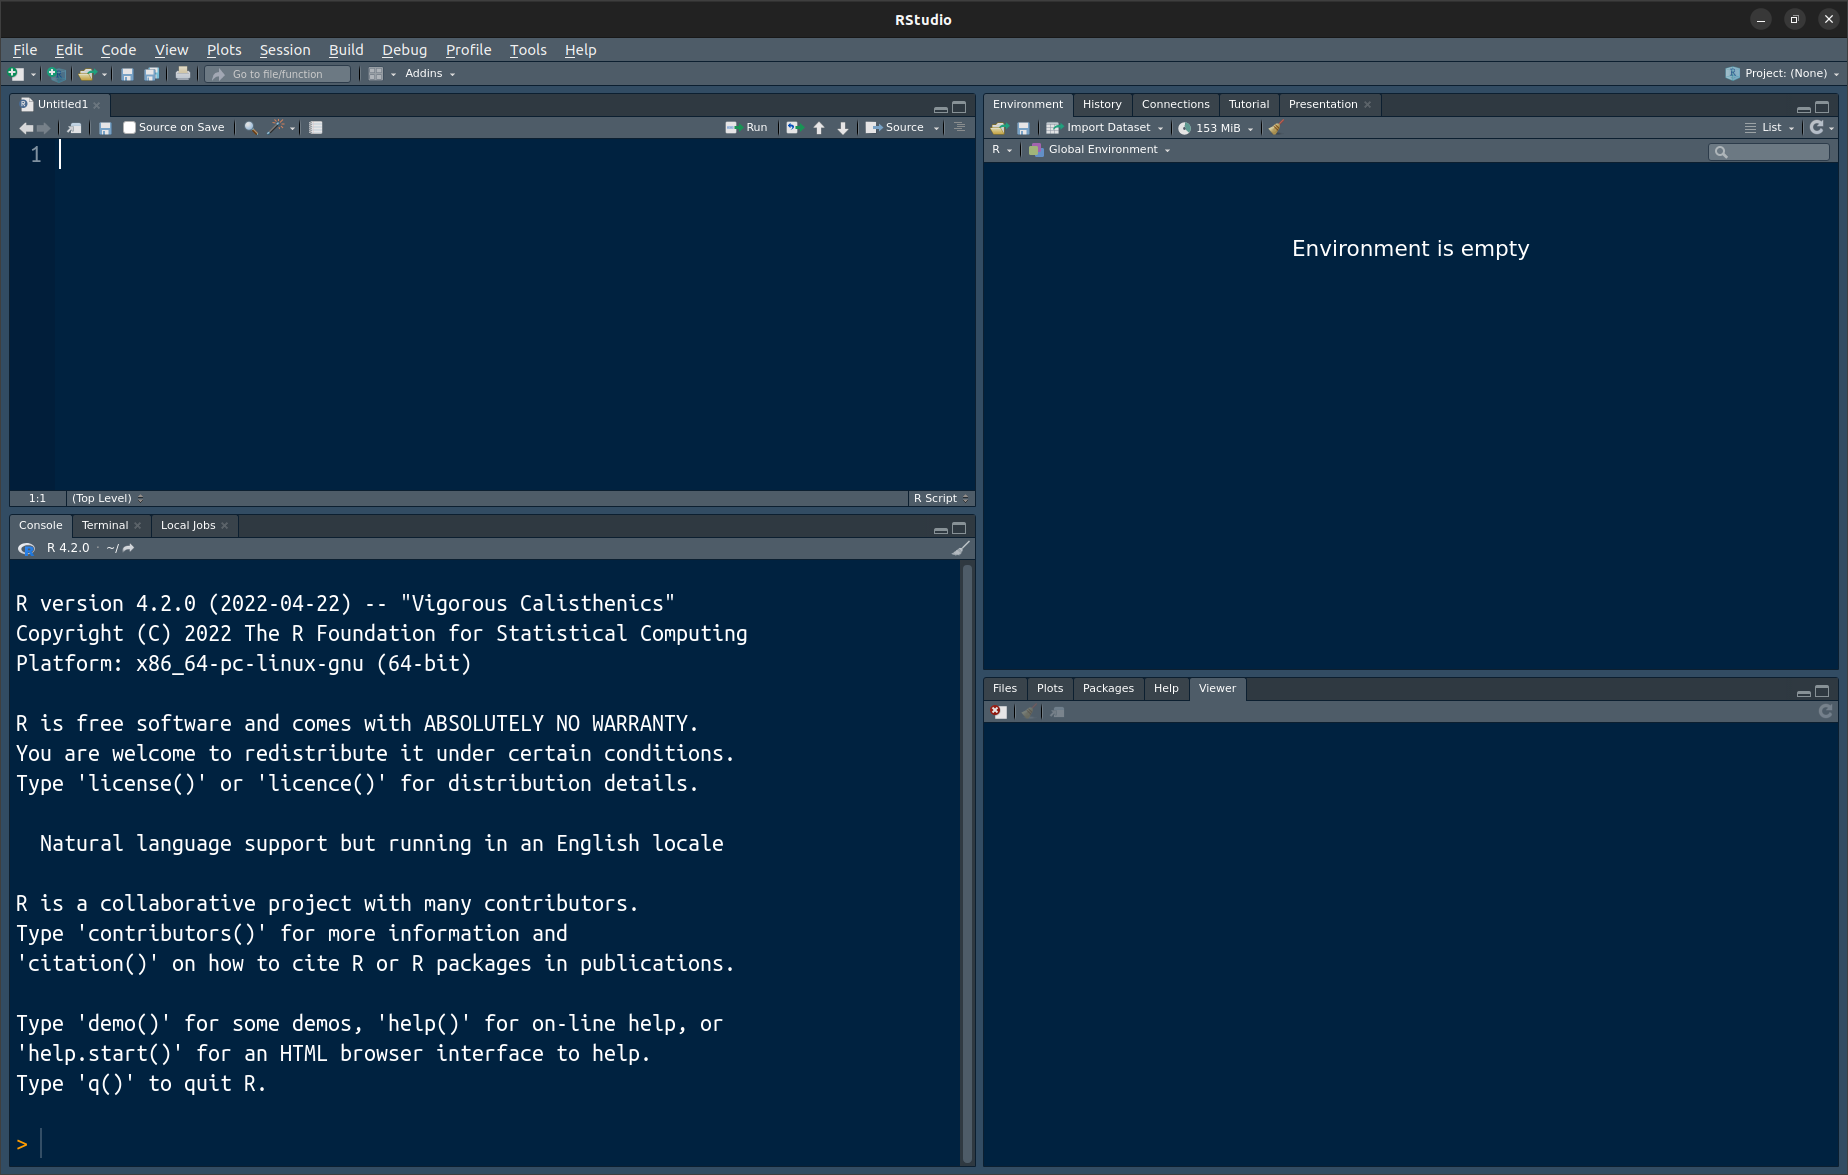
\includegraphics[width = \textwidth]{figs/RStudio.png}
 \caption{RStudio, 
          with the R console in the bottom left, 
          the text editor in the top left, 
          the inventory of the working environment in the top right (currently empty),
          and any plots or opened help pages in the bottom right.}
 \label{fig:rstudio}
\end{figure}

\mypar[Configuring RStudio]{Activity}
In RStudio, and go to \texttt{Tools > Global options...}. 
In the tab \texttt{General, Basic}, make sure to untick the option 
`Restore .RData into workspace at startup' 
and select the option `never' for `Save workspace to .RData on exit'. 
These settings help ensure that you’re starting from a clean slate each time you open RStudio and prevent the results of calculations in previous sessions from messing up your analyses. 
Additionally, in the tab \texttt{Code, Editing}, tick the box next to `Use native pipe operator, |>'. 
We’ll encounter this pipe operator shortly. 
Finally, I recommend setting the default text encoding to UTF-8 under \texttt{Code, Saving}.
\parend

\section{Using R as a calculator}\label{sec:calculator}
\subsection{Arithmetic} \label{sec:arithmetic}
R can be used as a calculator.
To compute sums, products, and quotients, you can enter commands like those
you find below onto the console.
The results aren't part of the commands;
they are displayed once you've entered the command and confirmed it by pressing \textsc{enter}.
R ignores everything to the right of a hash (\#), 
which allows us to add comments to the commands:
\begin{knitrout}
\definecolor{shadecolor}{rgb}{0.969, 0.969, 0.969}\color{fgcolor}\begin{kframe}
\begin{alltt}
\hlnum{10} \hlopt{+} \hlnum{7}     \hlcom{# addition}
\end{alltt}
\begin{verbatim}
[1] 17
\end{verbatim}
\begin{alltt}
\hlnum{12} \hlopt{-} \hlnum{28}    \hlcom{# subtraction}
\end{alltt}
\begin{verbatim}
[1] -16
\end{verbatim}
\begin{alltt}
\hlnum{7} \hlopt{*} \hlnum{3.5}    \hlcom{# multiplication}
\end{alltt}
\begin{verbatim}
[1] 24.5
\end{verbatim}
\begin{alltt}
\hlnum{11} \hlopt{/} \hlnum{3}     \hlcom{# usual division}
\end{alltt}
\begin{verbatim}
[1] 3.666667
\end{verbatim}
\begin{alltt}
\hlnum{6}\hlopt{^}\hlnum{3}        \hlcom{# exponentiation}
\end{alltt}
\begin{verbatim}
[1] 216
\end{verbatim}
\begin{alltt}
\hlnum{10}\hlopt{^}\hldef{(}\hlopt{-}\hlnum{2}\hldef{)}    \hlcom{# = 1/10^2 = 1/100}
\end{alltt}
\begin{verbatim}
[1] 0.01
\end{verbatim}
\begin{alltt}
\hlnum{4}\hlopt{^}\hlnum{0}        \hlcom{# x^0 = 1; R uses the convention 0^0 = 1.}
\end{alltt}
\begin{verbatim}
[1] 1
\end{verbatim}
\begin{alltt}
\hlkwd{sqrt}\hldef{(}\hlnum{16}\hldef{)}   \hlcom{# square root}
\end{alltt}
\begin{verbatim}
[1] 4
\end{verbatim}
\begin{alltt}
\hlkwd{log}\hldef{(}\hlnum{16}\hldef{,} \hlnum{2}\hldef{)} \hlcom{# logarithm base 2 of 16, i.e., 2^4 = 16}
\end{alltt}
\begin{verbatim}
[1] 4
\end{verbatim}
\begin{alltt}
\hlkwd{log}\hldef{(}\hlnum{16}\hldef{)}    \hlcom{# natural logarithm of 16 (i.e., using base e =~ 2.72)}
\end{alltt}
\begin{verbatim}
[1] 2.772589
\end{verbatim}
\begin{alltt}
\hlkwd{log2}\hldef{(}\hlnum{16}\hldef{)}   \hlcom{# shorthand for logarithm base 2}
\end{alltt}
\begin{verbatim}
[1] 4
\end{verbatim}
\begin{alltt}
\hlkwd{log10}\hldef{(}\hlnum{16}\hldef{)}  \hlcom{# shorthand for logarithm base 10}
\end{alltt}
\begin{verbatim}
[1] 1.20412
\end{verbatim}
\begin{alltt}
\hlkwd{ceiling}\hldef{(}\hlnum{2.3}\hldef{)} \hlcom{# rounding up}
\end{alltt}
\begin{verbatim}
[1] 3
\end{verbatim}
\begin{alltt}
\hlkwd{floor}\hldef{(}\hlnum{11.7}\hldef{)}  \hlcom{# rounding down}
\end{alltt}
\begin{verbatim}
[1] 11
\end{verbatim}
\begin{alltt}
\hlkwd{round}\hldef{(}\hlnum{2.3}\hldef{)}   \hlcom{# symmetric rounding}
\end{alltt}
\begin{verbatim}
[1] 2
\end{verbatim}
\begin{alltt}
\hlkwd{round}\hldef{(}\hlnum{2.7}\hldef{)}
\end{alltt}
\begin{verbatim}
[1] 3
\end{verbatim}
\begin{alltt}
\hlkwd{round}\hldef{(}\hlnum{2.5}\hldef{)}   \hlcom{# if ~.5: round to the nearest even integer}
\end{alltt}
\begin{verbatim}
[1] 2
\end{verbatim}
\begin{alltt}
\hlkwd{round}\hldef{(}\hlnum{3.5}\hldef{)}
\end{alltt}
\begin{verbatim}
[1] 4
\end{verbatim}
\begin{alltt}
\hlkwd{abs}\hldef{(}\hlopt{-}\hlnum{3}\hldef{)}  \hlcom{# absolute value}
\end{alltt}
\begin{verbatim}
[1] 3
\end{verbatim}
\begin{alltt}
\hlkwd{sign}\hldef{(}\hlopt{-}\hlnum{3}\hldef{)} \hlcom{# sign}
\end{alltt}
\begin{verbatim}
[1] -1
\end{verbatim}
\begin{alltt}
\hlkwd{sign}\hldef{(}\hlnum{3}\hldef{)}
\end{alltt}
\begin{verbatim}
[1] 1
\end{verbatim}
\begin{alltt}
\hlkwd{sign}\hldef{(}\hlnum{0}\hldef{)}
\end{alltt}
\begin{verbatim}
[1] 0
\end{verbatim}
\end{kframe}
\end{knitrout}

R respects the usual order of operations (e.g., multiplication before addition).
To override this order, you can use round brackets or braces:
\begin{knitrout}
\definecolor{shadecolor}{rgb}{0.969, 0.969, 0.969}\color{fgcolor}\begin{kframe}
\begin{alltt}
\hlnum{4} \hlopt{+} \hlnum{8} \hlopt{*} \hlnum{2}
\end{alltt}
\begin{verbatim}
[1] 20
\end{verbatim}
\begin{alltt}
\hldef{(}\hlnum{4} \hlopt{+} \hlnum{8}\hldef{)} \hlopt{*} \hlnum{2}
\end{alltt}
\begin{verbatim}
[1] 24
\end{verbatim}
\begin{alltt}
\hldef{\{}\hlnum{4} \hlopt{+} \hlnum{8}\hldef{\}} \hlopt{*} \hlnum{2}
\end{alltt}
\begin{verbatim}
[1] 24
\end{verbatim}
\end{kframe}
\end{knitrout}

\mypar[Roots]{*Remark}
The result of $\sqrt{-3}$ is \texttt{NaN} (\textit{not a number})
as there is no real number $x$ such that $x^2 = -3$:
\begin{knitrout}
\definecolor{shadecolor}{rgb}{0.969, 0.969, 0.969}\color{fgcolor}\begin{kframe}
\begin{alltt}
\hlkwd{sqrt}\hldef{(}\hlopt{-}\hlnum{3}\hldef{)}
\end{alltt}
\begin{verbatim}
[1] NaN
\end{verbatim}
\end{kframe}
\end{knitrout}
In the complex numbers, however, such a number does exist.
(More precisely, there exist two such numbers, namely $0 \pm \sqrt{3}\textrm{i}$.)
We won't need complex numbers in this course, so we won't explore them further.

To take arbitrary roots of non-negative number,
note that $\sqrt[n]{x} = x^{1/n}$.
Hence, we may compute $\sqrt[3]{216}$ as $216^{1/3}$:
\begin{knitrout}
\definecolor{shadecolor}{rgb}{0.969, 0.969, 0.969}\color{fgcolor}\begin{kframe}
\begin{alltt}
\hlnum{216} \hlopt{^} \hldef{(}\hlnum{1}\hlopt{/}\hlnum{3}\hldef{)}
\end{alltt}
\begin{verbatim}
[1] 6
\end{verbatim}
\end{kframe}
\end{knitrout}
To take arbitrary roots of negative numbers (e.g., $\sqrt[3]{-8}$),
we'd have to take a detour via the complex numbers, even though real solutions
may exist ($(-2)^3 = -8$).
\parend

\mypar[Scientific notation]{Remark}
If we compute $3328^{27}$, 
the result is displayed as \texttt{1.26e+95}.\footnote{The numbers in the running text don't always correspond exactly to the numbers in the R output since I tend to round them more aggressively.}
\begin{knitrout}
\definecolor{shadecolor}{rgb}{0.969, 0.969, 0.969}\color{fgcolor}\begin{kframe}
\begin{alltt}
\hlnum{3328}\hlopt{^}\hlnum{27}
\end{alltt}
\begin{verbatim}
[1] 1.255884e+95
\end{verbatim}
\end{kframe}
\end{knitrout}
This notation is known as \term{scientific notation}
and is to be read as $1.26 \cdot 10^{95}$---that is, as $1.26$ but with the decimal
point moved 95 places to the right.
The result of $2^{-21}$ is displayed as \texttt{4.8e-07},
which is to be read as $4.8 \cdot 10^{-7}$---that is, as $4.8$ but with the decimal
point moved seven places to the left ($0.00000048$).
\begin{knitrout}
\definecolor{shadecolor}{rgb}{0.969, 0.969, 0.969}\color{fgcolor}\begin{kframe}
\begin{alltt}
\hlnum{2}\hlopt{^}\hldef{(}\hlopt{-}\hlnum{21}\hldef{)}
\end{alltt}
\begin{verbatim}
[1] 4.768372e-07
\end{verbatim}
\end{kframe}
\end{knitrout}
\parend

\mypar[Help pages]{Remark}
In principle, every R function has a help page.
You can display this help page by typing \texttt{?function\_name} at the console.
It takes some practice to efficiently read a help page,
so let's take a closer look at the rounding function \texttt{round()}:
\begin{knitrout}
\definecolor{shadecolor}{rgb}{0.969, 0.969, 0.969}\color{fgcolor}\begin{kframe}
\begin{alltt}
\hlopt{?}\hldef{round} \hlcom{# help page not shown in script}
\end{alltt}
\end{kframe}
\end{knitrout}
This help page consists of nine sections.
Five of these can be found on most help pages:
\begin{enumerate}
  \item Description: A crisp description of the function.

  \item Usage: Which parameters does the function have?
  The function \texttt{round()} has two parameters:
  \texttt{x} and \texttt{digits}.
  If no value is specified for \texttt{digits}, 
  the value 0 is used by default.

  \item Arguments: Brief specifications of the expected parameter values.

  \item Details: More details about the function.
  For instance, the Details section on the help page for \texttt{round()}
  explains how and why $-1.5$ is rounded
  and why the command \texttt{round(0.15, 1)} can produce unexpected results.

  \item Examples: Click on `Run examples' to see the output generated
  by these examples.
\end{enumerate}

The help page for the addition operator \texttt{+} can be displayed
by typing \texttt{?"+"} at the console.\parend

% \subsection{Graphs of functions}
% With the command below, you can draw the graph of a mathematical function;
% see Figure \ref{fig:curve}.
% Type this command in RStudio's text editor (top left panel).
% And I mean `type', not `copy-paste'!
% You'll learn more by typing than by copy-pasting.
% Then move the text cursor to one of the lines that make up the command
% and hit \textsc{ctrl + enter} (on Windows and Linux)
% or \textsc{cmd + enter} (on macOS).
% This relays the command to the console (bottom left).
% While you could enter this command directly onto the console,
% you should make a habit of working in the text editor.
% This makes it easier to find and rectify errors.
% Moreover, working in the editor makes it easy to document your analyses
% as you can save your scripts.
% 
% <<Curve, fig.cap = "Graph of the function $x \\mapsto 2^{-\\frac{x^2}{2}}\\frac{x}{1 + x^2}$.\\label{fig:curve}", fig.asp=0.7>>=
% curve(2^(-x^2/2) * x/(1 + x^2),
%       from = -5, to = 5,
%       xlab = "x", ylab = "f(x)")
% @
% 
% Graphs drawn using \texttt{curve()} can give the impression that the function
% being drawn is defined everywhere, even if this isn't the case.
% For instance, the function $x \mapsto \frac{\sin(x)}{x}$ isn't defined at $x = 0$,
% since you can't divide by 0.
% If you draw the graph of this function, however, you might conclude that $0 \mapsto 1$.
% Here, it's a good idea to draw an empty circle at the coordinates $(0, 1)$ to
% highlight that the function isn't defined at $x = 0$:
% <<eval = FALSE>>=
% curve(sin(x)/x,
%       from = -12, to = 12,
%       xlab = "x", ylab = "f(x)")
% # Use 'cex' (character expansion) to specify the size
% points(0, 1, cex = 2)
% @
% 
% Additionally, graphs of functions drawn using \texttt{curve()}
% can look continuous (i.e., without gaps).
% But i
% Weiter sieht jeder mit \texttt{curve()} gezeichnete Funktionsgraph
% stetig, also lückenlos, aus.
% Aber beispielsweise die Vorzeichen- (oder Signum-)Funktion,
% \[
%   \textrm{sgn}(x) := \begin{cases} -1,  & \textrm{falls $x < 0$,} \\
%                                   0,    & \textrm{falls $x = 0$,} \\
%                                   1,    & \textrm{falls $x > 0$,}
%                     \end{cases}
% \]
% hat eine Unstetigkeitsstelle, also einen Sprung, bei $x = 0$.
% Wenn Sie den Graphen
% dieser Funktion zeichnen würden, so würde es aussehen, als wäre dieser zwar
% stark wachsend um den Nullpunkt herum,
% aber schon ununterbrochen.
% Um den richtigen Graphen dieser Funktion zu zeichnen,
% reicht den \texttt{curve()}-Befehl nicht aus.
% Stattdessen müssen wir uns den Graphen mit etwas mehr Mühe zusammenbasteln:
% <<eval = FALSE>>=
% # leere Leinwand zeichnen
% plot(0, 0,
%      type = "n", # nur Leinwand zeichnen
%      xlim = c(-3, 3),
%      ylim = c(-1.2, 1.2),
%      xlab = "x", ylab = "f(x)")
% # Funktionswerte für negative Zahlen
% segments(x0 = -4, x1 = 0, y0 = -1) # siehe ?segments
% # für positive Zahlen
% segments(x0 = 0, x1 = 4, y0 = 1)
% # für 0
% points(0, 0, pch = 16) # siehe ?points
% points(0, -1, pch = 1)
% points(0, 1, pch = 1)
% @

% 
% \mypar[grafische Parameter einstellen]{Bemerkung}
%   Wenn Sie den Graphen in Abbildung \ref{fig:curve} selber zeichnen,
%   so werden Sie feststellen, dass das Resultat bei Ihnen etwas anders aussieht.
%   Unter anderem werden die Werte auf der $y$-Achse bei Ihnen vertikal statt
%   horizontal orientiert sein.
%   Wie mit \texttt{curve()} oder \texttt{plot()} gezeichnete Graphen aussehen sollten,
%   können Sie mit \texttt{par()} einstellen.
%   Wenn Sie meine Einstellungen übernehmen möchten, können Sie zunächst
%   den folgenden Befehl ausführen und dann den Graphen nochmals zeichnen.
%   
% <<eval = FALSE>>=
% par(las = 1,
%     bty = "l",
%     mar = c(3, 3.5, 2, 1),
%     mgp = c(2, 0.3, 0),
%     tck = -0.01,
%     cex = 0.8)
% @
% 
% Siehe \texttt{?par} für weitere Infos.
% \parend
% 
\subsection{Vectorised operations}
In R, a \term{vector} is a specific number of numbers (or other objects)
that are grouped together.
Numbers and other objects can be grouped together into vector using the function \texttt{c()}
(\textit{combine}).
The object so created can be given a name by means of the assignment operator \texttt{<-};
here, we'll call it \texttt{a}:
\begin{knitrout}
\definecolor{shadecolor}{rgb}{0.969, 0.969, 0.969}\color{fgcolor}\begin{kframe}
\begin{alltt}
\hldef{a} \hlkwb{<-} \hlkwd{c}\hldef{(}\hlopt{-}\hlnum{4}\hldef{,} \hlnum{2}\hldef{,} \hlnum{0.3}\hldef{,} \hlnum{2014}\hldef{)}
\end{alltt}
\end{kframe}
\end{knitrout}
The vector known as \texttt{a} now contains the four numbers listed.
We can display the vector in its entirety by typing its name at the prompt:
\begin{knitrout}
\definecolor{shadecolor}{rgb}{0.969, 0.969, 0.969}\color{fgcolor}\begin{kframe}
\begin{alltt}
\hldef{a}
\end{alltt}
\begin{verbatim}
[1]   -4.0    2.0    0.3 2014.0
\end{verbatim}
\end{kframe}
\end{knitrout}
Using \texttt{a[i]}, we can select the vector's $i$-th entry (i.e., $a_i$),
$1 \leq i \leq n$. 
Note that R uses \term{one-based indexing}, meaning that a vector's first component
is accessed using $i = 1$. 
This contrasts with the many other computer languages that use \term{zero-based indexing},
that is, they access a vector's first component using $i = 0$.
\begin{knitrout}
\definecolor{shadecolor}{rgb}{0.969, 0.969, 0.969}\color{fgcolor}\begin{kframe}
\begin{alltt}
\hldef{a[}\hlnum{1}\hldef{]}         \hlcom{# 1st component}
\end{alltt}
\begin{verbatim}
[1] -4
\end{verbatim}
\begin{alltt}
\hldef{a[}\hlopt{-}\hlnum{3}\hldef{]}        \hlcom{# all components except for the 3rd one}
\end{alltt}
\begin{verbatim}
[1]   -4    2 2014
\end{verbatim}
\begin{alltt}
\hldef{a[}\hlkwd{c}\hldef{(}\hlnum{2}\hldef{,} \hlnum{4}\hldef{)]}   \hlcom{# using c() to extract several components}
\end{alltt}
\begin{verbatim}
[1]    2 2014
\end{verbatim}
\begin{alltt}
\hldef{a[}\hlopt{-}\hlkwd{c}\hldef{(}\hlnum{2}\hldef{,} \hlnum{4}\hldef{)]}  \hlcom{# all components except for the 2nd and 4th one}
\end{alltt}
\begin{verbatim}
[1] -4.0  0.3
\end{verbatim}
\end{kframe}
\end{knitrout}

The sum of all components of a vector $a$ is expressed in \term{capital sigma notation} as
\[
  \sum_{i=1}^n a_i := a_1 + a_2 + \dots + a_n,
\]
where $n$ is the number of components of $a$.
It can easily be computed using \texttt{sum()}:
\begin{knitrout}
\definecolor{shadecolor}{rgb}{0.969, 0.969, 0.969}\color{fgcolor}\begin{kframe}
\begin{alltt}
\hlkwd{sum}\hldef{(a)}
\end{alltt}
\begin{verbatim}
[1] 2012.3
\end{verbatim}
\end{kframe}
\end{knitrout}
The product of all components, i.e.,
\[
  \prod_{i=1}^n a_i := a_1 \cdot a_2 \cdot \dots \cdot a_n,
\]
can be computed using \texttt{prod()}:
\begin{knitrout}
\definecolor{shadecolor}{rgb}{0.969, 0.969, 0.969}\color{fgcolor}\begin{kframe}
\begin{alltt}
\hlkwd{prod}\hldef{(a)}
\end{alltt}
\begin{verbatim}
[1] -4833.6
\end{verbatim}
\end{kframe}
\end{knitrout}

The length of a vector, that is, the number of components it has,
can be obtained using \texttt{length()};
its maximum and minimum using \texttt{max()} and \texttt{min()}, respectively:
\begin{knitrout}
\definecolor{shadecolor}{rgb}{0.969, 0.969, 0.969}\color{fgcolor}\begin{kframe}
\begin{alltt}
\hlkwd{length}\hldef{(a)}
\end{alltt}
\begin{verbatim}
[1] 4
\end{verbatim}
\begin{alltt}
\hlkwd{max}\hldef{(a)}
\end{alltt}
\begin{verbatim}
[1] 2014
\end{verbatim}
\begin{alltt}
\hlkwd{min}\hldef{(a)}
\end{alltt}
\begin{verbatim}
[1] -4
\end{verbatim}
\end{kframe}
\end{knitrout}

The operations from Section \ref{sec:arithmetic} can also be applied to vectors.
In this case, they are applied componentwise:
\begin{knitrout}
\definecolor{shadecolor}{rgb}{0.969, 0.969, 0.969}\color{fgcolor}\begin{kframe}
\begin{alltt}
\hlnum{2} \hlopt{*} \hldef{a}
\end{alltt}
\begin{verbatim}
[1]   -8.0    4.0    0.6 4028.0
\end{verbatim}
\begin{alltt}
\hldef{a} \hlopt{-} \hlnum{7}
\end{alltt}
\begin{verbatim}
[1]  -11.0   -5.0   -6.7 2007.0
\end{verbatim}
\begin{alltt}
\hlkwd{sqrt}\hldef{(a)} \hlcom{# warning due to square root of negative number}
\end{alltt}
\begin{verbatim}
[1]        NaN  1.4142136  0.5477226 44.8776113
\end{verbatim}
\begin{alltt}
\hlkwd{log}\hldef{(a,} \hlnum{2}\hldef{)} \hlcom{# warning due to logarithm of non-positive number}
\end{alltt}
\begin{verbatim}
[1]       NaN  1.000000 -1.736966 10.975848
\end{verbatim}
\end{kframe}
\end{knitrout}

If we define a second vector of the same length,
we can run certain operations on the corresponding components:
\begin{knitrout}
\definecolor{shadecolor}{rgb}{0.969, 0.969, 0.969}\color{fgcolor}\begin{kframe}
\begin{alltt}
\hldef{b} \hlkwb{<-} \hlkwd{c}\hldef{(}\hlnum{3}\hldef{,} \hlnum{8.2}\hldef{,} \hlopt{-}\hlnum{1.2}\hldef{,} \hlkwd{sqrt}\hldef{(}\hlnum{20}\hldef{))}
\hldef{a} \hlopt{-} \hldef{b}
\end{alltt}
\begin{verbatim}
[1]   -7.000   -6.200    1.500 2009.528
\end{verbatim}
\begin{alltt}
\hldef{a} \hlopt{+} \hldef{b}
\end{alltt}
\begin{verbatim}
[1]   -1.000   10.200   -0.900 2018.472
\end{verbatim}
\begin{alltt}
\hldef{a} \hlopt{/} \hldef{b}
\end{alltt}
\begin{verbatim}
[1]  -1.3333333   0.2439024  -0.2500000 450.3440907
\end{verbatim}
\begin{alltt}
\hldef{a} \hlopt{*} \hldef{b}
\end{alltt}
\begin{verbatim}
[1]  -12.000   16.400   -0.360 9006.882
\end{verbatim}
\begin{alltt}
\hldef{a}\hlopt{^}\hldef{b}
\end{alltt}
\begin{verbatim}
[1] -6.400000e+01  2.940668e+02  4.240865e+00  5.973146e+14
\end{verbatim}
\end{kframe}
\end{knitrout}

To compute the componentwise maximum or minimum of two or more vectors,
we need to use \texttt{pmax()} or \texttt{pmin()}, respectively (\textit{p} for \textit{parallel}):
\begin{knitrout}
\definecolor{shadecolor}{rgb}{0.969, 0.969, 0.969}\color{fgcolor}\begin{kframe}
\begin{alltt}
\hlkwd{pmax}\hldef{(a, b)}
\end{alltt}
\begin{verbatim}
[1]    3.0    8.2    0.3 2014.0
\end{verbatim}
\begin{alltt}
\hlkwd{pmin}\hldef{(a, b)}
\end{alltt}
\begin{verbatim}
[1] -4.000000  2.000000 -1.200000  4.472136
\end{verbatim}
\end{kframe}
\end{knitrout}
The function \texttt{max()} and \texttt{min()} compute the overall maximum and minimum
entry across all vectors:
\begin{knitrout}
\definecolor{shadecolor}{rgb}{0.969, 0.969, 0.969}\color{fgcolor}\begin{kframe}
\begin{alltt}
\hlkwd{max}\hldef{(a, b)}
\end{alltt}
\begin{verbatim}
[1] 2014
\end{verbatim}
\end{kframe}
\end{knitrout}

\mypar[Vectors of different lengths]{Remark}
  The second vector doesn't have to have the same length as the first
  when running vectorised operations.
  But when the vectors involved have different lengths, it can be difficult to
  anticipate the results.
  By way of an example, we define a vector $d$ that has three components
  and add this vector to the vector $a$, which has four components.
  (We don't name the vector \texttt{c} as there exists an R function called \texttt{c()}.)
\begin{knitrout}
\definecolor{shadecolor}{rgb}{0.969, 0.969, 0.969}\color{fgcolor}\begin{kframe}
\begin{alltt}
\hldef{d} \hlkwb{<-} \hlkwd{c}\hldef{(}\hlnum{3}\hldef{,} \hlnum{8.2}\hldef{,} \hlopt{-}\hlnum{1.2}\hldef{)}
\hldef{a} \hlopt{+} \hldef{d}
\end{alltt}
\begin{verbatim}
[1]   -1.0   10.2   -0.9 2017.0
\end{verbatim}
\end{kframe}
\end{knitrout}
  Since the vectors involved have different lengths, and one of the lengths
  isn't a multiple of the other,
  the fourth addition uses
  the fourth element of the first vector and the first element of the second vector.
  This is bound to cause confusion.
  
  At least in this example, a warning pops up.
  However, if one of the vectors' length had been a multiple of the other's,
  then this warning wouldn't have appeared---despite the problem persisting!
  
  Don't put yourself in this situation.
\parend

\mypar[Sequences]{Remark}
  We've seen that we can use \texttt{c()} to define vectors.
  If you want to define a vector that represents a sequence, 
  more practical alternatives are available.
\begin{knitrout}
\definecolor{shadecolor}{rgb}{0.969, 0.969, 0.969}\color{fgcolor}\begin{kframe}
\begin{alltt}
\hldef{z} \hlkwb{<-} \hlnum{3}\hlopt{:}\hlnum{12}
\hldef{z}
\end{alltt}
\begin{verbatim}
 [1]  3  4  5  6  7  8  9 10 11 12
\end{verbatim}
\begin{alltt}
\hldef{z} \hlkwb{<-} \hlnum{7}\hlopt{:-}\hlnum{1}
\hldef{z}
\end{alltt}
\begin{verbatim}
[1]  7  6  5  4  3  2  1  0 -1
\end{verbatim}
\begin{alltt}
\hldef{z} \hlkwb{<-} \hlkwd{seq}\hldef{(}\hlkwc{from} \hldef{=} \hlnum{1}\hldef{,} \hlkwc{to} \hldef{=} \hlnum{3.5}\hldef{,} \hlkwc{by} \hldef{=} \hlnum{0.25}\hldef{)}
\hldef{z}
\end{alltt}
\begin{verbatim}
 [1] 1.00 1.25 1.50 1.75 2.00 2.25 2.50 2.75 3.00 3.25 3.50
\end{verbatim}
\begin{alltt}
\hldef{z} \hlkwb{<-} \hlkwd{seq}\hldef{(}\hlkwc{from} \hldef{=} \hlnum{0}\hldef{,} \hlkwc{to} \hldef{=} \hlnum{2}\hldef{,} \hlkwc{length.out} \hldef{=} \hlnum{7}\hldef{)}
\hldef{z}
\end{alltt}
\begin{verbatim}
[1] 0.0000000 0.3333333 0.6666667 1.0000000 1.3333333
[6] 1.6666667 2.0000000
\end{verbatim}
\begin{alltt}
\hldef{z} \hlkwb{<-} \hlkwd{seq}\hldef{(}\hlkwc{to} \hldef{=} \hlnum{2}\hldef{,} \hlkwc{by} \hldef{=} \hlnum{12}\hldef{,} \hlkwc{length.out} \hldef{=} \hlnum{5}\hldef{)}
\hldef{z}
\end{alltt}
\begin{verbatim}
[1] -46 -34 -22 -10   2
\end{verbatim}
\begin{alltt}
\hldef{z} \hlkwb{<-} \hlkwd{seq_len}\hldef{(}\hlnum{5}\hldef{)}
\hldef{z}
\end{alltt}
\begin{verbatim}
[1] 1 2 3 4 5
\end{verbatim}
\end{kframe}
\end{knitrout}
  Figure out what each of these commands does.
\parend
 
\section{*R as a programming language}\label{sec:rprogramming}
We can extend the functionality of R by writing our own functions.
We'll take a look at a few examples to show how this works;
more examples follow in later chapters.

\mypar[Scalar product]{Example} 
Let $\bm x = (x_1, \dots, x_n)$ and $\bm y = (y_1, \dots, y_n)$ both be vectors
with $n \geq 1$ real numbers as their components.
The so-called (standard) \term{scalar product} assigns
to this pair of vectors a real number (i.e., a scalar, hence the name), namely
\[
  \langle \bm x, \bm y \rangle := \bm x \cdot \bm y := \sum_{i=1}^n x_iy_i = x_1y_1 + x_2y_2 + \dots + x_ny_n.
\]
The standard scalar product is also known as the \term{dot product} due to one of the ways 
it is commonly represented (namely $\bm x \cdot \bm y$).

Let's write a simple R function \texttt{dot()} that takes two vectors as its arguments
and outputs their dot product.
To this end, we use the reserved keyword \texttt{function()} and specify that our
function takes two inputs, \texttt{x} and \texttt{y}.
The function computes the componentwise product of the input vectors,
sums its entries, and outputs this sum:

\begin{knitrout}
\definecolor{shadecolor}{rgb}{0.969, 0.969, 0.969}\color{fgcolor}\begin{kframe}
\begin{alltt}
\hldef{dot} \hlkwb{<-} \hlkwa{function}\hldef{(}\hlkwc{x}\hldef{,} \hlkwc{y}\hldef{) \{}
  \hlkwd{sum}\hldef{(x} \hlopt{*} \hldef{y)}
\hldef{\}}
\end{alltt}
\end{kframe}
\end{knitrout}

We can use the new function \texttt{dot()} as we would any other R function:
\begin{knitrout}
\definecolor{shadecolor}{rgb}{0.969, 0.969, 0.969}\color{fgcolor}\begin{kframe}
\begin{alltt}
\hldef{a} \hlkwb{<-} \hlkwd{c}\hldef{(}\hlnum{4}\hldef{,} \hlnum{2}\hldef{,} \hlopt{-}\hlnum{1}\hldef{)}
\hldef{b} \hlkwb{<-} \hlkwd{c}\hldef{(}\hlnum{8}\hldef{,} \hlopt{-}\hlnum{2}\hldef{,} \hlnum{2}\hldef{)}
\hlkwd{dot}\hldef{(a, b)}
\end{alltt}
\begin{verbatim}
[1] 26
\end{verbatim}
\end{kframe}
\end{knitrout}

We can add some further features to this basic function.
For instance, \texttt{dot()} should only work on numerical vectors
(as opposed to on vectors of characters, or on other objects altogether)
of the same length.
Using \textit{if}-clauses and the \texttt{stop()} keyword,
we can check if the input to the \texttt{dot()} function fulfils 
these criteria.

\begin{knitrout}
\definecolor{shadecolor}{rgb}{0.969, 0.969, 0.969}\color{fgcolor}\begin{kframe}
\begin{alltt}
\hldef{dot} \hlkwb{<-} \hlkwa{function}\hldef{(}\hlkwc{x}\hldef{,} \hlkwc{y}\hldef{) \{}
  \hlkwa{if} \hldef{(}\hlopt{!}\hlkwd{is.numeric}\hldef{(x))} \hlkwd{stop}\hldef{(}\hlsng{"First input isn't numeric."}\hldef{)}
  \hlkwa{if} \hldef{(}\hlopt{!}\hlkwd{is.numeric}\hldef{(y))} \hlkwd{stop}\hldef{(}\hlsng{"Second input isn't numeric."}\hldef{)}
  \hlkwa{if} \hldef{(}\hlkwd{length}\hldef{(x)} \hlopt{!=} \hlkwd{length}\hldef{(y))} \hlkwd{stop}\hldef{(}\hlsng{"Inputs have different lengths."}\hldef{)}
  \hlkwd{sum}\hldef{(x} \hlopt{*} \hldef{y)}
\hldef{\}}
\end{alltt}
\end{kframe}
\end{knitrout}

If the input vectors are incompatible, \texttt{dot()} now generates
an error:
\begin{knitrout}
\definecolor{shadecolor}{rgb}{0.969, 0.969, 0.969}\color{fgcolor}\begin{kframe}
\begin{alltt}
\hldef{a} \hlkwb{<-} \hlkwd{c}\hldef{(}\hlnum{4}\hldef{,} \hlnum{2}\hldef{,} \hlopt{-}\hlnum{1}\hldef{)}
\hldef{b} \hlkwb{<-} \hlkwd{c}\hldef{(}\hlnum{8}\hldef{,} \hlopt{-}\hlnum{2}\hldef{)}
\hlkwd{dot}\hldef{(a, b)}
\end{alltt}


{\ttfamily\noindent\bfseries\color{errorcolor}{Error in dot(a, b): Inputs have different lengths.}}\end{kframe}
\end{knitrout}
\parend

\mypar[Euclidean norm]{Exercise}
  Let $\bm x = (x_1, \dots, x_n)$ be a numerical vector 
  with $n \geq 1$ real numbers as its components.
  The vector's \term{Euclidean norm} is defined as
  \[
    \norm{\bm x} := \sqrt{\langle \bm x, \bm x \rangle},
  \]
  where $\langle \cdot, \cdot \rangle$ is the standard
  scalar product from the previous example.
  A vector's Euclidean norm tells you how far the 
  vector is removed from the coordinate system's origin.
  
  Write a function \texttt{norm()} that takes one numerical
  input vector and outputs its norm.
  Use the \texttt{dot()} function from the previous example when defining
  your function.
  
  Hint: The norm of the vector \texttt{a} from the previous example is about 4.583.
\parend

\mypar[Decumulation]{Example}
  Given a numerical vector $\bm x = (x_1, \dots, x_n)$,
  we can compute the vector containing its cumulative sums, i.e.,
  \[
    (x_1, x_1 + x_2, x_1 + x_2 + x_3, \dots, x_1 + \dots + x_n).
  \]
  The built-in function \texttt{cumsum()} does just this:
\begin{knitrout}
\definecolor{shadecolor}{rgb}{0.969, 0.969, 0.969}\color{fgcolor}\begin{kframe}
\begin{alltt}
\hldef{a} \hlkwb{<-} \hlkwd{c}\hldef{(}\hlnum{17}\hldef{,} \hlnum{21}\hldef{,} \hlopt{-}\hlnum{24}\hldef{,} \hlnum{8}\hldef{)}
\hlkwd{cumsum}\hldef{(a)}
\end{alltt}
\begin{verbatim}
[1] 17 38 14 22
\end{verbatim}
\end{kframe}
\end{knitrout}
  What if we want to reverse this operation, i.e., given a vector
  of cumulative sums $\bm x$, 
  we want to reconstruct the original vector, which we'll call $\bm y$?
  Observe that $y_1 = x_1$ and $y_{i} = x_{i} - x_{i-1}$ for $i = 2, \dots, n$.
  Using a \term{\textit{for}-loop}, we can define a function \texttt{decum()}
  that reconstructs the decumulated vector like so:
\begin{knitrout}
\definecolor{shadecolor}{rgb}{0.969, 0.969, 0.969}\color{fgcolor}\begin{kframe}
\begin{alltt}
\hldef{decum} \hlkwb{<-} \hlkwa{function}\hldef{(}\hlkwc{x}\hldef{) \{}
  \hldef{y} \hlkwb{<-} \hlkwd{vector}\hldef{(}\hlkwc{length} \hldef{=} \hlkwd{length}\hldef{(x))}
  \hldef{y[}\hlnum{1}\hldef{]} \hlkwb{<-} \hldef{x[}\hlnum{1}\hldef{]}
  \hlkwa{for} \hldef{(i} \hlkwa{in} \hlnum{2}\hlopt{:}\hlkwd{length}\hldef{(x)) \{}
    \hldef{y[i]} \hlkwb{<-} \hldef{x[i]} \hlopt{-} \hldef{x[i} \hlopt{-} \hlnum{1}\hldef{]}
  \hldef{\}}
  \hldef{y}
\hldef{\}}
\end{alltt}
\end{kframe}
\end{knitrout}

  A quick check shows that this function does the trick:
\begin{knitrout}
\definecolor{shadecolor}{rgb}{0.969, 0.969, 0.969}\color{fgcolor}\begin{kframe}
\begin{alltt}
\hlkwd{decum}\hldef{(}\hlkwd{cumsum}\hldef{(a))} \hlcom{# same as 'a'}
\end{alltt}
\begin{verbatim}
[1]  17  21 -24   8
\end{verbatim}
\end{kframe}
\end{knitrout}
\parend

\section{Add-on packages}
There are thousands of free add-on packages that extend the functionality of R.
We'll use a couple of these throughout this course.

\mypar[Installing the \texttt{tidyverse}]{Activity}
  Use the command below to install the \texttt{tidyverse} suite.
  This is a bundle of different add-on packages that are based on a shared
  philosophy and make working with datasets easier.
\begin{knitrout}
\definecolor{shadecolor}{rgb}{0.969, 0.969, 0.969}\color{fgcolor}\begin{kframe}
\begin{alltt}
\hlkwd{install.package}\hldef{(}\hlsng{"tidyverse"}\hldef{)}
\end{alltt}
\end{kframe}
\end{knitrout}
  You can find manuals, tutorials etc.\ of the packages included in the \texttt{tidyverse}
  at \url{https://www.tidyverse.org/}.
\parend

\mypar[Installing \texttt{here}]{Activity}
  A further useful package we'll use throughout is the \texttt{here} package.
  Install it.
\parend

\mypar[Updating packages]{Remark}
Both R and its add-on packages are in continuous development.
To update the R packages you've installed, you can run
the command \texttt{update.package()}.
To upgrade to a newer version of R itself, I find it easiest
to just uninstall the old version and install the new one from scratch.
In this case, however, you will need to reinstall any add-on packages
you need.
This can be quite cumbersome, which is why I only do it during semester
breaks.

A word of warning, though.
It occurs quite often that your R code won't work as before
when you've updated your packages.
For larger research projects, I recommend ticking the
\texttt{Use renv with this project} option.
Any packages you use in your project will then be stored
along with your project.
Even if you work with newer versions of these packages
in other projects, the old versions will still be used for this one.
This reduces the risk that your R code doesn't work a few years down the line.
For more information, see \url{https://rstudio.github.io/renv/articles/renv.html}.

You can find an overview of the software versions used for this booklet
in the appendix.
Such an overview can be generated using
\begin{knitrout}
\definecolor{shadecolor}{rgb}{0.969, 0.969, 0.969}\color{fgcolor}\begin{kframe}
\begin{alltt}
\hlkwd{sessionInfo}\hldef{()} \hlcom{# output not shown}
\end{alltt}
\end{kframe}
\end{knitrout}
\parend

\mypar[Citing software and packages]{Remark}
  R and R packages are free to use and are mostly developed by other researchers.
  You can acknowledge their help by citing the packages you used.
  You can obtain a reference to R by running the command \texttt{citation()}.
  References to specific packages can be obtained by running the command
  \texttt{citation("packagename")}, e.g.,
\begin{knitrout}
\definecolor{shadecolor}{rgb}{0.969, 0.969, 0.969}\color{fgcolor}\begin{kframe}
\begin{alltt}
\hlkwd{citation}\hldef{(}\hlsng{"tidyverse"}\hldef{)} \hlcom{# output not shown}
\end{alltt}
\end{kframe}
\end{knitrout}
  To obtain a reference to R itself, use
\begin{knitrout}
\definecolor{shadecolor}{rgb}{0.969, 0.969, 0.969}\color{fgcolor}\begin{kframe}
\begin{alltt}
\hlkwd{citation}\hldef{()} \hlcom{# output not shown}
\end{alltt}
\end{kframe}
\end{knitrout}
  
\parend

\section{R projects}
It's convenient to have all scripts, datasets, plots, etc.,
related a project in the same directory.
When working in RStudio, 
I recommend setting up an R project for each project
you're working on.
Projects would include term papers, master theses, course materials,
research projects, etc.
You should also set up an R project for this course.

\mypar[Setting up an R project]{Activity}
  In RStudio, click on
  \texttt{File > New Project..., New Directory, New Project}.
  Navigate to somewhere on your compute where you want to 
  create a new directory and give this directory
  an informative name such as \texttt{statscourse}.
  You will use this directory to store the data, scripts, etc.\
  that you need for this course.
  It's not necessary to tick the option \texttt{Use renv with this project}.
  
  When you’re done, close RStudio. 
  Navigate to the directory you've just created. 
  You should find an \texttt{.Rproj} file there. 
  Double-click it. 
  If all is well, RStudio should fire up.
  Alternatively, you can use \texttt{File > Open Project...} in RStudio.
  
  Once you've opened your project, open the \texttt{Files} tab
  in the bottom right corner.
  Use \texttt{New Folder} to create the subdirectories
  \texttt{data}, \texttt{figs}, \texttt{functions}, and \texttt{assignments}.
  The datasets we'll use should be stored in the subdirectory \texttt{data};
  we'll store the plots we'll create in \texttt{figs};
  \texttt{functions} will contain some custom R functions;
  and you can save your homework assignments in \texttt{assignments}.
\parend

The datasets, custom functions, etc.\ that we'll use are available
from this course's Github page at \url{https://github.com/janhove/AnalysingQuantitativeData/}.

\section{R Markdown reports}
  R scripts can be compiled to reports.
  This is useful for ensuring that your analyses are reproducible:
  Only those commands that are present in the script get compiled,
  and not some commands that you ran but for some reason didn't include 
  in the script.
  Moreover, scripts only compile if all commands can be parsed.
  For this reason, you should submit your homework assignments both
  as an script (with the \texttt{.R} extension) and as a compiled report.
  See the next activity for details.
  
\mypar[Report templates]{Activity}
  Save the \texttt{template.R} file to the \texttt{assignments} subdirectory
  in your R project directory.
  Compile it: \texttt{File > Compile Report\dots}.
  Compare the .R file with the compiled HTML report.
  Use this template for your homework assignments, changing
  dates, names, titles, etc., as necessary.
\parend


\chapter{Working with datasets}\label{ch:datasets}
It's often said that 80\% of data analysis is getting the data in a shape
in which it can be analysed.
The goal of this chapter is to furnish you with the 
basic tools and skills to organise, transform, and query datasets in research contexts. 
We'll work with the \texttt{tidyverse} suite throughout.

\section{Organising datasets}
Let's say we've run a study in which speakers of German read a couple
of words in Swedish and were asked to guess what these words might mean.
An excerpt from the raw data might look like this, with the words having
been shown to the participants in the order in which they are listed:

\begin{itemize}
\item Participant 1034. Woman, 51 years.
\begin{itemize}
\item Word: \textit{söka}. Translation: \textit{Socken} (incorrect).
\item Word: \textit{försiktig}. Translation: \textit{vorsichtig} (correct).
\item Word: \textit{mjölk}. Translation: \textit{Milch} (correct).
\item Word: \textit{behärska}. No translation provided.
\item Word: \textit{fiende}. Translation: \textit{finden} (incorrect).
\end{itemize}

\item Participant 2384. Woman, 27 years.
\begin{itemize}
\item Word: \textit{fiende}. No translation provided.
\item Word: \textit{behärska}. No translation provided.
\item Word: \textit{försiktig}. Translation: \textit{vorsichtig} (correct).
\item Word: \textit{mjölk}. Translation: \textit{Milch} (correct).
\item Word: \textit{söka}. Translation: \textit{Socke} (incorrect).
\end{itemize}

\item Participant 8667. Woman, 27 years.
\begin{itemize}
\item Word: \textit{mjölk}. Translation: \textit{Milch} (correct).
\item Word: \textit{behärska}. No translation provided.
\item Word: \textit{fiende}. Translation: \textit{finden} (incorrect).
\item Word: \textit{söka}. Translation: \textit{suchen} (correct).
\item Word: \textit{försiktig}. Translation: \textit{vorsichtig} (correct).
\end{itemize}

\item Participant 5901. Man, 15 years.
\begin{itemize}
\item Word: \textit{behärska}. Translation: \textit{beherrschen} (correct).
\item Word: \textit{mjölk}. Translation: \textit{milch} (sic.) (correct).
\item Word: \textit{försiktig}. Translation: \textit{vorsichtig} (correct).
\item Word: \textit{fiende}. Translation: \textit{feinde} (sic.) (correct; actually \textit{Feind}).
\item Word: \textit{söka}. Translation: \textit{socken} (sic.) (incorrect).
\end{itemize}
\end{itemize}

There are lots of ways in which we could represent these data in a spreadsheet.
Let's look at a few rules of thumb.

% 
% \mypar[Kostenloses Spread\-sheetprogramm]{Bemerkung}
% \href{http://libreoffice.org}{LibreOffice.org} ist eine
% kostenlose Applikationssuite, die---wie Microsoft Office---aus
% einem Textbearbeitungsprogramm (Write), einem Spread\-sheetprogramm
% (Calc), einem Präsentationsprogramm (Impress) usw., besteht.
% Selber finde ich LibreOffice Calc nützlicher als MS Excel,
% weil man beim Speichern von Spread\-sheets gewisse Einstellungen
% viel einfacher ändern kann. Darauf werden wir später zurückkommen. \parend

\subsection{Wide vs.\ long formats}
We'll concern ourselves strictly with \term{rectangular} datasets.
These are datasets in which the information is laid out in rows and columns
and in which all columns have the same length, and all rows have the same width.
Examples of non-rectangular data formats are JSON and XML---see \url{https://json.org/example.html}.

Broadly speaking, we can organise our data in a \term{wide} format or in a \term{long} format.
In a wide format, all pieces of information related to a \term{unit of data collection}
are organised in a single row. 
For instance, we could think of each participant in the study as a unit of data collection, 
in which case we could lay out the data as in Figure \ref{fig:wide_data_subject}. 
Note that the spreadsheet contains a column for each word that indicates the position 
in which it was presented to the participants.
Alternatively, we could think of each word as a unit of data collection and organise
the data like in Figure \ref{fig:wide_data_item}.

\begin{figure}
  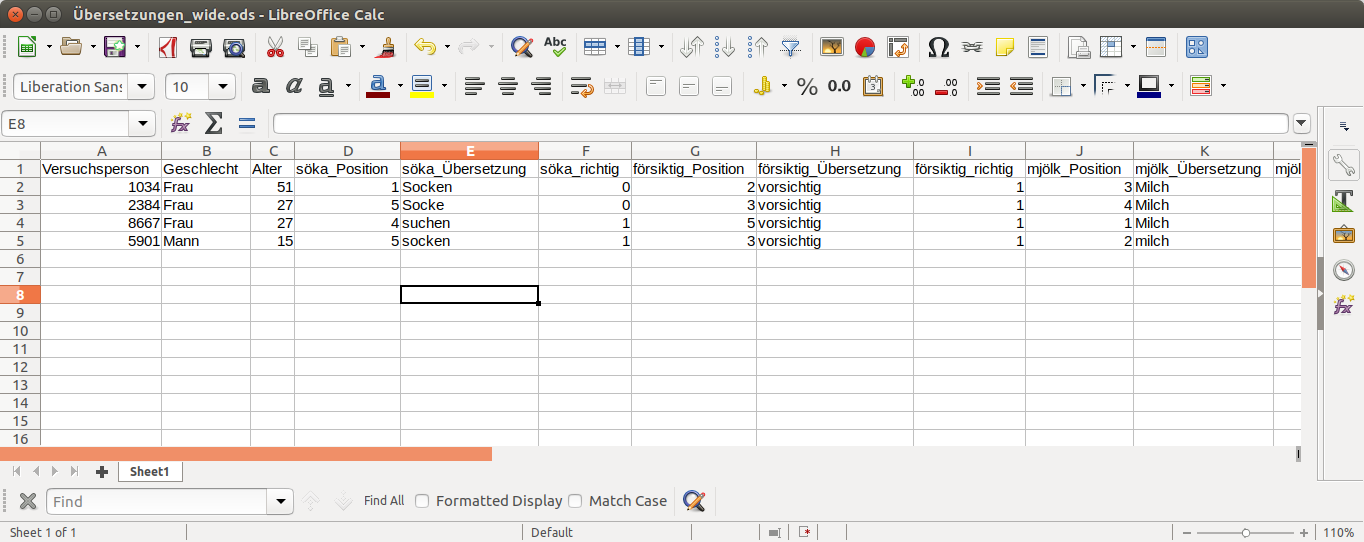
\includegraphics[width = \textwidth]{figs/wide_data_subject.png}
  \caption{A wide dataset with one row per participant.}
  \label{fig:wide_data_subject}
\end{figure}

\begin{figure}
  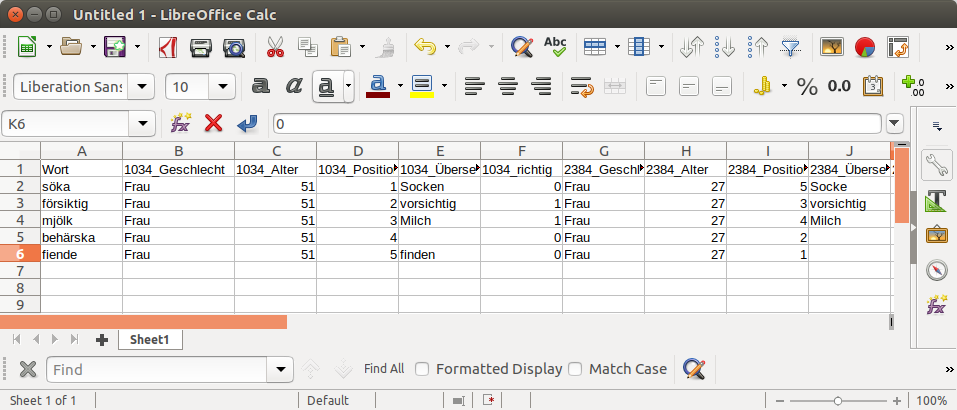
\includegraphics[width = \textwidth]{figs/wide_data_item.png}
  \caption{A wide dataset with one row per word.}
  \label{fig:wide_data_item}
\end{figure}

In a long format, all pieces of information pertaining to an \term{observational unit} 
are organised in a single row. 
It's difficult to precisely define what units of data collection and observational units are, 
and it wouldn't be too useful to have a precise definition, anyway. 
But in the present example, the observational units would be the individual responses, 
i.e., the individual translations. 
Figure \ref{fig:long_data} shows what the same data look like when organised in a long format.

\begin{figure}
  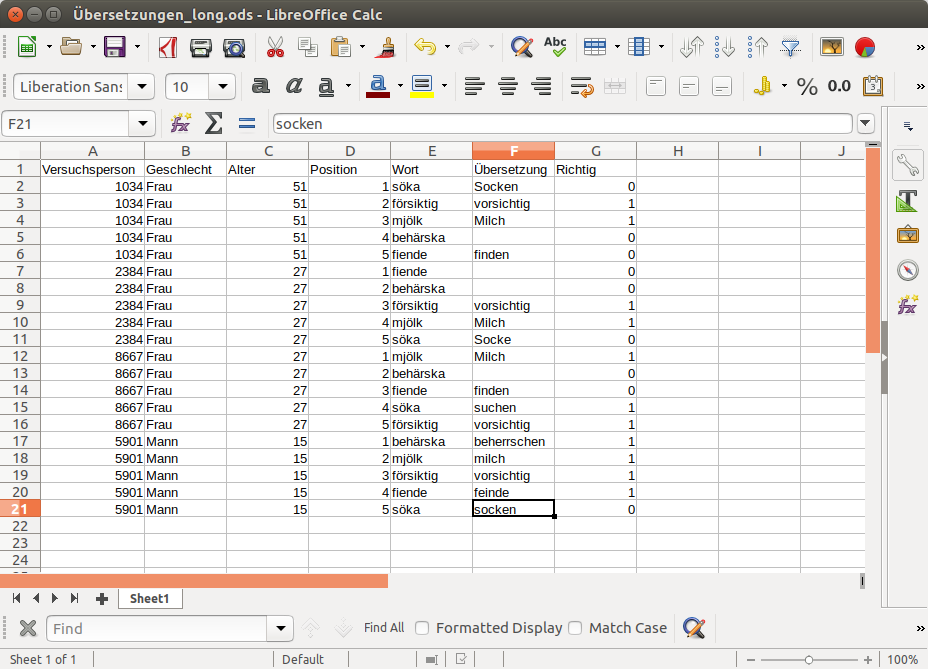
\includegraphics[width = \textwidth]{figs/long_data.png}
  \caption{A long dataset with one row per word per participant. Long datasets tend to be easier to manage and to analyse than wide ones.} 
  \label{fig:long_data}
\end{figure}

It's usually easier to work with data in a long-ish format compared to
data in a wide-ish format. 
Moreover, when you do need your data in a wide-ish format for a particular analysis, 
converting a longer dataset to a wider one is typically easier than vice versa.
We will, of course, illustrate how you can carry out such conversions.

\mypar{Tip}
  When in doubt, arrange your data in a long-ish format.
\parend

Make sure that all rows can be interpreted independently of one another.
What we want to avoid is that we can't make sense of the data in some row
because we need data from another row to do so, and this other row was
deleted, or the order of the rows has changed, etc.
For instance, in Figure \ref{fig:long_data}, we also have a column with the \texttt{Position}s,
even though we could have derived this information from the ordering of the rows.
But once a row gets deleted or once the order of the rows gets permuted,
we'd lose this piece of information.
So don't organise the data like in Figure \ref{fig:leere_zellen}.

\begin{figure}
  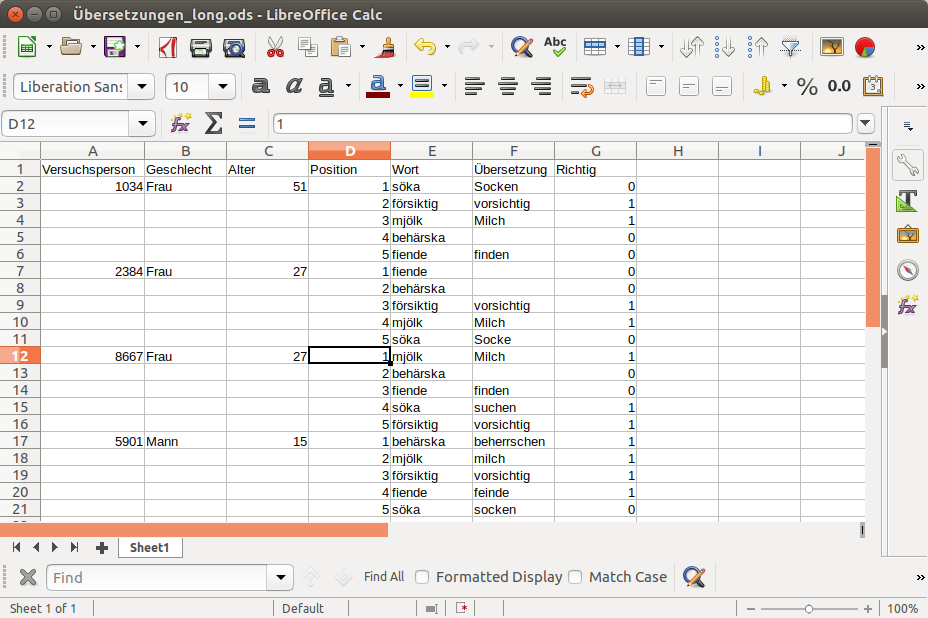
\includegraphics[width = \textwidth]{figs/long_data_nicht_so.png}
  \caption{Not like this! In this dataset, several cells are left empty as their contents can be derived from other cells. But this will result in difficulties when analysing the data. Moreover, deleting some rows or changing their order would make it impossible to reconstruct the intended contents of these empty cells.}
  \label{fig:leere_zellen}
\end{figure}

Furthermore, the dataset needs to be rectangular.
Figure \ref{fig:berechnungen_im_Spreadsheet} shows what \emph{not} to do: 
The additional rows reporting
some averages don't fit in with the rest of the dataset 
(``Prozent Männer:'' is not the ID of a \texttt{Versuchsperson}, 
and ``30'' is not a \texttt{Geschlecht}).

\begin{figure}
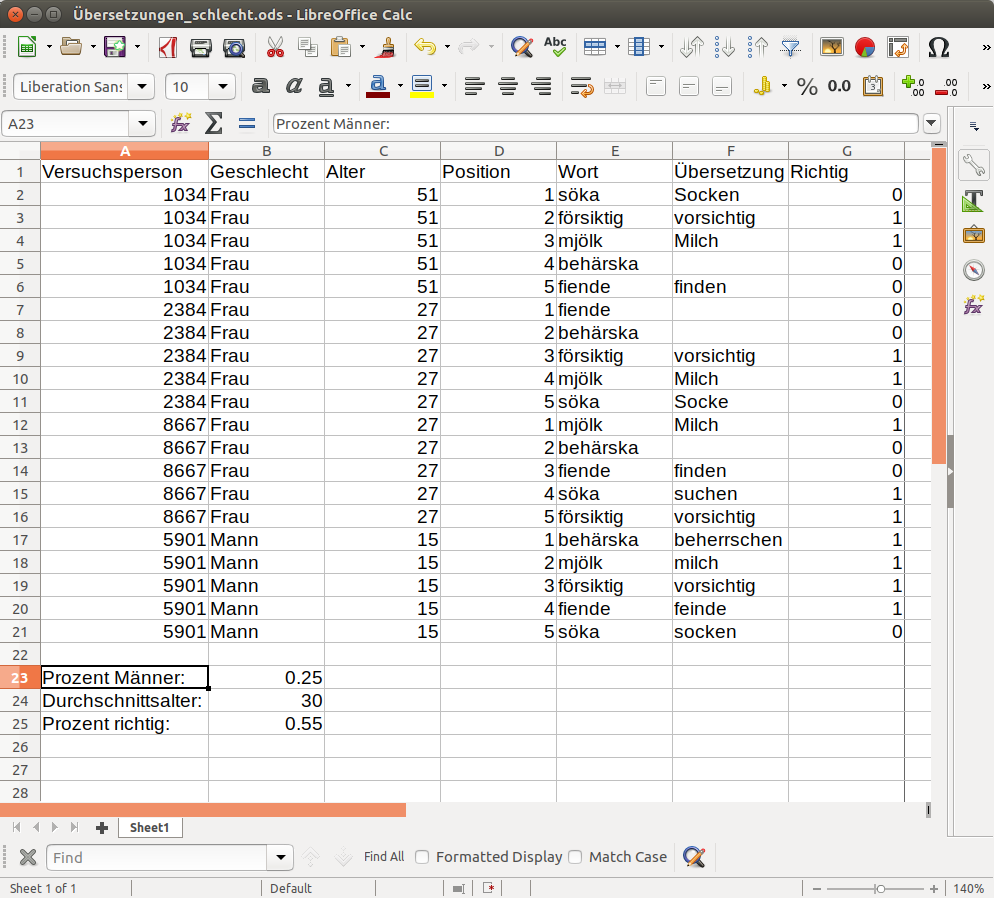
\includegraphics[width = \textwidth]{figs/datensatz_schlecht.png}
\caption{Not like this! This dataset is not rectangular.}
\label{fig:berechnungen_im_Spreadsheet}
\end{figure}

\subsection{Naming variables}
Make your life during the data analysis easier by using 
short but descriptive labels for variables or values in the spreadsheet.
By doing so, you avoid that you constantly need to look up in the project's codebook 
what the labels mean, thereby reducing the likelihood that you'll make errors.
Moreover, you save yourself some typing.

A few examples:
\begin{itemize}
  \item When working with questionnaire data, don't simply label the columns with the
        number of the question in the questionnaire (e.g., \texttt{Q3} or \texttt{Question17}).
        Instead, use more descriptive labels such as \texttt{DegreeFather} or \texttt{DialectUse}.
  \item If you have a column labelled \texttt{Sex} that is filled with 1s and 0s, 
        you'll constantly have to look up if the 1s refer to men or to women. 
        Instead, either fill the column with \texttt{m(an)} and \texttt{w(oman)} values, 
        or rename the column \texttt{Man}, 
        so that you know that the 1s refer to men.
  \item Try to strike a balance between descriptive power and length. 
        For instance, a variable named \texttt{HowOftenDoYouSpeakStandardGerman} 
        will get on your nerves before long; \texttt{SpeakStandard} could be sufficient.
\end{itemize}

\mypar[Use a codebook]{Tip}
  Having short and descriptive variable names is not an excuse for not maintaining  
  a codebook that spells out precisely what each variable in the dataset refers to.
  See \url{https://osf.io/d9gnh} for an example of a codebook.
\parend
 
\subsection{Labelling missing values}
In Figure \ref{fig:long_data}, I left some of the translation cells empty.
From this, I can deduce that the word was presented to the participant
but that he or she did not translate the word.
However, in other situations, it could be the case that some participants were inadvertently 
never shown a particular word (e.g., due to a programming error)
or that some of the participants' answers were irretrievably lost.
We should enable ourselves to distinguish between these cases, 
for instance by marking the latter cases using \texttt{NA} (\textit{not available}).
Alternatively, we could explicitly label cases where the participant did
not translate the word with \texttt{[no response]} or something similar.

If you want to be able to tell apart different reasons for missing data
(such as data loss, programming errors, participants' refusal to answer a certain
question, participants' being absent from a data collection etc.),
it's probably easiest to just write \texttt{NA} in the column and add another column
with comments detailing the reasons for the missingness.

Be aware that some data logging applications use $-99$ or $-9999$ to encode missingness.
The problem with this is that, sometimes, 
$-99$ or $-9999$ don't immediately stand out as conspicuous values.

\subsection{Using several smaller datasets}
The spreadsheet above contains several repeated pieces of information.
For instance, for all five translations provided by participant 1034,
we indicated that they were provided by a woman aged 51.
We can eliminate this source of redundancy by managing a handful
of smaller datasets rather than just a single large one.
More specifically, we can manage a dataset that contains all information
that depends \emph{just} on the participants, 
see Figure \ref{fig:versuchspersonen}.
Each participant has a unique ID (here: \texttt{Versuchsperson}),
and the dataset contains contains a single row for each participant.
If we need to correct an entry related to, say, some participant's age,
we just need to change it here---once---rather than five times in
the larger dataset.

\begin{figure}
  \centering
  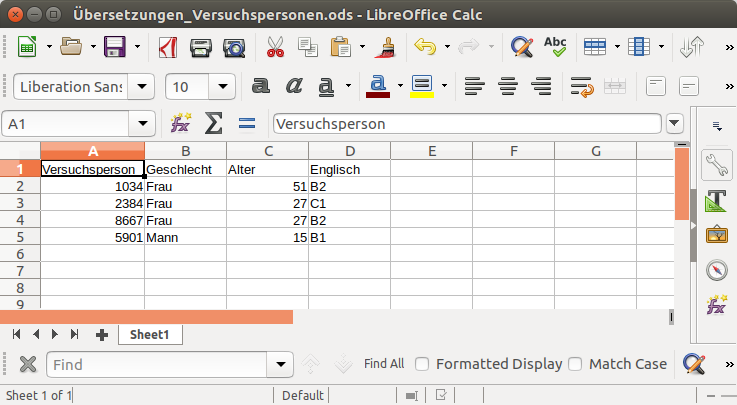
\includegraphics[width = 0.7\textwidth]{figs/versuchspersonen.png}
  \caption{The first smaller dataset only contains information concerning the participants.}
  \label{fig:versuchspersonen}
\end{figure}

By the same token, we can put all information that depends \emph{just}
on the stimuli used in a separate dataset, see Figure \ref{fig:woerter}.
Here, too, each stimulus has a unique ID (here: \texttt{Wort}).

\begin{figure}
  \centering
  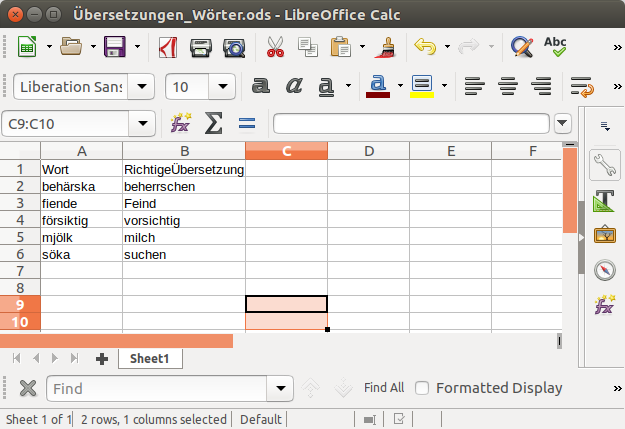
\includegraphics[width = 0.7\textwidth]{figs/woerter.png}
  \caption{The second smaller dataset only contains information concerning the words.}
  \label{fig:woerter}
\end{figure}

The third dataset then only contains information that depends
on the \emph{combination} of a particular participant and a particular word.
As shown in Figure \ref{fig:uebersetzungen}, each row in this dataset contains
the IDs of both the participant and the stimulus that the response is related to.
But any other information related to just the word or to just the participant
is left out of this dataset.
As we'll see shortly, we can easily add the information related to the participants
or to the words to this dataset from the other two datasets.

\begin{figure}
  \centering
  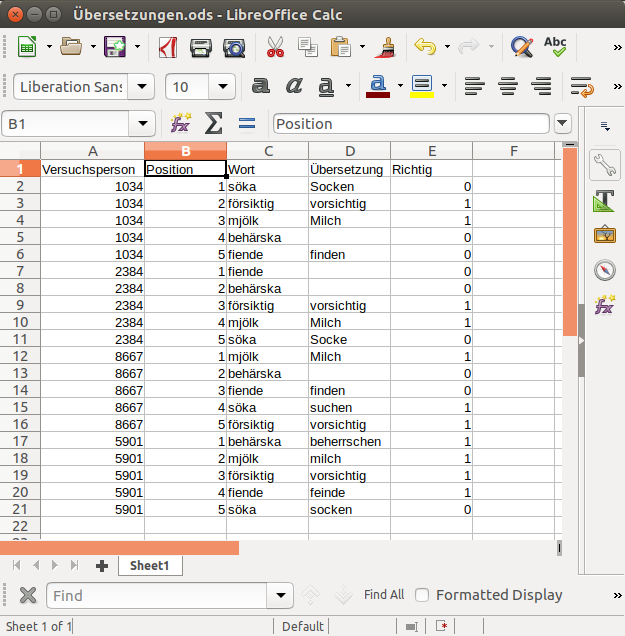
\includegraphics[width = 0.7\textwidth]{figs/uebersetzungen.png}
  \caption{The third dataset only contains the translations.}
  \label{fig:uebersetzungen}
\end{figure}

\subsection{Miscellaneous tips}
\begin{itemize}
  \item Mind capitalisation. 
        For some programs and computer languages (e.g., SQL), \texttt{Frau} and \texttt{frau}
        are the same value; for others (including R), they are not.
  \item Mind trailing spaces. \texttt{Mann␣} (with a trailing space) and \texttt{Mann} 
        (without a trailing space) are different values to a computer.
  \item Special symbols, including the Umlaut, sometimes lead to problems, especially when
        collaborating with people whose localisation settings differ from yours.
  \item Format dates in the YYYY/MM/DD format. 
        This way, if you sort the data alphabetically, they're already in chronological order.
  \item Don't use colour-coding in your spreadsheet. 
        Or if you do use it, be aware that you'll lose this information 
        once you import your data into your statistics program.
  \item Work as little as possible in the spreadsheet.
        After you've entered your data into a spreadsheet, all further steps in 
        your analysis should be carried out in R (or Python, or Julia, or what-have-you).
        Don't calculate, sort, copy, paste, move, reshape, draw graphs etc.\ in 
        Excel or whatever spreadsheet program you prefer. 
        Treat your finished spreadsheet as the \emph{immutable} source of data from which
        your results will be obtained, so that when in doubt, it's clear which 
        file you should go back to.

        When using R (or Python, or Julia, or whatever), use (a) script(s) to read in
        the original dataset and convert the data in it to a format more amenable to
        analysis, but whatever you do, don't overwrite the original file.

  \item Use data validation.
        When entering data in a spreadsheet program, you can use the data validation functions
        to minimise the chances that you enter faulty data. For instance, if you know
        that the possible responses to a certain question are either integers from
        0 to 5 or \texttt{NA},
        make a data validation rule that prevents you from entering impossible data.

        Also see the blog post 
        \href{https://janhove.github.io/posts/2018-07-06-data-entry-failsafes/}{\textit{A data entry form with failsafes}} 
        (6 July 2018).
\end{itemize}

\section{Reading in datasets}
We'll work with the \texttt{here} and \texttt{tidyverse} packages 
you've installed in the previous chapter.
Even if you've already installed these, you still need to \emph{load} 
these packages in every R session in which you use them. 
To do so, include the following lines in your R script and execute them:

\begin{knitrout}
\definecolor{shadecolor}{rgb}{0.969, 0.969, 0.969}\color{fgcolor}\begin{kframe}
\begin{alltt}
\hlkwd{library}\hldef{(here)}
\hlkwd{library}\hldef{(tidyverse)}
\end{alltt}
\end{kframe}
\end{knitrout}

If you run these commands, they will output a few messages.
The output of \texttt{library(here)} tells you the path relative to which
the \texttt{here()} function in the \texttt{here} package will look for files etc.
The messages generated by the \texttt{library(tidyverse)} command tell you 
which of the packages that make up the tidyverse suite are loaded by default.
Some of the functions in these packages have the same name as functions
that are part of packages that are loaded automatically whenever you start up
R. 
What this means is that, if you want to use, say, the \texttt{filter()} function
from the \texttt{stats} package, 
you need to use the notation \texttt{stats::filter()} 
instead of just \texttt{filter()}.

Incidentally, you don't need to install these packages every time you need them,
but you do need to load them every time you need them in a new session.
I recommend including all of the packages you need in a script at the top
of your script.
This way, everyone reading your script knows at the outset which packages they'll
have to install to reproduce your analysis.
Remove any \texttt{library()} commands for packages you ended up  not using in the script.

With all that out of the way, let's get started.
We'll focus on reading in two kinds of spreadsheets:
Excel spreadsheets in the XLS(X) format, and CSV files.

\subsection{Excel files}
In order to read in XLS(X) files, we need the \texttt{readxl} package.
This package is part of the \texttt{tidyverse} suite, but it does not get loaded
automatically as you load the \texttt{tidyverse} suite. So we load it separately:

\begin{knitrout}
\definecolor{shadecolor}{rgb}{0.969, 0.969, 0.969}\color{fgcolor}\begin{kframe}
\begin{alltt}
\hlkwd{library}\hldef{(readxl)}
\end{alltt}
\end{kframe}
\end{knitrout}

Assuming the file \texttt{uebersetzungen.xlsx} is located in the \texttt{data} 
subdirectory of your R project directory, we can read it into R as follows.

\begin{knitrout}
\definecolor{shadecolor}{rgb}{0.969, 0.969, 0.969}\color{fgcolor}\begin{kframe}
\begin{alltt}
\hldef{translations} \hlkwb{<-} \hlkwd{read_excel}\hldef{(}\hlkwd{here}\hldef{(}\hlsng{"data"}\hldef{,} \hlsng{"uebersetzungen.xlsx"}\hldef{))}
\end{alltt}
\end{kframe}
\end{knitrout}

The dataset is now loaded as a so-called \emph{tibble} named \texttt{translations}.
We can display it by simply typing its name at the prompt:
\begin{knitrout}
\definecolor{shadecolor}{rgb}{0.969, 0.969, 0.969}\color{fgcolor}\begin{kframe}
\begin{alltt}
\hldef{translations}
\end{alltt}
\begin{verbatim}
# A tibble: 20 x 5
  Versuchsperson Position Wort      Übersetzung Richtig
           <dbl>    <dbl> <chr>     <chr>         <dbl>
1           1034        1 söka      Socken            0
2           1034        2 försiktig vorsichtig        1
3           1034        3 mjölk     Milch             1
4           1034        4 behärska  <NA>              0
5           1034        5 fiende    finden            0
6           2384        1 fiende    <NA>              0
7           2384        2 behärska  <NA>              0
# i 13 more rows
\end{verbatim}
\end{kframe}
\end{knitrout}

\mypar[Type, don't copy-paste---at home]{Tip}
  You're going to take away much more from this course
  if you copy the code snippets by \emph{typing} them rather
  than by copy-pasting them.
  Do this at home and not during the lecture as you'll inevitably
  make some typos, causing you to lose track of the lecture.
\parend

\mypar[Assignment operators]{Remark}
  The symbol combination \texttt{<-} is the \textit{assignment operator}.
  It creates a new object in the working memory or overwrites an existing
  one with the same name.
  This object is referred to by the name to the left of the assignment
  operator.
  
  You'll often see that the equality sign (\texttt{=}) is used as
  the assignment operator.
  But it is also used to assign values to function parameters.
  I've tried to adhere to the \textit{one form, one function}
  principle throughout and only use \texttt{<-} as the assignment operator.
\parend

\mypar[Data frames and tibbles]{Remark}
  Rectangular data sets are referred to as \textit{data frames} in R.
  The \texttt{tidyverse} slightly changes their functionality, 
  mostly in order to allow for prettier displaying, and refers to them as \textit{tibbles}.
\parend

\mypar{Remark}
  Empty cells (for instance, the \texttt{Übersetzung} value in the fourth row) 
  are automatically interpreted as missing data (\texttt{<NA>}).
  The documentation of the \texttt{read\_excel()} function, 
  which you can access by typing \texttt{?read\_excel} at the R prompt, 
  suggests that we can override this behaviour,
  but \href{https://github.com/tidyverse/readxl/issues/572}{we can't}.
\parend

If, instead of printing the entire tibble at the prompt, 
we just want to display the first few rows, we can use \texttt{slide\_head()}:
\begin{knitrout}
\definecolor{shadecolor}{rgb}{0.969, 0.969, 0.969}\color{fgcolor}\begin{kframe}
\begin{alltt}
\hlkwd{slice_head}\hldef{(translations,} \hlkwc{n} \hldef{=} \hlnum{4}\hldef{)}
\end{alltt}
\begin{verbatim}
# A tibble: 4 x 5
  Versuchsperson Position Wort      Übersetzung Richtig
           <dbl>    <dbl> <chr>     <chr>         <dbl>
1           1034        1 söka      Socken            0
2           1034        2 försiktig vorsichtig        1
3           1034        3 mjölk     Milch             1
4           1034        4 behärska  <NA>              0
\end{verbatim}
\end{kframe}
\end{knitrout}

\texttt{slice\_tail()} works similarly. 
If you want to display a random selection of rows, you can use \texttt{slice\_sample()}:
\begin{knitrout}
\definecolor{shadecolor}{rgb}{0.969, 0.969, 0.969}\color{fgcolor}\begin{kframe}
\begin{alltt}
\hlkwd{slice_sample}\hldef{(translations,} \hlkwc{n} \hldef{=} \hlnum{5}\hldef{)}
\end{alltt}
\begin{verbatim}
# A tibble: 5 x 5
  Versuchsperson Position Wort     Übersetzung Richtig
           <dbl>    <dbl> <chr>    <chr>         <dbl>
1           8667        3 fiende   finden            0
2           8667        2 behärska <NA>              0
3           1034        4 behärska <NA>              0
4           1034        1 söka     Socken            0
5           2384        2 behärska <NA>              0
\end{verbatim}
\end{kframe}
\end{knitrout}

Again, for details, you can check the documentation of these functions that is available
at \texttt{?slice\_head}.

\mypar{Exercise}
  The file \texttt{VanDenBroek2018.xlsx} contains the data from
  three experiments reported by \citet{VanDenBroek2018}.
  Using the \texttt{read\_xlsx()} function, read in the data from the second experiment.

  Hint: Inspect the Excel file and then consult 
  the help page of \texttt{read\_xlsx()} by means of \texttt{?read\_xlsx}.
\parend

\subsection{CSV files}
A popular format for storing spreadsheets is the CSV format.
CSV is short for \textit{comma-separated values}:
Cells on the same row are separated by commas, see Figure \ref{fig:csv}.
Sometimes, text strings are additionally surrounded by quotation marks.

\begin{figure}
  \centering
  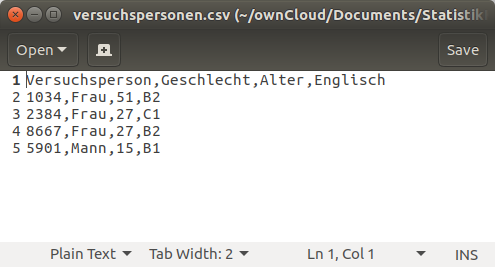
\includegraphics[width = 0.6\textwidth]{figs/csv.png}
  \caption{A spreadsheet stored as comma-separated values.}
  \label{fig:csv}
\end{figure}

To read in CSV files, we can use the \texttt{read\_csv()} function, 
which is part of the \texttt{readr} package, 
which in turn is automatically loaded when the \texttt{tidyverse} suit is loaded:

\begin{knitrout}
\definecolor{shadecolor}{rgb}{0.969, 0.969, 0.969}\color{fgcolor}\begin{kframe}
\begin{alltt}
\hldef{translations} \hlkwb{<-} \hlkwd{read_csv}\hldef{(}\hlkwd{here}\hldef{(}\hlsng{"data"}\hldef{,} \hlsng{"uebersetzungen.csv"}\hldef{))}
\hldef{translations}
\end{alltt}
\begin{verbatim}
# A tibble: 20 x 5
  Versuchsperson Position Wort      Übersetzung Richtig
           <dbl>    <dbl> <chr>     <chr>         <dbl>
1           1034        1 söka      Socken            0
2           1034        2 försiktig vorsichtig        1
3           1034        3 mjölk     Milch             1
4           1034        4 behärska  <NA>              0
5           1034        5 fiende    finden            0
6           2384        1 fiende    <NA>              0
7           2384        2 behärska  <NA>              0
# i 13 more rows
\end{verbatim}
\end{kframe}
\end{knitrout}

Running this command produces a number of messages,
which I haven't included in these lecture notes.
These messages show that the \texttt{read\_csv()} function correctly recognised that
the columns \texttt{Wort} and \texttt{Übersetzung} contain text (`chr', character) strings,
whereas \texttt{Versuchsperson}, \texttt{Position} and \texttt{Richtig} contain numbers
(`dbl' for `double', a number format).

\mypar{*Remark}
With \texttt{read\_csv()}, we can specify that only cells containing \texttt{NA} 
are marked as missing data:

\begin{knitrout}
\definecolor{shadecolor}{rgb}{0.969, 0.969, 0.969}\color{fgcolor}\begin{kframe}
\begin{alltt}
\hldef{translations2} \hlkwb{<-} \hlkwd{read_csv}\hldef{(}\hlkwd{here}\hldef{(}\hlsng{"data"}\hldef{,} \hlsng{"uebersetzungen.csv"}\hldef{),} \hlkwc{na} \hldef{=} \hlsng{"NA"}\hldef{)}
\hldef{translations2}
\end{alltt}
\begin{verbatim}
# A tibble: 20 x 5
  Versuchsperson Position Wort      Übersetzung  Richtig
           <dbl>    <dbl> <chr>     <chr>          <dbl>
1           1034        1 söka      "Socken"           0
2           1034        2 försiktig "vorsichtig"       1
3           1034        3 mjölk     "Milch"            1
4           1034        4 behärska  ""                 0
5           1034        5 fiende    "finden"           0
6           2384        1 fiende    ""                 0
7           2384        2 behärska  ""                 0
# i 13 more rows
\end{verbatim}
\end{kframe}
\end{knitrout}

Note that the \texttt{Übersetzung} value in row 4 is just empty, not \texttt{NA}.
\parend

Let's also read in the datasets containing the information pertaining
to the participants and items:

\begin{knitrout}
\definecolor{shadecolor}{rgb}{0.969, 0.969, 0.969}\color{fgcolor}\begin{kframe}
\begin{alltt}
\hldef{participants} \hlkwb{<-} \hlkwd{read_csv}\hldef{(}\hlkwd{here}\hldef{(}\hlsng{"data"}\hldef{,} \hlsng{"versuchspersonen.csv"}\hldef{))}
\hldef{items} \hlkwb{<-} \hlkwd{read_csv}\hldef{(}\hlkwd{here}\hldef{(}\hlsng{"data"}\hldef{,} \hlsng{"woerter.csv"}\hldef{))}
\end{alltt}
\end{kframe}
\end{knitrout}

\mypar[Different CSV formats]{Remark}
  If you save an Excel spreadsheet as a CSV file on a French- or German-language
  computer system, the cells will be separated using semicolons rather than using
  commas. The reason is that commas are used as decimal separators in French
  and German. To read in `CSV' files that use semicolons as cell separators,
  you can use the \texttt{read\_csv2()} function.
  
  Incidentally, if you use 
  \href{https://www.libreoffice.org/}{LibreOffice.org Calc} instead of Excel, 
  you can choose which cell separator gets used 
  if you export a spreadsheet as a CSV file.
\parend

\mypar[*\texttt{read\_csv()} vs.\ \texttt{read.csv()}]{Remark}
  More seasoned R users are probably already familiar with the \texttt{read.csv()} function
  (with a dot rather than an underscore). 
  The \texttt{read\_csv()} function is merely the
  tidyverse counterpart to this function.
  The main difference between them is that \texttt{read\_csv()} creates
  tibbles, whereas \texttt{read.csv()} creates dataframes.
\parend


\subsection{Other formats}
Some people prefer to use tabs or spaces to separate cells rather than commas or semicolons.
Consult the help page for the \texttt{read\_tsv()} and \texttt{read\_delim()} functions 
to see how you can read in data using other separators. 
Particularly the \texttt{delim} and \texttt{quote} arguments are relevant.

For reading in data from Google Sheets, see \href{https://googlesheets4.tidyverse.org/}{\texttt{googlesheets4}}.

For interacting with Google Drive, see \href{https://googledrive.tidyverse.org/}{\texttt{googledrive}}.

For reading in SPSS, Stata and SAS files, see \href{https://haven.tidyverse.org}{\texttt{haven}}.

\section{Joining datasets}
Having read in our three datasets as 
\texttt{translations}, \texttt{participants}, and \texttt{items},
we want to merge these datasets into one large dataset. 
The most useful function for this is \texttt{left\_join()}, 
which takes the dataset passed as its \texttt{x} argument
and adds to this the corresponding rows from the \texttt{y} dataset:
\begin{knitrout}
\definecolor{shadecolor}{rgb}{0.969, 0.969, 0.969}\color{fgcolor}\begin{kframe}
\begin{alltt}
\hldef{all_data} \hlkwb{<-} \hlkwd{left_join}\hldef{(}\hlkwc{x} \hldef{= translations,} \hlkwc{y} \hldef{= participants)}
\end{alltt}
\end{kframe}
\end{knitrout}

Note that the \texttt{left\_join()} function recognises that the variable shared
between both datasets is called \texttt{Versuchsperson}. 
Hence, the information related to participant 1034 
contained in \texttt{participants} is added to each row in 
\texttt{translations} for which the value of \texttt{Versuchsperson} is 1034,
and similarly for the other participants:
\begin{knitrout}
\definecolor{shadecolor}{rgb}{0.969, 0.969, 0.969}\color{fgcolor}\begin{kframe}
\begin{alltt}
\hldef{all_data}
\end{alltt}
\begin{verbatim}
# A tibble: 20 x 8
  Versuchsperson Position Wort      Übersetzung Richtig
           <dbl>    <dbl> <chr>     <chr>         <dbl>
1           1034        1 söka      Socken            0
2           1034        2 försiktig vorsichtig        1
3           1034        3 mjölk     Milch             1
4           1034        4 behärska  <NA>              0
5           1034        5 fiende    finden            0
6           2384        1 fiende    <NA>              0
7           2384        2 behärska  <NA>              0
# i 13 more rows
# i 3 more variables: Geschlecht <chr>, Alter <dbl>,
#   Englisch <chr>
\end{verbatim}
\end{kframe}
\end{knitrout}

If you don't want the \texttt{left\_join()} function to figure out 
what the shared variable is, you can specify it explicitly:
\begin{knitrout}
\definecolor{shadecolor}{rgb}{0.969, 0.969, 0.969}\color{fgcolor}\begin{kframe}
\begin{alltt}
\hldef{all_data} \hlkwb{<-} \hlkwd{left_join}\hldef{(}\hlkwc{x} \hldef{= translations,} \hlkwc{y} \hldef{= participants,}
                      \hlkwc{by} \hldef{=} \hlsng{"Versuchsperson"}\hldef{)}
\end{alltt}
\end{kframe}
\end{knitrout}

If the shared variable has different names in the different datasets, 
you can use something like
\begin{knitrout}
\definecolor{shadecolor}{rgb}{0.969, 0.969, 0.969}\color{fgcolor}\begin{kframe}
\begin{alltt}
\hldef{new} \hlkwb{<-} \hlkwd{left_join}\hldef{(}\hlkwc{x} \hldef{= left_dataset,} \hlkwc{y} \hldef{= right_dataset,}
                 \hlkwc{by} \hldef{=} \hlkwd{join_by}\hldef{(var_left} \hlopt{==} \hldef{var_right))}
\end{alltt}
\end{kframe}
\end{knitrout}
See \texttt{?join\_by} for more information.

If there are values in the shared variable that occur in the \texttt{x} dataset
that don't occur in the \texttt{y} dataset, 
the values in the added columns will read \texttt{NA} for these rows.

Further join functions are the following, see \texttt{?join} for details:
\begin{itemize}
  \item \texttt{right\_join(x, y)}: Keep all entries in \texttt{y}. 
        Add corresponding entries in \texttt{x} to it.
        
  \item \texttt{full\_join(x, y)}: Keep all entries in both \texttt{x} and \texttt{y}. 
        Add \texttt{NA}s if there is no corresponding entry in the other dataset.
        
  \item \texttt{inner\_join(x, y)}: Only keep entries in \texttt{x} for which
         there is a corresponding entry in \texttt{y}. Add these corresponding entries.

  \item \texttt{semi\_join(x, y)}:  Only keep entries in \texttt{x} for which 
         there is a corresponding entry in \texttt{y}. Don't add these corresponding entries.

  \item \texttt{anti\_join(x, y)}: Only keep entries in \texttt{x} for which 
         there are \emph{no} corresponding entries in \texttt{y}.
\end{itemize}

In the current example, \texttt{left\_join()}, \texttt{full\_join()} and 
\texttt{inner\_join()} would all yield the same result.
But this isn't always the case.

Let's also add the information pertaining to the words:
\begin{knitrout}
\definecolor{shadecolor}{rgb}{0.969, 0.969, 0.969}\color{fgcolor}\begin{kframe}
\begin{alltt}
\hldef{all_data} \hlkwb{<-} \hlkwd{left_join}\hldef{(all_data, items)}
\end{alltt}
\end{kframe}
\end{knitrout}

\mypar[Join functions]{Exercise}
\begin{enumerate}
  \item Use the following code to generate two tibbles called \texttt{left} and \texttt{right},
        and to inspect them:
\begin{knitrout}
\definecolor{shadecolor}{rgb}{0.969, 0.969, 0.969}\color{fgcolor}\begin{kframe}
\begin{alltt}
\hldef{left} \hlkwb{<-} \hlkwd{tibble}\hldef{(}\hlkwc{A} \hldef{=} \hlkwd{c}\hldef{(}\hlsng{"a"}\hldef{,} \hlsng{"b"}\hldef{,} \hlsng{"c"}\hldef{,} \hlnum{NA}\hldef{),}
               \hlkwc{B} \hldef{=} \hlkwd{c}\hldef{(}\hlnum{1}\hldef{,} \hlnum{2}\hldef{,} \hlnum{NA}\hldef{,} \hlnum{4}\hldef{))}
\hldef{right} \hlkwb{<-} \hlkwd{tibble}\hldef{(}\hlkwc{B} \hldef{=} \hlkwd{c}\hldef{(}\hlnum{1}\hldef{,} \hlnum{3}\hldef{,} \hlnum{4}\hldef{,} \hlnum{4}\hldef{),}
                \hlkwc{C} \hldef{=} \hlkwd{c}\hldef{(}\hlnum{10}\hldef{,} \hlnum{NA}\hldef{,} \hlnum{12}\hldef{,} \hlnum{7}\hldef{))}
\hldef{left}
\hldef{right}
\end{alltt}
\end{kframe}
\end{knitrout}

  \item \emph{Without running the following commands}, 
        predict what their output will look like:
\begin{knitrout}
\definecolor{shadecolor}{rgb}{0.969, 0.969, 0.969}\color{fgcolor}\begin{kframe}
\begin{alltt}
\hlkwd{left_join}\hldef{(}\hlkwc{x} \hldef{= left,} \hlkwc{y} \hldef{= right)}
\hlkwd{right_join}\hldef{(}\hlkwc{x} \hldef{= left,} \hlkwc{y} \hldef{= right)}
\hlkwd{full_join}\hldef{(}\hlkwc{x} \hldef{= left,} \hlkwc{y} \hldef{= right)}
\hlkwd{inner_join}\hldef{(}\hlkwc{x} \hldef{= left,} \hlkwc{y} \hldef{= right)}
\hlkwd{semi_join}\hldef{(}\hlkwc{x} \hldef{= left,} \hlkwc{y} \hldef{= right)}
\hlkwd{semi_join}\hldef{(}\hlkwc{x} \hldef{= right,} \hlkwc{y} \hldef{= left)} \hlcom{# !}
\hlkwd{anti_join}\hldef{(}\hlkwc{x} \hldef{= left,} \hlkwc{y} \hldef{= right)}
\hlkwd{anti_join}\hldef{(}\hlkwc{x} \hldef{= right,} \hlkwc{y} \hldef{= left)} \hlcom{# !}
\end{alltt}
\end{kframe}
\end{knitrout}
        
  \item Now run the commands above to verify your predictions.

  \item Create two new tibbles using the code below:
\begin{knitrout}
\definecolor{shadecolor}{rgb}{0.969, 0.969, 0.969}\color{fgcolor}\begin{kframe}
\begin{alltt}
\hldef{left} \hlkwb{<-} \hlkwd{tibble}\hldef{(}\hlkwc{A} \hldef{=} \hlkwd{c}\hldef{(}\hlsng{"a"}\hldef{,} \hlsng{"b"}\hldef{),}
               \hlkwc{B} \hldef{=} \hlkwd{c}\hldef{(}\hlnum{1}\hldef{,} \hlnum{NA}\hldef{))}
\hldef{right} \hlkwb{<-} \hlkwd{tibble}\hldef{(}\hlkwc{B} \hldef{=} \hlkwd{c}\hldef{(}\hlnum{1}\hldef{,} \hlnum{NA}\hldef{,} \hlnum{NA}\hldef{),}
                \hlkwc{C} \hldef{=} \hlkwd{c}\hldef{(}\hlnum{0}\hldef{,} \hlnum{1}\hldef{,} \hlnum{2}\hldef{))}
\hldef{left}
\hldef{right}
\end{alltt}
\end{kframe}
\end{knitrout}

  \item Consult the help page for \texttt{left\_join()} and look up the \texttt{na\_matches}
        parameter under `Arguments'. 
        Predict what the output of the following two commands will look like,
        and only then check your answer.
\begin{knitrout}
\definecolor{shadecolor}{rgb}{0.969, 0.969, 0.969}\color{fgcolor}\begin{kframe}
\begin{alltt}
\hlkwd{left_join}\hldef{(left, right)}
\hlkwd{left_join}\hldef{(left, right,} \hlkwc{na_matches} \hldef{=} \hlsng{"never"}\hldef{)}
\end{alltt}
\end{kframe}
\end{knitrout}
\parend
\end{enumerate}

\section{Queries}
\subsection{Selecting by row number}
We can select the third row of a dataset like so:
\begin{knitrout}
\definecolor{shadecolor}{rgb}{0.969, 0.969, 0.969}\color{fgcolor}\begin{kframe}
\begin{alltt}
\hlkwd{slice}\hldef{(all_data,} \hlnum{3}\hldef{)}
\end{alltt}
\begin{verbatim}
# A tibble: 1 x 9
  Versuchsperson Position Wort  Übersetzung Richtig
           <dbl>    <dbl> <chr> <chr>         <dbl>
1           1034        3 mjölk Milch             1
# i 4 more variables: Geschlecht <chr>, Alter <dbl>,
#   Englisch <chr>, RichtigeÜbersetzung <chr>
\end{verbatim}
\end{kframe}
\end{knitrout}

Alternatively, we can write this command as follows.
The symbol combination \texttt{|>} allows us to take an object 
(here: \texttt{all\_data})
and pass it to a function as its first argument.
As we'll later see, we can use \texttt{|>} to string together a host of function calls
without creating illegible code.
\begin{knitrout}
\definecolor{shadecolor}{rgb}{0.969, 0.969, 0.969}\color{fgcolor}\begin{kframe}
\begin{alltt}
\hldef{all_data |>}
  \hlkwd{slice}\hldef{(}\hlnum{3}\hldef{)}
\end{alltt}
\begin{verbatim}
# A tibble: 1 x 9
  Versuchsperson Position Wort  Übersetzung Richtig
           <dbl>    <dbl> <chr> <chr>         <dbl>
1           1034        3 mjölk Milch             1
# i 4 more variables: Geschlecht <chr>, Alter <dbl>,
#   Englisch <chr>, RichtigeÜbersetzung <chr>
\end{verbatim}
\end{kframe}
\end{knitrout}
Use \textsc{ctrl + shift + m} (Windows, Linux) or \textsc{cmd + shift + m} (macOS)
to insert \texttt{|>} at the current text cursor position.

We can also select multiple rows:
\begin{knitrout}
\definecolor{shadecolor}{rgb}{0.969, 0.969, 0.969}\color{fgcolor}\begin{kframe}
\begin{alltt}
\hlcom{# Rows 5 and 7}
\hldef{all_data |>}
  \hlkwd{slice}\hldef{(}\hlkwd{c}\hldef{(}\hlnum{5}\hldef{,} \hlnum{7}\hldef{))}
\end{alltt}
\begin{verbatim}
# A tibble: 2 x 9
  Versuchsperson Position Wort     Übersetzung Richtig
           <dbl>    <dbl> <chr>    <chr>         <dbl>
1           1034        5 fiende   finden            0
2           2384        2 behärska <NA>              0
# i 4 more variables: Geschlecht <chr>, Alter <dbl>,
#   Englisch <chr>, RichtigeÜbersetzung <chr>
\end{verbatim}
\begin{alltt}
\hlcom{# Rows 5 to (and including) 7}
\hldef{all_data |>}
  \hlkwd{slice}\hldef{(}\hlnum{5}\hlopt{:}\hlnum{7}\hldef{)}
\end{alltt}
\begin{verbatim}
# A tibble: 3 x 9
  Versuchsperson Position Wort     Übersetzung Richtig
           <dbl>    <dbl> <chr>    <chr>         <dbl>
1           1034        5 fiende   finden            0
2           2384        1 fiende   <NA>              0
3           2384        2 behärska <NA>              0
# i 4 more variables: Geschlecht <chr>, Alter <dbl>,
#   Englisch <chr>, RichtigeÜbersetzung <chr>
\end{verbatim}
\end{kframe}
\end{knitrout}

The results of such actions can be stored as separate objects, for instance, like so:
\begin{knitrout}
\definecolor{shadecolor}{rgb}{0.969, 0.969, 0.969}\color{fgcolor}\begin{kframe}
\begin{alltt}
\hldef{rows7_12} \hlkwb{<-} \hldef{all_data |>}
  \hlkwd{slice}\hldef{(}\hlnum{7}\hlopt{:}\hlnum{12}\hldef{)}
\hldef{rows7_12}
\end{alltt}
\begin{verbatim}
# A tibble: 6 x 9
  Versuchsperson Position Wort      Übersetzung Richtig
           <dbl>    <dbl> <chr>     <chr>         <dbl>
1           2384        2 behärska  <NA>              0
2           2384        3 försiktig vorsichtig        1
3           2384        4 mjölk     Milch             1
4           2384        5 söka      Socke             0
5           8667        1 mjölk     Milch             1
6           8667        2 behärska  <NA>              0
# i 4 more variables: Geschlecht <chr>, Alter <dbl>,
#   Englisch <chr>, RichtigeÜbersetzung <chr>
\end{verbatim}
\end{kframe}
\end{knitrout}

We can export this new object as a CSV file like so:
\begin{knitrout}
\definecolor{shadecolor}{rgb}{0.969, 0.969, 0.969}\color{fgcolor}\begin{kframe}
\begin{alltt}
\hlkwd{write_csv}\hldef{(rows7_12,} \hlkwd{here}\hldef{(}\hlsng{"data"}\hldef{,} \hlsng{"rows7_12.csv"}\hldef{))}
\end{alltt}
\end{kframe}
\end{knitrout}

\subsection{Selecting rows by values}
Selecting rows by their number isn't too useful.
But selecting rows satisfying some set of conditions is very useful.
Here are a few examples:
\begin{knitrout}
\definecolor{shadecolor}{rgb}{0.969, 0.969, 0.969}\color{fgcolor}\begin{kframe}
\begin{alltt}
\hlcom{# All data corresponding to the word 'fiende'}
\hldef{all_data |>}
  \hlkwd{filter}\hldef{(Wort} \hlopt{==} \hlsng{"fiende"}\hldef{)}
\end{alltt}
\begin{verbatim}
# A tibble: 4 x 9
  Versuchsperson Position Wort   Übersetzung Richtig
           <dbl>    <dbl> <chr>  <chr>         <dbl>
1           1034        5 fiende finden            0
2           2384        1 fiende <NA>              0
3           8667        3 fiende finden            0
4           5901        4 fiende feinde            1
# i 4 more variables: Geschlecht <chr>, Alter <dbl>,
#   Englisch <chr>, RichtigeÜbersetzung <chr>
\end{verbatim}
\begin{alltt}
\hlcom{# Note: use '!=' for 'not equal to'.}

\hlcom{# All data corresponding to participants older than 30}
\hldef{all_data |>}
  \hlkwd{filter}\hldef{(Alter} \hlopt{>} \hlnum{30}\hldef{)}
\end{alltt}
\begin{verbatim}
# A tibble: 5 x 9
  Versuchsperson Position Wort      Übersetzung Richtig
           <dbl>    <dbl> <chr>     <chr>         <dbl>
1           1034        1 söka      Socken            0
2           1034        2 försiktig vorsichtig        1
3           1034        3 mjölk     Milch             1
4           1034        4 behärska  <NA>              0
5           1034        5 fiende    finden            0
# i 4 more variables: Geschlecht <chr>, Alter <dbl>,
#   Englisch <chr>, RichtigeÜbersetzung <chr>
\end{verbatim}
\begin{alltt}
\hlcom{# Note: use '>=' for 'at least as old as', }
\hlcom{#           '<=' for 'no older than', }
\hlcom{#        and '<' for 'younger than'.}
\end{alltt}
\end{kframe}
\end{knitrout}

We can use \texttt{is.na()} to check for missing values. 
Note the use of \texttt{!} to negate a condition.
\begin{knitrout}
\definecolor{shadecolor}{rgb}{0.969, 0.969, 0.969}\color{fgcolor}\begin{kframe}
\begin{alltt}
\hldef{all_data |>}
  \hlkwd{filter}\hldef{(}\hlkwd{is.na}\hldef{(Übersetzung))}
\end{alltt}
\begin{verbatim}
# A tibble: 4 x 9
  Versuchsperson Position Wort     Übersetzung Richtig
           <dbl>    <dbl> <chr>    <chr>         <dbl>
1           1034        4 behärska <NA>              0
2           2384        1 fiende   <NA>              0
3           2384        2 behärska <NA>              0
4           8667        2 behärska <NA>              0
# i 4 more variables: Geschlecht <chr>, Alter <dbl>,
#   Englisch <chr>, RichtigeÜbersetzung <chr>
\end{verbatim}
\begin{alltt}
\hldef{all_data |>}
  \hlkwd{filter}\hldef{(}\hlopt{!}\hlkwd{is.na}\hldef{(Übersetzung))}
\end{alltt}
\begin{verbatim}
# A tibble: 16 x 9
  Versuchsperson Position Wort      Übersetzung Richtig
           <dbl>    <dbl> <chr>     <chr>         <dbl>
1           1034        1 söka      Socken            0
2           1034        2 försiktig vorsichtig        1
3           1034        3 mjölk     Milch             1
4           1034        5 fiende    finden            0
5           2384        3 försiktig vorsichtig        1
6           2384        4 mjölk     Milch             1
7           2384        5 söka      Socke             0
# i 9 more rows
# i 4 more variables: Geschlecht <chr>, Alter <dbl>,
#   Englisch <chr>, RichtigeÜbersetzung <chr>
\end{verbatim}
\end{kframe}
\end{knitrout}

We can string together multiple \texttt{filter()} calls:
\begin{knitrout}
\definecolor{shadecolor}{rgb}{0.969, 0.969, 0.969}\color{fgcolor}\begin{kframe}
\begin{alltt}
\hlcom{# incorrect translations to first word}
\hldef{all_data |>}
  \hlkwd{filter}\hldef{(Position} \hlopt{==} \hlnum{1}\hldef{) |>}
  \hlkwd{filter}\hldef{(Richtig} \hlopt{==} \hlnum{0}\hldef{)}
\end{alltt}
\begin{verbatim}
# A tibble: 2 x 9
  Versuchsperson Position Wort   Übersetzung Richtig
           <dbl>    <dbl> <chr>  <chr>         <dbl>
1           1034        1 söka   Socken            0
2           2384        1 fiende <NA>              0
# i 4 more variables: Geschlecht <chr>, Alter <dbl>,
#   Englisch <chr>, RichtigeÜbersetzung <chr>
\end{verbatim}
\end{kframe}
\end{knitrout}

An alternative way of writing this is as follows:
\begin{knitrout}
\definecolor{shadecolor}{rgb}{0.969, 0.969, 0.969}\color{fgcolor}\begin{kframe}
\begin{alltt}
\hldef{all_data |>}
  \hlkwd{filter}\hldef{(Position} \hlopt{==} \hlnum{1} \hlopt{&} \hldef{Richtig} \hlopt{==} \hlnum{0}\hldef{)}
\end{alltt}
\begin{verbatim}
# A tibble: 2 x 9
  Versuchsperson Position Wort   Übersetzung Richtig
           <dbl>    <dbl> <chr>  <chr>         <dbl>
1           1034        1 söka   Socken            0
2           2384        1 fiende <NA>              0
# i 4 more variables: Geschlecht <chr>, Alter <dbl>,
#   Englisch <chr>, RichtigeÜbersetzung <chr>
\end{verbatim}
\end{kframe}
\end{knitrout}

`or' conditions can be created using \texttt{|}:
\begin{knitrout}
\definecolor{shadecolor}{rgb}{0.969, 0.969, 0.969}\color{fgcolor}\begin{kframe}
\begin{alltt}
\hlcom{# translations to first word or incorrect translations}
\hldef{all_data |>}
  \hlkwd{filter}\hldef{(Position} \hlopt{==} \hlnum{1} \hlopt{|} \hldef{Richtig} \hlopt{==} \hlnum{0}\hldef{)}
\end{alltt}
\begin{verbatim}
# A tibble: 11 x 9
  Versuchsperson Position Wort     Übersetzung Richtig
           <dbl>    <dbl> <chr>    <chr>         <dbl>
1           1034        1 söka     Socken            0
2           1034        4 behärska <NA>              0
3           1034        5 fiende   finden            0
4           2384        1 fiende   <NA>              0
5           2384        2 behärska <NA>              0
6           2384        5 söka     Socke             0
7           8667        1 mjölk    Milch             1
# i 4 more rows
# i 4 more variables: Geschlecht <chr>, Alter <dbl>,
#   Englisch <chr>, RichtigeÜbersetzung <chr>
\end{verbatim}
\end{kframe}
\end{knitrout}

Note that in logic, `or' is always inclusive.
Exclusive `or' (`xor') can be obtained as follows:
\begin{knitrout}
\definecolor{shadecolor}{rgb}{0.969, 0.969, 0.969}\color{fgcolor}\begin{kframe}
\begin{alltt}
\hlcom{# translations to first word or incorrect translations, but not both}
\hldef{all_data |>}
  \hlkwd{filter}\hldef{(Position} \hlopt{==} \hlnum{1} \hlopt{|} \hldef{Richtig} \hlopt{==} \hlnum{0}\hldef{) |>}
  \hlkwd{filter}\hldef{(}\hlopt{!}\hldef{(Position} \hlopt{==} \hlnum{1} \hlopt{&} \hldef{Richtig} \hlopt{==} \hlnum{0}\hldef{))}
\end{alltt}
\begin{verbatim}
# A tibble: 9 x 9
  Versuchsperson Position Wort     Übersetzung Richtig
           <dbl>    <dbl> <chr>    <chr>         <dbl>
1           1034        4 behärska <NA>              0
2           1034        5 fiende   finden            0
3           2384        2 behärska <NA>              0
4           2384        5 söka     Socke             0
5           8667        1 mjölk    Milch             1
6           8667        2 behärska <NA>              0
7           8667        3 fiende   finden            0
# i 2 more rows
# i 4 more variables: Geschlecht <chr>, Alter <dbl>,
#   Englisch <chr>, RichtigeÜbersetzung <chr>
\end{verbatim}
\end{kframe}
\end{knitrout}

Alternatively,
\begin{knitrout}
\definecolor{shadecolor}{rgb}{0.969, 0.969, 0.969}\color{fgcolor}\begin{kframe}
\begin{alltt}
\hldef{all_data |>}
  \hlkwd{filter}\hldef{(}\hlkwd{xor}\hldef{(Position} \hlopt{==} \hlnum{1}\hldef{, Richtig} \hlopt{==} \hlnum{0}\hldef{))}
\end{alltt}
\begin{verbatim}
# A tibble: 9 x 9
  Versuchsperson Position Wort     Übersetzung Richtig
           <dbl>    <dbl> <chr>    <chr>         <dbl>
1           1034        4 behärska <NA>              0
2           1034        5 fiende   finden            0
3           2384        2 behärska <NA>              0
4           2384        5 söka     Socke             0
5           8667        1 mjölk    Milch             1
6           8667        2 behärska <NA>              0
7           8667        3 fiende   finden            0
# i 2 more rows
# i 4 more variables: Geschlecht <chr>, Alter <dbl>,
#   Englisch <chr>, RichtigeÜbersetzung <chr>
\end{verbatim}
\end{kframe}
\end{knitrout}

\mypar[Filtering]{Exercise}
\begin{enumerate}
  \item Run the following commands:
\begin{knitrout}
\definecolor{shadecolor}{rgb}{0.969, 0.969, 0.969}\color{fgcolor}\begin{kframe}
\begin{alltt}
\hldef{d1} \hlkwb{<-} \hldef{all_data |>}
  \hlkwd{filter}\hldef{(Übersetzung} \hlopt{==} \hlsng{"vorsichtig"}\hldef{)}
\hldef{d2} \hlkwb{<-} \hldef{all_data |>}
  \hlkwd{filter}\hldef{(Übersetzung} \hlopt{!=} \hlsng{"vorsichtig"}\hldef{)}
\end{alltt}
\end{kframe}
\end{knitrout}

  \item Explain what both commands achieve.

  \item How many rows are there in \texttt{d1}? 
        How many in \texttt{d2}? 
        How many in \texttt{all\_data}?
        Explain.

  \item Create a tibble \texttt{d3} that contains only those rows in \texttt{all\_data} 
        where the participants did not translate the word as \textit{vorsichtig}.\parend
\end{enumerate}

\mypar[String detection]{Remark}
It is also possible to perform more complex string-based queries.
For instance, the \texttt{stringr} package, which is loaded automatically as part
of the tidyverse, contains the function \texttt{str\_detect()}. 
As its name suggests, this function can be used to detect if a string contains a 
particular combination of symbols:
\begin{knitrout}
\definecolor{shadecolor}{rgb}{0.969, 0.969, 0.969}\color{fgcolor}\begin{kframe}
\begin{alltt}
\hlcom{# all rows with an Übersetzung containing "ch"}
\hldef{all_data |>}
  \hlkwd{filter}\hldef{(}\hlkwd{str_detect}\hldef{(Übersetzung,} \hlsng{"ch"}\hldef{))}
\end{alltt}
\begin{verbatim}
# A tibble: 10 x 9
  Versuchsperson Position Wort      Übersetzung Richtig
           <dbl>    <dbl> <chr>     <chr>         <dbl>
1           1034        2 försiktig vorsichtig        1
2           1034        3 mjölk     Milch             1
3           2384        3 försiktig vorsichtig        1
4           2384        4 mjölk     Milch             1
5           8667        1 mjölk     Milch             1
6           8667        4 söka      suchen            1
7           8667        5 försiktig vorsichtig        1
# i 3 more rows
# i 4 more variables: Geschlecht <chr>, Alter <dbl>,
#   Englisch <chr>, RichtigeÜbersetzung <chr>
\end{verbatim}
\end{kframe}
\end{knitrout}

Related functions are \texttt{str\_starts()} and \texttt{str\_ends()}
for checking if a string starts or ends with a particular combination of
symbols, as well as \texttt{str\_sub()} for extracting substrings based on their position
in the string. 
As the examples below illustrate, these queries are case-sensitive:

\begin{knitrout}
\definecolor{shadecolor}{rgb}{0.969, 0.969, 0.969}\color{fgcolor}\begin{kframe}
\begin{alltt}
\hlcom{# Übersetzung starts with an "s" (lowercase!)}
\hldef{all_data |>}
  \hlkwd{filter}\hldef{(}\hlkwd{str_starts}\hldef{(Übersetzung,} \hlsng{"s"}\hldef{))}
\end{alltt}
\begin{verbatim}
# A tibble: 2 x 9
  Versuchsperson Position Wort  Übersetzung Richtig
           <dbl>    <dbl> <chr> <chr>         <dbl>
1           8667        4 söka  suchen            1
2           5901        5 söka  socken            0
# i 4 more variables: Geschlecht <chr>, Alter <dbl>,
#   Englisch <chr>, RichtigeÜbersetzung <chr>
\end{verbatim}
\begin{alltt}
\hlcom{# Übersetzung starts with an "S" (uppercase!)}
\hldef{all_data |>}
  \hlkwd{filter}\hldef{(}\hlkwd{str_starts}\hldef{(Übersetzung,} \hlsng{"S"}\hldef{))}
\end{alltt}
\begin{verbatim}
# A tibble: 2 x 9
  Versuchsperson Position Wort  Übersetzung Richtig
           <dbl>    <dbl> <chr> <chr>         <dbl>
1           1034        1 söka  Socken            0
2           2384        5 söka  Socke             0
# i 4 more variables: Geschlecht <chr>, Alter <dbl>,
#   Englisch <chr>, RichtigeÜbersetzung <chr>
\end{verbatim}
\begin{alltt}
\hlcom{# Übersetzung starts with an "s" or an "S"}
\hldef{all_data |>}
  \hlkwd{filter}\hldef{(}\hlkwd{str_starts}\hldef{(Übersetzung,} \hlsng{"[sS]"}\hldef{))}
\end{alltt}
\begin{verbatim}
# A tibble: 4 x 9
  Versuchsperson Position Wort  Übersetzung Richtig
           <dbl>    <dbl> <chr> <chr>         <dbl>
1           1034        1 söka  Socken            0
2           2384        5 söka  Socke             0
3           8667        4 söka  suchen            1
4           5901        5 söka  socken            0
# i 4 more variables: Geschlecht <chr>, Alter <dbl>,
#   Englisch <chr>, RichtigeÜbersetzung <chr>
\end{verbatim}
\begin{alltt}
\hlcom{# Übersetzung ends with "en"}
\hldef{all_data |>}
  \hlkwd{filter}\hldef{(}\hlkwd{str_ends}\hldef{(Übersetzung,} \hlsng{"en"}\hldef{))}
\end{alltt}
\begin{verbatim}
# A tibble: 6 x 9
  Versuchsperson Position Wort     Übersetzung Richtig
           <dbl>    <dbl> <chr>    <chr>         <dbl>
1           1034        1 söka     Socken            0
2           1034        5 fiende   finden            0
3           8667        3 fiende   finden            0
4           8667        4 söka     suchen            1
5           5901        1 behärska beherrschen       1
6           5901        5 söka     socken            0
# i 4 more variables: Geschlecht <chr>, Alter <dbl>,
#   Englisch <chr>, RichtigeÜbersetzung <chr>
\end{verbatim}
\begin{alltt}
\hlcom{# The third symbol in Übersetzung is "c"}
\hldef{all_data |>}
  \hlkwd{filter}\hldef{(}\hlkwd{str_sub}\hldef{(Übersetzung,} \hlkwc{start} \hldef{=} \hlnum{3}\hldef{,} \hlkwc{end} \hldef{=} \hlnum{3}\hldef{)} \hlopt{==} \hlsng{"c"}\hldef{)}
\end{alltt}
\begin{verbatim}
# A tibble: 4 x 9
  Versuchsperson Position Wort  Übersetzung Richtig
           <dbl>    <dbl> <chr> <chr>         <dbl>
1           1034        1 söka  Socken            0
2           2384        5 söka  Socke             0
3           8667        4 söka  suchen            1
4           5901        5 söka  socken            0
# i 4 more variables: Geschlecht <chr>, Alter <dbl>,
#   Englisch <chr>, RichtigeÜbersetzung <chr>
\end{verbatim}
\end{kframe}
\end{knitrout}


More complicated queries are possible through the use of so-called
regular expressions, which we'll touch on later. 
For more information about the \texttt{str\_*()} functions, see the 
\href{https://stringr.tidyverse.org/}{\texttt{stringr} documentation}.

\subsection{Selecting columns}
Sometimes, a dataset is too cumbersome to handle because it contains a lot
of irrelevant columns. 
Using \texttt{select()}, we can select those columns that are of interest.
For instance,
\begin{knitrout}
\definecolor{shadecolor}{rgb}{0.969, 0.969, 0.969}\color{fgcolor}\begin{kframe}
\begin{alltt}
\hldef{all_data |>}
  \hlkwd{select}\hldef{(Wort, RichtigeÜbersetzung, Übersetzung) |>}
  \hlkwd{slice_head}\hldef{(}\hlkwc{n} \hldef{=} \hlnum{5}\hldef{)}
\end{alltt}
\begin{verbatim}
# A tibble: 5 x 3
  Wort      RichtigeÜbersetzung Übersetzung
  <chr>     <chr>               <chr>      
1 söka      suchen              Socken     
2 försiktig vorsichtig          vorsichtig 
3 mjölk     milch               Milch      
4 behärska  beherrschen         <NA>       
5 fiende    Feind               finden     
\end{verbatim}
\end{kframe}
\end{knitrout}

There are a couple of auxiliary functions that make it easier
to select columns. 
These are especially useful when working with large datasets.
Examples are \texttt{contains()} and \texttt{starts\_with()}:
\begin{knitrout}
\definecolor{shadecolor}{rgb}{0.969, 0.969, 0.969}\color{fgcolor}\begin{kframe}
\begin{alltt}
\hldef{all_data |>}
  \hlkwd{select}\hldef{(}\hlkwd{contains}\hldef{(}\hlsng{"Übersetzung"}\hldef{))}
\end{alltt}
\begin{verbatim}
# A tibble: 20 x 2
  Übersetzung RichtigeÜbersetzung
  <chr>       <chr>              
1 Socken      suchen             
2 vorsichtig  vorsichtig         
3 Milch       milch              
4 <NA>        beherrschen        
5 finden      Feind              
6 <NA>        Feind              
7 <NA>        beherrschen        
# i 13 more rows
\end{verbatim}
\begin{alltt}
\hldef{all_data |>}
  \hlkwd{select}\hldef{(}\hlkwd{starts_with}\hldef{(}\hlsng{"Richt"}\hldef{))}
\end{alltt}
\begin{verbatim}
# A tibble: 20 x 2
  Richtig RichtigeÜbersetzung
    <dbl> <chr>              
1       0 suchen             
2       1 vorsichtig         
3       1 milch              
4       0 beherrschen        
5       0 Feind              
6       0 Feind              
7       0 beherrschen        
# i 13 more rows
\end{verbatim}
\end{kframe}
\end{knitrout}

See the \href{https://tidyselect.r-lib.org/reference/language.html}{\texttt{tidyselect} documentation} for further functions.

\subsection{Further examples}
We can string together different types of commands
using the pipe (\texttt{|>}):
\begin{knitrout}
\definecolor{shadecolor}{rgb}{0.969, 0.969, 0.969}\color{fgcolor}\begin{kframe}
\begin{alltt}
\hlcom{# All translations for 'fiende'}
\hldef{all_data |>}
  \hlkwd{filter}\hldef{(Wort} \hlopt{==} \hlsng{"fiende"}\hldef{) |>}
  \hlkwd{select}\hldef{(Übersetzung)}
\end{alltt}
\begin{verbatim}
# A tibble: 4 x 1
  Übersetzung
  <chr>      
1 finden     
2 <NA>       
3 finden     
4 feinde     
\end{verbatim}
\begin{alltt}
\hlcom{# All *distinct* translations for 'behärska':}
\hldef{all_data |>}
  \hlkwd{filter}\hldef{(Wort} \hlopt{==} \hlsng{"behärska"}\hldef{) |>}
  \hlkwd{select}\hldef{(Übersetzung) |>}
  \hlkwd{distinct}\hldef{()}
\end{alltt}
\begin{verbatim}
# A tibble: 2 x 1
  Übersetzung
  <chr>      
1 <NA>       
2 beherrschen
\end{verbatim}
\end{kframe}
\end{knitrout}

Without the pipe, 
these commands become difficult to read:
\begin{knitrout}
\definecolor{shadecolor}{rgb}{0.969, 0.969, 0.969}\color{fgcolor}\begin{kframe}
\begin{alltt}
\hlkwd{distinct}\hldef{(}\hlkwd{select}\hldef{(}\hlkwd{filter}\hldef{(all_data, Wort} \hlopt{==} \hlsng{"behärska"}\hldef{), Übersetzung))}
\end{alltt}
\begin{verbatim}
# A tibble: 2 x 1
  Übersetzung
  <chr>      
1 <NA>       
2 beherrschen
\end{verbatim}
\end{kframe}
\end{knitrout}

\section{Pivoting}
In the course of an analysis, it is often necessary to convert a
long-ish dataset to a wider one, and vice versa. This process is known
as \term{pivoting}. 
To illustrate pivoting, we'll make use of a more realistic---and 
more complicated---dataset derived from a longitudinal project on the
development of reading and writing skills in Portuguese--French and
Portuguese--German bilingual children \citep{Lambelet_HELASCOT_writing,Pestana_HELASCOT_reading}.
We read in the dataset \texttt{helascot\_skills.csv} as \texttt{skills}:
\begin{knitrout}
\definecolor{shadecolor}{rgb}{0.969, 0.969, 0.969}\color{fgcolor}\begin{kframe}
\begin{alltt}
\hldef{skills} \hlkwb{<-} \hlkwd{read_csv}\hldef{(}\hlkwd{here}\hldef{(}\hlsng{"data"}\hldef{,} \hlsng{"helascot_skills.csv"}\hldef{))}
\hldef{skills}
\end{alltt}
\begin{verbatim}
# A tibble: 1,904 x 6
  Subject   Time LanguageTested Reading Argumentation
  <chr>    <dbl> <chr>            <dbl>         <dbl>
1 A_PLF_1      1 French           0.211             7
2 A_PLF_1      1 Portuguese       0.579             9
3 A_PLF_1      2 French           0.684            14
4 A_PLF_1      2 Portuguese       0.737            13
5 A_PLF_1      3 French           0.947            14
6 A_PLF_1      3 Portuguese       0.842            13
7 A_PLF_10     1 French           0.579             5
# i 1,897 more rows
# i 1 more variable: Narration <dbl>
\end{verbatim}
\end{kframe}
\end{knitrout}

For each participant (\texttt{Subject}) at each \texttt{Time} (T1, T2, T3) 
and for each \texttt{LanguageTested} (Portuguese, French, German),
we have up to three scores (\texttt{Reading}, \texttt{Argumentation}, and \texttt{Narration}), 
arranged next to each other. 
But let's say we wanted to compute, for each participant,
their progress on each task in each language from T1 to T2 and from T2 to T3.
The way the data are laid out at present, this would at best be pretty difficult to do.
But it would be easy if only the data were arranged differently, namely with
all three measurements per participant and task next to each other.
We can convert this dataset to the desired format in two steps.

First, we make the dataset longer by stacking the different scores underneath each other
rather than next to each other. 
To this end, we use the function \texttt{pivot\_longer()} and specify 
that we want to stack the values in the \texttt{Reading}, \texttt{Argumentation}, and \texttt{Narration} columns under each other, 
that we want to call the resulting column \texttt{Score}, 
and that we want to put the column names in a new column called \texttt{Skill}:
\begin{knitrout}
\definecolor{shadecolor}{rgb}{0.969, 0.969, 0.969}\color{fgcolor}\begin{kframe}
\begin{alltt}
\hldef{skills_longer} \hlkwb{<-} \hldef{skills |>}
  \hlkwd{pivot_longer}\hldef{(}\hlkwc{cols} \hldef{=} \hlkwd{c}\hldef{(}\hlsng{"Reading"}\hldef{,} \hlsng{"Argumentation"}\hldef{,} \hlsng{"Narration"}\hldef{),}
               \hlkwc{names_to} \hldef{=} \hlsng{"Skill"}\hldef{,} \hlkwc{values_to} \hldef{=} \hlsng{"Score"}\hldef{)}
\hldef{skills_longer}
\end{alltt}
\begin{verbatim}
# A tibble: 5,712 x 5
  Subject  Time LanguageTested Skill          Score
  <chr>   <dbl> <chr>          <chr>          <dbl>
1 A_PLF_1     1 French         Reading        0.211
2 A_PLF_1     1 French         Argumentation  7    
3 A_PLF_1     1 French         Narration     NA    
4 A_PLF_1     1 Portuguese     Reading        0.579
5 A_PLF_1     1 Portuguese     Argumentation  9    
6 A_PLF_1     1 Portuguese     Narration      6    
7 A_PLF_1     2 French         Reading        0.684
# i 5,705 more rows
\end{verbatim}
\end{kframe}
\end{knitrout}

Then, we make this tibble wider by putting the three measurements
per skill and language next to each other using \texttt{pivot\_wider()}.
We also prefix the \texttt{Time} values with a \texttt{T}.
\begin{knitrout}
\definecolor{shadecolor}{rgb}{0.969, 0.969, 0.969}\color{fgcolor}\begin{kframe}
\begin{alltt}
\hldef{skills_wider_time} \hlkwb{<-} \hldef{skills_longer |>}
  \hlkwd{pivot_wider}\hldef{(}\hlkwc{names_from} \hldef{= Time,} \hlkwc{values_from} \hldef{= Score,}
              \hlkwc{names_prefix} \hldef{=} \hlsng{"T"}\hldef{)}
\hldef{skills_wider_time}
\end{alltt}
\begin{verbatim}
# A tibble: 2,100 x 6
  Subject  LanguageTested Skill             T1     T2     T3
  <chr>    <chr>          <chr>          <dbl>  <dbl>  <dbl>
1 A_PLF_1  French         Reading        0.211  0.684  0.947
2 A_PLF_1  French         Argumentation  7     14     14    
3 A_PLF_1  French         Narration     NA     10      8    
4 A_PLF_1  Portuguese     Reading        0.579  0.737  0.842
5 A_PLF_1  Portuguese     Argumentation  9     13     13    
6 A_PLF_1  Portuguese     Narration      6      9     NA    
7 A_PLF_10 French         Reading        0.579  0.474  0.316
# i 2,093 more rows
\end{verbatim}
\end{kframe}
\end{knitrout}


Using \texttt{mutate()}, 
we can now easily compute the differences between \texttt{T1} and \texttt{T2} 
and between \texttt{T2} and \texttt{T3}:
\begin{knitrout}
\definecolor{shadecolor}{rgb}{0.969, 0.969, 0.969}\color{fgcolor}\begin{kframe}
\begin{alltt}
\hldef{skills_wider_time |>}
  \hlkwd{mutate}\hldef{(}\hlkwc{ProgressT1_T2} \hldef{= T2} \hlopt{-} \hldef{T1,}
         \hlkwc{ProgressT2_T3} \hldef{= T3} \hlopt{-} \hldef{T2) |>}
  \hlkwd{select}\hldef{(Subject, LanguageTested, Skill, ProgressT1_T2, ProgressT2_T3)}
\end{alltt}
\begin{verbatim}
# A tibble: 2,100 x 5
  Subject  LanguageTested Skill  ProgressT1_T2 ProgressT2_T3
  <chr>    <chr>          <chr>          <dbl>         <dbl>
1 A_PLF_1  French         Readi~         0.474         0.263
2 A_PLF_1  French         Argum~         7             0    
3 A_PLF_1  French         Narra~        NA            -2    
4 A_PLF_1  Portuguese     Readi~         0.158         0.105
5 A_PLF_1  Portuguese     Argum~         4             0    
6 A_PLF_1  Portuguese     Narra~         3            NA    
7 A_PLF_10 French         Readi~        -0.105        -0.158
# i 2,093 more rows
\end{verbatim}
\end{kframe}
\end{knitrout}

\mypar[First longer, then wider]{Tip}
  The two-step approach shown above is one that I've found generally useful.
  First convert the tibble to a format that is longer than needed,
  then pivot it to the wider format desired.
\parend

Now imagine that we wanted to compute, for each participant in each skill at each data collection,
the difference between the Portuguese score and the German/French score. 
The first step is the same, resulting in \texttt{skills\_longer}. 
The second step is now similar, but we put the different languages next to each other:
\begin{knitrout}
\definecolor{shadecolor}{rgb}{0.969, 0.969, 0.969}\color{fgcolor}\begin{kframe}
\begin{alltt}
\hldef{skills_wider_language} \hlkwb{<-} \hldef{skills_longer |>}
  \hlkwd{pivot_wider}\hldef{(}\hlkwc{names_from} \hldef{= LanguageTested,} \hlkwc{values_from} \hldef{= Score)}
\hldef{skills_wider_language}
\end{alltt}
\begin{verbatim}
# A tibble: 3,999 x 6
  Subject  Time Skill         French Portuguese German
  <chr>   <dbl> <chr>          <dbl>      <dbl>  <dbl>
1 A_PLF_1     1 Reading        0.211      0.579     NA
2 A_PLF_1     1 Argumentation  7          9         NA
3 A_PLF_1     1 Narration     NA          6         NA
4 A_PLF_1     2 Reading        0.684      0.737     NA
5 A_PLF_1     2 Argumentation 14         13         NA
6 A_PLF_1     2 Narration     10          9         NA
7 A_PLF_1     3 Reading        0.947      0.842     NA
# i 3,992 more rows
\end{verbatim}
\end{kframe}
\end{knitrout}

Incidentally, not all values for \texttt{German} are \texttt{NA}. 
It's just that the first couple of children were tested in French and Portuguese, not in German.
We can check this like so:
\begin{knitrout}
\definecolor{shadecolor}{rgb}{0.969, 0.969, 0.969}\color{fgcolor}\begin{kframe}
\begin{alltt}
\hldef{skills_wider_language |>}
  \hlkwd{filter}\hldef{(}\hlopt{!}\hlkwd{is.na}\hldef{(German)) |>}
  \hlkwd{slice_sample}\hldef{(}\hlkwc{n} \hldef{=} \hlnum{10}\hldef{)}
\end{alltt}
\begin{verbatim}
# A tibble: 10 x 6
  Subject   Time Skill         French Portuguese German
  <chr>    <dbl> <chr>          <dbl>      <dbl>  <dbl>
1 E_PLD_14     2 Narration         NA         11  5    
2 V_CD_17      1 Reading           NA         NA  0.158
3 L_PLD_10     1 Argumentation     NA         11  3    
4 O_PLD_9      3 Narration         NA         11  8    
5 O_PLD_13     1 Argumentation     NA          9 11    
6 V_CD_28      1 Argumentation     NA         NA  9    
7 V_CD_30      3 Narration         NA         NA  6    
# i 3 more rows
\end{verbatim}
\end{kframe}
\end{knitrout}

If we needed to, we could make this dataset wider still:
\begin{knitrout}
\definecolor{shadecolor}{rgb}{0.969, 0.969, 0.969}\color{fgcolor}\begin{kframe}
\begin{alltt}
\hldef{skills_wider_time_language} \hlkwb{<-} \hldef{skills_longer |>}
  \hlkwd{pivot_wider}\hldef{(}\hlkwc{names_from} \hldef{=} \hlkwd{c}\hldef{(LanguageTested, Time),} \hlcom{# combo of Language, Time}
              \hlkwc{values_from} \hldef{= Score)}
\hldef{skills_wider_time_language}
\end{alltt}
\begin{verbatim}
# A tibble: 1,410 x 11
  Subject  Skill French_1 Portuguese_1 French_2 Portuguese_2
  <chr>    <chr>    <dbl>        <dbl>    <dbl>        <dbl>
1 A_PLF_1  Read~    0.211        0.579    0.684        0.737
2 A_PLF_1  Argu~    7            9       14           13    
3 A_PLF_1  Narr~   NA            6       10            9    
4 A_PLF_10 Read~    0.579        0.316    0.474        0.579
5 A_PLF_10 Argu~    5            6       10            7    
6 A_PLF_10 Narr~   10            7        8           NA    
7 A_PLF_12 Read~    0.895       NA        1            0.947
# i 1,403 more rows
# i 5 more variables: French_3 <dbl>, Portuguese_3 <dbl>,
#   German_1 <dbl>, German_2 <dbl>, German_3 <dbl>
\end{verbatim}
\end{kframe}
\end{knitrout}

We could reconvert this tibble to a long one using the code snippet below.
The code becomes a bit more complex:
\begin{itemize}
  \item The notation \texttt{French\_1:German\_3} selects all columns between 
        \texttt{French\_1} and \texttt{German\_3} (including). 
        Alternatively, we could have selected the relevant columns using
        \texttt{starts\_with(c("French", "Portuguese", "German"))}.
  \item A so-called \href{https://regexr.com}{\term{regular expression}} (regex) 
        is used to split up these column names into a \texttt{Language} bit and into a \texttt{Time} bit. 
        The split happens at the first underscore (\texttt{\_}) encountered.
\end{itemize}
\begin{knitrout}
\definecolor{shadecolor}{rgb}{0.969, 0.969, 0.969}\color{fgcolor}\begin{kframe}
\begin{alltt}
\hldef{skills_wider_time_language |>}
  \hlkwd{pivot_longer}\hldef{(}\hlkwc{cols} \hldef{= French_1}\hlopt{:}\hldef{German_3,}
               \hlkwc{names_to} \hldef{=} \hlkwd{c}\hldef{(}\hlsng{"Language"}\hldef{,} \hlsng{"Time"}\hldef{),}
               \hlkwc{names_pattern} \hldef{=} \hlsng{"(.*)_(.*)"}\hldef{,}
               \hlkwc{values_to} \hldef{=} \hlsng{"Score"}\hldef{)}
\end{alltt}
\begin{verbatim}
# A tibble: 12,690 x 5
  Subject Skill   Language   Time   Score
  <chr>   <chr>   <chr>      <chr>  <dbl>
1 A_PLF_1 Reading French     1      0.211
2 A_PLF_1 Reading Portuguese 1      0.579
3 A_PLF_1 Reading French     2      0.684
4 A_PLF_1 Reading Portuguese 2      0.737
5 A_PLF_1 Reading French     3      0.947
6 A_PLF_1 Reading Portuguese 3      0.842
7 A_PLF_1 Reading German     1     NA    
# i 12,683 more rows
\end{verbatim}
\end{kframe}
\end{knitrout}

For the present example, we don't need this code snippet since we already have
the tibble \texttt{skills\_longer}. 
But I wanted to illustrate that such conversions are possible.
If you ever need to convert a similar dataset to a longer format, 
you now know that you can look up the details on the help page of \texttt{pivot\_longer()}
(\texttt{?pivot\_longer}) and take it from there.

\mypar[About regex]{Tip}
With regular expressions, 
it's less important to \emph{know} them than to know \emph{about} them. 
Any time a string is comprised of several pieces of information in a more
or less predictable way, 
regular expressions can be used to extract these pieces.
That said, compiling regular expressions that actually do the job is pretty difficult.
But once you're aware that they exist and can be used to such ends,
you can enlist the help of AI tools to construct them.
\parend

Incidentally, the regex used above (\texttt{(.*)\_(.*)}) matches any two groups of characters
(\texttt{(.*)}) preceding and following an underscore (\texttt{\_}).

\section{Summaries}
Using the \texttt{summarise()} function, we can easily summarise large tibbles.
For instance, we can compute the average (mean) narration and argumentation
scores in the \texttt{skills} tibble like so:
\begin{knitrout}
\definecolor{shadecolor}{rgb}{0.969, 0.969, 0.969}\color{fgcolor}\begin{kframe}
\begin{alltt}
\hldef{skills |>}
  \hlkwd{summarise}\hldef{(}\hlkwc{mean_narr} \hldef{=} \hlkwd{mean}\hldef{(Narration,} \hlkwc{na.rm} \hldef{=} \hlnum{TRUE}\hldef{),}
            \hlkwc{mean_arg}  \hldef{=} \hlkwd{mean}\hldef{(Argumentation,} \hlkwc{na.rm} \hldef{=} \hlnum{TRUE}\hldef{))}
\end{alltt}
\begin{verbatim}
# A tibble: 1 x 2
  mean_narr mean_arg
      <dbl>    <dbl>
1      8.51     13.0
\end{verbatim}
\end{kframe}
\end{knitrout}

We set the \texttt{na.rm} parameter in the \texttt{mean()} call to \texttt{TRUE} 
since there are several missing observations in both the \texttt{Narration} and \texttt{Argumentation} variable.
If we didn't set \texttt{na.rm} to \texttt{TRUE}, the result of both computations would be \texttt{NA}.
By setting \texttt{na.rm} to \texttt{TRUE}, missing observations are ignored.

\texttt{summarise()} is often used in conjuction with \texttt{group\_by()}, 
which splits up a tibble into subgroups. 
This way, we can straightforwardly compute summaries for different subgroups. 
For instance, if we wanted to compute the mean narration and argumentation scores 
for each time of data collection and each language tested,
we could use the following code snippet:
\begin{knitrout}
\definecolor{shadecolor}{rgb}{0.969, 0.969, 0.969}\color{fgcolor}\begin{kframe}
\begin{alltt}
\hldef{skills |>}
  \hlkwd{group_by}\hldef{(Time, LanguageTested) |>}
  \hlkwd{summarise}\hldef{(}\hlkwc{mean_narr} \hldef{=} \hlkwd{mean}\hldef{(Narration,} \hlkwc{na.rm} \hldef{=} \hlnum{TRUE}\hldef{),}
            \hlkwc{mean_arg}  \hldef{=} \hlkwd{mean}\hldef{(Argumentation,} \hlkwc{na.rm} \hldef{=} \hlnum{TRUE}\hldef{),}
            \hlkwc{.groups} \hldef{=} \hlsng{"drop"}\hldef{)}
\end{alltt}
\begin{verbatim}
# A tibble: 9 x 4
   Time LanguageTested mean_narr mean_arg
  <dbl> <chr>              <dbl>    <dbl>
1     1 French              7.79    11.2 
2     1 German              6.33     9.46
3     1 Portuguese          8.50    11.4 
4     2 French              8.37    13.2 
5     2 German              7.06    12.2 
6     2 Portuguese          9.16    13.3 
7     3 French             10.1     16.3 
# i 2 more rows
\end{verbatim}
\end{kframe}
\end{knitrout}

By setting \texttt{.groups = "drop"}, 
we make sure that the grouping applied to \texttt{skills} 
doesn't apply to the summary tibble any more. 
For instance, compare the outcomes of these commands:
\begin{knitrout}
\definecolor{shadecolor}{rgb}{0.969, 0.969, 0.969}\color{fgcolor}\begin{kframe}
\begin{alltt}
\hldef{skills |>}
  \hlkwd{group_by}\hldef{(Time, LanguageTested) |>}
  \hlkwd{summarise}\hldef{(}\hlkwc{mean_narr} \hldef{=} \hlkwd{mean}\hldef{(Narration,} \hlkwc{na.rm} \hldef{=} \hlnum{TRUE}\hldef{),}
            \hlkwc{mean_arg}  \hldef{=} \hlkwd{mean}\hldef{(Argumentation,} \hlkwc{na.rm} \hldef{=} \hlnum{TRUE}\hldef{),}
            \hlkwc{.groups} \hldef{=} \hlsng{"drop"}\hldef{) |>}
  \hlkwd{summarise}\hldef{(}\hlkwc{grand_mean_narr} \hldef{=} \hlkwd{mean}\hldef{(mean_narr))}
\end{alltt}
\begin{verbatim}
# A tibble: 1 x 1
  grand_mean_narr
            <dbl>
1            8.36
\end{verbatim}
\begin{alltt}
\hldef{skills |>}
  \hlkwd{group_by}\hldef{(Time, LanguageTested) |>}
  \hlkwd{summarise}\hldef{(}\hlkwc{mean_narr} \hldef{=} \hlkwd{mean}\hldef{(Narration,} \hlkwc{na.rm} \hldef{=} \hlnum{TRUE}\hldef{),}
            \hlkwc{mean_arg}  \hldef{=} \hlkwd{mean}\hldef{(Argumentation,} \hlkwc{na.rm} \hldef{=} \hlnum{TRUE}\hldef{)) |>}
  \hlkwd{summarise}\hldef{(}\hlkwc{grand_mean_narr} \hldef{=} \hlkwd{mean}\hldef{(mean_narr))}
\end{alltt}
\begin{verbatim}
# A tibble: 3 x 2
   Time grand_mean_narr
  <dbl>           <dbl>
1     1            7.54
2     2            8.20
3     3            9.36
\end{verbatim}
\end{kframe}
\end{knitrout}

We can treat these summary tibbles like ordinary tibbles and apply all of the other commands
to them:
\begin{knitrout}
\definecolor{shadecolor}{rgb}{0.969, 0.969, 0.969}\color{fgcolor}\begin{kframe}
\begin{alltt}
\hldef{skills |>}
  \hlkwd{group_by}\hldef{(Time, LanguageTested) |>}
  \hlkwd{summarise}\hldef{(}\hlkwc{mean_narr} \hldef{=} \hlkwd{mean}\hldef{(Narration,} \hlkwc{na.rm} \hldef{=} \hlnum{TRUE}\hldef{),}
            \hlkwc{.groups} \hldef{=} \hlsng{"drop"}\hldef{) |>}
  \hlkwd{pivot_wider}\hldef{(}\hlkwc{names_from} \hldef{=} \hlsng{"Time"}\hldef{,} \hlkwc{names_prefix} \hldef{=} \hlsng{"T"}\hldef{,}
              \hlkwc{values_from} \hldef{=} \hlsng{"mean_narr"}\hldef{)}
\end{alltt}
\begin{verbatim}
# A tibble: 3 x 4
  LanguageTested    T1    T2    T3
  <chr>          <dbl> <dbl> <dbl>
1 French          7.79  8.37 10.1 
2 German          6.33  7.06  7.68
3 Portuguese      8.50  9.16 10.2 
\end{verbatim}
\end{kframe}
\end{knitrout}

We'll encounter several other functions that can meaningfully be used 
to summarise data in the chapters to come.

\mypar[Computing proportions and counts]{Remark}
The \texttt{mean()} function can also be used to compute proportions.
Consider the following example.
The \texttt{is.na()} function checks if a value is \texttt{NA} 
(in which case it returns \texttt{TRUE}) or not (\texttt{FALSE}). 
If we compute the \texttt{mean()} of a bunch of \texttt{TRUE/FALSE} values, 
we obtain the proportion of values that are \texttt{TRUE}. 
Similarly, the \texttt{sum()} of a bunch of \texttt{TRUE/FALSE} values
is the number of \texttt{TRUE} values. 
Hence, we can quickly obtain the proportion, and number, of the missing \texttt{Narration} scores for each 
combination of \texttt{Time} and \texttt{LanguageTested}:
\begin{knitrout}
\definecolor{shadecolor}{rgb}{0.969, 0.969, 0.969}\color{fgcolor}\begin{kframe}
\begin{alltt}
\hldef{skills |>}
  \hlkwd{group_by}\hldef{(Time, LanguageTested) |>}
  \hlkwd{summarise}\hldef{(}
    \hlkwc{prop_narr_NA} \hldef{=} \hlkwd{mean}\hldef{(}\hlkwd{is.na}\hldef{(Narration)),}
    \hlkwc{nr_narr_NA} \hldef{=} \hlkwd{sum}\hldef{(}\hlkwd{is.na}\hldef{(Narration)),}
    \hlkwc{n} \hldef{=} \hlkwd{n}\hldef{(),}
    \hlkwc{.groups} \hldef{=} \hlsng{"drop"}
  \hldef{)}
\end{alltt}
\begin{verbatim}
# A tibble: 9 x 5
   Time LanguageTested prop_narr_NA nr_narr_NA     n
  <dbl> <chr>                 <dbl>      <int> <int>
1     1 French               0.297          54   182
2     1 German               0.0815         15   184
3     1 Portuguese           0.141          40   284
4     2 French               0.120          22   183
5     2 German               0.0862         15   174
6     2 Portuguese           0.129          36   280
7     3 French               0.0632         11   174
# i 2 more rows
\end{verbatim}
\end{kframe}
\end{knitrout}
\parend

\section{String manipulation}\label{sec:strings}
It often happens that a single cell in a dataset contains 
different pieces of information. So, too, it is the case 
in our current example. 
The first participant in the dataset is referred to as \texttt{A\_PLF\_1}:
\begin{itemize}
  \item The \texttt{A} in this ID refers to their class.
  \item The \texttt{PLF} tells us that this participant resided in French-speaking
        Switzerland (\texttt{F}), had a Portuguese background (\texttt{P}) and took
        Portuguese heritage and language courses (\texttt{L}). 
        
        Other abbreviations in the dataset are \texttt{CD}, \texttt{CF}, and \texttt{CP} 
        for comparison groups in German-speaking Switzerland, 
        French-speaking Switzerland, and Portugal, respectively,
        \texttt{PLD} for participants residing in German-speaking Switzerland with a 
        Portuguese background that attended a Portuguese course,
        as well as \texttt{PND} and \texttt{PNF} for participants in German- and French-speaking
        Switzerland, respectively, with a Portuguese background that did not
        take Portuguese classes.

  \item The \texttt{1} uniquely identifies this participant within their class.
\end{itemize}

It could make sense to split up the information contained in this one
cell into multiple cells. 
Thankfully, the strings in \texttt{Subject} are structured 
logically and consistently: the different pieces of information
are separated using underscores. 
We can hence split these strings at the underscores and 
retrieve the first and second pieces like so, 
obviating the need for more complicated regular expressions:
\begin{knitrout}
\definecolor{shadecolor}{rgb}{0.969, 0.969, 0.969}\color{fgcolor}\begin{kframe}
\begin{alltt}
\hldef{skills_wider_language} \hlkwb{<-} \hldef{skills_wider_language |>}
  \hlkwd{mutate}\hldef{(}
    \hlkwc{Class} \hldef{=} \hlkwd{str_split_i}\hldef{(Subject,} \hlsng{"_"}\hldef{,} \hlnum{1}\hldef{),}
    \hlkwc{Group} \hldef{=} \hlkwd{str_split_i}\hldef{(Subject,} \hlsng{"_"}\hldef{,} \hlnum{2}\hldef{)}
  \hldef{)}
\hlcom{# check:}
\hldef{skills_wider_language |>}
  \hlkwd{select}\hldef{(Subject, Class, Group) |>}
  \hlkwd{sample_n}\hldef{(}\hlnum{10}\hldef{)}
\end{alltt}
\begin{verbatim}
# A tibble: 10 x 3
  Subject  Class Group
  <chr>    <chr> <chr>
1 A_PLF_9  A     PLF  
2 Q_CF_7   Q     CF   
3 J_PLD_8  J     PLD  
4 E_PLD_5  E     PLD  
5 S_CD_4   S     CD   
6 J_PLD_8  J     PLD  
7 AI_CP_19 AI    CP   
# i 3 more rows
\end{verbatim}
\end{kframe}
\end{knitrout}

Refer to the \href{https://stringr.tidyverse.org/}{\texttt{stringr} documentation} 
for further guidance.

We can now further break down the information contained in the new \texttt{Group} column,
for instance as follows:
\begin{knitrout}
\definecolor{shadecolor}{rgb}{0.969, 0.969, 0.969}\color{fgcolor}\begin{kframe}
\begin{alltt}
\hldef{skills_wider_language} \hlkwb{<-} \hldef{skills_wider_language |>}
  \hlkwd{mutate}\hldef{(}\hlkwc{language_group} \hldef{=} \hlkwd{case_when}\hldef{(}
    \hldef{Group} \hlopt{==} \hlsng{"CP"} \hlopt{~} \hlsng{"Portuguese control"}\hldef{,}
    \hldef{Group} \hlopt{==} \hlsng{"CF"} \hlopt{~} \hlsng{"French control"}\hldef{,}
    \hldef{Group} \hlopt{==} \hlsng{"CD"} \hlopt{~} \hlsng{"German control"}\hldef{,}
    \hldef{Group} \hlopt \hlkwd{c}\hldef{(}\hlsng{"PLF"}\hldef{,} \hlsng{"PNF"}\hldef{)} \hlopt{~} \hlsng{"French-Portuguese"}\hldef{,}
    \hldef{Group} \hlopt \hlkwd{c}\hldef{(}\hlsng{"PLD"}\hldef{,} \hlsng{"PND"}\hldef{)} \hlopt{~} \hlsng{"German-Portuguese"}\hldef{,}
    \hlkwc{.default} \hldef{=}  \hlsng{"other"}
  \hldef{)) |>}
  \hlkwd{mutate}\hldef{(}\hlkwc{heritage_course} \hldef{=} \hlkwd{case_when}\hldef{(}
    \hldef{Group} \hlopt \hlkwd{c}\hldef{(}\hlsng{"PLF"}\hldef{,} \hlsng{"PLD"}\hldef{)} \hlopt{~} \hlnum{1}\hldef{,}
    \hlkwc{.default} \hldef{=}  \hlnum{0}
  \hldef{)) |>}
  \hlkwd{mutate}\hldef{(}\hlkwc{has_German} \hldef{=} \hlkwd{case_when}\hldef{(}
    \hldef{Group} \hlopt \hlkwd{c}\hldef{(}\hlsng{"CD"}\hldef{,} \hlsng{"PLD"}\hldef{,} \hlsng{"PND"}\hldef{)} \hlopt{~} \hlnum{1}\hldef{,}
    \hlkwc{.default} \hldef{=}  \hlnum{0}
  \hldef{)) |>}
  \hlkwd{mutate}\hldef{(}\hlkwc{has_French} \hldef{=} \hlkwd{case_when}\hldef{(}
    \hldef{Group} \hlopt \hlkwd{c}\hldef{(}\hlsng{"CF"}\hldef{,} \hlsng{"PLF"}\hldef{,} \hlsng{"PNF"}\hldef{)} \hlopt{~} \hlnum{1}\hldef{,}
    \hlkwc{.default} \hldef{=}  \hlnum{0}
  \hldef{)) |>}
  \hlkwd{mutate}\hldef{(}\hlkwc{has_Portuguese} \hldef{=} \hlkwd{case_when}\hldef{(}
    \hldef{Group} \hlopt \hlkwd{c}\hldef{(}\hlsng{"CF"}\hldef{,} \hlsng{"CD"}\hldef{)} \hlopt{~} \hlnum{0}\hldef{,}
    \hlkwc{.default} \hldef{=}  \hlnum{1}
  \hldef{))}

\hlcom{# check:}
\hldef{skills_wider_language |>}
  \hlkwd{select}\hldef{(Subject, language_group, heritage_course,}
         \hldef{has_German, has_French, has_Portuguese) |>}
  \hlkwd{sample_n}\hldef{(}\hlnum{10}\hldef{)}
\end{alltt}
\begin{verbatim}
# A tibble: 10 x 6
  Subject  language_group     heritage_course has_German
  <chr>    <chr>                        <dbl>      <dbl>
1 AL_CP_15 Portuguese control               0          0
2 R_CF_5   French control                   0          0
3 T_CF_20  French control                   0          0
4 P_CF_11  French control                   0          0
5 V_CD_30  German control                   0          1
6 N_CD_11  German control                   0          1
7 V_CD_31  German control                   0          1
# i 3 more rows
# i 2 more variables: has_French <dbl>,
#   has_Portuguese <dbl>
\end{verbatim}
\end{kframe}
\end{knitrout}

\section{A full-fledged example}
We had the children in the French/German/Portuguese project write
short narrative and argumentative texts in each of their languages
at three points in time. 
The quality of these texts was scored
using a grid \citep{Lambelet_HELASCOT_writing}; 
it is these scores that are listed in the \texttt{skills} tibble
we worked with above.
In addition, 3,060 of these texts were rated for their lexical richness
by between two and eighteen naïve (i.e., non-instructed) raters each
using a 1-to-9 scale \citep{Vanhove2019}.
The individual ratings are available in the file \texttt{helascot\_ratings.csv}.
Furthermore, we computed a bunch of lexical metrics for each text,
such as the number of tokens\footnote{The number of tokens in a text is the total number of words it contains, counting repetitions. The number of types in a text is the number of distinct words, i.e., not counting repetitions.}, the mean corpus frequency of the words
occurring in the text, etc.
These metrics are available in the file \texttt{helascot\_metrics.csv};
see \citet{Vanhove_lexrich_TR} for details.

We'll use these datasets to answer three questions:
\begin{itemize}
\item What's the relation between the average lexical richness ratings 
      per text and the text's Guiraud index? 
      (The Guiraud index is the ratio of the number of types in a 
      text and the square root of the number of tokens in that text.)
\item What's the relation between the average lexical richness ratings per text 
      and the mean corpus frequency of the words occuring in the texts?
\item What's the relation between the grid-based ratings and the lexical richness ratings?
\end{itemize}

In doing so, we'll need to make use of some of the tools introduced earlier.

\subsection{Reading in the data}
Let's start from a clean slate and read in the three datasets:
\begin{knitrout}
\definecolor{shadecolor}{rgb}{0.969, 0.969, 0.969}\color{fgcolor}\begin{kframe}
\begin{alltt}
\hldef{skills} \hlkwb{<-} \hlkwd{read_csv}\hldef{(}\hlkwd{here}\hldef{(}\hlsng{"data"}\hldef{,} \hlsng{"helascot_skills.csv"}\hldef{))}
\hldef{metrics} \hlkwb{<-} \hlkwd{read_csv}\hldef{(}\hlkwd{here}\hldef{(}\hlsng{"data"}\hldef{,} \hlsng{"helascot_metrics.csv"}\hldef{))}
\hldef{ratings} \hlkwb{<-} \hlkwd{read_csv}\hldef{(}\hlkwd{here}\hldef{(}\hlsng{"data"}\hldef{,} \hlsng{"helascot_ratings.csv"}\hldef{))}
\end{alltt}
\end{kframe}
\end{knitrout}

Inspect the structure of these three datasets.
Note that
\begin{itemize}
  \item \texttt{skills} contains one row per combination of \texttt{Subject}, \texttt{Time}, and \texttt{LanguageTested};
  \item \texttt{metrics} contains one row per text, 
        i.e., one row per combination of \texttt{Subject}, \texttt{Text\_Language}, \texttt{Text\_Type}, and \texttt{Time};
  \item \texttt{ratings} contains one row per rating, i.e., one row per combination of \texttt{Rater} and \texttt{Text}.
\end{itemize}

These datasets are already pretty clean and a lot of work (partly manual, partly using R,
partly using other tools) went into creating them.
See the technical report as well as the R code available from \url{https://osf.io/vw4pc/}.

There are many ways to skin a cat.
But it seems to me that the following course of action is reasonable:
\begin{enumerate}
  \item Using \texttt{ratings}, compute the average \texttt{Rating} per text.
  \item Add these average ratings to \texttt{metrics} and draw some plots.
  \item Make \texttt{skills} longer and add the average ratings to it. 
        Then draw some more plots.
\end{enumerate}

\subsection{Average rating per text}
\begin{knitrout}
\definecolor{shadecolor}{rgb}{0.969, 0.969, 0.969}\color{fgcolor}\begin{kframe}
\begin{alltt}
\hldef{rating_per_text} \hlkwb{<-} \hldef{ratings |>}
  \hlkwd{group_by}\hldef{(Text, Subject, Text_Language, Text_Type, Time) |>}
  \hlkwd{summarise}\hldef{(}\hlkwc{mean_rating} \hldef{=} \hlkwd{mean}\hldef{(Rating),}
            \hlkwc{n_ratings} \hldef{=} \hlkwd{n}\hldef{(),}
            \hlkwc{.groups} \hldef{=} \hlsng{"drop"}\hldef{)}
\end{alltt}
\end{kframe}
\end{knitrout}

\mypar[Filtering out bilingual raters]{Exercise}
Some of the raters consider themselves native speakers of several languages (\texttt{bi-French} etc.), 
others consider themselves monolingual native speakers (\texttt{mono-French} etc.):
\begin{knitrout}
\definecolor{shadecolor}{rgb}{0.969, 0.969, 0.969}\color{fgcolor}\begin{kframe}
\begin{alltt}
\hlkwd{table}\hldef{(ratings}\hlopt{$}\hldef{Rater_NativeLanguage)}
\end{alltt}
\begin{verbatim}

      bi-French       bi-German   bi-Portuguese 
           1049            2241             728 
    mono-French     mono-German mono-Portuguese 
           6235           14149            4777 
\end{verbatim}
\end{kframe}
\end{knitrout}

Compute the average text ratings based only on the ratings 
provided by monolingual French speakers.
\parend

\subsection{Add to \texttt{metrics}}
The tibbles \texttt{metrics} and \texttt{rating\_per\_text} share a variable 
(\texttt{Text}),
so the average ratings can easily be added to \texttt{metrics}:
\begin{knitrout}
\definecolor{shadecolor}{rgb}{0.969, 0.969, 0.969}\color{fgcolor}\begin{kframe}
\begin{alltt}
\hldef{metrics_ratings} \hlkwb{<-} \hldef{metrics |>}
  \hlkwd{left_join}\hldef{(rating_per_text)}
\end{alltt}
\end{kframe}
\end{knitrout}

We'll encounter some useful ways of plotting data
throughout these lecture notes, but here's
one way of visualising the relationship between \texttt{Guiraud} and \texttt{mean\_rating};
see Figure \ref{fig:guiraudmean} for the result.

\begin{knitrout}
\definecolor{shadecolor}{rgb}{0.969, 0.969, 0.969}\color{fgcolor}\begin{kframe}
\begin{alltt}
\hldef{metrics_ratings |>}
  \hlkwd{ggplot}\hldef{(}\hlkwd{aes}\hldef{(}\hlkwc{x} \hldef{= Guiraud,} \hlkwc{y} \hldef{= mean_rating))} \hlopt{+}
  \hlkwd{geom_point}\hldef{(}\hlkwc{shape} \hldef{=} \hlnum{1}\hldef{)} \hlopt{+}
  \hlkwd{facet_grid}\hldef{(}\hlkwc{rows} \hldef{=} \hlkwd{vars}\hldef{(Time, Text_Type),}
             \hlkwc{cols} \hldef{=} \hlkwd{vars}\hldef{(Text_Language),}
             \hlkwc{scales} \hldef{=} \hlsng{"free_y"}\hldef{)} \hlopt{+}
  \hlkwd{xlab}\hldef{(}\hlsng{"Guiraud value"}\hldef{)} \hlopt{+}
  \hlkwd{ylab}\hldef{(}\hlsng{"average lexical richness rating"}\hldef{)}
\end{alltt}
\end{kframe}\begin{figure}[tp]

{\centering \includegraphics[width=0.7\textwidth]{generated_figs/unnamed-chunk-128-1} 

}

\caption{Association between the texts' Guiraud values and their average lexical richness ratings.\label{fig:guiraudmean}}\label{fig:unnamed-chunk-128}
\end{figure}

\end{knitrout}

We can draw a similar plot involving \texttt{meanSUBTLEX}
(average corpus frequency); the result is not shown here:
\begin{knitrout}
\definecolor{shadecolor}{rgb}{0.969, 0.969, 0.969}\color{fgcolor}\begin{kframe}
\begin{alltt}
\hldef{metrics_ratings |>}
  \hlkwd{ggplot}\hldef{(}\hlkwd{aes}\hldef{(}\hlkwc{x} \hldef{= meanSUBTLEX,} \hlkwc{y} \hldef{= mean_rating))} \hlopt{+}
  \hlkwd{geom_point}\hldef{(}\hlkwc{shape} \hldef{=} \hlnum{1}\hldef{)} \hlopt{+}
  \hlkwd{facet_grid}\hldef{(}\hlkwc{rows} \hldef{=} \hlkwd{vars}\hldef{(Time, Text_Type),}
             \hlkwc{cols} \hldef{=} \hlkwd{vars}\hldef{(Text_Language),}
             \hlkwc{scales} \hldef{=} \hlsng{"free_y"}\hldef{)} \hlopt{+}
  \hlkwd{xlab}\hldef{(}\hlsng{"mean SUBTLEX frequency"}\hldef{)} \hlopt{+}
  \hlkwd{ylab}\hldef{(}\hlsng{"average lexical richness rating"}\hldef{)}
\end{alltt}
\end{kframe}
\end{knitrout}

\subsection{Add to \texttt{skills}}
The code snippet below takes the \texttt{skills} tibble,
transforms it so that each row represents one participant's
grid-based score on one of the writing tasks,
and then adds this information to the relevant row
in the tibble containing the lexical richness ratings.
\begin{knitrout}
\definecolor{shadecolor}{rgb}{0.969, 0.969, 0.969}\color{fgcolor}\begin{kframe}
\begin{alltt}
\hldef{rating_gridscore} \hlkwb{<-} \hldef{skills |>}
  \hlkwd{pivot_longer}\hldef{(Reading}\hlopt{:}\hldef{Narration,} \hlkwc{names_to} \hldef{=} \hlsng{"skill"}\hldef{,}
               \hlkwc{values_to} \hldef{=} \hlsng{"grid_score"}\hldef{) |>}
  \hlkwd{filter}\hldef{(skill} \hlopt{!=} \hlsng{"Reading"}\hldef{) |>}
  \hlkwd{mutate}\hldef{(}\hlkwc{Text_Type} \hldef{=} \hlkwd{case_when}\hldef{(}
    \hldef{skill} \hlopt{==} \hlsng{"Argumentation"} \hlopt{~} \hlsng{"arg"}\hldef{,}
    \hldef{skill} \hlopt{==} \hlsng{"Narration"} \hlopt{~} \hlsng{"narr"}
  \hldef{)) |>}
  \hlkwd{full_join}\hldef{(rating_per_text,}
            \hlkwc{by} \hldef{=} \hlkwd{join_by}\hldef{(Text_Type, Subject, Time,}
                         \hldef{LanguageTested} \hlopt{==} \hldef{Text_Language))}
\end{alltt}
\end{kframe}
\end{knitrout}

The relationship between the grid-based scores and the lexical richness ratings
may be visualised as follows; the result is not shown here:
\begin{knitrout}
\definecolor{shadecolor}{rgb}{0.969, 0.969, 0.969}\color{fgcolor}\begin{kframe}
\begin{alltt}
\hldef{rating_gridscore |>}
  \hlkwd{filter}\hldef{(}\hlopt{!}\hlkwd{is.na}\hldef{(grid_score)) |>}
  \hlkwd{filter}\hldef{(}\hlopt{!}\hlkwd{is.na}\hldef{(mean_rating)) |>}
  \hlkwd{ggplot}\hldef{(}\hlkwd{aes}\hldef{(}\hlkwc{x} \hldef{= mean_rating,} \hlkwc{y} \hldef{= grid_score))} \hlopt{+}
  \hlkwd{geom_point}\hldef{(}\hlkwc{shape} \hldef{=} \hlnum{1}\hldef{)} \hlopt{+}
  \hlkwd{facet_grid}\hldef{(}\hlkwc{rows} \hldef{=} \hlkwd{vars}\hldef{(Time, Text_Type),}
             \hlkwc{cols} \hldef{=} \hlkwd{vars}\hldef{(LanguageTested),}
             \hlkwc{scales} \hldef{=} \hlsng{"free_y"}\hldef{)} \hlopt{+}
  \hlkwd{xlab}\hldef{(}\hlsng{"average lexical richness rating"}\hldef{)} \hlopt{+}
  \hlkwd{ylab}\hldef{(}\hlsng{"grid-based text quality rating"}\hldef{)}
\end{alltt}
\end{kframe}
\end{knitrout}

\section{*Walkthrough with exercises}
In the previous sections, we started from a pretty clean dataset containing
the writing data. The goal of the present section is to give you some insight
into how this data set was compiled starting from a more basic representation
of the underlying data. This section is organised as a series of exercises
that you should tackle in order. In completing these exercises, you'll convert
a very wide dataset (with lots of criterion scores for up to twelve texts
per child on a single row) into a dataset that contains a single composite
score for a single text on each row. This process is considerably more complicated
than running a couple of \texttt{pivot\_*()} and \texttt{summarise()} commands due to how the
data were laid out. Some of the instructions in the exercises are intentionally
not spelt out in great detail: In real life, it's up to you to figure out
the intermediate steps, too.

\mypar[Reading in the data]{Exercise}
The file \texttt{writing\_data.csv} contains the data reported on in \citet{Lambelet_HELASCOT_writing}.
Importing it into R requires some additional work.
\begin{enumerate}
\item Open the file using Notepad (Windows), TextEdit (Mac) or whatever plain text editor you prefer.
      What character is used to separate different cells?
      
\item Try to read it in as a tibble named \texttt{writing}.

\item You \emph{may} have obtained the following error message:
      \texttt{Error in nchar(x, "width") : invalid multibyte string, element 1}.
      Error messages can be notoriously opaque in R,
      but experience suggests that the accents and umlauts may have something to do with this error.
      
      To fix the error, try to read in the dataset again,
      but additionally override the \texttt{locale} argument
      of the function you used in Step 2 as follows: \texttt{locale = locale(encoding = "Windows-1252")}.
      This is a Windows character encoding for Western languages;
      consult the Wikipedia page on character encoding for an overview of common character encodings.
      
\item Inspect the resulting tibble. If all is well, it should contain 473 rows and 288 columns.
      Columns such as \texttt{Sco1R\_Nb\_mots} and \texttt{Sco1R\_unitThemNbre} 
      should be recognised as containing numbers
      (\texttt{<dbl>}, short for \textit{double}, a format for representing numbers in computers), whereas
      columns such as \texttt{VPNID} and \texttt{Sco1R\_unitThem} 
      should be recognised as containing text strings (\texttt{<chr>}, short for \textit{character}).
      You'll also observe that the first column wasn't named in the CSV file, so R assigned some meaningless name to it.\parend
\end{enumerate}



\mypar[UTF-8]{Tip}
When saving spreadsheets as CSV files, use the UTF-8 character encoding.
In Excel, you can select the character encoding from a drop-down menu
when exporting the spreadsheet as a CSV; in LibreOffice.org Calc you'll be
asked to specify how you want to save the CSV file exactly in a pop-up window.
\parend

You can obtain the column names using \texttt{colnames(writing)} (not shown here).
Unfortunately, I wasn't able to locate a technical report or codebook that outlines the meaning
of all of these column names and what range of values they can take.
That said, this project featured three waves of data collection
in which children were, among other things, asked to write two kinds of text:
argumentative and narrative. Most of the children were French--Portuguese
or German--Portuguese bilinguals, and these were asked to write both kinds of texts
in each of their languages. Other children were considered monolingual
speakers of French, German or Portuguese, and these only wrote texts in
their respective language. Each text was scored on a grid.
Using \texttt{View(writing)}, we can observe the following:
\begin{itemize}
\item The second column (\texttt{VPNID}) contains the participants' identification codes. 
      We already encountered these in Section \ref{sec:strings}. 
      As you can verify for yourself, there is a single row in the dataset for each participant.

\item Columns 154 (\texttt{hkngroup}), 155 (\texttt{Schulsprache}), 156 (\texttt{zweiSprachig}) and 157 (\texttt{Group}) 
      seem to contain information regarding what type of participant we're dealing with. 
      As we saw in Section \ref{sec:strings}, we can extract this information from the \texttt{VPNID} entries.
      
\item Columns 1 (\texttt{...1}), 3 (\texttt{X.x}), 158 (\texttt{PartDef}) and 159 (\texttt{X.y}) 
      don't seem to contain any relevant information. 
      Perhaps they served some administrative purpose?

\item All the other column names are built up according to a pattern:
  \begin{itemize}
  \item Either the first letter is \texttt{P} or the first three letters are \texttt{Sco}. 
        The \texttt{P} stands for `Portuguese', the \texttt{Sco} for `langue scolaire' (language of education).
  \item After the initial letter(s), we find a number between 1 and 3. 
        This number specifies the time of data collection (i.e., T1, T2 or T3).
  \item After the number and before the first underscore, 
        we find either the letter \texttt{A} or the letter \texttt{R}. 
        From context, \texttt{A} means that we're dealing with an argumentative text, 
        whereas \texttt{R} means that we're dealing with a narrative text (perhaps \texttt{R} is short for `to relate'?).
  \item Whatever comes after the first underscore specifies either a criterion on the rating grid or some further information            about the text production.
  \end{itemize}
\end{itemize}

The goal of the next few exercises is to reshape this dataset so that each
row represents a single text.

\mypar[Converting the dataset to a longer format]{Exercise}
Convert the \texttt{writing} tibble to a tibble named \texttt{writing\_long}
by following these steps:
\begin{enumerate}
\item Retain only the columns \texttt{VPNID} as well as all columns containing
   solely numerical information  whose names start with either \texttt{Sco} or \texttt{P}.
   
   Hint: Check out the examples on the help page for the \texttt{where()}
   function in the \texttt{tidyselect} package. This package is part of the tidyverse.
   
   Hint: The resulting tibble contains 473 rows and 250 columns.

\item Convert the resulting tibble to a longer one containing just three columns:
   \texttt{VPNID}, \texttt{criterion} (containing the former column names) 
   and \texttt{score} (containing the values in those former columns).
   
   Hint: The resulting tibble contains 117,777 rows. \parend
\end{enumerate}



We continue with the \texttt{writing\_long} tibble from the previous exercise.
The \texttt{criterion} column contains a subset of the column names that were shown above.
We want to parse these former column names and extract the following pieces of information
from them: Language, time of data collection, text type, and criterion proper.
For example, given the string \texttt{"Sco2R\_some\_criterion"}, we want to
extract \texttt{"Sco"} as the language, 
\texttt{2} as the time of data collection,
\texttt{"R"} as the text type, 
and \texttt{"some\_criterion"} as the criterion name.
Similarly, given the string \texttt{"P3A\_OtherCriterion"}, 
we want to extract 
\texttt{"P"} as the language, 
\texttt{3} as the time of data collection,
\texttt{"A"} as the text type, 
and \texttt{"OtherCriterion"} as the criterion name.

If you feed the description in the previous paragraph to some AI tool
like ChatGPT, it will probably be able to come up with a suggestion
as to how to go about this.
After some prodding, it suggested the following solution to me:
\begin{knitrout}
\definecolor{shadecolor}{rgb}{0.969, 0.969, 0.969}\color{fgcolor}\begin{kframe}
\begin{alltt}
\hldef{my_string} \hlkwb{<-} \hlsng{"Sco2R_some_criterion"}
\hldef{my_regex} \hlkwb{<-} \hlsng{"([^\textbackslash{}\textbackslash{}d]+)(\textbackslash{}\textbackslash{}d)([^_]*)_(.*)$"}
\hlkwd{str_match}\hldef{(my_string, my_regex)}
\end{alltt}
\begin{verbatim}
     [,1]                   [,2]  [,3] [,4]
[1,] "Sco2R_some_criterion" "Sco" "2"  "R" 
     [,5]            
[1,] "some_criterion"
\end{verbatim}
\begin{alltt}
\hldef{my_string} \hlkwb{<-} \hlsng{"P3A_OtherCriterion"}
\hlkwd{str_match}\hldef{(my_string, my_regex)}
\end{alltt}
\begin{verbatim}
     [,1]                 [,2] [,3] [,4] [,5]            
[1,] "P3A_OtherCriterion" "P"  "3"  "A"  "OtherCriterion"
\end{verbatim}
\end{kframe}
\end{knitrout}

Though it's not too important for the remainder of this walkthrough,
the regex above is constructed in the following way:
\begin{itemize}
  \item \verb|([^\d]+)|: This group matches any group of one or more (\texttt{+})
    non-numerical (\verb|^| for 'non', \verb|\d| for digits) characters.
  \item \verb|(\d)| matches any digit.
  \item \verb|([^_]*)| matches any group of zero or more (\texttt{*}) characters that aren't
    underscores.
  \item \verb|(.*)| matches any group of zero or more characters without restrictions.
\end{itemize}

Evidently, it will be important to verify that the parsing was done correctly.

We can use \texttt{str\_match()} to parse any number of strings using a regex.
For instance, the command below parses two strings and outputs the result as a matrix:
\begin{knitrout}
\definecolor{shadecolor}{rgb}{0.969, 0.969, 0.969}\color{fgcolor}\begin{kframe}
\begin{alltt}
\hldef{my_strings} \hlkwb{<-} \hlkwd{c}\hldef{(}\hlsng{"Sco2R_some_criterion"}\hldef{,} \hlsng{"P3A_OtherCriterion"}\hldef{)}
\hldef{my_regex} \hlkwb{<-} \hlsng{"([^\textbackslash{}\textbackslash{}d]+)(\textbackslash{}\textbackslash{}d)([^_]*)_(.*)$"}
\hlkwd{str_match}\hldef{(my_strings, my_regex)}
\end{alltt}
\begin{verbatim}
     [,1]                   [,2]  [,3] [,4]
[1,] "Sco2R_some_criterion" "Sco" "2"  "R" 
[2,] "P3A_OtherCriterion"   "P"   "3"  "A" 
     [,5]            
[1,] "some_criterion"
[2,] "OtherCriterion"
\end{verbatim}
\end{kframe}
\end{knitrout}

If we want to just extract, say, the language information from these strings,
we can select the second column of this matrix like so:
\begin{knitrout}
\definecolor{shadecolor}{rgb}{0.969, 0.969, 0.969}\color{fgcolor}\begin{kframe}
\begin{alltt}
\hlkwd{str_match}\hldef{(my_strings, my_regex)[,} \hlnum{2}\hldef{]}
\end{alltt}
\begin{verbatim}
[1] "Sco" "P"  
\end{verbatim}
\end{kframe}
\end{knitrout}

Similarly, we can extract the criterion name like so:
\begin{knitrout}
\definecolor{shadecolor}{rgb}{0.969, 0.969, 0.969}\color{fgcolor}\begin{kframe}
\begin{alltt}
\hlkwd{str_match}\hldef{(my_strings, my_regex)[,} \hlnum{5}\hldef{]}
\end{alltt}
\begin{verbatim}
[1] "some_criterion" "OtherCriterion"
\end{verbatim}
\end{kframe}
\end{knitrout}

We can define a helper function \texttt{extract\_info()} that bundles these steps:
\begin{knitrout}
\definecolor{shadecolor}{rgb}{0.969, 0.969, 0.969}\color{fgcolor}\begin{kframe}
\begin{alltt}
\hldef{extract_info} \hlkwb{<-} \hlkwa{function}\hldef{(}\hlkwc{my_strings}\hldef{,} \hlkwc{i}\hldef{,}
                         \hlkwc{my_regex} \hldef{=} \hlsng{"([^\textbackslash{}\textbackslash{}d]+)(\textbackslash{}\textbackslash{}d)([^_]*)_(.*)$"}\hldef{) \{}
  \hlkwd{str_match}\hldef{(my_strings, my_regex)[, i]}
\hldef{\}}
\hlkwd{extract_info}\hldef{(my_strings,} \hlnum{4}\hldef{)}
\end{alltt}
\begin{verbatim}
[1] "R" "A"
\end{verbatim}
\begin{alltt}
\hlkwd{extract_info}\hldef{(my_strings,} \hlnum{2}\hldef{)}
\end{alltt}
\begin{verbatim}
[1] "Sco" "P"  
\end{verbatim}
\end{kframe}
\end{knitrout}

\mypar[Parsing the column names]{Exercise}
  Using the \texttt{extract\_info()} function just defined,
  add columns called \texttt{Language}, \texttt{Time}, 
  \texttt{TextType} and \texttt{Criterion} (uppercase `C')
  to the \texttt{writing\_long} tibble. 
  Evidently, these columns should contain the appropriate pieces of information. 
  Then drop the \texttt{criterion} (lowercase `c') column from the tibble.
\parend



\mypar[Splitting up the dataset]{Exercise}
Split the \texttt{writing\_long} tibble up into two tibbles: 
\texttt{argumentative}, which contains only the data relating to argumentative texts,
and \texttt{narrative}, which contains only the data relating to narrative texts.

If all went well, the \texttt{argumentative} tibble should contain 59,125 rows
and 6 columns, and the \texttt{narrative} tibble 58,179 rows and 6 columns.
\parend


 
While I wasn't able to retrieve a codebook for this dataset,
\citet{Lambelet_HELASCOT_writing} describe the grid according to which the texts
were scored. 
I put the relevant information in the Excel file \texttt{scoring\_criteria.xlsx}.

\mypar[Obtaining the relevant scores for each argumentative text]{Exercise}
We now want to reorganise the data in such a way that we can easily calculate
the total score assigned to each text. Since the scoring criteria were
different for argumentative and narrative texts, we do this separately
for both text types. Here, we'll only go through the steps for argumentative
texts, but as an additional exercise, you could follow the same steps
(\emph{mutatis mutandis}) to calculate the total scores for the narrative texts.
Importantly, we need to check whether the scores obtained actually make sense.

\begin{enumerate}
  \item Inspect the \verb|scoring_criteria.xlsx| file in your spreadsheet program.
        In particular, observe that it contains two sheets.
  \item Read in the sheet containing the criteria for scoring the argumentatitive texts
        into R as \texttt{criteria\_arg}.
  \item In the tibble \texttt{argumentative}, only retain the rows where the value in
        the \texttt{Criterion} column is one of the scoring criteria for the argumentative texts
        (i.e., those contained in \texttt{criteria\_arg}). (See the hint below.)
  \item Drop the rows containing missing \texttt{score} values from \texttt{argumentative}.
  \item Convert the resulting tibble to a wide format in which each row represents
        a single argumentative \emph{text} and contains the scores on all relevant criteria for this text.
        Note that each combination of \texttt{VPNID}, \texttt{Language} and \texttt{Time} present in the dataset
        represents one text.
  \item In principle, the current tibble should not contain any missing data.
        Moreover, the criterion scores should not exceed the \texttt{MaxScore} values
        that are listed in the file \verb|scoring_criteria.xlsx|.
        Check if this is the case.
        
        Hint: It isn't.
        
        Inspect the rows in the dataset that contain abnormalities
        and figure out what went wrong.
        
        Hint: First use \texttt{summary(argumentative)} to identify the columns containing
        aberrant entries. Then inspect the rows containing such entries.
        Look up the corresponding information in \verb|writing_data.csv|.
        
        Write a brief paragraph detailing what the issues are.
        Fix the issues \emph{without} editing the spreadsheet.
        This may require you to go all the way back to the start of this section
        and make some modifications there.
  \item Once all issues have been taken care of, reconvert the tibble to a longer format,
        i.e., with one row per criterion per text.
        Then, for each text, compute the variable \texttt{total\_score\_arg} as the sum of all criterion scores.
  \item Using \texttt{write\_csv()}, save the tibble containing the variables
        \texttt{VPNID}, \texttt{Language}, \texttt{Time} and \texttt{total\_score\_arg} to a CSV file in the \texttt{data} subdirectory.
\end{enumerate}

Hint for step 3: One option is to use one of the \texttt{*\_join()} functions.
Another one is to combine \texttt{filter()} with the \texttt{\%in\%} operator.
The following example shows how the \texttt{\%in\%} operator works.
\begin{knitrout}
\definecolor{shadecolor}{rgb}{0.969, 0.969, 0.969}\color{fgcolor}\begin{kframe}
\begin{alltt}
\hldef{x} \hlkwb{<-} \hlkwd{c}\hldef{(}\hlsng{"A"}\hldef{,} \hlsng{"B"}\hldef{,} \hlsng{"C"}\hldef{)} \hlcom{# define vectors x, y}
\hldef{y} \hlkwb{<-} \hlkwd{c}\hldef{(}\hlsng{"E"}\hldef{,} \hlsng{"C"}\hldef{,} \hlsng{"D"}\hldef{,} \hlsng{"A"}\hldef{)}
\hldef{y} \hlopt \hldef{x} \hlcom{# which of the values in y occur in x?}
\end{alltt}
\begin{verbatim}
[1] FALSE  TRUE FALSE  TRUE
\end{verbatim}
\begin{alltt}
\hldef{x} \hlopt \hldef{y} \hlcom{# which of the values in x occur in y?}
\end{alltt}
\begin{verbatim}
[1]  TRUE FALSE  TRUE
\end{verbatim}
\end{kframe}
\end{knitrout}
\parend

\mypar[Comparing the calculated scores with the scores used earlier]{Exercise}
We now have two sets of argumentative writing scores:
the ones that you calculated in the previous exercise,
and the ones we used earlier. Let's compare them.
\begin{enumerate}
  \item Read in the scores you calculated from the CSV file you created in the previous exercise.
  
  \item Read in the \verb|helascot_skills.csv| file we used earlier.

  \item Combine both files in such a way that, for each text, you have both the
   value of \verb|total_score_arg| that you computed 
   as well as the \texttt{Argumentation} value
   provided in the dataset \verb|helascot_skills.csv| side-by-side.
   Make sure that the resulting tibble contains the scores of all texts,
   even in the case that a score is present for a text in one file but not in the other.
   
   Hint: You can't directly use one of the \verb|*_join()| functions.
   You'll need to do some thinking and some minor data wrangling first.
   
  \item Are there any texts for which an \texttt{Argumentation} score exists but no 
  \verb|total_score_arg| was computed?
   What is (are) the reason(s) for this (these) discrepancy(ies)?
   
  \item Are there any texts for which a \verb|total_scores_arg| value was computed but no 
  \texttt{Argumentation} score exists?
   If so, output the relevant rows.
   
  \item For each text, compute the difference between the \texttt{Argumentation} socre
   and the \verb|total_score_arg| score.
   For how many texts is the difference not equal to 0?
   Can you think of any reason(s) for any such differences?\parend
\end{enumerate}

\mypar[Summarising the results]{Exercise}
\begin{enumerate}
  \item For each combination of language (i.e., French, German, Portuguese), group (i.e., bilingual vs.\ comparison group) and time of data collection, compute the number of texts for which you calculated a \verb|total_score_arg| value as well as the mean \verb|total_score_arg| value.

  \item For each combination of language and group, compute the number of children who have \verb|total_score_arg| values for \emph{all} three data collections. 
  How many children in each cell have \verb|total_score_arg| scores for the first and second data collection but not for the third? 
  How many for the first and third, but not for the second? 
  For the second and third, but not for the first? 
  How many children in each cell only have a \verb|total_score_arg| score at one data collection?\parend
\end{enumerate}

\section{*Further reading}
The Bible for working with tibbles in R is \textit{R for Data Science} \citep{Wickham2023},
which is freely available from \url{https://r4ds.hadley.nz/}.
\citet{Broman2017} offer further valuable guidance for organising spreadsheets.


\chapter{Fundamentals of probability theory}\label{ch:probability}
If you want to analyse quantitative data, 
you need to know a thing or two about how probabilities work.
This chapter introduces some concepts in probability theory that I think you need to know.
Incidentally, I've chosen to include a few proofs of mathematical statements---not because
you should be able to do such proofs yourself, but because I want to show
that these statements are fairly straightforward consequences of the definitions
rather than inscrutable edicts.
For the statements that are more difficult to prove using high-school mathematics,
illustrations rather than proofs are included.


\section{Probability spaces}
\subsection{Events and probabilities}
\textit{Jass} is a family of Swiss card games that are played with a deck
of 36 cards ranging from the 6 to the Ace in four suits 
(hearts, spades, diamonds, and clubs).\footnote{More arcane ranks and suits 
are used in some parts of Switzerland; we'll stick to an international deck.}
We consider two simple \term{random experiments}:
\begin{enumerate}
  \item In the first experiment, we draw one random card from the deck.
  \item In the second one, we draw two random cards from the deck, one after the other.
        We make note of the order in which we draw the cards.
\end{enumerate}
The first experiment has 36 possible outcomes.
The second one has $36 \cdot 35 = 1260$ possible outcomes
as the first card drawn is one of 36 possible ones,
whereas the second card drawn is one of the remaining 35.

We can formulate yes--no questions about the outcomes of both experiments.
For the first experiment, some possible yes--no questions are the following:
\begin{itemize}
  \item Is the card drawn the $7\clubsuit$?
  \item Is the card drawn contained in the following list: $7\heartsuit, Q\diamondsuit, A\spadesuit$? (J = jack, Q = queen, K = king, A = ace.)
  \item Does the card drawn represent an even number?
  \item Does the card represent an even number or is it black ($\spadesuit, \clubsuit$)?
\end{itemize}
In probability theory, and throughout these lecture notes, 
`or' is always intended inclusively. 
That is, we'd also have to answer `yes' to the fourth question if the card drawn
were, say, the $8\clubsuit$.
For the exclusive `or', we'll use such expressions as `A or B, but not both'.

For the second experiment, some possible yes--no questions are the following:
\begin{itemize}
  \item Is the first card drawn the $7\clubsuit$ and the second the $8\heartsuit$?
  \item Is one of the two cards drawn black?
  \item Is the rank of the first card lower than the rank of the second one?
  \item Have we drawn two Aces?
\end{itemize}

If we answer `yes' to such a yes--no question,
we say that the corresponding event occurred.
In probability theory, 
outcomes and events are defined in set-theoretical terms.

\mypar[Outcomes and events]{Definition}
  An \term{outcome} is a possible result of a random experiment.
  (Here we don't further define what a random experiment is.)
  
  The set of all outcomes of a random experiment is called the \term{sample space}
  of this random experiment.
  This sample space is often written as $\Omega$.
  
  An \term{event} is a subset of the sample space.
  In other words, an event is a set of outcomes.
  This set doesn't have to contain all outcomes, nor does it have to contain any outcome at all.
  The event that does not contain any outcomes is written as $\emptyset$ or as $\{\}$.
  
  An event of the form $\{\omega\}$, with $\omega \in \Omega$ being an outcome,
  is known as an \term{elementary event} or as an \term{atomic event}.\footnote{The notation $x \in S$ means that $x$ is an element of the set $S$; $x \notin S$ means that $x$ is not an element of $S$. If $S, T$ are two sets, then $S \subset T$ means that each element of $S$ is also an element of $T$, and we say that $S$ is a subset of $T$. This includes the possibility that $S, T$ coindice.}
\parend

In our first experiment, the sample space $\Omega_1$ consists of 36 elements:
\begin{align*}
  \Omega_1 = \{&6\clubsuit, 7\clubsuit, 8\clubsuit, 9\clubsuit, 10\clubsuit, J\clubsuit, Q\clubsuit, K\clubsuit, A\clubsuit, \\
               &6\diamondsuit, 7\diamondsuit, 8\diamondsuit, 9\diamondsuit, 10\diamondsuit, J\diamondsuit, Q\diamondsuit, K\diamondsuit, A\diamondsuit, \\
               &6\heartsuit, 7\heartsuit, 8\heartsuit, 9\heartsuit, 10\heartsuit, J\heartsuit, Q\heartsuit, K\heartsuit, A\heartsuit, \\
               &6\spadesuit, 7\spadesuit, 8\spadesuit, 9\spadesuit, 10\spadesuit, J\spadesuit, Q\spadesuit, K\spadesuit, A\spadesuit\}.
\end{align*}
The yes--no question \textit{Does the card represent an even number?}
corresponds to the event
\begin{align*}
  A := \{6\clubsuit, 8\clubsuit, 10\clubsuit,
        6\diamondsuit, 8\diamondsuit, 10\diamondsuit,
        6\spadesuit, 8\spadesuit, 10\spadesuit,
        6\heartsuit, 8\heartsuit, 10\heartsuit\},
\end{align*}
which contains 12 elements.
The yes--no question \textit{Is the card black?} corresponds to the event
\begin{align*}
  B := \{6\clubsuit, 7\clubsuit, \dots, A\clubsuit,
         6\spadesuit, 7\spadesuit, \dots, A\spadesuit\},
\end{align*}
which contains 18 elements.
The yes--no question \textit{Does the card represent an even number or is it black?}
corresponds to the set-theoretical \term{union} of $A$ and $B$;
Figure \ref{fig:sets} depicts the set-theoretical operations we use here:
\begin{align*}
  A \cup B
  &= \textrm{$A$ or $B$} \\
  &= \{\omega \in \Omega_1 : \omega \in A \textrm{~or~} \omega \in B\} \\
  &= \{6\clubsuit, 7\clubsuit, \dots, A\clubsuit,
       6\spadesuit, 7\spadesuit, \dots, A\spadesuit,
        6\diamondsuit, 8\diamondsuit, 10\diamondsuit,
        6\heartsuit, 8\heartsuit, 10\heartsuit\}.
\end{align*}
The event $A \cup B$ contains 24 outcomes.
By contrast, the yes--no question \textit{Does the card represent an even number \emph{and} is it black?}
corresponds to the set-theoretical \term{intersection} of $A$ and $B$:
\begin{align*}
  A \cap B
  &= \textrm{$A$ and $B$} \\
  &= \{\omega \in \Omega_1 : \omega \in A \textrm{~and~} \omega \in B\} \\
  &= \{6\clubsuit, 8\clubsuit, 10\clubsuit,
       6\spadesuit, 8\spadesuit, 10\spadesuit\}.
\end{align*}
The yes--no question \textit{Does the card \emph{not} show an even number?}
corresponds to the set-theoretical \term{complement} of $A$:
\begin{align*}
  A^c
  &= \textrm{not $A$} \\
  &= \{\omega \in \Omega_1 : \omega \notin A\}.
\end{align*}
We answer `yes' to such yes--no questions if and only if
the observed outcome $\omega$ is contained in the event $E$ corresponding to this question,
that is, if and only if $\omega \in E$.

\begin{figure}
    \centering
    \begin{subfigure}[b]{0.4\textwidth}
        \centering
        \begin{tikzpicture}[scale=0.80]
          % Omega
          \draw[fill=blue!20] (0,0) ellipse (3.5cm and 2cm);
          \node[above] at (3,1.5) {$\Omega$};
          % Filling the area in Omega not part of A
          \begin{scope}
            \clip (-1,0) ellipse (1.8cm and 1.2cm);
            \draw[fill=white] (0,0) ellipse (3.5cm and 2cm);
          \end{scope}
          % Set A
          \draw[fill=none] (-1,0) ellipse (1.8cm and 1.2cm);
          \node[below] at (-1.3,-1.2) {$A$};
          % Set B
          \draw[fill=none] (1,0) ellipse (1.8cm and 1.2cm);
          \node[below] at (1.3,-1.2) {$B$};
        \end{tikzpicture}
        \caption{$A^c$.}
        \label{fig:sub1}
    \end{subfigure}
    \hspace{0.05\textwidth}
    \begin{subfigure}[b]{0.4\textwidth}
        \centering
        \begin{tikzpicture}[scale=0.80]
          \draw[fill=none] (0,0) ellipse (3.5cm and 2cm);
          \draw[fill=blue!20] (-1,0) ellipse (1.8cm and 1.2cm);
          \draw[fill=none] (1,0) ellipse (1.8cm and 1.2cm);

          \begin{scope}
              \clip (-1,0) ellipse (1.8cm and 1.2cm);
              \clip (1,0) ellipse (1.8cm and 1.2cm);
              \draw[fill=white] (0,0) ellipse (3.5cm and 2cm);
          \end{scope}
        
          \node[below] at (-1.3,-1.2) {$A$};
          \node[above] at (3,1.5) {$\Omega$};

          \node[below] at (1.3,-1.2) {$B$};
        \end{tikzpicture}
        \caption{$A \setminus B$.}
        \label{fig:sub2}
    \end{subfigure}

    \begin{subfigure}[b]{0.45\textwidth}
        \centering
        \begin{tikzpicture}[scale=0.80]
          \draw[fill=none] (0,0) ellipse (3.5cm and 2cm);
          \draw[fill=none] (-1,0) ellipse (1.8cm and 1.2cm);
          \draw[fill=none] (1,0) ellipse (1.8cm and 1.2cm);

          \begin{scope}
              \clip (-1,0) ellipse (1.8cm and 1.2cm);
              \clip (1,0) ellipse (1.8cm and 1.2cm);
              \draw[fill=blue!20] (0,0) ellipse (3.5cm and 2cm);
          \end{scope}
        
          \node[below] at (-1.3,-1.2) {$A$};
          \node[above] at (3,1.5) {$\Omega$};

          \node[below] at (1.3,-1.2) {$B$};
        \end{tikzpicture}
        \caption{$A \cap B$.}
        \label{fig:sub3}
    \end{subfigure}
    \begin{subfigure}[b]{0.45\textwidth}
        \centering
        \begin{tikzpicture}[scale=0.80]
     \fill[blue!20] (-1,0) ellipse (1.8cm and 1.2cm);
      \node[below] at (-1.3,-1.2) {$A$};
      
      \draw[fill=blue!20] (1,0) ellipse (1.8cm and 1.2cm);
      \node[below] at (1.3,-1.2) {$B$};
      \draw[fill=none] (-1,0) ellipse (1.8cm and 1.2cm);
      
      % Draw Omega
      \draw (0,0) ellipse (3.5cm and 2cm);
      \node[above] at (3,1.5) {$\Omega$};
        \end{tikzpicture}
        \caption{$A \cup B$.}
        \label{fig:sub4}
    \end{subfigure}
    \caption{The complement of $A$ (`not $A$', $A^c$); 
    the relative complement of $B$ in $A$ (`$A$, but not $B$', $A \setminus B$); 
    the intersection of $A$ and $B$ (`$A$ and $B$', $A \cap B$); 
    and the union of $A$ and $B$ (`$A$ or $B$', $A \cup B$).}
    \label{fig:sets}
\end{figure}

In the second random experiment, the sample space $\Omega_2$ consists of the 
1,260 tuples that consist of two different cards.
The yes--no question \textit{Have we drawn two Aces} then corresponds to the event
\begin{align*}
  C = \{&(A\clubsuit, A\diamondsuit), (A\clubsuit, A\heartsuit), (A\clubsuit, A\spadesuit),
        (A\diamondsuit, A\clubsuit), (A\diamondsuit, A\heartsuit), (A\diamondsuit, A\spadesuit), \\
        &(A\heartsuit, A\clubsuit), (A\heartsuit, A\diamondsuit), (A\heartsuit, A\spadesuit),
        (A\spadesuit, A\clubsuit), (A\spadesuit, A\diamondsuit), (A\spadesuit, A\heartsuit)\}.
\end{align*}

\mypar[Countability]{Definition}
  A set is \term{countable} if its elements can be enumerated in a finite or infinite list.
  A set is \term{uncountable} if it is not countable.
\parend

\mypar{Example}
  Sets with a finite number of elements are countable.
  
  The set of natural numbers
  \[
    \mathbb{N} = \{0, 1, 2, \dots\}
  \]
  is infinite but can be enumerated in an infinite list ($0, 1, 2, 3, \dots$).
  Hence, the natural numbers are countable.
  
  The integers
  \[
    \mathbb{Z} = \{\dots, -2, -1, 0, 1, 2, \dots\}
  \]
  can similarly be enumerated ($0, -1, 1, -2, 2, \dots$) and are hence countable.
  
  Even the rational numbers
  \[
    \mathbb{Q} = \{a / b : a \in \mathbb{Z}, b \in \mathbb{N}, b \neq 0\}
  \]
  can be enumerated:
  \begin{align*}
    \mathbb{Q} = \{&0/1, 1/1, -1/1, 1/2, -1/2, 2/1, -2/1, 1/3, -1/3, 3/1, -3/1, \\
                 &1/4, -1/4, 2/3, -2/3, 4/1, -4/1, 3/2, -3/2, \dots\}.
  \end{align*}
  
  The real numbers $\mathbb{R}$, however, can provably not be enumerated
  and are hence uncountable.
\parend

\mypar[Discrete probability space]{Definition}\label{def:discrete_prob_space}
  A \term{discrete probability space} consists of a countable sample space $\Omega$
  and a mapping (function) $\Prob$ that assigns to each event a number.
  This mapping specifies the \term{probability} with which each event occurs.
  To that end, it needs to fulfil the following criteria (axioms):
  \begin{enumerate}
  \item For each event $E$, we have $\Prob(E) \geq 0$.
        That is, probabilities are non-negative.
  \item $\Prob(\Omega) = 1$. That is, the probability of observing \emph{some} outcome is $1$.
  \item Let $A_1, A_2, A_3, \dots$ be an enumeration of events.
        If these events are pairwise disjunct, that is, if no outcome occurs in more than one of these events,
        then, the probability that \emph{any} of the listed events occurs
        is the sum of the probabilities of the individual events.
        In symbols:
        If for each $i \neq j$, we have $A_i \cap A_j = \emptyset$, then
        \[
          \Prob\left(\bigcup_{i = 1}^{\infty} A_i\right) = \sum_{i=1}^{\infty} \Prob(A_i).         \parendeq
        \]
\end{enumerate}

\mypar[Calculating with probabilities]{Lemma}
From the criteria that the mapping $\Prob$ has to satisfy,
we can derive a few important rules for calculating with probabilities;
refer to Figure \ref{fig:sets} for the set-theoretical operations referred to.
\begin{enumerate}
  \item For each event $A$, we have $A \cup A^c = \Omega$ and $A \cap A^c = \emptyset$.
  Hence,
  \[
    1 = \Prob(\Omega) = \Prob(A \cup A^c) = \Prob(A) + \Prob(A^c).
  \]
  So
  \[
    \Prob(A^c) = 1 - \Prob(A).
  \]
  Since $\Omega^c = \emptyset$, we have in particular that $\Prob(\emptyset) = 0$.

  \item For two events $A, B$, we denote by $A \setminus B$
  the event consisting of the outcomes occurring in $A$ but not in $B$:
  \[
    A \setminus B = \{\omega \in \Omega: \omega \in A, \omega \notin B\}.
  \]
  We have
  \[
    A \cup B = (A \setminus B) \cup (B \setminus A) \cup (A \cap B),
  \]
  where $A \setminus B, B \setminus A, A \cap B$ are pairwise disjunct.
  Hence,
  \[
    \Prob(A \cup B) = \Prob((A \setminus B) \cup (B \setminus A) \cup (A \cap B))
                    = \Prob(A \setminus B) + \Prob(B \setminus A) + \Prob(A \cap B).
  \]
  Note that $A = (A \setminus B) \cup (A \cap B)$ and $B = (B \setminus A) \cup (A \cap B)$.
  Consequently,
  \begin{align*}
    \Prob(A \cup B)
    &= \Prob(A \setminus B) + \Prob(B \setminus A) + \Prob(A \cap B) \\
    &= \Prob(A) - \Prob(A \cap B) + \Prob(B) - \Prob(A \cap B) + \Prob(A \cap B) \\
    &= \Prob(A) + \Prob(B) - \Prob(A \cap B) \\
    &\leq \Prob(A) + \Prob(B).
  \end{align*}

  \item In discrete probability spaces, each event can be written as the union
  of elementary events.
  These elementary events are pairwise disjunct.
  As a result, the probability of each event is determined entirely by the
  probabilities of the elementary events.
  \parend
\end{enumerate}

\mypar[Discrete uniform distribution on $\Omega_1$]{Example}
  Consider the first random experiment.
  Assume that each card has the same probability of being drawn,
  that is, $\Prob(\{\omega\}) = 1/36$ for each $\omega \in \Omega_1$.
  In this case, we say that $\Prob$ is a \term{uniform distribution} on $\Omega_1$.
  
  Event $A$ (`The card show an even number') consists of 12 outcomes
  and hence occurs with probability $12 \cdot 1/36 = 1/3$.
  Event $B$ (`The card is black') consists of 18 outcomes,
  so $\Prob(B) = 18/36 = 1/2$.
  The intersection of both events, $A \cap B$, consists of 6 outcomes,
  hence $\Prob(A \cap B) = 6/36 = 1/6$.
  Consequently, $\Prob(A \cup B) = \Prob(A) + \Prob(B) - \Prob(A \cap B) = 2/3$.
\parend

\mypar[Zipf distibution]{Example} 
  Consider a language with a finite vocabulary $\Omega$.
  We denote the words in the language as $\omega_1, \omega_2, \dots, \omega_n$
  in decreasing order of the frequency with which they occur.
  We assume that these frequencies of occurrence are pairwise different.
  According to the Zipf model, the relative frequency of occurrence of a 
  word in this language is approximately inversely proportional to its frequency 
  rank, that is,
\[
  \Prob(\{\omega_k\}) = C_n\frac{1}{k}
\]
  for some constant $C_n$ that depends on $n$, for all $k = 1, \dots, n$.
  We can compute the constant $C_n$ as follows.
  According to the axioms of probability, we require
  \[
    1 = \Prob(\Omega) = \Prob(\bigcup_{k = 1}^n \{\omega_k\}) = \sum_{k=1}^n C_n\frac{1}{k} = C_n \sum_{k=1}^n \frac{1}{k}.
  \]
  So
\[
  C_n = \frac{1}{\sum_{k=1}^n 1/k}.
\]
  
  For $n = 10$, the Zipf model predicts the following relative frequencies:
\begin{knitrout}
\definecolor{shadecolor}{rgb}{0.969, 0.969, 0.969}\color{fgcolor}\begin{kframe}
\begin{alltt}
\hldef{n} \hlkwb{<-} \hlnum{10}
\hldef{words} \hlkwb{<-} \hlnum{1}\hlopt{:}\hldef{n}
\hldef{Hn} \hlkwb{<-} \hlkwd{sum}\hldef{(}\hlnum{1}\hlopt{/}\hldef{words)}
\hlkwd{tibble}\hldef{(}\hlkwc{Word} \hldef{= words,}
       \hlkwc{rel.Frequency}  \hldef{=} \hlnum{1}\hlopt{/}\hldef{Hn} \hlopt{*} \hlnum{1}\hlopt{/}\hldef{words)}
\end{alltt}
\begin{verbatim}
# A tibble: 10 x 2
   Word rel.Frequency
  <int>         <dbl>
1     1        0.341 
2     2        0.171 
3     3        0.114 
4     4        0.0854
5     5        0.0683
6     6        0.0569
7     7        0.0488
# i 3 more rows
\end{verbatim}
\end{kframe}
\end{knitrout}
  
  Incidentally, we need to assume a finite vocabulary since
  $\sum_{k=1}^{\infty}\frac{1}{k}$ diverges to infinity.
  The Zipf model can be generalised to deal with infinite vocabularies, though.
\parend

\mypar[An infinite discrete probability space]{Example}\label{example:2k}
  Imagine a random number generator that outputs
  each number $k = 1, 2, 3, \dots$ with probability $1/2^k$.
  The sample space consists of all positive natural numbers $k \geq 1$.
  Since
  \[
    \sum_{k=1}^{\infty} \Prob(\{k\}) = \sum_{k=1}^{\infty} \frac{1}{2^k} = \frac{1}{2} + \frac{1}{4} + \frac{1}{8} + \dots = 1,
  \]
  this is a permissible discrete probability space.
  The probability of observing an even number is
  \[
    \sum_{k=1}^{\infty} \Prob(\{2k\}) = \sum_{k=1}^{\infty} \frac{1}{2^{2k}} = \sum_{k=1}^{\infty} \frac{1}{4^k} = \frac{1}{4} + \frac{1}{16} + \frac{1}{64} + \dots = \frac{1}{3}.\parendeq
  \]

Discrete probability spaces are fairly easy to describe
as they are characterised completely by the elementary events and
the probabilities assigned to these.
For many applications, though, discrete probability spaces aren't suitable
since it is more sensible to conceive of the sample space as the set of real numbers ($\mathbb{R}$),
which is uncountable.
When we're dealing with uncountable sample spaces, though,
it turns out that we can no longer allow all sets of outcomes to be events
that we can assign a probability to.\label{comment:measurable}
We'd have to go into the weeds of the mathematical field of measure theory
to explain the reasons why, which we won't do;
interested readers can use the search terms `measurable set' and `$\sigma$-algebra'.

In practical terms, fortunately, this problem isn't too serious:
Sets of outcomes that don't represent permissible events
are pretty difficult to construct, and they aren't relevant to us.
For this reason, the following definition doesn't specify the criteria that needs to be fulfilled
by the family of events to which we want to assign probabilities.

\mypar[General probability spaces]{Definition}
  A (general) \term{probability space} consists of
  (1) a (countable or uncountable) sample space $\Omega$,
  (2) a family of events to which probabilities are assigned,
  and (3) a mapping $\Prob$ that assigns probabilities to these events.
  The mapping $\Prob$ has the same properties as in Definition \ref{def:discrete_prob_space}.
\parend

\mypar[Continuous uniform distribution]{Example}\label{example:wheel}
  Consider a fortune wheel, the boundary of which is labelled with numbers
  between 0 and 360 (exclusive) as in Figure \ref{fig:wheel}.
  Each time the arrow is turned, it points to a random spot along the fortune wheel's
  circumference.
  We assume that we can read off the number the wheel lands on with arbitrary precision.
  
  In this example, the sample space consists of all real numbers in the interval $[0, 360)$.
  This set is uncountable.
  Nonetheless, we can assign probabilities to all events to which we reasonably want to
  assign probabilities.
  For instance, the probability that the arrow lands somewhere between the numbers $a$ and
  $b$, $0 \leq a \leq b < 360$, is proportional to the length of the interval
  $[a, b)$, that is, to $b - a$.
  Since $\Prob([0, 360)) = 1$ is required, 
  it follows that
  \[
    \Prob([a, b)) = \frac{b - a}{360}.
  \]
  Thus, for instance, the probability that the arrow lands between 45 and 93
  is $\frac{93 - 45}{360} \approx 0.133$.

  Somewhat counterintuitively, perhaps, the probability that an arrow
  lands \emph{exactly} on any specific value $a \in [0, 360)$ is exactly $0$.
  This is true for all $a \in [0, 360)$.
  The reason is that a single point has length $0$.
  The third property of $\Prob$ now implies that the probability that
  the arrow lands on \emph{any} point occurring in an infinite list
  is also exactly $0$.
  Thus, for instance,
  \[
    \Prob(\{1, \frac{1}{2}, \frac{1}{3}, \frac{1}{4}, \dots\}) = 0.
  \]
  This does not clash with the requirement that $\Prob([0, 360)) = 1$:
  The interval $[0, 360)$ cannot be written as an infinite list.

  A consequence of the fact that, in this example, individual points have
  probability $0$, is that we may add or remove bounds to or from intervals
  without any consequence:
  \[
    \Prob([a, b]) = \Prob((a, b)) = \Prob([a, b)) = \Prob((a, b]).\parendeq
  \]

\begin{figure}
\begin{center}
  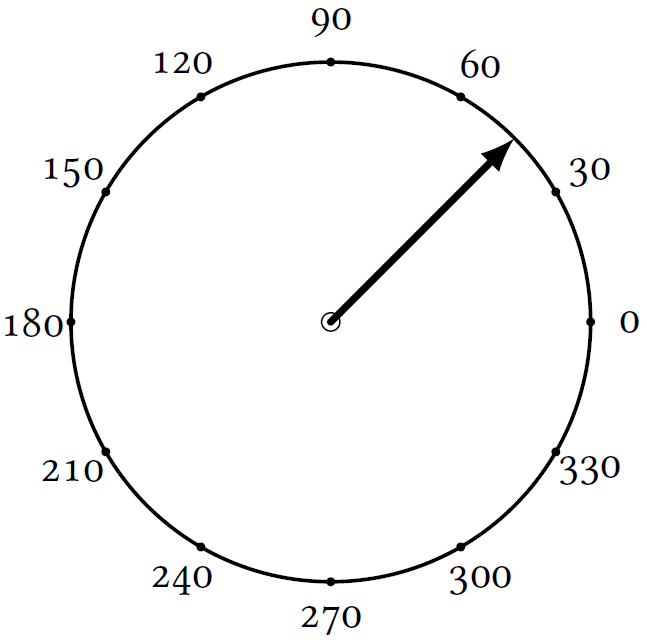
\includegraphics[width = .33\textwidth]{figs/kreis}
\caption{A fortune wheel.}
\label{fig:wheel}
\end{center}
\end{figure}

\subsection{Independence}
\mypar[Independence (1)]{Definition}\label{def:indep1}
  We say that two events $A, B$ are \term{independent} if
\[
  \Prob(A \cap B) = \Prob(A)\Prob(B).
\]
  Less formally, we can also say that $A, B$ are 
  independent \emph{of each other} or 
  that $A$ is independent of $B$ and vice versa.
\parend

\mypar{*Example}
  The event $\emptyset$ is independent of all other events.
  To see this, let $B$ be an arbitrary event.
  Since $\emptyset \cap B = \emptyset$, it follows that
  \[
    \Prob(\emptyset \cap B) 
    = \Prob(\emptyset) 
    = 0 
    = 0\cdot \Prob(B) 
    = \Prob(\emptyset)\Prob(B).
  \]
  The event $\Omega$ is also independent of all other events:
  Since for any event $B$, we have $\Omega \cap B = B$,
  it follows that
  \[
    \Prob(\Omega \cap B) 
    = \Prob(B) 
    = 1\cdot \Prob(B) 
    = \Prob(\Omega)\Prob(B).\parendeq
  \]

\mypar{Example}
  The events $A$ (\textit{The card shows an even number.})
  and $B$ (\textit{The card is of a black suit}) from the first random experiment
  are independent
  since
  \[
    \Prob(A \cap B) 
    = \frac{6}{36} 
    = \frac{12}{36} \cdot \frac{18}{36} 
    = \Prob(A)\Prob(B).
  \]
  The events $A \cup B$ and $A \cap B$, by contrast, are not independent
  since
  \[
    \Prob((A \cup B) \cap (A \cap B))
    = \Prob(A \cap B)
    = \frac{1}{6} 
    \neq \frac{2}{3} \cdot \frac{1}{6}
    = \Prob(A \cup B)\Prob(A \cap B).\parendeq
  \]

\mypar{Exercise}
  Consider the second random experiment.
  Are the events \textit{The first card is an Ace}
  and \textit{The second card is an Ace} independent?
  Justify your answer based on Definition \ref{def:indep1}.
\parend

\mypar{Exercise}
  Let $F, G$ be some events with $\Prob(F) = 0.6, \Prob(G) = 0.2$
  and $\Prob(F \cup G) = 0.72$.
  Are $F, G$ independent?
  Justify your answer based on Definition \ref{def:indep1}.
\parend

\mypar[Independence (2)]{Definition}\label{def:indep2} 
  We say that $n$ events $A_1, \dots, A_n$
  are \term{pairwise independent} if 
  $A_i, A_j$ are independent for all $1 \leq i < j \leq n$.
  
  We say that $n$ events $A_1, \dots, A_n$ are
  \term{independent} if, for each subset $I \subset \{1, \dots, n\}$, we have
  \[
    \Prob\left(\cap_{i \in I} A_i\right) = \prod_{i \in I}\Prob(A_i).
  \]
  In words: For \emph{every} choice of at most $n$ events from among the list,
  the probability that all chosen events occur simultaneously equals
  the product of the probabilities with which they occur individually.
  Independence implies pairwise independence.
  To see this, consider all subsets $I$ with two different events.
\parend

\mypar{*Example}
  We define the probability space consisting of the sample space
  \[
    \Omega := \{(0, 0, 0), (0, 1, 1), (1, 0, 1), (1, 1, 0)\}
  \]
  and a discrete uniform distribution, i.e.,
  $\Prob(\{\omega\}) = 1/4$ for all $\omega \in \Omega$. 
  We consider the events
  $A :=$ \textit{The first number is 1},
  $B :=$ \textit{The second number is 1},
  and $C :=$ \textit{The third number is 1}.
  As you can verify, $A, B, C$ are pairwise independent.
  Nonetheless,
\[
  \Prob(A \cap B \cap C) = 0 \neq \frac{1}{2} \cdot \frac{1}{2} \cdot \frac{1}{2} = \Prob(A)\Prob(B)\Prob(C).
\]
  Hence, $A,B,C$ are not independent.
\parend

We only need the next definition so that we can make sense of the
hypotheses for the Central Limit Theorem, which we'll encounter at the
end of this chapter.

\mypar[Independence (3)]{Definition} 
  A infinite family of events is \term{independent} if 
  each of its finite subfamilies is independent as per Definition \ref{def:indep2}.
\parend

\subsection{Conditional probabilities}
\mypar[Conditional probability]{Definition}\label{def:condprob}
  Let $A, B$ be events such that $\Prob(B) > 0$.
  We call
  \[
    \Prob(A | B) := \frac{\Prob(A \cap B)}{\Prob(B)}
  \]
  the \term{conditional probability of $A$ given $B$}.
  The conditional probability of $A$ given $B$ expresses
  the probability that $A$ occurs if you already know that $B$ has occurred.
\parend

\mypar{Remark} 
  If $A, B$ are independent with $\Prob(B) > 0$, then
  \begin{align*}
    \Prob(A | B)
    &= \frac{\Prob(A \cap B)}{\Prob(B)}   & [\textrm{Definition \ref{def:condprob}}] \\
    &= \frac{\Prob(A)\Prob(B)}{\Prob(B)}  & [\textrm{Definition \ref{def:indep1}}] \\
    &= \Prob(A).                          &
  \end{align*}
  This meshes with the intuition that if $A, B$ are independent, then
  knowing whether $B$ has occurred or not doesn't tell you anything new
  about whether $A$ will occur.
\parend

\mypar{Example}
  In the fortune wheel example, we may wonder about the probability that
  the arrow lands somewhere between 90 and 270 (`$A$') assuming that it
  landed between 0 and 120 (`$B$').
  We have $\Prob(B) = (120 - 0)/360 = 1/3$ and $\Prob(A \cap B) = (120 - 90)/(360) = 1/12$.
  Hence
  \[
    \Prob(A | B) = \frac{\Prob(A \cap B)}{\Prob(B)} = \frac{1/12}{1/3} = \frac{1}{4}.
  \]
  Since $\Prob(A) = (270-90)/360 = 1/2$, $\Prob(A | B) \neq \Prob(A)$.
  So $A,B$ are not independent.
\parend

The following theorem is useful for partioning a complex event into
simpler events.

\mypar[Total probability]{Theorem}\label{th:totprob}
Let $E_1, E_2, \dots$ be pairwise disjunct events that together comprise $\Omega$, i.e.,
$E_1 \cup E_2 \cup \dots = \Omega$.
Assume that $\Prob(E_k) > 0$ for all $k = 1, 2, \dots$.
Then, for each event $A$,
\[
  \Prob(A) = \sum_{k=1}^{\infty} \Prob(A | E_k) \Prob(E_k). \parendeq
\]
\begin{proof}
  We have
\begin{align*}
  \Prob(A)
  &= \Prob(A \cap \Omega)  \\
  &= \Prob(A \cap \bigcup_{k=1}^\infty E_k) \\
  &= \Prob\left(\bigcup_{k=1}^{\infty} (A \cap E_k)\right) \\
  &= \sum_{k=1}^{\infty} \Prob(A \cap E_k) \\
  &= \sum_{k=1}^{\infty} \Prob(A | E_k)\Prob(E_k).\qedhere
\end{align*}
\end{proof}

The above theorem, with the same proof, is also true if the list of pairwise
disjunct events is finite.


\mypar{*Example}
  Let's consider once more the second random experiment.
  The discrete uniform distribution on $\Omega_2$ assigns probability $1/1260$
  to each elementary event $\{(\omega_1, \omega_2)\}, (\omega_1, \omega_2) \in \Omega_2$.
  The probability that the first card drawn is the $6\clubsuit$ and the second is not a 6 is
  \[
    \frac{1}{36} \cdot \frac{36-4}{35} \approx 0.0254.
  \]
  Consequently, the probability that the first card is a 6 and the second one isn't is
  \[
    4\left(\frac{1}{36} \cdot \frac{36-4}{35}\right) \approx 0.1016.
  \]
  Similarly, we may compute the probability that the first card is some 7 and
  that the second's rank is greater than 7:
  \[
    4\left(\frac{1}{36} \cdot \frac{36-8}{35}\right) \approx 0.0889.
  \]
  The events \textit{The first card is a 6}, \textit{The first card is a 7}, \dots,
  are pairwise disjunct and together comprise the entire sample space.
  Hence, we may use the total probability theorem to compute the probability
  that the first card's rank is lower than the second card's rank:
  \begin{align*}
    \sum_{k = 1}^{9} 4\left(\frac{1}{36} \cdot \frac{36-4k}{35}\right)
    = \frac{4}{36\cdot 35} \sum_{k=1}^9 \left(36 - 4k\right)
    = \frac{4}{36\cdot 35}(9\cdot 36 - (4+8+\dots+36)).
  \end{align*}
  We can calculate the result in R:
\begin{knitrout}
\definecolor{shadecolor}{rgb}{0.969, 0.969, 0.969}\color{fgcolor}\begin{kframe}
\begin{alltt}
\hlnum{4}\hlopt{/}\hldef{(}\hlnum{36}\hlopt{*}\hlnum{35}\hldef{)} \hlopt{*} \hldef{(}\hlnum{9}\hlopt{*}\hlnum{36} \hlopt{-} \hlkwd{sum}\hldef{(}\hlnum{4}\hlopt{*}\hlkwd{seq}\hldef{(}\hlnum{1}\hldef{,} \hlnum{9}\hldef{)))}
\end{alltt}
\begin{verbatim}
[1] 0.4571429
\end{verbatim}
\end{kframe}
\end{knitrout}
That is, about 46\%.

  There's a more elegant way to arrive at the same solution.
  The probability that both cards have the same rank is $3/35$.
  So the probability that the card differ in rank is $32/35$.
  It is then clear that the probability that the first card is of
  lower rank than the second equals the probability that the first card is
  of greater rank that the second.
  Hence, the probability that the first card is of lower rank than the second
  rank is
  $(32/35)/2 \approx 0.4571$.
\parend

\mypar[M\&Ms]{Exercise}\label{ex:mm}
  M{\&}Ms come in six different colours;
  Table \vref{tab:mandms} lists their relative frequencies.
  When answering the following questions, 
  assume that the M{\&}Ms are drawn independently from an infinite population of M{\&}Ms.
\begin{enumerate}
  \item What's the probability that a randomly drawn M{\&}M is red or orange?
  \item What's the probability that, when you randomly draw two M{\&}Ms, both are red or orange?
  (That is, that both are red, both are orange, or one of them is red and the other is orange.)
  \item What's the probability that, when you randomly draw two M{\&M}s, one is red and the other orange?
  \item What's the probability that, when you randomly draw 5 M{\&}Ms, all of them are blue?
  \item What's the probability that, when you randomly draw 5 M{\&}Ms, none of them is blue?\parend
\end{enumerate}

\begin{table}
\centering
\caption{Relative frequencies of occurrence of M\&Ms by colour.}
\label{tab:mandms}
\begin{tabular}{@{}lr@{}}
\toprule
Colour  & Relative frequency \\ \midrule
Blue    & 23\%              \\
Orange  & 23\%              \\
Yellow  & 15\% \\
Green   & 15\% \\
Brown   & 12\% \\
Red     & 12\% \\
\bottomrule
\end{tabular}
\end{table}

Both in scientific and in societal discussions, the conditional probabilities
$\Prob(A | B)$ and $\Prob(B | A)$ are, unfortunately, often conflated.
The classic example below and the theorem following it tell you how 
$\Prob(A | B)$ and $\Prob(B | A)$ can be converted into one another.

\mypar[Medical screening]{Example}\label{example:medtest}
  Imagine that all newly born infants are subjected to a medical test
  that screens for a rare genetic disease.
  This genetic disease is thought to affect about 0.01\% of newborns.
  The test labels newborns affected with the disease as affected with probability 97\%.
  However, 1\% of newborns that are not affected by the disease will also be labelled as affected with the disease.
  If the test labels a newborn as affected by the disease, what's the probability that the newborn actually
  is affected by the disease?
  
  To answer this question, we can consider a large number of newborns, for instance, one million of them.
  Of these, about $0.0001 \cdot 10^6 = 100$ are expected to be affected by the disease;
  the remaining 999,900 aren't affected.
  Of these 100 affected children, 97 are expected to also be labelled as affected;
  the disease won't be flagged immediately in the remaining three ones.
  Of the 999,900 non-affected children, 
  $0.01 \cdot 999900 = 9999$ are expected to be falsely labelled as affected.
  If we randomly pick a child from the $97 + 9999 = 10096$ children that are expected to be labelled as affected,
  the probability that this child does indeed carry the disease is only $97/10096 \approx 0.0096$,
  that is, not even 1\%.
\parend

The procedure from the previous example can be applied generally,
as the famous Bayes' theorem shows.

\mypar[Bayes]{Theorem}
Let $A, B$ be events with $\Prob(A), \Prob(B) > 0$. 
Then 
\[
  \Prob(B | A)
  = \frac{\Prob(A|B)\Prob(B)}{\Prob(A|B)\Prob(B) + \Prob(A|B^c)(1 - \Prob(B))}. \parendeq
\]
\begin{proof}
We have
\begin{align*}
  \Prob(B | A)
  &= \frac{\Prob(B \cap A)}{\Prob(A)}     & [\textrm{Definition \ref{def:condprob}}] \\
  &= \frac{\Prob(A|B)\Prob(B)}{\Prob(A)}  & [\Prob(A|B)=\Prob(A \cap B)/\Prob(B)] \\
  &= \frac{\Prob(A|B)\Prob(B)}{\Prob(A|B)\Prob(B) + \Prob(A|B^c)(1 - \Prob(B))}. & [\textrm{total probability}]
\end{align*}
\end{proof}

In terms of Example \ref{example:medtest}, $B$ would be \textit{The child is affected}
and $A$ \textit{The child is labelled as affected}.
Then
$\Prob(A|B) = 0.97, \Prob(B) = 0.0001, \Prob(A | B^c) = 0.01$.
So, by Bayes' theorem,
\[
  \Prob(B | A) = \frac{0.97 \cdot 0.0001}{0.97 \cdot 0.0001 + 0.01 \cdot (1 - 0.0001)} \approx 0.0096.
\]

\section{Random variables}
When analysing quantitative data, we often model these
as observations of random variables.

\mypar[Random variables]{Definition}
  Let $\Omega$ be the sample space of a probability space.
  A \term{random variable} $X$ maps each outcome $\omega \in \Omega$ to a real number.
  
  If the set of possible values of $X$ is countable, we call $X$
  a \term{discrete random variable}.
\parend

\mypar{Example}\label{example:obenabe}
  In \textit{Jass}, we can consider the random variable $X$
  that maps each card to its point value in the \textit{Obenabe} mode of play,
  that is,
\begin{align*}
X(\omega) :=
\begin{cases}
  11, & \textrm{if $\omega$ is an Ace,} \\
  4,  & \textrm{if $\omega$ is a King,} \\
  3,  & \textrm{if $\omega$ is a Queen,} \\
  2,  & \textrm{if $\omega$ is a Jack,} \\
  10, & \textrm{if $\omega$ is a 10,} \\
  8,  & \textrm{if $\omega$ is an 8,} \\
  0,  & \textrm{else}.
\end{cases}
\end{align*}
This random variable is one of arbitrarily many you can define on $\Omega_1$.

If we draw two cards, you could define a random variable that represents, for instance,
the sum of the point values of both cards.
\parend

We can also consider the values that a random variable can take on as outcomes on their own.
This way, we obtain a new sample space
\[
  \widetilde{\Omega} := \{X(\omega) : \omega \in \Omega\}.
\]
For the random variable $X$, we'd have
\[
  \widetilde{\Omega}_1 = \{0, 2, 3, 4, 8, 10, 11\}.
\]
The probability that $X = 11$ is $4/36 = 1/9$. We write $\Prob(X = 11) = 1/9$.
Similarly, $\Prob(X = 0) = 1/3$.
We can also discuss events, for instance $\Prob(X \geq 10) = 2/9$.

Let's take a closer look at the most important representations and properties of
random variables.

\subsection{The distribution function and the quantile function}\label{sec:distributionfunction}
Random variables can be characterised by their \term{distribution function}.

\mypar[Distribution function]{Definition}
  Let $X$ be a random variable.
  The distribution function $F_X$ of $X$ is defined by
  \[
    F_X(r) := \Prob(X \leq r)
  \]
  for all real numbers $r$.
\parend

By way of example, consider random variable defined in Example \ref{example:obenabe}.
We can construct the following table with cumulative probabilities:

\begin{center}
\begin{tabular}{l|lllllll}
\hline
Value                       & 0     & 2     & 3     & 4     & 8     & 10    & 11  \\
Probability                 & 0.333 & 0.111 & 0.111 & 0.111 & 0.111 & 0.111 & 0.111 \\
Cumulative probability      & 0.333 & 0.444 & 0.555 & 0.666 & 0.777 & 0.888 & 1 \\
\hline
\end{tabular}
\end{center}

Thus, for instance, $F_X(-1) = 0, F_X(2.5) = 0.444$ and $F_X(12) = 1$.
Figure \ref{fig:fx} shows the distribution function of $X$.

\begin{knitrout}
\definecolor{shadecolor}{rgb}{0.969, 0.969, 0.969}\color{fgcolor}\begin{figure}[tp]

{\centering \includegraphics[width=.4\textwidth]{generated_figs/unnamed-chunk-216-1} 

}

\caption{Distribution function of the point value of \textit{Jass} cards in the \textit{Obenabe} mode of play.\label{fig:fx}}\label{fig:unnamed-chunk-216}
\end{figure}

\end{knitrout}

If we know the distribution function of a random variable,
we can compute the probability that the random variable lies in some interval:
\begin{align*}
  \Prob(X \in (-\infty, b]) = \Prob(X \leq b) = F_X(b), \\
  \Prob(X \notin (-\infty, a]) = \Prob(X > a) = 1 - F_X(a).
\end{align*}
So
\[
  \Prob(X \in (a, b]) = F_X(b) - F_X(a).
\]
We need to be somewhat more cautious when making probability claims
about intervals of the form $[a, b], [a, b)$ and $(a,b)$.
The reason is that the end points of such intervals may have some positive probability.
We therefore define a further function:
\[
  F_X(r-) := \Prob(X \in (-\infty, r)) = F_X(r) - \Prob(X = r).
\]
Consequently,
\begin{align*}
  \Prob(X \in [a, b]) &= F_X(b) - F_X(a-) = F_X(b) - F_X(a) + \Prob(X = a), \\
  \Prob(X \in [a, b)) &= F_X(b-) - F_X(a-) = F_X(b) - F_X(a) - \Prob(X = b) + \Prob(X = a), \\
  \Prob(X \in (a, b)) &= F_X(b-) - F_X(a) = F_X(b) - F(X)(a) - \Prob(X = b).
\end{align*}

Whereas the distribution function $F_X$ tells us the probability that a random
value assumes a value no larger than some number $r$, 
the \term{quantile function} $F^{-1}_X$ tells us the inverse:
Given some number $p \in (0,1)$, what is the lowest value $q$ such that
$F_X(q) \geq p$?

\mypar[Quantile function]{Definition}
  Let $X$ be a random variable.
  Its quantile function $F_X^{-1}$ is defined as
  \[
    F^{-1}_X(p) := \min\{q \in \mathbb{R} : F_X(q) \geq p\}. \parendeq
  \]

From Figure \ref{fig:fx}, we may, for instance, glean that
$F_X^{-1}(0.4) = 2$ and $F_X^{-1}(7/9) = 8$.

\mypar[Continuous uniform distribution]{Example}
  Consider the fortune wheel from Example \ref{example:wheel}.
  We define the random variable $X$ that quite simply tells us the 
  value the arrow points to.
  The distribution function of this random variable, shown in Figure \ref{fig:contuniform},
  is \term{continuous} (without jumps).
  The 0.3 quantile of this variable's distribution is $F^{-1}_{X}(0.3) = 108$.
\parend

\begin{knitrout}
\definecolor{shadecolor}{rgb}{0.969, 0.969, 0.969}\color{fgcolor}\begin{figure}[tp]

{\centering \includegraphics[width=.4\textwidth]{generated_figs/unnamed-chunk-217-1} 

}

\caption{Distribution function of a random variable with a continuous uniform distribution on $[0, 360)$.\label{fig:contuniform}}\label{fig:unnamed-chunk-217}
\end{figure}

\end{knitrout}

\subsection{Probability density functions}\label{sec:density}
The distribution of some random variables $X$ can be represented
by means of a \term{probability density function} $f_X$.
Let us get the formal definition out of the way before discussing what the
underlying idea is.

\mypar[Probability density function]{Definition}
  Let $X$ be a random variable and $F_X$ its distribution function.
  If there exists a non-negative function $f_X$ such that
  \[
    F_X(b) - F_X(a) = \int_a^b f_X(t) \df t
  \]
  for all real numbers $a, b$,
  then $f_X$ is a probability density function of $X$.
\parend

Figure \ref{fig:wheeldensity} shows what the idea is.
We want to represent the distribution of $X$ in such a way
that the probability that $X$ falls in a certain interval
corresponds to the area underneath the probability density function
over this interval.

\begin{knitrout}
\definecolor{shadecolor}{rgb}{0.969, 0.969, 0.969}\color{fgcolor}\begin{figure}[tp]

{\centering \includegraphics[width=0.4\textwidth]{generated_figs/unnamed-chunk-218-1} 

}

\caption{Probability density function of a variable following a continuous uniform distribution from 0 to 360. The probability of observing a value between 45 and 93 corresponds to the area underneath the density over this interval.\label{fig:wheeldensity}}\label{fig:unnamed-chunk-218}
\end{figure}

\end{knitrout}

For a random variable $X$ with a continuous uniform distribution on $[0, 360)$,
one possible probability density function is
\[
  f_X(x) =
  \begin{cases}
    \frac{1}{360}, & \textrm{if $x \in [0, 360)$}, \\
    0, & \textrm{else.}
  \end{cases}
\]
As you may recall from school, the area underneath a curve over an interval is given
by the integral of the function over this interval.
Indeed, we have
\[
  \Prob(X \in [45, 93]) 
  = \int_{45}^{93} f_X(t) \df t 
  = \int_{45}^{93} \frac{1}{360} \df t 
  = \frac{t}{360} \Big|_{45}^{93}
  = \frac{93 - 45}{360}.
\]

\mypar{Remark}
  Not all random variables have a probability density function.
  If a random variable has a probability density function,
  then its distribution function is continuous.
  That said, it is possible for a random variable to have a continuous
  distribution function but no probability density function.
  Such random variables are difficult to construct, though.
\parend

\mypar{*Remark}  
  If a random variable has \emph{a} probability
  density function, then it has an infinite number of them:
  Given a suitable probability density function $f_X$, we may define
  another one by changing the value of $f_X$ at one single arbitrary point.
  This doesn't affect the integral.
  That said, if the distribution function $F_X$ is not only continuous
  but also differentiable,
  then the derivative of $F_X$ is a probability density function of $X$
  and is considered the canonical one.
\parend

\mypar{Definition}
  If a random variable has a probability density function,
  we call it \term{(absolutely) continuous}.
\parend

We'll have a look at some examples of continuous probability distributions
in Section \ref{sec:continuousdists}.

\mypar{*Remark}
  An absolutely continuous random variable cannot be discrete and vice versa:
  If $X$ has a probability density function $f_X$, then
  \[
    \Prob(X = r) = \int_r^r f_X(t) \df t = 0
  \]
  for all real numbers $r$. 
  If $X$ is discrete, however, there must be some $r$ such that $\Prob(X = r) > 0$.
  
  However, random variables can be neither absolutely continuous nor discrete.
  One example would the amount of precipitation on a given day in a given area.
  It's possible that there's a 70\% chance of no precipitation ($\Prob(X = 0) = 0.7$),
  but that, if there is some precipitation, then the amount of precipitation is
  absolutely continuous.
\parend

\subsection{The expected value and the variance}
Before we have a closer look at some classic probability distributions,
let's introduce the two most commonly used numeric properties of random variables
(or of their probability distributions).
The first property is the \term{expected value} (also called \term{expectation}
or \term{mean}), which expresses which value the random variable takes on on average.
The expected value generalises the arithmetic mean, which can straightforwardly
be computed if you have a finite number of values, to sample spaces of arbitrary size.

If $X$ is a discrete random variable on a sample space $\Omega$,
then its expected value $\E(X)$ can be computed as
\[
  \E(X) = \sum_{x \in \Omega} x\Prob(X = x),
\]
if this sum is a well-defined real number.\footnote{It is possible for the sum to depend
on the order in which we enumerate $\Omega$, in which case it isn't well-defined.
It's also possible for this sum to diverge to $-\infty$ or $\infty$,
in which case it isn't a real number. We won't deal with such pathological distributions, though.}
In the \textit{Obenabe} example (Example \ref{example:obenabe}), we hence have
\begin{align*}
  \E(X) = 0\cdot \frac{1}{3} + 2 \cdot \frac{1}{9} + 3 \cdot \frac{1}{9}
          + 4 \cdot \frac{1}{9} + 8 \cdot \frac{1}{9} + 10 \cdot \frac{1}{9}
          + 11 \cdot \frac{1}{9}
        = 4.22.
\end{align*}
As a further example consider the random variable $G$ generated by the random number
generator from Example \ref{example:2k}.
Its expectation is\label{expectation_2k}
\[
  \E(G) = \sum_{k=1}^{\infty} k\Prob(G = k) = \sum_{k=1}^{\infty}\frac{k}{2^k} = 2.
\]
For this course, you don't have to be able to compute expected values for 
distributions with infinite sample spaces. 
The idea here is merely to show that the arithmetic mean can be generalised
to cases with an infinite number of values.

Incidentally, and more generally, it holds that
\[
  \E(g(X)) = \sum_{x \in X(\Omega)} g(x)\Prob(X = x)
\]
for each function $g$, if this sum is a well-defined real number.

If the random variable $X$ has a probability density function $f_X$,
then its expectation can be computed as
\[
  \E(X) = \int_{-\infty}^{\infty} xf_X(x) \df x,
\]
if this integral is a well-defined real number.
In the fortune wheel example, for instance,
\begin{align*}
  \E(W)
  &= \int_{-\infty}^{\infty} x f_X(x) \df x \\
  &= \int_{0}^{360} \frac{x}{360} \df x \\
  &= \frac{1}{360} \left.\left[\frac{1}{2}x^2\right]\right|_0^{360} \\
  &= \frac{360^2}{2\cdot 360} \\
  &= 180.
\end{align*}

More generally,
\[
  \E(g(X)) = \int_{-\infty}^{\infty} g(x)f_X(x) \df x,
\]
for (essentially) each function $g$, if this integral is a well-defined real number.\footnote{Regarding `essentially': It is possible
to construct so-called non-measurable functions $g$ that cannot be integrated.}

If a probability distribution is neither absolutely continuous nor discrete,
one can compute the expectations of its continuous and its discrete parts separately
and then combine them using a suitable weighting.
We'll only discuss discrete and absolutely continuous distributions, though.

\mypar[Properties of the expected value]{Lemma}
  Let $X, Y$ be random variables.
  If $X$ is constant, that is, $X \equiv c$, then $\E(X) = c$.
  
  The expected value is \term{linear}.
  This means that $\E(aX + bY) = a\E(X) + b\E(Y)$ for constants $a, b$, 
  if $\E(X)$ and $\E(Y)$ exist in the first place.
  This property follows from the linearity of finite and infinite sums
  as well as from the linearity of integrals.
\parend

The expected value expresses which value the random variable takes on on average.
But it would be useful to also have some numerical measure that expresses
how large the discrepancies between individual instantiations of this random
variable and its expected value are expected to be.
At first blush, it would seem to make sense to compute the expected value
of these discrepancies, that is,
\[
  \E(X - \E(X)).
\]
By linearity of the expected value, however,
\[
  \E(X - \E(X)) = \E(X) - \E(\E(X)) = \E(X) - \E(X) = 0
\]
for each random variable $X$ that has an expected value.
So this measure doesn't carry any information.
A more useful measure is the expected value of the absolute discrepancies, that is,
\[
  \E(|X - \E(X)|).
\]
While this measure is sometimes used, it's cumbersome to use.
Instead, one usually works with the expected value of the squared discrepancies,
that is,
\[
  \E((X - \E(X))^2).
\]
If $X$ is a random variable such that this measure exists,
we call $\Var(X) := \E((X - \E(X))^2)$ the \term{variance} of $X$.\footnote{Not all random variables have
a variance. This includes all random variable that do not have an expected value.}

\mypar{Lemma}\label{lemma:steiner}
  If $X$ is a random variable such that $\Var(X)$ exists, then
  \[
    \Var(X) = \E(X^2) - \E(X)^2. \parendeq
  \]
\begin{proof}
  We expand the expression in the definition and then apply properties of the expected value:
\begin{align*}
  \Var(X)
  &= \E((X - \E(X))^2)                  & [\textrm{Definition}]\\
  &= \E(X^2 - 2X\E(X) + \E(X)^2)        & [\textrm{$(a-b)^2 = a^2 - 2ab + b^2$}] \\
  &= \E(X^2) - 2\E(X(\E(X))) + \E(X)^2  & [\textrm{Linearity of $\E$}] \\
  &= \E(X^2) - 2\E(X)^2 + \E(X)^2       & [\textrm{$\E(X)$ is constant}]\\
  &= \E(X^2) - \E(X)^2.                 & 
\end{align*}
\end{proof}

If a random variable is expressed in some unit (e.g., seconds),
then its variance is expressed in the square of this unit (e.g., squared seconds).
By taking the root of the variance, we get rid of these squared units.
The numerical property so obtained is called the random variable's \term{standard deviation}:
$\sqrt{\Var(X)} =: \Std(X)$.

\mypar{Example}
  Lemma \ref{lemma:steiner} allows us to compute variances quite straightforwardly.
  In the \textit{Obenabe} example, we have
\begin{align*}
  \E(X^2) = 0^2\cdot \frac{1}{3} + 2^2 \cdot \frac{1}{9} + 3^2 \cdot \frac{1}{9}
          + 4^2 \cdot \frac{1}{9} + 8^2 \cdot \frac{1}{9} + 10^2 \cdot \frac{1}{9}
          + 11^2 \cdot \frac{1}{9}
        = 34.89.
\end{align*}
  Hence, the variance of the random variable in the \textit{Obenabe} example is
  \[
    \E(X^2) - \E(X)^2 = 34.89 - 4.22^2 = 17.08.
  \]
  So its standard deviation is $\sqrt{17.08} \approx 4.13$.

  For the random number generator in Example \ref{example:2k}, we have
  \[
    \E(G^2) = \sum_{k=1}^{\infty} \frac{k^2}{2^k} = 6.
  \]
  (This computation is not obvious; for the purposes of this course,
  we may consider the result as given.)
  Hence, the variance of $G$ is
  \[
    \Var(G) = \E(G^2) - \E(G)^2 = 6 - 2^2 = 2.
  \]
  So its standard deviation is $\sqrt{2}$.

  In the fortune wheel example, we have
  \[
    \E(W^2) = \int_{0}^{360}\frac{t^2}{360} \df t = \frac{360^3}{3\cdot 360} = 43200.
  \]
  So the variance of $W$ is
  \[
    \E(W^2) - \E(W)^2 = 43200 - 180^2 = 10800.
  \]
  So its standard deviation is $\sqrt{10800} \approx 103.9$.
\parend

\mypar[Properties of the variance]{Lemma}\label{properties_variance}
  Let $X$ be a random variable such that $\Var(X)$ exists
  and let $a, b$ be constants.
  Then
  \[
    \Var(aX + b) = a^2\Var(X). \parendeq
  \]
\begin{proof}
  We have
  \begin{align*}
    \Var(aX + b)
    &= \E\left(\left(aX + b - \E\left(aX + b\right)\right)^2\right) \\
    &= \E\left(\left(aX + b - a\E\left(X\right) - b\right)^2\right) \\
    &= \E\left(a^2\left(X - \E(X)\right)^2\right) \\
    &= a^2\E\left(\left(X - \E(X)\right)^2\right) \\
    &= a^2\Var(X). \qedhere
  \end{align*}
\end{proof}
  
  In general, though, it is \emph{not} the case that 
  $\Var(X + Y) = \Var(X) + \Var(Y)$.
  If $X, Y$ are independent 
  (with independence of random variables being defined in the next section),
  however, it \emph{is} true that $\Var(X + Y) = \Var(X) + \Var(Y)$.

\mypar{Example}
  Based on the random variable $G$ from Example \ref{example:2k},
  we define the random variable $\widetilde{G} := 3G + 4$.
  By the properties of the expected value and the variance, we obtain
  \[
    \E(\widetilde{G}) = \E(3G + 4) = 3\E(G) + 4 = 10
  \]
  and
  \[
    \Var(\widetilde{G}) = \Var(3G + 4) = 3^2\Var(G) = 18.\parendeq
  \]

\mypar[Variance of a sum $\neq$ sum of the variances]{Example}
  Based on the random variable $G$ from Example \ref{example:2k},
  we define the random variable $\overline{G} := -G$.
  Then $G + \overline{G} = G - G = 0$.
  So
  \[
    \Var(G + \overline{G}) = 0 \neq 4 = \Var(G) + \Var(\overline{G}).
  \]
  It's intuitively clear that $G, \overline G$ are not independent.
  This intuition is formalised in the next section.
\parend

\subsection{Independence}
\mypar[Independence of random variables]{Definition}\label{def:indep_rv}
  Let $X, Y$ be random variables.
  We say that $X, Y$ are \term{independent} if, for any set of numbers $E_1, E_2$
  about which it's possible to make probabilistic claims (cf.\ the comment on page \pageref{comment:measurable}),
  it is the case that
  \[
    \Prob(X \in E_1, Y \in E_2) = \Prob(X \in E_1)\Prob(Y \in E_2).
  \]
  This definition for the independence of two random variables
  can be generalised to the definition of multiple and of an infinite number
  of random variables in the same way that the definition of independence
  of two events was generalised.
\parend

Conceptually, independence of $X, Y$ means that knowing the value that
$X$ takes on doesn't provide any information as to the value of $Y$, and vice versa.
If random variables are independent, the sum of their variances can easily
be computed, as per the next lemma, which is presented without proof.

\mypar{Lemma}
  Let $X, Y$ be independent random variables with existing variance.
  Then
  \[
    \Var(X + Y) = \Var(X) + \Var(Y). \parendeq
  \]

\section{Examples of discrete probability distributions}

\subsection{The discrete uniform distribution}
Let $n$ be a natural number and 
$\Omega := \{1, \dots, n\}$.
Let $X$ be the random variable defined by $X(k) = k$ for each $k \in \Omega$.
If, for each $k \in \Omega$, $\Prob(X = k) = 1/n$, then $X$ has a
\term{discrete uniform distribution} on $\Omega$.
We write $X \sim \textrm{Unif}(\Omega)$.

The classic example for such a discrete uniform distribution is a throw
with a fair six-sided dice.
In this example, we have $\Prob(X = k) = 1/6$ for $k \in \{1, 2, 3, 4, 5, 6\}$
and $\Prob(X = k) = 0$ for all $k \notin \{1, \dots, 6\}$.

The expected value of a random variable $X$ with a discrete uniform distribution
over the sample space $\{1, 2, \dots, n\}$ is
\[
  \E(X) = \frac{1}{n}(1 + 2 + \dots + n) = \frac{n(1+n)}{2n} = \frac{1+n}{2},
\]
which should make sense intuitively.
Its variance is
\[
  \Var(X) = \frac{n^2 - 1}{12},
\]
which we won't derive ourselves.

More generally, let $X$ be a random variable with a discrete uniform distribution over
\[
  \Omega := \{a, a + 1, a + 2, \dots, b - 2, b - 1, b\}.
\]
Then
\[
  \E(X) = \frac{a + b}{2}, \Var(X) = \frac{(b - a + 1)^2 - 1}{12}.
\]

\mypar{*Exercise}
  Let $X$ be a random variable with a discrete uniform distribution over
  \[
    \{1, 2, \dots, n-2, n-1\}.
  \]
  Define $Y := X/2 + 1/2$.
  Then $Y$ has a discrete uniform distribution over
  \[
    \{1, 1.5, 2, \dots, n/2\}.
  \]
  Use the properties of the expected value and the variance to determine
  $\E(Y), \Var(Y)$.
\parend

\mypar[Generating data from a discrete uniform distribution]{Remark}
  In the upcoming sections and chapters, we'll try to get a handle on concepts by
  means of simulations.
  These will require us to generate data from certain distributions.
  The following snippet shows how we can generate \texttt{n\_obs} independent
  data points from a discrete uniform distribution on $\{1, \dots, n\}$.
\begin{knitrout}
\definecolor{shadecolor}{rgb}{0.969, 0.969, 0.969}\color{fgcolor}\begin{kframe}
\begin{alltt}
\hlcom{# Define sample space}
\hldef{n} \hlkwb{<-} \hlnum{6}
\hldef{Omega} \hlkwb{<-} \hlnum{1}\hlopt{:}\hldef{n}
\hlcom{# Generate n_obs observations discrete unif. dist. on sample space}
\hldef{n_obs} \hlkwb{<-} \hlnum{20}
\hldef{observations} \hlkwb{<-} \hlkwd{sample}\hldef{(Omega, n_obs,} \hlkwc{replace} \hldef{=} \hlnum{TRUE}\hldef{)}
\hldef{observations}
\end{alltt}
\begin{verbatim}
 [1] 4 2 2 1 3 2 2 1 3 3 1 6 4 4 2 5 3 3 1 3
\end{verbatim}
\end{kframe}
\end{knitrout}
\parend

\subsection{The Bernoulli distribution}\label{sec:bernoulli}
The \term{Bernoulli distribution} models the outcome $X$ of a random experiment
with two possible outcomes, which are labelled $0$ (`failure') and $1$ (`success').
It has a parameter $p \in [0,1]$, where $\Prob(X = 1) = p$ and $\Prob(X = 0) = 1-p$.
If a random variable $X$ follows a Bernoulli distribution with parameter $p$,
we write $X \sim \textrm{Bernoulli}(p)$.

The expected value of a $\textrm{Bernoulli}(p)$-distributed random variable $X$
is easily computed:
\[
  \E(X) = 0\cdot(1-p) + 1\cdot p = p.
\]
Similarly,
\[
  \E(X^2) = 0^2\cdot(1-p) + 1^2\cdot p = p.
\]
Hence,
\[
  \Var(X) = p - p^2 = p(1-p).
\]

\mypar{Example}
  We draw a random card from a deck of 36 \textit{Jass} cards.
  The probability that we've drawn an Ace is $p = 4/36 = 1/9$.
  We can thus model the random experiment `Drawing an Ace' as a Bernoulli
  experiment with parameter $p = 1/9$,
  where we label the outcome of the experiment as 1 if we draw an Ace
  and 0 otherwise.
\parend

\subsection{The binomial distribution}\label{sec:binomial}
Let $X_1, \dots, X_n$ be independent random variables that all
follow a $\textrm{Bernoulli}(p)$ distribution.
Then $X := X_1 + \dots + X_n$ is said to follow a \term{binomial distribution}
with parameters $n$ and $p$.
We write $X \sim \textrm{Binomial}(n, p)$.
In words, the binomial distribution models the number of $n$ independent and
identical Bernoulli experiments that have successful outcomes.

By the linearity of the expected value,
\[
  \E(X) = \E(X_1) + \dots + \E(X_n) = np.
\]
By the independence of $X_1, \dots, X_n$,
\[
  \Var(X) = \Var(X_1) + \dots + \Var(X_n) = np(1-p).
\]


The probability that precisely the first $k$ of $n$ independent and identical
Bernoulli experiments produce a success is
\[
  \Prob(X_1 = 1)\Prob(X_2 = 1) \cdots \Prob(X_k = 1)\Prob(X_{k+1} = 0)\cdots\Prob(X_n = 0) = p^k(1-p)^{n-k}.
\]
There are $n \cdot (n-1) \cdot \dots \cdot 1 = n!$ possibilities to reorder 
these Bernoulli experiments.
Since neither the outcomes of the first $k$ of these experiments
nor the outcomes of the last $n-k$ ones can be distinguished from one another,
there are
\[
  \frac{n!}{k!(n-k)!} =: \binom{n}{k}
\]
different possible orders in which these outcomes can be observed.
Hence, the probability that exactly $k$ of $n$ independent and identical
Bernoulli experiments produce a success is
\[
  \Prob(X = k) = \binom{n}{k}p^k(1-p)^{n-k}.
\]
The number $\binom{n}{k}$ is called the \term{binomial coefficient} of $n$ and $k$.
We also say `$n$ choose $k$'.
For $k < 0$ or $k > n$, we define $\binom{n}{k} = 0$.
Consequently, the distribution function of a Binomial($n$, $p$) distribution is
\[
  F(r) = \sum_{k = 0}^{\lfloor r \rfloor} \binom{n}{k}p^k(1-p)^{n-k}.
\]

The binomial coefficient $\binom{n}{k}$ can be calculated using the
R command \texttt{choose(n, k)}.
R also features some functions that can be used to retrieve information
about the binomial distribution and that can generate data from a binomial
distribution.
As an example, imagine that we throw a 6-sided dice ten times and count
how often we've thrown a 6.
This outcome can be modelled by means of a Binomial($10$, $1/6$) distribution.
The function \texttt{dbinom()} allows us compute $\Prob(X = k)$.
For instance, the probability that we throw exactly five sixes is about 1.3\%:
\begin{knitrout}
\definecolor{shadecolor}{rgb}{0.969, 0.969, 0.969}\color{fgcolor}\begin{kframe}
\begin{alltt}
\hlkwd{dbinom}\hldef{(}\hlnum{5}\hldef{,} \hlnum{10}\hldef{,} \hlnum{1}\hlopt{/}\hlnum{6}\hldef{)}
\end{alltt}
\begin{verbatim}
[1] 0.01302381
\end{verbatim}
\end{kframe}
\end{knitrout}
Figure \ref{fig:dbinom} shows $\Prob(X = k)$ for
$X \sim \textrm{Binomial}(10, 1/6)$ and $k = 0, \dots, 10$.

\begin{knitrout}
\definecolor{shadecolor}{rgb}{0.969, 0.969, 0.969}\color{fgcolor}\begin{figure}[tp]

{\centering \includegraphics[width=.8\textwidth]{generated_figs/unnamed-chunk-221-1} 

}

\caption{Left: Probability of the number of successes in a Binomial($10$, $1/6$) distribution. Right: Distribution function of the same distribution.\label{fig:dbinom}}\label{fig:unnamed-chunk-221}
\end{figure}

\end{knitrout}

The function \texttt{pbinom()} can be used to retrieve $\Prob(X \leq k)$.
For instance, the probability that we throw no more than two sixes is about 78\%:
\begin{knitrout}
\definecolor{shadecolor}{rgb}{0.969, 0.969, 0.969}\color{fgcolor}\begin{kframe}
\begin{alltt}
\hlkwd{pbinom}\hldef{(}\hlnum{2}\hldef{,} \hlnum{10}\hldef{,} \hlnum{1}\hlopt{/}\hlnum{6}\hldef{)}
\end{alltt}
\begin{verbatim}
[1] 0.7752268
\end{verbatim}
\end{kframe}
\end{knitrout}
The probability that we throw more than two sixes is hence about 22\%.
Similarly, the probability that we throw at least two sixes is about 52\%:
\begin{knitrout}
\definecolor{shadecolor}{rgb}{0.969, 0.969, 0.969}\color{fgcolor}\begin{kframe}
\begin{alltt}
\hlnum{1} \hlopt{-} \hlkwd{pbinom}\hldef{(}\hlnum{1}\hldef{,} \hlnum{10}\hldef{,} \hlnum{1}\hlopt{/}\hlnum{6}\hldef{)}
\end{alltt}
\begin{verbatim}
[1] 0.5154833
\end{verbatim}
\begin{alltt}
\hlkwd{pbinom}\hldef{(}\hlnum{1}\hldef{,} \hlnum{10}\hldef{,} \hlnum{1}\hlopt{/}\hlnum{6}\hldef{,} \hlkwc{lower.tail} \hldef{=} \hlnum{FALSE}\hldef{)}
\end{alltt}
\begin{verbatim}
[1] 0.5154833
\end{verbatim}
\end{kframe}
\end{knitrout}

The \texttt{qbinom()} function retrieves the quantiles of the Binomial($n$, $p$)
distribution:
\begin{knitrout}
\definecolor{shadecolor}{rgb}{0.969, 0.969, 0.969}\color{fgcolor}\begin{kframe}
\begin{alltt}
\hlkwd{qbinom}\hldef{(}\hlnum{0.70}\hldef{,} \hlnum{10}\hldef{,} \hlnum{1}\hlopt{/}\hlnum{6}\hldef{)}
\end{alltt}
\begin{verbatim}
[1] 2
\end{verbatim}
\begin{alltt}
\hlkwd{qbinom}\hldef{(}\hlnum{0.75}\hldef{,} \hlnum{10}\hldef{,} \hlnum{1}\hlopt{/}\hlnum{6}\hldef{)}
\end{alltt}
\begin{verbatim}
[1] 2
\end{verbatim}
\begin{alltt}
\hlkwd{qbinom}\hldef{(}\hlnum{0.80}\hldef{,} \hlnum{10}\hldef{,} \hlnum{1}\hlopt{/}\hlnum{6}\hldef{)}
\end{alltt}
\begin{verbatim}
[1] 3
\end{verbatim}
\end{kframe}
\end{knitrout}
In other words, if lots of people were to throw a dice ten times each,
at least 70\% of them would throw at most two sixes.
In fact, at least 75\% of them would throw at most two sixes.
At least 80\% of them would throw at most three sixes.
In fact, about 77.5\% of them would throw at most two sixes,
as we can compute using \texttt{pbinom()}:
\begin{knitrout}
\definecolor{shadecolor}{rgb}{0.969, 0.969, 0.969}\color{fgcolor}\begin{kframe}
\begin{alltt}
\hldef{k} \hlkwb{<-} \hlnum{0}\hlopt{:}\hlnum{10}
\hlkwd{tibble}\hldef{(}\hlkwc{k} \hldef{= k,}
       \hlsng{"Prob(X <= k)"} \hldef{=} \hlkwd{pbinom}\hldef{(k,} \hlnum{10}\hldef{,} \hlnum{1}\hlopt{/}\hlnum{6}\hldef{))}
\end{alltt}
\begin{verbatim}
# A tibble: 11 x 2
      k `Prob(X <= k)`
  <int>          <dbl>
1     0          0.162
2     1          0.485
3     2          0.775
4     3          0.930
5     4          0.985
6     5          0.998
7     6          1.000
# i 4 more rows
\end{verbatim}
\end{kframe}
\end{knitrout}

The function \texttt{rbinom()} can be used to generate independent
observations from a binomial distribution. Let's say that we wanted
to simulate the number of sixes produced by each of twenty people throwing
the dice 10 times:
\begin{knitrout}
\definecolor{shadecolor}{rgb}{0.969, 0.969, 0.969}\color{fgcolor}\begin{kframe}
\begin{alltt}
\hlkwd{rbinom}\hldef{(}\hlnum{20}\hldef{,} \hlnum{10}\hldef{,} \hlnum{1}\hlopt{/}\hlnum{6}\hldef{)}
\end{alltt}
\begin{verbatim}
 [1] 2 2 1 1 1 0 5 2 1 0 2 3 2 3 2 3 1 3 0 1
\end{verbatim}
\end{kframe}
\end{knitrout}

The Bernoulli($p$) distribution is the same as the Binomial($1$, $p$) distribution.

\section{Examples of continuous probability distributions}\label{sec:continuousdists}
\subsection{The continuous uniform distribution}
We've already encountered the continuous uniform distribution in the 
fortune wheel example.
More generally, we denote as $\textrm{Unif}([a,b])$ the continuous
uniform distribution on the interval $[a, b], a < b$.
The endpoints can be included or left out at will; 
the distribution doesn't change as a a result.
For $X \sim \textrm{Unif}([a,b])$, we have
\[
  \E(X) = \frac{a+b}{2}
\]
and
\[
  \Var(X) = \frac{(b-a)^2}{12}.
\]
A density function for a continuous uniform distribution on $[a,b]$ is
\[
  f_U(x) =
  \begin{cases}
    \frac{1}{b-a}, & \textrm{if $x \in [a, b]$}, \\
    0, &\textrm{otherwise}.
  \end{cases}
\]
The distribution function is
\[
  F_U(r) =
  \begin{cases}
    0, & \textrm{if $r < a$}, \\
    \frac{r - a}{b-a}, & \textrm{if $r \in [a,b]$}, \\
    1, & \textrm{if $r > b$}.
  \end{cases}
\]

We can evaluate a valid density function at a given point using 
\texttt{dunif()}. For instance, for a continuous uniform distribution on
$[-\pi, \pi]$, we find
\begin{knitrout}
\definecolor{shadecolor}{rgb}{0.969, 0.969, 0.969}\color{fgcolor}\begin{kframe}
\begin{alltt}
\hlkwd{dunif}\hldef{(}\hlnum{2}\hldef{,} \hlopt{-}\hldef{pi, pi)} \hlcom{# = 1/(2*pi)}
\end{alltt}
\begin{verbatim}
[1] 0.1591549
\end{verbatim}
\begin{alltt}
\hlkwd{dunif}\hldef{(}\hlnum{4}\hldef{,} \hlopt{-}\hldef{pi, pi)}
\end{alltt}
\begin{verbatim}
[1] 0
\end{verbatim}
\end{kframe}
\end{knitrout}
The distribution function is implemented in \texttt{punif()}:
\begin{knitrout}
\definecolor{shadecolor}{rgb}{0.969, 0.969, 0.969}\color{fgcolor}\begin{kframe}
\begin{alltt}
\hlkwd{punif}\hldef{(}\hlnum{2}\hldef{,} \hlopt{-}\hldef{pi, pi)}
\end{alltt}
\begin{verbatim}
[1] 0.8183099
\end{verbatim}
\end{kframe}
\end{knitrout}
That is, if $X \sim \textrm{Unif}([-\pi, \pi])$,
then $\Prob(X \leq 2) \approx 82\%$.
Using \texttt{qunif()}, we can obtain the quantiles of this distibution;
using \texttt{runif()}, we can generate independent observations from it:
\begin{knitrout}
\definecolor{shadecolor}{rgb}{0.969, 0.969, 0.969}\color{fgcolor}\begin{kframe}
\begin{alltt}
\hlkwd{runif}\hldef{(}\hlnum{10}\hldef{,} \hlopt{-}\hldef{pi, pi)}
\end{alltt}
\begin{verbatim}
 [1] -0.9495818 -0.8845674 -1.9287873 -2.7450394  0.1155496
 [6]  2.3338782  2.8062412 -1.0700206  2.5539018  0.3239638
\end{verbatim}
\end{kframe}
\end{knitrout}

\subsection{The normal distribution}
The \term{normal distribution} occupies a central space in the theory and practice
of probability theory, statistics, and data analysis.
The normal distribution has two parameters:
its expected value $\mu$, and its variance $\sigma^2$.
If a random variable $X$ follows 
a normal distribution with parameters $\mu, \sigma^2$,
we can write $X \sim \textrm{Normal}(\mu, \sigma^2)$ or $X \sim \mathcal{N}(\mu, \sigma^2)$.
Figure \ref{fig:dnorm} shows density functions for normal distributions with
four different parameter combinations.
The plot in the top left shows the \term{standard normal distribution},
that is, the normal distribution with mean 0 and variance 1.


\begin{knitrout}
\definecolor{shadecolor}{rgb}{0.969, 0.969, 0.969}\color{fgcolor}\begin{figure}[tp]

{\centering \includegraphics[width=.6\textwidth]{generated_figs/unnamed-chunk-230-1} 

}

\caption{Density functions of four normal distributions.\label{fig:dnorm}}\label{fig:unnamed-chunk-230}
\end{figure}

\end{knitrout}

The canonical density function $f$ of a  $\mathcal{N}(\mu, \sigma^2)$ distribution
is 
\[
  f(x) = \frac{1}{\sqrt{2\pi}\sigma}\exp\left\{\frac{-(x-\mu)^2}{2\sigma}\right\},
\]
where $\exp\{\cdot\}$ is the exponential function.
This formula isn't too important for us.
It suffices to appreciate that $\mu$ determines the central tendency of the
normal distribution, whereas $\sigma^2$ determines how tall and how wide it is.
The distribution function of a normal distribution cannot be represented analytically.

The R functions \texttt{dnorm()}, \texttt{pnorm()}, and \texttt{rnorm()}
can be used to evalute the density and distribution functions, and to 
generate independent observations from normal distributions.
Importantly, R parametrises normal distributions using their standard deviation
rather than using their variance.
For instance, consider $X \sim \mathcal{N}(3, 16)$. 
Then we can compute $\Prob(X \leq 0)$ as follows; also see Figure \ref{fig:dnormex}:
\begin{knitrout}
\definecolor{shadecolor}{rgb}{0.969, 0.969, 0.969}\color{fgcolor}\begin{kframe}
\begin{alltt}
\hlkwd{pnorm}\hldef{(}\hlnum{0}\hldef{,} \hlkwc{mean} \hldef{=} \hlnum{3}\hldef{,} \hlkwc{sd} \hldef{=} \hlkwd{sqrt}\hldef{(}\hlnum{16}\hldef{))}
\end{alltt}
\begin{verbatim}
[1] 0.2266274
\end{verbatim}
\end{kframe}
\end{knitrout}

\begin{knitrout}
\definecolor{shadecolor}{rgb}{0.969, 0.969, 0.969}\color{fgcolor}\begin{figure}[tp]

{\centering \includegraphics[width=.8\textwidth]{generated_figs/unnamed-chunk-232-1} 

}

\caption{The $\mathcal{N}(3, 16)$ distribution. Left: The probability of observing a value lower than 0 corresponds to the area under the curve up till 0. Right: We can compute this probability using the distribution function.\label{fig:dnormex}}\label{fig:unnamed-chunk-232}
\end{figure}

\end{knitrout}


\mypar[IQ]{Exercise} 
  The distribution of IQ scores in a population can be modelled
  as a $\mathcal{N}(100, 15^2)$ distribution.
  Use the \texttt{pnorm()} und \texttt{qnorm()} functions
  in order to answer the questions below.
  For the last three questions, you may want to also use
  the binomial distribution, but you don't have to.
\begin{enumerate}
\item What's the probability that a randomly picked person has an IQ lower than 90?
\item What's the probability that a randomly picked person has an IQ higher than 85?
\item What's the probability that a randomly picked person has an IQ between 110 and 120?
\item What's the probability that a randomly picked person has an IQ that lies
at least a standard deviation away from the mean?
\item For which IQ score is it the case that 25\% of the population has a lower IQ
score and 75\% of the population has a higher IQ score?
\item A person is `of average intelligence' if their IQ score belongs to the 
      middle 45\% of the population.
      Between which two IQ scores does average intelligence fall?
\item You randomly pick two people and obtain their IQ scores.
      What's the probability that none of them has an IQ higher than 105?
\item You randomly pick three people and obtain their IQ scores.
      What's the probability that exactly one of them has an IQ below 90?
\item You randomly pick three people and obtain their IQ scores.
      What's the probability that at least one of them has an IQ below 90? \parend
\end{enumerate}
 
\mypar{*Remark}
  If $X$ has a continuous distribution function,
  then the $p$-th quantile $q := F_X^{-1}(p)$ satisfies
  $F_X(q) = p, p \in (0,1)$.
  If $X$ does not have a continuous distribution function,
  then it is possible that $F_X(q) > p$.
\parend

\section{The sampling distribution of the sample mean}\label{sec:clt}
Let $X_1, \dots, X_n$ be independent and identically distributed
random variables with an existing expected value and variance.
We define the arithmetic mean of these random variables as
\[
  \overline X := \frac{X_1 + \dots + X_n}{n}.
\]
Can we make any sensible claims about $\overline X$?

The answer is `yes'.
First, due to the linearity of the expected value, we have
\begin{align*}
  \E(\overline{X})
  &= \E\left(\frac{X_1 + \dots + X_n}{n}\right) \\
  &= \frac{1}{n}\E(X_1 + \dots + X_n) \\
  &= \frac{1}{n}(\E(X_1) + \dots + \E(X_n)) \\
  &= \frac{n}{n}\E(X_1) \\
  &= \E(X_1).
\end{align*}
In words, the mean of $n$ identical random variables has the same expectation
as the individual random variables.
Independence is not required for this claim.

Second, thanks to the independence of the random variables, we have
\begin{align*}
  \Var(\overline{X})
  &= \Var\left(\frac{X_1 + \dots + X_n}{n}\right) \\
  &= \frac{1}{n^2}\Var(X_1 + \dots + X_n) \\
  &= \frac{1}{n^2}(\Var(X_1) + \dots + \Var(X_n)) \\
  &= \frac{n}{n^2}\Var(X_1) \\
  &= \frac{\Var(X_1)}{n}.
\end{align*}
Hence, the standard deviation of the mean is
\[
  \Std(\overline X) = \sqrt{\Var(\overline X)} = \frac{\Std(X_1)}{\sqrt{n}}.
\]
Hence, the larger the sample size $n$, 
the less individual sample means deviate from their expected value.

Finally, the celebrated \term{Central Limit Theorem} (\clt) allows us to say something
about the shape of the distribution of the sample mean.

\mypar[Central Limit Theorem]{Theorem}
  Let $X_1, \dots, X_n$ be independent observations drawn at random
  from a distribution with expectation $\mu$ and finite variance $\sigma^2 < \infty$.
  Then the distribution of the statistic
  \begin{equation}\label{eq:clt}
    \frac{\overline X - \mu}{\sigma / \sqrt{n}},
  \end{equation}
  where $\overline X := (X_1 + \dots + X_n)/n$, converges to a
  standard normal distribution (i.e., to $\mathcal{N}(0, 1)$).
\parend

We won't prove this theorem, 
but the examples will illustrate what this theorem says and doesn't say.
Incidentally, the theorem is about a limit (that is, about an asymptotic finding)
and it is central (that is, of key importance) to probability theory, hence the name.
It's not a theorem about `central limits', which don't exist.

\mypar{Remark}
  Let $a,b$ be real numbers.
  If $Z \sim \mathcal{N}(0, 1)$, then $a + bZ \sim \mathcal{N}(a, b^2)$.
  Hence, if the statistic in (\ref{eq:clt}) is approximately 
  $\mathcal{N}(0, 1)$ for a given sample size $n$,
  then 
  \[
  \overline X = \mu + \frac{\sigma}{\sqrt{n}}\left(\frac{\overline X - \mu}{\sigma / \sqrt{n}}\right) \sim \mathcal{N}(\mu, \sigma^2 / n)
  \]
   approximately, allowing us to use the normal distribution as an 
   approximation to the distribution of the sample mean.
\parend

\mypar{Example}\label{example:clt_rng2k}
  Consider the random number generator from Example \ref{example:2k}.
  Let us generate 5 independent observations $G_1, \dots, G_{5}$ using this
  random number generator.
  In the previous sections, we found out that $\E(G_1) = \Var(G_1) = 2$.
  Hence, the mean $\overline G = (G_1 + \dots + G_{5})/5$ also has expectation
  $\E(\overline G) = \E(G_1) = 2$
  and standard deviation
  \[
    \Std(\overline G) = \sqrt{\frac{2}{5}} \approx 0.632.
  \]
  The \clt\ suggests that we could approximate the distribution of $\overline G$
  as $\mathcal{N}(2, 2/5)$.
  
  Let's see how good this approximation actually is.
  The file \texttt{rng\_2k.R} in the \texttt{functions} subdirectory
  contains a function (\texttt{rrng\_2k()}) 
  for actually generating random numbers from this distribution.\footnote{This distribution is a special case of the \term{geometric distribution}, which wasn't discussed in this script. The functions in \texttt{rng\_2k.R} are simple wrappers around the functions documented on \texttt{?Geometric}.}
  Using \texttt{source()}, we read it in.
  Then, we simulate the scenario above 50,000 times, ending up with 
  50,000 sample means of five observations each.
  This is easily done using \texttt{replicate()}.
\begin{knitrout}
\definecolor{shadecolor}{rgb}{0.969, 0.969, 0.969}\color{fgcolor}\begin{kframe}
\begin{alltt}
\hlkwd{source}\hldef{(}\hlkwd{here}\hldef{(}\hlsng{"functions"}\hldef{,} \hlsng{"rng_2k.R"}\hldef{))}
\hldef{M} \hlkwb{<-} \hlnum{50000}
\hldef{n} \hlkwb{<-} \hlnum{5}
\hldef{means} \hlkwb{<-} \hlkwd{replicate}\hldef{(M, \{}
  \hlkwd{rrng_2k}\hldef{(n) |>} \hlkwd{mean}\hldef{()}
\hldef{\})}
\end{alltt}
\end{kframe}
\end{knitrout}
  
  The mean of these 50,000 sample means corresponds closely to
  the value of $\E(\overline G)$ we computed.
  Similarly, the standard deviation of the 50,000 sample means corresponds
  closely to the theoretical value of $\Std(\overline G)$.
  Indeed, any difference between these numbers and their theoretical value is due solely to our
  having simulated `only' 50,000 samples.
  
\begin{knitrout}
\definecolor{shadecolor}{rgb}{0.969, 0.969, 0.969}\color{fgcolor}\begin{kframe}
\begin{alltt}
\hlkwd{mean}\hldef{(means)}
\end{alltt}
\begin{verbatim}
[1] 2.001996
\end{verbatim}
\begin{alltt}
\hlkwd{sqrt}\hldef{(}\hlkwd{mean}\hldef{((means} \hlopt{-} \hlkwd{mean}\hldef{(means))}\hlopt{^}\hlnum{2}\hldef{))} \hlcom{# standard deviation of sample means}
\end{alltt}
\begin{verbatim}
[1] 0.6330472
\end{verbatim}
\end{kframe}
\end{knitrout}

  
  Let's take a look at the shape of the distribution of the sample means.
  The left panel in Figure \ref{fig:clt_rng2k} shows, in black, the 
  \term{empirical cumulative distribution function} of these sample means.
  In essence, this is the distribution function you'd obtain if you treated
  the 50,000 observations of $\overline G$ as their own finite distribution.
  The blue line shows the distribution function of 
  the $\mathcal{N}(2, 2/5)$ distribution.
  
  The right panel in the same figure shows a \term{histogram} of the same 
  50,000 observations of $\overline G$, which provides an estimate of the 
  density.
  The blue line shows the density function of the $\mathcal{N}(2, 2/5)$ distribution.
\begin{knitrout}
\definecolor{shadecolor}{rgb}{0.969, 0.969, 0.969}\color{fgcolor}\begin{kframe}
\begin{alltt}
\hlkwd{par}\hldef{(}\hlkwc{mfrow} \hldef{=} \hlkwd{c}\hldef{(}\hlnum{1}\hldef{,} \hlnum{2}\hldef{))} \hlcom{# plots side by side}
\hlkwd{plot}\hldef{(}\hlkwd{ecdf}\hldef{(means),} \hlkwc{xlab} \hldef{=} \hlsng{"Sample mean"}\hldef{,} \hlkwc{ylab} \hldef{=} \hlsng{"Cumulative frequency"}\hldef{,}
     \hlkwc{main} \hldef{=} \hlkwd{paste0}\hldef{(}\hlsng{"n = "}\hldef{, n))}
\hlkwd{curve}\hldef{(}\hlkwd{pnorm}\hldef{(x,} \hlkwc{mean} \hldef{=} \hlnum{2}\hldef{,} \hlkwc{sd} \hldef{=} \hlkwd{sqrt}\hldef{(}\hlnum{2}\hlopt{/}\hldef{n)),}
      \hlkwc{add} \hldef{=} \hlnum{TRUE}\hldef{,} \hlkwc{col} \hldef{=} \hlsng{"steelblue1"}\hldef{,} \hlkwc{lwd} \hldef{=} \hlnum{2}\hldef{)}

\hlkwd{hist}\hldef{(means,} \hlkwc{xlab} \hldef{=} \hlsng{"Sample mean"}\hldef{,} \hlkwc{ylab} \hldef{=} \hlsng{"Density"}\hldef{,}
     \hlkwc{xlim} \hldef{=} \hlkwd{c}\hldef{(}\hlopt{-}\hlnum{0.5}\hldef{,} \hlkwd{max}\hldef{(means)),} \hlkwc{freq} \hldef{=} \hlnum{FALSE}\hldef{,}
     \hlkwc{col} \hldef{=} \hlsng{"grey"}\hldef{,} \hlkwc{breaks} \hldef{=} \hlnum{30}\hldef{,} \hlkwc{main} \hldef{=} \hlkwd{paste0}\hldef{(}\hlsng{"n = "}\hldef{, n))}
\hlkwd{curve}\hldef{(}\hlkwd{dnorm}\hldef{(x,} \hlkwc{mean} \hldef{=} \hlnum{2}\hldef{,} \hlkwc{sd} \hldef{=} \hlkwd{sqrt}\hldef{(}\hlnum{2}\hlopt{/}\hldef{n)),}
      \hlkwc{add} \hldef{=} \hlnum{TRUE}\hldef{,} \hlkwc{col} \hldef{=} \hlsng{"steelblue"}\hldef{,} \hlkwc{lwd} \hldef{=} \hlnum{2}\hldef{)}
\hlkwd{par}\hldef{(}\hlkwc{mfrow} \hldef{=} \hlkwd{c}\hldef{(}\hlnum{1}\hldef{,} \hlnum{1}\hldef{))} \hlcom{# normal plotting from here on}
\end{alltt}
\end{kframe}\begin{figure}[tp]

{\centering \includegraphics[width=.8\textwidth]{generated_figs/unnamed-chunk-235-1} 

}

\caption{The distribution of $\overline G$ in 50,000 simulations for $n = 5$. The blue curves show the normal approximation.\label{fig:clt_rng2k}}\label{fig:unnamed-chunk-235}
\end{figure}

\end{knitrout}

  For $n = 5$, the \clt-based normal approximation is pretty poor.
  Indeed, if we compute $\Prob(\overline G < 1)$ under the assumption 
  that $\overline G \sim \mathcal{N}(2, 2/5)$, we obtain
  an estimate of about 5.7\%.
\begin{knitrout}
\definecolor{shadecolor}{rgb}{0.969, 0.969, 0.969}\color{fgcolor}\begin{kframe}
\begin{alltt}
\hlkwd{pnorm}\hldef{(}\hlnum{1}\hldef{,} \hlkwc{mean} \hldef{=} \hlnum{2}\hldef{,} \hlkwc{sd} \hldef{=} \hlkwd{sqrt}\hldef{(}\hlnum{2}\hlopt{/}\hldef{n))}
\end{alltt}
\begin{verbatim}
[1] 0.05692315
\end{verbatim}
\end{kframe}
\end{knitrout}
  But since the random number generator only generates values of 1 or larger,
  the actual probability is $\Prob(\overline G < 1) = 0$.
  Overestimates also occur, e.g., for $\Prob(2 < \overline G < 2.5)$.
\begin{knitrout}
\definecolor{shadecolor}{rgb}{0.969, 0.969, 0.969}\color{fgcolor}\begin{kframe}
\begin{alltt}
\hlkwd{pnorm}\hldef{(}\hlnum{2.5}\hldef{,} \hlkwc{mean} \hldef{=} \hlnum{2}\hldef{,} \hlkwc{sd} \hldef{=} \hlkwd{sqrt}\hldef{(}\hlnum{2}\hlopt{/}\hldef{n))} \hlopt{-} \hlkwd{pnorm}\hldef{(}\hlnum{2}\hldef{,} \hlkwc{mean} \hldef{=} \hlnum{2}\hldef{,} \hlkwc{sd} \hldef{=} \hlkwd{sqrt}\hldef{(}\hlnum{2}\hlopt{/}\hldef{n))}
\end{alltt}
\begin{verbatim}
[1] 0.2854023
\end{verbatim}
\end{kframe}
\end{knitrout}
  A better estimate is obtained by querying the simulated means:
\begin{knitrout}
\definecolor{shadecolor}{rgb}{0.969, 0.969, 0.969}\color{fgcolor}\begin{kframe}
\begin{alltt}
\hlkwd{mean}\hldef{(means} \hlopt{<} \hlnum{2.5} \hlopt{&} \hldef{means} \hlopt{>} \hlnum{2}\hldef{)}
\end{alltt}
\begin{verbatim}
[1] 0.18462
\end{verbatim}
\end{kframe}
\end{knitrout}
  
  What the \clt\ tells us, however, is that the normal approximation 
  will become arbitrarily good if we increase $n$.
  To see this, increase the sample size to $n = 10, 30, 150$,
  redraw the plots, and run the computations above again.
  As you'll observe, the approximation becomes ever better,
  without ever being perfect.
\parend

\mypar{Example}
  We can do the same computations and run a similar simulation for
  the fortune wheel example.
  Let us generate two independent observations from the fortune wheel,
  $W_1, W_2$, and compute their mean $\overline W = (W_1 + W_2) / 2$.
  Since $\E(W_1) = 180$, we have $\E(\overline W) = 180$ as well.
  Further, since $\Var(W_1) = 10800$,
  \[
    \Std(\overline W) = \sqrt{\frac{10800}{2}} \approx 73.48.
  \]
  The simulation below ends up with similar values.
\begin{knitrout}
\definecolor{shadecolor}{rgb}{0.969, 0.969, 0.969}\color{fgcolor}\begin{kframe}
\begin{alltt}
\hldef{n} \hlkwb{<-} \hlnum{2}
\hldef{M} \hlkwb{<-} \hlnum{50000}
\hldef{means} \hlkwb{<-} \hlkwd{replicate}\hldef{(M, \{}
  \hlkwd{runif}\hldef{(n,} \hlnum{0}\hldef{,} \hlnum{360}\hldef{) |>} \hlkwd{mean}\hldef{()}
\hldef{\})}
\hlkwd{mean}\hldef{(means)}
\end{alltt}
\begin{verbatim}
[1] 179.8841
\end{verbatim}
\begin{alltt}
\hlkwd{sqrt}\hldef{(}\hlkwd{mean}\hldef{((means} \hlopt{-} \hlkwd{mean}\hldef{(means))}\hlopt{^}\hlnum{2}\hldef{))} \hlcom{# standard deviation}
\end{alltt}
\begin{verbatim}
[1] 73.06361
\end{verbatim}
\end{kframe}
\end{knitrout}
  
  Figure \ref{fig:clt_wheel} shows the empirical cumulative distribution function
  and a histogram of these 50,000 sample means, with the normal approximation
  in blue.
  Compared to the previous example, the normal approximation already looks
  much more useful even for $n = 2$.
  
\begin{knitrout}
\definecolor{shadecolor}{rgb}{0.969, 0.969, 0.969}\color{fgcolor}\begin{kframe}
\begin{alltt}
\hlkwd{par}\hldef{(}\hlkwc{mfrow} \hldef{=} \hlkwd{c}\hldef{(}\hlnum{1}\hldef{,} \hlnum{2}\hldef{))}
\hlkwd{plot}\hldef{(}\hlkwd{ecdf}\hldef{(means),} \hlkwc{xlab} \hldef{=} \hlsng{"Sample mean"}\hldef{,} \hlkwc{ylab} \hldef{=} \hlsng{"Cumulative frequency"}\hldef{,}
     \hlkwc{main} \hldef{=} \hlkwd{paste0}\hldef{(}\hlsng{"n = "}\hldef{, n))}
\hlkwd{curve}\hldef{(}\hlkwd{pnorm}\hldef{(x,} \hlkwc{mean} \hldef{=} \hlnum{180}\hldef{,} \hlkwc{sd} \hldef{=} \hlkwd{sqrt}\hldef{(}\hlnum{10800}\hlopt{/}\hldef{n)),}
      \hlkwc{add} \hldef{=} \hlnum{TRUE}\hldef{,} \hlkwc{col} \hldef{=} \hlsng{"steelblue1"}\hldef{,} \hlkwc{lwd} \hldef{=} \hlnum{2}\hldef{)}

\hlkwd{hist}\hldef{(means,} \hlkwc{xlab} \hldef{=} \hlsng{"Sample mean"}\hldef{,} \hlkwc{ylab} \hldef{=} \hlsng{"Density"}\hldef{,} \hlkwc{freq} \hldef{=} \hlnum{FALSE}\hldef{,}
     \hlkwc{col} \hldef{=} \hlsng{"grey"}\hldef{,} \hlkwc{breaks} \hldef{=} \hlnum{30}\hldef{,} \hlkwc{main} \hldef{=} \hlkwd{paste0}\hldef{(}\hlsng{"n = "}\hldef{, n),}
     \hlkwc{xlim} \hldef{=} \hlkwd{c}\hldef{(}\hlopt{-}\hlnum{20}\hldef{,} \hlnum{380}\hldef{))}
\hlkwd{curve}\hldef{(}\hlkwd{dnorm}\hldef{(x,} \hlkwc{mean} \hldef{=} \hlnum{180}\hldef{,} \hlkwc{sd} \hldef{=} \hlkwd{sqrt}\hldef{(}\hlnum{10800}\hlopt{/}\hldef{n)),}
      \hlkwc{add} \hldef{=} \hlnum{TRUE}\hldef{,} \hlkwc{col} \hldef{=} \hlsng{"steelblue"}\hldef{,} \hlkwc{lwd} \hldef{=} \hlnum{2}\hldef{)}
\hlkwd{par}\hldef{(}\hlkwc{mfrow} \hldef{=} \hlkwd{c}\hldef{(}\hlnum{1}\hldef{,} \hlnum{1}\hldef{))}
\end{alltt}
\end{kframe}\begin{figure}[tp]

{\centering \includegraphics[width=.8\textwidth]{generated_figs/unnamed-chunk-240-1} 

}

\caption{The distribution of $\overline W$ in 50,000 simulations for $n = 2$.\label{fig:clt_wheel}}\label{fig:unnamed-chunk-240}
\end{figure}

\end{knitrout}

  That said, it is still an imperfect approximation.
  To appreciate this, let's estimate $\Prob(0 < \overline W < 50)$
  using the normal approximation:
\begin{knitrout}
\definecolor{shadecolor}{rgb}{0.969, 0.969, 0.969}\color{fgcolor}\begin{kframe}
\begin{alltt}
\hlkwd{pnorm}\hldef{(}\hlnum{50}\hldef{,} \hlkwc{mean} \hldef{=} \hlnum{180}\hldef{,} \hlkwc{sd} \hldef{=} \hlkwd{sqrt}\hldef{(}\hlnum{10800}\hlopt{/}\hldef{n))} \hlopt{-}
  \hlkwd{pnorm}\hldef{(}\hlnum{0}\hldef{,} \hlkwc{mean} \hldef{=} \hlnum{180}\hldef{,} \hlkwc{sd} \hldef{=} \hlkwd{sqrt}\hldef{(}\hlnum{10800}\hlopt{/}\hldef{n))}
\end{alltt}
\begin{verbatim}
[1] 0.03128766
\end{verbatim}
\end{kframe}
\end{knitrout}
  That is, about 3.1\%.
  The simulation, however, shows that the actual probability is closer to
  4\%.\footnote{The true actual probability in this particular example is $\int_0^{50} x/180^2 \df x = 25/648 \approx 3.86\%$.}
\begin{knitrout}
\definecolor{shadecolor}{rgb}{0.969, 0.969, 0.969}\color{fgcolor}\begin{kframe}
\begin{alltt}
\hlkwd{mean}\hldef{(means} \hlopt{<} \hlnum{50} \hlopt{&} \hldef{means} \hlopt{>} \hlnum{0}\hldef{)}
\end{alltt}
\begin{verbatim}
[1] 0.03818
\end{verbatim}
\end{kframe}
\end{knitrout}
  Again increase the sample size---say, to $n = 3, 5, 10$.
  You'll observe that the normal approximation is excellent even for
  lower values of $n$.
\parend

Comparing these two examples, we find that the \clt-based normal approximation
is more useful more quickly for a continuous, bounded, symmetric distribution
such as the continuous uniform distribution than it is for
the discrete, unbounded, skewed distribution generated by our random number generator.
It's important to appreciate that there is no magic sample size
where the \clt\ `kicks in'.
The \clt\ offers an \emph{approximation}.
Whether this approximation is sufficiently good, depends on what you consider
sufficiently good, on the sample size, and on the shape of the distribution
from which the observations stem.\footnote{The facts that
$\E(\overline X) = \E(X_1)$ and $\Var(\overline X) = \Var(X_1) / n$
do \emph{not} depend on $n$ or on the shape of the distribution from which
the sample is drawn, though.}

\mypar{*Activity}
  Finally, let's turn to the \textit{Obenabe} example.
  The random variable $V$ that represents the point value of cards
  in the \textit{Obenabe} mode of play takes on
  the values 10, 4 3, 2, 10, and 8, each with probability 1/9,
  and the value 0 with probability 1/3.
  The function \texttt{jass\_one\_run()} generates \texttt{n}
  independent observations from this distribution and computes their mean $\overline V$.

\begin{knitrout}
\definecolor{shadecolor}{rgb}{0.969, 0.969, 0.969}\color{fgcolor}\begin{kframe}
\begin{alltt}
\hldef{jass_one_run} \hlkwb{<-} \hlkwa{function}\hldef{(}\hlkwc{n}\hldef{) \{}
  \hldef{values} \hlkwb{<-} \hlkwd{c}\hldef{(}\hlnum{11}\hldef{,}    \hlnum{4}\hldef{,}   \hlnum{3}\hldef{,}   \hlnum{2}\hldef{,}  \hlnum{10}\hldef{,}   \hlnum{8}\hldef{,}   \hlnum{0}\hldef{)}
  \hldef{probs}  \hlkwb{<-} \hlkwd{c}\hldef{(}\hlnum{1}\hlopt{/}\hlnum{9}\hldef{,} \hlnum{1}\hlopt{/}\hlnum{9}\hldef{,} \hlnum{1}\hlopt{/}\hlnum{9}\hldef{,} \hlnum{1}\hlopt{/}\hlnum{9}\hldef{,} \hlnum{1}\hlopt{/}\hlnum{9}\hldef{,} \hlnum{1}\hlopt{/}\hlnum{9}\hldef{,} \hlnum{1}\hlopt{/}\hlnum{3}\hldef{)}
  \hlkwd{sample}\hldef{(values, n,} \hlkwc{replace} \hldef{=} \hlnum{TRUE}\hldef{,} \hlkwc{prob} \hldef{= probs) |>} \hlkwd{mean}\hldef{()}
\hldef{\}}
\end{alltt}
\end{kframe}
\end{knitrout}

  Again using \texttt{replicate()}, we can quickly generate 50,000 observations
  of $\overline V$, for instance for $n = 2$:
\begin{knitrout}
\definecolor{shadecolor}{rgb}{0.969, 0.969, 0.969}\color{fgcolor}\begin{kframe}
\begin{alltt}
\hldef{n} \hlkwb{<-} \hlnum{2}
\hldef{M} \hlkwb{<-} \hlnum{50000}
\hldef{means} \hlkwb{<-} \hlkwd{replicate}\hldef{(M, \{}
  \hlkwd{jass_one_run}\hldef{(}\hlkwc{n} \hldef{= n)}
\hldef{\})}
\end{alltt}
\end{kframe}
\end{knitrout}
 The empirical cumulative distribution function and a histogram can be drawn like so.
\begin{knitrout}
\definecolor{shadecolor}{rgb}{0.969, 0.969, 0.969}\color{fgcolor}\begin{kframe}
\begin{alltt}
\hlkwd{par}\hldef{(}\hlkwc{mfrow} \hldef{=} \hlkwd{c}\hldef{(}\hlnum{1}\hldef{,} \hlnum{2}\hldef{))}
\hlkwd{plot}\hldef{(}\hlkwd{ecdf}\hldef{(means),} \hlkwc{xlab} \hldef{=} \hlsng{"Sample mean"}\hldef{,} \hlkwc{ylab} \hldef{=} \hlsng{"Cumulative frequency"}\hldef{,}
     \hlkwc{main} \hldef{=} \hlkwd{paste0}\hldef{(}\hlsng{"n = "}\hldef{, n))}
\hlkwd{curve}\hldef{(}\hlkwd{pnorm}\hldef{(x,} \hlkwc{mean} \hldef{=} \hlnum{4.22}\hldef{,} \hlkwc{sd} \hldef{=} \hlnum{4.13}\hlopt{/}\hlkwd{sqrt}\hldef{(n)),}
      \hlkwc{add} \hldef{=} \hlnum{TRUE}\hldef{,} \hlkwc{col} \hldef{=} \hlsng{"steelblue1"}\hldef{,} \hlkwc{lwd} \hldef{=} \hlnum{2}\hldef{)}

\hlkwd{hist}\hldef{(means,} \hlkwc{xlab} \hldef{=} \hlsng{"Sample mean"}\hldef{,} \hlkwc{ylab} \hldef{=} \hlsng{"Density"}\hldef{,}
     \hlkwc{freq} \hldef{=} \hlnum{FALSE}\hldef{,}
     \hlkwc{col} \hldef{=} \hlsng{"grey"}\hldef{,} \hlkwc{breaks} \hldef{=} \hlnum{30}\hldef{,} \hlkwc{main} \hldef{=} \hlkwd{paste0}\hldef{(}\hlsng{"n = "}\hldef{, n),}
     \hlkwc{xlim} \hldef{=} \hlkwd{c}\hldef{(}\hlnum{0}\hldef{,} \hlnum{11}\hldef{))}
\hlkwd{curve}\hldef{(}\hlkwd{dnorm}\hldef{(x,} \hlkwc{mean} \hldef{=} \hlnum{4.22}\hldef{,} \hlkwc{sd} \hldef{=} \hlnum{4.13}\hlopt{/}\hlkwd{sqrt}\hldef{(n)),}
      \hlkwc{add} \hldef{=} \hlnum{TRUE}\hldef{,} \hlkwc{col} \hldef{=} \hlsng{"steelblue1"}\hldef{,} \hlkwc{lwd} \hldef{=} \hlnum{2}\hldef{)}
\hlkwd{par}\hldef{(}\hlkwc{mfrow} \hldef{=} \hlkwd{c}\hldef{(}\hlnum{1}\hldef{,} \hlnum{1}\hldef{))}
\end{alltt}
\end{kframe}
\end{knitrout}

  Run the code snippets above for increasing values of $n$
  (e.g., $n = 2, 3, 5, 10, 25$) 
  and observe the shape of the distribution of $\overline V$
  compared to its normal approximation.
\parend

If you know the distribution from which the samples are drawn,
generating thousands of samples and computing their means
is the more reliable method for making claims about the 
sampling distribution of the sample mean.
The added value of the \clt\ is that we only need to know
the expected value and the variance of the distribution
from which the samples are drawn in order to make
approximate statements about the sampling distribution of the
sample mean.


\chapter{Descriptive statistics of a univariate sample}\label{ch:univariate}
The aim of \term{descriptive statistics} is to describe and summarise 
characteristics of some pieces of information that were collected or observed.
We'll call such a collection of pieces of information a \term{sample},
even though this term will make more sense in the next chapters.
In the present chapter, we focus on the case where we've obtained
$n$ observations $(x_1, \dots, x_n)$ of some numeric property;
we want to show both ourselves and our audience what the key features 
of these observations are.
From the next chapter onwards, our focus will lie on \term{inferential statistics}.
In inferential statistics, we treat the $n$ observations as a sample
drawn from some distribution or generated according to some mechanism
and try to use them to learn something about this distribution or this mechanism.
Don't let the fact that only one chapter is devoted to descriptive statistics
compared to several that are devoted to inferential statistics 
fool you into thinking that descriptive statistics is less important 
than inferential statistics, though:
A solid description of the data will often be more insightful
than the inferential analysis itself, 
and it will usually be easier to understand, too.
In the chapters on inferential statistics, the necessity for a descriptive
analysis will therefore often be stressed.

Throughout this chapter, we'll use the small dataset that I collected
for my Bachelor's thesis.
I gave 23 learners of Swedish as a foreign language four reading tasks:
one in Swedish, one in Danish, and one in each of
the two written standards of Norwegian (\textit{bokm\aa{}l}, \textit{nynorsk}).
Sadly, the different reading tasks can't directly be compared with each other (I was young!),
and I couldn't retrieve the \textit{nynorsk} data any more (it was a long time ago\dots).
The dataset also contains some further pieces of information regarding the 
participants' language skills.
Our goal is to communicate the key properties of the participants'
scores on the \textit{bokm\aa{}l} test, which are stored in the column
called \texttt{Norwegian} in the \texttt{jv\_bachpap.csv} file.
I assume that you've loaded the \texttt{tidyverse} and that the dataset
is stored in the \texttt{data} subdirectory of your project directory.

\begin{knitrout}
\definecolor{shadecolor}{rgb}{0.969, 0.969, 0.969}\color{fgcolor}\begin{kframe}
\begin{alltt}
\hldef{d} \hlkwb{<-} \hlkwd{read_csv}\hldef{(}\hlkwd{here}\hldef{(}\hlsng{"data"}\hldef{,} \hlsng{"jv_bachpap.csv"}\hldef{))}
\hldef{d |>}
  \hlkwd{slice_head}\hldef{(}\hlkwc{n} \hldef{=} \hlnum{3}\hldef{)}
\end{alltt}
\begin{verbatim}
# A tibble: 3 x 9
  LvlFrench LvlEnglish LvlGerman LvlSpanish NoLanguages
      <dbl>      <dbl>     <dbl>      <dbl>       <dbl>
1         5          5         5          2           5
2         5          4         3          0           3
3         5          5         0          0           2
# i 4 more variables: Swedish <dbl>, Danish <dbl>,
#   Norwegian <dbl>, Participant <chr>
\end{verbatim}
\end{kframe}
\end{knitrout}

Of course, we could just report the 23 values in the \texttt{Norwegian} column
and call it a day. Note the use of the dollar sign to access a column in a data frame/tibble.
\begin{knitrout}
\definecolor{shadecolor}{rgb}{0.969, 0.969, 0.969}\color{fgcolor}\begin{kframe}
\begin{alltt}
\hldef{d}\hlopt{$}\hldef{Norwegian}
\end{alltt}
\begin{verbatim}
 [1] 13  9 11  7  6  9  3  4  6  8  6  5  3  2  6  4  5  5
[19] 10  4  3  2  5
\end{verbatim}
\end{kframe}
\end{knitrout}

But little insight can be gleaned from this.
Some progress can be made by considering the empirical distribution that
the sample gives rise to (as defined next) and applying the techniques
for visualising and summarising a distribution that we've covered in the
previous chapter to this empirical distribution.

\mypar[Empirical distribution]{Definition}
  Let $\bm x = (x_1, \dots, x_n)$ be a real-valued vector.
  Its \term{empirical distribution} is the distribution of 
  a random variable $Y$ on the (finite) sample space 
  \[
    \Omega := \{x_1, \dots, x_n\}
  \]
  with 
  \[
    \Prob(Y = y) = \frac{1}{n}\# \{i : x_i = y\}
  \]
  for all real numbers $y$.
  That is, the probability of observing $Y = y$ corresponds exactly 
  to the proportion of $x_i$ values for which $x_i = y$.
  
  The corresponding \term{empirical (cumulative) distribution function}
  is defined by
  \[
    \widehat{F}(r) := \frac{1}{n}\#\{i : x_i \leq r\}
  \]
  for all real numbers $r$.
\parend

For instance, the empirical distribution of the Norwegian data assigns
a probability of about 13\% to the event that the score equals 4;
the probability of obtaining a score no more than 4 is about 35\%
according to this empirical distribution.

\begin{knitrout}
\definecolor{shadecolor}{rgb}{0.969, 0.969, 0.969}\color{fgcolor}\begin{kframe}
\begin{alltt}
\hlkwd{mean}\hldef{(d}\hlopt{$}\hldef{Norwegian} \hlopt{==} \hlnum{4}\hldef{)}
\end{alltt}
\begin{verbatim}
[1] 0.1304348
\end{verbatim}
\begin{alltt}
\hlkwd{mean}\hldef{(d}\hlopt{$}\hldef{Norwegian} \hlopt{<=} \hlnum{4}\hldef{)}
\end{alltt}
\begin{verbatim}
[1] 0.3478261
\end{verbatim}
\end{kframe}
\end{knitrout}

The empirical distribution can be visualised by means of its distribution function.
This can be drawn using the \texttt{ecdf()} command, which we've already encountered
in the simulations in the previous chapter; see Figure \ref{fig:ecdf}.
While distribution functions are popular among statisticians,
researchers and laypeople don't seem to be overly enamoured with them,
possibly partly because distribution functions can be difficult to compare between datasets.\footnote{Consider two numeric vectors $\bm x = (x_1, \dots, x_m)$ and $\bm y = (y_1, \dots, y_n)$. If the empirical distribution function curve of $\bm x$ lies \emph{above} the one of $\bm y$, then the values in $\bm x$ tend to be \emph{lower} than those in $\bm y$.}
So let's take a look at some visualisations that may be more useful.

\begin{knitrout}
\definecolor{shadecolor}{rgb}{0.969, 0.969, 0.969}\color{fgcolor}\begin{figure}[tp]

{\centering \includegraphics[width=.6\textwidth]{generated_figs/unnamed-chunk-283-1} 

}

\caption{The empirical (cumulative) distribution function\label{fig:ecdf}}\label{fig:unnamed-chunk-283}
\end{figure}

\end{knitrout}

\section{Visualisations}
\subsection{Dotplots}
A first such visualisation is the \term{(Cleveland) dot plot};
see Figure \ref{fig:dotchart}.
The observed values are shown as dots on separate lines along the $x$-axis;
each line has a label that's shown along the $y$-axis.
\begin{knitrout}
\definecolor{shadecolor}{rgb}{0.969, 0.969, 0.969}\color{fgcolor}\begin{figure}[tp]

{\centering \includegraphics[width=.8\textwidth]{generated_figs/unnamed-chunk-284-1} 

}

\caption{A (Cleveland) dot plot of the participants' Norwegian scores sorted by their IDs (left) and one sorted by their scores (right). There are no values lying suspiciously far from the bulk of the data.\label{fig:dotchart}}\label{fig:unnamed-chunk-284}
\end{figure}

\end{knitrout}

To draw the graph on the left, you can use the commands below.
The comments following the \# symbol explain how the graph is built up.
I recommend that you use such comments liberally at the start of your R career.
This way, you'll still be able to understand your code months later.
As you get more proficient in R, your comments can become more high-level.
\begin{knitrout}
\definecolor{shadecolor}{rgb}{0.969, 0.969, 0.969}\color{fgcolor}\begin{kframe}
\begin{alltt}
\hlkwd{ggplot}\hldef{(}\hlkwc{data} \hldef{= d,}                \hlcom{# dataset containing the variables}
       \hlcom{# aes() = aesthetics = how to plot which variable}
       \hlkwd{aes}\hldef{(}\hlkwc{x} \hldef{= Norwegian,}       \hlcom{# variable along x-axis}
           \hlkwc{y} \hldef{= Participant))} \hlopt{+}  \hlcom{# variable along y-axis}
  \hlkwd{geom_point}\hldef{()} \hlopt{+}                \hlcom{# show data as points}
  \hlkwd{xlab}\hldef{(}\hlsng{"Norwegian score"}\hldef{)} \hlopt{+}     \hlcom{# esp. for papers/presentations:}
  \hlkwd{ylab}\hldef{(}\hlsng{"Participant ID"}\hldef{)}        \hlcom{#     label your axes}
\end{alltt}
\end{kframe}
\end{knitrout}

Make sure that you've loaded the \texttt{tidyverse} and \texttt{here} packages:
Even if you've already installed them, you need to load them again 
using \texttt{library()} in each session in which you need them.
Also mind capitalisation, brackets, commas, and the plus signs.
The latter are used to add new layers to a graph produced using \texttt{ggplot()}.
The first four lines of the code snippet above (\texttt{ggplot(\dots)})
merely draw the canvas on which the graph is constructed.
The command after the first plus sign (\texttt{geom\_point(\dots)}) draws
the data as points on this canvas.
The commands \texttt{xlab(\dots)} and \texttt{ylab(\dots)} add labels to the axes.
Note that these different layers are strung together using plus signs
rather than using the pipe (\texttt{|>}).

To draw the graph on the right, replace the 
\texttt{y = Participant} on the fourth line by
\texttt{y = reorder(Participant, Norwegian)}. (Don't forget the bracket!)

When you run the commands above, you'll notice that the plots generated
have a grey background. 
I don't particularly like this default setting, which is why I override
it using the following line.
You only need to run it once per session, and then all subsequent plots
will be plotted in black on a white background.
\begin{knitrout}
\definecolor{shadecolor}{rgb}{0.969, 0.969, 0.969}\color{fgcolor}\begin{kframe}
\begin{alltt}
\hlkwd{theme_set}\hldef{(}\hlkwd{theme_bw}\hldef{())}
\end{alltt}
\end{kframe}
\end{knitrout}

 
\mypar[Coding style]{Remark}
  You could also use the code snippet below to generate a dotplot
  as R mostly ignores empty spaces and line breaks.
\begin{knitrout}
\definecolor{shadecolor}{rgb}{0.969, 0.969, 0.969}\color{fgcolor}\begin{kframe}
\begin{alltt}
\hlkwd{ggplot}\hldef{(}\hlkwc{data}\hldef{=d,}\hlkwd{aes}\hldef{(}\hlkwc{x}\hldef{=}
\hldef{Norwegian,}\hlkwc{y}\hldef{=Participant))}\hlopt{+}\hlkwd{geom_point}\hldef{(}
\hldef{)}\hlopt{+}\hlkwd{xlab}\hldef{(}\hlsng{"Ergebnis Norwegisch"}\hldef{)}\hlopt{+}\hlkwd{ylab}\hldef{(}\hlsng{"ID Versuchsperson"}\hldef{)}
\end{alltt}
\end{kframe}
\end{knitrout}
  But the original code snippet is much clearer
  since the code's structure (including indentations) reflect
  the logical structure of the command.
  Further, the use of empty spaces makes the code snippet easier on the eye.
  
  Try to adhere to a clear and consistent coding style,
  even as you start to dabble in R.
  You could adopt my style or you could follow a style guide
  (e.g., \url{https://style.tidyverse.org/}).
\parend


\mypar[Saving plots]{Remark}
  Once you've drawn a plot using \texttt{ggplot()},
  you can store it using \texttt{ggsave()}.
  Consult this function's help page for guidance (\texttt{?ggsave}).
  
  There's also a more general way to save plots, including plots that weren't
  drawn using \texttt{ggplot()}.
  To save the plot on the left in Figure \ref{fig:dotchart},
  you can put the \texttt{ggplot()} commands between the commands \texttt{pdf()}
  and \texttt{dev.off()}, like so:
\begin{knitrout}
\definecolor{shadecolor}{rgb}{0.969, 0.969, 0.969}\color{fgcolor}\begin{kframe}
\begin{alltt}
\hlkwd{pdf}\hldef{(}\hlkwd{here}\hldef{(}\hlsng{"figs"}\hldef{,} \hlsng{"dotchart.pdf"}\hldef{),}
    \hlkwc{width} \hldef{=} \hlnum{5}\hldef{,} \hlkwc{height} \hldef{=} \hlnum{4}\hldef{)} \hlcom{# width and height in inches}
\hlkwd{ggplot}\hldef{(}\hlkwc{data} \hldef{= d,}
       \hlkwd{aes}\hldef{(}\hlkwc{x} \hldef{= Norwegian,}
           \hlkwc{y} \hldef{= Participant))} \hlopt{+}
  \hlkwd{geom_point}\hldef{()} \hlopt{+}
  \hlkwd{xlab}\hldef{(}\hlsng{"Norwegian score"}\hldef{)} \hlopt{+}
  \hlkwd{ylab}\hldef{(}\hlsng{"Participant ID"}\hldef{)}
\hlkwd{dev.off}\hldef{()}
\end{alltt}
\end{kframe}
\end{knitrout}
This saves the plot as a PDF file named \texttt{dotchart.pdf} in the subdirectory
\texttt{figs} of your project directory.
You can replace \texttt{pdf()} by \texttt{svg()}, \texttt{png()}, \texttt{tiff()} or
\texttt{bmp()} to export your graph to a different format.

Alternatively, you can use the \texttt{Export} menu in the \texttt{Plots} tab
in the bottom right pane in RStudio.
However, I encourage you to embrace the use of \texttt{pdf()} and its cousins.
By using these functions, you document the settings you've used to export the 
graph. 
This is a considerable time-saver if you then ever have to redraw the graph with 
somewhat different settings, for instance in order to satisfy publisher guidelines.
\parend

In the present example, the dot plot is particularly useful
because of something it does not show:
There aren't any data points, or clusters of data points, that lie far
from the bulk of the data.
Such data points would be called \term{outliers} and can considerably affect
the outcome of an analysis.
As the analyst, you need to be aware of their existence.
Outliers can (not `have to') be due to technical errors and it therefore pays
to double-check them.
Figure \ref{fig:outlier} shows a made-up example 
the average number of morphological errors per page per learner for a group of learners.
One data point lies so far removed from the others that the analyst ought to 
double-check if it was entered correctly.
Don't just remove data points because they are outliers, though!
\begin{knitrout}
\definecolor{shadecolor}{rgb}{0.969, 0.969, 0.969}\color{fgcolor}\begin{figure}[tp]

{\centering \includegraphics[width=.5\textwidth]{generated_figs/unnamed-chunk-289-1} 

}

\caption{An example of an outlier. Here, the analyst ought to check if the outlying data point was entered correctly and isn't just a typo (17.6 instead of 1.76).\label{fig:outlier}}\label{fig:unnamed-chunk-289}
\end{figure}

\end{knitrout}

\subsection{Histograms}
A commonly used and useful plot is the \term{histogram}.
To draw a histogram, we define a number of intervals called bins that jointly
cover the range of the observed values.
We then count the number of observations that fall within each bin,
and visualise this count as rectangles above the respective bins;
see Figure \ref{fig:histogram} for an example.
As in this example, the vast majority of histograms you'll encounter
will use bins of constant width.
When drawing a histogram, you need to set the width of the bins
or, alternatively, their number, yourself.
Finding a suitable bin width is a matter of trial and error,
as the following examples illustrate.

\begin{knitrout}
\definecolor{shadecolor}{rgb}{0.969, 0.969, 0.969}\color{fgcolor}\begin{kframe}
\begin{alltt}
\hlkwd{ggplot}\hldef{(}\hlkwc{data} \hldef{= d,}
       \hlkwd{aes}\hldef{(}\hlkwc{x} \hldef{= Norwegian))} \hlopt{+}
  \hlcom{# default settings (always 30 bins)}
  \hlkwd{geom_histogram}\hldef{()}

\hlkwd{ggplot}\hldef{(}\hlkwc{data} \hldef{= d,}
       \hlkwd{aes}\hldef{(}\hlkwc{x} \hldef{= Norwegian))} \hlopt{+}
  \hlcom{# define number of bins}
  \hlkwd{geom_histogram}\hldef{(}\hlkwc{bins} \hldef{=} \hlnum{10}\hldef{)}

\hlkwd{ggplot}\hldef{(}\hlkwc{data} \hldef{= d,}
       \hlkwd{aes}\hldef{(}\hlkwc{x} \hldef{= Norwegian))} \hlopt{+}
  \hlcom{# define bin width}
  \hlkwd{geom_histogram}\hldef{(}\hlkwc{binwidth} \hldef{=} \hlnum{3}\hldef{)}

\hlkwd{ggplot}\hldef{(}\hlkwc{data} \hldef{= d,}
       \hlkwd{aes}\hldef{(}\hlkwc{x} \hldef{= Norwegian))} \hlopt{+}
  \hlcom{# define breaks between bins, e.g., 0, 4, 8, 12, 16:}
  \hlcom{# seq(from = 0, to = 16, by = 4).}
  \hlcom{# You can also override the colours yourself.}
  \hlkwd{geom_histogram}\hldef{(}\hlkwc{breaks} \hldef{=} \hlkwd{seq}\hldef{(}\hlkwc{from} \hldef{=} \hlnum{0}\hldef{,} \hlkwc{to} \hldef{=} \hlnum{16}\hldef{,} \hlkwc{by} \hldef{=} \hlnum{4}\hldef{),}
                 \hlkwc{fill} \hldef{=} \hlsng{"lightgreen"}\hldef{,}
                 \hlkwc{colour} \hldef{=} \hlsng{"darkgreen"}\hldef{)} \hlopt{+}
  \hlcom{# Label your axes}
  \hlkwd{xlab}\hldef{(}\hlsng{"Ergebnisse cloze-Test Norwegisch"}\hldef{)} \hlopt{+}
  \hlkwd{ylab}\hldef{(}\hlsng{"Anzahl Studierende"}\hldef{)}
\end{alltt}
\end{kframe}
\end{knitrout}

Compared to a Cleveland dot plot, a major advantage of the histogram
is that it can summarise a large number of observations in a single graph.

\begin{knitrout}
\definecolor{shadecolor}{rgb}{0.969, 0.969, 0.969}\color{fgcolor}\begin{figure}[tp]

{\centering \includegraphics[width=\textwidth]{generated_figs/unnamed-chunk-291-1} 

}

\caption{Three histograms for the Norwegian scores. In the left plot, the breakpoints between the bins are 0, 1, 2, \dots, 15, 16. In the middle plot, the breakpoints are 0, 2, \dots, 16. In the right plot, they are 0, 4, 8, 12, 16; the histogram is coloured in for good measure. In my opinion, both the plots on the left and the one in the middle are decent choices; the one on the right is a bit too coarse. There aren't any hard and fast rules for choosing the number of bins or their width.\label{fig:histogram}}\label{fig:unnamed-chunk-291}
\end{figure}

\end{knitrout}

\mypar{Exercise}
  Take a closer look at the middle histogram in Figure \ref{fig:histogram}.
  This histogram uses eight bins.
  These bins are half-open intervals, that is, intervals that include
  only one of the endpoints.
  But are these intervals of the form
  \[
    (0, 2], (2, 4], \dots, (14, 16],
  \]
  in which the left endpoint isn't included in the interval,
  or of the form
  \[
    [0, 2), [2, 4), \dots, [14, 16),
  \]
  in which the right endpoint isn't included in the interval?
  (Hint: Inspect Figure \ref{fig:dotchart}.)

  Now draw the histogram again, but this time in such a way that
  the other endpoint belongs to the interval.
  To this end, you can set the \texttt{closed} parameter in 
  \texttt{geom\_histogram()}.
  Look up how this parameter works on the function's help page.
\parend

In the histograms above, the value along the $y$-axis show the number
of observations in the bin in question.
But if you want to compare different histograms (for instance, showing
different groups) with each other, it could make sense to 
convert these counts into a relative frequency or something similar.
This doesn't change the shape of the histogram.
A popular choice is to choose these relative numbers in such a way
that the area of the entire histogram (the sum of the rectangle heights
times their width) equals 1.
The histogram then shows a density function of sorts (see Section \ref{sec:density}),
though empirical distributions are discrete and not absolutely continuous.

Figure \ref{fig:histogramdensity} shows some examples.
The bin width in the plot on the right is 4.
The rectangle heights are roughly 0.09, 0.105, 0.045, and nearly 0.015.
Indeed,
$(4 \cdot 0.09) + (4 \cdot 0.105) + (4 \cdot 0.045) + (4 \cdot 0.015) \approx 1$.
\begin{knitrout}
\definecolor{shadecolor}{rgb}{0.969, 0.969, 0.969}\color{fgcolor}\begin{figure}[tp]

{\centering \includegraphics[width=\textwidth]{generated_figs/unnamed-chunk-292-1} 

}

\caption{Three histograms of the Norwegian scores using densities rather than counts.\label{fig:histogramdensity}}\label{fig:unnamed-chunk-292}
\end{figure}

\end{knitrout}

To use such relative frequencies (`densities'), set the \texttt{y} parameter
in the \texttt{aes()} call to \texttt{after\_stat(density)}:

\begin{knitrout}
\definecolor{shadecolor}{rgb}{0.969, 0.969, 0.969}\color{fgcolor}\begin{kframe}
\begin{alltt}
\hlkwd{ggplot}\hldef{(}\hlkwc{data} \hldef{= d,}
       \hlkwd{aes}\hldef{(}\hlkwc{x} \hldef{= Norwegian,}
           \hlkwc{y} \hldef{=} \hlkwd{after_stat}\hldef{(density)))} \hlopt{+}
  \hlkwd{geom_histogram}\hldef{(}\hlkwc{bins} \hldef{=} \hlnum{10}\hldef{)}
\end{alltt}
\end{kframe}
\end{knitrout}

\mypar[Densities]{Exercise}
  Imagine that we were to express the \texttt{Norwegian} scores shown
  in Figure \ref{fig:histogramdensity} as percentages.
  A score of 10 corresponds to a percentage of 50, 
  one of 14 to a percentage of 70, etc.
  That is, multiply the Norwegian score by 5 to obtain the percentage.
  We then draw a histogram using four bins spanning the percentage range
  of 0 to 80.
  
  Compute the densities for each bin without drawing the histogram.
  
  What would the densities be if we had expressed the same scores
  as proportions rather than as percentages?
\parend

% \subsection{*Kernel density estimation}
% Work in progress.

\section{Numerical descriptions}
\subsection{*Quantiles}
In the previous chapter, we encountered the quantile \emph{function}
(Section \ref{sec:distributionfunction}).
We can define the notion of a quantile more generally, though:

\mypar[Quantiles]{Definition}\label{def:quantile}
  Let $X$ be a random variable
  and let $\gamma \in (0,1)$.
  A number $q$ is a \term{$\gamma$-quantile} of the distribution of $X$
  if
  \[
    \Prob(X \leq q) \geq \gamma
  \]
  \emph{and}
  \[
    \Prob(X \geq q) \geq 1 - \gamma.
  \]
  
  For $p \in (0, 100)$, we say that a number $q$ is a \term{$p$-percentile} of
  the distribution of $X$ if $q$ is a $p/100$-quantile of the distribution of $X$.
  
  A number $q$ is a \term{first/second/third quartile}
  if it is a 0.25-/0.50-/0.75-quantile.
  A second quartile (i.e., a 0.50-quantile) is also called a \term{median}.
\parend

For the Norwegian data, we see that 21.7\% of the participants had a score
no higher than 3, and that 91.3\% had a score no lower than 3.
\begin{knitrout}
\definecolor{shadecolor}{rgb}{0.969, 0.969, 0.969}\color{fgcolor}\begin{kframe}
\begin{alltt}
\hlkwd{mean}\hldef{(d}\hlopt{$}\hldef{Norwegian} \hlopt{<=} \hlnum{3}\hldef{)}
\end{alltt}
\begin{verbatim}
[1] 0.2173913
\end{verbatim}
\begin{alltt}
\hlkwd{mean}\hldef{(d}\hlopt{$}\hldef{Norwegian} \hlopt{>=} \hlnum{3}\hldef{)}
\end{alltt}
\begin{verbatim}
[1] 0.9130435
\end{verbatim}
\end{kframe}
\end{knitrout}
Since $0.217 \geq 0.2$ and $0.913 \geq 1-0.2$, $3$ is a 0.2-quantile of the 
empirical distribution of the Norwegian scores.
But note that $3$ is also a 0.1-quantile of this distribution!
Further, as you can verify using the definition, $3.4$ is also both a 0.1- and
a 0.2-quantile of this distribution.
By contrast, neither $3$ nor $3.4$ are 0.05- or 0.25-quantiles,
for $0.217 < 0.25$ and $0.913 < 1 - 0.05$.

As these examples show, quantiles defined in this sense aren't necessarily unique.
Consequently, the built-in \texttt{quantile()} function, which can be used to
obtain quantiles of an empirical distribution, accommodates different algorithms
for choosing a single number from among the $\gamma$-quantiles.
See the \texttt{type} parameter on the help page of the \texttt{quantile()} function.
\begin{knitrout}
\definecolor{shadecolor}{rgb}{0.969, 0.969, 0.969}\color{fgcolor}\begin{kframe}
\begin{alltt}
\hlcom{# different choices of type lead to different quantiles output}
\hlkwd{quantile}\hldef{(d}\hlopt{$}\hldef{Norwegian,} \hlkwc{probs} \hldef{=} \hlnum{0.2}\hldef{,} \hlkwc{type} \hldef{=} \hlnum{1}\hldef{)}
\end{alltt}
\begin{verbatim}
20% 
  3 
\end{verbatim}
\begin{alltt}
\hlkwd{quantile}\hldef{(d}\hlopt{$}\hldef{Norwegian,} \hlkwc{probs} \hldef{=} \hlnum{0.2}\hldef{,} \hlkwc{type} \hldef{=} \hlnum{5}\hldef{)}
\end{alltt}
\begin{verbatim}
20% 
3.1 
\end{verbatim}
\begin{alltt}
\hlkwd{quantile}\hldef{(d}\hlopt{$}\hldef{Norwegian,} \hlkwc{probs} \hldef{=} \hlnum{0.2}\hldef{,} \hlkwc{type} \hldef{=} \hlnum{7}\hldef{)}
\end{alltt}
\begin{verbatim}
20% 
3.4 
\end{verbatim}
\begin{alltt}
\hlkwd{quantile}\hldef{(d}\hlopt{$}\hldef{Norwegian,} \hlkwc{probs} \hldef{=} \hlnum{0.2}\hldef{,} \hlkwc{type} \hldef{=} \hlnum{9}\hldef{)}
\end{alltt}
\begin{verbatim}
  20% 
3.025 
\end{verbatim}
\end{kframe}
\end{knitrout}


\subsection{Averages}
\term{Averages} (or a \term{measures of central tendency}) represent attempts
to express numerically what a typical value of a distribution or of a sample is.
Since `typical' is a pretty vague term, different kinds of average exist.
We'll take a look at some of the most popular ones, but the list is far from exhaustive.

\subsubsection{The arithmetic mean}
When talking about the `average', 
people typically have the \term{(arithmetic) mean} in mind.
The mean of a sample is the expected value of the empirical distribution defined by this sample.
In practical terms, the sample mean $\overline x$ of a sample $\bm x = (x_1, \dots, x_n)$ is computed
as
\[
  \overline x = \frac{1}{n}\sum_{i = 1}^n x_i.
\]
For the Norwegian data,
\begin{knitrout}
\definecolor{shadecolor}{rgb}{0.969, 0.969, 0.969}\color{fgcolor}\begin{kframe}
\begin{alltt}
\hlkwd{sum}\hldef{(d}\hlopt{$}\hldef{Norwegian)} \hlopt{/} \hlkwd{length}\hldef{(d}\hlopt{$}\hldef{Norwegian)}
\end{alltt}
\begin{verbatim}
[1] 5.913043
\end{verbatim}
\end{kframe}
\end{knitrout}
Or more simply:
\begin{knitrout}
\definecolor{shadecolor}{rgb}{0.969, 0.969, 0.969}\color{fgcolor}\begin{kframe}
\begin{alltt}
\hlkwd{mean}\hldef{(d}\hlopt{$}\hldef{Norwegian)}
\end{alltt}
\begin{verbatim}
[1] 5.913043
\end{verbatim}
\end{kframe}
\end{knitrout}

The mean inherits from the expected value introduced in the previous chapter 
the linearity property.

A second useful property is the following one.
Let $\bm x = (x_1, \dots, x_m)$ and $\bm y = (y_1, \dots, y_n)$ be samples.
We concatenate these samples:
$\bm z = (x_1, \dots, x_m, y_1, \dots, y_n)$.
Then the mean of $\bm z$ is the \term{weighted mean} of $\bm x$ and $\bm y$:
\[
  \overline z = \frac{m\overline x + n\overline y}{m + n}.
\]

A third useful property of the sample mean concerns the Central Limit Theorem (Section \ref{sec:clt}).
This theorem allows us to make approximate probabilistic claims about where the mean
of a random sample from a distribution will end up based solely on the 
expected value and the variance of this distribution.

The main drawback of the mean is that it is highly sensitive to outliers.
Indeed, a single outlying value can cause the mean to lie far from the 
bulk of the data, in which case the mean fails to be a good measure of central tendency.
To see this, consider the data in Figure \ref{fig:outlier}.
The mean of the reported values is about 4.2---even though six of the seven values
are no larger than 2.6 and the remaining value is considerably higher than 4.2.
If we remove the outlying value, the mean of the remaining six values is about 2.0,
which appropriately captures the central tendency of these six values.
The problem, however, is that it is not always clear whether it is defensible to
remove the outlying values before computing the mean.

\subsubsection{The median}
Another commonly used kind of average is the \term{median}.
As mentioned in Definition \vref{def:quantile}, \emph{a} median
is any value $q$ such that at least half of the observed values are no greater than it
and at least half of the observed values are no lower than it.
If the sample consists of an even number of observations, it is possible for
there to be no unique median.
In this case, the mean of all the medians is computed and referred to as \emph{the}
median.

In practical terms, to compute the median, sort the observations by their value.
If there are an uneven number of observations (i.e., $n = 2m + 1$ for some natural
number $m$), take the middle value (i.e., the $m+1$-th one) as the median.
Else, if there are an even number of observations (i.e., $n = 2m$),
take the mean of the two middle values (i.e., the $m$-th and the $m+1$-th)
as the median.\footnote{More efficient computer algorithms exist that do not rely on sorting.}
For the Norwegian data, $n = 23 = 2\cdot 11 + 1$, so we sort the observations and
read out the 12th one:
\begin{knitrout}
\definecolor{shadecolor}{rgb}{0.969, 0.969, 0.969}\color{fgcolor}\begin{kframe}
\begin{alltt}
\hlkwd{sort}\hldef{(d}\hlopt{$}\hldef{Norwegian)[}\hlnum{12}\hldef{]}
\end{alltt}
\begin{verbatim}
[1] 5
\end{verbatim}
\end{kframe}
\end{knitrout}
Of course, we can use the built-in \texttt{median()} function:
\begin{knitrout}
\definecolor{shadecolor}{rgb}{0.969, 0.969, 0.969}\color{fgcolor}\begin{kframe}
\begin{alltt}
\hlkwd{median}\hldef{(d}\hlopt{$}\hldef{Norwegian)}
\end{alltt}
\begin{verbatim}
[1] 5
\end{verbatim}
\end{kframe}
\end{knitrout}

The median is highly robust to outlying values.
For the data in Figure \ref{fig:outlier}, 
the median with the outlying value is 2.09; 
the median without the outlier is 2.035.
Both of these values are good indicators of where the bulk of the observations lie in this example.

However, the median doesn't have any of the nice properties that the mean has.
First, the median is not linear.
For instance, the medians of $\bm x = (-1, 0, 1)$ and $\bm y = (0, -1, 1)$
are both 0. But the median of $\bm x + \bm y = (-1, -1, 2)$ is $-1$.

Second, the median of a concatenated vector $(\bm x, \bm y)$ can't be computed
from the medians of $\bm x$ and $\bm y$.
For instance, the median of $\bm x = (0, 1)$ is 0.5;
that of $\bm y = (0, 0)$ is 0.
But the median of $(0, 1, 0, 0)$ is again 0, not $0.25$ or something similar.

Third, the Central Limit Theorem does not apply to the sample median.\footnote{Some \clt-like statement for the sample median does, in fact, exist. But it applies only to distributions whose distribution function $F$ is differentiable at $1/2$
and it requires knowledge of this derivative $F'(1/2)$.}

The absence of these nice properties makes the median more difficult
to handle mathematically than the mean.

Large differences between the mean and the median are often due to
outliers or to asymmetric distributions.
In either case, don't compute averages without having visualised the data first.
Even though the computations may be technically correct,
they may not make much sense.

\subsubsection{The mode}
The mode is encountered less frequently than the mean and the median.
It defines the most typical values quite straightforwardly as those that occur most often.
There is no built-in mode function in R, but we can tabulate the frequencies of 
occurrence of the different Norwegian scores straigthforwardly:
\begin{knitrout}
\definecolor{shadecolor}{rgb}{0.969, 0.969, 0.969}\color{fgcolor}\begin{kframe}
\begin{alltt}
\hlkwd{table}\hldef{(d}\hlopt{$}\hldef{Norwegian)}
\end{alltt}
\begin{verbatim}

 2  3  4  5  6  7  8  9 10 11 13 
 2  3  3  4  4  1  1  2  1  1  1 
\end{verbatim}
\begin{alltt}
\hlkwd{sort}\hldef{(}\hlkwd{table}\hldef{(d}\hlopt{$}\hldef{Norwegian))}
\end{alltt}
\begin{verbatim}

 7  8 10 11 13  2  9  3  4  5  6 
 1  1  1  1  1  2  2  3  3  4  4 
\end{verbatim}
\end{kframe}
\end{knitrout}
We see that the values 5 and 6 both occur four times, whereas all other values
occur less frequently. Hence, 5 and 6 are the modes of the Norwegian scores.

If you're dealing with fine-grained data,
each value will likely only occur once or twice in the data.
For such data, it doesn't make much sense to compute the mode as defined here.


\mypar{Exercise}\label{ex:stocker}
  The file \texttt{stocker2017.csv} contains part of the data
  from an on-line study by \citet{Stocker2017}.
  She asked 160 participants to rate the credibility of claims
  uttered by talkers with different accents (English, French, German, Italian)
  on a scale from 0 to 100 by means of a slider.
  These responses are contained in the \texttt{score} column.
    \begin{enumerate}
      \item Read in this file in R.

      \item Compute the mean and the median of the \texttt{score} data.
            Are they similar?

      \item Visualise the distribution of the \texttt{score} data in a 
            histogram with 10 bins.
            Describe the form of this histogram.

      \item Visualise the distribution of the \texttt{score} data in a
            histogram with 100 bins.
            Describe the form of this histogram.
            Are the mean and the median good measures of the central tendency of these data?

      \item Which value is the third most frequent? Why is that, do you think?

      \item What do the fourth, fifth, sixth etc.\ most frequent values have in common?\parend
    \end{enumerate}

\subsubsection{*Other averages}
Several other kinds of average exist.
Some of these, 
such as the \term{harmonic mean} and the \term{geometric mean},
are useful in situations 
where neither the ordinary (arithmetic) mean nor the median gives a meaningful answer---for example, when combining rates, ratios, or growth factors. 
These two averages are introduced in the following exercises.

\mypar[Harmonic mean]{Exercise}
 Say you travelled three kilometres. You completed the first kilometre
  at 5 km/h, the second at 10 km/h and the third at 2 km/h.
  As you can verify, you needed 48 minutes to complete these three kilometres.
  Hence, your average speed was 3.75 km/h.
  You can compute this average speed using the harmonic mean.
  
  Let $\bm x = (x_1, x_2, \dots, x_n)$ be a vector with strictly positive entries.
  The harmonic mean of $\bm x$ is defined as
    \[
      H(\bm x) = \frac{n}{\sum_{i=1}^n \frac{1}{x_i}}.
    \]
  
  Write your own R function called \texttt{harmonic\_mean()}
  that takes in a vector of arbitrary length containing strictly positive entries
  and outputs their harmonic mean.
  
  Hint:
  If your function works correctly, the following command should output 3.75:
\begin{knitrout}
\definecolor{shadecolor}{rgb}{0.969, 0.969, 0.969}\color{fgcolor}\begin{kframe}
\begin{alltt}
\hlkwd{harmonic_mean}\hldef{(}\hlkwd{c}\hldef{(}\hlnum{5}\hldef{,} \hlnum{10}\hldef{,} \hlnum{2}\hldef{))}
\end{alltt}
\end{kframe}
\end{knitrout}
\parend

\mypar[Geometric mean]{Exercise}
Let's say you buy CHF 1,000 worth of shares of some company.
  At the end of the first year, the shares are worth CHF 1,100, for an 
  increase of 10\%. 
  At the end of the second year, the shares' worth has dropped to CHF 1,045---a 5\%-drop
  relative to the previous year.
  One year later, the shares are worth CHF 1,139---a 9\%-increase relative to the previous
  year.
  Over the course of these three years, the shares' annualised return is about 4.44\%.
  This means that, starting with a CHF 1,000 investment, you'd obtain CHF 1,139
  after three years if the yearly growth rate was constant at 4.44\%
  ($1000 \cdot 1.0444 \cdot 1.0444 \cdot 1.0444 \approx 1139$).
  This differs from the average of the yearly returns (about 3.5\%).
  The annualised return can be computed as the geometric mean 
  of the ratios of the closing price to the opening price for each year.
  
  Let $\bm x = (x_1, x_2, \dots, x_n)$ be a vector with strictly positive entries.
  The geometric mean of $\bm x$ is defined as
    \[
      G(\bm x) = \sqrt[n]{x_1x_2\dots x_n} = (x_1x_2\dots x_n)^{1/n},
    \]
    that is, as the $n$-th root of the product of the entries.
    
  Write your own R function called \texttt{geometric\_mean()}
  that takes in a vector of arbitrary length containing strictly positive entries
  and outputs their geometric mean.
  
  Hint: 
  If your function works correctly, the following command should output 1.0444.
\begin{knitrout}
\definecolor{shadecolor}{rgb}{0.969, 0.969, 0.969}\color{fgcolor}\begin{kframe}
\begin{alltt}
\hlkwd{geometric_mean}\hldef{(}\hlkwd{c}\hldef{(}\hlnum{1.1}\hldef{,} \hlnum{0.95}\hldef{,} \hlnum{1.09}\hldef{))}
\end{alltt}
\end{kframe}
\end{knitrout}
\parend

Then, there is a whole class of averages that are designed to reduce
the influence of extreme values on the result while still retaining 
some more sensitivity to differences in the data than the median.
Two examples are the \term{trimmed mean} and the \term{winsorised mean}.
% and the \term{Hodges--Lehmann estimator}.
Admittedly, you'll rarely explicitly run across these in the language sciences.
% The Hodges--Lehmann estimator, though, has an interesting connection to
% a fairly commonly used significance test that we'll encounter later.

\mypar[Trimmed mean]{Definition}\label{def:trimmedmean}
  Let $\bm x = (x_1, \dots, x_n)$ be a numeric vector.
  For $\alpha \in (0, 0.5)$, the trimmed mean with trimming factor $\alpha$
  is defined as
  \[
    \overline x_{\alpha} := \frac{1}{n - 2k}\sum_{i = k+1}^{n-k}x_{(i)},
  \]
  where $k = \lfloor \alpha n \rfloor$ (i.e., $\alpha n$ rounded down to the 
  nearest integer) and $(x_{(1)}, \dots, x_{(n)})$ is the vector with
  the same entries as $\bm x$ but sorted by ascending value.
  
  For $\alpha = 0$, the trimmed mean is defined as the arithmetic mean;
  for $\alpha = 0.5$, it is defined as the median.
\parend

For instance, the Norwegian data have $n = 23$.
If we set $\alpha = 0.1$, then $k = \lfloor 0.1 \cdot 23 \rfloor = \lfloor 2.3 \rfloor = 2$.
To compute the trimmed mean with trimming factor $0.2$, then,
we compute mean of the Norwegian data but ignoring the two smallest
and the two largest observations:
\begin{knitrout}
\definecolor{shadecolor}{rgb}{0.969, 0.969, 0.969}\color{fgcolor}\begin{kframe}
\begin{alltt}
\hldef{(}\hlkwd{sort}\hldef{(d}\hlopt{$}\hldef{Norwegian)[}\hlopt{-}\hlkwd{c}\hldef{(}\hlnum{1}\hldef{,} \hlnum{2}\hldef{,} \hlnum{22}\hldef{,} \hlnum{23}\hldef{)] |>} \hlkwd{sum}\hldef{())} \hlopt{/} \hldef{(}\hlnum{23} \hlopt{-} \hlnum{2}\hlopt{*}\hlnum{2}\hldef{)}
\end{alltt}
\begin{verbatim}
[1] 5.684211
\end{verbatim}
\begin{alltt}
\hlkwd{mean}\hldef{(d}\hlopt{$}\hldef{Norwegian,} \hlkwc{trim} \hldef{=} \hlnum{0.1}\hldef{)}
\end{alltt}
\begin{verbatim}
[1] 5.684211
\end{verbatim}
\end{kframe}
\end{knitrout}

Trimmed means, then, are a compromise between the mean and the median.
Winsorised means serve a similar purpose.

\mypar[Winsorised mean]{Definition}
  Let $\bm x = (x_1, \dots, x_n)$ be a numeric vector,
  and let $\alpha \in (0, 0.5)$ be a trimming factor.
  Define $k = \lfloor \alpha n \rfloor$.
  Let $(x_{(1)}, \dots, x_{(n)}$ be the vector with the same entries
  as $\bm x$ but sorted by ascending value.
  In this vector, 
  replace the values $x_{(1)}, \dots, x_{(k)}$ by the value of $x_{(k+1)}$,
  and replace the values $x_{(n-k+1)}, \dots, x_{(n)}$ by the value of $x_{(n-k)}$.
  The arithmetic mean of the vector so created is the winsorised mean
  of $\bm x$ using trimming factor $\alpha$.
\parend

If we again use a trimming factor of $\alpha = 0.1$ for the Norwegian data,
we would compute winsorised mean like so:
\begin{knitrout}
\definecolor{shadecolor}{rgb}{0.969, 0.969, 0.969}\color{fgcolor}\begin{kframe}
\begin{alltt}
\hldef{n} \hlkwb{<-} \hlkwd{length}\hldef{(d}\hlopt{$}\hldef{Norwegian)} \hlcom{# i.e., 23}
\hldef{k} \hlkwb{<-} \hlkwd{floor}\hldef{(}\hlnum{0.1} \hlopt{*} \hldef{n)} \hlcom{# i.e., 2}
\hldef{norwegian_sorted} \hlkwb{<-} \hlkwd{sort}\hldef{(d}\hlopt{$}\hldef{Norwegian)}
\hldef{norwegian_sorted[}\hlnum{1}\hlopt{:}\hldef{k]} \hlkwb{<-} \hldef{norwegian_sorted[k}\hlopt{+}\hlnum{1}\hldef{]}
\hldef{norwegian_sorted[(n}\hlopt{-}\hldef{k}\hlopt{+}\hlnum{1}\hldef{)}\hlopt{:}\hldef{n]} \hlkwb{<-} \hldef{norwegian_sorted[n}\hlopt{-}\hldef{k]}
\hlkwd{mean}\hldef{(norwegian_sorted)}
\end{alltt}
\begin{verbatim}
[1] 5.826087
\end{verbatim}
\end{kframe}
\end{knitrout}

\iffalse
\mypar[Hedges--Lehmann estimator]{Definition}
  Let $\bm x = (x_1, \dots, x_n)$ be a numeric vector.
  Compute the $n(n+1)/2$ pairwise averages
  \[
    \frac{x_i + x_j}{2}
  \]
  for each $i = 1, \dots, n$ and $j = i, \dots, n$.
  The median of these pairwise averages is known as the 
  Hodges--Lehmann estimator of the central tendency of $\bm x$.
\parend

We can use a double \textit{for}-loop
to compute the Hodges--Lehmann estimator for the Norwegian scores:
\begin{knitrout}
\definecolor{shadecolor}{rgb}{0.969, 0.969, 0.969}\color{fgcolor}\begin{kframe}
\begin{alltt}
\hldef{pw_avg} \hlkwb{<-} \hlkwd{vector}\hldef{(}\hlkwc{length} \hldef{= n} \hlopt{*} \hldef{(n} \hlopt{+} \hlnum{1}\hldef{)} \hlopt{/} \hlnum{2}\hldef{)}
\hldef{x} \hlkwb{<-} \hldef{d}\hlopt{$}\hldef{Norwegian}
\hldef{k} \hlkwb{<-} \hlnum{1} \hlcom{# initialise counter}
\hlkwa{for} \hldef{(i} \hlkwa{in} \hlnum{1}\hlopt{:}\hldef{n) \{}
  \hlkwa{for} \hldef{(j} \hlkwa{in} \hldef{i}\hlopt{:}\hldef{n) \{}
    \hldef{pw_avg[k]} \hlkwb{<-} \hldef{(x[i]} \hlopt{+} \hldef{x[j])} \hlopt{/} \hlnum{2}
    \hldef{k} \hlkwb{<-} \hldef{k} \hlopt{+} \hlnum{1} \hlcom{# increase counter}
  \hldef{\}}
\hldef{\}}
\hlkwd{median}\hldef{(pw_avg)}
\end{alltt}
\begin{verbatim}
[1] 5.5
\end{verbatim}
\end{kframe}
\end{knitrout}

\mypar{Exercise}
  Write your own R functions \texttt{winsor\_mean(x, alpha)}
  and \texttt{hl(x)} that compute the winsorised mean of a vector \texttt{x}
  (with trimming factor \texttt{alpha}) and the Hodges--Lehmann estimator
  of \texttt{x}, respectively.
\parend
\fi

\subsection{Measures of spread}
Measures of spread seek to quantify how strongly the observations
tend to deviate from their central tendency.

\subsubsection{The range}
A very simple measure of spread is the \term{range}, defined
as the difference between the largest and the lowest observed value.
\begin{knitrout}
\definecolor{shadecolor}{rgb}{0.969, 0.969, 0.969}\color{fgcolor}\begin{kframe}
\begin{alltt}
\hlkwd{min}\hldef{(d}\hlopt{$}\hldef{Norwegian)}
\end{alltt}
\begin{verbatim}
[1] 2
\end{verbatim}
\begin{alltt}
\hlkwd{max}\hldef{(d}\hlopt{$}\hldef{Norwegian)}
\end{alltt}
\begin{verbatim}
[1] 13
\end{verbatim}
\begin{alltt}
\hlkwd{range}\hldef{(d}\hlopt{$}\hldef{Norwegian)} \hlcom{# interval of min, max}
\end{alltt}
\begin{verbatim}
[1]  2 13
\end{verbatim}
\begin{alltt}
\hlkwd{range}\hldef{(d}\hlopt{$}\hldef{Norwegian) |>} \hlkwd{diff}\hldef{()} \hlcom{# length of interval}
\end{alltt}
\begin{verbatim}
[1] 11
\end{verbatim}
\end{kframe}
\end{knitrout}
The range, or the interval it spans, are sometimes reported in summary tables,
but it is rarely used as the measure of spread of choice.
This is for good reason: It is highly sensitive to outliers.
For a critique on the use of the range in the field of second language
acquisition, see \citet{Vanhove2019b}.

\subsubsection{The variance}
We've defined the variance in the previous chapter.
We can apply this definition to the empirical distibution defined by the sample.
This quantity is called the \term{uncorrected (sample) variance}, sometimes written as $s_n^2$ ($n$ for `naïve'),
and can be computed as follows:
\[
  s^2_n(\bm x) = \frac{1}{n}\sum_{i = 1}^n (x_i - \overline x)^2.
\]

For the Norwegian scores, the variance of the empirical distribution is
about 8.17:
\begin{knitrout}
\definecolor{shadecolor}{rgb}{0.969, 0.969, 0.969}\color{fgcolor}\begin{kframe}
\begin{alltt}
\hlkwd{mean}\hldef{((d}\hlopt{$}\hldef{Norwegian} \hlopt{-} \hlkwd{mean}\hldef{(d}\hlopt{$}\hldef{Norwegian))}\hlopt{^}\hlnum{2}\hldef{)} \hlcom{# cf. definition}
\end{alltt}
\begin{verbatim}
[1] 8.166352
\end{verbatim}
\begin{alltt}
\hlkwd{mean}\hldef{(d}\hlopt{$}\hldef{Norwegian}\hlopt{^}\hlnum{2}\hldef{)} \hlopt{-} \hlkwd{mean}\hldef{(d}\hlopt{$}\hldef{Norwegian)}\hlopt{^}\hlnum{2} \hlcom{# cf. lemma }
\end{alltt}
\begin{verbatim}
[1] 8.166352
\end{verbatim}
\end{kframe}
\end{knitrout}

For reasons that will become clearer in the next chapter, though, the 
\term{(corrected) (sample) variance} is typically used instead.
It is defined as
\[
  s^2(\bm x) = \frac{1}{n-1}\sum_{i = 1}^n (x_i - \overline x)^2,
\]
that is, with $n-1$ instead of $n$ in the denominator.
For large $n$, $s^2_n$ and $s^2$ hardly differ, though.

The built-in \texttt{var()} function computes the corrected variance:
\begin{knitrout}
\definecolor{shadecolor}{rgb}{0.969, 0.969, 0.969}\color{fgcolor}\begin{kframe}
\begin{alltt}
\hlkwd{sum}\hldef{((d}\hlopt{$}\hldef{Norwegian} \hlopt{-} \hlkwd{mean}\hldef{(d}\hlopt{$}\hldef{Norwegian))}\hlopt{^}\hlnum{2}\hldef{)} \hlopt{/} \hldef{(n} \hlopt{-} \hlnum{1}\hldef{)}
\end{alltt}
\begin{verbatim}
[1] 8.537549
\end{verbatim}
\begin{alltt}
\hlkwd{var}\hldef{(d}\hlopt{$}\hldef{Norwegian)}
\end{alltt}
\begin{verbatim}
[1] 8.537549
\end{verbatim}
\end{kframe}
\end{knitrout}


\subsubsection{The standard deviation}
Similarly, we can apply the definition of the standard deviation provided
in the previous chapter to the empirical distribution of $\bm x$.
This results in the \term{uncorrected (sample) standard deviation}, and we have
\[
  s_n(\bm x) = \sqrt{s_n^2(\bm x)}.
\]
Typically, though, the \term{(corrected) (sample) standard deviation} is used instead,
which is defined as
\[
  s(\bm x) = \sqrt{s^2(\bm x)}.
\]

The built-in \texttt{sd()} function computes the corrected standard deviation:
\begin{knitrout}
\definecolor{shadecolor}{rgb}{0.969, 0.969, 0.969}\color{fgcolor}\begin{kframe}
\begin{alltt}
\hlkwd{sqrt}\hldef{(}\hlkwd{sum}\hldef{((d}\hlopt{$}\hldef{Norwegian} \hlopt{-} \hlkwd{mean}\hldef{(d}\hlopt{$}\hldef{Norwegian))}\hlopt{^}\hlnum{2}\hldef{)} \hlopt{/} \hldef{(n} \hlopt{-} \hlnum{1}\hldef{))}
\end{alltt}
\begin{verbatim}
[1] 2.921909
\end{verbatim}
\begin{alltt}
\hlkwd{sd}\hldef{(d}\hlopt{$}\hldef{Norwegian)}
\end{alltt}
\begin{verbatim}
[1] 2.921909
\end{verbatim}
\end{kframe}
\end{knitrout}

Both the variance and the standard deviation are highly sensitive to outliers.
For instance, for the numbers shown in Figure \vref{fig:outlier},
the variance with the outlier is about 34.8;
without, it is only 0.19.

\mypar[Don't summarise data purely numerically!]{Remark}
Imagine reading a study in which 39 respondents answered
a question on a 6-point scale from 0 to 5.
The study reports that their mean response was 2.43.

Perhaps you picture in your mind's eye that most 
respondents ticked `2' or `3' as their response.
But many different data patterns can produce the same mean of 2.43 (see Figure \ref{fig:samemean}),
and you'd have to draw different conclusions depending on the data pattern.
Perhaps the respondents were unanimous in picking response options in the middle
of the scale---possibly suggesting widespread indifference.
Or perhaps the question touched on a hugely controversial
topic, causing respondents to pick the extreme response options.
Alternatively, a whole range of opinions and strength
of conviction may be represented among the 39 respondents.

\begin{knitrout}
\definecolor{shadecolor}{rgb}{0.969, 0.969, 0.969}\color{fgcolor}\begin{figure}[tp]

{\centering \includegraphics[width=\textwidth]{generated_figs/unnamed-chunk-310-1} 

}

\caption{Three different distributions with 39 observations. All three have the same mean after rounding.\label{fig:samemean}}\label{fig:unnamed-chunk-310}
\end{figure}

\end{knitrout}

If, in addition to the mean, a standard deviation is reported,
the number of possible data patterns compatible with the
numerical summary is reduced.
But nonetheless, a variety of different data patterns
can give rise to the same mean and the same standard deviation (see Figure \ref{fig:samemeansd}).\footnote{I generated these distributions using the R code provided by Richard Morey on \url{https://bayesfactor.blogspot.com/2016/03/how-to-check-likert-scale-summaries-for.html}.}

\begin{knitrout}
\definecolor{shadecolor}{rgb}{0.969, 0.969, 0.969}\color{fgcolor}\begin{figure}[tp]

{\centering \includegraphics[width=\textwidth]{generated_figs/unnamed-chunk-311-1} 

}

\caption{Six different distributions of 39 observations. All six have the same mean and the same standard deviation after rounding.\label{fig:samemeansd}}\label{fig:unnamed-chunk-311}
\end{figure}

\end{knitrout}

The upshot of this is clear:
Draw graphs of your data so that both you and your audiennce 
knows what they actually look like.
Averages and measures of spread don't tell the whole story.
Don't blindly run computations.
\parend

\subsubsection{*The mean and median absolute deviation}
The standard deviation isn't \emph{quite} the average deviation of the observations
from their mean. The \term{mean absolute deviation around the mean}, however,
does exactly what it says on the tin: On average, the Norwegian data lie 
about 2.26 points removed from the mean.
\begin{knitrout}
\definecolor{shadecolor}{rgb}{0.969, 0.969, 0.969}\color{fgcolor}\begin{kframe}
\begin{alltt}
\hldef{(d}\hlopt{$}\hldef{Norwegian} \hlopt{-} \hlkwd{mean}\hldef{(d}\hlopt{$}\hldef{Norwegian)) |>}
  \hlkwd{abs}\hldef{() |>} \hlcom{# absolute differences between obs. and mean}
  \hlkwd{mean}\hldef{()}
\end{alltt}
\begin{verbatim}
[1] 2.257089
\end{verbatim}
\end{kframe}
\end{knitrout}
Similarly, you can compute, say, the \term{mean absolute deviation around the median},
or around any other measure of central tendency that you're interested in.
\begin{knitrout}
\definecolor{shadecolor}{rgb}{0.969, 0.969, 0.969}\color{fgcolor}\begin{kframe}
\begin{alltt}
\hldef{(d}\hlopt{$}\hldef{Norwegian} \hlopt{-} \hlkwd{median}\hldef{(d}\hlopt{$}\hldef{Norwegian)) |>}
  \hlkwd{abs}\hldef{() |>} \hlcom{# absolute differences between obs. and median}
  \hlkwd{mean}\hldef{()}
\end{alltt}
\begin{verbatim}
[1] 2.217391
\end{verbatim}
\end{kframe}
\end{knitrout}
By the same token, the \term{median absolute deviation} around a central tendency measure
can be computed, e.g., around the median:
\begin{knitrout}
\definecolor{shadecolor}{rgb}{0.969, 0.969, 0.969}\color{fgcolor}\begin{kframe}
\begin{alltt}
\hldef{(d}\hlopt{$}\hldef{Norwegian} \hlopt{-} \hlkwd{median}\hldef{(d}\hlopt{$}\hldef{Norwegian)) |>}
  \hlkwd{abs}\hldef{() |>}
  \hlkwd{median}\hldef{()}
\end{alltt}
\begin{verbatim}
[1] 2
\end{verbatim}
\end{kframe}
\end{knitrout}
R's \texttt{mad()} function by default computes the median absolute deviation around
the median but multiplies the result by 1.4826.
The reason for this seemingly odd choice is that
the so-adjusted median absolute deviation around the median approximately agrees
with the standard deviation for large samples of normally distributed data.
While there are some practical use cases for this,
this adjustment makes the result more difficult to interpret for non-statisticians.

Of the measures of spread introduced above, the median absolute deviation around
the median is the least sensitive to outliers.
For the data in Figure \ref{fig:outlier},
it is 0.34 both with and without the outlier.
The other mean and median absolute deviations change an order of magnitude
depending on whether the outlier is in- or excluded.

\section{*Further reading}
\citet{Huff1954} (\textit{How to lie with statistics})
is a short and entertaining booklet that's still worth reading.
Among other things, it discusses how different kinds of averages
are used manipulatively in everyday life.

\citet{Healy2019} is an excellent resource for learning how to think
about graphs and then draw them using \texttt{ggplot2}.
This book is also freely available from \url{https://socviz.co/}.
I also wrote a tutorial myself that focuses exclusively on drawing
descriptive graphs.
You can find it on \url{https://github.com/janhove/DatasetsAndGraphs}.

\part{Estimates}


\chapter{Random samples}\label{ch:samples}
When you've specified a probability distribution,
you can make probabilistic claims about random variables
that are distributed according to this distribution.
\term{Inferential statistics}, though, is concerned with the inverse problem:
Having observed some random variables (i.e., data points), what conclusions can we draw about
the probability distribution they follow?

This probability distribution could correspond to some population
that we want to learn something about.
For instance, the population in question could be all Swiss citizens with the vote, 
and we'd like to figure out what percentage of them will
vote in favour of the next federal referendum.
Often, though, it makes more sense to think of the probability distribution not as a literal 
population, but as an abstract data-generating mechanism: 
a theoretical model that connects the data we see 
to the real-world process we want to study.
For instance, an astronomer could make a series of imperfect measurements
about a celestial body's trajectory.
The theoretical data-generating mechanism would then spell out how the trajectory
and the imperfect measurements are presumed to be related to one another.
The imperfect measurements can then be used to estimate the specifics of the trajectory.

Typically, the data collected are only a small part of the data that could
have been collected---be it because the population of interest is much larger
or because the abstract data-generating mechanism could in principle generate
an infinite amount of data.
Such limited collections of data are known as \term{samples},
and they necessarily only give you an incomplete picture about the distribution
from which they stem.
The goal of inferential statistics, then, is to use samples to infer properties
about the parent distributions.
Consequently, it's not so much, say, the central tendency and the spread
in the sample that's of interest, but rather the central tendency and the
spread of the parent distribution.

In the following, we assume that we have access to a (simple) random sample
and that the parent distribution is either a data-generating mechanism
capable of producing an infinite amount of data or a population that can
for all intents and purposes be considered infinitely large.

\mypar{Definition}
  Let $P$ be a probability distribution. Then a \term{(simple) random sample}
  from $P$ of size $n$ consists of independent random variables 
  $X_1, \dots, X_n$ that are all distributed according to $P$.
\parend

This chapter focuses on the estimation of the central tendency
of the parent distribution $P$ (in particular its expected value)
as well as its spread (in particular its variance and standard deviation)
by means of a random sample.
In practice, though, you rarely come across truly random samples;
we'll discuss this further at the end of this chapter.

\section{Sampling error}
Random samples don't perfectly reflect every aspect of their parent distribution.
To better appreciate this, 
we'll draw some random samples from distributions whose properties we know
and see how different they look both from each other
and from their parent distributions.

\mypar[Normal distribution]{Activity}\label{activity:normal}
  The commands below draw nine random samples of size 20
  from a normal distribution with mean 3 and standard deviation 7
  and plot these in histograms.
\begin{knitrout}
\definecolor{shadecolor}{rgb}{0.969, 0.969, 0.969}\color{fgcolor}\begin{kframe}
\begin{alltt}
\hldef{size} \hlkwb{<-} \hlnum{20}
\hldef{mu} \hlkwb{<-} \hlnum{3}
\hldef{sigma} \hlkwb{<-} \hlnum{7}

\hlkwd{par}\hldef{(}\hlkwc{mfrow} \hldef{=} \hlkwd{c}\hldef{(}\hlnum{3}\hldef{,} \hlnum{3}\hldef{))} \hlcom{# multiple graphs in one plot}
\hlkwa{for} \hldef{(i} \hlkwa{in} \hlnum{1}\hlopt{:}\hlnum{9}\hldef{) \{}
  \hldef{x} \hlkwb{<-} \hlkwd{rnorm}\hldef{(}\hlkwc{n} \hldef{= size,} \hlkwc{mean} \hldef{= mu,} \hlkwc{sd} \hldef{= sigma)}
  \hlkwd{hist}\hldef{(x,} \hlkwc{main} \hldef{=} \hlkwd{paste0}\hldef{(}\hlsng{"Sample "}\hldef{, i),} \hlkwc{freq} \hldef{=} \hlnum{FALSE}\hldef{)}
\hldef{\}}
\hlkwd{par}\hldef{(}\hlkwc{mfrow} \hldef{=} \hlkwd{c}\hldef{(}\hlnum{1}\hldef{,} \hlnum{1}\hldef{))} \hlcom{# back to default plotting}
\end{alltt}
\end{kframe}
\end{knitrout}

  Run these commands a couple of times, also varying the sample sizes.
  Pay attention to the differences between the histograms as well as to
  how dissimilar they are to the normal distribution's bell-shaped density function.
\parend

\mypar[Uniform distribution]{Exercise}
  Adapt the code from Activity \ref{activity:normal}
  in such a way that it draws and plots random samples
  from a continuous uniform distribution on $[-5, 5]$.
  Run the code a couple of times, varying the sample size.
  Again pay attention to the differences between the histograms
  as well as to how dissimilar these are to the uniform distribution's flat density function.
\parend

In sum, random samples reflect the distributions 
from which they are drawn imperfectly.
This fact is referred to as \term{sampling error}.
Consequently, any inferences we draw about the parent distribution 
based on a random sample are estimates.
Inferential statistics is concerned both with coming up with good estimation
techniques as well as with quantifying the inherent uncertainty about the
resulting estimates.

\section{Estimating the expected value}
In the following, we assume that the distribution $P$ that we've drawn a random
sample from has an expected value (mean) and finite variance.
As we've seen in Chapter \ref{ch:univariate}, 
given a random sample $\bm X = (X_1, \dots, X_n)$ from $P$, 
we can define the empirical distribution $\widehat P$ of $\bm X$.
A natural way to estimate properties of $P$ is to calculate the corresponding
properties of $\widehat P$.
This raises the question of how good such so-called \textit{plug-in} estimators are.

\mypar[Estimand, estimate, estimator]{Definition}
  An \term{estimand} is a numerical property of a distribution
  that we want to estimate using data.
  
  An \term{estimate} is a number that is based on data and prior knowledge
  and that is intended as an approximation of an estimand.
  
  An \term{estimator} is an algorithm that specifies how data and prior
  knowledge are to be combined in order to produce an estimate.
\parend

For instance, the (unknown) expected value of a distribution $P$ could
be one's estimand of interest.
A popular estimator would then be the instruction `sum all observations in the
sample and divide the sum by the number of observations'.
Since this is precisely how you'd compute the expected value of $\widehat P$,
this estimator is the plug-in estimator of the expected value.
The resulting number is the corresponding estimate.

We can't make general claims about specific estimates.
But we can meaningfully compare different estimators 
on a number of quality criteria.
The most important of these are the estimator's bias, consistency, and variance.

\mypar[Bias]{Definition}
  Consider an estimator $g$ and estimand $\theta$ of a distribution $P$.
  The \term{bias} of $g$ as an estimator of $\theta$ is defined to be
  \[
    \E(g(X_1, \dots, X_n)) - \theta,
  \]
  where $X_1, \dots, X_n$ are independently distributed according to $P$.
  
  If $\E(g(X_1, \dots, X_n)) = \theta$ for each possible value of $\theta$,
  then $g$ is known as an \term{unbiased} estimator of $\theta$.
\parend

In other words, an unbiased estimator yields the correct answer on average.

To give a precise definition of consistency,
we'd have to introduce some further mathematical concepts.
For our purposes, though, the following more conceptual
definition suffices.

\mypar[Consistency]{Definition}
  An estimator $g$ is a \term{consistent} estimator of $\theta$ if
  \[
    \E\left(|g(X_1, \dots, X_n) - \theta|\right)
  \]
  becomes arbitrarily small for large $n$, for all possible values of $\theta$.
\parend

That is, the differences between the estimates produced by a consistent
estimator and the true parameter value are expected to become negligible
as the sample size increases.

\mypar[Variance of an estimator]{Definition}
  The variance of an estimator $g$ is defined as
  \[
    \Var(g(X_1, \dots, X_n)). \parendeq
  \]

That is, an estimator's variance expresses how much the resulting estimates
vary from sample to sample.

Ideally, estimators are unbiased and consistent, and they should have low variance.
However, not all estimands permit such ideal estimators.
Further, as you'll see in Exercise \ref{ex:estimators},
you can often decrease the variance by sacrificing unbiasedness.
This phenomenon is known as the \term{bias--variance trade-off}.

\mypar[Unbiased but useless]{*Example}
  Unbiased estimators can be inconsistent, rendering them pretty useless
  for practical purposes.
  By way of an example, consider $P = \textrm{Binomial}(n, p)$
  and define $\theta := (1-p)^n$ \citep[][p.\ 49]{Duembgen2016}.
  We observe $X \sim P$.
  One can show that there exists only one unbiased estimator $g(X)$ of $\theta$,
  namely
  \[
    g(X) :=
    \begin{cases}
      1, & \textrm{if $X = 0$}, \\
      0, & \textrm{otherwise}.
    \end{cases}
  \]
  But depending on $p$, $\theta$ can take on any value in the interval $[0,1]$.
  The value of $g(X)$, by contrast, is always either 0 or 1.
  As a result, $g$ is not a consistent estimator of $\theta$.
\parend

The \term{sample mean} is the expected value of the sample's empirical distribution.
It serves as an estimate of the parent distribution's expected value $\mu$:
\[
  \widehat{\mu} := \overline{X} := \frac{1}{n}(X_1 + \dots + X_n).
\]
In Section \ref{sec:clt}, we showed that
\[
  \E(\overline{X}) = \mu.
\]
Consequently, 
the sample mean is an unbiased estimator of the parent distribution's expected value.
Further, we know that the variance of $\overline{X}$ equals
$\frac{\sigma^2}{n}$, where $\sigma^2$ is the parent distribution's variance.
Hence, the variance of $\overline{X}$ becomes arbitrarily small for large $n$.
This combined with the unbiasedness of the sample mean implies
that the sample mean is a consistent estimator of $\mu$.
Finally, the Gauss--Markov theorem tells us that, among all linear unbiased
estimators of the population's expected value, the sample mean is the one
with the lowest variance.\footnote{Given a data vector $\bm X = (X_1, \dots, X_n)$,
a linear estimator $g(\bm X)$ can be written as
$g(\bm X) = w_1X_1 + \dots + w_nX_n$ for certain coefficients $w_1, \dots, w_n$.
For the sample mean, $w_1 = \dots = w_n = 1/n$.}

\mypar[Gauss--Markov]{Theorem}\label{th:gauss}
  Let $X_1, \dots, X_n$ be a simple random sample from a distribution $P$.
  Then each linear unbiased estimator $g(X_1, \dots, X_n)$ of $\mu$ satisfies
  \[
    \Var(\overline{X}) \leq \Var(g(X_1, \dots, X_n)). \parendeq
  \]

It is, however, sometimes possible to come up with linear unbiased estimators
with lower variance if the sample is not a simple random sample.

\mypar{Example}
  Let $X_1, \dots, X_n$ be independent Bernoulli($p$)-distributed
  random variables.
  Then $\frac{1}{n}(X_1 + \dots + X_n)$ is an unbiased and consistent estimator
  of $p$.
  Among all linear unbiased estimators of $p$, it has the lowest variance.
\parend

\mypar[Weighted mean]{Example}\label{example:weightedmean}
  We assume that $P_1, P_2$ are distributions with the same unknown mean
  $\mu$, but different and known variances:
  $\Var(P_1) = 1, \Var(P_2) = 4$.
  We now observe independent random variables
  $X_1 \sim P_1, X_2 \sim P_2$ and want to use these to estimate $\mu$.
  
  The first option is to estimate $\mu$ as the mean of $X_1, X_2$.
  This estimator is unbiased as
  \[
    \E\left(\frac{X_1 + X_2}{2}\right) = \frac{1}{2}(\E(X_1) + \E(X_2)) = \frac{1}{2}(\mu + \mu) = \mu.
  \]
  Since $X_1, X_2$ are independent, the variance of this estimator
  is easily calculated:
  \[
    \Var\left(\frac{X_1 + X_2}{2}\right)
    = \frac{1}{4}(\Var(X_1) + \Var(X_2)) = \frac{5}{4}.
  \]
  
  A second option is to just ignore $X_2$ and use the value of $X_1$
  as the estimate of $\mu$. This estimator, too, is unbiased: $\E(X_1) = \mu$.
  Furthermore, its variance is lower than that of the first estimator:
  $\Var(X_1) = 1 < 5/4$.
  
  But it would be even better to weight the observations $X_1, X_2$
  by the inverses of their variance:
  \[
    g(X_1, X_2) := \frac{1}{1 + \frac{1}{4}}\left(X_1 + \frac{1}{4}X_2\right) = \frac{4}{5}\left(X_1 + \frac{1}{4}X_2\right).
  \]
  This estimator is also unbiased:
  \[
   \E(g(X_1, X_2)) = \frac{4}{5}\left(\E(X_1) + \frac{1}{4}\E(X_2)\right) = \mu.
  \]
  However, its variance is lower:
  \[
    \Var(g(X_1, X_2))
    = \frac{4^2}{5^2}\left(\Var(X_1) + \frac{1}{4^2}\Var(X_2)\right)
    = \frac{4}{5}.
  \]
  The Gauss--Markov theorem does not apply here since $X_1, X_2$
  do not represent a simple random sample: The observations stem from
  different distributions.
  
  This example corresponds to the realistic scenario in which
  two random samples are drawn from the same distribution
  with mean $\mu$ and variance $\sigma^2$, but we only know
  their sample means $X_1, X_2$ and their sample sizes $n_1, n_2$.
  In this case, $X_1, X_2$ are distributed with the same mean $\mu$
  but different variances $\sigma^2/n_1$ and $\sigma^2/n_2$.
  The expected value of the parent distribution is then best estimated
  using the weighted mean.
\parend

\mypar[Comparison of estimators of $\mu$]{*Exercise}\label{ex:estimators}
  Let $X_1, \dots, X_n$ be a simple random sample from a distribution $P$
  with expected value $\mu$ and with finite variance.
  Decide for each of the estimators below if they estimate $\mu$ in an unbiased way,
  if they are consistent, and if their variance is smaller or larger than that of the sample mean $\overline X$.
  You may assume in the following that $\Prob(X_1 = X_2) = 0$;
  you may also use the fact that $1/n$ becomes arbitrarily small for large $n$.
  \begin{align*}
    g_1(X_1, \dots, X_n) &:= X_1; \\
    g_2(X_1, \dots, X_n) &:= \overline{X} + \frac{1}{n}; \\
    g_3(X_1, \dots, X_n) &:= \frac{n-1}{n}\overline{X}; \\
    g_4(X_1, \dots, X_n) &:=
    \begin{cases}
      \overline{X} - 1, & \textrm{if $X_1 < X_2$}, \\
      \overline{X},     & \textrm{if $X_1 = X_2$}, \\
      \overline{X} + 1, & \textrm{if $X_1 > X_2$}.
    \end{cases}
  \end{align*}
  Which of the estimators above could potentially be practically useful?

  In addition,
  define an estimator $g_5$ that estimates $\mu$ in an unbiased and consistent way,
  but that has a larger variance than the sample mean.
\parend

\section{Estimating the variance and the standard deviation}
The previous section showed that the plug-in estimator of the expected value
has excellent properties.
We'll now check if the plug-in estimator of the variance excels similarly.
To that end, we consider a random sample $X_1, \dots, X_n$
from a continuous uniform distribution on $[-5, 5]$.
The variance of this distribution is
\[
  \sigma^2  = \frac{(5 - (-5))^2}{12} \approx 8.33.
\]
The function \texttt{var\_one\_run()} defined below generates a 
single random sample of size \texttt{n} from this distribution and 
computes the plug-in estimate of the variance.
The \texttt{sim\_var()} function runs \texttt{var\_one\_run()} a couple
of thousand times and outputs the mean of the variance estimates.
\begin{knitrout}
\definecolor{shadecolor}{rgb}{0.969, 0.969, 0.969}\color{fgcolor}\begin{kframe}
\begin{alltt}
\hldef{var_one_run} \hlkwb{<-} \hlkwa{function}\hldef{(}\hlkwc{n}\hldef{,} \hlkwc{min} \hldef{=} \hlopt{-}\hlnum{5}\hldef{,} \hlkwc{max} \hldef{=} \hlnum{5}\hldef{) \{}
  \hldef{x} \hlkwb{<-} \hlkwd{runif}\hldef{(n,} \hlkwc{min} \hldef{= min,} \hlkwc{max} \hldef{= max)}
  \hlkwd{mean}\hldef{(x}\hlopt{^}\hlnum{2}\hldef{)} \hlopt{-} \hlkwd{mean}\hldef{(x)}\hlopt{^}\hlnum{2}
\hldef{\}}
\hldef{sim_var} \hlkwb{<-} \hlkwa{function}\hldef{(}\hlkwc{n_sample}\hldef{,} \hlkwc{min} \hldef{=} \hlopt{-}\hlnum{5}\hldef{,} \hlkwc{max} \hldef{=} \hlnum{5}\hldef{,} \hlkwc{n_runs} \hldef{=} \hlnum{50000}\hldef{) \{}
  \hldef{sample_vars} \hlkwb{<-} \hlkwd{replicate}\hldef{(n_runs,}
                           \hlkwd{var_one_run}\hldef{(}\hlkwc{n} \hldef{= n_sample,} \hlkwc{min} \hldef{= min,} \hlkwc{max} \hldef{= max))}
  \hlkwd{mean}\hldef{(sample_vars)}
\hldef{\}}
\end{alltt}
\end{kframe}
\end{knitrout}

For $n = 25$, we obtain the following mean variance estimate:
\begin{knitrout}
\definecolor{shadecolor}{rgb}{0.969, 0.969, 0.969}\color{fgcolor}\begin{kframe}
\begin{alltt}
\hlkwd{sim_var}\hldef{(}\hlkwc{n_sample} \hldef{=} \hlnum{25}\hldef{)}
\end{alltt}
\begin{verbatim}
[1] 7.992254
\end{verbatim}
\end{kframe}
\end{knitrout}
Since this number is based on random sampling, you'll obtain a slightly different
result.

\mypar[Varying $n$]{Activity}\label{ex:estimate_var}
  Run the same simulation for $n = 16, 9, 4, 1$.
  You don't have to make any changes to \texttt{var\_one\_run()}
  or \texttt{sim\_var()}!
  Compare the mean variance estimate you obtain for each $n$ to the 
  estimand's true value of $\sigma^2 \approx 8.33$.
\parend

As this simulation illustrates, the plug-in estimator of the variance
is biased: On average, it produces estimates that are lower
than the estimand's true value.
This bias is more pronounced in smaller samples.
As the next lemma shows, for a sample of size $n$, the bias of the (`naive') 
plug-in estimator $s_n^2$ has a negative bias of $\sigma^2/n$.
This naive estimator is, however, consistent.

\mypar[Bias of the naive variance estimator]{*Lemma}
  Let $\bm X = (X_1, \dots, X_n)$ be simple random sample from a distribution $P$
  with expected value $\mu$ and variance $\sigma^2 < \infty$.
  Denote by $\overline X$ the sample mean of $\bm X$.
  Then
  \[
    s^2_n(\bm X) = \frac{1}{n}\sum_{i = 1}^{n}\left(X_i - \overline X\right)^2
  \]
  is a biased estimator of $\sigma^2$.
  Specifically,
  \[
    \E\left(s^2_n(\bm X)\right) = \frac{n-1}{n}\sigma^2. \parendeq
  \]
\begin{proof}
  We have
  \begin{align*}
    \frac{1}{n}\sum_{i = 1}^{n}\left(X_i - \overline X\right)^2 
    &= \frac{1}{n}\sum_{i = 1}^{n}\left((X_i - \mu) - (\overline X - \mu)\right)^2 \\
    &= \frac{1}{n}\sum_{i=1}^n (X_i - \mu)^2 - \frac{2(\overline X - \mu) }{n}\sum_{i=1}^n (X_i - \mu)
        + \frac{1}{n}\sum_{i=1}^n (\overline X - \mu)^2 \\
    &= \frac{1}{n}\sum_{i=1}^n (X_i - \mu)^2 - 2(\overline X - \mu)^2 + (\overline X - \mu)^2 \\
    &= \frac{1}{n}\sum_{i=1}^n (X_i - \mu)^2 - (\overline X - \mu)^2.
  \end{align*}
  These identities can be verified by applying the binomial formula $(a - b)^2 = a^2-2ab+b^2$
  and using $\overline X = (\sum_{i=1}^n X_i)/n$.
  
  Taking the expected values on both sides, we obtain
  \begin{align*}
    \E\left(\frac{1}{n}\sum_{i = 1}^{n}\left(X_i - \overline X\right)^2 \right)
    &= \E\left(\frac{1}{n}\sum_{i=1}^n (X_i - \mu)^2 - (\overline X - \mu)^2\right) \\
    &= \frac{1}{n}\sum_{i=1}^n\underbrace{\E (X_i - \mu)^2}_{= \Var(X_i) = \sigma^2} - \underbrace{\E\left((\overline X - \mu)^2\right)}_{= \Var(\overline X) = \sigma^2/n} \\
    &= \sigma^2 - \sigma^2/n \\
    &= \frac{n-1}{n}\sigma^2. \qedhere
  \end{align*}
\end{proof}

The lemma suggests a straightforward way to correct the naive variance estimator
so that it becomes unbiased: Multiply its estimates by the factor $n/(n-1)$.
This results in the sample variance that was already introduced in the previous chapter:
\[
  s^2(\bm X) = \frac{n}{n-1}s_n^2(\bm X) = \frac{n}{n-1}\left(\frac{1}{n}\sum_{i=1}^n(X_i - \overline X)^2\right) = \frac{1}{n-1}\sum_{i=1}^n(X_i - \overline X)^2.
\]
The estimator $s^2$ estimates $\sigma^2$ in an unbiased and consistent way;
we won't prove consistency, however. It can be computed using \texttt{var()}.

While the central limit theorem allows us to make approximate claims about
the distribution of the sample mean,
the corresponding theorem about the large-sample distribution of the 
sample variance is less practically useful.
For samples drawn from a normal distribution, however, precise claims can
be made. These are introduced in the following optional paragraphs.

\mypar{*Remark}\label{remark:chisq}
  Let $Z_1, \dots, Z_n$ be independent random variables following a standard
  normal distribution.
  Then the distribution of $Z_1^2 + \dots + Z_n^2$ is called 
  the \term{chi-squared distribution} with $n$ degrees of freedom.
  We write $\chi^2_n$. 
  Figure \ref{fig:dchisq} shows density functions of a few $\chi^2$-distributions.
  
  Now, if $\bm X = (X_1, \dots, X_n)$ is a simple random sample drawn from a normal
  distribution with mean $\mu$ and variance $\sigma^2$, then it can be shown
  that the quantity
  \[
    (n-1)\frac{s^2(\bm X)}{\sigma^2}
  \]
  follows a $\chi^2_{n-1}$-distribution.
  We can use this fact to make probabilistic claims about the sample variance
  of normally distributed data.
  For instance, if we draw a random sample of size $n = 10$ from a
  $\mathcal{N}(3, 12)$-distribution, and we want to know the probability
  that the sample variance will be no greater than 14, then we proceed as follows:
  \begin{align*}
    \Prob\left(s^2(\bm X) \leq 14\right)
    &= \Prob\left(\frac{10-1}{12} s^2(\bm X) \leq \frac{(10-1)14}{12}\right) \\
    &= \Prob\left(\frac{n-1}{\sigma^2} s(\bm X)^2 \leq 10.5\right) \\
    &= \Prob(H^2 \leq 10.5),
  \end{align*}
  where $H^2 \sim \chi_{9}^2$. 
  We use R to compute the exact value:
\begin{knitrout}
\definecolor{shadecolor}{rgb}{0.969, 0.969, 0.969}\color{fgcolor}\begin{kframe}
\begin{alltt}
\hlkwd{pchisq}\hldef{(}\hlnum{10.5}\hldef{,} \hlkwc{df} \hldef{=} \hlnum{9}\hldef{)}
\end{alltt}
\begin{verbatim}
[1] 0.6884577
\end{verbatim}
\end{kframe}
\end{knitrout}
That is, about 69\%.
\parend

\begin{knitrout}
\definecolor{shadecolor}{rgb}{0.969, 0.969, 0.969}\color{fgcolor}\begin{figure}[tp]

{\centering \includegraphics[width=.4\textwidth]{generated_figs/unnamed-chunk-356-1} 

}

\caption{Probability density functions of the $\chi^2$-distributions with 4, 9, and 16 degrees of freedom.\label{fig:dchisq}}\label{fig:unnamed-chunk-356}
\end{figure}

\end{knitrout}

For the same reason why the sample variance is used instead of the 
naive plug-in estimator when estimating the variance of a distribution,
the sample standard deviation is used instead of the naive plug-in estimator
when estimating the standard deviation of a distribution:
\[
 s(\bm X) = \sqrt{s^2(\bm X)} = \sqrt{\frac{1}{n-1} \sum_{i = 1}^{n} (X_i - \overline X)^2}.
\]
The R function \texttt{sd()} implements this formula.\label{comment:sd}
The sample standard deviation is a consistent estimator of the distribution's
standard deviation.
However, it is \emph{not} an unbiased estimator.
Even though the sample variance estimates the distribution variance in an unbiased way,
the sample standard deviation still underestimates the distribution standard deviation
slightly.
Correcting for this bias is difficult at best and usually impossible,
but it is of little practical importance.\footnote{Just because $g(X_1, \dots, X_n)$
estimates the estimand $\theta$ in an unbiased way, doesn't mean that $h(g(X_1, \dots, X_n))$
estimates the estimand $h(\theta)$ in an unbiased way.
For instance, $\overline X$ is an unbiased estimator of $\mu$,
but $(\overline X)^2$ overestimates $\mu^2$. 
To convince yourself of this, 
consider a distribution with $\Prob(X = -1) = \Prob(X = 1)$.}

\mypar{*Exercise}
  Let $\bm X = (X_1, \dots, X_{10})$ be a simple random sample from
  a $\mathcal{N}(-4, 8)$-distribution.
  Compute the probability that $s(\bm X)$ is at least 3.5.
  To this end, you can proceed as in Remark \ref{remark:chisq}.
\parend

\section{Non-random samples}\label{sec:nonrandom}
Random samples have two major advantages: 
they yield unbiased estimates of the population mean and variance, 
and they allow us to apply mathematical results such as the central limit theorem.

In practice, however, drawing a genuine random sample from 
any reasonably interesting population is extremely difficult.
Take, for example, the task of assessing the English proficiency of adults of 
Kosovar origin in the canton of St.\ Gallen. 
To obtain a random sample, 
we would first need a complete list of all such adults in the canton. 
From that list, we would randomly select a group 
and then persuade all of them to take part in the study. 
But as soon as someone refuses, 
the sample is no longer random with respect to the original population. 
What we end up with is a sample of those who are willing to participate, 
not of all adults of Kosovar origin in St.\ Gallen. 
Our estimates therefore apply primarily to this new population, 
not to the one we initially set out to study.
Furthermore, the sample would not consist of independent observations, 
since each individual can only be selected once.

This example highlights an important consequence: 
while a random sample 
provides an unbiased estimate of the mean of the true population of interest, 
nonresponse can distort results. 
In our case, refusals may come disproportionately 
from people who consider their English weak 
or who find linguistic research irrelevant. 
Those who remain are likely to have stronger English skills 
or a greater interest in languages. 
As a result, the sample mean will 
tend to overestimate the average ability in the target population.

In short, social science researchers rarely work with true random samples. 
Instead, they rely on non-random samples,
which means that far more care is needed 
when interpreting results and generalising them to a broader population.
\begin{itemize}
  \item Social media surveys tend to reach people who share similar views. 
        Even the most reputable polling institutes face the same problem: 
        In the U.S., for instance, fewer than 10\% of people contacted 
        in telephone surveys actually respond, according to an \href{https://www.pewresearch.org/short-reads/2019/02/27/response-rates-in-telephone-surveys-have-resumed-their-decline/}{article}
        published by the Pew Research Center.
  \item A person who completes a long questionnaire 
        on their multilingual behaviour without compensation 
        is likely to value multilingualism more than someone who closes 
        the browser after three questions---or never receives the questionnaire 
        at all, when snowball sampling is used.
  \item Findings from a sample of highly educated, 
        relatively affluent individuals (such as most university students) 
        may not generalise to populations with lower levels of education 
        or socioeconomic status. 
        This is especially problematic 
        when these factors are directly relevant to the research question. 
        If we are willing to assume that they have only a minimal effect, 
        generalisation may be defensible---but 
        whether that assumption is justified is a matter of subject-matter knowledge, not statistics.
\end{itemize}

So should you despair and toss these lecture notes into the camp fire 
halfway through the semester? 

I'd wait till the end of the semester, if I were you.

On the one hand, 
the ideal case of the random sample provides a useful model for thinking about data. 
When the data-generating process in a particular study does not fit that ideal, 
the model can often be refined to better capture the reality at hand. 
On the other hand, many of the insights still transfer well to common research 
settings---for instance, experiments in which participants are not a random sample of any population
but in which they \emph{are} randomly assigned to conditions within the study.


\chapter{Estimating estimation uncertainty}\label{ch:uncertainty}
An unavoidable fact when working with samples is 
that we can only \emph{estimate} properties of distributions. 
The question arises as to how accurate these estimates actually are. 
Unfortunately, in most cases we do not know this precisely either, 
which is why this inaccuracy \emph{also} 
has to be estimated on the basis of the sample.

The aim of this chapter is to illustrate, by means of an example, 
how one can assess the inaccuracy of a parameter estimate using a sample. 
To this end, this chapter introduces the \term{bootstrap}---a flexible, 
mechanistic procedure for estimating such inaccuracy. 
Then, it shows how the central limit theorem 
(cf.\ Section \ref{sec:clt}) can be used for the same purpose.

In what follows, we work with a dataset from the study by 
\citet{DeKeyser2010}. 
They investigated how the age at which migrants 
began to learn a second language (\textit{age of acquisition}, \textsc{aoa}) is related 
to their performance on a grammar task (\textit{grammaticality judgement task}, \textsc{gjt}). 
The participants were Russian migrants in Israel and in North America. 
The grammar task consisted of 204 true/false items. 
In the next chapters, we will consider the relationship between \textsc{aoa} and \textsc{gjt}; 
here, we use the dataset from \citet{DeKeyser2010} to show 
how one can quantify the inaccuracy of sample estimates.



\mypar{Activity}\label{ex:dekeyser}
  The dataset \texttt{dekeyser2010.csv} contains the \textsc{aoa} and 
  \textsc{gjt} data of the Russian immigrants in North America
  that participated in the study by \citet{DeKeyser2010}.
  Read in this dataset into R.
  Then reproduce the graph in Figure \ref{fig:gjthistogram}
  and compute the sample mean of the \textsc{gjt} values.
\parend


\begin{knitrout}
\definecolor{shadecolor}{rgb}{0.969, 0.969, 0.969}\color{fgcolor}\begin{figure}[tp]

{\centering \includegraphics[width=.4\textwidth]{generated_figs/unnamed-chunk-365-1} 

}

\caption{Histogram of the \textsc{gjt} data from the North America study by \citet{DeKeyser2010}.\label{fig:gjthistogram}}\label{fig:unnamed-chunk-365}
\end{figure}

\end{knitrout}

\section{Sample means vary}
Let's assume that the \textsc{gjt} data in the entire population 
were distributed exactly as in the dataset of 
\citet[][cf.\ Figure \ref{fig:gjthistogram}]{DeKeyser2010}. 
This is merely an assumption for pedagogical purposes: 
as researchers we do not have access to the entire population, 
i.e., we actually do not know what this population distribution looks like. 
Instead, we must make do with samples. 
But let's temporarily assume that the data in the population 
were distributed exactly as in this study.

As discussed in Section \ref{sec:clt}, 
the means of random samples of the same size follow a certain distribution,
the mean of which equals the mean of the parent distribution ($\mu_{\overline{X}} = \mu$). 
Figure \ref{fig:stichprobenauspopulation} shows, by way of example, 
five samples of size 20 from this \textsc{gjt} population, 
as well as the distribution of the means of 20,000 samples of 20 observations 
each from the population.
\textsc{gjt} values that were already drawn could be drawn again, that is,
sampling with replacement was used. 
The standard deviation of the sampling distribution of the mean is 6.07 points. 
Further, 2.5\% of the sample means are smaller than 138.95,
and 2.5\% are greater than 162.60. 
Thus, 95\% of the 20,000 sample means lie within an interval of $162.60-138.95 = 23.65$ points. 
The standard deviation of the sampling distribution or the width of such an interval 
would be sensible measures of the accuracy with which one can estimate a population parameter 
(here: the mean) from a sample: 
if the standard deviation is small, or if the interval is narrow, 
then the sample-based parameter estimates (here: the sample means) 
lie closer both to one another and to the population parameter.

\begin{knitrout}
\definecolor{shadecolor}{rgb}{0.969, 0.969, 0.969}\color{fgcolor}\begin{figure}[tp]

{\centering \includegraphics[width=\textwidth]{generated_figs/unnamed-chunk-366-1} 

}

\caption{When we draw a large number of random samples of the size size from the population and compute their sample means (vertical line), we obtain the sampling distribution of the sample mean. In this case, the latter distribution looks approximately normal, but this doesn't have to be the case. For illustrative purposes, five random samples are shown as well.\label{fig:stichprobenauspopulation}}\label{fig:unnamed-chunk-366}
\end{figure}

\end{knitrout}

The problem we're faced with is that we can only generate the sampling
distribution if we have access to the entire population.
If we only have a sample at our disposal, we need to estimate
the standard deviation or the size of an interval expressing the 
spread of this sampling distribution.

\section{The bootstrap}
Enter the plug-in principle.
Figure \ref{fig:stichprobenauspopulation} illustrates that each individual
sample imperfectly reflects the population.
But in practice, this imperfect reflection may be the only thing 
we have at our disposal.\footnote{We could in principle make further assumptions about the data
that cannot be inferred from the data themselves.}
In order to estimate the standard deviation or gauge the form of the sampling
distribution of the mean, 
we can apply the plug-in principle and treat the sample 
as a stand-in for the population.\footnote{This section was inspired by \citet{Hesterberg2015}.}

\mypar[Red sample]{Example}
Figure \vref{fig:bootstrap_rot} illustrates the procedure.
We've drawn the first (red) sample from Figure \ref{fig:stichprobenauspopulation}. 
Applying the plug-in principle, we pretend that the \textsc{gjt} population
is distributed exactly as in this sample.
To generate the sampling distribution of the mean under this assumption,
we draw random samples of size 20 from the red sample using sampling with replacement.
These new samples are called \term{bootstrap replicates}.
Figure \ref{fig:bootstrap_rot} shows three such bootstrap replicates.
We compute the sample mean of each bootstrap replicate;
the distribution of 20,000 such means is shown in the bottom plot.

\begin{knitrout}
\definecolor{shadecolor}{rgb}{0.969, 0.969, 0.969}\color{fgcolor}\begin{figure}[tp]

{\centering \includegraphics[width=\textwidth]{generated_figs/unnamed-chunk-367-1} 

}

\caption{The first sample from Figure \ref{fig:stichprobenauspopulation} serves as a stand-in for the \textsc{gjt} population. By way of example, three bootstrap replicates of size 20 are shown. The distribution of the means of 20,000 such bootstrap replicates are shown in the bottom plot. This distribution looks approximately normal, but this doesn't have to be the case.\label{fig:bootstrap_rot}}\label{fig:unnamed-chunk-367}
\end{figure}

\end{knitrout}

The expected value of the mean of the bootstrapped means equals the
mean of the sample ($141.5$); any differences between the observed mean
of the bootstrapped means and the sample means will be small.
The standard deviation of the bootstrapped means is about $6.0$.
2.5\% of the bootstrapped means are smaller than 130.10,
whereas 2.5\% are larger than 153.55.
The middle 95\% of the bootstrapped means, then, is covered by an interval
of 23.45 points.
\parend

\mypar[Blue sample]{Example}
Figure \vref{fig:bootstrap_blau} illustrates the same procedure but applied
to the second (blue) sample from Figure \ref{fig:stichprobenauspopulation}.
The mean of the bootstrapped means is very close to the mean of the sample ($153$).
The standard deviation of the bootstrapped means is about $7.05$. 
2.5\% of the bootstrapped means are smaller than 139.05,
whereas 2.5\% are larger than 166.60.
The middle 95\% of the bootstrapped means, then, is covered by an interval
of 27.55 points.
\parend

\begin{knitrout}
\definecolor{shadecolor}{rgb}{0.969, 0.969, 0.969}\color{fgcolor}\begin{figure}[tp]

{\centering \includegraphics[width=\textwidth]{generated_figs/unnamed-chunk-368-1} 

}

\caption{The second sample from Figure \ref{fig:stichprobenauspopulation} serves as a stand-in for the \textsc{gjt} population. By way of example, three bootstrap replicates of size 20 are shown. The distribution of the means of 20,000 such bootstrap replicates are shown in the bottom plot. This distribution looks approximately normal, but this doesn't have to be the case.\label{fig:bootstrap_blau}}\label{fig:unnamed-chunk-368}
\end{figure}

\end{knitrout}

The bootstrap is a technique for quantifying the uncertainty 
or imprecision of parameter estimates \citep{Efron1979,Efron1993}.
To calculate the actual uncertainty of a parameter estimate, 
one could draw a large number of samples from the same population 
and observe how the estimates vary between samples:
\begin{itemize}
\item Define the population, \\
$\rightarrow$ draw samples, \\
$\rightarrow$ generate the distribution of estimates across samples, \\
$\rightarrow$ compute the variability of the estimates.
\end{itemize}

In the absence of a large number of samples from the same population, 
one relies on the plug-in principle: 
the single observed sample stands in for the population, 
and one examines how well samples of the same size 
drawn from this sample can estimate the parameter of interest:
\begin{itemize}
\item Define the sample, \\
$\rightarrow$ draw bootstrap samples, \\
$\rightarrow$ generate the distribution of estimates across bootstrap samples, \\
$\rightarrow$ estimate the variability of the estimates.
\end{itemize}

So, crucially, the bootstrap provides an \emph{estimate} of the uncertainty of 
a parameter estimate. 
This becomes clear when examining Figure \vref{fig:bootstrapdistributions} 
and Table \vref{tab:bootstrap}.
Figure \ref{fig:bootstrapdistributions} shows the distribution of the 
bootstrapped means for the five samples, 
while Table \ref{tab:bootstrap} summarises their standard deviations, 
their 2.5th and 97.5th percentiles, 
and the difference between these percentiles.
The standard deviations and the widths of the intervals between the 
2.5th and 97.5th percentiles do not exactly match the corresponding actual, 
but unknown, values in any of the five examples.
But, on average, they are fairly similar.

\begin{table}[htbp]
\centering
\caption{Standard deviation, percentiles, and the difference between the percentiles for the actual
sampling distribution of the sample mean and for the five distributions of bootstrapped means.
The percentiles and the differences between them aren't entirely consistent due to rounding.}
\label{tab:bootstrap}
\begin{tabular}{lrrrr}
\toprule
Sampling distribution     & \textsc{sd}  & 2.5th percentile  & 97.5th percentile & Difference \\
\midrule
True (unknown)                  & 6.1   & 139          & 163          & 24 \\
\midrule
Based on bootstrap sample 1          & 6.0   & 130          & 154          & 23 \\
Based on bootstrap sample 2          & 7.0   & 139          & 167          & 28 \\
Based on bootstrap sample 3          & 4.9   & 130          & 149          & 19 \\
Based on bootstrap sample 4          & 6.5   & 133          & 158          & 25 \\
Based on bootstrap sample 5          & 6.6   & 140          & 166          & 26 \\
 \bottomrule
\end{tabular}
\end{table}

Hence, when no additional information is available 
(for example, prior studies or subject-matter reasoning), 
the bootstrap can provide useful, albeit imperfect, 
information about the uncertainty of a parameter estimate.

\begin{knitrout}
\definecolor{shadecolor}{rgb}{0.969, 0.969, 0.969}\color{fgcolor}\begin{figure}[tp]

{\centering \includegraphics[width=.5\textwidth]{generated_figs/unnamed-chunk-369-1} 

}

\caption{The distribution of bootstrapped means on the basis of five samples.\label{fig:bootstrapdistributions}}\label{fig:unnamed-chunk-369}
\end{figure}

\end{knitrout}



\mypar[Advantages of the bootstrap]{Remark}
These are the main advantages of the bootstrap:
\begin{itemize}
 \item The bootstrap is pedagogically valuable (I hope). 
 The mathematical requirements are modest, 
 which allows us to discuss important concepts 
 independently of their usual formal treatment.

 \item The bootstrap is flexible. 
 Here, we have focused on the uncertainty of a sample mean. 
 This can also be expressed using a relatively simple analytical method (see below).
 However, the bootstrap can also be used to quantify the uncertainty of many other
 estimators, such as a trimmed or winsorised mean, a median, a standard deviation, 
 a specific quantile, etc.
 Examples appear in the exercises. 
 Moreover, the bootstrap can also be applied to more complex models 
 (e.g., when examining relationships between multiple variables).

 \item In some cases, 
 the bootstrap assumptions are more plausible than those of other common methods. 
 This point will become clearer later in this chapter. 
 Here, it is worth noting that in the examples above we never assumed 
 that the sampling distribution of the mean was normally distributed. 
 In these examples, the distributions of the bootstrapped means 
 \emph{happened} to be approximately normal---but we did not assume this a priori. 
 In particular, we did not assume that the population 
 from which the samples were drawn is normally distributed. \parend
\end{itemize}

\mypar[Disadvantages of the bootstrap]{Remark} 
  Naturally, the bootstrap is not a silver bullet.
\begin{itemize}
 \item ``Bootstrapping does not overcome the weakness of small samples as a basis for inference.'' \citep[][p.~379]{Hesterberg2015}
 On the one hand, the \emph{actual} uncertainty of a parameter estimate is, 
 of course, larger for a small sample than for a large one 
 (see also the central limit theorem). 
 On the other hand, our \emph{estimate} of this uncertainty is also 
 less accurate for smaller samples. 
 This, however, is not so much a drawback of the bootstrap itself, 
 but of small samples in general: 
 other methods do not provide a better solution here.\footnote{Unless they make stricter assumptions or incorporate information not derivable from the data proper.}

 \item The bootstrap implementation illustrated above tends to slightly underestimate,
 rather than overestimate, the uncertainty of a parameter estimate. 
 This effect is stronger for small samples. 
 The reason is that the variability of a sample typically underestimates the variability in the population; 
 this is why the sample variance is calculated 
 slightly differently from the population variance. 
 In the bootstrap, however, the sample stands in for the population. 
 To the extent that the sample underestimates population variability, 
 the bootstrap underestimates the uncertainty of the parameter estimate. 
 There are several ways to correct this bias \citep[see][]{Efron1993}, 
 but these aren't so pedagogically useful.

 \item Because the bootstrap is so flexible, 
 it is difficult to write a general, user-friendly function for it. 
 In my view, it is best to program the bootstrap yourself. \parend
\end{itemize}

The examples above served purely a pedagogical purpose: 
if we have a sample of 76 participants, 
it is hardly sensible to draw smaller samples from it. 
Example \ref{example:bootstrap} below shows how to estimate the uncertainty of 
DeKeyser et al.'s original sample mean.
Incidentally, we find ourselves in the somewhat
odd---but fairly common---situation 
that we do not really know precisely which population our statements 
can generalise to. 
Two further exercise illustrate the flexibility of the bootstrap.

\mypar[Standard error]{Definition}
  An estimate of the standard deviation of a sampling distribution
  is known as a \term{standard error}.
\parend

\mypar{Example}\label{example:bootstrap}
The function \texttt{btstrp\_mean\_one\_run()} 
generates a single bootstrap replicate and calculates its mean. 
The function \texttt{replicate()} then executes it \texttt{n\_bootstraps} times. 
It is assumed that your dataset is named \texttt{d}. 
If this is not the case, 
you need to replace \texttt{d} everywhere with the correct object name, 
or rename the dataset.
\begin{knitrout}
\definecolor{shadecolor}{rgb}{0.969, 0.969, 0.969}\color{fgcolor}\begin{kframe}
\begin{alltt}
\hldef{btstrp_mean_one_run} \hlkwb{<-} \hlkwa{function}\hldef{(}\hlkwc{x}\hldef{) \{}
  \hldef{btstrp_sample} \hlkwb{<-} \hlkwd{sample}\hldef{(x,} \hlkwc{replace} \hldef{=} \hlnum{TRUE}\hldef{)}
  \hlkwd{mean}\hldef{(btstrp_sample)}
\hldef{\}}
\hldef{n_bootstraps} \hlkwb{<-} \hlnum{20000}
\hldef{bootstraps} \hlkwb{<-} \hlkwd{replicate}\hldef{(n_bootstraps,} \hlkwd{btstrp_mean_one_run}\hldef{(d}\hlopt{$}\hldef{GJT))}
\end{alltt}
\end{kframe}
\end{knitrout}

\citet{Hesterberg2015} recommends generating 20,000 bootstrap replicates 
so that the result is minimally affected by randomness in the bootstrap itself. 
To get a rough idea, 1,000 replicates would suffice, 
but in principle this computation should not take too long. 
A quick histogram (without \texttt{ggplot2}) illustrates 
the central limit theorem at work.
\begin{knitrout}
\definecolor{shadecolor}{rgb}{0.969, 0.969, 0.969}\color{fgcolor}\begin{kframe}
\begin{alltt}
\hlkwd{hist}\hldef{(bootstraps)}
\end{alltt}
\end{kframe}
\end{knitrout}

The standard deviation of the bootstrapped means serves 
as the standard error:
\begin{knitrout}
\definecolor{shadecolor}{rgb}{0.969, 0.969, 0.969}\color{fgcolor}\begin{kframe}
\begin{alltt}
\hlcom{# standard error of mean}
\hlkwd{sd}\hldef{(bootstraps)}
\end{alltt}
\begin{verbatim}
[1] 3.116992
\end{verbatim}
\end{kframe}
\end{knitrout}

I would report the estimate of the mean and its uncertainty as 
$150.8 \pm 3.1$ or even $151 \pm 3$. 
The exact values $150.7763 \pm 3.1170$ would include too many digits, 
giving a misleading sense of precision. 
In \citet{Vanhove2020b}, I provide some guidelines for rounding estimates.

Approximately 95\% of the bootstrapped means lie between 145 and 157.
This interval represents a \term{confidence interval}, 
which we will discuss in more detail later.
\begin{knitrout}
\definecolor{shadecolor}{rgb}{0.969, 0.969, 0.969}\color{fgcolor}\begin{kframe}
\begin{alltt}
\hlkwd{quantile}\hldef{(bootstraps,} \hlkwc{probs} \hldef{=} \hlkwd{c}\hldef{(}\hlnum{0.025}\hldef{,} \hlnum{0.975}\hldef{))}
\end{alltt}
\begin{verbatim}
    2.5%    97.5% 
144.6184 156.8553 
\end{verbatim}
\end{kframe}
\end{knitrout}

Since the distribution of the bootstrapped means appears roughly normal, 
we can also calculate these quantiles using the properties of the normal distribution. The 2.5th percentile of any normal distribution lies about 1.96 standard deviations below the mean:
\begin{knitrout}
\definecolor{shadecolor}{rgb}{0.969, 0.969, 0.969}\color{fgcolor}\begin{kframe}
\begin{alltt}
\hlkwd{qnorm}\hldef{(}\hlnum{0.025}\hldef{)}
\end{alltt}
\begin{verbatim}
[1] -1.959964
\end{verbatim}
\end{kframe}
\end{knitrout}
And the 97.5th percentile lies the same distance above the mean:
\begin{knitrout}
\definecolor{shadecolor}{rgb}{0.969, 0.969, 0.969}\color{fgcolor}\begin{kframe}
\begin{alltt}
\hlkwd{qnorm}\hldef{(}\hlnum{0.975}\hldef{)}
\end{alltt}
\begin{verbatim}
[1] 1.959964
\end{verbatim}
\end{kframe}
\end{knitrout}
The following calculation therefore yields essentially the same solution:
\begin{knitrout}
\definecolor{shadecolor}{rgb}{0.969, 0.969, 0.969}\color{fgcolor}\begin{kframe}
\begin{alltt}
\hlkwd{mean}\hldef{(d}\hlopt{$}\hldef{GJT)} \hlopt{+} \hlkwd{qnorm}\hldef{(}\hlkwd{c}\hldef{(}\hlnum{0.025}\hldef{,} \hlnum{0.975}\hldef{))} \hlopt{*} \hlkwd{sd}\hldef{(bootstraps)}
\end{alltt}
\begin{verbatim}
[1] 144.6671 156.8855
\end{verbatim}
\end{kframe}
\end{knitrout}
Of course, this only holds if the 
distribution of the bootstrapped means is approximately normal; 
the percentile method (that is, the approach using \texttt{quantile()} 
is more generally applicable.
\parend

\mypar{Exercise}
  The standard error and the interval width obtained in Example \ref{example:bootstrap}
  are smaller than those reported in Table \vref{tab:bootstrap}.
  Why?
\parend

\mypar[Trimmed mean]{Exercise}
  Definition \vref{def:trimmedmean} introduced trimmed means.
  Here, we want to compute the 20\% trimmed mean of the \textsc{gjt} data:
\begin{knitrout}
\definecolor{shadecolor}{rgb}{0.969, 0.969, 0.969}\color{fgcolor}\begin{kframe}
\begin{alltt}
\hlkwd{mean}\hldef{(d}\hlopt{$}\hldef{GJT,} \hlkwc{trim} \hldef{=} \hlnum{0.2}\hldef{)}
\end{alltt}
\begin{verbatim}
[1] 150.6739
\end{verbatim}
\end{kframe}
\end{knitrout}
  
Compute a standard error of the 20\% trimmed mean of the GJT data 
using the bootstrap. 
To do so, you only need to change one line in the code from Example \ref{example:bootstrap}.
Also plot a histogram of the bootstrap estimates.
\parend

\mypar[Uncertainty of the standard deviation]{Exercise}
The bootstrap is not only useful for quantifying the 
uncertainty in the estimation of a mean.
Compute the standard deviation of the \textsc{gjt} data and use 
the bootstrap to assess the uncertainty of this estimate.
Also draw the corresponding histogram.
\parend

\mypar[Median]{Exercise}
Compute the median of the \textsc{gjt} data 
and use the bootstrap to quantify the uncertainty of this estimate.
What do you notice compared to the previous exercises?
If nothing stands out at first, 
try increasing the number of \textit{bins} in the histogram:
\texttt{hist(bootstraps, breaks = 100)}.
How do you explain your findings?
\parend

\section{The plug-in principle and the central limit theorem}
In applied linguistics, 
the bootstrap isn't often used to quantify the uncertainty of a sample mean.
Instead, researchers typically rely on the central limit theorem (see Section~\vref{sec:clt}).
To recall: the central limit theorem states 
that the distribution of sample means ($\overline{X}$) tends 
towards a normal distribution when sample sizes are sufficiently large. 
The mean of the sampling distribution equals 
the population mean ($\mu_{\overline{X}} = \mu$); 
its standard deviation is
\begin{equation*}
\sigma_{\overline{X}} = \frac{\sigma}{\sqrt{n}}.
\end{equation*}
If the population standard deviation $\sigma$ is known, 
we can compute $\sigma_{\overline X}$ directly. 
If the population standard deviation is unknown,
we can once again apply the plug-in principle: 
the sample standard deviation $s$ is the best available estimate 
of the population standard deviation $\sigma$, 
so we substitute it into the formula. 
This gives us an estimate of $\sigma_{\overline X}$, i.e., a standard error (\textsc{se}):
\begin{equation*}
  \sigma_{\overline X} \approx \textsc{se} = \frac{s}{\sqrt{n}}.
\end{equation*}
The sample standard deviation of the \textsc{gjt} scores is about 27.32. 
So the standard error is
$\frac{27.32}{\sqrt{76}} = 3.13$.

The central limit theorem also allows us to construct a 95\% confidence interval:
\begin{knitrout}
\definecolor{shadecolor}{rgb}{0.969, 0.969, 0.969}\color{fgcolor}\begin{kframe}
\begin{alltt}
\hlkwd{mean}\hldef{(d}\hlopt{$}\hldef{GJT)} \hlopt{+} \hlkwd{qnorm}\hldef{(}\hlkwd{c}\hldef{(}\hlnum{0.025}\hldef{,} \hlnum{0.975}\hldef{))} \hlopt{*} \hlkwd{sd}\hldef{(d}\hlopt{$}\hldef{GJT)}\hlopt{/}\hlkwd{sqrt}\hldef{(}\hlnum{76}\hldef{)}
\end{alltt}
\begin{verbatim}
[1] 144.6347 156.9180
\end{verbatim}
\end{kframe}
\end{knitrout}
This confidence interval is very similar 
to the one obtained via bootstrapping, which is of course reassuring.
The difference is that this time we have \emph{assumed} 
that the means of samples of size 76 drawn from the population 
are normally distributed. 
This assumption was not required when using the bootstrap. 
For strongly skewed or otherwise wonky distributions, 
it is quite possible that the central limit theorem has not yet ``kicked in'' 
with samples of 76 observations. 
In such cases, the bootstrap is likely to be the more appropriate approach.
That said, for such distributions, one should pause to consider
whether the mean is really of interest; see
\href{https://janhove.github.io/posts/2019-04-11-assumptions-relevance/}{\textit{Before worrying about model assumptions, think about model relevance}} 
(11 April 2019).
It should also be noted that the central limit theorem applies
only to the sample mean, not to other parameter estimates.
For some parameters, alternative formulae exist,
but the bootstrap is considerably more flexible.

\section{The $t$ distributions}
The sample standard deviation ($s$) 
is merely an estimate of the population standard deviation ($\sigma$). 
If $s$ underestimates $\sigma$, 
the uncertainty in the parameter estimate will in turn be underestimated; 
if $s$ overestimates $\sigma$, the uncertainty will be overestimated. 
This would not be problematic if the under- and overestimations cancelled out on average. 
However, as noted on page \pageref{comment:sd}, 
$s$ tends to underestimate $\sigma$, particularly in small samples. 
Consequently, the sampling distribution of the mean is typically wider 
than a normal distribution with standard deviation $s/\sqrt{n}$. 
In most cases this bias in $s$ cannot be corrected. 
An important exception is when the sample comes from a normally distributed population;
this exception is dealt with in Student's theorem.

\mypar[Gosset (Student)]{Theorem}\label{th:gosset}
  Let $\bm X = (X_1, \dots, X_n)$ be a random sample of independent observations 
  from a $\mathcal{N}(\mu, \sigma^2)$ distribution. 
  Let $\overline{X}$ and $s(\bm X)$ denote the sample mean 
  and sample standard deviation, respectively. 
  Then the quantity
  \[
    T := \frac{\overline{X} - \mu}{s(\bm X) / \sqrt{n}}
  \]
  has the same distribution as  
  \[
    \frac{Z_0}{\sqrt{\frac{1}{n-1}\left(Z_1^2 + \dots + Z_{n-1}^2\right)}},
  \]
  where $Z_0, \dots, Z_{n-1} \sim \mathcal{N}(0, 1)$ are independent. 
  This distribution is called the \term{Student's $t$ distribution} 
  with $n-1$ degrees of freedom 
  (equal to the number of random variables appearing in the denominator). 
  It is denoted by $T \sim t_{n-1}$ or $T \sim t(n-1)$.
\parend

For comparison: if $\sigma$ is known, then
\[
  \frac{\overline{X} - \mu}{\sigma / \sqrt{n}} \sim \mathcal{N}(0, 1)
\]
or, equivalently,
\[
  \overline{X} \sim \mathcal{N}(\mu, \sigma^2 / n).
\]
Figure \ref{fig:dt} shows $t$ distributions with two, five, and twenty
degrees of freedom.
As the number of degrees of freedom increases, 
the $t$ distribution becomes increasingly similar to 
the standard normal distribution. 
This reflects the fact that larger samples tend to underestimate $\sigma$ 
less than smaller samples.
Incidentally, ``Student'' was the pseudonym of 
William S.\ Gosset, whose employer, Guinness, 
forbade him from publishing under his real name 
for fear of revealing ideas to competitors.

\begin{knitrout}
\definecolor{shadecolor}{rgb}{0.969, 0.969, 0.969}\color{fgcolor}\begin{figure}[tp]

{\centering \includegraphics[width=.4\textwidth]{generated_figs/unnamed-chunk-379-1} 

}

\caption{Densities of the Student's $t$ distributions with two (red), five (blue), and twenty (green) degrees of freedom. The black curve shows the density function of the standard normal distribution.\label{fig:dt}}\label{fig:unnamed-chunk-379}
\end{figure}

\end{knitrout}
 
To construct a 95\% confidence interval around a sample mean 
using the $t$ distribution, one first uses \texttt{qt()} 
to find the 2.5th and 97.5th percentiles of the $t$ distribution 
with $n-1$ degrees of freedom (here: $76-1 = 75$). 
These values are then multiplied by the standard error.
This procedure is entirely analogous to constructing a confidence interval 
based on the central limit theorem; 
the only difference is that a $t$ distribution 
is used instead of a normal distribution.
\begin{knitrout}
\definecolor{shadecolor}{rgb}{0.969, 0.969, 0.969}\color{fgcolor}\begin{kframe}
\begin{alltt}
\hlkwd{qt}\hldef{(}\hlnum{0.025}\hldef{,} \hlkwc{df} \hldef{=} \hlnum{75}\hldef{)}
\end{alltt}
\begin{verbatim}
[1] -1.992102
\end{verbatim}
\begin{alltt}
\hlkwd{qt}\hldef{(}\hlnum{0.975}\hldef{,} \hlkwc{df} \hldef{=} \hlnum{75}\hldef{)}
\end{alltt}
\begin{verbatim}
[1] 1.992102
\end{verbatim}
\begin{alltt}
\hlkwd{mean}\hldef{(d}\hlopt{$}\hldef{GJT)} \hlopt{+} \hlkwd{qt}\hldef{(}\hlkwd{c}\hldef{(}\hlnum{0.025}\hldef{,} \hlnum{0.975}\hldef{),} \hlkwc{df} \hldef{=} \hlnum{75}\hldef{)} \hlopt{*} \hlkwd{sd}\hldef{(d}\hlopt{$}\hldef{GJT)} \hlopt{/} \hlkwd{sqrt}\hldef{(}\hlnum{76}\hldef{)}
\end{alltt}
\begin{verbatim}
[1] 144.5340 157.0187
\end{verbatim}
\end{kframe}
\end{knitrout}

In this example, all calculation methods yield highly similar results. 
However, this is not necessarily the case for small samples or
when the sample suggests that the population is highly skewed.
Of the three methods discussed, the $t$-method makes the most assumptions: 
it not only assumes that one can make meaningful statements 
about the uncertainty from the sample and 
that the population has some distribution 
for which the central limit theorem applies at this sample size, 
but also that the population itself is normally distributed.
When all these assumptions hold, this method is also the most accurate.
The bootstrap, by contrast, is
the Swiss Army knife of estimation methods: 
it can be applied in many situations, 
but depending on the circumstances, there may be specialised methods 
that perform better. \footnote{In fact, the predecessor of the bootstrap was called the \textit{jackknife}.}

\section{Confidence intervals}\label{sec:ci}
Over the course of this chapter, 
we have constructed a few confidence intervals.
It is now high time to explain what these actually are. 
Unfortunately, their definition is somewhat challenging.

\mypar[Confidence bounds and intervals]{Definition}\label{def:ci}
  Let $\bm X = (X_1, \dots, X_n)$ be a sample from a population, 
  and let $\theta$ be a parameter of interest (estimand).
  A mapping (function) $a(\alpha, \bm X)$ provides 
  a \term{lower $100(1-\alpha)$\% confidence bound} if
  \begin{equation}\label{eq:ci}
    \Prob(a(\alpha, \bm X) \leq \theta) \geq 1 - \alpha
  \end{equation}
  for all $\alpha \in (0, 1)$.
  A mapping $b(\alpha, \bm X)$ provides an 
  \term{upper $100(1-\alpha)$\% confidence bound} if
  \[
    \Prob(\theta \leq b(\alpha, \bm X)) \geq 1 - \alpha.
  \]
  for all $\alpha \in (0, 1)$.
  Two mappings $\tilde{a}(\alpha, \bm X)$ and 
  $\tilde{b}(\alpha, \bm X)$ provide a 
  \term{$100(1-\alpha)$\% confidence interval} if
  \[
    \Prob(\tilde{a}(\alpha, \bm X) \leq \theta \leq \tilde{b}(\alpha, \bm X))
    \geq 1 - \alpha
  \]
  for all $\alpha \in (0, 1)$.
\parend

The idea is this.
We want to estimate a parameter $\theta$ from a random sample.
Rather than providing only a point estimate, 
we aim to give a range of possible values for $\theta$ 
that are compatible with the observed data.
To do this, we need a procedure that guarantees 
that the lower or upper confidence bound is greater or smaller than $\theta$ 
with probability at most $\alpha$, 
where $\alpha$ is the allowable error probability.
For a confidence interval, 
we need a procedure that constructs an interval containing the parameter 
$\theta$ with probability at least $1-\alpha$.
 
\mypar[Exact confidence bounds for the mean of a normal distribution with known variance]{Example}\label{example:ci_exact_norm}
  Let $X_1, \dots, X_n$ be a simple random sample from a $\mathcal{N}(\mu, \sigma^2)$ distribution, where $\sigma^2$ is known.
  The sample mean of normally distributed variables is again normally distributed,
  so we know that
  \[
    \overline{X} \sim \mathcal{N}(\mu, \sigma^2/n)
  \]
  or, equivalently,
  \[
    \frac{\overline{X} - \mu}{\sigma / \sqrt{n}} \sim \mathcal{N}(0, 1).
  \]
  Thus, with $q_{1-\alpha}$  the $(1-\alpha)$-quantile of the standard normal distribution $\mathcal{N}(0,1)$,
  \begin{align*}
  1 - \alpha
  &= \Prob\left(\frac{\overline{X} - \mu}{\sigma / \sqrt{n}} \leq q_{1 - \alpha}\right)
  & [\textrm{quantile of continuous distribution}] \\
  &= \Prob\left(\overline{X} - q_{1 - \alpha}\frac{\sigma}{\sqrt{n}} \leq \mu\right)
  & [\textrm{rearranging}] \\
  &= \Prob\left(\overline{X} + q_{\alpha}\frac{\sigma}{\sqrt{n}} \leq \mu\right), &
  \end{align*}
since $-q_{1-\alpha} = q_{\alpha}$.
  Accordingly, we define
  \[
    a(\alpha, X_1, \dots, X_n) := \overline{X} + q_{\alpha}\frac{\sigma}{\sqrt{n}},
  \]
  where $q_{\alpha}$ is the $\alpha$-quantile of the standard normal distribution.
Then $a(\alpha, X_1, \dots, X_n)$ is a lower $100(1-\alpha)$\% confidence bound for $\mu$.
Let's illustrate this with a simulation, here with $n = 5$, $\mu = -34$, $\sigma^2 = 9^2$, and $\alpha = 0.13$:
\begin{knitrout}
\definecolor{shadecolor}{rgb}{0.969, 0.969, 0.969}\color{fgcolor}\begin{kframe}
\begin{alltt}
\hldef{known_sigma_one_run} \hlkwb{<-} \hlkwa{function}\hldef{(}\hlkwc{n}\hldef{,} \hlkwc{mu}\hldef{,} \hlkwc{sigma}\hldef{,} \hlkwc{alpha}\hldef{) \{}
  \hlcom{# draw sample}
  \hldef{x} \hlkwb{<-} \hlkwd{rnorm}\hldef{(n, mu, sigma)}
  \hlcom{# lower confidence bound}
  \hlkwd{mean}\hldef{(x)} \hlopt{+} \hlkwd{qnorm}\hldef{(alpha)} \hlopt{*} \hldef{sigma} \hlopt{/} \hlkwd{sqrt}\hldef{(n)}
\hldef{\}}
\hldef{lwr} \hlkwb{<-} \hlkwd{replicate}\hldef{(}
  \hlnum{20000}\hldef{,} \hlkwd{known_sigma_one_run}\hldef{(}\hlkwc{n} \hldef{=} \hlnum{5}\hldef{,} \hlkwc{mu} \hldef{=} \hlopt{-}\hlnum{34}\hldef{,} \hlkwc{sigma} \hldef{=} \hlnum{9}\hldef{,} \hlkwc{alpha} \hldef{=} \hlnum{0.13}\hldef{))}
\hlkwd{mean}\hldef{(lwr} \hlopt{<= -}\hlnum{34}\hldef{)}
\end{alltt}
\begin{verbatim}
[1] 0.86915
\end{verbatim}
\end{kframe}
\end{knitrout}
87\% of the lower confidence bounds, then, lie below the true parameter value of $\mu$.
Indeed, the inequality in (\ref{eq:ci}) holds with equality in this special setting.


Let's generate a concrete sample from $\mathcal{N}(12, 17^2)$
and use it to construct an 80\% lower confidence bound for $\mu$:
\begin{knitrout}
\definecolor{shadecolor}{rgb}{0.969, 0.969, 0.969}\color{fgcolor}\begin{kframe}
\begin{alltt}
\hldef{mu} \hlkwb{<-} \hlnum{12}
\hldef{sigma} \hlkwb{<-} \hlnum{17}
\hldef{n} \hlkwb{<-} \hlnum{7}
\hldef{alpha} \hlkwb{<-} \hlnum{0.2}
\hldef{x} \hlkwb{<-} \hlkwd{rnorm}\hldef{(n, mu, sigma)}
\hldef{x} \hlcom{# sample}
\end{alltt}
\begin{verbatim}
[1] 28.693480 19.968156 10.164487  8.381071 31.687674
[6] 33.970032 21.089001
\end{verbatim}
\begin{alltt}
\hlkwd{mean}\hldef{(x)} \hlopt{+} \hlkwd{qnorm}\hldef{(alpha)} \hlopt{*} \hldef{sigma} \hlopt{/} \hlkwd{sqrt}\hldef{(n)}
\end{alltt}
\begin{verbatim}
[1] 16.58566
\end{verbatim}
\end{kframe}
\end{knitrout}
A priori, the probability that a random sample produces a `correct'
lower $100(1-\alpha)$\% confidence bound 
(that is, a bound that is below $\theta$) is at least $1-\alpha$.
However, it can of course happen, as in this case, 
that the lower confidence bound is greater than $\theta$. 
This example also shows that the probability guarantees 
refer to the construction procedure, not to individual bounds: 
it would be nonsensical to say that
\[
  \Prob(16.58 \leq \mu) \geq 0.80,
\]
because the expression `$16.58 \leq \mu$' does not involve any randomness:
it is simply false.\footnote{Another example: before rolling a six-sided die, 
the probability of rolling at least a $4$ is 50\%. 
But if we observe a $2$, it no longer makes sense to claim that the 
probability of 2 being at least as large as 4 is 50\%.}

An upper $100(1-\alpha)$\% confidence bound is given by
\[
    b(\alpha, X_1, \dots, X_n) := \overline{X} + q_{1 - \alpha}\frac{\sigma}{\sqrt{n}}.
\]
So a $100(1-\alpha)$\% confidence interval is given by
\[
    [a(\alpha/2, X_1, \dots, X_n), b(\alpha/2, X_1, \dots, X_n)].
\]
That is, we use two $100(1-\alpha/2)$\% confidence bounds.

Other construction methods are possible; these yield different specific values, 
but provide the same probability guarantees. 
The method described here is the most common.
\parend

\mypar[Quality criteria for confidence intervals]{Remark}
  For any given estimation problem, there is not always a unique procedure 
  to construct confidence intervals. 
  The most important criterion when choosing a method is 
  that the probability guarantees (as in \ref{eq:ci}) are respected. 
  If these guarantees are satisfied exactly, 
  the intervals are called \term{exact} confidence bounds. 
  In practice, however, they are often only approximately satisfied.
  If its assumptions are satisfied, then 
  the method from Example \ref{example:ci_exact_norm} is exact,
  whereas the bootstrap intervals discussed earlier are approximate.
  
  If two procedures satisfy this criterion equally well, 
  one generally prefers the method that tends to produce narrower intervals, 
  or for which the interval width converges to zero as the sample size increases to infinity. 
  Indeed, it is possible to devise procedures 
  that satisfy the necessary probability guarantees 
  but either produce entirely trivial confidence bounds 
  or fail to shrink as the sample size increases to infinity. 
  We will not consider such procedures here.
  
  Another important quality criterion for confidence bounds and intervals 
  is their \term{robustness}: 
  if a procedure satisfies the probability guarantees exactly 
  only under rather specific assumptions about the data, 
  it is desirable in practice that the method still approximately 
  maintains the guarantees under less restrictive conditions. 
  See Exercise \ref{ex:robust}.
\parend

\mypar[Choice of bounds]{Remark}
  A lower confidence bound is appropriate 
  when one is interested in whether $\theta$ 
  is at least a certain value (with a specified probability of error).
  An upper confidence bound is appropriate 
  when one is interested in whether $\theta$ is at most a certain value.
  A confidence interval is appropriate
  when one wishes to answer both questions simultaneously.
  For the questions that concern us, 
  confidence intervals are typically suitable.

  By default, one typically sets $\alpha = 0.05$, i.e., 
  one calculates 95\% confidence bounds or 95\% confidence intervals. 
  This, however, is merely a convention.
\parend

The concepts of confidence bounds and confidence intervals are 
more subtle than they might appear---even for experienced researchers \citep{Hoekstra2014}.
A 95\% confidence interval is often interpreted as the range within which the population parameter (here: $\mu$) lies with 95\% probability.
However, this interpretation is incorrect, as Example \ref{example:ci_exact_norm} demonstrates 
\citep[see also][]{Morey2016}.
Nonetheless, \citet{Ehrenberg1982} offers the following perspective on interpreting confidence intervals:
\begin{quote}
``[This] rough-and-ready interpretation of confidence limits \dots will be close
to the truth. The choice is between making a statement which is true but so
complex that it is almost unactionable, and making one which is much simpler
but not quite correct. Fortunately, the effective content of the two kinds
of statement is generally similar.'' (p.\ 125)
\end{quote}

Instead of confidence intervals, 
\citet{Morey2016} recommend the use of \term{credibility intervals}. 
These are grounded in Bayesian statistics 
and are rare in our research literature, 
which is why they are not discussed here.
\citet{Albers2018} note that confidence and credibility intervals
are usually very similar; 
however, \citet{Nalborczyk2018} question this conclusion.

Despite this, I consider the following points particularly important:
\begin{itemize}
  \item Confidence intervals emphasise that estimates are inherently uncertain.
  
  \item With large samples, or with populations that exhibit little variation,
        confidence intervals tend to be narrower.
  
  \item By chance alone, a sample may underestimate population variation, 
        and thus the confidence interval may also underestimate 
        the uncertainty of the estimate.
  
  \item More accurate assessments of uncertainty 
        can be obtained with larger samples, more sophisticated study designs, 
        or by making additional reasonable assumptions about the data.
\end{itemize}

In the remainder of this chapter, 
we will examine the construction of confidence intervals for more realistic scenarios.

\mypar[Exact confidence bounds for the mean of a normal distribution with unknown variance]{Example}\label{bsp:ci_exact_t}
 If we have a random sample of independent observations
$X_1, \dots, X_n \sim \mathcal{N}(\mu, \sigma^2)$, where both $\mu$ and $\sigma^2$
are unknown, the method from Example \ref{example:ci_exact_norm}
can no longer be used.
However, using Theorem \ref{th:gosset}, we can exploit the fact that
  \[
    \frac{\overline{X} - \mu}{S / \sqrt{n}} \sim t(n-1).
  \]
A derivation analogous to the one in Example \ref{example:ci_exact_norm} yields
a lower confidence bound of
  \[
    a(\alpha, X_1, \dots, X_n) := \overline{X} + q_{n-1;\alpha}\frac{S}{\sqrt{n}},
  \]
 where $q_{n-1; \alpha}$ is the $\alpha$-quantile of the $t(n-1)$ distribution.
Upper confidence bounds and confidence intervals can be constructed analogously.

  Using the function \texttt{t.test()}, you can quickly compute these confidence bounds:
\begin{knitrout}
\definecolor{shadecolor}{rgb}{0.969, 0.969, 0.969}\color{fgcolor}\begin{kframe}
\begin{alltt}
\hlcom{# 80% confidence interval for the GJT mean}
\hlkwd{t.test}\hldef{(d}\hlopt{$}\hldef{GJT,} \hlkwc{conf.level} \hldef{=} \hlnum{0.80}\hldef{)}\hlopt{$}\hldef{conf.int}
\end{alltt}
\begin{verbatim}
[1] 146.7248 154.8278
attr(,"conf.level")
[1] 0.8
\end{verbatim}
\begin{alltt}
\hlcom{# lower 95% confidence bound for the GJT mean}
\hlkwd{t.test}\hldef{(d}\hlopt{$}\hldef{GJT,} \hlkwc{conf.level} \hldef{=} \hlnum{0.95}\hldef{,} \hlkwc{alternative} \hldef{=} \hlsng{"greater"}\hldef{)}\hlopt{$}\hldef{conf.int}
\end{alltt}
\begin{verbatim}
[1] 145.5576      Inf
attr(,"conf.level")
[1] 0.95
\end{verbatim}
\end{kframe}
\end{knitrout}
Use \texttt{alternative = "less"} for upper confidence bounds.
\parend

\mypar{Remark} 
Identical random experiments can yield quite different confidence intervals. 
With the code below, you can demonstrate this yourself. 
The same random experiment is carried out \texttt{n\_sim} times: 
each time, \texttt{n\_obs} independent observations are generated from a 
$\mathcal{N}(\texttt{popmean}, \texttt{stdev}^2)$ distribution. 
On the basis of this sample, a 95\% confidence interval is constructed using \texttt{t.test()}. 
The confidence intervals, sorted by their width, are displayed in Figure \ref{fig:ci_dance}. 
About 5\% of the intervals shown don't contain the value of \texttt{popmean}, 
and the width of the intervals varies appreciably between samples.

\begin{knitrout}
\definecolor{shadecolor}{rgb}{0.969, 0.969, 0.969}\color{fgcolor}\begin{kframe}
\begin{alltt}
\hldef{n_sim}  \hlkwb{<-} \hlnum{100}
\hldef{n_obs}  \hlkwb{<-} \hlnum{23}
\hldef{stdev}  \hlkwb{<-} \hlnum{2.5}
\hldef{popmean} \hlkwb{<-} \hlopt{-}\hlnum{7}

\hldef{cis} \hlkwb{<-} \hlkwd{matrix}\hldef{(}\hlkwc{nrow} \hldef{= n_sim,} \hlkwc{ncol} \hldef{=} \hlnum{2}\hldef{)}

\hlkwa{for} \hldef{(i} \hlkwa{in} \hlnum{1}\hlopt{:}\hldef{n_sim) \{}
  \hldef{x} \hlkwb{<-} \hlkwd{rnorm}\hldef{(n_obs, popmean, stdev)}
  \hldef{cis[i, ]} \hlkwb{<-} \hlkwd{t.test}\hldef{(x)}\hlopt{$}\hldef{conf.int}
\hldef{\}}

\hldef{in_interval} \hlkwb{<-} \hldef{cis[,} \hlnum{1}\hldef{]} \hlopt{<=} \hldef{popmean} \hlopt{&} \hldef{popmean} \hlopt{<=} \hldef{cis[,} \hlnum{2}\hldef{]}

\hldef{results} \hlkwb{<-} \hlkwd{tibble}\hldef{(}\hlkwc{min} \hldef{= cis[,} \hlnum{1}\hldef{],}
                  \hlkwc{max} \hldef{= cis[,} \hlnum{2}\hldef{],}
                  \hldef{in_interval,}
                  \hlkwc{sim} \hldef{=} \hlnum{1}\hlopt{:}\hldef{n_sim) |>}
  \hlkwd{mutate}\hldef{(}\hlkwc{width} \hldef{= max} \hlopt{-} \hldef{min)}

\hlkwd{ggplot}\hldef{(results,}
       \hlkwd{aes}\hldef{(}\hlkwc{xmin} \hldef{= min,} \hlkwc{xmax} \hldef{= max,}
           \hlkwc{y} \hldef{=} \hlkwd{reorder}\hldef{(sim, width),}
           \hlkwc{colour} \hldef{= in_interval))} \hlopt{+}
  \hlkwd{geom_errorbarh}\hldef{()} \hlopt{+}
  \hlkwd{geom_vline}\hldef{(}\hlkwc{xintercept} \hldef{= popmean,}
             \hlkwc{linetype} \hldef{=} \hlsng{"dashed"}\hldef{)} \hlopt{+}
  \hlkwd{scale_y_discrete}\hldef{(}\hlkwc{breaks} \hldef{=} \hlkwa{NULL}\hldef{)} \hlopt{+}
  \hlkwd{scale_colour_manual}\hldef{(}\hlsng{"True mean in interval?"}\hldef{,}
                      \hlkwc{limits} \hldef{=} \hlkwd{c}\hldef{(}\hlnum{FALSE}\hldef{,} \hlnum{TRUE}\hldef{),}
                      \hlkwc{labels} \hldef{=} \hlkwd{c}\hldef{(}\hlsng{"no"}\hldef{,} \hlsng{"yes"}\hldef{),}
                      \hlkwc{values} \hldef{=} \hlkwd{c}\hldef{(}\hlsng{"red"}\hldef{,} \hlsng{"black"}\hldef{))} \hlopt{+}
  \hlkwd{theme}\hldef{(}\hlkwc{legend.position} \hldef{=} \hlsng{"bottom"}\hldef{)} \hlopt{+}
  \hlkwd{labs}\hldef{(}\hlkwc{y} \hldef{=} \hlkwd{element_blank}\hldef{(),}
       \hlkwc{title} \hldef{=} \hlsng{"100 95% confidence intervals for the same mean"}\hldef{)}
\end{alltt}
\end{kframe}\begin{figure}[tp]

{\centering \includegraphics[width=.6\textwidth]{generated_figs/unnamed-chunk-385-1} 

}

\caption{Confidence intervals based on 100 samples of 23 observations from a $\mathcal{N}(-7, 2.5^2)$-distribution. The confidence intervals are sorted by their width.\label{fig:ci_dance}}\label{fig:unnamed-chunk-385}
\end{figure}

\end{knitrout}
\parend

\mypar{Exercise}
  Assume you have two random samples with the same sample standard deviation:
  $s_1 = s_2$.
  Sample 1 consists of 16 observations;
  sample 2 of only four.
  Based on both samples, 95\% confidence intervals for the mean are
  computed using $t$-distributions.
  What are the \emph{two} reasons that the 95\% confidence inteval
  based on sample 1 will be narrower than the one based on sample 2.
\parend

\mypar[Approximate confidence bounds for the mean]{Remark}
  If the random sample was not drawn from a normal distribution,
  the confidence bounds and confidence intervals from Example \ref{bsp:ci_exact_t}
  can still be used as approximations.
  Another option is to use bootstrap-based intervals.
\parend

\mypar[Robustness of the $t$ method]{Exercise}\label{ex:robust}
  We wish to investigate if the confidence interval obtained using the method
  discussed in Example \ref{bsp:ci_exact_t} is useful if the data stem from a
  uniform distribution instead of a normal distribution.
  To this end, we first define a function that 
  generates a random sample from a uniform distribution, 
  constructs a $t$-based confidence interval for the mean,
  and outputs if the mean of the uniform distribution is contained in this interval:
\begin{knitrout}
\definecolor{shadecolor}{rgb}{0.969, 0.969, 0.969}\color{fgcolor}\begin{kframe}
\begin{alltt}
\hldef{uniform_one_run} \hlkwb{<-} \hlkwa{function}\hldef{(}\hlkwc{n}\hldef{,} \hlkwc{min}\hldef{,} \hlkwc{max}\hldef{,} \hlkwc{conf_level}\hldef{) \{}
  \hldef{x} \hlkwb{<-} \hlkwd{runif}\hldef{(n, min, max)}
  \hldef{ci} \hlkwb{<-} \hlkwd{t.test}\hldef{(x,} \hlkwc{conf.level} \hldef{= conf_level)}\hlopt{$}\hldef{conf.int}
  \hldef{popmean} \hlkwb{<-} \hldef{(min} \hlopt{+} \hldef{max)}\hlopt{/}\hlnum{2}
  \hldef{ci[}\hlnum{1}\hldef{]} \hlopt{<=} \hldef{popmean} \hlopt{&} \hldef{popmean} \hlopt{<=} \hldef{ci[}\hlnum{2}\hldef{]}
\hldef{\}}
\end{alltt}
\end{kframe}
\end{knitrout}
  We run this function 20,000 times with some parameter settings.
  Then, we calculate how often the confidence interval contained the true population mean.:
\begin{knitrout}
\definecolor{shadecolor}{rgb}{0.969, 0.969, 0.969}\color{fgcolor}\begin{kframe}
\begin{alltt}
\hldef{simulation} \hlkwb{<-} \hlkwd{replicate}\hldef{(}\hlnum{20000}\hldef{,} \hlkwd{uniform_one_run}\hldef{(}\hlnum{9}\hldef{,} \hlopt{-}\hlnum{12}\hldef{,} \hlnum{2}\hldef{,} \hlnum{0.7}\hldef{))}
\hlkwd{mean}\hldef{(simulation)}
\end{alltt}
\begin{verbatim}
[1] 0.70735
\end{verbatim}
\end{kframe}
\end{knitrout}
  In this case, about 70.7\% of the 70\% confidence intervals contain the 
  true mean.
  \begin{enumerate}
    \item Run this simulation again with smaller and larger sample sizes.
          Also vary the value of \texttt{conf\_level}.
          What do you conclude?

    \item Uniform distributions, like normal distributions, are symmetric around their mean.
    $\chi^2$ distributions (see Remark \ref{remark:chisq}), by contrast, are right-skewed:
    There is more probability mass below the mean than above it,
    especially if the number of degrees of freedom is low.
    We want to check if the $t$ method still works for such right-skewed distributions.
    To this end, adapt the code above so that it generates samples from
    a $\chi^2$ distribution with \texttt{df} degrees of freedom (\texttt{rchisq(n, df)});
    you should also adapt the code elsewhere so that it makes sense.
    (The mean of a $\chi^2$ distribution equals its number of degrees of freedom.)
    Play around with the values for \texttt{n}, \texttt{df}, and \texttt{conf\_level},
    and draw a conclusion.\parend
  \end{enumerate}

\mypar[Exact confidence bounds for a binomial parameter]{*Example}\label{example:clopperpearson}
  We conclude this chapter with a classic example.
  Let $X \sim \textrm{Binomial}(n, p)$. 
  An unbiased estimator of $p$ is
  \[
    \widehat{p} := \frac{X}{n}.
  \]
  We now wish to construct exact lower and upper confidence bounds for $p$.
  To this end, we consider the distribution function $F_{n,p}$ of the
  $\textrm{Binomial}(n,p)$ distribution.
  A useful result, which we won't prove, states that for all $\alpha \in (0,1)$,
  \[
    \Prob(F_{n,p}(X) \leq \alpha) = 1 - \Prob(F_{n,p}(X) > \alpha) \leq \alpha.
  \]
  (This holds not only for binomial distributions but for
  all random variables $X$ with distribution function $F$.)
  Consequently,
  \begin{align*}
    \Prob(F_{n,p}(X) > \alpha) \geq 1 - \alpha. \tag{$\ast$}
  \end{align*}
  
  We now regard the expression $F_{n,p}(r)$ not as a function of $r$
  but rather as a function of $p$.
  For $r$ we substitute the observed number of successes $X$.
  The function thus obtained is strictly decreasing in $p$:
  for a fixed number of successes, the probability that a binomially distributed
  random variable generates at most $r$ successes is greater for small $p$
  than for large $p$.
  As the upper $100(1-\alpha)$\% confidence bound, we now choose the smallest
  possible $b$ such that $F_{n, b}(X) > \alpha$.
  This number $b$ represents a valid upper $100(1-\alpha)$\% confidence bound, for
  \begin{align*}
    \Prob(p \leq b)
    &= \Prob(F_{n,p}(X) \geq F_{n,b}(X)) & [\textrm{strictly decreasing}] \\
    &\geq \Prob(F_{n,p}(X) > \alpha)             & [\textrm{choice of $b$}] \\
    &\geq 1 - \alpha.                            & [(\ast)]
  \end{align*}
  
  Let us take a concrete examples with 23 trials and seven successes.
  Then $\widehat{p} = 7/23 \approx 0.304$.
  The red curve in Figure \ref{fig:binomtest} shows
  how $F_{23,p}(7)$ varies with $p$. 
  The upper 90\% confidence bound for $p$ (i.e., with $\alpha = 0.1$)
  is about $0.46$.

  For the lower confidence bound, 
  we consider successes as failures and vice versa.
  That is, instead of $X$, we consider the random variable $Y := n - X$. 
  This random variable has a $\textrm{Binomial}(n, 1 - p)$ distribution.
  Using the same method as before, we compute an upper confidence bound $\tilde{b}$
  for $1-p$.
  The lower confidence bound for $p$ is then simply $a := 1 - \tilde{b}$.
  The blue curve in Figure \ref{fig:binomtest} shows
  how $F_{23,p}(23 - 7)$ varies with $p$. 
  The upper 90\% confidence bound for $1-p$ is about $0.82$. 
  Accordingly, the lower 90\% confidence bound for $p$ is about $0.18$.
  Hence, an 80\% confidence interval for $p$ is $[0.18, 0.46]$.

\begin{knitrout}
\definecolor{shadecolor}{rgb}{0.969, 0.969, 0.969}\color{fgcolor}\begin{figure}[tp]

{\centering \includegraphics[width=.4\textwidth]{generated_figs/unnamed-chunk-388-1} 

}

\caption{Constructing a 80\% confidence interval for the binomial parameter $p$ when $n = 23$ and $X = 7$. The red curve shows the quantity $F_{23,p}(7)$ as a function of $p$. The blue curve shows the quantity $F_{23,p}(23 - 7)$ as a function of $p$. The dashed lines show the upper 90\% confidence bounds for $p$ (red) and $1-p$ (blue). The lower confidence bound for $p$ can be derived from the upper confidence bound for $1-p$.\label{fig:binomtest}}\label{fig:unnamed-chunk-388}
\end{figure}

\end{knitrout}

But it's considerably easier to use the \texttt{binom.test()} function:
\begin{knitrout}
\definecolor{shadecolor}{rgb}{0.969, 0.969, 0.969}\color{fgcolor}\begin{kframe}
\begin{alltt}
\hlkwd{binom.test}\hldef{(}\hlnum{7}\hldef{,} \hlnum{23}\hldef{,} \hlkwc{conf.level} \hldef{=} \hlnum{0.80}\hldef{)}\hlopt{$}\hldef{conf.int}
\end{alltt}
\begin{verbatim}
[1] 0.1781578 0.4585561
attr(,"conf.level")
[1] 0.8
\end{verbatim}
\end{kframe}
\end{knitrout}
\parend

\mypar[Alternative confidence bounds for a binomial parameter]{*Remark}
  The method for constructing confidence bounds for a binomial parameter 
  introduced in Example \ref{example:clopperpearson}
  was first published by \citet{Clopper1934}.
  It is exact in the sense of Definition \ref{def:ci}.
  But it also conservative: The true coverage of Clopper--Pearson intervals
  is higher than $1-\alpha$, sometimes considerably so.
  \citet[Section 1.4]{Agresti2002} discusses a handful of alternative methods
  for constructing confidence bounds for a binomial parameter.
  Some of these are approximate, 
  while others are exact but still tend to produce
  narrower confidence intervals than the Clopper--Pearson method.
\parend

\mypar[Exact confidence bounds for quantiles]{*Remark}
  There exists a general method for constructing exact confidence bounds for
  quantiles, including for the median. See \citet[Section 3.3]{Duembgen2016}.
  This method is implemented in the functions made available
  in \texttt{functions/quantile\_ci.R} but not elaborated on here.
\begin{knitrout}
\definecolor{shadecolor}{rgb}{0.969, 0.969, 0.969}\color{fgcolor}\begin{kframe}
\begin{alltt}
\hlcom{# Load functions}
\hlkwd{source}\hldef{(}\hlkwd{here}\hldef{(}\hlsng{"functions"}\hldef{,} \hlsng{"quantile_ci.R"}\hldef{))}

\hlcom{# Use alternative = "less" for upper bound }
\hlcom{# and alternative = "greater" for lower bound.}
\hlkwd{median_ci}\hldef{(d}\hlopt{$}\hldef{GJT,} \hlkwc{conf_level} \hldef{=} \hlnum{0.95}\hldef{,} \hlkwc{alternative} \hldef{=} \hlsng{"two.sided"}\hldef{)}
\end{alltt}
\begin{verbatim}
[1] 141 162
\end{verbatim}
\begin{alltt}
\hlcom{# For arbitrary quantiles, e.g., 0.75 quantile.}
\hlkwd{quantile_ci}\hldef{(d}\hlopt{$}\hldef{GJT,} \hlkwc{gamma} \hldef{=} \hlnum{0.75}\hldef{,} \hlkwc{conf_level} \hldef{=} \hlnum{0.9}\hldef{,} \hlkwc{alternative} \hldef{=} \hlsng{"two.sided"}\hldef{)}
\end{alltt}
\begin{verbatim}
[1] 168 182
\end{verbatim}
\end{kframe}
\end{knitrout}
\parend

\part{The general linear model}

\chapter{Another look at the mean}\label{ch:linmod}
This part of the lecture notes is devoted to the workhorse of 
quantitative data analysis: the \term{general linear model}.\footnote{Not to be confused with the \term{general\emph{ised} linear model}.
This is an extension of the general linear model---I didn't invent these names\dots.
We'll touch briefly on one popular instantiation of the generalised linear model, namely
logistic regression, in the optional Chapter \ref{ch:logistic}.}
The general linear model is a tool with which we can
express how one or several \term{predictors}
(or, indeed, none) are related to a single \term{outcome}. 
(It is common to speak instead of independent and dependent variables,
but I find the terms predictor and outcome clearer and more intuitive.)
Commonly used techniques such as $t$-tests, analysis of variance
(\textsc{anova}) as well as regression models are all instantiations of the general linear model
or are otherwise closely connected to it.
So a firm grasp of its underpinnings will stand you in good stead
when learning how to analyse quantitative data.
Moreover, if you want to master more advanced techniques
such as generalised linear models (e.g., logistic regression)
or mixed-effects modelling, you need to be comfortable with the general 
linear model first.

In this chapter, we introduce several key concepts of the
general linear model by estimating the mean of a population
in a different manner from what we have done previously.
In the chapters that follow, the
models become gradually more complex, but the fundamental principles
from this chapter will still apply.

Let us, for the moment, set aside everything we have said about averages.
We are given data 
(in this case, the \textsc{gjt} scores from \citet{DeKeyser2010},
see Chapter \ref{ch:uncertainty}) and we need to
describe these data in a meaningful way. 
Listing all the datapoints
would not be very informative. 
A better approach is to separate the data
into two parts: a systematic component, capturing what the datapoints
have in common, and an unsystematic component, capturing the individual
discrepancies between these commonalities and the actual values:
\[
\textrm{value of an observation} = \textrm{systematic component} + \textrm{discrepancy}.
\]
To keep the notation concise, this equation is usually written as
\begin{equation}\label{eq:beta0}
 y_i = \beta_0 + \varepsilon_i,
\end{equation}
for $i = 1, \dots, n$.
Here, $y_i$ is the $i$-th observation in the dataset,
$\beta_0$ represents what is common to all values in the population,
and $\varepsilon_i$ expresses how far the $i$-th observation deviates
from this population value.
The $\varepsilon_i$ values are called the \term{errors};
we assume that $\E(\varepsilon_i) = 0$.
We write $\beta_0$ rather than simply $\beta$,
because later we'll use several $\beta$s
to represent the commonality among the $y$ values.

Typically, we are more interested in the $\beta$s
than in the $\varepsilon$s.
Since we don't have access to the entire population,
we must content ourselves with an estimate of $\beta_0$.
In Equation \ref{eq:beta0}, $\beta_0$ is a parameter
with a specific, though usually unknown, value;
for estimates of this parameter we use the notation
$\widehat{\beta}_0$.
Because $\widehat{\beta}_0$ is only an estimate,
the errors are also only estimated:
\[
  y_i = \widehat{\beta}_0 + \widehat{\varepsilon}_i,
\]
which is equivalent to
\[
  \widehat{\varepsilon}_i = y_i - \widehat{\beta}_0,
\]
for $i = 1, \dots, n$.
Estimated errors are called \term{residuals}.

But how can we obtain $\widehat{\beta}_0$
(or, in other words, estimate $\beta_0$)?
In principle, the equation holds for any value of $\widehat{\beta}_0$,
since we can simply choose the $\widehat{\varepsilon}$ values to accommodate
our choice of $\widehat{\beta}_0$.
The first two \textsc{gjt} scores in the dataset are
151 and 182. 
If we were to select an arbitrary value for $\beta_0$, say 1823,
we could set $\widehat{\varepsilon}_1 = -1672$ and $\widehat{\varepsilon}_2 = -1641$,
and the equation would be satisfied:
\[
  y_1 = 151 = 1823 - 1672,
\]
\[
  y_2 = 182 = 1823 - 1641.
\]
Alternatively, if we were to choose
$\beta_0 = 14$,
we could set $\widehat{\varepsilon}_1 = 137$ and $\widehat{\varepsilon}_2 = 168$,
and again the equation would hold:
\[
  y_1 = 151 = 14 + 137,
\]
\[
  y_2 = 182 = 14 + 168.
\]
So we need a principled method for estimating $\beta_0$.

\section{Optimisation criteria}
But what is the optimal way to determine $\widehat{\beta}_0$?
The unsurprising answer is: it depends on what we mean
by `optimal'.
One sensible definition of `optimal' is
to estimate $\beta_0$ in such a way that
the sum of the absolute residuals
($\sum_{i = 1}^{n} |\widehat{\varepsilon}_i|$) is as small as possible.
If we choose 135 as the value of $\widehat{\beta}_0$,
the sum of the absolute residuals is 1993.
Here we assume that the dataset
\texttt{dekeyser2010.csv} has the object name \texttt{d}.

\begin{knitrout}
\definecolor{shadecolor}{rgb}{0.969, 0.969, 0.969}\color{fgcolor}\begin{kframe}
\begin{alltt}
\hlkwd{sum}\hldef{(}\hlkwd{abs}\hldef{(d}\hlopt{$}\hldef{GJT} \hlopt{-} \hlnum{135}\hldef{))}
\end{alltt}
\begin{verbatim}
[1] 1993
\end{verbatim}
\end{kframe}
\end{knitrout}

If instead we choose 148 as the value, the sum of the absolute residuals is 1799.
\begin{knitrout}
\definecolor{shadecolor}{rgb}{0.969, 0.969, 0.969}\color{fgcolor}\begin{kframe}
\begin{alltt}
\hlkwd{sum}\hldef{(}\hlkwd{abs}\hldef{(d}\hlopt{$}\hldef{GJT} \hlopt{-} \hlnum{148}\hldef{))}
\end{alltt}
\begin{verbatim}
[1] 1799
\end{verbatim}
\end{kframe}
\end{knitrout}

If we define `optimal' in this way, then 148 is the better
estimate of $\beta_0$. We could repeat this exercise
for a wide range of candidate values and then select the one that minimises the sum.
This approach is called the \term{method of least absolute deviations}.
As Figure \ref{fig:optimisation} (left) shows,
$\beta_0$ estimates between 150 and 151 are optimal in this sense.
Not coincidentally, all values in the interval $[150, 151]$
are medians of the GJT scores:
when $\beta_0$ is estimated using the method of least absolute deviations,
the result is a median of the sample.
For a proof, see \citet{Schwertman1990}.

\begin{knitrout}
\definecolor{shadecolor}{rgb}{0.969, 0.969, 0.969}\color{fgcolor}\begin{figure}[tp]

{\centering \includegraphics[width=.9\textwidth]{generated_figs/unnamed-chunk-422-1} 

}

\caption{Left: If we estimate the parameter so as to minimise the sum of the absolute deviations, we obtain the sample median. Right: If we estimate the parameter so as to minimise the sum of the squared deviations, we obtain the sample mean.\label{fig:optimisation}}\label{fig:unnamed-chunk-422}
\end{figure}

\end{knitrout}

Another sensible definition of `optimal' is that $\beta_0$ needs to
be estimated in such a way that the sum of the squared
residuals, i.e.,
\[
  \sum_{i = 1}^n \widehat{\varepsilon}_i^2 = \widehat{\varepsilon}_1^2 + \dots + \widehat{\varepsilon}_n^2,
\]
is as small as possible.
This is the \term{method of least squares}.
As shown in the right graph of Figure \ref{fig:optimisation},
the optimal $\widehat{\beta}_0$ value when using least squares
is about 150.8 for the \textsc{gjt} data.
The mean of the \textsc{gjt} data is about 150.8, too, and
of course, this isn't a coincidence, either:
when we estimate $\beta_0$ using least squares,
we obtain the sample mean!

\mypar{Theorem}
  The sample mean minimises the sum of squared residuals.
\parend

This result can be proved using secondary school mathematics.
In fact, here are two different proofs---one using derivatives
and another using elementary algebra.

\begin{proof}[Proof using derivatives]
Consider the expression
\[
 \sum_{i=1}^{n} (y_i - \widehat{\beta}_0)^2
\]
as a function of $\widehat{\beta}_0$. This function is the sum of
$n$ quadratic functions, so it is itself a quadratic function.
We're interested in the value of $\widehat{\beta}$ that minimises this function.
As you may recall from secondary school, we can find this value by differentiating
the function, setting the derivative to zero, and solving the resulting expression
for $\widehat{\beta}_0$. So let's do this.

First compute the derivative of $\sum_{i=1}^{n} (y_i - \widehat{\beta}_0)^2$ with respect to $\widehat{\beta}_0:$
\begin{align*}
  \frac{\textrm{d}}{\textrm{d} \widehat{\beta}_0}\sum_{i = 1}^n (y_i - \widehat{\beta}_0)^2
  &=\frac{\textrm{d}}{\textrm{d} \widehat{\beta}_0} \sum_{i = 1}^n \left(y_i^2 - 2y_i\widehat{\beta}_0 + \widehat{\beta}_0^2\right) \\
  &= \sum_{i = 1}^n \left(\frac{\textrm{d}}{\textrm{d} \widehat{\beta}_0} y_i^2 -  \frac{\textrm{d}}{\textrm{d} \widehat{\beta}_0} 2y_i\widehat{\beta}_0 + \frac{\textrm{d}}{\textrm{d} \widehat{\beta}_0} \widehat{\beta}_0^2\right) \\
  &= \sum_{i = 1}^n \left(0 - 2y_i + 2\widehat{\beta}_0\right)  \\
  &= -\left(2 \sum_{i=1}^n y_i\right) + 2n\widehat{\beta}_0.
\end{align*}
These equalities rely on the identity $(a-b)^2 = a^2 - 2ab + b^2$ and
on basic derivatives.
The above is equal to zero if and only if
$2\sum_{i=1}^n y_i = 2n\widehat{\beta}_0$.
Dividing both sides by $2n$, we obtain
\[
  \widehat{\beta}_0 = \frac{1}{n}\sum_{i=1}^n y_i,
\]
that is, the arithmetic mean of the $y_i$ values.
\end{proof}

\begin{proof}[Proof using algebra]
An alternative proof that doesn't rely on taking derivatives is this.
Write $\overline y := \left(\sum_{i=1}^n y_i\right)/n$, i.e., the sample mean.
Note that
\begin{align*}
 \sum_{i=1}^{n} (y_i - \widehat{\beta}_0)^2
 &= \sum_{i=1}^{n} \left((y_i - \overline y) + (\overline y - \widehat{\beta}_0)\right)^2 \\
 &= \sum_{i=1}^n \left((y_i - \overline y)^2 + 2(y_i - \overline y)(\overline y - \widehat{\beta}_0) + (\overline y - \widehat{\beta}_0)^2\right) \\
 &= \sum_{i=1}^n (y_i - \overline y)^2 + 2(\overline y - \widehat{\beta}_0)\underbrace{\left(\sum_{i=1}^n y_i - n\overline y\right)}_{= n\overline y - n\overline y = 0} + \underbrace{n(\overline y - \widehat{\beta}_0)^2}_{\geq 0}  \\
 &\geq \sum_{i=1}^n (y_i - \overline y)^2,
\end{align*}
with equality if and only if $\widehat{\beta}_0 = \overline y$.
\end{proof}

Both computationally and mathematically, the method of least squares is the easiest to work with.
Unless mentioned otherwise, the parameter estimates in the general linear model
are obtained using this method (`\term{ordinary least squares}', or \textsc{ols}).
If you want to use the method of least absolute deviations,
median (or quantile) regression models are available.
Further, in several applications in machine learning,
other optimality criteria are quite common. 

\section{General linear models in R}
We can use the \texttt{lm()} function to build linear models
whose parameters are estimated using least squares.
This function takes a formula in which the outcome is listed
in front of the tilde and the predictors are listed after it.
In the present case, we don't have any predictors, so we just
write a 1 instead:
\begin{knitrout}
\definecolor{shadecolor}{rgb}{0.969, 0.969, 0.969}\color{fgcolor}\begin{kframe}
\begin{alltt}
\hldef{mod.lm} \hlkwb{<-} \hlkwd{lm}\hldef{(GJT} \hlopt{~} \hlnum{1}\hldef{,} \hlkwc{data} \hldef{= d)}
\end{alltt}
\end{kframe}
\end{knitrout}
The estimated parameters can be printed by typing the name
of the model at the prompt:
\begin{knitrout}
\definecolor{shadecolor}{rgb}{0.969, 0.969, 0.969}\color{fgcolor}\begin{kframe}
\begin{alltt}
\hldef{mod.lm}
\end{alltt}
\begin{verbatim}

Call:
lm(formula = GJT ~ 1, data = d)

Coefficients:
(Intercept)  
      150.8  
\end{verbatim}
\end{kframe}
\end{knitrout}
A more compact overview can be obtained using \texttt{coef()}:
\begin{knitrout}
\definecolor{shadecolor}{rgb}{0.969, 0.969, 0.969}\color{fgcolor}\begin{kframe}
\begin{alltt}
\hlkwd{coef}\hldef{(mod.lm)}
\end{alltt}
\begin{verbatim}
(Intercept) 
   150.7763 
\end{verbatim}
\end{kframe}
\end{knitrout}
Don't be confused by differences in the formatting (150.8 vs 150.7763).
This is merely a matter of rounding the output;
the underlying representation of these estimates is the same.

We can obtain the residuals, that is, the $\widehat{\varepsilon}_i$ values as follows:
\begin{knitrout}
\definecolor{shadecolor}{rgb}{0.969, 0.969, 0.969}\color{fgcolor}\begin{kframe}
\begin{alltt}
\hlkwd{resid}\hldef{(mod.lm)} \hlcom{# output not shown}
\end{alltt}
\end{kframe}
\end{knitrout}

If we subtract the residuals from the observed values,
we obtain the (so-called) \term{predicted values}. 
(A term I'm not entirely chuffed with.)
Since
\[
y_i - \widehat{\varepsilon}_i = y_i - (y_i - \widehat{\beta}_0) = \widehat{\beta}_0,
\]
this results in 76 repetitions of $\widehat{\beta}_0$:
\begin{knitrout}
\definecolor{shadecolor}{rgb}{0.969, 0.969, 0.969}\color{fgcolor}\begin{kframe}
\begin{alltt}
\hlcom{# output not shown:}
\hldef{d}\hlopt{$}\hldef{GJT} \hlopt{-} \hlkwd{resid}\hldef{(mod.lm)}
\hlcom{# alternatively (output not shown):}
\hlkwd{predict}\hldef{(mod.lm)}
\end{alltt}
\end{kframe}
\end{knitrout}

\section{Quantifying uncertainty in a general linear model}
What we've done so far is \emph{estimate} the $\beta_0$ parameter 
that we're interested in.
While we now have a principled approach for obtaining this estimate, 
the resulting value will depend on the data that we've collected. 
Usually, the estimate is based only on a sample from some larger population.
As a result, 
our estimate of $\beta_0$ won't exactly coincide with the true but unknown value of $\beta_0$, 
that is, there is some inherent uncertainty about our estimate.

\subsection{The bootstrap}\label{sec:semiparametric}
Just as in the previous chapter, we can use the bootstrap
to quantify the uncertainty in the estimate of $\beta_0$.
Since in this case $\widehat{\beta}_0$ is equal to the
sample mean,
the result is, of course, identical to what we obtained before. 
But this gives me the opportunity to show how the bootstrap
can also be applied to more complex
linear models.

The logic is again that we treat the sample as a stand-in
for the population. However, instead of drawing bootstrap samples
from the data itself, this time we draw bootstrap samples
from the residuals ($\widehat{\varepsilon}$). We then combine these
with $\widehat{\beta}_0$ to generate the bootstrap replicates.
If we are only interested in the mean, this method
offers no additional benefit, as it is mathematically equivalent
to the earlier bootstrap approach. But it is pedagogically more useful
(and sometimes statistically preferable),
especially once we have several $\beta$s.
Concretely:
\begin{enumerate}
 \item Compute $\widehat{\beta}_0$ and obtain in addition
 a vector $\bm{\hat{\varepsilon}} = (\widehat{\varepsilon}_1, \dots, \widehat{\varepsilon}_n)$.
 \item Draw a bootstrap sample from $\bm{\hat{\varepsilon}}$ by means of sampling with replacement.
 Call this bootstrap sample $\bm{\hat{\varepsilon}^{*}}$.
 This vector also has $n$ values,
 with some $\widehat{\varepsilon}_i$ possibly absent and others appearing more than once.
 \item Combine $\widehat{\beta}_0$ and $\bm{\hat{\varepsilon}^{*}}$ to create
 a a new vector $\bm{y^{*}}$, with $y_i^{*} = \widehat{\beta}_0 + \widehat{\varepsilon}_i^{*}$ for $i = 1, \dots, n$.
 \item On the basis of $\bm{y^{*}}$, re-estimate the parameter of interest ($\widehat{\beta}_0^{*}$).
 \item Repeat steps 2--4 several thousand times to obtain the distribution
 of the bootstrapped $\beta_0$ estimates.
\end{enumerate}

The R code below implements these steps.
\begin{knitrout}
\definecolor{shadecolor}{rgb}{0.969, 0.969, 0.969}\color{fgcolor}\begin{kframe}
\begin{alltt}
\hldef{n_bootstrap} \hlkwb{<-} \hlnum{20000}
\hldef{bs_b0} \hlkwb{<-} \hlkwd{vector}\hldef{(}\hlkwc{length} \hldef{= n_bootstrap)}
\hldef{residuals} \hlkwb{<-} \hlkwd{resid}\hldef{(mod.lm)}
\hldef{predictions} \hlkwb{<-} \hlkwd{predict}\hldef{(mod.lm)}

\hlkwa{for} \hldef{(i} \hlkwa{in} \hlnum{1}\hlopt{:}\hldef{n_bootstrap) \{}
  \hldef{bs_residual} \hlkwb{<-} \hlkwd{sample}\hldef{(residuals,} \hlkwc{replace} \hldef{=} \hlnum{TRUE}\hldef{)}
  \hldef{bs_outcome} \hlkwb{<-} \hldef{predictions} \hlopt{+} \hldef{bs_residual}
  \hldef{bs_mod} \hlkwb{<-} \hlkwd{lm}\hldef{(bs_outcome} \hlopt{~} \hlnum{1}\hldef{)}
  \hldef{bs_b0[i]} \hlkwb{<-} \hlkwd{coef}\hldef{(bs_mod)[}\hlnum{1}\hldef{]}
\hldef{\}}
\end{alltt}
\end{kframe}
\end{knitrout}

We can then again visualise the distribution of the
bootstrapped parameter estimates,
and compute their standard deviation and the 2.5 and 97.5 percent
quantiles. The results are, of course, identical
to those in Chapter \ref{ch:uncertainty}.

\begin{knitrout}
\definecolor{shadecolor}{rgb}{0.969, 0.969, 0.969}\color{fgcolor}\begin{kframe}
\begin{alltt}
\hlkwd{hist}\hldef{(bs_b0)}
\hlkwd{sd}\hldef{(bs_b0)}
\hlkwd{quantile}\hldef{(bs_b0,} \hlkwc{probs} \hldef{=} \hlkwd{c}\hldef{(}\hlnum{0.025}\hldef{,} \hlnum{0.975}\hldef{))}
\end{alltt}
\end{kframe}
\end{knitrout}

\subsection{Another kind of bootstrap}
In the bootstrap approach just discussed,
we assumed that the errors in the population 
are distributed in exactly the same way as the residuals in the sample. 
One drawback of this assumption is that it may underestimate the 
granularity of the residuals in the population.
For example, in the \texttt{mod.lm} model there is a residual of $-14.78$ 
and one of $-12.78$, but none of $-13.78$.
A residual of $-14.78$ corresponds to an observation
of $150.78 - 14.78 = 136$; a residual of $-13.78$
would correspond to an observation of $150.78 - 13.78 = 137$.
According to our assumption, then,
there would be no participants in the population
with a \textsc{gjt} score of 137.

This is, of course, a rather odd assumption;
in practice, however, it usually has little effect on inference. 
An alternative is to assume instead that 
the errors are normally distributed.
Normal distributions are infinitely fine-grained, so this assumption
is, as it were, the opposite extreme of the earlier one.
We assume that the expectation of the errors is 0, 
so we only need to determine the standard deviation
of the normally distributed residuals in the population.
This is estimated by the standard deviation of the residuals in the sample.
Here we can use two functions:
\begin{knitrout}
\definecolor{shadecolor}{rgb}{0.969, 0.969, 0.969}\color{fgcolor}\begin{kframe}
\begin{alltt}
\hlkwd{sd}\hldef{(}\hlkwd{resid}\hldef{(mod.lm))}
\end{alltt}
\begin{verbatim}
[1] 27.31769
\end{verbatim}
\begin{alltt}
\hlkwd{sigma}\hldef{(mod.lm)}
\end{alltt}
\begin{verbatim}
[1] 27.31769
\end{verbatim}
\end{kframe}
\end{knitrout}

In this example (a linear model without predictors)
the two values are identical, but once predictors
are included, \texttt{sigma()} provides a better estimate
of the standard deviation of the residuals. It is computed as
\begin{equation}\label{eq:sigmap}
\widehat{\sigma}_{\varepsilon} = \sqrt{\frac{1}{n - p} \sum_{i = 1}^{n} \widehat{\varepsilon}_i^2},
\end{equation}
where $p$ is the number
of estimated $\beta$s.
In this case $p = 1$, so the equation reduces to the
sample standard deviation of the residuals:
\begin{knitrout}
\definecolor{shadecolor}{rgb}{0.969, 0.969, 0.969}\color{fgcolor}\begin{kframe}
\begin{alltt}
\hlkwd{sqrt}\hldef{(}\hlkwd{sum}\hldef{(}\hlkwd{resid}\hldef{(mod.lm)}\hlopt{^}\hlnum{2}\hldef{)}\hlopt{/}\hldef{(}\hlkwd{length}\hldef{(}\hlkwd{resid}\hldef{(mod.lm))} \hlopt{-} \hlkwd{length}\hldef{(}\hlkwd{coef}\hldef{(mod.lm))))}
\end{alltt}
\begin{verbatim}
[1] 27.31769
\end{verbatim}
\end{kframe}
\end{knitrout}
We divide by $n-p$ for the same reason
that one divides by $n-1$ when calculating the standard deviation
of a sample: to counteract systematic underestimation.

Instead of generating bootstrap residuals
using sampling with replacement,
we now generate them randomly from a normal distribution
with $\mu = 0$ and $\sigma = \widehat{\sigma}_{\varepsilon}$:

\begin{knitrout}
\definecolor{shadecolor}{rgb}{0.969, 0.969, 0.969}\color{fgcolor}\begin{kframe}
\begin{alltt}
\hldef{n_bootstrap} \hlkwb{<-} \hlnum{20000}
\hldef{bs_b0} \hlkwb{<-} \hlkwd{vector}\hldef{(}\hlkwc{length} \hldef{= n_bootstrap)}
\hldef{sd_residuals} \hlkwb{<-} \hlkwd{sigma}\hldef{(mod.lm)}
\hldef{predictions} \hlkwb{<-} \hlkwd{predict}\hldef{(mod.lm)}

\hlkwa{for} \hldef{(i} \hlkwa{in} \hlnum{1}\hlopt{:}\hldef{n_bootstrap) \{}
  \hldef{bs_residual} \hlkwb{<-} \hlkwd{rnorm}\hldef{(}\hlkwc{n} \hldef{=} \hlkwd{length}\hldef{(predictions),} \hlkwc{mean} \hldef{=} \hlnum{0}\hldef{,} \hlkwc{sd} \hldef{= sd_residuals)}
  \hldef{bs_outcome} \hlkwb{<-} \hldef{predictions} \hlopt{+} \hldef{bs_residual}
  \hldef{bs_mod} \hlkwb{<-} \hlkwd{lm}\hldef{(bs_outcome} \hlopt{~} \hlnum{1}\hldef{)}
  \hldef{bs_b0[i]} \hlkwb{<-} \hlkwd{coef}\hldef{(bs_mod)[}\hlnum{1}\hldef{]}
\hldef{\}}
\end{alltt}
\end{kframe}
\end{knitrout}

\begin{knitrout}
\definecolor{shadecolor}{rgb}{0.969, 0.969, 0.969}\color{fgcolor}\begin{kframe}
\begin{alltt}
\hlkwd{hist}\hldef{(bs_b0)} \hlcom{# histogram, not shown}
\hlkwd{sd}\hldef{(bs_b0)}   \hlcom{# standard error}
\hlcom{# 95% confidence interval}
\hlkwd{quantile}\hldef{(bs_b0,} \hlkwc{probs} \hldef{=} \hlkwd{c}\hldef{(}\hlnum{0.025}\hldef{,} \hlnum{0.975}\hldef{))}
\end{alltt}
\end{kframe}
\end{knitrout}

This kind of bootstrap---in which we assume
that the residuals follow a particular distribution
and estimate the relevant parameters of that distribution
from the sample---is called a \term{parametric bootstrap}.
The bootstrap from the previous section---where
bootstrap samples of model residuals
are combined with model predictions and the relevant
parameters are then re-estimated from these new values---is called
a \term{semiparametric bootstrap}.
The bootstrap from the previous chapter---where
bootstrap samples are drawn from the original dataset---is 
called a \term{nonparametric bootstrap}.

Neither the assumption that the errors are distributed exactly as the residuals in sample
nor the assumption that they are normally distributed and
infinitely fine-grained can actually be correct here,
since in this study only integers between 0 and 204
could occur. The fact that we nevertheless obtain
the same results under different assumptions already suggests
that with this sample size and this kind of data distribution,
the estimation of the uncertainty of a
mean is not substantially affected by assumptions
about the exact distribution of the errors in the population.

\subsection{Using $t$ distributions}
If we're prepared to assume that the residuals are normally distributed, 
then the standard error and a confidence interval 
can also be derived analytically. 
The formulas required for this are not shown here,
as they offer little additional pedagogical value.
In R, one can use the \texttt{summary()} function
to obtain the standard error
(\texttt{Std.\ Error}):
\begin{knitrout}
\definecolor{shadecolor}{rgb}{0.969, 0.969, 0.969}\color{fgcolor}\begin{kframe}
\begin{alltt}
\hlkwd{summary}\hldef{(mod.lm)}
\end{alltt}
\begin{verbatim}

Call:
lm(formula = GJT ~ 1, data = d)

Residuals:
    Min      1Q  Median      3Q     Max 
-46.776 -23.026  -0.276  23.224  47.224 

Coefficients:
            Estimate Std. Error t value Pr(>|t|)
(Intercept)  150.776      3.134   48.12   <2e-16

Residual standard error: 27.32 on 75 degrees of freedom
\end{verbatim}
\end{kframe}
\end{knitrout}
Here, $\beta_0$ is labelled \texttt{(Intercept)}.
What \texttt{t value} and \texttt{Pr(>|t|)} mean
will only be discussed in a later chapter.

The 95\% confidence interval can be calculated with \texttt{confint()}:
\begin{knitrout}
\definecolor{shadecolor}{rgb}{0.969, 0.969, 0.969}\color{fgcolor}\begin{kframe}
\begin{alltt}
\hlkwd{confint}\hldef{(mod.lm)}
\end{alltt}
\begin{verbatim}
              2.5 %   97.5 %
(Intercept) 144.534 157.0187
\end{verbatim}
\end{kframe}
\end{knitrout}

Of course, other intervals may also be calculated,
for example an 80\% confidence interval:
\begin{knitrout}
\definecolor{shadecolor}{rgb}{0.969, 0.969, 0.969}\color{fgcolor}\begin{kframe}
\begin{alltt}
\hlkwd{confint}\hldef{(mod.lm,} \hlkwc{level} \hldef{=} \hlnum{0.80}\hldef{)}
\end{alltt}
\begin{verbatim}
                10 %     90 %
(Intercept) 146.7248 154.8278
\end{verbatim}
\end{kframe}
\end{knitrout}

\mypar{Exercise}
Why does the \texttt{summary()} function
show the median but not the mean of the residuals?
\parend

\section{*Maximum likelihood estimation}\label{sec:ml}
With the method of least squares (and its variants), parameter estimates
are obtained by minimising the resulting estimated residuals.
For certain more complex models
(for example, the generalised linear model),
this estimation method cannot be applied, and instead
one uses the so-called \term{maximum likelihood method} (or a variant thereof).
The principle of maximum likelihood estimation will now be illustrated
using the \textsc{gjt} data.
You may safely skip this section for now,
until you encounter the maximum likelihood method
later in your journey through statistics.

Suppose that the observations
$y_1, \dots, y_n$ are independent and normally distributed with mean $\mu$ and variance $\sigma^2$.
The probability density $p(y_i)$ of such an observation is given by
\[
  p(y_i) = \frac{1}{\sqrt{2\pi} \sigma}\exp\left(-\frac{(y_i - \mu)^2}{2\sigma^2}\right).
\]
Because the observations are independent, the joint probability density
$p(y_1, \dots, y_n)$
of the random vector $(y_1, \dots, y_n)$ is equal to the product of the individual
densities.
(This was not shown in these lecture notes, but it follows from
Definition \vref{def:indep2}.)
Hence,
\begin{equation}\label{eq:mle}
  p(y_1, \dots, y_n) = \prod_{i = 1}^n \frac{1}{\sqrt{2\pi} \sigma}\exp\left(-\frac{(y_i - \mu)^2}{2\sigma^2}\right).
\end{equation}
If we treat this expression as a function of $\mu$, we call it the
\term{likelihood function}.
A sensible way to estimate $\mu$ on the basis of the data
is to choose the value $\widehat{\mu}$ that maximises the likelihood function.
The product makes this somewhat cumbersome, but we can take the logarithm
and rewrite the product as a sum, since $\log ab = \log a + \log b$.
This yields the \term{log-likelihood function}.
As the logarithm is strictly increasing, the value that maximises the
log-likelihood function also maximises the likelihood function.
Accordingly, we determine $\widehat{\mu}$ as follows:
\begin{align*}
  \widehat{\mu}
  &= \argmax_{\mu} \left(\prod_{i = 1}^n \frac{1}{\sqrt{2\pi} \sigma}\exp\left(-\frac{(y_i - \mu)^2}{2\sigma^2}\right)\right)
  & [\textrm{maximise likelihood function}]\\
  &= \argmax_{\mu} \left(\prod_{i = 1}^n \exp\left(-\frac{(y_i - \mu)^2}{2\sigma^2}\right)\right)
  & [\textrm{constants are irrelevant}]\\
  &= \argmax_{\mu} \log\left(\prod_{i = 1}^n \exp\left(-\frac{(y_i - \mu)^2}{2\sigma^2}\right)\right)
  & [\textrm{logarithm}]\\
  &= \argmax_{\mu} \sum_{i = 1}^n \log\left(\exp\left(-\frac{(y_i - \mu)^2}{2\sigma^2}\right)\right)
  & [\textrm{rewrite product as sum}]\\
  &= \argmax_{\mu} - \sum_{i = 1}^n \frac{(y_i - \mu)^2}{2\sigma^2}
  & [\log(\exp x) = x]\\
  &= \argmax_{\mu} -\sum_{i = 1}^n (y_i - \mu)^2
  & [\textrm{constants are irrelevant}]\\
  &= \argmin_{\mu} \sum_{i = 1}^n (y_i - \mu)^2.
  & [\textrm{maximising $-x$ = minimising $x$}]
\end{align*}

Thus, we arrive at precisely the same optimisation problem
as with the method of least squares!
The solution is therefore also the same:
\[
  \widehat{\mu} = \frac{1}{n} \sum_{i = 1}^n y_i.
\]

More generally, in the classical linear model,
we obtain the same $\beta$ estimates,
regardless of whether we use the least squares method (without making
any assumptions about the distribution of the data)
or the maximum likelihood method (under the assumption
of independent and identically normally distributed data).
For certain more complex models, least squares cannot be applied,
but maximum likelihood can.

\section{Assumptions and relevance}\label{sec:linmodassumptions}
Model assumptions enter into the data analysis at some point,
be it when estimating the model parameters (using maximum likelihood)
or when estimating the uncertainty about these estimates.
In this chapter, three assumptions about the errors $\varepsilon_i$ were made:
The $\varepsilon_i$ values are independent,
they are drawn from the same distribution with expectation 0,
and---when using $t$ distributions or maximum likelihood estimation---this
distribution is a normal one.
The first two of these assumptions are jointly referred to as the \term{i.i.d.\ assumption},
where i.i.d.\ is the abbreviation of \textit{independently and identically distributed}.
The i.i.d.\ assumption is equivalent to assuming that $\varepsilon_1, \dots, \varepsilon_n$
constitute a random sample from some distribution with expectation 0.

The independence assumption entails that if we know the value of one error, then
this doesn't provide us with any more information about any of the remaining errors.
(The formal definition of independence in Definition \vref{def:indep_rv} boils
down to this.)
To make this more concrete, consider the following example.
Let's say you wanted to estimate the average length of the [u] vowel in 
the Berne vernacular. 
To this end, you have 25 informants from Berne read out 50 words containing [u].
It is conceivable that some informants tend to produce longer [u] sounds 
than others.
That is, once you obtain a positive error 
(corresponding to longer than average vowel length) 
for a single production from a single speaker,
chances are the other productions from this speaker will also have positive errors. 
That is, once you've learnt something about the value of one specific error, 
you can make more informed guesses about the values of some other error, too.
(Recall that `error' merely refers to the discrepancy between
the observation $y_i$ and the shared part $\mu = \beta_0$.)
Similarly, it is conceivable that [u] sounds 
tend to be longer in some words or phonological contexts than others. 
If so, the error for a single word produced by a single speaker may 
give you some clues as to the error for other productions
of the same word. 
In sum, the $25 \cdot 50 = 1250$ data points that 
this study would produce would violate the independence assumption 
if we were to analyse them with the tools we're going to discuss.

The independence assumption is essential for inference.
If it is violated, the uncertainty about the parameter estimates 
may be massively underestimated using the methods covered in these lecture notes. 
Deciding whether this assumption is justified typically requires 
knowledge about how the data were collected.
Problems with dependencies between errors can be tackled in a number of ways,
with one popular approach since 2008 or so being the use of mixed-effects models.

The assumption that the $\varepsilon_1, \dots, \varepsilon_n$ values 
have the same distribution isn't too relevant just yet, but we will
come back to it in the next chapter.
(That said, we already discussed one of its consequences in Example \vref{example:weightedmean}.)

The normality assumption is the least important of the three.
In fact, in our running example, we \emph{know} that this assumption is violated:
Normal distributions theoretically range from $-\infty$ to $+\infty$,
but our data are known to be constrained to the interval $[0, 204]$.
Moreover, normal data are infinitely fine-grained, whereas our data consists
of integers. That said, we observed that we obtained pretty much the same
uncertainty measures when assuming normality as when using the semiparametric
bootstrap, which does not assume normality. This is quite common and can
be attributed to the workings of the central limit theorem.

In my view, you shouldn't worry too much about the normality and equality of distributions
assumptions. What you should ask yourself instead, however, is whether the model
you want to fit and the statistics you want to compute are at all relevant
in the context of your study and in the light of your data. Consider the data in
Figure \ref{fig:skewed}. It seems unlikely that the errors were drawn from a normal
distribution. But rather than fit these data in a general linear model and then
worry about the normality violation, you ought to ask yourself whether
whatever research question you have can sensibly be answered in terms of the
mean of these data. For this example, this seems unlikely, and a more pressing
question presents itself: Where does the outlier come from?
If, by contrast, you do think that the mean \emph{is} a sensible statistic to
compute in light of your research question and your data, then normality violations
are unlikely to affect your results---but you can always verify those
results using the semiparametric bootstrap.
Drawing plots of your data, both for yourself and for your readership, is essential
in ensuring that your numeric analyses are relevant to the research questions
at hand. Also see \citet{Vanhove2020b}.

\begin{knitrout}
\definecolor{shadecolor}{rgb}{0.969, 0.969, 0.969}\color{fgcolor}\begin{figure}[tp]

{\centering \includegraphics[width=.5\textwidth]{generated_figs/unnamed-chunk-437-1} 

}

\caption{You \emph{could} fit these data in a general linear model. But the mean (dashed vertical line) just isn't an informative measure of these data's central tendency. So why bother?\label{fig:skewed}}\label{fig:unnamed-chunk-437}
\end{figure}

\end{knitrout}

\section{Summary}
\begin{itemize}
\item Data points can be understood as a combination of a
common component shared across all observations in the population
and an individual deviation specific to each observation.

\item In most cases, it is the common component that is of primary interest;
this is estimated on the basis of the deviations and an
appropriate optimisation criterion.

\item The most widely used optimisation criterion
is the method of least squares, which in the `univariate' case
(when working with a single variable) yields the mean.
However, other methods exist.
Under the assumption of independently and identically normally distributed data,
the maximum likelihood method leads to the same solution
as least squares.

\item The uncertainty of parameter estimates can be quantified
either by means of the bootstrap or by making further assumptions.

\item Rather than worry too much about normality, ask yourself whether
  what you want to compute is actually relevant in the light of your research
  questions and your data. If it is and you still have nagging doubts,
  use the semiparametric bootstrap (or some similar procedure) to construct
  confidence bounds or to verify the results obtained using $t$ distributions.
\end{itemize}


\chapter{Adding a predictor}\label{ch:regression}
Having gained some understanding of how parameters and the uncertainty
about those parameters can be estimated in the general linear model,
we are now ready to consider a more interesting flavour of this model.
What \citet{DeKeyser2010} wanted to find out wasn't so much the mean
\textsc{gjt} value as the relationship between \textsc{aoa} and \textsc{gjt}.
In this chapter, we'll discuss two approaches to characterise this relationship.

It's always a good idea to draw a graph first.
When you're interested in the relationship between two fairly fine-grained
numeric variables, a \term{scatterplot} is a reasonable choice.
Since it's impossible for \textsc{gjt} to influence \textsc{aoa}
but quite likely that \textsc{aoa} influences \textsc{gjt},
we put the \textsc{aoa} values along the $x$ axis and
the \textsc{gjt} values along the $y$ axis (Figure \ref{fig:scatterplot}).

\begin{knitrout}
\definecolor{shadecolor}{rgb}{0.969, 0.969, 0.969}\color{fgcolor}\begin{kframe}
\begin{alltt}
\hlkwd{ggplot}\hldef{(}\hlkwc{data} \hldef{= d,}
       \hlkwd{aes}\hldef{(}\hlkwc{x} \hldef{= AOA,}
           \hlkwc{y} \hldef{= GJT))} \hlopt{+}
  \hlkwd{geom_point}\hldef{(}\hlkwc{shape} \hldef{=} \hlnum{1}\hldef{)} \hlopt{+} \hlcom{# shape = 1 draws empty circles}
  \hlkwd{xlab}\hldef{(}\hlsng{"Age of acquisition (years)"}\hldef{)} \hlopt{+}
  \hlkwd{ylab}\hldef{(}\hlsng{"Grammaticality judgement score"}\hldef{)}
\end{alltt}
\end{kframe}\begin{figure}[tp]

{\centering \includegraphics[width=0.6\textwidth]{generated_figs/unnamed-chunk-458-1} 

}

\caption{Scatterplot of the \textsc{aoa}-\textsc{gjt} relationship.\label{fig:scatterplot}}\label{fig:unnamed-chunk-458}
\end{figure}

\end{knitrout}

The scatterplot reveals a general tendency for the \textsc{gjt} to be lower
for ever higher \textsc{aoa} values. 
Moreover, it seems as though this decrease is roughly linear. 
By way of comparison, Figure \ref{fig:nichtlinear}
shows four examples of nonlinear relationships. Moreover, the scatterplot
doesn't reveal any implausible data points that could be due to errors during
data entry and the like: There are no 207-year-olds or \textsc{gjt} scores
beyond the permissible range of $[0, 204]$.

\begin{knitrout}
\definecolor{shadecolor}{rgb}{0.969, 0.969, 0.969}\color{fgcolor}\begin{figure}[tp]

{\centering \includegraphics[width=\textwidth]{generated_figs/unnamed-chunk-459-1} 

}

\caption{Examples of nonlinear relationships.\label{fig:nichtlinear}}\label{fig:unnamed-chunk-459}
\end{figure}

\end{knitrout}

\mypar[Plot, plot, plot!]{Tip}
Take out time to learn to draw plots,
both to learn more about your data and to communicate your findings
in talks and papers.
These lecture notes feature some basic examples, 
but for a better introduction,
I recommend Kieran Healy's 
{\it Data visualization: A practical introduction}, 
which is available for free at \url{https://socviz.co/} \citep{Healy2019}.
You may also find my twin tutorials 
\textit{Working with datasets and visualising data in R} useful 
(\url{https://github.com/janhove/DatasetsAndGraphs}).
\parend

In what follows, we will address two related questions:
\begin{enumerate}
  \item \emph{What} is the relationship between the two variables?
 In other words, if we know the value of one variable,
 \emph{how} can we estimate the value of the other?
 To answer this question, \term{regression analysis} is commonly used.

 \item \emph{How perfect} is the relationship between the \textsc{gjt} and 
 \textsc{aoa} variables?
 What exactly `perfect' means in this context will become clear later.
 To answer this question, \term{correlation analysis} is often used.
\end{enumerate}

These two questions are often confused with one another, which can lead to
misunderstandings \citep[see][]{Vanhove2013}. Two examples should make the
distinction clear.

\mypar[Temperature]{Example}
 If we know the temperature in degrees Celsius, we can `perfectly' estimate
 the temperature in degrees Fahrenheit. The correlation is therefore extremely
 strong (second question).
 However, this alone does not tell us how to calculate the temperature in
 degrees Fahrenheit from the temperature in degrees Celsius.
 A regression analysis would reveal that the following formula is required:
\begin{equation}\label{eq:fahrenheit}
 \textrm{degrees Fahrenheit} = 32 + \frac{9}{5} \cdot \textrm{degrees Celsius}.
\end{equation}
\parend

\mypar[Height and weight]{Example}
If we know a person's height, we can estimate their weight much better than if
we did not know their height. The estimate, however, is not perfect, since
people of the same height differ in weight.
The correlation is therefore positive but not as high as in the previous
example. 
To know how best to estimate weight on the basis of
height 
(e.g.\ $\textrm{weight in kg} = 0.6\textrm{~kg/cm} \cdot \textrm{height in cm} - 35 \textrm{~kg}$
for women between 145 and 185 cm), we need regression analysis.
\parend

In my view, the first question is usually (though not always) the more
informative one. In our case, the aim would be to find an equation like
Equation \ref{eq:fahrenheit} that links differences in \textsc{gjt} scores to
differences in \textsc{aoa}.
Nevertheless, since correlation analyses abound in the research literature,
the second part of this chapter will be devoted to the second question.

\mypar[Nonlinear relationships]{Remark}
Correlation and regression analysis can be useful for investigating 
linear relationships.
If the relationship between the variables is not \emph{approximately} straight, 
then the calculation can still be carried out.
However, while the results may be correct mathematically,
they risk being irrelevant substantively.
When working with quantitative research data,
the issue of relevance should be uppermost in your mind.

Sometimes,
data can be transformed in a meaningful way so that the relationship becomes linear
(for examples, see \citealp{Baayen2008} and \citealp{Gelman2007}).
If this is not possible and a graphical representation is insufficient,
then more complex methods, such as the generalised additive model, may be appropriate.
For accessible introductions, see
\url{https://m-clark.github.io/generalized-additive-models/},
\citet{Wieling2018}, and \citet{Baayen2020}.
\parend

\mypar[Questions and tools]{Tip}
Correlation analysis, regression analysis, 
and other analyses, models, and tests are merely tools.
Depending on the research question, these tools may be useful or useless.
Rather than deciding in advance to run a correlation analysis
or a $t$-test 
(perhaps because this is common practice in a particular research field),
or what-have-you,
it is better to formulate the question without distracting
technical jargon---such as 
\textit{correlation}, \textit{significant}, \textit{interaction}---and 
then think about which tool will be most useful in answering it.
The aim of data collection and analysis is to answer a question---not 
to use some fancy tool.
\parend

\section{Simple linear regression}
We will apply the techniques learnt in the previous chapter
in order to tackle the first question:
How does the \textsc{gjt} variable relate to the \textsc{aoa} variable?
That is, once we know the value of someone's \textsc{aoa},
what should be our best guess for that person's \textsc{gjt} score?

We proceed as in Chapter \ref{ch:linmod}: we partition the outcome values
into a part common to all outcome values and some discrepancy from the 
general trend. This time, however, we include some information about
the link between \textsc{aoa} and \textsc{gjt} in the systematic term:
\[
  \textrm{observed value} = \textrm{systematic component (incl.\ link with \textsc{aoa})} + \textrm{discrepancy}.
\]

Specifically, we will model this systematic part in terms of a straight line that is
a function of \textsc{aoa}. Straight lines are parametrised by
an intercept (we'll write $\beta_0$) and a slope ($\beta_1$):
\[
  f(x) = \beta_0 + \beta_1x.
\]
The intercept tells us the $f(x)$ value for $x = 0$;
the slope tells us by how much $f(x)$ changes when $x$ is increased by one unit;
see Figure \ref{fig:straightline}. From this we obtain the following 
{\bf simple linear regression} equation:
\begin{equation}
  y_i = \beta_0 + \beta_1x_i + \varepsilon_i,\label{eq:simpleregression}
\end{equation}
for $i = 1, \dots, n$.
In our running example, $y_i$ still refers to the $i$-th outcome, i.e., the $i$-th 
\textsc{gjt} score, and $\varepsilon_i$ still refers to the $i$-th error.
What's new is the predictor, $x$ (with values $x_1, x_2, \dots, x_n$); in our example,
these are the \textsc{aoa} values. The parameters $\beta_0$ and $\beta_1$
represent the intercept and the slope of the straight line that models the relationship
between \textsc{aoa} and \textsc{gjt}.

\begin{knitrout}
\definecolor{shadecolor}{rgb}{0.969, 0.969, 0.969}\color{fgcolor}\begin{figure}[tp]

{\centering \includegraphics[width=.6\textwidth]{generated_figs/unnamed-chunk-460-1} 

}

\caption{Intercept ($\beta_0$) and slope ($\beta_1$) of a straight line.\label{fig:straightline}}\label{fig:unnamed-chunk-460}
\end{figure}

\end{knitrout}

\mypar[The Greek letter fallacy]{Remark}\label{remark:greekletter}
Both the model in Equation \vref{eq:beta0} and the one in Equation
\ref{eq:simpleregression} contain the term $\beta_0$. But these two
$\beta_0$s refer to different things (mean vs intercept). The meaning
of a model parameter hinges crucially on the other parameters as well
as the variables included in the model,
so don't equate parameters in different models just because they have
the same name.
The next chapters in particular will drive this point home.
The same goes, incidentally, for the $\varepsilon_i$ term.
\parend

Incidentally, it's called `simple linear regression'
because we're modelling the outcome in terms of a single
predictor (hence simple, as opposed to multiple),
and the outcome is modelled as a weighted sum of the predictor values
(i.e., as a `linear combination').
The `regression' bit stems from its origins in studying the phenomenon
of `regression to the mean'; 
see \citet{Senn2011} for a readable and short explanation.

\subsection{Estimating the parameters}
If we just pick our estimates for the $\beta_0, \beta_1$ parameters
by hand, we could come up with any number of estimates that work sort of okay,
just like in Chapter \ref{ch:linmod}.
We need a more principled approach.

The estimation approaches we discussed in Chapter \ref{ch:linmod} still work.
We will content ourselves with the least squares method as this is the one
you'll encounter in practice: we choose $\widehat{\beta}_0, \widehat{\beta}_1$
so as to minimise the sum of the residuals.
(Equivalently, we could choose them so as to maximise
the likelihood of the data assuming normally distributed
errors.)
In principle, we could work through a number of suggestions for 
$\widehat{\beta}_0$ and $\widehat{\beta}_1$ and then choose
the pair of estimates that minimises $\sum_{i = 1}^n \widehat{\varepsilon}_i^2$.
Figure \ref{fig:ols} shows that estimates of $\widehat{\beta}_0 \approx 190$
and $\widehat{\beta}_1 \approx -1.2$ are optimal in this sense.

\begin{knitrout}
\definecolor{shadecolor}{rgb}{0.969, 0.969, 0.969}\color{fgcolor}\begin{figure}[t]

{\centering \includegraphics[width=.7\textwidth]{generated_figs/unnamed-chunk-461-1} 

}

\caption{The sum of the squared residuals (divided by 10,000) of the GJT data for different combinations of parameter estimates. You can read this plot like a topographic map: the lines are contour lines. The sum is minimised for an intercept estimate near 190 and a slope estimate near $-1.2$.\label{fig:ols}}\label{fig:unnamed-chunk-461}
\end{figure}

\end{knitrout}

We could also derive these estimates mathematically. Conceptually,
the maths are fairly easy: we want to solve the same problem as in the previous
lecture, but for two parameter estimates simultaneously rather than for just one.
But to spell this out precisely, we would need to introduce some matrix algebra.
Let's instead skip straight to computing the \textsc{ols} estimates in R:
\begin{knitrout}
\definecolor{shadecolor}{rgb}{0.969, 0.969, 0.969}\color{fgcolor}\begin{kframe}
\begin{alltt}
\hldef{aoa.lm} \hlkwb{<-} \hlkwd{lm}\hldef{(GJT} \hlopt{~} \hldef{AOA,} \hlkwc{data} \hldef{= d)}
\hlkwd{coef}\hldef{(aoa.lm)}
\end{alltt}
\begin{verbatim}
(Intercept)         AOA 
 190.408634   -1.217977 
\end{verbatim}
\end{kframe}
\end{knitrout}

Having estimated these parameters, we can add the estimated regression line
to the scatterplot (Figure \ref{fig:simpleregression}).
\begin{knitrout}
\definecolor{shadecolor}{rgb}{0.969, 0.969, 0.969}\color{fgcolor}\begin{kframe}
\begin{alltt}
\hlkwd{ggplot}\hldef{(}\hlkwc{data} \hldef{= d,}
       \hlkwd{aes}\hldef{(}\hlkwc{x} \hldef{= AOA,}
           \hlkwc{y} \hldef{= GJT))} \hlopt{+}
  \hlkwd{geom_point}\hldef{(}\hlkwc{shape} \hldef{=} \hlnum{1}\hldef{)} \hlopt{+}
  \hlkwd{geom_abline}\hldef{(}\hlkwc{intercept} \hldef{=} \hlkwd{coef}\hldef{(aoa.lm)[}\hlnum{1}\hldef{],}
              \hlkwc{slope} \hldef{=} \hlkwd{coef}\hldef{(aoa.lm)[}\hlnum{2}\hldef{])}
\end{alltt}
\end{kframe}\begin{figure}[tp]

{\centering \includegraphics[width=0.6\textwidth]{generated_figs/unnamed-chunk-463-1} 

}

\caption{Scatterplot with the estimated regression line.\label{fig:simpleregression}}\label{fig:unnamed-chunk-463}
\end{figure}

\end{knitrout}

We could also directly use the \texttt{geom\_smooth()} function:
\begin{knitrout}
\definecolor{shadecolor}{rgb}{0.969, 0.969, 0.969}\color{fgcolor}\begin{kframe}
\begin{alltt}
\hlcom{# not shown}
\hlkwd{ggplot}\hldef{(}\hlkwc{data} \hldef{= d,}
       \hlkwd{aes}\hldef{(}\hlkwc{x} \hldef{= AOA,}
           \hlkwc{y} \hldef{= GJT))} \hlopt{+}
  \hlkwd{geom_point}\hldef{(}\hlkwc{shape} \hldef{=} \hlnum{1}\hldef{)} \hlopt{+}
  \hlkwd{geom_smooth}\hldef{(}\hlkwc{method} \hldef{=} \hlsng{"lm"}\hldef{,} \hlkwc{se} \hldef{=} \hlnum{FALSE}\hldef{)}
\end{alltt}
\end{kframe}
\end{knitrout}
I set the \texttt{se} parameter in the \texttt{geom\_smooth()} layer to
\texttt{FALSE}. Setting it to \texttt{TRUE} would plot a pointwise 95\% confidence band---which is a concept we haven't yet discussed.

\mypar[Other optimisation criteria]{*Remark}
  Apart from the least squares method, other methods exist for estimating
  the parameters in the general linear model. 
  In Chapter \ref{ch:linmod}, the method
  of least absolute deviations was already mentioned, which leads to
  {\bf median regression} (a form of \term{quantile regression}).
  Some methods seek to minimise some combination of the sum of the squared
  deviations and the size of the $\beta$ estimates. Depending on the precise
  criterion, these techniques are known as \term{lasso regularisation},
  {\bf ridge regularisation} or the \term{elastic net}.
  The basic idea behind these techniques is to deliberately introduce some
  bias in the estimation of the $\beta$ parameters but by doing so
  reduce the variability of the estimates across samples.
\parend

\subsection{Quantifying uncertainty}
Our estimates for $\beta_0, \beta_1$ are based on a sample and are hence
inherently uncertain.
We can estimate the degree of this uncertainty
if we are willing to make some assumptions about the errors. 
As in Chapter \ref{ch:linmod}, 
we assume that the errors are independently and identically distributed (i.i.d.).
We already covered the `independence' part of this assumption in Chapter \ref{ch:linmod}.
The `identical' bit can be illustrated
by taking a look at what some crass violations of it look like:
Figure \ref{fig:heteroskedasticity} shows three examples where the
distribution of the errors, more specifically the variance of this distribution, changes with $x$. 
If we're willing to make the i.i.d.\ assumption, we can again
obtain uncertainty measures by means of bootstrapping or by assuming normality.

\begin{knitrout}
\definecolor{shadecolor}{rgb}{0.969, 0.969, 0.969}\color{fgcolor}\begin{figure}[tp]

{\centering \includegraphics[width=.9\textwidth]{generated_figs/unnamed-chunk-465-1} 

}

\caption{In all scatterplots, the spread of the data varies considerably with the $x$ values.\label{fig:heteroskedasticity}}\label{fig:unnamed-chunk-465}
\end{figure}

\end{knitrout}

\subsubsection{The semiparametric bootstrap}
The logic is identical to that in Section \ref{sec:semiparametric}
The only difference is that we now estimate two parameters.
Instead of generating a vector with bootstrapped estimates,
we need to write pairs of estimates in the rows of a two-column matrix.

\begin{knitrout}
\definecolor{shadecolor}{rgb}{0.969, 0.969, 0.969}\color{fgcolor}\begin{kframe}
\begin{alltt}
\hlcom{# Step 1}
\hldef{d}\hlopt{$}\hldef{Prediction} \hlkwb{<-} \hlkwd{predict}\hldef{(aoa.lm)}
\hldef{d}\hlopt{$}\hldef{Residual} \hlkwb{<-} \hlkwd{resid}\hldef{(aoa.lm)}

\hldef{n_bootstrap} \hlkwb{<-} \hlnum{20000}
\hlcom{# preallocate 20000-by-2 matrix}
\hldef{bs_b} \hlkwb{<-} \hlkwd{matrix}\hldef{(}\hlkwc{nrow} \hldef{= n_bootstrap,} \hlkwc{ncol} \hldef{=} \hlnum{2}\hldef{)}

\hlkwa{for} \hldef{(i} \hlkwa{in} \hlnum{1}\hlopt{:}\hldef{n_bootstrap) \{}
  \hlcom{# Step 2}
  \hldef{bs_resid} \hlkwb{<-} \hlkwd{sample}\hldef{(d}\hlopt{$}\hldef{Residual,} \hlkwc{replace} \hldef{=} \hlnum{TRUE}\hldef{)}
  \hlcom{# Step 3}
  \hldef{d}\hlopt{$}\hldef{bs_outcome} \hlkwb{<-} \hldef{d}\hlopt{$}\hldef{Prediction} \hlopt{+} \hldef{bs_resid}
  \hlcom{# Step 4}
  \hldef{bs_mod} \hlkwb{<-} \hlkwd{lm}\hldef{(bs_outcome} \hlopt{~} \hldef{AOA,} \hlkwc{data} \hldef{= d)}
  \hlcom{# store both estimates in i-th row}
  \hldef{bs_b[i, ]} \hlkwb{<-} \hlkwd{coef}\hldef{(bs_mod)}
\hldef{\}}
\end{alltt}
\end{kframe}
\end{knitrout}

Let's inspect the first couple of rows of this matrix;
if you run this code yourself, you'll obtain different results
due to the randomness in step 2:
\begin{knitrout}
\definecolor{shadecolor}{rgb}{0.969, 0.969, 0.969}\color{fgcolor}\begin{kframe}
\begin{alltt}
\hlkwd{head}\hldef{(bs_b)}
\end{alltt}
\begin{verbatim}
         [,1]      [,2]
[1,] 188.1361 -1.240744
[2,] 186.4667 -1.108806
[3,] 194.8941 -1.338165
[4,] 186.6490 -1.171242
[5,] 191.7768 -1.291909
[6,] 191.1294 -1.223668
\end{verbatim}
\end{kframe}
\end{knitrout}
The first column contains the bootstrapped $\widehat{\beta}_0^*$ values;
the second column the bootstrapped $\widehat{\beta}_1^*$ values.
If you draw a histogram of these bootstrap estimates, you'll notice that both 
distributions look pretty normal.
This is a generalisation of the central limit theorem at play.
\begin{knitrout}
\definecolor{shadecolor}{rgb}{0.969, 0.969, 0.969}\color{fgcolor}\begin{kframe}
\begin{alltt}
\hlcom{# not shown}
\hlkwd{hist}\hldef{(bs_b[,} \hlnum{1}\hldef{])}
\hlkwd{hist}\hldef{(bs_b[,} \hlnum{2}\hldef{])}
\end{alltt}
\end{kframe}
\end{knitrout}

The standard deviations of these distributions serve as
standard errors for $\widehat{\beta}_0, \widehat{\beta}_1$:
\begin{knitrout}
\definecolor{shadecolor}{rgb}{0.969, 0.969, 0.969}\color{fgcolor}\begin{kframe}
\begin{alltt}
\hlcom{# apply(x, 2, function) applies function to x by columns}
\hlkwd{apply}\hldef{(bs_b,} \hlnum{2}\hldef{, sd)}
\end{alltt}
\begin{verbatim}
[1] 3.8214341 0.1034716
\end{verbatim}
\end{kframe}
\end{knitrout}

\begin{knitrout}
\definecolor{shadecolor}{rgb}{0.969, 0.969, 0.969}\color{fgcolor}\begin{kframe}
\begin{alltt}
\hlcom{# alternatively:}
\hlkwd{sd}\hldef{(bs_b[,} \hlnum{1}\hldef{])}
\hlkwd{sd}\hldef{(bs_b[,} \hlnum{2}\hldef{])}
\end{alltt}
\end{kframe}
\end{knitrout}

That is, we estimate $\beta_0$ to be $190.4 \pm 3.8$ and 
$\beta_1$ to be $-1.2 \pm 0.1$.

Confidence intervals can be obtained like before using the percentile
method or by referring to a normal distribution. So for 95\% confidence
intervals:
\begin{knitrout}
\definecolor{shadecolor}{rgb}{0.969, 0.969, 0.969}\color{fgcolor}\begin{kframe}
\begin{alltt}
\hlcom{# percentile method}
\hlkwd{apply}\hldef{(bs_b,} \hlnum{2}\hldef{, quantile,} \hlkwc{probs} \hldef{=} \hlkwd{c}\hldef{(}\hlnum{0.025}\hldef{,} \hlnum{0.975}\hldef{))}
\end{alltt}
\begin{verbatim}
          [,1]      [,2]
2.5%  182.8183 -1.421631
97.5% 197.8465 -1.014310
\end{verbatim}
\begin{alltt}
\hlcom{# normal approximation}
\hlkwd{mean}\hldef{(bs_b[,} \hlnum{1}\hldef{])} \hlopt{+} \hlkwd{qnorm}\hldef{(}\hlkwd{c}\hldef{(}\hlnum{0.025}\hldef{,} \hlnum{0.975}\hldef{),} \hlkwc{sd} \hldef{=} \hlkwd{sd}\hldef{(bs_b[,} \hlnum{1}\hldef{]))}
\end{alltt}
\begin{verbatim}
[1] 182.8857 197.8655
\end{verbatim}
\begin{alltt}
\hlkwd{mean}\hldef{(bs_b[,} \hlnum{2}\hldef{])} \hlopt{+} \hlkwd{qnorm}\hldef{(}\hlkwd{c}\hldef{(}\hlnum{0.025}\hldef{,} \hlnum{0.975}\hldef{),} \hlkwc{sd} \hldef{=} \hlkwd{sd}\hldef{(bs_b[,} \hlnum{2}\hldef{]))}
\end{alltt}
\begin{verbatim}
[1] -1.420211 -1.014610
\end{verbatim}
\end{kframe}
\end{knitrout}

Because the distributions of the bootstrapped estimates are both pretty much
normal, both methods yield essentially the same results.

Note, incidentally, how we made use of the i.i.d.\ assumption in this bootstrap.
In step 2, we resampled the residuals with replacement, but without
any further constraints. That is, all draws were independent
and all were sampled with from the same distribution,
namely the empirical distribution of the residuals.

Alternatives that do not assume equality of error distributions
are easy to imagine. We could, for instance, have specified that we only resample
the residuals for participants with \textsc{aoa} values over 40 from
participants with \textsc{aoa} values over 40, and similarly for participants
with lower \textsc{aoa} values. This would correspond to the assumption
that the errors for participants with high vs low \textsc{aoa} values
could have been sampled from separate distributions. 
The code to run this bootstrap variation would only be slightly more complicated.

\subsubsection{The parametric bootstrap}
Alternatively, we could assume that the errors are drawn from a
normal distribution, i.e.,
\begin{align}
  y_i &= \beta_0 + \beta_1x_i + \varepsilon_i, \label{eq:simple_regression_normal}\\
  \varepsilon_i &\stackrel{\textrm{i.i.d.}}{\sim} \textrm{Normal}(0, \sigma_{\varepsilon}^2),\nonumber
\end{align}
for $i = 1, 2, \dots, n$. 
This notation encapsulates 
the equality of error distributions assumption: the normal distribution has the
same parameters for all $i = 1, 2, \dots, n$.

The R code to run the bootstrap doesn't contain anything new:
\begin{knitrout}
\definecolor{shadecolor}{rgb}{0.969, 0.969, 0.969}\color{fgcolor}\begin{kframe}
\begin{alltt}
\hlcom{# Step 1: Predictions already added to data frame}
\hldef{sigma_aoa.lm} \hlkwb{<-} \hlkwd{sigma}\hldef{(aoa.lm)}

\hldef{n_bootstrap} \hlkwb{<-} \hlnum{20000}
\hldef{bs_b} \hlkwb{<-} \hlkwd{matrix}\hldef{(}\hlkwc{nrow} \hldef{= n_bootstrap,} \hlkwc{ncol} \hldef{=} \hlnum{2}\hldef{)}

\hlkwa{for} \hldef{(i} \hlkwa{in} \hlnum{1}\hlopt{:}\hldef{n_bootstrap) \{}
  \hlcom{# Step 2}
  \hldef{bs_resid} \hlkwb{<-} \hlkwd{rnorm}\hldef{(}\hlkwc{n} \hldef{=} \hlkwd{nrow}\hldef{(d),} \hlkwc{sd} \hldef{= sigma_aoa.lm)}
  \hlcom{# Step 3}
  \hldef{d}\hlopt{$}\hldef{bs_outcome} \hlkwb{<-} \hldef{d}\hlopt{$}\hldef{Prediction} \hlopt{+} \hldef{bs_resid}
  \hlcom{# Step 4}
  \hldef{bs_mod} \hlkwb{<-} \hlkwd{lm}\hldef{(bs_outcome} \hlopt{~} \hldef{AOA,} \hlkwc{data} \hldef{= d)}
  \hldef{bs_b[i, ]} \hlkwb{<-} \hlkwd{coef}\hldef{(bs_mod)}
\hldef{\}}
\end{alltt}
\end{kframe}
\end{knitrout}

Histograms show that the bootstrapped $\beta$ estimates are normally distributed:
\begin{knitrout}
\definecolor{shadecolor}{rgb}{0.969, 0.969, 0.969}\color{fgcolor}\begin{kframe}
\begin{alltt}
\hlcom{# not shown}
\hlkwd{hist}\hldef{(bs_b[,} \hlnum{1}\hldef{])}
\hlkwd{hist}\hldef{(bs_b[,} \hlnum{2}\hldef{])}
\end{alltt}
\end{kframe}
\end{knitrout}

The confidence intervals and estimated standard errors we obtain are essentially
the same as before.
\begin{knitrout}
\definecolor{shadecolor}{rgb}{0.969, 0.969, 0.969}\color{fgcolor}\begin{kframe}
\begin{alltt}
\hlkwd{apply}\hldef{(bs_b,} \hlnum{2}\hldef{, quantile,} \hlkwc{probs} \hldef{=} \hlkwd{c}\hldef{(}\hlnum{0.025}\hldef{,} \hlnum{0.975}\hldef{))}
\end{alltt}
\begin{verbatim}
          [,1]      [,2]
2.5%  182.6498 -1.425972
97.5% 198.0572 -1.010111
\end{verbatim}
\begin{alltt}
\hlkwd{apply}\hldef{(bs_b,} \hlnum{2}\hldef{, sd)}
\end{alltt}
\begin{verbatim}
[1] 3.9278766 0.1060721
\end{verbatim}
\end{kframe}
\end{knitrout}

Now's a good time to visualise the uncertainty about the location of the
regression line. We have 20,000 pairs of bootstrapped estimates of $\beta_0, \beta_1$.
To gauge the uncertainty about the location of the regression line,
we can draw a handful of the straight lines implied by these estimates.
In the code below, the first 100 pairs of estimates are used;
Figure \ref{fig:bs_regression} shows the result.
\begin{knitrout}
\definecolor{shadecolor}{rgb}{0.969, 0.969, 0.969}\color{fgcolor}\begin{kframe}
\begin{alltt}
\hldef{plot_bs} \hlkwb{<-} \hlkwd{ggplot}\hldef{(}\hlkwc{data} \hldef{= d,}
                  \hlkwd{aes}\hldef{(}\hlkwc{x} \hldef{= AOA,}
                      \hlkwc{y} \hldef{= GJT))} \hlopt{+}
  \hlkwd{geom_point}\hldef{(}\hlkwc{shape} \hldef{=} \hlnum{1}\hldef{)}

\hlkwa{for} \hldef{(i} \hlkwa{in} \hlnum{1}\hlopt{:}\hlnum{100}\hldef{) \{}
  \hldef{plot_bs} \hlkwb{<-} \hldef{plot_bs} \hlopt{+}
    \hlkwd{geom_abline}\hldef{(}\hlkwc{intercept} \hldef{= bs_b[i,} \hlnum{1}\hldef{],}
                \hlkwc{slope} \hldef{= bs_b[i,} \hlnum{2}\hldef{],}
                \hlcom{# use alpha to make the lines a bit transparent}
                \hlkwc{alpha} \hldef{=} \hlnum{1}\hlopt{/}\hlnum{10}\hldef{)}
\hldef{\}}

\hldef{plot_bs}
\end{alltt}
\end{kframe}\begin{figure}[tp]

{\centering \includegraphics[width=0.6\textwidth]{generated_figs/unnamed-chunk-475-1} 

}

\caption{Scatterplot with 100 bootstrapped regression lines.\label{fig:bs_regression}}\label{fig:unnamed-chunk-475}
\end{figure}

\end{knitrout}

In practice, people don't draw these bootstrapped regression lines.
Instead, they colour in the region in which most of these lines
fall. This region is known as a (pointwise) \term{confidence band}.
(`Pointwise' as opposed to `simultaneous', see Remark \vref{remark:simultaneous}.)
We won't cover simultaneous confidence bands in these lectures.)
Let's see how we can draw such confidence bands ourselves
as this'll give us some further insights into the general linear model.
First, we generate a sequence of predictor values for which we want
to plot the confidence band. Here, we just take all integers between
the minimum and maximum \textsc{aoa} values in our sample:
\begin{knitrout}
\definecolor{shadecolor}{rgb}{0.969, 0.969, 0.969}\color{fgcolor}\begin{kframe}
\begin{alltt}
\hlcom{# Step 1}
\hldef{new_aoa} \hlkwb{<-} \hlkwd{seq}\hldef{(}\hlkwc{from} \hldef{=} \hlkwd{min}\hldef{(d}\hlopt{$}\hldef{AOA),} \hlkwc{to} \hldef{=} \hlkwd{max}\hldef{(d}\hlopt{$}\hldef{AOA),} \hlkwc{by} \hldef{=} \hlnum{1}\hldef{)}
\hlcom{# that is, 5, 6, 7, ..., 69, 70, 71}
\end{alltt}
\end{kframe}
\end{knitrout}
There are 67 values in \texttt{new\_aoa}.
We have already generated 20,000 pairs of bootstrapped parameter estimates.
For each of these pairs, we can compute the location of the bootstrapped
regression line at each of the newly created predictor values.
For instance, we can evaluate the regression line for the 37th bootstrap run
like so:
\begin{knitrout}
\definecolor{shadecolor}{rgb}{0.969, 0.969, 0.969}\color{fgcolor}\begin{kframe}
\begin{alltt}
\hldef{bs_b[}\hlnum{37}\hldef{,} \hlnum{1}\hldef{]} \hlopt{+} \hldef{bs_b[}\hlnum{37}\hldef{,} \hlnum{2}\hldef{]} \hlopt{*} \hldef{new_aoa}
\end{alltt}
\begin{verbatim}
 [1] 180.9399 179.8455 178.7512 177.6569 176.5625 175.4682
 [7] 174.3739 173.2796 172.1852 171.0909 169.9966 168.9022
[13] 167.8079 166.7136 165.6192 164.5249 163.4306 162.3362
[19] 161.2419 160.1476 159.0532 157.9589 156.8646 155.7702
[25] 154.6759 153.5816 152.4873 151.3929 150.2986 149.2043
[31] 148.1099 147.0156 145.9213 144.8269 143.7326 142.6383
[37] 141.5439 140.4496 139.3553 138.2609 137.1666 136.0723
[43] 134.9779 133.8836 132.7893 131.6950 130.6006 129.5063
[49] 128.4120 127.3176 126.2233 125.1290 124.0346 122.9403
[55] 121.8460 120.7516 119.6573 118.5630 117.4686 116.3743
[61] 115.2800 114.1856 113.0913 111.9970 110.9027 109.8083
[67] 108.7140
\end{verbatim}
\end{kframe}
\end{knitrout}
This yields 67 values---one for each \texttt{new\_aoa} value.
We now carry out this computation not only for the 37th bootstrap run
but for all 20,000 runs. We store the results into a 20,000-by-67 matrix:
\begin{knitrout}
\definecolor{shadecolor}{rgb}{0.969, 0.969, 0.969}\color{fgcolor}\begin{kframe}
\begin{alltt}
\hlcom{# Step 2}
\hldef{bs_y_hat} \hlkwb{<-} \hlkwd{matrix}\hldef{(}\hlkwc{nrow} \hldef{= n_bootstrap,}
                   \hlkwc{ncol} \hldef{=} \hlkwd{length}\hldef{(new_aoa))}
\hlkwa{for} \hldef{(i} \hlkwa{in} \hlnum{1}\hlopt{:}\hldef{n_bootstrap) \{}
  \hldef{bs_y_hat[i, ]} \hlkwb{<-} \hldef{bs_b[i,} \hlnum{1}\hldef{]} \hlopt{+} \hldef{bs_b[i,} \hlnum{2}\hldef{]}\hlopt{*}\hldef{new_aoa}
\hldef{\}}
\end{alltt}
\end{kframe}
\end{knitrout}
Each row of this matrix contains the location of a different bootstrapped
regression line corresponding to all 67 different values of \texttt{new\_aoa}.
We look up the 2.5th and 97.5th percentile of the generated values
at each \texttt{new\_aoa} value; at each point, 95\% of the bootstrapped regression
lines lie between these percentiles:
\begin{knitrout}
\definecolor{shadecolor}{rgb}{0.969, 0.969, 0.969}\color{fgcolor}\begin{kframe}
\begin{alltt}
\hlcom{# Step 3}
\hldef{lo_95} \hlkwb{<-} \hlkwd{apply}\hldef{(bs_y_hat,} \hlnum{2}\hldef{, quantile,} \hlkwc{probs} \hldef{=} \hlnum{0.025}\hldef{)}
\hldef{hi_95} \hlkwb{<-} \hlkwd{apply}\hldef{(bs_y_hat,} \hlnum{2}\hldef{, quantile,} \hlkwc{probs} \hldef{=} \hlnum{0.975}\hldef{)}
\end{alltt}
\end{kframe}
\end{knitrout}
Finally, we combine the predictor values and these percentile values into a tibble and plot them.\footnote{Tibbles are the counterpart of standard data frames when using the tidyverse package. But you can use \texttt{data.frame()} instead of \texttt{tibble()} if you prefer.}
See Figure \ref{fig:bs_confidenceband}.
\begin{knitrout}
\definecolor{shadecolor}{rgb}{0.969, 0.969, 0.969}\color{fgcolor}\begin{kframe}
\begin{alltt}
\hlcom{# Step 4}
\hldef{confidence_band_tbl} \hlkwb{<-} \hlkwd{tibble}\hldef{(new_aoa, lo_95, hi_95)}

\hlkwd{ggplot}\hldef{(}\hlkwc{data} \hldef{= confidence_band_tbl,}
       \hlkwd{aes}\hldef{(}\hlkwc{x} \hldef{= new_aoa))} \hlopt{+}
  \hlkwd{geom_ribbon}\hldef{(}\hlkwd{aes}\hldef{(}\hlkwc{ymin} \hldef{= lo_95,}
                  \hlkwc{ymax} \hldef{= hi_95),}
              \hlkwc{fill} \hldef{=} \hlsng{"lightgrey"}\hldef{)} \hlopt{+}
  \hlkwd{geom_point}\hldef{(}\hlkwc{data} \hldef{= d,}
             \hlkwd{aes}\hldef{(}\hlkwc{x} \hldef{= AOA,} \hlkwc{y} \hldef{= GJT),}
             \hlkwc{shape} \hldef{=} \hlnum{1}\hldef{)} \hlopt{+}
  \hlkwd{geom_abline}\hldef{(}\hlkwc{intercept} \hldef{=} \hlkwd{coef}\hldef{(aoa.lm)[[}\hlnum{1}\hldef{]],}
              \hlkwc{slope} \hldef{=} \hlkwd{coef}\hldef{(aoa.lm)[[}\hlnum{2}\hldef{]])} \hlopt{+}
  \hlkwd{xlab}\hldef{(}\hlsng{"AOA"}\hldef{)} \hlopt{+}
  \hlkwd{ylab}\hldef{(}\hlsng{"GJT"}\hldef{)}
\end{alltt}
\end{kframe}\begin{figure}[tp]

{\centering \includegraphics[width=0.6\textwidth]{generated_figs/unnamed-chunk-480-1} 

}

\caption{Scatterplot with a parametric bootstrap-based 95\% confidence band for the regression line.\label{fig:bs_confidenceband}}\label{fig:unnamed-chunk-480}
\end{figure}

\end{knitrout}

\mypar[Pointwise vs simultaneous confidence bands]{*Remark}\label{remark:simultaneous}
The confidence bands discussed here are so-called \term{pointwise confidence bands}.
A well-calibrated pointwise $100(1-\alpha)$\% confidence band provides, for each 
$x$ value, a $100(1-\alpha)$\% confidence interval for the corresponding value 
$\beta_0 + \beta_1x$.

Occasionally, one also encounters \term{simultaneous confidence bands}.
A simultaneous $100(1-\alpha)$\% confidence band should, for a set of $x$ values 
$x_1, x_2, \dots, x_n$, guarantee that with probability at least $1-\alpha$, 
the band covers \emph{all} of the corresponding 
$\beta_0 + \beta_1x_i, \, i = 1, \dots, n.$
This is a much stricter condition than for pointwise confidence bands!
Accordingly, simultaneous confidence bands are wider than pointwise ones.

In these lecture notes, we only consider pointwise confidence bands.
When confidence bands are reported in the literature without further specification,
you can safely assume that they are pointwise ones.
\parend


\subsubsection{$t$ distributions}\label{sec:aoa}
As long as we're assuming that the errors are i.i.d.\ draws from
a normal distribution, we might as well estimate the standard errors
and compute the confidence intervals for the parameter estimates directly using
$t$ distributions.
\begin{knitrout}
\definecolor{shadecolor}{rgb}{0.969, 0.969, 0.969}\color{fgcolor}\begin{kframe}
\begin{alltt}
\hlkwd{summary}\hldef{(aoa.lm)}
\end{alltt}
\begin{verbatim}

Call:
lm(formula = GJT ~ AOA, data = d)

Residuals:
    Min      1Q  Median      3Q     Max 
-44.703  -9.542  -0.260  13.021  32.452 

Coefficients:
            Estimate Std. Error t value Pr(>|t|)
(Intercept) 190.4086     3.9040   48.77   <2e-16
AOA          -1.2180     0.1051  -11.58   <2e-16

Residual standard error: 16.4 on 74 degrees of freedom
Multiple R-squared:  0.6446,	Adjusted R-squared:  0.6398 
F-statistic: 134.2 on 1 and 74 DF,  p-value: < 2.2e-16
\end{verbatim}
\begin{alltt}
\hlkwd{confint}\hldef{(aoa.lm)}
\end{alltt}
\begin{verbatim}
                2.5 %     97.5 %
(Intercept) 182.62969 198.187578
AOA          -1.42747  -1.008484
\end{verbatim}
\end{kframe}
\end{knitrout}

We can also directly obtain a confidence interval for the location
of the regression line at some prespecified predictor values using
the \texttt{predict()} function. The following command generates
a 95\% confidence interval for the location of the regression line
at each of the 67 values in \texttt{new\_aoa}.
\begin{knitrout}
\definecolor{shadecolor}{rgb}{0.969, 0.969, 0.969}\color{fgcolor}\begin{kframe}
\begin{alltt}
\hldef{conf_band_t} \hlkwb{<-} \hlkwd{predict}\hldef{(aoa.lm,} \hlkwc{newdata} \hldef{=} \hlkwd{tibble}\hldef{(}\hlkwc{AOA} \hldef{= new_aoa),}
                       \hlkwc{interval} \hldef{=} \hlsng{"confidence"}\hldef{)}
\hlkwd{head}\hldef{(conf_band_t)} \hlcom{# 1st row: AOA = 5, 2nd: AOA = 6, etc.}
\end{alltt}
\begin{verbatim}
       fit      lwr      upr
1 184.3188 177.4392 191.1983
2 183.1008 176.3959 189.8056
3 181.8828 175.3506 188.4150
4 180.6648 174.3031 187.0266
5 179.4468 173.2532 185.6405
6 178.2289 172.2007 184.2571
\end{verbatim}
\end{kframe}
\end{knitrout}

We can plot the result of these computations, the result of which is hardly
discernible from the one obtained previously:
\begin{knitrout}
\definecolor{shadecolor}{rgb}{0.969, 0.969, 0.969}\color{fgcolor}\begin{kframe}
\begin{alltt}
\hlcom{# not shown}
\hldef{conf_band_t} \hlkwb{<-} \hlkwd{as.tibble}\hldef{(conf_band_t)}
\hldef{conf_band_t}\hlopt{$}\hldef{AOA} \hlkwb{<-} \hldef{new_aoa}
\hlkwd{ggplot}\hldef{(}\hlkwc{data} \hldef{= conf_band_t,}
       \hlkwd{aes}\hldef{(}\hlkwc{x} \hldef{= AOA))} \hlopt{+}
  \hlkwd{geom_ribbon}\hldef{(}\hlkwd{aes}\hldef{(}\hlkwc{ymin} \hldef{= lwr,}
                  \hlkwc{ymax} \hldef{= upr),}
              \hlkwc{fill} \hldef{=} \hlsng{"lightgrey"}\hldef{)} \hlopt{+}
  \hlkwd{geom_point}\hldef{(}\hlkwc{data} \hldef{= d,}
             \hlkwd{aes}\hldef{(}\hlkwc{x} \hldef{= AOA,} \hlkwc{y} \hldef{= GJT),}
             \hlkwc{shape} \hldef{=} \hlnum{1}\hldef{)} \hlopt{+}
  \hlkwd{geom_line}\hldef{(}\hlkwd{aes}\hldef{(}\hlkwc{y} \hldef{= fit))} \hlopt{+}
  \hlkwd{xlab}\hldef{(}\hlsng{"AOA"}\hldef{)} \hlopt{+}
  \hlkwd{ylab}\hldef{(}\hlsng{"GJT"}\hldef{)}
\end{alltt}
\end{kframe}
\end{knitrout}

Once we've understood what we're really doing when drawing a confidence band,
we can do so without all the rigmarole: 
\begin{knitrout}
\definecolor{shadecolor}{rgb}{0.969, 0.969, 0.969}\color{fgcolor}\begin{kframe}
\begin{alltt}
\hlcom{# not shown}
\hlkwd{ggplot}\hldef{(}\hlkwc{data} \hldef{= d,}
       \hlkwd{aes}\hldef{(}\hlkwc{x} \hldef{= AOA,} \hlkwc{y} \hldef{= GJT))} \hlopt{+}
  \hlkwd{geom_point}\hldef{(}\hlkwc{shape} \hldef{=} \hlnum{1}\hldef{)} \hlopt{+}
  \hlkwd{geom_smooth}\hldef{(}\hlkwc{method} \hldef{=} \hlsng{"lm"}\hldef{)}
\end{alltt}
\end{kframe}
\end{knitrout}

\mypar{*Exercise}
Use the semiparametric bootstrap to draw a 95\% confidence
band for the \textsc{aoa}--\textsc{gjt} regression model.
\parend

\subsection{Interpreting regression lines}
Equation \vref{eq:simple_regression_normal} is useful for getting a conceptual
grasp on the regression line. 
According to this equation, 
we assume that the errors are drawn i.i.d.\ from a normal distribution with mean 0
and variance $\sigma_{\varepsilon}^2$.
For a fixed $x$ value, the expected distribution of the $y$ values, then,
is a normal distribution centred on $\beta_0 + \beta_1x$ and with variance
$\sigma_{\varepsilon}^2$
Plugging in our estimates for 
$\beta_0, \beta_1, \sigma_{\varepsilon}^2$, we obtain the estimated expected
distribution of $y$ for a given $x$ value. 
The estimated regression line, then,
shows the estimated \term{conditional means} of $y$ for the different values of $x$.
Figure \ref{fig:conditionalmean} illustrates this concept graphically.
The cross-section of the 95\% confidence band at a given $x$ value
is the 95\% confidence interval of the corresponding conditional mean.

\begin{knitrout}
\definecolor{shadecolor}{rgb}{0.969, 0.969, 0.969}\color{fgcolor}\begin{figure}[tp]

{\centering \includegraphics[width=.7\textwidth]{generated_figs/unnamed-chunk-485-1} 

}

\caption{If we assume that the errors are i.i.d., then the regression line connects the estimated conditional means for the distribution of $y$ at different $x$ values. In this illustration, the errors are all assumed to be normally distributed, but this is not a necessary assumption for making sense of the regression line. If the errors aren't normally distributed, however, it's possible that the conditional means don't capture what's interesting about how $x$ and $y$ relate to each other.\label{fig:conditionalmean}}\label{fig:unnamed-chunk-485}
\end{figure}

\end{knitrout}

Let's look at a couple of examples of how we can interpret our model.
\begin{itemize}

  \item According to the \texttt{aoa.lm} model,
  the estimated $\beta$ parameters are 190.4 and $-1.22$.
  So according to this model, if we were to sample lots of
  participants with an \textsc{aoa} of 15,
  the best guess for their mean \textsc{gjt} score would be
  $190.4 - 1.22\cdot 15 = 172.1$. The same answer can be 
  obtained using \texttt{predict()}:
\begin{knitrout}
\definecolor{shadecolor}{rgb}{0.969, 0.969, 0.969}\color{fgcolor}\begin{kframe}
\begin{alltt}
\hlkwd{predict}\hldef{(aoa.lm,} \hlkwc{newdata} \hldef{=} \hlkwd{tibble}\hldef{(}\hlkwc{AOA} \hldef{=} \hlnum{15}\hldef{))}
\end{alltt}
\begin{verbatim}
      1 
172.139 
\end{verbatim}
\end{kframe}
\end{knitrout}

  Note, however, that there are two participants in the data set
  with an \textsc{aoa} of 15, and their mean \textsc{gjt} score isn't
  172.1:
\begin{knitrout}
\definecolor{shadecolor}{rgb}{0.969, 0.969, 0.969}\color{fgcolor}\begin{kframe}
\begin{alltt}
\hldef{d |>} \hlkwd{filter}\hldef{(AOA} \hlopt{==} \hlnum{15}\hldef{)}
\end{alltt}
\begin{verbatim}
# A tibble: 2 x 6
  Participant   AOA   GJT Prediction Residual bs_outcome
  <chr>       <dbl> <dbl>      <dbl>    <dbl>      <dbl>
1 P49            15   180       172.     7.86       141.
2 P59            15   181       172.     8.86       166.
\end{verbatim}
\end{kframe}
\end{knitrout}

  The extent to which our model-based estimate of the conditional
  \textsc{gjt} mean for an \textsc{aoa} value of 15 is more accurate
  than the mean of these two observations depends on the accuracy
  of our modelling assumptions---especially the assumption that
  the \textsc{aoa}--\textsc{gjt} relationship is roughly linear.
  This doesn't seem too much of a stretch, and, conceptually, this
  assumption allows us to estimate the conditional mean for a given \textsc{aoa} value 
  more accurately by leveraging the information about the relationship
  between \textsc{aoa} and \textsc{gjt} that we can extract from the other
  data points.

\item There are no participants with an \textsc{aoa} of 21 in our sample.
But according to our model, if we were to sample lots of participants
with this \textsc{aoa}, their mean \textsc{gjt} would be about 165:
\begin{knitrout}
\definecolor{shadecolor}{rgb}{0.969, 0.969, 0.969}\color{fgcolor}\begin{kframe}
\begin{alltt}
\hlkwd{predict}\hldef{(aoa.lm,} \hlkwc{newdata} \hldef{=} \hlkwd{tibble}\hldef{(}\hlkwc{AOA} \hldef{=} \hlnum{21}\hldef{))}
\end{alltt}
\begin{verbatim}
       1 
164.8311 
\end{verbatim}
\end{kframe}
\end{knitrout}
This is an example of \term{interpolation}, as we have both participants
with lower and with higher \textsc{aoa} values.

\item There are no participants with an \textsc{aoa} of 82 in our sample.
But according to our model, if we were to sample lots of participants
with this \textsc{aoa}, their mean \textsc{gjt} would be about 91:
\begin{knitrout}
\definecolor{shadecolor}{rgb}{0.969, 0.969, 0.969}\color{fgcolor}\begin{kframe}
\begin{alltt}
\hlkwd{predict}\hldef{(aoa.lm,} \hlkwc{newdata} \hldef{=} \hlkwd{tibble}\hldef{(}\hlkwc{AOA} \hldef{=} \hlnum{82}\hldef{))}
\end{alltt}
\begin{verbatim}
       1 
90.53455 
\end{verbatim}
\end{kframe}
\end{knitrout}
This is an example of \term{extrapolation}, since the maximum \textsc{aoa}
in our sample is 71.

\item The mean \textsc{aoa} in our sample is about 32.5. The estimated
\textsc{gjt} mean for this \textsc{aoa} corresponds exactly to the 
\textsc{gjt} mean for the entire sample:
\begin{knitrout}
\definecolor{shadecolor}{rgb}{0.969, 0.969, 0.969}\color{fgcolor}\begin{kframe}
\begin{alltt}
\hlkwd{mean}\hldef{(d}\hlopt{$}\hldef{GJT)}
\end{alltt}
\begin{verbatim}
[1] 150.7763
\end{verbatim}
\begin{alltt}
\hlkwd{predict}\hldef{(aoa.lm,} \hlkwc{newdata} \hldef{=} \hlkwd{tibble}\hldef{(}\hlkwc{AOA} \hldef{=} \hlkwd{mean}\hldef{(d}\hlopt{$}\hldef{AOA)))}
\end{alltt}
\begin{verbatim}
       1 
150.7763 
\end{verbatim}
\end{kframe}
\end{knitrout}
This is not a coincidence but a general phenomenon.
\end{itemize}

\mypar{Proposition}\label{lemma:intercept}
  In a simple linear model, the estimated conditional mean
  for the mean predictor value equals the sample mean of the outcome.
\parend

\begin{proof}
According to the regression model, $y_i = \widehat{\beta}_0 + \widehat{\beta}_1x_i + \widehat{\varepsilon}_i$ for $i = 1, 2, \dots, n$. Hence we have
\[
  \frac{1}{n}\sum_{i = 1}^n y_i
  = \frac{1}{n}\sum_{i = 1}^n(\widehat{\beta}_0 + \widehat{\beta}_1x_i + \widehat{\varepsilon}_i)
  = \frac{1}{n}n\widehat{\beta}_0 + \frac{1}{n}\widehat{\beta}_1\sum_{i=1}^n x_i + \frac{1}{n}\sum_{i=1}^n \widehat{\varepsilon}_i.
\]
It can be shown that the mean of the residuals is always zero when using \textsc{ols}.
So this simplifies to
\[
    \frac{1}{n}\sum_{i = 1}^n y_i = \widehat{\beta}_0 + \widehat{\beta}_1\left(\frac{1}{n}\sum_{i=1}^n x_i\right). \qedhere
\]
\end{proof}

Use your common sense when inter- and extrapolating.
If we have a sample of participants aged 8--26, 
we'd be on thin ice extrapolating to participants aged 5 or 45;
see Figure \ref{fig:extrapolation}, left.
The plot on the right illustrates the dangers with interpolation.
That said, even with densely sampled data it is still \emph{possible}
that a seemingly linear relationship is strongly nonlinear;
see Figure \ref{fig:sinusoid}.
At the end of the day, statistical inference is about combining data
with assumptions.

\begin{knitrout}
\definecolor{shadecolor}{rgb}{0.969, 0.969, 0.969}\color{fgcolor}\begin{figure}[tp]

{\centering \includegraphics[width=.9\textwidth]{generated_figs/unnamed-chunk-491-1} 

}

\caption{Dangers when extra- or interpolating.\label{fig:extrapolation}}\label{fig:unnamed-chunk-491}
\end{figure}

\end{knitrout}

\begin{knitrout}
\definecolor{shadecolor}{rgb}{0.969, 0.969, 0.969}\color{fgcolor}\begin{figure}[tp]

{\centering \includegraphics[width=.5\textwidth]{generated_figs/unnamed-chunk-492-1} 

}

\caption{If we only observed the black dots, we'd probably think the relationship was linear. How much we'd be wrong when interpolating between the measuring points depends on the amplitude of the wave.\label{fig:sinusoid}}\label{fig:unnamed-chunk-492}
\end{figure}

\end{knitrout}

\mypar[Confidence intervals around conditional means]{*Remark}
Confidence intervals around conditional means can be calculated 
using the bootstrap methods described above by constructing the confidence 
band for a single value of $x$.
Alternatively, one can use \texttt{predict()}, 
in which case the confidence interval is constructed on the basis of the appropriate $t$ distribution:
\begin{knitrout}
\definecolor{shadecolor}{rgb}{0.969, 0.969, 0.969}\color{fgcolor}\begin{kframe}
\begin{alltt}
\hlkwd{predict}\hldef{(aoa.lm,} \hlkwc{newdata} \hldef{=} \hlkwd{tibble}\hldef{(}\hlkwc{AOA} \hldef{=} \hlnum{35}\hldef{),}
        \hlkwc{interval} \hldef{=} \hlsng{"confidence"}\hldef{,} \hlkwc{level} \hldef{=} \hlnum{0.80}\hldef{)}
\end{alltt}
\begin{verbatim}
       fit      lwr      upr
1 147.7795 145.3246 150.2343
\end{verbatim}
\end{kframe}
\end{knitrout}
\parend

\mypar[Making the intercept more interpretable]{Remark}
The intercept $\widehat{\beta_0}$ represents the estimated conditional mean
for participants with a predictor value of 0. However, zero
lies outside the range of \textsc{aoa} values in our sample.
A common trick to render the estimated intercept more informative about the data
is to \term{centre} the predictor at some sensible value, usually the mean
or the median. Centring just means subtracting this sensible value
from all the predictor values before fitting the model:
\begin{knitrout}
\definecolor{shadecolor}{rgb}{0.969, 0.969, 0.969}\color{fgcolor}\begin{kframe}
\begin{alltt}
\hlcom{# centre AOA}
\hldef{d}\hlopt{$}\hldef{c.AOA} \hlkwb{<-} \hldef{d}\hlopt{$}\hldef{AOA} \hlopt{-} \hlkwd{mean}\hldef{(d}\hlopt{$}\hldef{AOA)}

\hlcom{# fit model again}
\hldef{aoa.lm} \hlkwb{<-} \hlkwd{lm}\hldef{(GJT} \hlopt{~} \hldef{c.AOA,} \hlkwc{data} \hldef{= d)}

\hlcom{# model coefficients}
\hlkwd{summary}\hldef{(aoa.lm)}\hlopt{$}\hldef{coefficients}
\end{alltt}
\begin{verbatim}
              Estimate Std. Error   t value     Pr(>|t|)
(Intercept) 150.776316  1.8807316  80.16897 1.120538e-73
c.AOA        -1.217977  0.1051385 -11.58450 2.728150e-18
\end{verbatim}
\end{kframe}
\end{knitrout}

The advantage of centring is that the estimated intercept now
represents the conditional mean of the outcome for the predictor
value around which was centred (including the estimated standard error
for this mean). If we centre around the mean predictor value,
then we've already seen that this yields the sample mean, see Proposition \ref{lemma:intercept}.

Note that in order to compute the conditional mean for an \textsc{aoa} 
value of 35, we have to subtract the \textsc{aoa} mean from this predictor
value, too, when we centred the predictor for our model:
\begin{knitrout}
\definecolor{shadecolor}{rgb}{0.969, 0.969, 0.969}\color{fgcolor}\begin{kframe}
\begin{alltt}
\hlkwd{predict}\hldef{(aoa.lm,} \hlkwc{newdata} \hldef{=} \hlkwd{tibble}\hldef{(}\hlkwc{c.AOA} \hldef{=} \hlnum{35} \hlopt{-} \hlkwd{mean}\hldef{(d}\hlopt{$}\hldef{AOA)))}
\end{alltt}
\begin{verbatim}
       1 
147.7795 
\end{verbatim}
\end{kframe}
\end{knitrout}
So not (!):
\begin{knitrout}
\definecolor{shadecolor}{rgb}{0.969, 0.969, 0.969}\color{fgcolor}\begin{kframe}
\begin{alltt}
\hlkwd{predict}\hldef{(aoa.lm,} \hlkwc{newdata} \hldef{=} \hlkwd{tibble}\hldef{(}\hlkwc{c.AOA} \hldef{=} \hlnum{35}\hldef{))}
\end{alltt}
\begin{verbatim}
       1 
108.1471 
\end{verbatim}
\end{kframe}
\end{knitrout}
\parend

\subsection{Assumptions and relevance}
Three of the assumptions we've made throughout this section---linear relationship, 
equality of error distributions, and normality of errors--- almost never hold literally. 
Instead of worrying whether these assumptions literally hold (they don't), 
ask yourself whether your model is relevant to the questions you want to answer.
We have already discussed this for the normality assumption in Section \ref{sec:linmodassumptions},
so let's go over the linearity and equality of error distributions assumptions.

The simple linear model seeks to characterise the linear relationship between the predictor
and the outcome. 
If the relationship between predictor and outcome isn't approximately linear, 
the model's output will still be literally correct in many situations---but 
it may not help you find out what you want to know.
In such cases, purely graphical data analyses, data transformations 
or models capable of capturing nonlinearities (e.g., generalised additive models) 
may be of interest.

As for the assumption that the errors all have the same distribution,
recall the Gauss--Markov theorem (Theorem \vref{th:gauss}),
which guarantees that the mean of a simple random sample 
has the lowest variance among all unbiased estimators of a distribution's expected value.
The version of the theorem presented on page \pageref{th:gauss} is a special case
of the original theorem, which states that \textsc{ols} estimation
has the lowest variance among all unbiased estimation methods, provided
that the errors are i.i.d.
If the errors don't all have the same distribution, then \textsc{ols} estimation
is still unbiased. But there may be other unbiased estimation methods
that have lower variance.
Further, since the general linear model assumes that all errors stem from
the same distribution, it won't be able to pick up on non-identical error
structures.
If you think such differences are relevant to your research project, 
you may want to resort to models that not only capture conditional means 
but changes in the error distribution as well (e.g., generalised least-squares models).

As always, plotting the data prevents you and your readership from flying blind.
If, on the other hand, you fear that you get too paranoid about assumptions
everytime you plot your data, you may want to take a look at the methods
discussed in \citet{Vanhove2018b}.

The fourth assumption---independence of errors---is, however, absolutely vital
for correct inference, as stressed in Section \ref{sec:linmodassumptions}.

\mypar{Exercise}
Let's fit another model to DeKeyser et al.'s data:
\begin{knitrout}
\definecolor{shadecolor}{rgb}{0.969, 0.969, 0.969}\color{fgcolor}\begin{kframe}
\begin{alltt}
\hldef{gjt.lm} \hlkwb{<-} \hlkwd{lm}\hldef{(AOA} \hlopt{~} \hldef{GJT,} \hlkwc{data} \hldef{= d)}
\hlkwd{summary}\hldef{(gjt.lm)}\hlopt{$}\hldef{coefficients}
\end{alltt}
\begin{verbatim}
               Estimate Std. Error   t value     Pr(>|t|)
(Intercept) 112.3328045 6.99861763  16.05071 8.254024e-26
GJT          -0.5292166 0.04568318 -11.58450 2.728150e-18
\end{verbatim}
\end{kframe}
\end{knitrout}
\begin{enumerate}
\item What do the parameter estimates for \texttt{(Intercept)} and \texttt{GJT} mean---literally?

\item Which of the two models (\texttt{aoa.lm} or \texttt{gjt.lm}) 
is the most relevant in the context of DeKeyser et al.'s study? Why? \parend
\end{enumerate}

\mypar{Exercise}
The dataset \texttt{vanhove2014\_cognates.csv} contains a summary of some data 
I collected for my PhD thesis \citep{Vanhove2014}. 
163 speakers of German were asked to translate 45 written 
and 45 spoken Swedish words into German.
The columns \texttt{CorrectSpoken} and \texttt{CorrectWritten} 
contain the number of correct translations per participants in both modalities. 
The dataset \texttt{vanhove2014\_background.csv} contains 
some background information about the participants, 
including their performance on a handful cognitive tests.

Let's first combine these datasets.
\begin{knitrout}
\definecolor{shadecolor}{rgb}{0.969, 0.969, 0.969}\color{fgcolor}\begin{kframe}
\begin{alltt}
\hldef{cognates} \hlkwb{<-} \hlkwd{read_csv}\hldef{(}\hlkwd{here}\hldef{(}\hlsng{"data"}\hldef{,} \hlsng{"vanhove2014_cognates.csv"}\hldef{))}
\hldef{background} \hlkwb{<-} \hlkwd{read_csv}\hldef{(}\hlkwd{here}\hldef{(}\hlsng{"data"}\hldef{,} \hlsng{"vanhove2014_background.csv"}\hldef{))}
\hldef{all_data} \hlkwb{<-} \hldef{cognates |>}
  \hlkwd{left_join}\hldef{(background,} \hlkwc{by} \hldef{=} \hlsng{"Subject"}\hldef{)}
\end{alltt}
\end{kframe}
\end{knitrout}
Now try to answer the following questions.
\begin{enumerate}
  \item The column \texttt{DS.Span} contains the participants' score on a working
  memory task. How is their performance on this task associated with \texttt{CorrectSpoken}?
  
  \item How is their performance on an English proficiency test (\texttt{English.Overall})
  associated with \texttt{CorrectWritten}?
  
  \item How does their performance on the Swedish translation tasks vary with \texttt{Age}
  in both modalities? \parend
\end{enumerate}

\subsection{Summary}
\begin{itemize}
  \item The procedures introduced in Chapter \ref{ch:linmod} can be extended quite easily
  in order to model the relationship between two numeric variables.
  In the next chapters, we'll broaden the scope even more.
  
  \item The intercept represents the estimated outcome value when the
  predictor variable is fixed at 0. 
  Depending on your data and research question, this may not be relevant information.
  But you can translate your predictor data to make the intercept more meaningful.
  
  \item The slope is the estimated difference between the outcome distributions
  of observations that differ by one unit in the predictor variable.
\end{itemize}

\section{Correlation analysis}
Let us now turn to the problem of quantifying how `perfect' the relation
between two numeric variables is.
To describe numerically how strongly two random variables $X, Y$ are related, 
we need a measure whose absolute value is large when small differences in $X$ 
correspond to small differences in $Y$ 
and large differences in $X$ correspond to large differences in $Y$, 
and whose absolute value is small when large differences in one variable 
correspond to only small differences in the other. 
Such a measure is the \term{covariance}.

\mypar[Population covariance]{Definition}\label{def:covar}
Let $X$ and $Y$ be two random variables 
with finite variance on a probability space $\Omega$. 
Then the covariance of $X$ and $Y$ is defined as
\begin{align*}
\textrm{Cov}(X, Y)
&:= \E\left(\left(X - \E(X)\right)\left(Y - \E(Y)\right)\right) \\
&= \E\left(XY - X\E(Y) - \E(X)Y + \E(X)\E(Y)\right) \\
&= \E(XY) - \E(X)\E(Y) - \E(X)\E(Y) + \E(X)\E(Y) \\
&= \E(XY) - \E(X)\E(Y). \parendeq
\end{align*}

\mypar{Example}
We revisit the Jass example from Chapter \ref{ch:probability}.
In Example \ref{example:obenabe},
the variable $X$ was defined by the point value of the cards in the \textit{Obenabe} game:
\begin{align*}
X(\omega) :=
\begin{cases}
11, & \text{if $\omega$ is an Ace,} \\
4, & \text{if $\omega$ is a King,} \\
3, & \text{if $\omega$ is a Queen,} \\
2, & \text{if $\omega$ is a Jack,} \\
10, & \text{if $\omega$ is a 10,} \\
8, & \text{if $\omega$ is an 8,} \\
0, & \text{otherwise.}
\end{cases}
\end{align*}

We now define an additional variable $Y$ by the points of the cards in the \textit{Undenufe} game:
\begin{align*}
Y(\omega) :=
\begin{cases}
11, & \text{if $\omega$ is a 6,} \\
4, & \text{if $\omega$ is a King,} \\
3, & \text{if $\omega$ is a Queen,} \\
2, & \text{if $\omega$ is a Jack,} \\
10, & \text{if $\omega$ is a 10,} \\
8, & \text{if $\omega$ is an 8,} \\
0, & \text{otherwise.}
\end{cases}
\end{align*}

As you can verify, $\E(Y) = \E(X) = 4.22$.
To calculate the covariance, we take a deep breath:
\begin{align*}
\textrm{Cov}(X, Y)
&= \E\left(\left(X - \E(X)\right)\left(Y - \E(Y)\right)\right) \\
&= \frac{1}{36}(X(6\clubsuit) - \E(X))(Y(6\clubsuit) - \E(Y)) + \\
&~~~~~ \frac{1}{36}(X(6\diamondsuit) - \E(X))(Y(6\diamondsuit) - \E(Y)) + \\
&~~~~~ \dots + \\
&~~~~~ \frac{1}{36}(X(A\spadesuit) - \E(X))(Y(A\spadesuit)-\E(Y)) \\
&= \frac{1}{9}(0-4.22)(11-4.22) + \frac{2}{9}(0-4.22)(0-4.22) + \\
&~~~~~ \frac{1}{9}(8-4.22)(8-4.22) + \frac{1}{9}(10-4.22)(10-4.22) + \\
&~~~~~ \frac{1}{9}(2-4.22)(2-4.22) + \frac{1}{9}(3-4.22)(3-4.22) + \\
&~~~~~ \frac{1}{9}(4-4.22)(4-4.22) + \frac{1}{9}(11-4.22)(0-4.22) \\
&\approx 0.55. \parendeq
\end{align*}

\mypar[Properties of covariance]{Lemma}
Let $X, Y, Z$ be three random variables with finite variance
on a common probability space, and let $a, b$ be constants. Then:
\begin{enumerate}
\item $\textrm{Cov}(X, X) = \textrm{Var}(X)$.
\item $\textrm{Cov}(X, Y) = \textrm{Cov}(Y, X)$.
\item $\textrm{Cov}(X + Y, Z) = \textrm{Cov}(X, Z) + \textrm{Cov}(Y, Z)$.
\item $\textrm{Cov}(aX, bY) = ab\textrm{Cov}(X, Y)$.
\item If $X$ and $Y$ are independent, then $\textrm{Cov}(X,Y) = 0$.
\end{enumerate}
The first four of these properties may be verified using Definition \ref{def:covar};
the last follows from the fact that $\E(XY) = \E(X)\E(Y)$ if $X,Y$ are independent.

Using these properties, we can derive a general formula for the variance of the sum of two random variables:
\begin{align*}
\textrm{Var}(X + Y)
&= \textrm{Cov}(X + Y, X + Y) & [(1)] \\
&= \textrm{Cov}(X, X+Y) + \textrm{Cov}(Y, X+Y) & [(3)] \\
&= \textrm{Cov}(X+Y, X) + \textrm{Cov}(X+Y, Y) & [(2)] \\
&= \textrm{Cov}(X, X) + \textrm{Cov}(Y, X) + \textrm{Cov}(X, Y) + \textrm{Cov}(Y, Y) & [(3)]\\
&= \textrm{Var}(X) + 2\textrm{Cov}(X, Y) + \textrm{Var}(Y). & [(1,2)]
\end{align*}

In particular, if $\textrm{Cov}(X, Y) = 0$, 
then $\textrm{Var}(X + Y) = \Var(X) + \Var(Y)$. 
This proves Lemma \vref{properties_variance}.
\parend

\mypar[Zero covariance, but dependent]{Example}
If two random variables are independent, then $\textrm{Cov}(X, Y) = 0$.
The converse, however, is not true. To see this, consider the sample space
\[
  \Omega := \{(0, 0), (1, -1), (1, 1)\}
\]
with a uniform probability distribution.
Let the random variable $X$ map $(\omega_1, \omega_2)$ to $\omega_1$,
and let $Y$ map $(\omega_1, \omega_2)$ to $\omega_2$.
Then $\E(X) = 2/3$ and $\E(Y) = 0$. Therefore,
\[
\textrm{Cov}(X, Y)
= \frac{1}{3}(0-2/3)(0-0) + \frac{1}{3}(1-2/3)(-1 - 0) + \frac{1}{3}(1-2/3)(1 - 0)
= 0.
\]

However,
\[
\Prob(X = 1, Y = 1) = \frac{1}{3} \neq \frac{2}{3} \cdot \frac{1}{3} = \Prob(X=1)\Prob(Y=1),
\]
so $X$ and $Y$ are dependent.
\parend

The covariance between two random variables is usually estimated using the \term{sample covariance}.

\mypar[Sample covariance]{Definition}
Let $(X_1, Y_1), \dots, (X_n, Y_n)$ be
independent and identically distributed pairs of observations.
Then the sample covariance is defined as
\begin{equation}\label{eq:covariance}
\widehat{\textrm{Cov}}_{XY} := \frac{1}{n-1} \sum_{i = 1}^{n} (X_i - \overline{X})(Y_i - \overline{Y}),
\end{equation}
where $\overline{X}$ and $\overline{Y}$ are the sample means of $\bm X$ and $\bm Y$.
\parend

The sum of the products, $\sum_{i=1}^n (X_i - \overline{X})(Y_i - \overline{Y})$,
is divided by $n-1$ rather than $n$ for the same reason as in the calculation of 
the sample variance.
A more intuitive explanation is that you cannot really speak about
the relationship between two variables if you only have one observation
per variable.
A scatterplot would then consist of a single point.
When $n = 1$, $n-1 = 0$, and the formula yields no answer
because division by zero is undefined.

In R:
\begin{knitrout}
\definecolor{shadecolor}{rgb}{0.969, 0.969, 0.969}\color{fgcolor}\begin{kframe}
\begin{alltt}
\hlcom{# more complicated:}
\hlkwd{sum}\hldef{((d}\hlopt{$}\hldef{AOA} \hlopt{-} \hlkwd{mean}\hldef{(d}\hlopt{$}\hldef{AOA))} \hlopt{*} \hldef{(d}\hlopt{$}\hldef{GJT} \hlopt{-} \hlkwd{mean}\hldef{(d}\hlopt{$}\hldef{GJT)))} \hlopt{/} \hldef{(}\hlkwd{nrow}\hldef{(d)} \hlopt{-} \hlnum{1}\hldef{)}
\end{alltt}
\begin{verbatim}
[1] -394.9311
\end{verbatim}
\begin{alltt}
\hlcom{# simpler:}
\hlkwd{cov}\hldef{(d}\hlopt{$}\hldef{AOA, d}\hlopt{$}\hldef{GJT)}
\end{alltt}
\begin{verbatim}
[1] -394.9311
\end{verbatim}
\end{kframe}
\end{knitrout}

If the covariance is positive, there is a positive linear relationship
between the two variables (larger $x$ tends to correspond to larger $y$);
if the covariance is negative, there is a negative linear relationship
(larger $x$ tends to correspond to smaller $y$).
Aside from these two rules of thumb,
the covariance measure is difficult to interpret,
which is why you rarely encounter it in the research literature.
Nonetheless, covariance is an important concept in the mathematics
behind more complex procedures, so it is worth at least being aware of it.

Because covariance is not particularly easy to interpret,
Pearson's \term{product-moment correlation coefficient}
(or simply Pearson's correlation) is usually preferred.
This number indicates how well the relationship can be described
by a straight line.
It is calculated similarly to the covariance,
but the variables are expressed in standard deviations from their sample means,
producing a value between $-1$ and $1$:
\[
  \rho_{XY} := \frac{\textrm{Cov}(X, Y)}{\sigma_X \sigma_Y}.
\]
When estimating the correlation from a sample $(\bm X, \bm Y)$,
the formula is adapted accordingly:
\[
  r(\bm X, \bm Y) := \widehat{\rho}_{\bm X \bm Y} := \frac{\widehat{\textrm{Cov}}(\bm X, \bm Y)}{s(\bm X) s(\bm Y)} = \frac{1}{n-1} \sum_{i=1}^{n} \frac{X_i - \overline{X}}{s(\bm X)} \frac{Y_i - \overline{Y}}{s(\bm Y)}.
\]
\begin{knitrout}
\definecolor{shadecolor}{rgb}{0.969, 0.969, 0.969}\color{fgcolor}\begin{kframe}
\begin{alltt}
\hlcom{# more complicated:}
\hlkwd{cov}\hldef{(d}\hlopt{$}\hldef{AOA, d}\hlopt{$}\hldef{GJT)} \hlopt{/} \hldef{(}\hlkwd{sd}\hldef{(d}\hlopt{$}\hldef{AOA)} \hlopt{*} \hlkwd{sd}\hldef{(d}\hlopt{$}\hldef{GJT))}
\end{alltt}
\begin{verbatim}
[1] -0.8028533
\end{verbatim}
\begin{alltt}
\hlcom{# simpler:}
\hlkwd{cor}\hldef{(d}\hlopt{$}\hldef{AOA, d}\hlopt{$}\hldef{GJT)}
\end{alltt}
\begin{verbatim}
[1] -0.8028533
\end{verbatim}
\end{kframe}
\end{knitrout}

As soon as any value is missing, the \texttt{cor()} function returns `NA` (not available).
One way to handle this is to ignore observations with one or two missing values:
\begin{knitrout}
\definecolor{shadecolor}{rgb}{0.969, 0.969, 0.969}\color{fgcolor}\begin{kframe}
\begin{alltt}
\hlkwd{cor}\hldef{(d}\hlopt{$}\hldef{AOA, d}\hlopt{$}\hldef{GJT,} \hlkwc{use} \hldef{=} \hlsng{"pairwise.complete.obs"}\hldef{)}
\end{alltt}
\begin{verbatim}
[1] -0.8028533
\end{verbatim}
\end{kframe}
\end{knitrout}

If $r = 1$, all data points lie perfectly on a straight, ascending line.
This almost always signals a tautology.
For instance, heights measured in centimetres and in inches are perfectly correlated,
but this relationship is not impressive---just extremely mundane.
If $r = -1$, all data points lie on a straight, descending line,
which typically indicates that the two variables are perfectly complementary.
For example, the number of correct responses in a test often correlates at
$r=-1$ with the number of incorrect responses---again, not particularly remarkable.
If $r = 0$, the line is perfectly vertical, i.e.,
there is no linear relationship between the two variables at all.

The larger the absolute value of $r$, the closer the data points lie to the straight line.
In other words, the larger the absolute value of $r$,
the more precisely one can predict $y$ from $x$ using a linear equation
(and vice versa) than if $x$ were unknown.
The correlation between $\bm X$ and $\bm Y$ is the same as that between 
$\bm Y$ and $\bm X$,
so it makes no difference whether you type
\texttt{cor(dat\$AOA, dat\$GJT)} or \texttt{cor(dat\$GJT, dat\$AOA)}.

\mypar[Form vs strength of a relationship]{Example}
Figure \ref{fig:correlation} shows four relationships
to better illustrate the meaning of Pearson's $r$.
\begin{itemize}
\item \textit{Top left:} There is little scatter along the $y$ axis.
The variation that exists is mostly captured by a straight line.
Hence, $r$ is very high.
\item \textit{Top right:} There is now more scatter along the $y$ axis;
this is less well captured by a straight line,
resulting in a lower correlation coefficient.
The line has the same slope as in the left plot,
but the correlation coefficient differs.
\item \textit{Bottom left:} There is substantial scatter along the $y$ axis,
but it is still largely captured by a straight line.
$r$ is therefore again very high.
While the correlation coefficient is similar to that of the plot above,
the slope of the line differs.
\item \textit{Bottom right:} The same line captures the scatter along the
$y$ axis less well, so while the slope of the line is the same,
the correlation coefficient is lower.\parend
\end{itemize}

\begin{knitrout}
\definecolor{shadecolor}{rgb}{0.969, 0.969, 0.969}\color{fgcolor}\begin{figure}[tp]

{\centering \includegraphics[width=.5\textwidth]{generated_figs/unnamed-chunk-502-1} 

}

\caption{Correlation coefficients tell you little about the shape of a relationship.\label{fig:correlation}}\label{fig:unnamed-chunk-502}
\end{figure}

\end{knitrout}


\mypar[Data patterns behind correlation coefficients]{Remark}
As we have just seen, 
Pearson's $r$ expresses the proportion of variation in the points 
of a scatterplot that is captured by a \emph{straight line}. 
It doesn't answer the question of what the line looks like 
(other than if it increases or decreases); see the four examples above.
You'd need regression analysis for this.

It is also possible for there to be a very strong 
but nonlinear relationship between two variables that is 
not reflected in Pearson's $r$ (Figure \ref{fig:nonlinearcorrelation}, left). 
Conversely, $r$ can give the impression of a 
fairly strong linear relationship even when such a relationship 
barely exists for most of the points (centre), 
or even when the relationship actually runs in the opposite direction. 
For example, in the right-hand plot there are two groups where the association is negative. 
However, the coefficient is positive if the two groups are considered together. 
The issue here is not that $r$ has been miscalculated, 
but that computing $r$ in this situation is largely meaningless. 
Before you worry about correctness, first worry about relevance.

\begin{knitrout}
\definecolor{shadecolor}{rgb}{0.969, 0.969, 0.969}\color{fgcolor}\begin{figure}[tp]

{\centering \includegraphics[width=.9\textwidth]{generated_figs/unnamed-chunk-503-1} 

}

\caption{A correlation coefficient near 0 does not necessarily mean that there is no relationship between the variables, and a coefficient near 1 does not necessarily mean that the pattern in the data is best described by a strong positive relationship.\label{fig:nonlinearcorrelation}}\label{fig:unnamed-chunk-503}
\end{figure}

\end{knitrout}

With the \texttt{plot\_r()} function from the \texttt{cannonball} package, you can draw scatterplots that all look different but share the same correlation coefficient. 
Instructions for installing the package can be found at \url{https://github.com/janhove/cannonball}. 
The blog post \href{https://janhove.github.io/posts/2016-11-21-what-correlations-look-like/}{\textit{What data patterns can lie behind a correlation coefficient?}} (21 November 2016) describes the \texttt{plot\_r()} function. 
Figure \ref{fig:plotr} shows sixteen relationships, each with 50 observations, all exhibiting a correlation of $r = -0.72$:

\begin{knitrout}
\definecolor{shadecolor}{rgb}{0.969, 0.969, 0.969}\color{fgcolor}\begin{kframe}
\begin{alltt}
\hlkwd{library}\hldef{(cannonball)}
\hlkwd{plot_r}\hldef{(}\hlkwc{n} \hldef{=} \hlnum{50}\hldef{,} \hlkwc{r} \hldef{=} \hlopt{-}\hlnum{0.72}\hldef{)}
\end{alltt}
\end{kframe}\begin{figure}[tp]

{\centering \includegraphics[width=\textwidth]{generated_figs/unnamed-chunk-504-1} 

}

\caption{All sixteen relationships display a correlation of $-0.72$, yet they look quite different.\label{fig:plotr}}\label{fig:unnamed-chunk-504}
\end{figure}

\end{knitrout}

Play around with the \texttt{plot\_r()} function to better understand what a correlation coefficient does \emph{not} tell you, and the influence of nonlinear relationships and outliers:

\begin{knitrout}
\definecolor{shadecolor}{rgb}{0.969, 0.969, 0.969}\color{fgcolor}\begin{kframe}
\begin{alltt}
\hlkwd{plot_r}\hldef{(}\hlkwc{n} \hldef{=} \hlnum{15}\hldef{,} \hlkwc{r} \hldef{=} \hlnum{0.9}\hldef{)}
\hlkwd{plot_r}\hldef{(}\hlkwc{n} \hldef{=} \hlnum{80}\hldef{,} \hlkwc{r} \hldef{=} \hlnum{0.0}\hldef{)}
\hlkwd{plot_r}\hldef{(}\hlkwc{n} \hldef{=} \hlnum{30}\hldef{,} \hlkwc{r} \hldef{=} \hlnum{0.4}\hldef{)}
\end{alltt}
\end{kframe}
\end{knitrout}
You can access the function documentation with \texttt{?plot\_r} as usual.
\parend

To summarise, a single correlation coefficient can correspond to a wide variety of relationships.
Always inspect your data graphically using scatterplots before calculating correlation coefficients. 
Include these scatterplots in your papers, assignments, and presentations. 
In my opinion, a correlation coefficient without a scatterplot is essentially meaningless.

Besides Pearson's correlation coefficient, you will occasionally 
encounter other measures of association between two variables in 
the research literature.

\mypar[Spearman's $\rho$]{Remark}
To calculate Spearman's $\rho$, you first express the observations as ranks, 
that is, you order the data from smallest to largest 
and note the position of each data point. 
You then simply compute the Pearson correlation for the ranks instead of the raw values:
\begin{knitrout}
\definecolor{shadecolor}{rgb}{0.969, 0.969, 0.969}\color{fgcolor}\begin{kframe}
\begin{alltt}
\hlkwd{cor}\hldef{(}\hlkwd{rank}\hldef{(d}\hlopt{$}\hldef{AOA),} \hlkwd{rank}\hldef{(d}\hlopt{$}\hldef{GJT))}
\end{alltt}
\begin{verbatim}
[1] -0.7887659
\end{verbatim}
\begin{alltt}
\hlcom{# simpler:}
\hlkwd{cor}\hldef{(d}\hlopt{$}\hldef{AOA, d}\hlopt{$}\hldef{GJT,} \hlkwc{method} \hldef{=} \hlsng{"spearman"}\hldef{)}
\end{alltt}
\begin{verbatim}
[1] -0.7887659
\end{verbatim}
\end{kframe}
\end{knitrout}

Spearman's $\rho$ can be useful when the relationship between two variables is 
monotonic but not linear (monotonic meaning generally increasing or generally decreasing, rather than first increasing and then decreasing) 
or when an outlier distorts the overall picture 
but cannot be removed from the dataset for some reason.  

If Spearman's $\rho = 1$, the relationship 
is perfectly monotonically increasing 
(higher values of $x$ always correspond to higher values of $y$); 
if $\rho = -1$, the relationship is perfectly monotonically decreasing; and if $\rho = 0$, there is no monotonic association in the data. 
Note that $\rho$ answers a different question from $r$: 
\textit{How perfect is the monotonic relationship?} versus 
\textit{How perfect is the linear relationship?}
\parend

\mypar[Kendall's $\tau$]{*Remark}
  Kendall's $\tau$ is used fairly rarely. 
  The calculation is conceptually straightforward \citep[see][]{Noether1981}, 
  but can look complicated in R code, so I will summarise it here in words:
\begin{enumerate}
 \item Compare each $x$ value with every other $x$ value and 
 note whether the first is larger or smaller than the second. 
 For example, if the $x$ values are 5, 3, 8, and 7, 
 the comparisons are:
 \begin{itemize}
  \item 5 vs 3: larger,
  \item 5 vs 8: smaller,
  \item 5 vs 7: smaller,
  \item 3 vs 8: smaller,
  \item 3 vs 7: smaller,
  \item 8 vs 7: larger.
 \end{itemize}
 \item Compare each $y$ value with every other $y$ value. 
 For $y$ values 8, $-2$, $-4$, $-3$, we obtain:
 larger, larger, larger, larger, larger, smaller.
 \item Count how many comparisons go in the same direction:
 \begin{itemize}
  \item 1st comparison: larger--larger: concordant,
  \item 2nd comparison: smaller--larger: discordant,
  \item 3rd comparison: smaller--larger: discordant,
  \item 4th comparison: smaller--larger: discordant,
  \item 5th comparison: smaller--larger: discordant,
  \item 6th comparison: larger--smaller: discordant.
 \end{itemize}
 So there is 1 concordant comparison and 5 discordant comparisons.
 \item Estimate Kendall's $\tau$ as follows:
 \begin{equation*}
 \hat{\tau} = \frac{\textrm{number of concordant} - \textrm{number of discordant}}{\textrm{total number of comparisons}}.
 \end{equation*}
 The hat indicates that this is a sample-based estimate.
 Thus:
  \begin{equation*}
 \hat{\tau} = \frac{1 - 5}{6} = -0.67.
 \end{equation*}
\end{enumerate}

If some $x$ or $y$ values are tied, the calculation is adjusted to account for these ties.

\begin{knitrout}
\definecolor{shadecolor}{rgb}{0.969, 0.969, 0.969}\color{fgcolor}\begin{kframe}
\begin{alltt}
\hlcom{# For our small example}
\hldef{x} \hlkwb{<-} \hlkwd{c}\hldef{(}\hlnum{5}\hldef{,} \hlnum{3}\hldef{,} \hlnum{8}\hldef{,} \hlnum{7}\hldef{)}
\hldef{y} \hlkwb{<-} \hlkwd{c}\hldef{(}\hlnum{8}\hldef{,} \hlopt{-}\hlnum{2}\hldef{,} \hlopt{-}\hlnum{4}\hldef{,} \hlopt{-}\hlnum{3}\hldef{)}
\hlkwd{cor}\hldef{(x, y,} \hlkwc{method} \hldef{=} \hlsng{"kendall"}\hldef{)}
\end{alltt}
\begin{verbatim}
[1] -0.6666667
\end{verbatim}
\begin{alltt}
\hlcom{# For the AOA-GJT data}
\hlkwd{cor}\hldef{(d}\hlopt{$}\hldef{AOA, d}\hlopt{$}\hldef{GJT,} \hlkwc{method} \hldef{=} \hlsng{"kendall"}\hldef{)}
\end{alltt}
\begin{verbatim}
[1] -0.6035606
\end{verbatim}
\end{kframe}
\end{knitrout}

Kendall's $\hat{\tau}$ estimates the difference between 
the proportion of concordant comparisons and the proportion of discordant comparisons. 
I personally find this interpretation a bit awkward, but there is a simpler way:
Take any two $(x, y)$ pairs---let's call them $(x_1, y_1)$ and $(x_2, y_2)$.
If $x_2$ is larger than $x_1$, then it is $\frac{1 + \hat{\tau}}{1 - \hat{\tau}}$ 
times more likely that $y_2$ is also larger than $y_1$ than that it is smaller.
For the \textsc{aoa}--\textsc{gjt} data: 
if one person has a higher \textsc{aoa} than another, 
then it is $\frac{1+(-0.60)}{1-(-0.60)} = 0.25$ times more likely that they 
also have a higher \textsc{gjt} than a lower one.
In other words, it is four times more likely that 
they have a lower \textsc{gjt} than a higher one.
\parend

In practice, the use of Spearman's $\rho$ and Kendall's $\tau$ is rather limited. 
Rather than automatically turning to $\rho$ or $\tau$ when a relationship is nonlinear 
or when an outlier is suspected, 
I would argue that it is usually better to consider whether
(a) you are genuinely interested the strength of the relationship rather than its form,
(b) one or both variables can be meaningfully transformed to yield a more linear relationship, 
or (c) the suspected outlier is actually a legitimate data point at all.


\mypar[`Strong' and `weak' correlations]{Remark}
Correlation coefficients are often---without consideration of the 
research question or context---classified as small or weak, medium, or large or strong. 
I find this rather unhelpful, which is why I do not reproduce such classifications here. 
Personally, I believe correlation coefficients are overused. 
I explain why in these blog posts:
\begin{itemize}
\item \href{https://janhove.github.io/posts/2015-02-05-standardised-vs-unstandardised-es/}{\textit{Why I don't like standardised effect sizes}} (5 February 2015)
\item \href{https://janhove.github.io/posts/2015-03-16-standardised-es-revisited/}{\textit{More on why I don't like standardised effect sizes}} (16 March 2015)
\item \href{https://janhove.github.io/posts/2017-07-14-OtherRoadsToPower/}{\textit{Abandoning standardised effect sizes and opening up other roads to power}} (14 July 2017)
\end{itemize}
See also \citet{Baguley2009}.
\parend


Since correlation coefficients are calculated from samples, 
they are also affected by sampling error: 
different samples drawn from the same population 
will yield correlation coefficients that differ to some extent. 
The uncertainty or variability of a correlation coefficient based on a 
sample can be expressed as a confidence interval. 
Here, we discuss both a bootstrap approach and a method based on $t$ distributions.

\mypar[Confidence interval using the bootstrap]{Remark}\label{sec:r_bootstrap}
  The procedure is analogous to the bootstrap described in 
  Chapter \ref{ch:uncertainty}:
  new bootstrap samples are drawn from the original sample, 
  and for each bootstrap sample
  the statistic of interest (here: the correlation between \textsc{aoa} and \textsc{gjt}) 
  is calculated. 
  The spread of the estimates across the bootstrap samples 
  gives us an indication of the variability of the correlation coefficient 
  in samples of this size.

\begin{knitrout}
\definecolor{shadecolor}{rgb}{0.969, 0.969, 0.969}\color{fgcolor}\begin{kframe}
\begin{alltt}
\hldef{n_bootstraps} \hlkwb{<-} \hlnum{20000}
\hldef{bootstraps} \hlkwb{<-} \hlkwd{vector}\hldef{(}\hlkwc{length} \hldef{= n_bootstraps)}

\hlkwa{for} \hldef{(i} \hlkwa{in} \hlnum{1}\hlopt{:}\hldef{n_bootstraps) \{}
  \hlcom{# sampling with replacement from the observed sample}
  \hldef{bootstrap_sample} \hlkwb{<-} \hldef{d[}\hlkwd{sample}\hldef{(}\hlnum{1}\hlopt{:}\hlkwd{nrow}\hldef{(d),} \hlkwc{replace} \hldef{=} \hlnum{TRUE}\hldef{), ]}

  \hlcom{# calculate and store correlation in the bootstrap sample}
  \hldef{bootstraps[[i]]} \hlkwb{<-} \hlkwd{cor}\hldef{(bootstrap_sample}\hlopt{$}\hldef{GJT, bootstrap_sample}\hlopt{$}\hldef{AOA)}
\hldef{\}}
\end{alltt}
\end{kframe}
\end{knitrout}

\begin{knitrout}
\definecolor{shadecolor}{rgb}{0.969, 0.969, 0.969}\color{fgcolor}\begin{kframe}
\begin{alltt}
\hlcom{# histogram of bootstrap estimates (not shown)}
\hlkwd{hist}\hldef{(bootstraps,} \hlkwc{breaks} \hldef{=} \hlnum{50}\hldef{)}
\end{alltt}
\end{kframe}
\end{knitrout}

As the histogram is not normally distributed, we will forego calculating a standard error.
However, using the percentiles of the distribution, it is certainly possible
to construct a confidence interval. Here, we calculate a 90\% confidence interval:
\begin{knitrout}
\definecolor{shadecolor}{rgb}{0.969, 0.969, 0.969}\color{fgcolor}\begin{kframe}
\begin{alltt}
\hlkwd{quantile}\hldef{(bootstraps,} \hlkwc{probs} \hldef{=} \hlkwd{c}\hldef{(}\hlnum{0.05}\hldef{,} \hlnum{0.95}\hldef{))}
\end{alltt}
\begin{verbatim}
        5%        95% 
-0.8648265 -0.7291892 
\end{verbatim}
\end{kframe}
\end{knitrout}
\parend


\mypar[Confidence interval using $t$ distributions]{Remark}
I will not reproduce the formula for constructing a confidence interval 
for a correlation coefficient using a $t$ distribution, 
as it is both intimidating and conceptually adds little. 
It is based on the assumption that the population 
from which the two variables were drawn is bivariately normal. 
In essence, this means that the relationship between both variables 
is linear and both variables are normally distributed.  

If these assumptions are plausible, 
a 90\% confidence interval can be calculated using the \texttt{cor.test()} function:
\begin{knitrout}
\definecolor{shadecolor}{rgb}{0.969, 0.969, 0.969}\color{fgcolor}\begin{kframe}
\begin{alltt}
\hlkwd{cor.test}\hldef{(d}\hlopt{$}\hldef{AOA, d}\hlopt{$}\hldef{GJT,} \hlkwc{conf.level} \hldef{=} \hlnum{0.9}\hldef{)}\hlopt{$}\hldef{conf.int}
\end{alltt}
\begin{verbatim}
[1] -0.8614924 -0.7230816
attr(,"conf.level")
[1] 0.9
\end{verbatim}
\end{kframe}
\end{knitrout}

Using this method, we obtain a 90\% confidence interval of 
approximately $[-0.86, -0.72]$. This differs only slightly 
from the interval we computed via the bootstrap. 
However, with the bootstrap we did not assume that the population 
is bivariately normal. 
In particular, for smaller samples, the results of the bootstrap and 
$t$-based methods can diverge substantially. 
If the assumptions hold, the $t$-method is undoubtedly superior, 
but these assumptions are difficult to verify in small samples.  

The performance of the bootstrap can be improved somewhat by 
alternative interval constructions \citep[see][]{DiCiccio1996}, 
though these methods are more complex and less intuitive. 
For our purposes, it suffices to reiterate the warning from 
\citet{Hesterberg2015}: ``Bootstrapping does not overcome the weakness of 
small samples as a basis for inference.'' (p.\ 379)
\parend


\mypar{Exercise}\label{ex:poarch}
There is now a substantial body of literature examining whether 
bilingualism confers cognitive advantages. 
One cognitive \term{construct} often mentioned in this context is 
\emph{cognitive control}. 
This construct can only be measured indirectly, 
namely through cognitive tests: a person’s performance on a test is 
not their cognitive control per se, but merely an imperfect 
\term{indicator} of it. If different indicators of cognitive control are strongly correlated, 
it is more likely that findings based on one indicator will generalise to other indicators.

The file \texttt{poarch2018.csv} contains data from two cognitive tests 
that are assumed to be indicators of cognitive control: 
the Flanker task \citep{Eriksen1974} and the Simon task \citep{Simon1969b}. 
In both tasks, participants must sometimes ignore irrelevant information. 
The data come from a small study by \citet{Poarch2018}, 
in which participants completed both tasks. 
The results represent how much faster participants responded 
when the irrelevant information was `congruent' with the relevant information 
compared to when it was `incongruent’. Values are expressed in stimuli per second; 
for example, a value of 0.5 means the participant completed 5 more stimuli per 10 seconds 
in the congruent condition than in the incongruent condition.
\begin{enumerate}
  \item Plot the relationship between the variables \texttt{Flanker} and \texttt{Simon}.
  \item Calculate the Pearson correlation coefficient, if you consider it appropriate.
  \item If applicable, calculate a 90\% confidence interval, both using the bootstrap and the $t$ distribution.
  \item Briefly Summarise your findings.\parend
\end{enumerate}

\mypar[Reconstructing confidence intervals]{*Remark}
When a confidence interval around a correlation coefficient is constructed 
using the $t$ distribution method, the result depends on just three factors:
\begin{itemize}
 \item the desired confidence level (50\%, 80\%, 87\%, etc.);
 \item the correlation coefficient itself;
 \item the number of observed pairs.
\end{itemize}
If you know the correlation coefficient and the sample size, 
you can calculate the $t$ distribution-based confidence interval yourself. 
I find this useful when a study does not report a confidence interval for $r$. 
The function \texttt{r.test()} from the \texttt{psych} package makes this
easy, although it only calculates 95\% confidence intervals. 
You need to install the \texttt{psych} package first.
\begin{knitrout}
\definecolor{shadecolor}{rgb}{0.969, 0.969, 0.969}\color{fgcolor}\begin{kframe}
\begin{alltt}
\hldef{psych}\hlopt{::}\hlkwd{r.test}\hldef{(}\hlkwc{r12} \hldef{=} \hlopt{-}\hlnum{0.80}\hldef{,} \hlkwc{n} \hldef{=} \hlnum{76}\hldef{)}
\end{alltt}
\begin{verbatim}
Correlation tests 
Call:psych::r.test(n = 76, r12 = -0.8)
Test of significance of a  correlation 
 t value -11.47    with probability < 0
 and confidence interval  -0.87 -0.7
\end{verbatim}
\end{kframe}
\end{knitrout}
By the way, when you use the notation \texttt{psych::r.test()}, you don't 
need to load the \texttt{psych} package with \texttt{library(psych)}. 
This is useful if you only need a single function from a package.

The 95\% confidence interval for a correlation coefficient of $r = -0.80$ 
in a sample of 76 data points is therefore $[-0.87, -0.70]$.

If you prefer to calculate 80\% or 90\% confidence intervals for 
correlation coefficients, you can use the function below. 
It generates a dataset with the desired characteristics using the 
\texttt{plot\_r()} function from the \texttt{cannonball} package 
and then calculates the confidence interval around the correlation 
coefficient in that dataset. 
\begin{knitrout}
\definecolor{shadecolor}{rgb}{0.969, 0.969, 0.969}\color{fgcolor}\begin{kframe}
\begin{alltt}
\hldef{ci_r} \hlkwb{<-} \hlkwa{function}\hldef{(}\hlkwc{r}\hldef{,} \hlkwc{n}\hldef{,} \hlkwc{conf_level} \hldef{=} \hlnum{0.90}\hldef{) \{}
  \hldef{dat} \hlkwb{<-} \hldef{cannonball}\hlopt{::}\hlkwd{plot_r}\hldef{(}\hlkwc{r} \hldef{= r,} \hlkwc{n} \hldef{= n,} \hlkwc{showdata} \hldef{=} \hlnum{1}\hldef{,} \hlkwc{plot} \hldef{=} \hlnum{FALSE}\hldef{)}
  \hldef{ci} \hlkwb{<-} \hlkwd{cor.test}\hldef{(dat}\hlopt{$}\hldef{x, dat}\hlopt{$}\hldef{y,} \hlkwc{conf.level} \hldef{= conf_level)}\hlopt{$}\hldef{conf.int[}\hlnum{1}\hlopt{:}\hlnum{2}\hldef{]}
  \hldef{ci}
\hldef{\}}

\hlcom{# 95% confidence interval}
\hlkwd{ci_r}\hldef{(}\hlkwc{r} \hldef{=} \hlopt{-}\hlnum{0.80}\hldef{,} \hlkwc{n} \hldef{=} \hlnum{76}\hldef{,} \hlkwc{conf_level} \hldef{=} \hlnum{0.95}\hldef{)}
\end{alltt}
\begin{verbatim}
[1] -0.8687618 -0.7009755
\end{verbatim}
\begin{alltt}
\hlcom{# 80% confidence interval}
\hlkwd{ci_r}\hldef{(}\hlkwc{r} \hldef{=} \hlopt{-}\hlnum{0.80}\hldef{,} \hlkwc{n} \hldef{=} \hlnum{76}\hldef{,} \hlkwc{conf_level} \hldef{=} \hlnum{0.80}\hldef{)}
\end{alltt}
\begin{verbatim}
[1] -0.8478924 -0.7391568
\end{verbatim}
\begin{alltt}
\hlcom{# 50% confidence interval}
\hlkwd{ci_r}\hldef{(}\hlkwc{r} \hldef{=} \hlopt{-}\hlnum{0.80}\hldef{,} \hlkwc{n} \hldef{=} \hlnum{76}\hldef{,} \hlkwc{conf_level} \hldef{=} \hlnum{0.50}\hldef{)}
\end{alltt}
\begin{verbatim}
[1] -0.8266792 -0.7697318
\end{verbatim}
\end{kframe}
\end{knitrout}
Bootstrap-based confidence intervals 
can only be reconstructed from the data itself.
\parend

% \section{Modellannahmen überprüfen}
% Die Modellresiduen sollten grafisch dargestellt werden, um
% die Modellannahmen zu überprüfen. Leitfragen dabei sind
% unter anderem:
% \begin{itemize}
% 	\item Gibt es noch einen erkennbaren Zusammenhang zwischen
% 	      den Residuen und den $\widehat{y}$-Werten? Ein
% 	      solcher Zusammenhang deutet darauf hin, dass der
% 	      Zusammenhang zwischen einem oder mehreren Prädiktoren
% 	      und dem outcome nicht-linear ist.
% 
% 	\item Variiert die Streuung der Residuen mit $\widehat{y}$
% 	      oder mit den Prädiktoren? Systematische Unterschiede
% 	      in der Streuung der Residuen deuten darauf hin, dass
% 	      der Restfehler `heteroskedastisch' ist.
% 
% 	\item Sind die Residuen ungefähr normalverteilt? Nicht-normalverteilte
%         Residuen lassen vermuten, dass die Annahme, dass der Restfehler
%         aus einer Normalverteilung stammt, nicht stimmt. Dies hätte einerseits
%         Konsequenzen für die auf $t$-Verteilungen basierten Konfidenzintervalle
%         und Konfidenzbänder. Andererseits, und wichtiger,
%         sind die bedingten Mittel, die
%         die Regressionslinie darstellt, eventuell weniger relevant.
% 
% 	\item Gibt es einzelne Datenpunkte, die einen viel stärkeren
%         Einfluss aufs Regressionsmodell ausüben als die meisten?
%         Das Problem mit einflussreichen Datenpunkten ist,
%         dass sie etwa dazu führen können, dass das Modell
%         einen leichten positiven Zusammenhang zwischen den Variablen
%         findet, während für die meisten Datenpunkte ein starker
%         negativer Zusammenhang vorliegt.
% \end{itemize}
% 
% Abbildung \ref{fig:modeldiagnostics} zeigt ein paar nützliche
% Grafiken, die man einfach mit \texttt{plot(aoa.lm)} generieren
% kann. Auf riesige Probleme in den Modellannahmen deuten diese
% Grafiken m.E.\ nicht hin. Solche Probleme würde man ohnehin
% nicht erwarten, wenn man sich das Streudiagramm am Anfang dieses
% Kapitels angeschaut hat. In meiner Erfahrung stösst man selten
% auf Überraschungen, wenn man die Daten bereits ausführlich
% grafisch dargestellt hat.
% <<fig.cap = "Grafische Modelldiagnose des \\texttt{aoa.lm}-Modells mithilfe der \\texttt{plot()}-Funktion. \\textit{Links oben:} Zusammenhang zwischen Residuen und $\\widehat{y}$. Die rote Trendlinie sollte ungefähr flach sein. Sonstige auffällige Muster wären auch unerwünscht. \\textit{Rechts oben:} Normalität der Residuen. Wenn die Residuen normalverteilt sind, liegen sie grundsätzlich auf der gestrichelten Diagonale. \\textit{Links unten:} Streuung in den Residuen. Eine flache rote Trendlinie deutet auf Homoskedastizität hin. \\textit{Rechts unten:} Manchmal gibt es in dieser Grafik ein paar gestrichelte rote Linien. Datenpunkte, die jenseits dieser Linien liegen, dürften viel einflussreicher als andere Datenpunkte sein. Bei allen Grafiken ist jedoch zu bemerken, dass die Muster aufgrund des Stichprobenfehlers unerwünscht aussehen können, auch wenn die Annahmen tatsächlich berechtigt sind.\\label{fig:modeldiagnostics}", fig.width = 4*1.5, fig.height = 4*1.5, out.width=".66\\textwidth", echo = FALSE>>=
% # 4 Grafiken in 2*2-Raster zeichnen.
% # (Dies funktioniert nicht für ggplot!)
% par(mfrow = c(2, 2), cex = 0.6, mar = c(4, 4, 2, 2))
% # Modelldiagnosen darstellen
% plot(aoa.lm)
% # Ab jetzt wieder normal zeichnen.
% par(mfrow = c(1, 1))
% @
% 
% <<eval = FALSE, echo = TRUE>>=
% # 4 Grafiken in 2x2-Raster zeichnen.
% # (Dies funktioniert nicht für ggplot!)
% par(mfrow = c(2, 2))
% # Modelldiagnosen darstellen
% plot(aoa.lm)
% # Ab jetzt wieder normal zeichnen.
% par(mfrow = c(1, 1))
% @
% 
% Aufgrund des Stichprobenfehlers wird man oft -- rein durch
% Zufall -- Zusammenhänge und nicht-normalverteilte Residuen
% finden, sodass man ein bisschen Erfahrung braucht, um
% unbedeutende Muster in den Residuen von potenziellen
% Problemen zu unterscheiden. Ausserdem sind Modellannahmen
% gerade bei kleineren Stichproben schwieriger zu überprüfen.
% Für mehr Informationen hierzu, siehe \href{https://janhove.github.io/posts/2018-04-25-graphical-model-checking/}{\textit{Checking model assumptions without getting paranoid}} (25.4.2018)
% und \citet{Vanhove2018b}.
% Siehe ausserdem
% \href{https://janhove.github.io/posts/2019-04-11-assumptions-relevance/}{\textit{Before worrying about model assumptions, think about model relevance}} (11.4.2019).
% 
% Das Thema Modellkritik wird weiter behandelt von
% unter anderem
% \citet{Baayen2008},
% \citet[][Kapitel 4]{Cohen2003},
% \citet[][Kapitel 4]{Faraway2005},
% \citet[][Kapitel 8--9]{Weisberg2005} und
% \citet[][Kapitel 2]{Zuur2009}.
% Statt sich zu sehr in technischen Details zu verlieren,
% halte ich es aber sinnvoller, sich stets die Relevanzfrage
% zu stellen (vgl.\ Blogeintrag 11.4.2019).





\chapter{Group differences}\label{ch:groupdifferences}
The general linear model can be used to model differences between two or more
groups with respect to some continuous outcome variable. We'll first take a
look at how differences between two groups can be modelled.
Then we'll deal with differences between three or more groups.

\section{Differences between two groups}
Our first example in this chapter stems from the field of social psychology.\footnote{Studies 
with group comparisons in language-related fields either seem to be more complex than 
\emph{just} a group comparison or don't share their data. 
But if you know of a suitable dataset from the language sciences, please let me know!}
\citet{Caruso2013} reported that American participants agree more strongly
with statements that justify the US social system if they are reminded
of money. Their participants responded to eight statements such as
{\it Everyone has a fair shot at wealth and happiness} on a 7-point Likert
scale. The eight responses per participant were averaged and submitted to
analysis. For half of the participants, a faded but still visible dollar note
was shown on the computer screen as they filled out the questionnaire;
for the other half, this image was completely blurred. The authors reported
that the mean system justification scores tended to be higher when a dollar
note was visible than when it was blurred.
\citet{Klein2014} attempted to replicate this finding in a 36 new samples.
We'll work with the replication data from one such new sample:

\begin{knitrout}
\definecolor{shadecolor}{rgb}{0.969, 0.969, 0.969}\color{fgcolor}\begin{kframe}
\begin{alltt}
\hldef{d} \hlkwb{<-} \hlkwd{read_csv}\hldef{(}\hlkwd{here}\hldef{(}\hlsng{"data"}\hldef{,} \hlsng{"Klein2014_money_abington.csv"}\hldef{))}
\end{alltt}
\end{kframe}
\end{knitrout}

A sensible default choice when plotting a group comparison on a continuous
outcome is to use \term{boxplots}. 
Figure \ref{fig:defboxplot} shows an example of a boxplot of some set of observations $\bm X$.
The median score is highlighted by a thick line.
The 25th and 75th percentiles are highlighted by thinner lines and together
form a box. The difference between the 75th and 25th percentile 
(also known as the third and the first quartile) is
called the \term{inter-quartile range} (\textsc{iqr}).
The data points that don't fall in the box, that is, the data points that don't
make up the middle 50\% of the data, are represented by a line protruding from
the upper part of the box and by a line protruding from the lower part of the box.
However, data points whose distance to the box exceeds 1.5 times the inter-quartile
range are plotted separately. If such data points exist, the lines protruding from 
the box only extend up to the lowest / highest data point whose distance to the 
box is lower than 1.5 times the \textsc{iqr}.

\begin{knitrout}
\definecolor{shadecolor}{rgb}{0.969, 0.969, 0.969}\color{fgcolor}\begin{figure}[tp]

{\centering \includegraphics[width=.4\textwidth]{generated_figs/unnamed-chunk-574-1} 

}

\caption{Example of a boxplot.\label{fig:defboxplot}}\label{fig:unnamed-chunk-574}
\end{figure}

\end{knitrout}

Figure \ref{fig:boxplotklein1} shows side-by-side boxplots of the Klein et al.\ data.
But boxplots sometimes deceive
Boxplots sometimes deceive, and for this reason, I prefer to add the individual
data points to the plots, too.
Doing so helps both us and our readers
gauge what the data actually look like; see Figure \ref{fig:boxplotklein2};
also see \citet{Weissgerber2015}.

\begin{knitrout}
\definecolor{shadecolor}{rgb}{0.969, 0.969, 0.969}\color{fgcolor}\begin{kframe}
\begin{alltt}
\hlcom{# standard boxplots}
\hldef{p_boxplot} \hlkwb{<-} \hlkwd{ggplot}\hldef{(}\hlkwc{data} \hldef{= d,}
                    \hlkwd{aes}\hldef{(}\hlkwc{x} \hldef{= MoneyGroup,}
                        \hlkwc{y} \hldef{= Sysjust))} \hlopt{+}
  \hlkwd{geom_boxplot}\hldef{()} \hlopt{+}
  \hlkwd{xlab}\hldef{(}\hlsng{"condition"}\hldef{)} \hlopt{+}
  \hlkwd{ylab}\hldef{(}\hlsng{"system justification score"}\hldef{)}
\hldef{p_boxplot}
\end{alltt}
\end{kframe}\begin{figure}[tp]

{\centering \includegraphics[width=.4\textwidth]{generated_figs/unnamed-chunk-575-1} 

}

\caption{Comparison of the system justification scores in both conditions in Klein et al.'s (2014) replication of Caruso et al.\ (2013, Experiment 1). Data from the Abington sample.\label{fig:boxplotklein1}}\label{fig:unnamed-chunk-575}
\end{figure}

\end{knitrout}


\begin{knitrout}
\definecolor{shadecolor}{rgb}{0.969, 0.969, 0.969}\color{fgcolor}\begin{kframe}
\begin{alltt}
\hlcom{# boxplots with individual data points added}
\hldef{p_boxplotdeluxe} \hlkwb{<-} \hlkwd{ggplot}\hldef{(}\hlkwc{data} \hldef{= d,}
                          \hlkwd{aes}\hldef{(}\hlkwc{x} \hldef{= MoneyGroup,}
                              \hlkwc{y} \hldef{= Sysjust))} \hlopt{+}
  \hlcom{# don't plot outliers twice}
  \hlkwd{geom_boxplot}\hldef{(}\hlkwc{outlier.shape} \hldef{=} \hlnum{NA}\hldef{)} \hlopt{+}
  \hlcom{# add some random noise to the x position of the points to reduce overlap}
  \hlkwd{geom_point}\hldef{(}\hlkwc{shape} \hldef{=} \hlnum{1}\hldef{,}
             \hlkwc{position} \hldef{=} \hlkwd{position_jitter}\hldef{(}\hlkwc{width} \hldef{=} \hlnum{0.2}\hldef{,} \hlkwc{height} \hldef{=} \hlnum{0}\hldef{))} \hlopt{+}
  \hlkwd{xlab}\hldef{(}\hlsng{"bank note"}\hldef{)} \hlopt{+}
  \hlkwd{scale_x_discrete}\hldef{(}\hlkwc{labels} \hldef{=} \hlkwd{c}\hldef{(}\hlsng{"without"}\hldef{,} \hlsng{"with"}\hldef{))} \hlopt{+}
  \hlkwd{ylab}\hldef{(}\hlsng{"system justification score"}\hldef{)}
\hldef{p_boxplotdeluxe}
\end{alltt}
\end{kframe}\begin{figure}[tp]

{\centering \includegraphics[width=.5\textwidth]{generated_figs/unnamed-chunk-576-1} 

}

\caption{The same data but with the individual data points overlaid.\label{fig:boxplotklein2}}\label{fig:unnamed-chunk-576}
\end{figure}

\end{knitrout}

The setting \texttt{outlier.shape = NA} in the \texttt{geom\_boxplot()} command
suppresses the drawing of potential outliers in the boxplot. 
If we didn't do this, we would be plotting
such potential outliers twice: once as part of the boxplot, and once 
as individual data points. (There are no such outliers in this dataset, though.)
Moreover, the data points are jittered horizontally so that
they don't overlap as much.

Let's also construct a table with the basic descriptive statistics for both of the
experiment's conditions.
\begin{knitrout}
\definecolor{shadecolor}{rgb}{0.969, 0.969, 0.969}\color{fgcolor}\begin{kframe}
\begin{alltt}
\hldef{d |>}
  \hlkwd{group_by}\hldef{(MoneyGroup) |>}
  \hlkwd{summarise}\hldef{(}\hlkwc{n} \hldef{=} \hlkwd{n}\hldef{(),}
            \hlkwc{mean} \hldef{=} \hlkwd{mean}\hldef{(Sysjust),}
            \hlkwc{median} \hldef{=} \hlkwd{median}\hldef{(Sysjust),}
            \hlkwc{stdev} \hldef{=} \hlkwd{sd}\hldef{(Sysjust))}
\end{alltt}
\begin{verbatim}
# A tibble: 2 x 5
  MoneyGroup     n  mean median stdev
  <chr>      <int> <dbl>  <dbl> <dbl>
1 control       44  3.53   3.56 0.781
2 treatment     40  3.53   3.94 1.02 
\end{verbatim}
\end{kframe}
\end{knitrout}

Let's turn to the matter of modelling these data in a general linear model.
The basic equation is the same as the simple regression equation 
in Chapter \ref{ch:regression}:
\begin{equation}
  y_i = \beta_0 + \beta_1x_i + \varepsilon_i,\label{eq:dummy}
\end{equation}
for $i = 1, 2, \dots, n$. This time, $x_i$ is a \term{dummy variable} 
that encodes whether the $i$-th
participant is part of one group or the other.
There are two common methods for encoding group membership using dummy
variables when there are just two groups: treatment coding and sum coding.

In \term{treatment coding}, we designate one group as the `treatment group'
and the other as the `control group'. Then, we set $x_i = 1$ if the
$i$-th participant is part of the treatment group and $x_i = 0$ if the
$i$-th participant is part of the control group. In our current example,
the treatment group has already been identified, and we just need to add
another variable to the tibble that encodes this information numerically:

\begin{knitrout}
\definecolor{shadecolor}{rgb}{0.969, 0.969, 0.969}\color{fgcolor}\begin{kframe}
\begin{alltt}
\hldef{d}\hlopt{$}\hldef{n.MoneyGroup} \hlkwb{<-} \hlkwd{ifelse}\hldef{(d}\hlopt{$}\hldef{MoneyGroup} \hlopt{==} \hlsng{"treatment"}\hldef{,} \hlkwc{yes} \hldef{=} \hlnum{1}\hldef{,} \hlkwc{no} \hldef{=} \hlnum{0}\hldef{)}
\end{alltt}
\end{kframe}
\end{knitrout}

Now, we can use the newly created dummy variable like the finer-grained
predictor in Chapter \ref{ch:regression}:
\begin{knitrout}
\definecolor{shadecolor}{rgb}{0.969, 0.969, 0.969}\color{fgcolor}\begin{kframe}
\begin{alltt}
\hldef{money.lm} \hlkwb{<-} \hlkwd{lm}\hldef{(Sysjust} \hlopt{~} \hldef{n.MoneyGroup,} \hlkwc{data} \hldef{= d)}
\hlkwd{coef}\hldef{(money.lm)}
\end{alltt}
\begin{verbatim}
 (Intercept) n.MoneyGroup 
   3.5340909   -0.0059659 
\end{verbatim}
\end{kframe}
\end{knitrout}
\label{model:money.lm}
Uncertainty estimates can be obtained just like in Chapter \ref{ch:regression}. 
Here, we'll skip straight to the standard errors and confidence intervals
based on the assumption that the $\varepsilon_i$ were sampled i.i.d.\
from a normal distribution. 
But there's an exercise towards the end of this chapter 
where you verify the results obtained using a bootstrap 
that doesn't assume identical, normal error distributions.
\begin{knitrout}
\definecolor{shadecolor}{rgb}{0.969, 0.969, 0.969}\color{fgcolor}\begin{kframe}
\begin{alltt}
\hlkwd{summary}\hldef{(money.lm)}\hlopt{$}\hldef{coefficients}
\end{alltt}
\begin{verbatim}
               Estimate Std. Error   t value   Pr(>|t|)
(Intercept)   3.5340909    0.13633 25.923055 2.8981e-41
n.MoneyGroup -0.0059659    0.19756 -0.030198 9.7598e-01
\end{verbatim}
\begin{alltt}
\hlkwd{confint}\hldef{(money.lm)}
\end{alltt}
\begin{verbatim}
                2.5 %  97.5 %
(Intercept)   3.26289 3.80529
n.MoneyGroup -0.39898 0.38705
\end{verbatim}
\end{kframe}
\end{knitrout}

What do these parameter estimates actually refer to?
Inspecting Equation \ref{eq:dummy}, we notice that if $x_i = 0$,
then
\[
  y_i = \widehat{\beta}_0 + \widehat{\varepsilon}_i,
\]
or, put differently,
\[
  \widehat{y}_i = \widehat{\beta}_0.
\]
That is, the estimated intercept term shows us the estimated conditional
mean for the group coded as 0, which should come as no surprise given
what we've seen in the previous chapter.
From the previous chapter, 
we also know that $ \widehat{\beta}_0 + \widehat{\beta}_1$
gives us the estimated conditional mean for the group coded as 1.
The estimated $\beta_1$ parameter, then, tells us how much higher
the estimated mean for the 1-group is compared to the 0-group.
In our example,
\[
  y_i = 3.53 - 0.006x_i + \widehat{\varepsilon}_i.
\]
So from the output above, we can glean that the mean of the control group
is $3.53 \pm 0.14$, whereas the estimated mean difference between
the treatment and the control groups is $-0.006 \pm 0.20$. It is usually
the latter estimate that is relevant.

\mypar{Exercise}
How would the parameter estimates change 
if we coded the treatment group as 0 and the control group as 1? 
Try to answer this question without using the computer.
\parend

The second commonly used method for coding dummy variables is
\term{sum coding}. In sum coding, the value of the dummy variable is $+0.5$
for the participants in one condition and $-0.5$ for the participants in the 
other conditions. (Alternatively, $\pm 1$ is used.)
\begin{knitrout}
\definecolor{shadecolor}{rgb}{0.969, 0.969, 0.969}\color{fgcolor}\begin{kframe}
\begin{alltt}
\hldef{d}\hlopt{$}\hldef{n.MoneyGroup2} \hlkwb{<-} \hlkwd{ifelse}\hldef{(d}\hlopt{$}\hldef{MoneyGroup} \hlopt{==} \hlsng{"treatment"}\hldef{,} \hlkwc{yes} \hldef{=} \hlnum{0.5}\hldef{,} \hlkwc{no} \hldef{=} \hlopt{-}\hlnum{0.5}\hldef{)}
\hldef{money.lm2} \hlkwb{<-} \hlkwd{lm}\hldef{(Sysjust} \hlopt{~} \hldef{n.MoneyGroup2,} \hlkwc{data} \hldef{= d)}
\hlkwd{summary}\hldef{(money.lm2)}\hlopt{$}\hldef{coefficients}
\end{alltt}
\begin{verbatim}
                Estimate Std. Error   t value   Pr(>|t|)
(Intercept)    3.5311080    0.09878 35.747017 8.9152e-52
n.MoneyGroup2 -0.0059659    0.19756 -0.030198 9.7598e-01
\end{verbatim}
\begin{alltt}
\hlkwd{confint}\hldef{(money.lm2)}
\end{alltt}
\begin{verbatim}
                 2.5 %  97.5 %
(Intercept)    3.33460 3.72761
n.MoneyGroup2 -0.39898 0.38705
\end{verbatim}
\end{kframe}
\end{knitrout}
\label{model:money.lm2}
We can use these estimates to compute the conditional means for the treatment and control groups. The estimated regression equation now is given by
\[
  y_i = 3.53 - 0.006x_i + \widehat{\varepsilon}_i.
\]
Due to rounding, this is the same equation as before,
but the actual estimate for the intercept is slightly different between the two models. 
To obtain the estimate for the conditional mean for the treatment group, 
we use $x_i = 0.5$; 
to obtain the estimated conditional mean for the control group, 
we use $x_i = -0.5$:
\[
  \widehat{y}_{\textrm{treatment}} = 3.53 - 0.006\cdot 0.5
\]
and
\[
  \widehat{y}_{\textrm{control}} = 3.53 + 0.006\cdot 0.5.
\]
The difference between these estimates is exactly the parameter estimate for the slope:
\[
\widehat{y}_{\textrm{treatment}} - \widehat{y}_{\textrm{control}} = (3.53 - 0.006\cdot 0.5) - (3.53 + 0.006\cdot 0.5) = -0.006.
\]
As for the interpretation of the intercept estimate, 
consider the following:
\begin{align*}
  \widehat{\beta}_0
  &= \frac{\widehat{\beta}_0 + \widehat{\beta}_0}{2} \\
  &= \frac{(\widehat{\beta}_0 + \widehat{\beta}_1\cdot 0.5) + (\widehat{\beta}_0 - \widehat{\beta}_1 \cdot 0.5)}{2} \\
  &=  \frac{\widehat{y}_{\textrm{treatment}} +  \widehat{y}_{\textrm{control}}}{2}.
\end{align*}
That is, when using sum-coding, the estimated intercept corresponds
to the average of the conditional means for both groups, that is, to the {\bf grand mean}.

\mypar{Tip}
  If you want to use treatment coding, you don't actually have to 
  code the dummy variables yourself---R can take care of this for you.
  However, by default, R codes such variables in alphabetical order.
  For instance, if your two groups are called `French' and `German', 
  the French group would be coded as 0 and would be incorporated into the intercept estimate. 
  But if your two groups are called `Französisch' and `Deutsch', 
  the German (Deutsch) group would be coded as 0.
  I recommend you code your dummy variables by hand, 
  so you know what's going on.
\parend

\mypar{Exercise}
How would the parameter estimates change 
if we coded the treatment group as 1 and the control group as $-1$? 
How could you interpret the slope estimate?
Try to answer these questions without using the computer.
\parend

\mypar{Exercise}\label{ex:gambler}
One of the other findings that \citet{Klein2014} sought to replicate
  was the gambler's fallacy as studied by \citet{Oppenheimer2009}. \citet{Klein2014} summarise
  this experiment as follows:
 \begin{quote}
 ``\citet{Oppenheimer2009a} investigated whether the rarity of an independent, chance
 observation influenced beliefs about what occurred before that event.
 Participants imagined that they saw a man rolling dice in a casino.
 In one condition, participants imagined witnessing three dice being rolled
 and all came up 6's. In a second condition two came up 6's and one came up 3.
 In a third condition, two dice were rolled and both came up 6's.
 All participants then estimated, in an open-ended format, how
 many times the man had rolled the dice before they
 entered the room to watch him. Participants estimated
 that the man rolled dice more times when they had
 seen him roll three 6's than when they had seen him
 roll two 6's or two 6's and a 3. For the replication,
 the condition in which the man rolls two 6's was removed leaving two conditions.''
 \end{quote}
 
 You can find the data for this replication study in \texttt{Klein2014\_gambler.csv}.
 Analyse these data in light of the research question, but only consider the data
 from the \texttt{ufl} sample. Summarise your findings in two to three sentences.
\parend

\section{Differences between more than two groups}\label{sec:unterschiede_mehrere_gruppen}
In \citet{Vanhove2017}, I investigated how German gender
assignment by Belgian speakers of Dutch is affected by
their native dialect. For example, I wanted to find out
if speakers of Belgian Dutch dialects would more often
pick the German masculine article {\it der} for {\it Knie} (`knee')
if, in their own Dutch dialect, {\it knie} was masculine rather
than feminine. (Belgian Dutch dialects differ somewhat in terms of
gender assignment, though speakers don't seem to be really aware of this.
German {\it Knie} is neuter, by the way.)
It turned out that the German gender assignments of the informants
hardy betrayed any influence of their own dialect at all. 
In a follow-up study \citep{Vanhove2018}, I tested my hunch
that speakers of a Belgian Dutch dialect don't rely on their
own dialect when assigning gender to German nouns because they
lack metalinguistic knowledge about grammatical gender in their
own dialect.
To this end, I devised a small experiment with three conditions:
\begin{itemize}
  \item Strategy: In the first condition, participants were furnished
  with a simple strategy for figuring out the grammatical
  gender of nouns in their own dialect.
  
  \item Information: In the second condition, participants were told that their
  own dialect, like German but unlike Standard Dutch, makes a 
  three-way adnominal gender distinction. They weren't told
  how they could identify the grammatical gender of nouns in
  their own dialect, however.
  
  \item No information: Participants in this condition were
  provided with accurate information about some grammatical aspect of their dialect that was irrelevant to the task at hand.
\end{itemize}
Then, the participants assigned German gender to 29 German nouns
with Dutch cognates, and I tallied how often their German gender assignments were congruent with the nouns' gender in the participants' native dialect. 
I expected that participants in the strategy condition would provide more congruent
responses than those in the other conditions.

Let's read in the data and draw some boxplots (Figure \ref{fig:vanhove2018}). Note the use of the \texttt{limits} parameter in
the \texttt{scale\_x\_discrete()} call to change the order of the boxplots to something more meaningful than the default alphabetical one.
\begin{knitrout}
\definecolor{shadecolor}{rgb}{0.969, 0.969, 0.969}\color{fgcolor}\begin{kframe}
\begin{alltt}
\hldef{d} \hlkwb{<-} \hlkwd{read_csv}\hldef{(}\hlkwd{here}\hldef{(}\hlsng{"data"}\hldef{,} \hlsng{"Vanhove2018.csv"}\hldef{))}
\hlkwd{ggplot}\hldef{(d,}
       \hlkwd{aes}\hldef{(}\hlkwc{x} \hldef{= Condition,}
           \hlkwc{y} \hldef{= ProportionCongruent))} \hlopt{+}
  \hlkwd{geom_boxplot}\hldef{(}\hlkwc{outlier.shape} \hldef{=} \hlnum{NA}\hldef{)} \hlopt{+}
  \hlkwd{geom_point}\hldef{(}\hlkwc{shape} \hldef{=} \hlnum{1}\hldef{,}
             \hlkwc{position} \hldef{=} \hlkwd{position_jitter}\hldef{(}\hlkwc{width} \hldef{=} \hlnum{0.2}\hldef{,} \hlkwc{height} \hldef{=} \hlnum{0}\hldef{))} \hlopt{+}
  \hlkwd{scale_x_discrete}\hldef{(}\hlkwc{limits} \hldef{=} \hlkwd{c}\hldef{(}\hlsng{"no information"}\hldef{,} \hlsng{"information"}\hldef{,} \hlsng{"strategy"}\hldef{))} \hlopt{+}
  \hlkwd{xlab}\hldef{(}\hlsng{"Learning condition"}\hldef{)} \hlopt{+}
  \hlkwd{ylab}\hldef{(}\hlsng{"Proportion L1-L2 congruent\textbackslash{}ngender assignments"}\hldef{)}
\end{alltt}
\end{kframe}\begin{figure}[tp]

{\centering \includegraphics[width=.7\textwidth]{generated_figs/unnamed-chunk-582-1} 

}

\caption{Proportion of L1-congruent gender assignments in L2 German by experimental condition in Vanhove (2019).\label{fig:vanhove2018}}\label{fig:unnamed-chunk-582}
\end{figure}

\end{knitrout}

A descriptive numerical summary is obtained easily enough:
\begin{knitrout}
\definecolor{shadecolor}{rgb}{0.969, 0.969, 0.969}\color{fgcolor}\begin{kframe}
\begin{alltt}
\hldef{d |>}
  \hlkwd{group_by}\hldef{(Condition) |>}
  \hlkwd{summarise}\hldef{(}\hlkwc{N} \hldef{=} \hlkwd{n}\hldef{(),}
            \hlkwc{Mean} \hldef{=} \hlkwd{mean}\hldef{(ProportionCongruent),}
            \hlkwc{Median} \hldef{=} \hlkwd{median}\hldef{(ProportionCongruent),}
            \hlkwc{StDev} \hldef{=} \hlkwd{sd}\hldef{(ProportionCongruent))}
\end{alltt}
\begin{verbatim}
# A tibble: 3 x 5
  Condition          N  Mean Median StDev
  <chr>          <int> <dbl>  <dbl> <dbl>
1 information       15 0.517  0.483 0.213
2 no information    14 0.554  0.552 0.150
3 strategy          16 0.627  0.569 0.219
\end{verbatim}
\end{kframe}
\end{knitrout}

In the previous section, we recoded a variable with two levels (treatment and control)
as a binary dummy variable. When we have a variable with $k$ levels, we need
$k-1$ binary dummy variables to code all conditions unambiguously.
In our present example, we will use treatment coding to identify both whether participants were assigned to the strategy condition and whether they were assigned to the information condition;
if both dummy variables read 0, then the participant was assigned to the no information condition:
\begin{knitrout}
\definecolor{shadecolor}{rgb}{0.969, 0.969, 0.969}\color{fgcolor}\begin{kframe}
\begin{alltt}
\hldef{d}\hlopt{$}\hldef{Strategy} \hlkwb{<-} \hlkwd{ifelse}\hldef{(d}\hlopt{$}\hldef{Condition} \hlopt{==} \hlsng{"strategy"}\hldef{,} \hlnum{1}\hldef{,} \hlnum{0}\hldef{)}
\hldef{d}\hlopt{$}\hldef{Information} \hlkwb{<-} \hlkwd{ifelse}\hldef{(d}\hlopt{$}\hldef{Condition} \hlopt{==} \hlsng{"information"}\hldef{,} \hlnum{1}\hldef{,} \hlnum{0}\hldef{)}

\hlcom{# quick check}
\hlkwd{xtabs}\hldef{(}\hlopt{~} \hldef{Strategy} \hlopt{+} \hldef{Condition,} \hlkwc{data} \hldef{= d)}
\end{alltt}
\begin{verbatim}
        Condition
Strategy information no information strategy
       0          15             14        0
       1           0              0       16
\end{verbatim}
\begin{alltt}
\hlkwd{xtabs}\hldef{(}\hlopt{~} \hldef{Information} \hlopt{+} \hldef{Condition,} \hlkwc{data} \hldef{= d)}
\end{alltt}
\begin{verbatim}
           Condition
Information information no information strategy
          0           0             14       16
          1          15              0        0
\end{verbatim}
\end{kframe}
\end{knitrout}

The general linear model can deal with several
predictors: The principles from the previous chapters carry over,
just with $d = 3$ $\beta$ parameters rather than $d \in \{1, 2\}$. 
So we can add both dummy variables to the model.
The resulting model equation looks like this:
\[
 y_i = \beta_0 + \beta_1 \cdot x_{1,i} + \beta_2 \cdot x_{2,i} + \varepsilon_i,
\]
for $i = 1, \dots, n$.
$x_{1,i}$ represents the value of the $i$-th participant on the first dummy variable;
$x_{2,i}$ represents their value on the second dummy variable.
\begin{knitrout}
\definecolor{shadecolor}{rgb}{0.969, 0.969, 0.969}\color{fgcolor}\begin{kframe}
\begin{alltt}
\hldef{mod.lm} \hlkwb{<-} \hlkwd{lm}\hldef{(ProportionCongruent} \hlopt{~} \hldef{Information} \hlopt{+} \hldef{Strategy,} \hlkwc{data} \hldef{= d)}
\hldef{mod.lm}
\end{alltt}
\begin{verbatim}

Call:
lm(formula = ProportionCongruent ~ Information + Strategy, data = d)

Coefficients:
(Intercept)  Information     Strategy  
     0.5542      -0.0369       0.0730  
\end{verbatim}
\end{kframe}
\end{knitrout}
The interpretation of these parameter estimates is analogous to what we've discussed
in the previous section. The intercept estimate is the conditional mean
for the group that was coded as 0 on both dummy variables, i.e., the no information
condition. 
The estimate for information is the difference between the estimated conditional
means for the information and the no information conditions;
the estimate for strategy is the difference between the estimated
conditional means for the strategy and the no information conditions.
You can verify
this by reconstructing the condition means in the descriptive statistics using
the model output.

We can estimate the uncertainty about these parameter estimates using
bootstrap methods (see the exercise below). If we're comfortable assuming that the
residuals were all drawn from the same normal distribution, we can use \texttt{summary()}
as before to obtain standard errors:\label{sec:strategy}
\begin{knitrout}
\definecolor{shadecolor}{rgb}{0.969, 0.969, 0.969}\color{fgcolor}\begin{kframe}
\begin{alltt}
\hlkwd{summary}\hldef{(mod.lm)}\hlopt{$}\hldef{coefficients}
\end{alltt}
\begin{verbatim}
             Estimate Std. Error  t value   Pr(>|t|)
(Intercept)  0.554187   0.053006 10.45526 2.9207e-13
Information -0.036946   0.073701 -0.50129 6.1878e-01
Strategy     0.072968   0.072581  1.00533 3.2049e-01
\end{verbatim}
\end{kframe}
\end{knitrout}
Confidence intervals can be computed using \texttt{confint()}. The confidence interval
about the intercept estimate isn't of too much interest here, but it is computed by default. That doesn't mean you have to report it in your papers, though. (Relevance!)
\begin{knitrout}
\definecolor{shadecolor}{rgb}{0.969, 0.969, 0.969}\color{fgcolor}\begin{kframe}
\begin{alltt}
\hlkwd{confint}\hldef{(mod.lm,} \hlkwc{level} \hldef{=} \hlnum{0.90}\hldef{)}
\end{alltt}
\begin{verbatim}
                 5 %     95 %
(Intercept)  0.46503 0.643340
Information -0.16091 0.087016
Strategy    -0.04911 0.195046
\end{verbatim}
\end{kframe}
\end{knitrout}

\mypar[Obtaining directly interpretable regression coefficients]{Tip}
While we used treatment coding here, other coding systems exist, and these
may be more directly useful for you, depending on what you want to find out.
For instance, we could code the dummy variables in such a way that $\widehat{\beta}_2$
estimates the difference between the conditional means for the third and second condition
rather than between those for the third and first condition. \citet{Schad2020}
explain how this can be accomplished; also see the entry on my blog 
\href{https://janhove.github.io/posts/2020-05-05-contrast-coding/}{\textit{Tutorial: Obtaining directly interpretable regression coefficients by recoding categorical predictors}} (5 May 2020).
This technique is extremely useful as it often enables you to read off
the answers to your research questions directly from the model output,
as opposed to your having to piece together an answer based on several
parameter estimates.
\parend

\mypar{Tip}
\emph{Know what your parameter estimates refer to.} 
It is vital that you know what the numbers in the output of your model 
literally mean before you try to
interpret them in terms of your subject matter.
\parend

\mypar[Recoding categorical predictors]{*Exercise}
  Read Example 1 on \url{https://janhove.github.io/posts/2020-05-05-contrast-coding/}.
  Now recode the conditions in the \citet{Vanhove2017} data in such a way
  that the $\beta_0$ parameter expresses the grand mean of \texttt{ProportionCongruent}
  (that is, the mean of the three condition means), the $\beta_1$ parameter expresses
  the difference between the mean in the \texttt{no information} condition
  and the mean of the means of the other two conditions, 
  and the $\beta_2$ parameter expresses the difference between the mean of the
  \texttt{information} condition and that of the \texttt{strategy} condition.
  Fit the model and verify if the estimated parameters are correct by comparing
  them to the condition means.
\parend

\mypar[Semiparametric bootstrap without i.i.d.\ assumption]{*Exercise}\label{exercise:heteroskedastic}
  In the analyses in this chapter, we estimated standard errors and constructed
  confidence intervals based on the assumption that the residuals were i.i.d.\ normal. 
  We can check whether we obtain similar results when making different assumptions.
  To that end, we can run a semiparametric bootstrap in which the bootstrapped residuals
  in a given condition are only sampled from that condition. 
  This way, we don't assume that the residuals are drawn from a normal distribution, 
  and we acknowledge the possibility 
  that the residuals in different conditions are drawn from different distributions.
  
  The code below is similar to that of the previous semiparametric bootstraps;
  the only thing that was added is the \texttt{group\_by(Condition)} call in the \textit{for}-loop.
  This splits up the dataset into groups by \texttt{Condition} so that the 
  resampling of the \texttt{Residual} values on the next line only happens 
  within each condition.
  In other words, a residual value in the information condition can only 
  be reassigned to another observation in the information condition, 
  and similarly for the other conditions.
  
  Copy this code (ideally by typing rather than copy-pasting it; you'll learn more this way)
  and run it. How would the conclusions you draw from this analysis differ from the ones
  you would draw from the analysis in the main text?

\begin{knitrout}
\definecolor{shadecolor}{rgb}{0.969, 0.969, 0.969}\color{fgcolor}\begin{kframe}
\begin{alltt}
\hlcom{# Read in data, fit model}
\hldef{d} \hlkwb{<-} \hlkwd{read_csv}\hldef{(}\hlkwd{here}\hldef{(}\hlsng{"data"}\hldef{,} \hlsng{"Vanhove2018.csv"}\hldef{))}
\hldef{d}\hlopt{$}\hldef{Strategy} \hlkwb{<-} \hlkwd{ifelse}\hldef{(d}\hlopt{$}\hldef{Condition} \hlopt{==} \hlsng{"strategy"}\hldef{,} \hlnum{1}\hldef{,} \hlnum{0}\hldef{)}
\hldef{d}\hlopt{$}\hldef{Information} \hlkwb{<-} \hlkwd{ifelse}\hldef{(d}\hlopt{$}\hldef{Condition} \hlopt{==} \hlsng{"information"}\hldef{,} \hlnum{1}\hldef{,} \hlnum{0}\hldef{)}
\hldef{mod.lm} \hlkwb{<-} \hlkwd{lm}\hldef{(ProportionCongruent} \hlopt{~} \hldef{Information} \hlopt{+} \hldef{Strategy,} \hlkwc{data} \hldef{= d)}

\hlcom{# Extract predictions, residuals}
\hldef{d}\hlopt{$}\hldef{Prediction} \hlkwb{<-} \hlkwd{predict}\hldef{(mod.lm)}
\hldef{d}\hlopt{$}\hldef{Residual} \hlkwb{<-} \hlkwd{resid}\hldef{(mod.lm)}

\hlcom{# Semi-parametric bootstrap w/o homoskedasticity assumption}
\hldef{n_bootstrap} \hlkwb{<-} \hlnum{20000}
\hldef{bs_b} \hlkwb{<-} \hlkwd{matrix}\hldef{(}\hlkwc{nrow} \hldef{= n_bootstrap,} \hlkwc{ncol} \hldef{=} \hlnum{3}\hldef{)}

\hlkwa{for} \hldef{(i} \hlkwa{in} \hlnum{1}\hlopt{:}\hldef{n_bootstrap) \{}
  \hldef{d} \hlkwb{<-} \hldef{d |>}
    \hlkwd{group_by}\hldef{(Condition) |>}
    \hlkwd{mutate}\hldef{(}\hlkwc{bs_outcome} \hldef{= Prediction} \hlopt{+} \hlkwd{sample}\hldef{(Residual,} \hlkwc{replace} \hldef{=} \hlnum{TRUE}\hldef{))}
  \hldef{bs_mod} \hlkwb{<-} \hlkwd{lm}\hldef{(bs_outcome} \hlopt{~} \hldef{Information} \hlopt{+} \hldef{Strategy,} \hlkwc{data} \hldef{= d)}
  \hldef{bs_b[i, ]} \hlkwb{<-} \hlkwd{coef}\hldef{(bs_mod)}
\hldef{\}}

\hlkwd{apply}\hldef{(bs_b,} \hlnum{2}\hldef{, sd)}
\hlkwd{apply}\hldef{(bs_b,} \hlnum{2}\hldef{, quantile,} \hlkwc{prob} \hldef{=} \hlkwd{c}\hldef{(}\hlnum{0.025}\hldef{,} \hlnum{0.975}\hldef{))}
\end{alltt}
\end{kframe}
\end{knitrout}
Now adapt this code in order to double-check the confidence
intervals from the money priming example.
\parend


% Im vorigen Kapitel haben wir uns mit der Frage
% beschäftigt, wie man den Zusammenhang zwischen
% einem kontinuierlichen Prädiktor und einem
% kontinuierlichen outcome modellieren kann.
% In diesem Kapitel widmen wir uns der Frage,
% wie Zusammenhänge zwischen \textbf{kategorischen}
% Prädiktoren und einem kontinuierlichen outcome
% modelliert werden können. Das typische Beispiel
% eines kategorischen Prädiktors ist die Konditionzugehörigkeit in einem Experiment:
% Wie stark unterscheiden sich die Ergebnisse von Teilnehmenden
% in der Experimentalgruppe im Schnitt von jenen von Teilnehmenden
% in der Kontrollgruppe? Das Vorgehen ist nahezu identisch
% mit dem aus dem letzten Kapitel.
% 
% \section{Unterschiede zwischen zwei Gruppen}
% Das Beispiel, dem wir uns hier widmen, stammt nicht aus der
% Sprachwissenschaft, sondern aus der Sozialpsychologie.
% \citet[][Experiment 1]{Caruso2013} berichteten, dass
% amerikanische Versuchspersonen Aussagen, die das US-amerikanische
% Sozialsystem rechtfertigen, stärker zustimmen, wenn
% man sie an Geld erinnert (sogenanntes \textit{currency priming}).
% Ihr Design sah wie folgt aus. Es gab acht Aussagen im Stil von
% \textit{Everyone has a fair shot at wealth and happiness}.
% Die Teilnehmenden deuteten am Bildschirm
% ihre Zustimmung zu diesen Aussagen
% auf einer 7-stufigen Likertskala an (1 = überhaupt nicht einverstanden,
% 7 = vollständig einverstanden). Pro Versuchsperson wurden
% die acht Zustimmungswerte gemittelt.
% Die Hälfte der Versuchspersonen sah im Hintergrund ein verblasstes
% aber ersichtliches Bild einer Banknote; bei der anderen Hälfte
% war dieses Bild verwischt.
% Die Versuchspersonen, welche die Banknote im Hintergrund sahen,
% stimmten den Aussagen stärker zu, als jene, bei denen das Bild
% verwischt war.
% \citet{Klein2014} versuchten, dieses Ergebnis in 36 neuen
% Stichproben zu replizieren.
% In der Datei \texttt{Klein2014\_money\_abington.csv} finden Sie
% die Ergebnisse einer dieser Stichproben (84 Teilnehmende).
% Diese Daten werden wir analysieren.
% 
% \mypar{Aufgabe} Lesen Sie diese Datei in R ein.
% Den Datensatz können Sie einfach \texttt{d} nennen.
% Vergessen Sie nicht zu kontrollieren, ob das Einlesen
% geklappt hat.
% \parend
% 
% <<echo = FALSE, message = FALSE>>=
% d <- read_csv(here("data", "Klein2014_money_abington.csv"))
% @
% 
% \subsection{Grafische Darstellung und beschreibende Statistik}
% Eine nützliche grafische Darstellung, um unterschiedliche
% Gruppen hinsichtlich eines mehr oder weniger kontinuierlichen
% outcomes zu vergleichen, ist der \term{Boxplot}
% (zu Deutsch auch \textit{Kastengrafik}).
% Abbildung \ref{fig:boxplot} zeigt als Beispiel
% einen Boxplot der Ergebnisse bei einem Wortschatztest
% der 80 Versuchspersonen von \citet{Vanhove2016}.
% Die dickere Linie in der Mitte liegt beim Median
% und das Kästchen reicht vom 25.\ bis zum 75.\ Perzentil
% und umfasst somit die Hälfte der Datenpunkte.
% Manchmal gibt es (wie hier) auch Kreischen in einem Boxplot.
% Diese stellen Extremwerte dar, die mehr als 1.5 Mal
% die Distanz zwischen dem 25.\ und dem 75.\ Perzentil
% vom 25.\ oder 75.\ Perzentil entfernt liegen.
% Diese Extremwerte sind mögliche (!) Ausreisser.
% Mit einem Dotplot kann man besser überprüfen, ob sie tatsächlich
% auch Ausreisser sind. In diesem Beispiel liegen die zwei
% möglichen Ausreisser nicht sehr weit von anderen Datenpunkten
% entfernt, sodass sie nicht als Ausreisser gelten.
% 
% <<fig.width = 3.2, fig.height = 3, echo = FALSE, message = FALSE, warning = FALSE, fig.cap = "Erklärung Boxplot.\\label{fig:boxplot}">>=
% dat <- read_csv(here("data", "Vanhove2015_Vpn.csv"))
% old_ops <- par()
% par(mar = c(1, 4, 2, 1), las = 1, cex = 0.7)
% boxplot(dat$Wortschatz, boxwex = 0.25,
%         ylab = "Wortschatzergebnis",
%         main = "Beispiel Boxplot", pars = list(boxwex=0.4), at=0.3, xlim=c(0.15,0.6), ylim=c(24,40))
% text(x = 0.47, max(dat$Wortschatz), "höchster Datenpunkt\nnah genug beim 75. Perzentil")
% text(x = 0.47, quantile(dat$Wortschatz, .75), "75. Perzentil", font=3)
% text(x = 0.47, median(dat$Wortschatz), "Median", font=2)
% text(x = 0.47, median(dat$Wortschatz)-0.8, "(= 50. Perzentil)")
% text(x = 0.47, quantile(dat$Wortschatz, .25), "25. Perzentil", font=3)
% text(x = 0.47, 27, "niedrigster Datenpunkt\nnah genug beim 25. Perzentil")
% text(x = 0.43, 25.5, "Mögliche Ausreisser?", col="red")
% par(old_ops)
% @
% 
% Mit \texttt{ggplot()} können solche Boxplots mithilfe des
% \texttt{geom\_boxplot()}-Befehls erzeugt werden.
% Weiter ist zu bemerken, dass wir die Grafik zunächst einmal als ein Objekt
% namens \texttt{p\_boxplot} in die Arbeitsumgebung speichern.
% Um die Grafik dann tatsächlich zu zeichnen, müssen wir lediglich
% diesen Objektnamen eintippen.
% Das Ergebnis steht in Abbildung \ref{fig:boxplotklein1}.
% 
% <<fig.width = 2*2, fig.height = 2*2.1, fig.cap = "Vergleich der Systemrechtfertigungsscores in den beiden Konditionen in Klein et al.'s (2014) Replikation von Caruso et al. (2013, Experiment 1). Daten aus der Abington-Stichprobe.\\label{fig:boxplotklein1}", out.width = ".4\\textwidth">>=
% p_boxplot <- ggplot(data = d,
%                     aes(x = MoneyGroup,
%                         y = Sysjust)) +
%   geom_boxplot() +
%   xlab("Kondition") +
%   ylab("Systemrechtfertigungsscore")
% p_boxplot
% @
% 
% Ich finde es oft eine gute Idee,
% dem Boxplot auch noch die einzelnen Datenpunkte
% hinzuzufügen \citep[siehe auch][]{Weissgerber2015}.
% Insbesondere bei eher kleinen Datensätzen
% beeinträchtigt dies die Interpretierbarkeit der Grafik nicht
% und hilft es den Lesenden, einzuschätzen, wie die
% Daten tatsächlich verteilt sind. Boxplots können
% in dieser Hinsicht nämlich manchmal täuschen;
% siehe auch \href{https://www.cedricscherer.com/2021/06/06/visualizing-distributions-with-raincloud-plots-and-how-to-create-them-with-ggplot2/}{\textit{Visualizing distributions with raincloud plots (and how to create them with ggplot2)}}
% unter \url{https://www.cedricscherer.com/}.
% 
% Der Code unten zeigt Ihnen, wie Sie dies machen können.
% Dem \texttt{geom\_boxplot()}-Befehl wird der Parameter
% \texttt{outlier.shape = NA} übergeben, womit verhindert wird,
% dass allfällige Extremwerte zwei Mal dargestellt werden: ein Mal
% als Kreischen beim Boxplot und ein Mal als einzelner Datenpunkt.
% Mit \texttt{geom\_point()} werden die Datenpunkte einzeln dargestellt.
% Der Parameter \texttt{shape = 1} sorgt dafür, dass sie als leere Kreischen
% gezeichnet werden
% (siehe \texttt{?pch $\rightarrow$ `pch' values} für andere mögliche Werte).
% Die Einstellung \texttt{position = position\_jitter(width = ?, height = ?)}
% verschiebt die Punkte etwas horizontal und vertikal, damit überlappende
% Punkte sichtbar werden. Mit den Einstellungen unten werden die Punkte
% nur horizontal etwas verschoben, aber nicht vertikal.
% Zu guter Letzt werden die Defaultwerte auf der x-Achse (`control' und `treatment'; siehe Abbildung \ref{fig:boxplotklein1}) mit
% dem Befehl \texttt{scale\_x\_discrete()} durch `ohne' bzw.\ `mit' ersetzt.
% Das Resultat zeigt Abbildung \vref{fig:boxplotklein2}.
% 
% <<fig.width = 2*2.2, fig.height = 2*2.1, fig.cap = "Nochmals die gleichen Daten, aber mit den einzelnen Datenpunkten.\\label{fig:boxplotklein2}">>=
% p_boxplotdeluxe <- ggplot(data = d,
%                     aes(x = MoneyGroup,
%                         y = Sysjust)) +
%   geom_boxplot(outlier.shape = NA) +
%   geom_point(shape = 1,
%              position = position_jitter(width = 0.2, height = 0)) +
%   xlab("Banknote") +
%   scale_x_discrete(labels = c("ohne", "mit")) +
%   ylab("Systemrechtfertigungsscore")
% p_boxplotdeluxe
% @
% 
% Mehr Informationen zu Befehlen wie \texttt{position\_jitter()} und \texttt{scale\_x\_discrete()} finden Sie unter \url{https://ggplot2.tidyverse.org/reference/}.
% Siehe auch meinen Blogeintrag \href{https://janhove.github.io/posts/2015-01-07-some-alternatives-to-barplots/}{\textit{Some alternatives to bar plots}} (7.1.2015).
% 
% Eine Tabelle mit den üblichen beschreibenden Statistiken pro Gruppe
% können wir leicht mit \texttt{group\_by()} und \texttt{summarise()} herstellen.
% <<>>=
% d |>
%   group_by(MoneyGroup) |>
%   summarise(AnzahlVpn = n(),
%             Mittel = mean(Sysjust),
%             Median = median(Sysjust),
%             StdAbw = sd(Sysjust))
% @
% 
% \subsection{Modellierung}\label{sec:money_model}
% % \subsubsection{Dummy-Variablen}
% Die grafische Darstellung zeigt, dass der Median der `mit Banknote'-Kondition
% zwar höher ist als jener der `ohne Banknote'-Kondition, aber das die
% Überlappung zwischen beiden Konditionen erheblich ist.
% Die numerische Zusammenfassung zeigt ausserdem, dass sich die Mittel kaum unterscheiden.
% Trotzdem können wir diese Daten -- ähnlich wie im letzten Kapitel -- in ein Modell giessen.
% Dieses Modell wird ebenfalls von Gleichung \vref{eq:simpleregression} beschrieben, die hier wiederholt wird:
% \begin{equation}
% y_i = \beta_0 + \beta_1 x_i + \varepsilon_i,
% \end{equation}
% für $i = 1, \dots, n$.
% $y_i$ stellt nun den Systemrechtfertigungsscore der $i$-ten Versuchsperson dar;
% $x_i$ stellt die Gruppenzugehörigkeit dieser Versuchsperson dar, d.h.,
% ob die Versuchsperson zu der `control'- oder `treatment'-Gruppe gehört.
% Genau wie vorher müssen $\beta_0$ und $\beta_1$ (und als Konsequenz
% davon auch $\varepsilon_i$) geschätzt werden.
% 
% Gleichungen wie diese können natürlich schwer mit Wörtern
% wie `control' und `treatment' umgehen, aber die Lösung ist erstaunlich einfach:
% Eine Gruppe bezeichnen wir als $0$ und die andere als $1$.
% Zum Beispiel können wir festlegen, dass $x_i = 0$, wenn die $i$-te Versuchsperson
% zur `control'-Kondition gehört, und dass $x_i = 1$, wenn sie zur `treatment'-Kondition
% gehört. (Wir könnten auch festlegen, dass $x_i = 1$ für Versuchspersonen
% in der Kontrollkondition und $x_i = 0$ für Versuchspersonen in der Experimentalkondition.
% Das macht eigentlich nichts aus.) Wenn wir dies gemacht haben,
% können wir den Vektor von Nullen und Einsen als Prädiktor in ein lineares Regressionsmodell
% aufnehmen. Wenn man kategorische Variablen (hier: Gruppenzugehörigkeit)
% als Zahlenreihen umschreibt, spricht man von \term{Dummy-Variablen}.
% 
% Gezeigt werden hier zwei Möglichkeiten, um die Dummy-Variable \texttt{n.Kondition}
% zu kreieren. Die erste funktioniert mit \texttt{ifelse()}:
% <<>>=
% d$n.Kondition <- ifelse(d$MoneyGroup == "treatment", yes = 1, no = 0)
% @
% Die zweite verwendet die tidyverse-Funktionen \texttt{mutate()} und \texttt{case\_when()}.
% Beide Möglichkeiten liefern das gleiche Ergebnis; die Idee hier ist nur, die Funktion
% \texttt{case\_when()} vorzustellen.
% <<>>=
% d <- d |>
%   mutate(n.Kondition = case_when(
%     MoneyGroup == "treatment" ~ 1, # falls MoneyGroup == "treatment"
%     TRUE                      ~ 0  # sonst
%   ))
% @
% Zur Kontrolle ist eine Kreuztabelle mit der ursprünglichen und der Dummy-Variablen
% nützlich:
% <<>>=
% xtabs(~ MoneyGroup + n.Kondition, d)
% @
% 
% Jetzt können wir die Dummy-Variable als Prädiktor in
% einem linearen Modell verwenden:
% <<>>=
% money.lm <- lm(Sysjust ~ n.Kondition, data = d)
% @
% Wie gehabt können die geschätzten Parameter abgerufen
% werden, indem man den Namen des Modells eintippt.
% <<>>=
% money.lm
% @
% Die zwei Parameterschätzungen sind $\widehat{\beta_0}$ bzw.\
% $\widehat{\beta_1}$. Ihre Bedeutung kann aus der Regressionsgleichung hergeleitet werden:
% \[
%  y_i = 3.53 - 0.006 \cdot x_i + \widehat{\varepsilon_i},
% \]
% für $i = 1, \dots, n$.
% Für Versuchspersonen in der Kontrollgruppe ist $x_i = 0$.
% Für solche Versuchspersonen wird die Gleichung zu
% \[
%   y_i = 3.53 - 0.006 \cdot 0 + \widehat{\varepsilon_i} = 3.53 + \widehat{\varepsilon_i},
% \]
% sodass $\widehat{y_i} = 3.53$.
% $\widehat{\beta_0}$ ist also das Gruppenmittel der Gruppe, die als $0$ bezeichnet wurde.
% Für Versuchspersonen in der Experimentalgruppe ist $x_i = 1$.
% Für sie wird die Gleichung zu
% \[
%   y_i = 3.53 - 0.006 \cdot 1 + \widehat{\varepsilon_i},
% \]
% sodass $\widehat{y_i} = 3.53 - 0.006$. 
% Durch Rundungsfehler ergibt dies eigentlich auch 3.53. 
% $\widehat{\beta_1}$ ist also der Unterschied zwischen den Mitteln der beiden Gruppen. 
% Ist dieser Wert negativ, dann hat die Gruppe, die als $1$ bezeichnet wurde, 
% ein niedrigeres Mittel als die Gruppe, die als $0$ bezeichnet wurde.
% 
% \mypar{Aufgabe} 
% Ändern Sie die Befehle oben, sodass nun die Kontrollgruppe als 1 bezeichnet wird und die Experimentalgruppe als 0. 
% Was ändert sich im Output?
% \parend
% 
% \subsubsection{Unsicherheit in den Parameterschätzungen quantifizieren}
% Den minimalen Unterschied zwischen den zwei Gruppenmitteln hätten wir auch einfach
% von Hand berechnen können. Der Mehrwert des allgemeinen linearen Modells besteht
% aber darin, dass wir auch die Unsicherheit in den Parameterschätzungen schätzen
% können; dies machen wir hier. Ausserdem können dem allgemeinen linearen Modell
% mehrere Prädiktoren hinzugefügt werden; dies machen wir in einem nächsten Kapitel.
% 
% \paragraph{Bootstrappen ohne Normalitätsannahme.}
% Die `neuen' $y$-Werte ($y^{*}$)
% stellen sich aus den vom Modell `vorhergesagten' $y$-Werten ($\widehat{y}$)
% und einer Bootstrap-Stichprobe aus $\widehat{\varepsilon}$ zusammen
% (\textit{sampling with replacement}).
% <<eval = TRUE, cache = TRUE>>=
% runs <- 20000
% bs_beta <- matrix(nrow = runs, ncol = 2)
% predictions <- predict(money.lm)
% residuals <- resid(money.lm)
% 
% for (i in 1:runs) {
%   neu_Sysjust <- predictions + sample(residuals, replace = TRUE)
%   bs_money.lm <- lm(neu_Sysjust ~ n.Kondition, data = d)
%   bs_beta[i, ] <- coef(bs_money.lm)
% }
% @
% Siehe Seite \pageref{sec:histogrammebootstrapdekeyser} für eine Erklärung;
% das Ergebnis dieser Befehle steht in Abbildung \ref{fig:bootstrapdistributionmoney}.
% <<echo = TRUE, fig.width = 1.2*6, fig.height = 1.2*2, fig.cap = "Verteilung der Bootstrap-Schätzungen der Parameter im Regressionsmodell \\texttt{money.lm}.\\label{fig:bootstrapdistributionmoney}", out.width = ".9\\textwidth">>=
% bs_beta_tbl <- tibble(Schnittpunkt = bs_beta[, 1],
%                       Unterschied = bs_beta[, 2])
% 
% bs_beta_tbl |>
%   pivot_longer(cols = everything(),
%                names_to = "Parameter",
%                values_to = "Estimate") |>
%   ggplot(aes(x = Estimate)) +
%   geom_histogram(fill = "lightgrey", col = "black", bins = 50) +
%   facet_wrap(vars(Parameter), scales = "free") +
%   xlab("Bootstrapschätzung") +
%   ylab("Anzahl")
% @
% Die Standardabweichungen der Bootstrapverteilungen von $\widehat{\beta}$
% können wiederum als Schätzungen der Standardfehler dienen:
% <<>>=
% apply(bs_beta, 2, sd)
% @
% Ebenso können Konfidenzintervalle berechnet werden. In Fällen wie diesen
% interessiert man sich in der Regel hauptsächlich für den Standardfehler
% und das Konfidenzintervall um die Unterschiedsschätzung:
% <<>>=
% # 80% Konfidenzintervall
% quantile(bs_beta[, 2], probs = c(0.1, 0.9))
% @
% 
% \mypar[Alternative für heteroskedastische Daten]{Bemerkung}\label{bm:heterosk}
% Im obigen Beispiel konnten
% $\widehat{\varepsilon}$-Werte aus der Kontrollkondition auch neu der Experimentkondition
% zugeordnet werden und umgekehrt. Dies entspricht der Homoskedastizitätsannahme
% (siehe Seite \pageref{homoskedasticity}) des allgemeinen linearen Modells:
% Die Fehlervarianz ist überall gleich gross, sodass ein bestimmter
% Restfehler genau so gut in der anderen Kondition hätte vorkommen können.
% Man könnte den Bootstrap aber auch so durchführen, dass $\widehat{\varepsilon}$-Werte
% aus der Kontrollkondition nur der Kontrollkondition zugewiesen werden können
% und $\widehat{\varepsilon}$-Werte aus der Experimentalkondition nur der Experimentalkondition.
% Hiermit würde man die Möglichkeit berücksichtigten,
% dass die Fehlervarianz in der einen Gruppe von jener in der
% anderen Gruppe abweichen könnte.
% 
% In unserem Beispiel schaut diese Variante so aus:
% <<eval = TRUE, cache = TRUE>>=
% runs <- 20000
% bs_beta <- matrix(nrow = runs, ncol = 2)
% predictions <- predict(money.lm)
% residuals <- resid(money.lm)
% bs_resid <- residuals
% 
% for (i in 1:runs) {
%   # Residuen innerhalb jeder Kondition resamplen
%   bs_resid[d$n.Kondition == 1] <- residuals[d$n.Kondition == 1] |> 
%     sample(replace = TRUE)
%   bs_resid[d$n.Kondition == 0] <- residuals[d$n.Kondition == 0] |> 
%     sample(replace = TRUE)
%   
%   # Wie gehabt
%   neu_Sysjust <- predictions + bs_resid
%   bs_money.lm <- lm(neu_Sysjust ~ n.Kondition, data = d)
%   bs_beta[i, ] <- coef(bs_money.lm)
% }
% @
% Wie Sie selber kontrollieren können, ist das 80\%-Konfidenzintervall jetzt
% etwas breiter.
% \parend
% 
% \mypar[Konfidenzintervall für Unterschied zwischen Medianen]{Aufgabe}
%   Wie würden Sie vorgehen, um mithilfe des Bootstraps
%   ein Konfidenzintervall für den Unterschied
%   zwischen den Medianen beider Konditionen zu konstruieren?
%   Probieren Sie Ihren Vorschlag zu implementieren.
%   
%   Hinweis: Die \texttt{lm()}-Funktion nutzt hier nichts. Verwenden Sie
%   stattdessen \texttt{median()}.
% \parend
% 
% \paragraph{Bootstrappen mit Normalitätsannahme.}
% Ähnlich wie in den letzten zwei Kapiteln kann man die Residuen
% auch aus einer Normalverteilung generieren.
% <<eval = TRUE, cache = TRUE>>=
% runs <- 20000
% bs_beta <- matrix(nrow = runs, ncol = 2)
% predictions <- predict(money.lm)
% sigma_eps <- sigma(money.lm)
% n_obs <- length(predictions)
% for (i in 1:runs) {
%   neu_Sysjust <- predictions + rnorm(n_obs, sd = sigma_eps)
%   bs_money.lm <- lm(neu_Sysjust ~ n.Kondition, data = d)
%   bs_beta[i, ] <- coef(bs_money.lm)
% }
% @
% Die Histogramme werden nicht nochmals gezeichnet.
% <<>>=
% apply(bs_beta, 2, sd)
% quantile(bs_beta[, 2], probs = c(0.1, 0.9))
% @
% 
% \paragraph{Mit $t$-Verteilungen.}
% Wenn man ohnehin
% davon ausgehen will, dass der Restfehler aus einer Normalverteilung
% stammt, kann man wiederum die \texttt{summary()}-Funktion verwenden,
% um die Standardfehler abzurufen:
% <<>>=
% summary(money.lm)$coefficients
% @
% Die Konfidenzintervalle um $\widehat{\beta}$ können mit \texttt{confint()}
% abgerufen werden:\label{sec:money}
% <<>>=
% confint(money.lm, level = 0.8)
% @
% Der minimale Unterschied zwischen den Gruppenmitteln von bloss
% $-0.006$ Punkten auf einer 7er-Skala hat also ein 80\%-Konfidenzintervall
% von $[-0.26, 0.25]$ und könnte nach einer saloppen Interpretation von Konfidenzintervallen 
% fast genau so gut positiv als auch negativ sein. 
% In dieser Stichprobe bestätigt sich also das Ergebnis eines positiven Unterschiedes
% von \citet{Caruso2013} nicht. Die Bootstrapmethoden liefern ein nahezu identisches Ergebnis.
% 
% \subsection{Treatment coding und sum-coding}\label{sec:sumcoding}
% Wenn man, wie oben, eine Gruppe als 0 und die andere als 1 bezeichnet,
% spricht man von \term{treatment coding}. Das Intercept
% stellt dann das Mittel der 0-Gruppe dar und die Steigung den Unterschied
% zwischen den Gruppenmitteln.
% Eine Alternative ist \term{sum-coding}. Hierzu wird die eine Gruppe
% als $-0.5$ und die andere als $0.5$ bezeichnet:
% <<>>=
% d <- d |>
%   mutate(n.Kondition = case_when(
%     MoneyGroup == "treatment" ~ 0.5,
%     TRUE                      ~ -0.5
%   ))
% money.lm <- lm(Sysjust ~ n.Kondition, data = d)
% money.lm
% @
% $\widehat{\beta_1}$ stellt nach wie vor den Unterschied zwischen
% den beiden Gruppenmitteln dar, aber das Intercept ($\widehat{\beta_0}$)
% stellt nun den \term{Gesamtmittelwert} (\textit{grand mean}) dar.
% Dies ist das Mittel der Gruppenmittel.
% Achtung: Dies ist nicht unbedingt das Mittel sämtlicher Daten!
% 
% \mypar{Aufgabe}
% Manche Forschende verwenden beim sum-coding lieber $-1$ und $1$ als $-0.5$ und $0.5$.
% Was würde sich im Output ändern, wenn man dies machen würde?
% Was würde der geschätzte Parameter für \texttt{n.Kondition} jetzt bezeichnen?
% \parend
% 
% \mypar[\textit{Alabama first}]{Bemerkung}
% Eigentlich braucht man die Dummy-Variablen
% nicht selber zu kreieren: R macht dies automatisch, wenn Sie eine
% nicht-numerische Variable direkt dem Modell hinzufügen:
% <<>>=
% money.lm2 <- lm(Sysjust ~ MoneyGroup, data = d)
% money.lm2
% @
% Defaultmässig hantiert R treatment coding. Aber Achtung:
% Welche Gruppe als 0 bezeichnet wird und welche als 1, wird
% nach dem Alphabet festgelegt. `treatment' kommt nach `control',
% sodass `control' die 0-Gruppe wird und `treatment' die 1-Gruppe.
% Verlieren Sie dies bitte nicht aus dem Auge!
% Wenn Ihr Datensatz
% auf Deutsch zusammengestellt wurde, käme in einer \texttt{L1}-Variablen
% `Deutsch' vor `Französisch'; auf Englisch käme aber
% `German' nach `French'.\label{sec:alphabet}
% Pflegen Sie besser die Gewohnheit,
% Ihre Dummy-Variablen selber zu kodieren, statt dies R zu überlassen.
% \parend
% 
% 
% \subsection{Annahmen überprufen}
% Die wichtigsten Annahmen dieses Modells sind die folgenden.
% \begin{enumerate}
%   \item Die Datenpunkte sind unabhängig voneinander.
%   Ein klassisches Beispiel von Datensatzen mit \emph{abhängigen}
%   Datenpunkte sind Erhebungen in unterschiedlichen Schulklassen:
%   Kinder aus derselben Klasse sind sich ähnlicher (aufgrund
%   vorheriger Selektion, gemeinsamer Lehrkräfte, usw.) als Kinder
%   aus unterschiedlichen Klassen. Die Konsequenz davon ist,
%   dass Kinder aus derselben Klasse dem Modell keine vollständig
%   neue Information hinzufügen. Das Modell `weiss' dies aber nicht
%   und würde deswegen fälschlicherweise davon ausgehen, dass
%   jeder Eintrag den gleichen Informationswert hat. Dadurch würde
%   der Standardfehler unterschätzt.
%   Für weitere Diskussion und Lösungen, siehe \citet{Vanhove2015}.
% 
%   Ein anderes Beispiel sind \textit{within-subject}-Experimente,
%   in denen Versuchspersonen in beiden/mehreren Konditionen getestet
%   werden. \textit{Within-subject}-Experimente bieten in der Regel
%   mehr statistische Genauigkeit, sind aber schwieriger zu analysieren.
%   Eine Option ist die Verwendung gemischter Modelle;
%   siehe \textcolor{blue}{Ausblickskapitel} für Literaturempfehlungen.
%   Wenn alle Versuchspersonen in zwei Konditionen getestet
%   werden und es nur zwei Konditionen gibt, ist eine einfache Option,
%   den Wert jeder Versuchsperson in der einen Kondition von ihren Wert
%   in der anderen abzuziehen und diese Unterschiede zu analysieren.
%   Siehe hierzu Kapitel \ref{ch:withinsubjects}.
% 
%   Die Unabhängigkeitsannahme lässt sich meistens schwer überprüfen:
%   Sogar kaum merkbare Abhängigkeiten können sich verheerend auf die 
%   statistischen Inferenzen auswirken.
%   Die Gültigkeit der Unabhängigkeitsannahme muss auf der Basis von Sachwissen eingeschätzt
%   werden: Man muss eben \emph{wissen}, ob die Datenpunkte
%   Klümpchen bilden oder nicht.
%   In kontrollierten Experimenten kann man davon ausgehen,
%   dass die Unabhängigkeit gegeben ist, wenn die Teilnehmenden
%   auf individueller Basis den Konditionen zufällig zugeordnet wurden.
% 
%   \item Wenn die Konfidenzintervalle anhand von $t$-Verteilungen 
%   konstruiert werden, gehen wir auch davon aus, dass
%   die Restfehler aus einer Normalverteilung stammen.
%   In diesem Fall heisst dies, dass die outcome-Werte innerhalb
%   jeder Kondition etwa normalverteilt sind, aber in komplexeren
%   Modellen müsste man sich hierzu die Verteilung der Restfehler selber
%   anschauen. Die Konstruktion der Konfidenzintervalle anhand
%   von $t$-Verteilungen setzt normalverteilte Restfehler voraus,
%   aber wie das Beispiel oben zeigt, kann eine Bootstrapmethode,
%   die eben keine normalverteilten Restfehler voraussetzt, recht
%   ähnliche Ergebnisse liefern, insbesondere, wenn die Datenmenge
%   ausreichend ist. Meines Erachtens wichtiger ist aber, dass Restfehler, die
%   nicht ungefähr normalverteilt sind, darauf hinweisen dürften, dass
%   die Gruppenmittel, die man vergleicht, keine relevanten Masse
%   der zentralen Tendenz sind.
%   Siehe hierzu
% \href{https://janhove.github.io/posts/2019-04-11-assumptions-relevance/}{\textit{Before worrying about model assumptions, think about model relevance}} (11.4.2019).
% 
%   \item Die Restfehler haben in jeder Gruppe die gleiche
%   Streuung (Homoskedastizität). In etwa scheint dies in diesem
%   Fall schon zu stimmen. Zum Vergleich:
%   Die Boxplots in Abbildung
%   \ref{fig:heteroskedasticity_groups} wären ein Grund, sich über diese Annahme Sorgen
%   zu machen. Mögliche Lösungen finden sich bei \citet[][Kapitel 4]{Zuur2009}.
%   Eine andere Lösung wäre, dass man den Bootstrap so durchführt, dass
%   die Residuen der einen Gruppe nicht der anderen Gruppe zugeordnet werden;
%   siehe Bemerkung \ref{bm:heterosk}.
%   Auch hier wiederhole ich mein Credo: \href{https://janhove.github.io/analysis/2019/04/11/assumptions-relevance}{\textit{Before worrying about model assumptions, think about model relevance}}.
% <<echo = FALSE, fig.cap = "Beispiel von heteroskedastischen Daten.\\label{fig:heteroskedasticity_groups}", out.width = ".4\\textwidth">>=
% df <- data.frame(x = c(rep("a", 20),
%                        rep("b", 20)),
%                  y = c(rnorm(20, 2, sd = 0.5),
%                        rnorm(20, 2, sd = 2)))
% ggplot(df,
%        aes(x = x,
%            y = y)) +
%   geom_boxplot(outlier.shape = NA) +
%   geom_point(shape = 1,
%              position = position_jitter(width = 0.1, height = 0))
% @
% \end{enumerate}
% Zur Überprüfung dieser Annahmen, siehe noch \citet{Vanhove2018b}.
% 
% \mypar{Aufgabe}
% \citet{Berthele2011b} spielte 155 angehenden Lehrpersonen eine Lautaufnahme vor,
%  angeblich von einem Jungen, der Französisch als Fremdsprache spricht.
%  An\-schliess\-end wurden sie gebeten, das akademische Potenzial des Buben einzuschätzen (Skala von 1--6).
%  In etwa der Hälfte der Fälle enthielt die Lautaufnahme Codeswitches (also ein paar deutsche Wörter);
%  in den anderen nicht. Ausserdem wurde der Hälfte der angehenden Lehrpersonen erzählt,
%  der Junge hiesse Luca (ein gängiger Name in der Deutschschweiz);
%  der anderen Hälfte wurde erzählt, er hiesse Dragan (ein Name, der man eher mit dem Balkan assoziiert).
%  Die Frage war, ob dieses Labelling die Einschätzungen der angehenden Lehrpersonen beeinflusst,
%  ggf.\ in Kombination mit den Codeswitches.
% 
%  Hier fokussieren wir uns zunächst auf der Frage, wie gross der Unterschied in der durchschnittlichen Bewertung
%  für Aufnahmen mit dem Dragan- und dem Luca-Label ist, wenn die Aufnahme Codeswitches enthält.
% 
%  \begin{enumerate}
%   \item Lesen Sie die Datei \texttt{berthele2011.csv} in R ein.
%   \item Filtern Sie die Aufnahmen ohne Codeswitches heraus, sodass nur die Aufnahmen mit Codeswitches übrig bleiben.
%   \item Analysieren Sie die Bewertungen hinsichtlich der Frage, ob diese vom `Luca'- vs.\ `Dragan'-Label beeinflusst werden.
%         Vergessen Sie nicht, die Daten grafisch darzustellen!
%   \item Fassen Sie Ihre Befunde in 2--3 Sätzen zusammen. \parend
%  \end{enumerate}
%  
% \mypar{Aufgabe}\label{ex:gambler}
%  Ein anderer Befund, den \citet{Klein2014} zu replizieren
%  versuchten, war der \textit{gambler's fallacy}, der in einem
%  Experiment von \citet{Oppenheimer2009a} belegt wurde. \citet{Klein2014}
%  fassen dieses Experiment zusammen:
%  \begin{quote}
%  ``\citet{Oppenheimer2009a} investigated whether the rarity of an independent, chance
%  observation influenced beliefs about what occurred before that event.
%  Participants imagined that they saw a man rolling dice in a casino.
%  In one condition, participants imagined witnessing three dice being rolled
%  and all came up 6's. In a second condition two came up 6's and one came up 3.
%  In a third condition, two dice were rolled and both came up 6's.
%  All participants then estimated, in an open-ended format, how
%  many times the man had rolled the dice before they
%  entered the room to watch him. Participants estimated
%  that the man rolled dice more times when they had
%  seen him roll three 6's than when they had seen him
%  roll two 6's or two 6's and a 3. For the replication,
%  the condition in which the man rolls two 6's was removed leaving two conditions.''
%  \end{quote}
% 
%  Die Daten der Replikationsstudie finden Sie in der Datei
%  \texttt{Klein2014\_gambler.csv}. Analysieren Sie den Datensatz
%  hinsichtlich der Forschungsfrage, aber beschränken Sie sich
%  dabei auf die Stichprobe der University of Florida (\texttt{ufl}
%  in der Spalte \texttt{Sample}). Fassen Sie Ihre Befunde in 2--3 Sätzen
%  zusammen.
% \parend
% 
% \section{Unterschiede zwischen mehreren Gruppen}\label{sec:unterschiede_mehrere_gruppen}
% In \citet{Vanhove2017} untersuchte ich, inwiefern die Genuszuordnungen
% im Deutschen (`Heisst es \textit{der}, \textit{die} oder \textit{das Knie}?')
% bei flämischen
% Dialektsprecher:innen von ihrem Dialekt beeinflusst werden.
% Zum Beispiel: Sagen Informant:innen, in deren Dialekt \textit{knie} männlich ist,
% eher \textit{der Knie}, verglichen mit Informant:innen, in deren
% Dialekt \textit{knie} weiblich ist?
% Ich kam zum Schluss, dass dies kaum der Fall ist, sodass sich
% die Frage stellte, woran dies liegt. Eine Vermutung war, dass
% den Dialektsprecher:innen metalinguistische Kenntnisse über
% Genuszuordnungen in ihrem eigenen Dialekt fehlen, sodass sie
% nicht auf diese zurückgreifen können, wenn sie deutschen Nomen
% ein Genus zuordnen. In \citet{Vanhove2018} überprüfte ich diese
% Vermutung, indem ich flämischen Dialektsprecher:innen metalinguistische
% Informationen über ihren Dialekt verschaffte. Konkret gab es
% drei Konditionen:
% \begin{itemize}
%  \item Versuchspersonen in der ersten Kondition wurde eine Strategie
%  erklärt, mit der sie das Genus eines Wortes in ihrem Dialekt erschliessen
%  können.
% 
%  \item Versuchspersonen in der zweiten Kondition wurde mitgeteilt,
%  dass ihr Dialekt (nicht aber das Standardniederländische) die gleiche
%  Anzahl Genera wie das Deutsche hat. Ihnen wurde aber nicht erklärt,
%  wie sie das Genus eines Wortes erschliessen können.
% 
%  \item Versuchspersonen in der dritten Kondition erhielten Informationen
%  über einen irrelevanten Aspekt ihres Dialektes. Diese Kondition dient
%  als Kontrollkondition.
% \end{itemize}
% 
% Dann wurde geschaut, ob die Genuszuordnungen sich zwischen den Konditionen
% unterschieden. Getestet wurden 29 deutsche Nomen mit niederländischen
% Kognaten und es wurde gezählt, wie viele Genuszuordnungen im Deutschen
% pro Versuchsperson kongruent mit dem Genus des Kognats in
% ihrem Dialekt waren.
% Erwartet wurde insbesondere, dass Versuchspersonen in der
% ersten Kondition (`strategy') sich nach den Instruktionen eher
% am Dialekt orientieren als Versuchspersonen in den beiden anderen Konditionen
% (`information' und `no information').
% 
% \mypar{Aufgabe}
% Lesen Sie die Daten in der Datei \texttt{Vanhove2018.csv} ein;
% den Datensatz können Sie wieder \texttt{d} nennen.
% Die Spalte \texttt{ProportionCongruent}
% listet die Proportion kongruenter Genuszuordnungen pro Versuchsperson
% auf.
% \parend
% 
% <<message = FALSE, warning = FALSE, echo = FALSE>>=
% d <- read_csv(here("data", "Vanhove2018.csv"))
% @
% 
% 
% \subsection{Grafische Darstellung und beschreibende Statistik}
% Ob zwei oder mehrere Gruppen, die Boxplots kann man
% mit dem gleichen Befehl zeichnen.
% Das Einzige, was ich hier anders mache, ist,
% dass ich mit \texttt{scale\_x\_discrete()} die
% Konditionen in einer Reihenfolge
% aufliste, die m.E.\ sinnvoller ist als die alphabetische.
% Dazu verwende ich den Parameter \texttt{limits}.
% 
% <<out.width = ".7\\textwidth", fig.width = 6*1.1, fig.height = 2.3*1.1, fig.cap = "Boxplots der Daten von \\citet{Vanhove2018}.\\label{fig:vanhove2018}">>=
% ggplot(d,
%        aes(x = Condition,
%            y = ProportionCongruent)) +
%   geom_boxplot(outlier.shape = NA) +
%   geom_point(shape = 1,
%              position = position_jitter(width = 0.2, height = 0)) +
%   scale_x_discrete(limits = c("no information", "information", "strategy")) +
%   xlab("Lernkondition") +
%   ylab("Proportion L1-L2 kongruenter\nAntworten")
% @
% 
% Die numerische Zusammenfassung machen wir wie gehabt:
% <<>>=
% d |>
%   group_by(Condition) |>
%   summarise(AnzahlVpn = n(),
%             Mittel = mean(ProportionCongruent),
%             Median = median(ProportionCongruent),
%             StdAbw = sd(ProportionCongruent))
% @
% 
% \subsection{Modellierung}
% Eine kategorische Variable mit zwei Ausprägungen
% konnten wir als eine binäre Dummy-Variable (0 vs.\ 1) umkodieren.
% Auch um eine kategorische Variable mit drei Ausprägungen
% in einem allgemeinen linearen Modell zu modellieren,
% brauchen wir Dummy-Variablen, aber wie viele?
% Man könnte die Zugehörigkeit zu jeder Kondition
% binär festlegen:
% 
% \begin{center}
% \begin{tabular}{lccc}
% \toprule
% Kondition      & Strategy? & Information? & (NoInformation?) \\
% \midrule
% Strategy       & 1         & 0            & (0)              \\
% Information    & 0         & 1            & (0)              \\
% No information & 0         & 0            & (1)             \\
% \bottomrule
% \end{tabular}
% \end{center}
% 
% Die letzte Spalte brauchen wir gar nicht:
% Wenn in der \texttt{Strategy?}- und in der \texttt{Information?}-Spalte
% eine Null steht, wissen wir schon, dass in der \texttt{NoInformation?}-Spalte
% eine Eins folgt. Wir brauchen also nur zwei Dummy-Variablen.
% 
% <<>>=
% d$Strategy <- ifelse(d$Condition == "strategy", 1, 0)
% d$Information <- ifelse(d$Condition == "information", 1, 0)
% 
% # Kontrolle:
% d |> slice_head(n = 5)
% @
% Das allgemeine lineare Modell kann problemlos mit mehreren Prädiktoren
% umgehen, sodass wir beide Prädiktoren dem Modell hinzufügen können. Die
% Modellgleichung schaut so aus:
% \[
%  y_i = \beta_0 + \beta_1 \cdot x_{1,i} + \beta_2 \cdot x_{2,i} + \varepsilon_i,
% \]
% für $i = 1, \dots, n$. Hier stellt $x_{1,i}$ den Wert der $i$-ten Versuchsperson
% bei der ersten Dummy-Variablen dar;
% $x_{2,i}$ stellt ihren Wert bei der zweiten Dummy-Variablen dar.
% So kann $x_{1,4} = 0$ sein, wenn die 4.\ Versuchsperson
% nicht der \texttt{Information}-Kondition zugeordnet wurde
% und $1$, wenn sie schon dieser Kondition zugeordnet wurde.
% <<>>=
% mod.lm <- lm(ProportionCongruent ~ Information + Strategy, data = d)
% mod.lm
% @
% 
% \mypar{Aufgabe} 
% Vergleichen Sie die geschätzten Parameter
% mit den Werten in der numerischen Zusammenfassung oben. Was stellt
% die Parameterschätzung für \texttt{(Intercept)} (also $\widehat{\beta_0}$)
% dar? Was bedeuten die Parameterschätzungen für \texttt{Information} ($\widehat{\beta_1}$)
% und \texttt{Strategy} ($\widehat{\beta_2}$)?
% \parend
% 
% \mypar{Aufgabe} 
% Dem Modell kann die kategorische Variable der Konditionzugehörigkeit
% auch direkt hinzufügt werden. Warum ergibt dies andere Parameterschätzungen?
% <<>>=
% mod.lm2 <- lm(ProportionCongruent ~ Condition, data = d)
% mod.lm2
% @
% \parend
% 
% \subsection{Die Unsicherheit in den Parameterschätzungen quantifizieren}
% Die Bootstrapmethoden sollen mittlerweile ihrem didaktischen Zweck
% gedient haben, weshalb ich sie den interessierten Leser:innen als Übung überlasse.
% Die Standardfehler
% der Parameterschätzungen können wie gehabt mit \texttt{summary()}
% abgerufen werden:
% <<>>=
% summary(mod.lm)$coefficients
% @
% Konfidenzintervalle lassen sich einfach mit \texttt{confint()} berechnen.
% Die Konfidenzintervalle um $\widehat{\beta_0}$ sind in der Regel weniger
% interessant, aber werden automatisch mitberechnet.\label{sec:strategy}
% <<>>=
% confint(mod.lm, level = 0.90)
% @
% Wir könnten hier schlussfolgern, dass der Einfluss der metalinguistischen Instruktion
% eher ungewiss bleibt. Zwar gaben Versuchspersonen in der `strategy'-Kondition
% mehr kongruente Antworten als jene in der `no information'-kondition (7 Prozentpunkte
% mehr), aber die Unsicherheit in dieser Schätzung ist von der Grösse, dass
% auch negative Unterschiede oder Unterschiede nahe bei Null recht plausibel sind
% (vgl.\ das Konfidenzintervall).
% 
% \subsection{Andere Kodierungssysteme}\label{sec:kodierungssysteme}
% In dieser Analyse wurde treatment coding verwendet,
% sodass die Parameterschätzungen für $\beta_1$ und $\beta_2$ stets in Bezug zum
% Schnittpunkt ($\beta_0$) zu interpretieren sind. Dieser Schnittpunkt
% stellt den $\widehat{y}$-Wert für Versuchspersonen in der Gruppe,
% die als $(0,0)$ kodiert wurde, dar.
% 
% Manchmal sind aber andere Kodierungssysteme nützlich. Zum Beispiel
% könnte es sinnvoll sein, die Parameter so schätzen zu lassen, dass
% $\widehat{\beta_2}$ den Unterschied zwischen der dritten und der zweiten Gruppe
% und nicht den Unterschied zwischen der dritten und der ersten Gruppe
% darstellt. Dies sei hier der Vollständigkeit halber erwähnt.
% Eine detaillierte (aber sehr nützliche!) Behandlung findet sich in \citet{Schad2020}.
% Siehe auch den Blogeintrag \href{https://janhove.github.io/posts/2020-05-05-contrast-coding/}{\textit{Tutorial: Obtaining directly interpretable regression coefficients by recoding categorical predictors}} (5.5.2020).
% % 
% % \medskip
% % 
% \begin{framed}
% \noindent \textbf{Merksatz:}
% Stellen Sie sicher, dass Sie wissen, worauf sich die Zahlen im Modelloutput
% überhaupt beziehen, bevor Sie diese theoretisch interpretieren!
% \end{framed}
% % 
% % \medskip
% % 
% \begin{framed}
% \noindent \textbf{Empfehlung:}
% Probieren Sie, die Dummy-Variablen so zu kodieren, dass Sie die Antwort
% auf jede Forschungsfrage direkt aus einer Parameterschätzung (statt aus einer
% Kombination von mehreren) ablesen können. (Siehe dazu die Aufgaben.)
% Dann erhalten Sie bei jeder Antwort nämlich auch direkt ein Mass der Unsicherheit.
% Wenn Sie die Antwort aus mehreren Parameterschätzungen zusammenkombinieren müssen,
% ist dies nicht der Fall.
% \end{framed}
% 
% \mypar{Aufgabe}
%  Im Folgenden arbeiten wir mit Daten aus einer Längsschnittstudie
%  mit drei Erhebungen. Im
%  Projekt wurde u.a.\ die Lesefähigkeit Portugiesisch--Deutsch- und Portugiesisch--Französisch-zweisprachiger
%  Kinder untersucht \citep{Lambelet_HELASCOT_umbrella,Pestana_HELASCOT_reading}.
%  Die Datei \texttt{helascot\_skills.csv} enthält die Ergebnisse
%  der teilnehmenden Kinder bei mehreren Tests an den unterschiedlichen Erhebungen;
%  \texttt{helascot\_background.csv} enthält weitere Hintergrundsinformationen zu den Kindern.
%  \begin{enumerate}
%   \item Lesen Sie die Datensätze \texttt{helascot\_skills.csv} und \texttt{helascot\_background.csv} ein
%   und fügen Sie diese zusammen.
% 
%   \item Kreieren Sie einen tibble, in dem nur die Angaben zu den Portugiesischtests (Variable \texttt{LanguageTested}) zur zweiten Erhebung (Variable \texttt{Time}) vorkommen.
% 
%   \item Vergleichen Sie die Leistung von Kindern in Portugal
%   (Variable \texttt{LanguageGroup: Control group Portuguese}) mit jener von Kindern in der Romandie (\texttt{Bilingual group French})
%   und in der Deutschschweiz (\texttt{Bilingual group German}) bei der portugiesischen Leseaufgabe (\texttt{Reading}) zur zweiten Erhebung.
%   Tun Sie dies sowohl grafisch als auch in einem linearen Modell mit selbst kodierten
%   Dummy-Variablen.
%   Kodieren Sie die Dummy-Variablen dabei so, dass das Intercept das Mittel der Scores
%   der Kinder aus Portugal zeigt und die beiden anderen Parameter jeweils den durchschnittlichen
%   Unterschied zwischen den Kindern aus Portugal und den Kindern aus der Romandie bzw.\
%   aus der Deutschschweiz zeigen.\\
%   Achtung: Die Teilnehmenden in dieser Studie sind Schülerinnen und Schüler in Klassen.
%   Die Beobachtungen verletzen somit vermutlich die Unabhängigkeitsannahme.
%   Für diese Übung dürfen Sie diese Verletzung aber ignorieren.
% 
%   \item Fakultativ: Kodieren Sie die Dummy-Variablen so, dass das Intercept das Mittel
%   der Scores der Kinder aus der Deutschschweiz zeigt, der nächste Parameter den durchschnittlichen
%   Unterschied zwischen Kindern aus der Deutschschweiz und Kindern aus der Romandie zeigt,
%   und der dritte Parameter den durchschnittlichen Unterschied zwischen Kindern aus der Romandie
%   und Kindern aus Portugal zeigt. Rechnen Sie anhand des Modelloutputs kurz nach, ob die erhaltenen
%   Schätzungen auch stimmen. (Tipp: Siehe meinen Blogeintrag oder \citet{Schad2020}.)
% 
%   \item Fakultativ (schwierig): Kodieren Sie die Dummy-Variablen so, dass das Intercept das Mittel
%   der Scores der Kinder aus Portugal zeigt, der nächste Parameter den durchschnittlichen Unterschied zwischen Kindern aus Portugal und Kindern aus der Schweiz (sowohl Romandie als auch Deutschschweiz)
%   und der letzte Parameter den durchschnittlichen Unterschied zwischen der Romandie und der Deutschschweiz. Rechnen Sie anhand des Modelloutputs nach, ob die erhaltenen
%   Schätzungen auch stimmen. (Tipp: Siehe meinen Blogeintrag oder \citet{Schad2020}.)\\
%   (Eine solche Kodierung wäre geeignet, wenn Sie sich für diese zwei Forschungsfragen interessieren: (1) Wie stark unterscheidet sich die Leistung von Kindern in Portugal und portugiesischstämmigen Kindern in der Schweiz? (2) Wie stark unterscheidet sich die Leistung von portugiesischstämmigen Kindern in der Schweiz je nach Sprachregion?) \parend
%   \end{enumerate}
% 
% 
% \subsection{Annahmen überprüfen}
% Die Annahmen beim Vergleichen mehrerer Gruppen sind identisch
% mit den Annahmen beim Vergleichen von zwei Gruppen.
% 
% In \citet{Vanhove2018} wurden diese Daten übrigens anders
% analysiert, da der outcome eigentlich nicht
% kontinuierlich ist, sondern sich aus 29 binären Antworten pro
% Versuchsperson zusammensetzt. Diese Analyse führte aber zu
% den gleichen Schlussfolgerungen.


\chapter{Differences between differences}\label{ch:interactions}
Often, researchers aren't so much interested in how one predictor variable
relates to some outcome. Rather, they're interested in how the relationship
between one predictor and the outcome differs depending on another predictor.
That is, they're interested in the \term{interaction} between two predictors.

Consider Figure \ref{fig:interactions}, which shows four examples of what
the joint effect of reading experience and word frequency on reading speed
could look like. 
In three cases, the lines are not parallel to each other; 
in these cases, the effects of reading experience and word frequency on reading speed interact. 
In one case, the lines do run in parallel, 
and the effects of reading experience and word frequency on
reading speed do not interact; that is, they are \term{additive}.

\begin{knitrout}
\definecolor{shadecolor}{rgb}{0.969, 0.969, 0.969}\color{fgcolor}\begin{figure}[tp]

{\centering \includegraphics[width=.8\textwidth]{generated_figs/unnamed-chunk-607-1} 

}

\caption{If the effects of reading experience and word frequency on reading speed interact, then the effect of reading experience on reading speed differs for different levels of word frequency. Or, equivalently, the effect of word frequency on reading speed differs for different levels of reading experience. This is reflected in the non-parallel lines. (The units on the $y$ axis in this example are arbitrary.)\label{fig:interactions}}\label{fig:unnamed-chunk-607}
\end{figure}

\end{knitrout}

\section{Interactions between two binary predictors}
\citet{Berthele2011b} ask Swiss teachers in training to rate the 
academic potential of a German-speaking boy based on a short recording
in which he spoke French. About half of the future teachers were told
that the boy's name was Luca (a typical Swiss name); the rest were told
that the boy's name was Dragan (a name suggesting a Balkan migration background).
Moreover, for about half of the participants, the recording contained
code-switches from German; for about half, it didn't.
The author wanted to find out how the purported name and the presence
or absence of code-switches affected the teacher trainees' judgements
of the boy's academic potential.

As ever, the first step is to plot the data. 
We'll try a boxplot first, see Figure \ref{fig:berthelebp1}. 
The code-switching conditions are separated by means of facetting;
this is achieved in the last line of the following code snippet.

\begin{knitrout}
\definecolor{shadecolor}{rgb}{0.969, 0.969, 0.969}\color{fgcolor}\begin{kframe}
\begin{alltt}
\hldef{d} \hlkwb{<-} \hlkwd{read_csv}\hldef{(}\hlkwd{here}\hldef{(}\hlsng{"data"}\hldef{,} \hlsng{"berthele2012.csv"}\hldef{))}
\hlkwd{ggplot}\hldef{(d,}
       \hlkwd{aes}\hldef{(}\hlkwc{x} \hldef{= Name,}
           \hlkwc{y} \hldef{= Potential))} \hlopt{+}
  \hlkwd{geom_boxplot}\hldef{(}\hlkwc{outlier.shape} \hldef{=} \hlnum{NA}\hldef{)} \hlopt{+}
  \hlkwd{geom_point}\hldef{(}\hlkwc{shape} \hldef{=} \hlnum{1}\hldef{,}
             \hlkwc{position} \hldef{=} \hlkwd{position_jitter}\hldef{(}\hlkwc{width} \hldef{=} \hlnum{0.2}\hldef{,} \hlkwc{height} \hldef{=} \hlnum{0}\hldef{))} \hlopt{+}
  \hlkwd{facet_grid}\hldef{(}\hlkwc{cols} \hldef{=} \hlkwd{vars}\hldef{(CS))}
\end{alltt}
\end{kframe}\begin{figure}[tp]

{\centering \includegraphics[width=.6\textwidth]{generated_figs/unnamed-chunk-608-1} 

}

\caption{A first attempt at plotting the data. The patterns in the data aren't so clear because the data are too coarse for boxplots.\label{fig:berthelebp1}}\label{fig:unnamed-chunk-608}
\end{figure}

\end{knitrout}

While boxplots are a reasonable default,
Figure \ref{fig:berthelebp1} shows that these data are too coarse to 
plot in this way. Alternatively, we could compute the mean potential rating
for each combination of predictor variables and plot these means. But then
we wouldn't know how the data underlying these means are distributed;
Figure \ref{fig:berthelebp2}.
Such information is useful both to yourself and to your readers as they
help you and them gauge if the means are a relevant indicator of the
tendencies in the data.

\begin{knitrout}
\definecolor{shadecolor}{rgb}{0.969, 0.969, 0.969}\color{fgcolor}\begin{kframe}
\begin{alltt}
\hldef{summary_berthele} \hlkwb{<-} \hldef{d |>}
  \hlkwd{group_by}\hldef{(Name, CS) |>}
  \hlkwd{summarise}\hldef{(}\hlkwc{n} \hldef{=} \hlkwd{n}\hldef{(),}
            \hlkwc{MeanRating} \hldef{=} \hlkwd{mean}\hldef{(Potential),}
            \hlkwc{StdRating} \hldef{=} \hlkwd{sd}\hldef{(Potential),}
            \hlkwc{.groups} \hldef{=} \hlsng{"drop"}\hldef{)}
\hldef{summary_berthele}
\end{alltt}
\begin{verbatim}
# A tibble: 4 x 5
  Name   CS          n MeanRating StdRating
  <chr>  <chr>   <int>      <dbl>     <dbl>
1 Dragan with       28       2.96     0.881
2 Dragan without    51       3.63     0.692
3 Luca   with       44       3.36     0.942
4 Luca   without    32       3.09     0.856
\end{verbatim}
\begin{alltt}
\hlkwd{ggplot}\hldef{(summary_berthele,}
       \hlkwd{aes}\hldef{(}\hlkwc{x} \hldef{= Name,}
           \hlkwc{y} \hldef{= MeanRating,}
           \hlkwc{linetype} \hldef{= CS,}
           \hlkwc{group} \hldef{= CS))} \hlopt{+}
  \hlkwd{geom_point}\hldef{()} \hlopt{+}
  \hlkwd{geom_line}\hldef{()} \hlopt{+}
  \hlkwd{ylab}\hldef{(}\hlsng{"Mean potential rating"}\hldef{)}
\end{alltt}
\end{kframe}\begin{figure}[tp]

{\centering \includegraphics[width=.5\textwidth]{generated_figs/unnamed-chunk-609-1} 

}

\caption{The trends in the data are clearer here, but we can't glean the distribution of the data from this plot.\label{fig:berthelebp2}}\label{fig:unnamed-chunk-609}
\end{figure}

\end{knitrout}

Luckily, we can have the best of both worlds. With the following commands,
we plot the raw data as in Figure \ref{fig:berthelebp1} and then add
the mean trends to them; Figure \ref{fig:berthelebp3}.

\begin{knitrout}
\definecolor{shadecolor}{rgb}{0.969, 0.969, 0.969}\color{fgcolor}\begin{kframe}
\begin{alltt}
\hlkwd{ggplot}\hldef{(d,}
       \hlkwd{aes}\hldef{(}\hlkwc{x} \hldef{= Name,}
           \hlkwc{y} \hldef{= Potential))} \hlopt{+}
  \hlkwd{geom_point}\hldef{(}\hlkwc{shape} \hldef{=} \hlnum{1}\hldef{,} \hlkwc{colour} \hldef{=} \hlsng{"grey50"}\hldef{,}
             \hlkwc{position} \hldef{=} \hlkwd{position_jitter}\hldef{(}\hlkwc{width} \hldef{=} \hlnum{0.2}\hldef{,} \hlkwc{height} \hldef{=} \hlnum{0}\hldef{))} \hlopt{+}
  \hlkwd{geom_point}\hldef{(}\hlkwc{shape} \hldef{=} \hlnum{8}\hldef{,} \hlkwc{size} \hldef{=} \hlnum{3}\hldef{,} \hlkwc{colour} \hldef{=} \hlsng{"blue"}\hldef{,}
             \hlkwc{data} \hldef{= summary_berthele,}     \hlcom{# Data from different dataframe}
             \hlkwd{aes}\hldef{(}\hlkwc{x} \hldef{= Name,} \hlkwc{y} \hldef{= MeanRating))} \hlopt{+}
  \hlkwd{geom_line}\hldef{(}\hlkwc{colour} \hldef{=} \hlsng{"blue"}\hldef{,}
            \hlkwc{data} \hldef{= summary_berthele,}      \hlcom{# Data from different dataframe}
            \hlkwd{aes}\hldef{(}\hlkwc{x} \hldef{= Name,} \hlkwc{y} \hldef{= MeanRating,} \hlkwc{group} \hldef{= CS))} \hlopt{+}
  \hlkwd{facet_grid}\hldef{(}\hlkwc{cols} \hldef{=} \hlkwd{vars}\hldef{(CS))}
\end{alltt}
\end{kframe}\begin{figure}[tp]

{\centering \includegraphics[width=.65\textwidth]{generated_figs/unnamed-chunk-610-1} 

}

\caption{The best of both worlds.\label{fig:berthelebp3}}\label{fig:unnamed-chunk-610}
\end{figure}

\end{knitrout}

\mypar[Try out several plots]{Tip}
For group comparisons, boxplots are often a good choice, but it's often
possible to improve on them. Don't hesitate to try out alternative plots.

Incidentally, it can take some time to find a good way to visualise your
data. For the last graph, I had to tinker with the colour of the data points
as well as with the colour, shape and size of the means. But ultimately, all of
this is time well spent.
\parend

We now turn our attention to the matter of modelling these data
in the general linear model. 
The plots suggest that the purported
name and the presence or absence of code-switches interact: if code-switches
are present, `Dragan's' academic potential is rated worse than `Luca's',
but if they are absent, the order is flipped. We want our model to capture
this interplay between the two predictors. To that end, we will need 
four $\beta$ parameters.
\begin{itemize}
 \item $\beta_0$, the intercept, captures the baseline of the ratings.
 \item $\beta_1$ captures the difference between the cells depending on the purported name (Dragan vs Luca).
 \item $\beta_2$ captures the difference between the cells depending on the presence or absence of code-switches.
 \item $\beta_3$ adjusts $\beta_1$ and $\beta_2$: How much larger or smaller is the difference between Dragan and Luca if there are code-switches compared to when there are no code-switches? Or, equivalently, how much larger or smaller is the difference between the presence and absence of code-switches depending on whether the purported name is Dragan or Luca?
\end{itemize}

The model equation is
\[
  y_i = \beta_0 + \beta_1 \cdot x_{1,i} + \beta_2 \cdot x_{2,i} + \beta_3 \cdot (x_{1,i} \cdot x_{2,i}) + \varepsilon_i,
\]
$i = 1, \dots, 155$. 
If we want to use treatment coding, the predictors can be coded as follows:
\begin{itemize}
 \item $x_{1,i}$ indicates whether the $i$-th participant was told that the boy's name was Dragan (1) or Luca (0).
 \item $x_{2,i}$ indicates whether the $i$-th participant rated a recording with (1) or without (0) code-switches. 
 \item Consequently, $\beta_0$ represents the average rating by participants who've purportedly heard Luca (0) talk without code-switches (0).
\end{itemize}

The term $(x_{1,i} \cdot x_{2,i})$ may surprise you, but it does the job:
The interaction term is a new variable that is the pointwise product of the two
predictor variables. For the four cells in the present design, this new variable
takes on two values:
\begin{itemize}
 \item Luca (0) without code-switches (0): $x_{1,i} \cdot x_{2,i} = 0 \cdot 0 = 0$.
 \item Luca (0) with code-switches (1): $x_{1,i} \cdot x_{2,i} = 0 \cdot 1 = 0$.
 \item Dragan (1) without code-switches (0): $x_{1,i} \cdot x_{2,i} = 1 \cdot 0 = 0$.
 \item Dragan (1) with code-switches (1): $x_{1,i} \cdot x_{2,i} = 1 \cdot 1 = 1$.
\end{itemize}

Let's add the dummy variables and their product to the tibble:
\begin{knitrout}
\definecolor{shadecolor}{rgb}{0.969, 0.969, 0.969}\color{fgcolor}\begin{kframe}
\begin{alltt}
\hldef{d} \hlkwb{<-} \hldef{d |>}
  \hlkwd{mutate}\hldef{(}
    \hlkwc{Dragan} \hldef{=} \hlkwd{ifelse}\hldef{(Name} \hlopt{==} \hlsng{"Dragan"}\hldef{,} \hlnum{1}\hldef{,} \hlnum{0}\hldef{),}
    \hlkwc{WithCS} \hldef{=} \hlkwd{ifelse}\hldef{(CS} \hlopt{==} \hlsng{"with"}\hldef{,} \hlnum{1}\hldef{,} \hlnum{0}\hldef{),}
    \hlkwc{DraganWithCS} \hldef{= Dragan} \hlopt{*} \hldef{WithCS}
  \hldef{)}
\end{alltt}
\end{kframe}
\end{knitrout}

Now fit a linear model with these variables:
\begin{knitrout}
\definecolor{shadecolor}{rgb}{0.969, 0.969, 0.969}\color{fgcolor}\begin{kframe}
\begin{alltt}
\hldef{potential.lm} \hlkwb{<-} \hlkwd{lm}\hldef{(Potential} \hlopt{~} \hldef{Dragan} \hlopt{+} \hldef{WithCS} \hlopt{+} \hldef{DraganWithCS,} \hlkwc{data} \hldef{= d)}
\hldef{potential.lm}
\end{alltt}
\begin{verbatim}

Call:
lm(formula = Potential ~ Dragan + WithCS + DraganWithCS, data = d)

Coefficients:
 (Intercept)        Dragan        WithCS  DraganWithCS  
       3.094         0.534         0.270        -0.933  
\end{verbatim}
\end{kframe}
\end{knitrout}

We can use the estimated coefficients to reconstruct the cell means
we computed earlier when drawing the graphs. In the following sums,
rounding errors were corrected:
\begin{itemize}
 \item Not Dragan (so Luca), without code-switches:
  \[
    \widehat{y} = 3.09 + (0.53 \cdot 0) + (0.27 \cdot 0) + (-0.93 \cdot 0) = 3.09.
  \]

 \item Dragan, without code-switches:
  \[
    \widehat{y} = 3.09 + (0.53 \cdot 1) + (0.27 \cdot 0) + (-0.93 \cdot 0) = 3.63.
  \]

 \item Not Dragan (so Luca), with code-switches:
  \[
    \widehat{y} = 3.09 + (0.53 \cdot 0) + (0.27 \cdot 1) + (-0.93 \cdot 0) = 3.36.
  \]

 \item Dragan, with code-switches:
  \[
    \widehat{y} = 3.09 + (0.53 \cdot 1) + (0.27 \cdot 1) + (-0.93 \cdot 1) = 2.96.
  \]
\end{itemize}

Since we're using treatment coding,
the estimate of $0.53$ for \texttt{Dragan} ($\widehat{\beta}_1$) \emph{only} pertains to the recording without
code-switches (the level coded as 0). I
n order to obtain difference between the estimated conditional
means between Luca and Dragan when the recording contains code-switches, you
need to include the interaction terms: $0.53 - 0.93 = -0.40$.
Similarly, the estimate of $0.27$ for \texttt{WithCS} ($\widehat{\beta}_2$) 
only pertains to ratings of `Luca' (the level coded as 0). 
In order to obtain the difference between
the estimated conditional means between recordings with vs without code-switches
for Dragan, you again need to include the interaction term: $0.27 - 0.93 = -0.66$.

In the next exercise, you will learn to interpret the
estimated parameters for a model that uses a different coding scheme.
See \citet{Schad2020} and my blog post on recoding predictors (5 May 2020) 
for more details.

\mypar[Different coding scheme]{Exercise}
Consider the following fictitious experiment and
  analysis. Eighty participants are randomly assigned to the four cells
  of a two-by-two design, each cell corresponding to one of the combinations
  of two binary predictor variables (Variable 1: A vs B, Variable 2: X vs Y).
  Then, their performance on some task is measured.


  For the analysis, the analyst uses sum-coding: \texttt{Var1} reads $+0.5$
  if the participant was assigned to a B-cell and $-0.5$ if they were assigned to
  an A-cell; \texttt{Var2} reads $+0.5$ if the participant was assigned
  to a Y-cell and $-0.5$ if they were assigned to an X-cell.
  The \texttt{Interaction} term is the pointwise product of \texttt{Var1} and \texttt{Var2}.
  The estimated parameter coefficients are as follows:
\begin{knitrout}
\definecolor{shadecolor}{rgb}{0.969, 0.969, 0.969}\color{fgcolor}\begin{kframe}
\begin{verbatim}
(Intercept)        Var1        Var2 Interaction 
    9.65565    -0.92376    -2.69891    -5.53757 
\end{verbatim}
\end{kframe}
\end{knitrout}
  \begin{enumerate}
    \item Compute the mean outcome value for each of the four cells.
    \item Explain what the estimated \texttt{(Intercept)} coefficient represents.
    \item Explain what the estimated \texttt{Var1} and \texttt{Var2} coefficients represent.
    \item Explain what the estimated \texttt{Interaction} coefficient represents.\parend
  \end{enumerate}
  
\mypar{Tip}
When in doubt as to the correct literal interpretation of your model's estimated
parameters, sit down and do the calculations like in the previous exercise.
In fact, also do them if you're \emph{not} in doubt.
\parend

We can obtain standard errors and confidence intervals
just like before by using the \texttt{summary()} and \texttt{confint()}
commands. 
These computations are based on the assumption
that the errors are i.i.d.\ normal, but you can always use bootstrapping
to check if a different set of assumptions leads to the same conclusion.\label{sec:dragan}
\begin{knitrout}
\definecolor{shadecolor}{rgb}{0.969, 0.969, 0.969}\color{fgcolor}\begin{kframe}
\begin{alltt}
\hlkwd{summary}\hldef{(potential.lm)}\hlopt{$}\hldef{coefficients}
\end{alltt}
\begin{verbatim}
             Estimate Std. Error t value   Pr(>|t|)
(Intercept)   3.09375    0.14796 20.9090 1.9477e-46
Dragan        0.53370    0.18876  2.8274 5.3289e-03
WithCS        0.26989    0.19446  1.3879 1.6722e-01
DraganWithCS -0.93305    0.27672 -3.3719 9.4836e-04
\end{verbatim}
\begin{alltt}
\hlkwd{confint}\hldef{(potential.lm,} \hlkwc{level} \hldef{=} \hlnum{0.90}\hldef{)}
\end{alltt}
\begin{verbatim}
                   5 %     95 %
(Intercept)   2.848871  3.33863
Dragan        0.221305  0.84610
WithCS       -0.051948  0.59172
DraganWithCS -1.391020 -0.47508
\end{verbatim}
\end{kframe}
\end{knitrout}
Because we used treatment coding here, the estimates for \texttt{Dragan}
and \texttt{WithCS} aren't too relevant. The study's main result
is that the presence of code-switches is some $0.93 \pm 0.28$ points more detrimental
to ratings of `Dragan's' academic potential than it is to ratings of `Luca's' academic
potential.
Equivalently, the \emph{absence} of code-switches is some $0.93 \pm 0.28$ more
beneficial to ratings of `Dragan's' academic potential 
than it is to ratings of `Luca's' academic potential.\label{par:finding_berthele}

\mypar{*Exercise}
The main finding in \citet{Berthele2011b} was the 
  interaction effect of $-0.9 \pm 0.3$ points (90\% CI: $[-1.39, -0.48]$).
  Double-check this estimated standard error and the 90\% confidence interval
  using a semiparametric bootstrap that does not assume that the errors
  are drawn from the same distribution, as explained in Exercise \vref{exercise:heteroskedastic}.
  
  Tip: You can group the data by two variables by using 
  \texttt{group\_by(variable1, variable2)}. 
\parend

\section{Interactions between a binary and a continuous predictor}
Sometimes, researchers want to find out if the relationship between
a more or less continuous predictor and the outcome differs between groups.
This type of research question, too, can be addressed in a general linear model.
The idea is the same as in the previous section: Dummy-code the group variable,
compute its pointwise product with the continuous predictor, and feed
the dummy-coded group variable, the continuous predictor, and their pointwise product
into the model.

This case is covered in an exercise. 
But you should be aware of a common analytical
strategy that does \emph{not} work. This doomed strategy is to fit several 
models in order to gauge the relationship between
the continuous predictor and the outcome separately for each group, and
to conclude that if this relationship is statistically significant in one
group but not in the other, there must be an interaction between the 
groups and the continuous predictor. \citet{Gelman2006} and \citet{Nieuwenhuis2011}
explain why this is a terrible idea.

\mypar{Exercise}
  The question tackled in this exercise is a bit silly, but I couldn't find
  a fairly easy dataset where this type of analysis makes more sense.
  
  First use the following code to read in the data from my PhD thesis again.
\begin{knitrout}
\definecolor{shadecolor}{rgb}{0.969, 0.969, 0.969}\color{fgcolor}\begin{kframe}
\begin{alltt}
\hldef{cognates} \hlkwb{<-} \hlkwd{read_csv}\hldef{(}\hlkwd{here}\hldef{(}\hlsng{"data"}\hldef{,} \hlsng{"vanhove2014_cognates.csv"}\hldef{))}
\hldef{background} \hlkwb{<-} \hlkwd{read_csv}\hldef{(}\hlkwd{here}\hldef{(}\hlsng{"data"}\hldef{,} \hlsng{"vanhove2014_background.csv"}\hldef{))}
\hldef{d} \hlkwb{<-} \hldef{cognates |>}
  \hlkwd{left_join}\hldef{(background)}
\end{alltt}
\end{kframe}
\end{knitrout}
  We want to answer the silly `research' question if the relationship
  between the participants' English skills (variable \texttt{English.Overall})
  and their performance on the spoken Swedish cognate recognition task (variable \texttt{CorrectSpoken})
  differs between men and women. 
  Don't fly blind but plot first:
\begin{knitrout}
\definecolor{shadecolor}{rgb}{0.969, 0.969, 0.969}\color{fgcolor}\begin{kframe}
\begin{alltt}
\hlcom{# plot not shown in lecture notes}
\hlkwd{ggplot}\hldef{(d,}
       \hlkwd{aes}\hldef{(}\hlkwc{x} \hldef{= English.Overall,}
           \hlkwc{y} \hldef{= CorrectSpoken))} \hlopt{+}
  \hlkwd{geom_point}\hldef{(}\hlkwc{shape} \hldef{=} \hlnum{1}\hldef{)} \hlopt{+}
  \hlkwd{facet_grid}\hldef{(}\hlkwc{cols} \hldef{=} \hlkwd{vars}\hldef{(Sex))}
\end{alltt}
\end{kframe}
\end{knitrout}
  What do you suspect is going on here?
  Fix the problem.
  
  Once you've fixed the problem, add a dummy variable \texttt{n.Male} to the data frame/tibble
  that has the value 1 if the participant is a man and 0 if the participant
  is a women.
  Then fit the interaction model like so:
\begin{knitrout}
\definecolor{shadecolor}{rgb}{0.969, 0.969, 0.969}\color{fgcolor}\begin{kframe}
\begin{alltt}
\hldef{int.mod} \hlkwb{<-} \hlkwd{lm}\hldef{(CorrectSpoken} \hlopt{~} \hldef{n.Male} \hlopt{*} \hldef{CorrectSpoken,} \hlkwc{data} \hldef{= d)}
\end{alltt}
\end{kframe}
\end{knitrout}
  Explain the literal meaning of each of the four estimated $\beta$ parameters
  in this model.
  Further calculate the model prediction for a man with a score of 1 on the 
  \texttt{English.Overall} predictor without using \texttt{predict()}.
  Compare it to the model prediction for a man with a score of 0 on this predictor.
\parend

\section{More complex interactions}
It's possible to fit interactions between two continuous
predictors; see the blog entry \href{https://janhove.github.io/posts/2017-06-26-continuous-interactions/}{\textit{Interactions between continuous variables}} (26 June 2017).
It's also possible to fit interactions between three or more predictors.
However, it can be difficult to make sense of three-way, four-way, etc.\ interactions,
and I don't have any datasets that call for such an analysis.

\section{About non-cross-over interactions}
The mere fact that a statistical model suggests that two predictor variables
interact in their effect on some outcome variable
does \emph{not} imply that these predictor variables interact in their effect
on the \emph{construct} that this outcome variable represents.
This is particularly important to appreciate if the interaction in question
is not a cross-over interaction, that is, if the relative order between two 
groups or conditions doesn't change depending on the other predictor.
For instance, if we observe a non-cross-over interaction between reading experience
and word frequency on reading speed, this does not imply that reading experience
and word frequency have non-additive effects on the cognitive construct that
reading speed represents, viz., cognitive effort.
The reason is that, for non-cross-over interactions, it is possible to monotonically
transform the data so that the interaction disappears.
By the same token, if there is \emph{no} interaction, it is typically possible
to monotonically transform the data so that an interaction appears.
See \citet{Wagenmakers2012} for further explanation.

\mypar{Example}
  A straightforward example may help make the problem more concrete.
  Let's say we want to compare the fuel use of two drivers in two cars.
  Fuel use is typically expressed in either litres of fuel needed to travel 100 kilometres
  or in miles that can be travelled using one gallon of fuel; see Table \ref{tab:fuel}.

\begin{table}[tbp]
\centering
\caption{Fictitious data of fuel use for two drivers and two cars.}
\label{tab:fuel}
\begin{tabular}{llrr}
\toprule
Car    & Driver   & Litres per 100 kilometres  & Miles per gallon \\
\midrule
Car 1  & Driver A & 6.5 &  36.2 \\
       & Driver B & 7.0 &  33.6\\
Car 2  & Driver A & 5.5 &  42.8\\
       & Driver B & 6.0 &  39.2\\
 \bottomrule
\end{tabular}
\end{table}

When fuel use is expressed in litres per 100 kilometres,
the data in this fictitious example shows two clear effects:
Driver B needs half a litre per 100 kilometres more than does Driver A (regardless
of the car),
and Car 1 needs a litre per 100 kilometres more than does Car 2 (regardless of the driver).
So there is no interaction term needed to model fuel use in this example
when fuel use is expressed in litres per 100 kilometres.

But when the same fuel use is expressed in miles per gallon, 
we observe that Driver B can cover 2.6 miles per gallon more than Driver A
when driving Car 1, but that the difference is 3.6 miles per gallon for Car 2.
That is, the effects of Driver and Car aren't additive when the data are expressed
in miles per gallon,
and an interaction term would be needed to account for the 1-mile/gallon difference
between the differences.

By the same token, a significant non-cross-over interaction in response latencies
when they are expressed in milliseconds per item may disappear when the latencies
are expressed in items per second or when the latencies are log- or otherwise transformed.
\parend


% \chapter{Interaktionen}
% Oft ist es nicht sosehr der Zusammenhang
% zwischen dem outcome und diesem oder jenem Prädiktor, der uns interessiert.
% Vielmehr sind wir am Zusammenspiel von zwei oder mehreren Prädiktoren interessiert.
% Zum Beispiel ist es nicht so interessant,
% ob man schneller auf hochfrequente als auf seltene Wörter reagiert -- dieser Befund ist längst Gemeingut.
% Und es ist auch nicht so interessant,
% ob gute Lesende schneller auf bestehende Wörter reagieren als schlechte Lesende -- auch das liegt auf der Hand.
% Interessanter wäre dahingegen die Frage, ob der Effekt von Wortfrequenz unterschiedlich gross ist je nach der Lesefähigkeit der Versuchspersonen.
% Dies ist eine Frage nach der \term{Interaktion} zwischen Lesefähigkeit und Wortfrequenz.
% 
% In Abbildung \vref{fig:interactions} werden drei von vielen 
% möglichen Interaktionsmustern aufgeführt.
% Ihr gemeinsames Merkmal ist, dass die gezeichneten Linien nicht parallel laufen;
% bei der Absenz einer Interaktion ist dies schon der Fall.
% In der Grafik links oben liegt aber keine Interaktion 
% zwischen Lesefähigkeit und Wortfrequenz vor:
% Beide Variablen hängen zwar mit der Lesegeschwindigkeit zusammen,
% aber der Zusammenhang zwischen Lesefähigkeit und Lesegeschwindigkeit 
% unterscheidet sich nicht je nach Wortfrequenz (oder umgekehrt).
% 
% <<echo = FALSE, out.width = '.8\\textwidth', fig.width = 4.3*1.1, fig.height = 4.1*1.1, fig.cap = "Wenn eine Interaktion zwischen Lesefähigkeit und Wortfrequenz auf Lesegeschwindigkeit vorliegt, dann unterscheidet sich der Effekt von Lesefähigkeit auf Lesegeschwindigkeit je nach Wortfrequenz. Umgekehrt gilt dann ebenfalls, dass sich der Effekt von Wortfrequenz auf Lesegeschwindigkeit je nach Lesefähigkeit unterscheidet. Dies zeigt sich in den nicht-parallelen Linien. (Die Einheiten entlang der $y$-Achse sind in diesem Beispiel arbiträr.)\\label{fig:interactions}">>=
% par(mfrow = c(2, 2),
%     mar = c(5.1, 4.1, 4.1, 2.1),
%     oma = c(0, 0, 0, 0),
%     cex = 0.6, cex.main = 1)
% 
% plot(1, 1, type ="n", xaxt = "n",
%      xlim = c(0.4, 1.6),
%      ylim = c(0, 10),
%      xlab = "Lesefähigkeit", ylab = "Geschwindigkeit",
%      main = "keine Interaktion\n(parallele Linien)")
% axis(1, at = c(0.5, 1.5), labels = c("schlecht", "gut"))
% points(c(0.5, 1.5), c(3, 4.5), type = "b", pch = 16, lty = 2)
% points(c(0.5, 1.5), c(5, 6.5), type = "b", pch = 5, lty = 1)
% legend("topleft",
%        pch = c(5, 16),
%        lty = c(1, 2),
%        legend = c("hohe Frequenz", "niedrige Frequenz"),
%        bty = "n")
% 
% plot(1, 1, type ="n", xaxt = "n",
%      xlim = c(0.4, 1.6),
%      ylim = c(0, 10),
%      xlab = "Lesefähigkeit", ylab = "Geschwindigkeit",
%      main = "Interaktion: stärkerer Fähigkeitseffekt\nfür frequente Wörter")
% axis(1, at = c(0.5, 1.5), labels = c("schlecht", "gut"))
% points(c(0.5, 1.5), c(3, 4.5), type = "b", pch = 16, lty = 2)
% points(c(0.5, 1.5), c(5, 9), type = "b", pch = 5, lty = 1)
% 
% plot(1, 1, type ="n", xaxt = "n",
%      xlim = c(0.4, 1.6),
%      ylim = c(0, 10),
%      xlab = "Lesefähigkeit", ylab = "Geschwindigkeit",
%      main = "Interaktion: schwächerer Fähigkeitseffekt\nfür frequente Wörter")
% axis(1, at = c(0.5, 1.5), labels = c("schlecht", "gut"))
% points(c(0.5, 1.5), c(3, 6.5), type = "b", pch = 16, lty = 2)
% points(c(0.5, 1.5), c(5, 6.5), type = "b", pch = 5, lty = 1)
% 
% plot(1, 1, type ="n", xaxt = "n",
%      xlim = c(0.4, 1.6),
%      ylim = c(0, 10),
%      xlab = "Lesefähigkeit", ylab = "Geschwindigkeit",
%      main = "Cross-over-Interaktion")
% axis(1, at = c(0.5, 1.5), labels = c("schlecht", "gut"))
% points(c(0.5, 1.5), c(6, 3), type = "b", pch = 16, lty = 2)
% points(c(0.5, 1.5), c(2.5, 5.5), type = "b", pch = 5, lty = 1)
% par(mfrow = c(1, 1))
% @
% 
% Ein mit `Interaktion' verwandter Begriff ist \term{Haupteffekt}.
% Ein Haupteffekt eines Prädiktors, z.B.\ Wortfrequenz, auf Lesegeschwindigkeit liegt dann vor,
% wenn es, gemittelt über die Ausprägungen des anderen Prädiktors, z.B.\ Lesefähigkeit, einen
% Effekt des ersten Prädiktors gibt.
% In der Grafik links oben gibt es also einen Haupteffekt von Lesefähigkeit:
% Gemittelt über die Ausprägungen von Wortfrequenz lesen beschlagene Lesende
% schneller als schlechtere Lesende (gut: $\frac{4.5+6.5}{2}=5.5$; schlecht: $\frac{3+5}{2}=4$).
% In dieser Grafik gibt es auch einen Haupteffekt von Wortfrequenz:
% Gemittelt über die Ausprägungen von Lesefähigkeit
% werden hochfrequente Wörter schneller gelesen als Wörter mit niedriger
% Frequenz (hoch: $\frac{5+6.5}{2}=5.75$; niedrig: $\frac{3+4.5}{2}=3.75$).
% 
% Auch in der Grafik rechts oben gibt es Haupteffekte von sowohl Lesefähigkeit
% (gut: $\frac{4.5+9}{2}=6.75$; schlecht: $\frac{3+5}{2}=4$)
% als auch von Wortfrequenz auf Lesegeschwindigkeit
% (hoch: $\frac{5+9}{2}=7$; niedrig: $\frac{3+4.5}{2}=3.75$).
% Dies gilt auch für die Grafik links unten
% (gut: $\frac{6.5+6.5}{2}=6.5$; schlecht: $\frac{3+5}{2}=4$;
% hoch: $\frac{5+6.5}{2}=5.75$; niedrig: $\frac{3+6.5}{2}=4.75$).
% 
% In der letzten Grafik liegt ebenfalls einen Haupteffekt
% von Wortfrequenz vor (hoch: $\frac{2.5+5.5}{2}=4$; niedrig: $\frac{6+3}{2}=4.5$).
% Es gibt aber keinen Haupteffekt von Lesefähigkeit:
% Wenn man über die beiden Ausprägungen von Wortfrequenz mittelt, zeigt sich ein Nulleffekt
% (gut: $\frac{3+5.5}{2}=4.25$; schlecht: $\frac{2.5+6}{2}=4.25$).
% Die letzte Grafik ist ebenfalls ein Beispiel einer \textbf{\textit{cross-over}}-Interaktion,
% denn die Effektslinien kreuzen sich.
% 
% \section{Interaktionen zwischen zwei binären Prädiktoren}\label{sec:berthele2011b}
% Eigentlich interessierte sich \citet{Berthele2011b} (Aufgaben letztes Kapitel)
% eher für die Interaktion zwischen dem Vorkommen (oder nicht) von Codeswitches
% und dem angeblichen Namen des Buben auf die Bewertungen seines akademischen Potenzials:
% Werden Codeswitches als gravierender betrachtet,
% wenn der Bub einen typischen Balkannamen hat als wenn er einen typischen
% schweizerischen Namen hat?
% 
% \mypar{Aufgabe}
% Lesen Sie den Datensatz \texttt{berthele2011.csv} in R ein und nennen Sie ihn \texttt{d}.
% \parend
% 
% <<message = FALSE, warning = FALSE, echo = FALSE>>=
% d <- read_csv(here("data", "berthele2011.csv"))
% @
% 
% \subsection{Grafische Darstellung und beschreibende Statistik)}
% Wir können wieder Boxplots zeichnen, um die Muster in den Daten zu veranschaulichen.
% Mit \texttt{facet\_grid(rows = vars(CS))} wird die Grafik vertikal aufgespaltet,
% und zwar in zwei Teile: 
% einen für die Fälle, in denen Codeswitching vorlag, 
% und einen für Fälle, in denen dies nicht der Fall war.
% Wie Abbildung \ref{fig:berthelebp1} aber zeigt, 
% dürften diese Daten etwas zu grobkörning sein,
% um mit Boxplots dargestellt zu werden. Unten werden ein paar andere Grafiken
% gezeichnet, aber um diese zu zeichnen, müssen wir die Daten zuerst numerisch zusammenfassen.
% 
% <<out.width = '.5\\textwidth', fig.width = 1.4*2.5, fig.height = 1.4*2.2, fig.cap = "Boxplots der Bewertungen des akademischen Potenzials des Sprechers je nach Vorkommen von Codeswitches (mit vs.\\ ohne) und seinem angeblichen Namen. Die Boxplots zeigen die Muster in den Daten hier nicht sehr deutlich, da die Daten nicht feinkörnig genug sind.\\label{fig:berthelebp1}">>=
% ggplot(d,
%        aes(x = Name,
%            y = Potenzial)) +
%   geom_boxplot(outlier.shape = NA) +
%   geom_point(shape = 1,
%              position = position_jitter(width = 0.2, height = 0)) +
%   facet_grid(rows = vars(CS))
% @
% 
% Mit \texttt{group\_by()} kann man problemlos den Datensatz
% nach mehreren Variablen gruppieren, um so die Daten innerhalb
% jeder \term{Zelle} des Designs zusammenzufassen.
% Mit \texttt{.groups = ``drop''} wird die vorgenommene
% Gruppierung wieder `vergessen', auch wenn das hier eigentlich
% nicht wichtig ist; wenn Sie diesen Parameter weglassen, erhalten
% Sie eine harmlose Mitteilung.
% 
% <<>>=
% summary_berthele <- d |> 
%   group_by(Name, CS) |> 
%   summarise(n = n(),
%             Mittel = mean(Potenzial),
%             StdAb = sd(Potenzial),
%             .groups = "drop")
% summary_berthele
% @
% 
% Abbildung \ref{fig:berthelebp2} stellt die soeben berechneten
% Gruppenmittel in einem Liniendiagramm dar. Manche Forschende
% mögen es nicht, wenn für kategorische Prädiktoren
% Liniendiagramme gezeichnet werden, da diese implizieren würden,
% dass die Prädiktoren (hier etwa \texttt{Name}) kontinuierlich
% seien. Ich teile diese Meinung nicht: M.E.\ ist es klar, dass
% es zwischen \texttt{Dragan} und \texttt{Luca} keine Gradierung
% gibt. Die Zellenmittel selber werden ausserdem deutlich mit Punkten
% oder anderen Symbolen dargestellt, was dies nochmals betont.
% Die Linien, die diese Punkte verbinden, dienen nur der Deutlichkeit.
% 
% <<fig.width = 1.2*3, fig.height = 1.2*1.8, fig.cap = "Liniendiagramm mit den Mitteln der Bewertungen des akademischen Potenzials des Sprechers je nach Vorkommen von Codeswitches (mit vs.\\ ohne) und seinem angeblichen Namen. Die Muster sind hier deutlicher, aber dieser Grafik kann der Streuung der Daten nicht entnommen werden.\\label{fig:berthelebp2}", out.width = ".5\\textwidth">>=
% ggplot(summary_berthele,
%        aes(x = Name,
%            y = Mittel,
%            linetype = CS,  # unterschiedliche Linienarten je nach CS
%            group = CS)) +  # Manchmal braucht ggplot ein bisschen Hilfe,
%                            # um zu wissen, welche Punkte verknüpft werden
%                            # sollten. 'group' verschafft diese Hilfe.
%   geom_point() +
%   geom_line() +
%   ylab("Potenzial (Mittel)")
% @
% 
% Es wäre jedoch nützlich, zusätzlich auch noch eine Idee über die Streuung der Daten
% innerhalb der Gruppen zu erhalten. Für Abbildung \ref{fig:berthelebp3} wurden daher
% die Datenpunkte selber dargestellt und kombiniert mit den Mitteln aus
% \texttt{summary\_berthele}. Es ist also möglich, Angaben
% aus unterschiedlichen Datensätzen in einer Grafik zu kombinieren.
% 
% <<fig.width = 1.4*2.5, fig.height = 1.4*2.2, fig.cap = "Bewertungen des akademischen Potenzials des Sprechers je nach Vorkommen von Codeswitches (mit vs.\\ ohne) und seinem angeblichen Namen. Die Sternchen stellen die Gruppenmittel dar.\\label{fig:berthelebp3}", out.width=".5\\textwidth">>=
% ggplot(d,
%        aes(x = Name,
%            y = Potenzial)) +
%   geom_point(shape = 1, colour = "grey50",
%              position = position_jitter(width = 0.2, height = 0)) +
%   geom_point(shape = 8, size = 3, colour = "blue",
%              data = summary_berthele,     # Daten aus anderem Datensatz
%              aes(x = Name, y = Mittel)) +
%   geom_line(colour = "blue",
%             data = summary_berthele,      # Daten aus anderem Datensatz
%             aes(x = Name, y = Mittel, group = CS)) +
%   facet_grid(rows = vars(CS))
% @
% 
% \medskip
% 
% \begin{framed}
% \noindent \textbf{Empfehlung: Probieren Sie mehrere Grafiken aus.} Für
% Gruppenvergleiche sind Boxplots oft eine gute Wahl,
% aber eben nicht immer. Wenn eine Grafik Ihrer Meinung
% nach Verbesserungspotenzial hat, dann sollten Sie nicht
% zögern, andere Varianten auszuprobieren.
% 
% Übrigens kostet es oft Zeit, eine gute grafische
% Darstellung zu konstruieren. In diesem Skript finden
% Sie das Endergebnis meiner Bemühungen, aber
% insbesondere für die letzte Grafik hat es eine Weile
% gedauert, bis ich herausgefunden habe, wie ich sie
% am besten zeichne. Die Entscheidung, die Datenpunkte
% grau zu färben, habe ich erst getroffen, nachdem ich
% feststellte, dass schwarze Datenpunkte die Zellenmittel
% nicht deutlich genug hervorhoben. 
% Der Einstellung \texttt{size = 3} liegt eine ähnliche 
% Beobachtung zu Grunde, usw.
% \end{framed}
% 
% \subsection{Modellierung}
% Die Abbildungen zeigen, dass es innerhalb den Gruppen zwar
% ziemlich viel Variation gibt, aber dass der angebliche
% Name mit dem Vorkommen von Codeswitching interagieren dürfte:
% Liegen Codeswitches vor, dann wird das Potenzial von `Luca'
% als besser eingestuft; liegen keine Codeswitches vor,
% dann scheinen die Lehrpersonen eher von der Leistung von
% Dragan als von jenen von Luca beeindruckt.
% 
% Mit der Modellierung möchten wir nicht nur die Fragen beantworten,
% welchen Zusammenhang der Name (Luca vs.\ Dragan) mit den Beurteilungen
% hat und welchen Zusammenhang Codeswitches mit ihnen haben, sondern auch
% inwiefern sich das Ausmass dieser Zusammenhänge je nach dem anderen Prädiktor
% unterscheidet. Dazu brauchen wir vier $\beta$-Parameter:
% \begin{itemize}
%  \item $\beta_0$, der Schnittpunkt, erfasst den Baseline der Beurteilungen.
%  \item $\beta_1$ erfasst den Unterschied zwischen den Zellen je nach dem Namen (Dragan vs.\ Luca).
%  \item $\beta_2$ erfasst den Unterschied zwischen den Zellen je nach dem Vorkommen von Codeswitches.
%  \item $\beta_3$ passt $\beta_1$ und $\beta_2$ an: Wie viel grösser oder kleiner ist der Unterschied
%  zwischen Dragan und Luca, wenn Codeswitches vorliegen als wenn keine vorliegen?
% \end{itemize}
% 
% Mathematisch schaut die Modellgleichung so aus:
% \[
%   y_i = \beta_0 + \beta_1 \cdot x_{1,i} + \beta_2 \cdot x_{2,i} + \beta_3 \cdot (x_{1,i} \cdot x_{2,i}) + \varepsilon_i, ~~~~~ i = 1, \dots, n.
% \]
% \begin{itemize}
%  \item $x_{1,i}$ zeigt, ob der $i$-ten Versuchsperson erzählt wurde, dass der Bub Dragan (1) oder Luca (0) heisst.
%  \item $x_{2,i}$ zeigt, ob der $i$-ten Versuchsperson der Text mit (1) oder ohne (0) Codeswitches vorgespielt wurde.\footnote{Diese Notation
% geht von treatment coding aus. Andere Kodierungssysteme sind möglich, aber schwieriger zu erklären.}
%  \item Entsprechend ist $\beta_0$ die Durchschnittsbeurteilung von Versuchspersonen, die angeblich Luca (0) ohne Codeswitches (0) gehört haben.
% \end{itemize}
% 
% Der Faktor $(x_{1,i} \cdot x_{2,i})$ mag erstaunen: Tatsächlich wird die Anpassung (Interaktion)
% berechnet, indem eine neue Variable kreiert wird, die das Produkt der beiden Prädiktoren enthält.
% Für die vier Zellen im Design ergibt dies die folgenden Werte:
% \begin{itemize}
%  \item Luca (0) ohne Codeswitches (0): $x_{1,i} \cdot x_{2,i} = 0 \cdot 0 = 0$.
%  \item Luca (0) mit Codeswitches (1): $x_{1,i} \cdot x_{2,i} = 0 \cdot 1 = 0$.
%  \item Dragan (1) ohne Codeswitches (0): $x_{1,i} \cdot x_{2,i} = 1 \cdot 0 = 0$.
%  \item Dragan (1) mit Codeswitches (1): $x_{1,i} \cdot x_{2,i} = 1 \cdot 1 = 1$.
% \end{itemize}
% 
% Die folgenden Befehle kreiern die Dummy-Variablen und berechnen ihr Produkt.
% <<>>=
% d$Dragan <- ifelse(d$Name == "Dragan", 1, 0)
% d$MitCS <- ifelse(d$CS == "mit", 1, 0)
% d$DraganMitCS <- d$Dragan * d$MitCS
% 
% # Kontrolle:
% d |> slice_sample(n = 10)
% @
% 
% Diese Variablen können dem allgemeinen linearen Modell
% als Prädiktoren hinzugefügt werden:
% <<>>=
% potenzial.lm <- lm(Potenzial ~ Dragan + MitCS + DraganMitCS, data = d)
% potenzial.lm
% @
% 
% Mit den geschätzten Koeffizienten können die Gruppenmittel
% rekonstruiert werden.\footnote{In den Summen wurden die Rundungsfehler korrigiert.
% Die Klammern sind überflüssig, aber verdeutlichen die Struktur der Gleichungen.}
% \begin{itemize}
%  \item Nicht Dragan (also Luca), ohne Codeswitching:
%   \[
%     \widehat{y} = 3.09 + (0.53 \cdot 0) + (0.27 \cdot 0) + (-0.93 \cdot 0) = 3.09.
%   \]
% 
%  \item Dragan, ohne Codeswitching:
%   \[
%     \widehat{y} = 3.09 + (0.53 \cdot 1) + (0.27 \cdot 0) + (-0.93 \cdot 0) = 3.63.
%   \]
% 
%  \item Nicht Dragan (also Luca), mit Codeswitching:
%   \[
%     \widehat{y} = 3.09 + (0.53 \cdot 0) + (0.27 \cdot 1) + (-0.93 \cdot 0) = 3.36.
%   \]
% 
%  \item Dragan, mit Codeswitching:
%   \[
%     \widehat{y} = 3.09 + (0.53 \cdot 1) + (0.27 \cdot 1) + (-0.93 \cdot 1) = 2.96.
%   \]
% \end{itemize}
% 
% Die nicht-numerischen Variablen können auch direkt dem Modell hinzugefügt werden.
% Um die Interaktion zwischen ihnen zu modellieren, kann die \texttt{Name:CS}-Notation verwendet werden,
% aber dann müssen die beiden Variablen auch noch einzeln eingetragen werden.
% Eine alternative Schreibweise ist die \texttt{Name*CS}-Notation: Diese wird von R intern zu
% \texttt{Name + CS + Name:CS} konvertiert.
% <<>>=
% potenzial.lm2 <- lm(Potenzial ~ Name + CS + Name:CS, data = d)
% # Alternative Schreibweise
% potenzial.lm2 <- lm(Potenzial ~ Name*CS, data = d)
% potenzial.lm2
% @
% 
% \mypar{Aufgabe} 
% Warum sind die Parameterschätzungen im Modell \texttt{potenzial.lm2}
% anders als diejenigen im Modell \texttt{potenzial.lm}?
% \parend
% 
% \subsection{Unsicherheit einschätzen}\label{sec:dragan}
% Die Unsicherheit in den Parameterschätzungen kann wiederum
% mit \texttt{summary()} (für die Standardfehler) und mit
% \texttt{confint()} (für die Konfidenzintervalle) abgerufen werden.
% Die Konfidenzintervalle basieren wiederum auf $t$-Verteilungen
% und setzen also im Prinzip voraus, dass die Restfehler aus
% einer Normalverteilung stammen. In einem fakultativen Abschnitt
% werden wir diese Konfidenzintervalle nochmals berechnen mit einer
% Bootstrapmethode, die diese Voraussetzung nicht macht. Die Ergebnisse
% unterscheiden sich dank der Datenmenge und -verteilung aber kaum.
% <<>>=
% summary(potenzial.lm)$coefficients
% @
% 
% <<>>=
% confint(potenzial.lm, level = 0.95)
% @
% Die Interpretation der Parameterschätzungen der Haupteffekte und ihre Unsicherheit
% ist etwas heikel: Wegen des treatment codings bezieht 
% sich die Schätzung von $0.53$ für \texttt{Dragan}
% \emph{nur} auf Fälle, in denen kein Codeswitching vorliegt. Für die entsprechende Schätzung
% für Fälle mit Codeswitching muss man eben die Interaktion berücksichtigen: $0.53 - 0.93 = -0.40$.
% Analog bezieht sich die Schätzung von $0.27$ für \texttt{MitCS} sich nur auf Fälle,
% in denen den Teilnehmenden gesagt wurde, die Aufnahme stamme von einem Buben namens Luca.
% 
% Die Interpretation der Interaktion und ihre Unsicherheit ist einfacher: Der Effekt von Codeswitching
% ist wesentlich gravierender für Dragan als für Luca, nämlich um $0.93$ Punkte. Oder, äquivalent:
% Der Effekt der Absenz von Codeswitching ist $0.93$ Punkte positiver für Dragan als für Luca.
% Es gibt zwar ziemlich viel Unsicherheit über diesen Effekt, aber nach einer
% saloppen Interpretation des Konfidenzintervalls (siehe Abschnitt \vref{sec:ci})
% scheint die Richtung dieses Effekts klar zu sein, liegt das Intervall doch
% komplett im negativen Bereich.
% 
% In Kapitel \ref{ch:simpleregression} haben wir die
% Ergebnisse der Modellierung grafisch dargestellt
% und die Unsicherheit mit einem Konfidenzband veranschaulicht.
% Dies können wir für diese Modellierung (und übrigens
% auch für die Modellierungen aus dem letzten Kapitel) machen.
% Der nächste Abschnitt zeigt, wie man diesen fakultativen Schritt ausführen kann.
% Überspringen Sie es bei der ersten Lektüre.
% 
% \subsection{Modelle visualisieren}
% Die Idee ist, dass die vom Modell `vorhergesagten'
% Werte ($\widehat{y}$) und die Unsicherheit um
% diese Werte dargestellt werden. Es gibt zwar
% ein paar R-Funktionen, mit denen man dies automatisch
% machen kann \citep[siehe][]{Fox2003}, aber da es ein Ziel
% dieses Kurses ist, Statistik zu demystifizieren, wird hier
% gezeigt, wie man solche Grafiken selber erzeugen kann.
% 
% \paragraph{Schritt 1.}
% Wir kreieren einen neuen Datensatz, der die
% Kombinationen der Prädiktorwerte enthält, für die wir
% die $\widehat{y}$-Werte zeichnen wollen.
% Die \texttt{expand.grid()}-Funktion ist hierfür besonders
% praktisch, denn sie kreiert einen Datensatz, in dem
% alle Kombinationen der Prädiktorwerte vorkommen:
% <<>>=
% neue_daten <- expand.grid(Name = c("Dragan", "Luca"),
%                           CS = c("mit", "ohne"))
% neue_daten
% @
% 
% \paragraph{Schritt 2.}
% Im Modell arbeiten wir mit Dummy-Variablen. Diese
% müssen wir dem neuen Datensatz hinzufügen. Geben Sie dabei
% den Dummy-Variablen den gleichen Namen wie bei der Modellierung.
% <<>>=
% neue_daten$Dragan      <- ifelse(neue_daten$Name == "Dragan", 1, 0)
% neue_daten$MitCS       <- ifelse(neue_daten$CS == "mit", 1, 0)
% neue_daten$DraganMitCS <- neue_daten$Dragan * neue_daten$MitCS
% neue_daten
% @
% 
% \paragraph{Schritt 3.}
% Mit der \texttt{predict()}-Funktion fügen wir diesem neuen Datensatz auch noch
% die modellierten $\widehat{y}$-Werte hinzu. In diesem Fall
% sind diese $\widehat{y}$-Werte den Zellenmitteln gleich.
% <<>>=
% neue_daten$Mittel <- predict(potenzial.lm, newdata = neue_daten)
% neue_daten
% @
% 
% \paragraph{Schritt 4.}
% Mit der gleichen Funktion fügen wir diesem Datensatz auch noch
% die Limiten des erwünschten Konfidenzintervalls hinzu. Dazu
% muss man spezifizieren, dass man sich ein Konfidenzintervall
% wünscht und das Konfidenzniveau spezifizieren. Wie Sie sehen,
% generiert diese Funktion eine Matrix, deren zweite Spalte (\texttt{lwr})
% die untere Grenze und deren dritte Spalte (\texttt{upr}) die obere
% Grenze enthält:
% <<>>=
% ki_grenzen <- predict(potenzial.lm, newdata = neue_daten,
%                       interval = "confidence", level = 0.95)
% ki_grenzen
% @
% 
% Diese Grenzen fügen wir dann \texttt{dummy\_data} hinzu:
% <<>>=
% neue_daten$KI_unten <- ki_grenzen[, 2]
% neue_daten$KI_oben  <- ki_grenzen[, 3]
% neue_daten
% @
% 
% \paragraph{Schritt 5.}
% Wir stellen die Werte in
% \texttt{Mittel} als Punkte dar und zeichnen
% anhand der Konfidenzlimiten Intervalle um sie, siehe
% Abbildung \ref{fig:bertheleCI}.
% Wenn Sie die vier \texttt{\#}-Zeichen entfernen,
% werden auch noch die Rohdaten gezeichnet.
% <<fig.width = 1.5*2.8, fig.height = 1.3*2.2, fig.cap = "Zellenmittel und modellbasierte 95\\%-Konfidenzintervalle.\\label{fig:bertheleCI}", out.width = ".5\\textwidth">>=
% ggplot(neue_daten,
%        aes(x = Name,
%            y = Mittel)) +
%   # geom_point(data = d,
%   #            shape = 1, colour = "grey",
%   #            aes(y = Potenzial),
%   #            position = position_jitter(width = 0.2, height = 0)) +
%   geom_point() +
%   geom_linerange(aes(ymin = KI_unten,   # untere Limite
%                      ymax = KI_oben)) + # obere Limite
%   facet_grid(cols = vars(CS)) +
%   ylab("Mittel Potenzial\n(95% Konfidenzintervall)")
% @
% 
% \mypar{Bemerkung}
% Wir hätten auch direkt auf der Basis der Zellenmittel und -standard\-ab\-weichungen
% Konfidenzintervalle berechnen können, und zwar wie folgt:
% <<>>=
% summary_berthele <- summary_berthele |> 
%   mutate(
%     SE = StdAb / sqrt(n),
%     KI_unten = Mittel + qt(0.025, df = n - 1) * SE,
%     KI_oben = Mittel + qt(0.975, df = n - 1) * SE
%   )
% summary_berthele
% @
% 
% Der Grund, weshalb die Konfidenzintervalle in \texttt{neue\_daten}
% und in \texttt{summary\_berthele} nicht identisch sind,
% ist, dass erstere von einem Modell hergeleitet wurden, 
% das davon ausgeht, dass die Restfehler in jeder Zelle die gleiche
% Streuung hat. 
% Letztere wurden dahingegen direkt von den Standardabweichungen
% in den Zellen hergeleitet: Die Streuung der Daten in einer Zelle
% beeinflusst daher den geschätzten Standardfehler und die Konfidenzintervalle
% um das Mittel einer anderen Zelle nicht.
% Wenn der Restfehler in jeder Zelle
% tatsächlich (in der Population) die gleiche Streuung hat, liefert
% das Modell die besseren Konfidenzintervalle, da für die Schätzung
% der Streuung der Restfehler alle Datenpunkte zur Verfügung berücksichtigt wurden.
% Aber auch wenn sich der Restfehler zwischen den Zellen unterscheidet,
% kann es durchaus der Fall sein, dass es sich lohnt, beim Konstruieren von
% Konfidenzintervallen sämtliche Datenpunkte zu berücksichtigen.
% Wann dieses Vorgehen die besseren Konfidenzintervalle liefert, hängt davon ab,
% wie stark der Restfehler zwischen den Zellen variiert,
% wie viele Datenpunkte es insgesamt gibt und wie viele Datenpunkte es pro Zelle gibt.
% \parend
% 
% Weitere hoffentlich nützliche Links:
% \begin{itemize}
%  \item Blogeintrag \href{https://janhove.github.io/posts/2017-04-23-visualising-models-1/}{\textit{Tutorial: Plotting regression models}} (23.4.2017)
%  \item Blogeintrag \href{https://janhove.github.io/posts/2017-05-12-visualising-models-2/}{\textit{Tutorial: Adding confidence bands to effect displays}} (12.5.2017)
%   \item \url{https://socviz.co/modeling.html#get-model-based-graphics-right}
%   \item \url{https://janhove.github.io/visualise_uncertainty/}
% \end{itemize}
% 
% \section{Annahmen überprüfen}
% Da auch das Modell, mit dem wir uns gerade amüsiert haben, 
% ein Beispiel eines allgemeinen linearen Modells ist,
% hat es die gleichen Annahmen wie die Modelle aus den letzten Kapiteln:
% Unabhängigkeit, Normalität und Homoskedastizität. Die Beschreibung
% von \citet{Berthele2011b} lässt vermuten, dass Unabhängigkeit gegeben ist.
% Mit \texttt{plot(potenzial.lm)}
% können diagnostische Plots erzeugt werden, mit denen die Normalitäts- und
% Homoskedastizitätsannahmen eingeschätzt werden können, 
% siehe Abbildung \ref{fig:diagnosticpotenzial}.
% <<echo = FALSE, fig.width = 4*1.3, fig.height = 4*1.3, fig.cap = "Diagnostische Plots für das \\texttt{potenzial.lm}-Modell.\\label{fig:diagnosticpotenzial}", fig.pos="tp", out.width = ".7\\textwidth">>=
% par(mfrow = c(2, 2), cex = 0.6, mar = c(4, 4, 2, 2))
% plot(potenzial.lm)
% par(mfrow = c(2, 2))
% @
% 
% Die `Treppchen' in der Grafik rechts oben zeigen, was wir schon wussten,
% nämlich dass die Potenzialbeurteilungen ziemlich grobkörnig sind.
% Normalverteilte Variablen sind im Prinzip unendlich feinkörnig und können
% ausserdem theoretisch von $-\infty$ bis $\infty$ reichen. Diese Daten
% sind aber theoretisch beschränkt zwischen $1$ und $6$.
% Erfahrungsgemäss weiss ich, dass solche Abweichungen von den theoretischen
% Annahmen wenig ausmachen, wenn die Datenmenge ausreichend ist,
% aber im Zweifelsfall können Sie die Konfidenzintervalle mit einer
% Methode überprüfen, die andere Annahmen macht: dem Bootstrap.
% Die nächste fakultative Bemerkung zeigt, wie das geht.
% 
% \mypar[Konfidenzintervalle mit dem Bootstrap überprüfen]{Bemerkung}
% Das Prinzip hinter dem Bootstrap wurde bereits mehrmals erklärt.
% Die letzten paar Male haben wir es erlaubt, dass Restfehler
% aus der einen Zelle/Kondition in der Bootstrapstichprobe in der
% anderen Zelle/Kondition auftauchen. Dies entsprach der Homoskedastizitäts\-annahme
% des allgemeinen linearen Modells. Aber wir können dies auch verhindern,
% indem wir die Bootstrapstichprobe so gestalten, dass Datenpunkte
% in einer bestimmten Zelle nur in der gleichen Zelle `rezykliert' werden.
% Jede Zelle sollte gleich gross sein wie in der ursprünglichen Stichprobe.
% Dies entspricht dem Vorgehen aus Bemerkung \ref{bm:heterosk}.
% <<>>=
% # Zellengrössen in der eigentlichen Stichprobe
% xtabs(~ Dragan + MitCS, data = d)
% 
% # Innerhalb jede Zelle bootstrappen
% bs_dat <- d |> 
%   group_by(Dragan, MitCS) |> 
%   slice_sample(prop = 1, replace = TRUE)
% 
% # Zellengrössen in der Bootstrapstichprobe
% xtabs(~ Dragan + MitCS, data = bs_dat)
% @
% 
% Den Bootstrap können wir wie gehabt durchführen.
% <<cache = TRUE>>=
% # Anzahl Bootstrapstichproben definieren
% runs <- 20000
% 
% # Matrix für Parameterschätzungen
% bs_beta <- matrix(nrow = runs, ncol = 4)
% 
% # For-loop für Bootstraps
% for (i in 1:runs) {
%   bs_dat <- d |> 
%     group_by(Dragan, MitCS) |> 
%     slice_sample(prop = 1, replace = TRUE)
% 
%   bs_mod <- lm(Potenzial ~ Dragan + MitCS + DraganMitCS,
%                data = bs_dat)
% 
%   # Zeile der Matrix füllen:
%   # 1. Spalte = intercept; 2. Spalte, Dragan;
%   # 3. Spalte = MitCS; 4. Spalte: Interaktion
%   bs_beta[i, ] <- coef(bs_mod)
% }
% @
% 
% Die Verteilungen der Bootstrapschätzungen können grafisch dargestellt werden (Abbildung \ref{fig:bertheleBS});
% siehe Seite \pageref{sec:histogrammebootstrapdekeyser} für eine Erklärung der Befehle.
% Bemerken Sie, dass die Verteilung der Schätzungen für den Schnittpunkt Lücken aufzeigt: Der Schnittpunkt erfasst das Mittel der 32 Beurteilungen für Luca ohne Codeswitches. Da diese Beurteilungen aber grobkörnig sind, gibt es Werte, die gar kein Mittel dieser Beurteilungen sein können.
% <<fig.width = 8, fig.height = 4, fig.cap="Bootstrapschätzungen der Variabilität der Modellparameter ohne Homoskedastizitätsannahme.\\label{fig:bertheleBS}", out.width = ".8\\textwidth">>=
% bs_beta_tbl <- tibble(
%   "B0: Schnittpunkt" = bs_beta[, 1],
%   "B1: Dragan" = bs_beta[, 2],
%   "B2: Codeswitches" = bs_beta[, 3],
%   "B3: Interaktion" = bs_beta[, 4]
% )
% 
% # Grafik zeichnen
% bs_beta_tbl |> 
%   pivot_longer(cols = everything(),
%                names_to = "Parameter",
%                values_to = "Estimate") |> 
%   ggplot(aes(x = Estimate)) +
%   geom_histogram(fill = "lightgrey", col = "black", bins = 50) +
%   facet_wrap(vars(Parameter), scales = "free", ncol = 2) +
%   xlab("Bootstrapschätzung") +
%   ylab("Anzahl")
% @
% 
% Auch ohne die Annahme, dass die Restfehler aus einer
% Normalverteilung stammen und dass sie in jeder Zelle
% die gleiche Streuung haben, erhalten wir ähnliche 
% Konfidenzintervalle um die geschätzten Parameter
% wie mit \texttt{confint(potenzial.lm, level = 0.95)};
% <<>>=
% apply(bs_beta, 2, quantile, probs = c(0.025, 0.975))
% @
% \parend
% 
% \section{Interaktionen mit einem kontinuierlichen Prädiktor}\label{sec:interactioncontinuous}
% Manchmal stösst man auf Studien, in denen untersucht wird, ob der Zusammenhang
% eines kontinuierlichen Prädiktors mit dem outcome von Gruppe zu Gruppe
% variiert. Auch diese Art Fragestellung betrifft die Interaktion von zwei Variablen:
% einer kontinuierlichen und einer kategorischen.
% 
% \mypar[lieber ein grösseres Modell als viele kleine]{Bemerkung}\label{bm:differencesignificant}
% Um den Zusammenhang zwischen einem kontinuierlichen Prädiktor
% und dem outcome in unterschiedlichen
% Gruppen zu vergleichen, analysieren viele Forschende ihre Daten in separaten Modellen
% (einem Modell pro Gruppe).
% In der Regel ist es besser, die
% unterschiedlichen Prädiktoren und ihre Interaktionen in \emph{einem}
% Modell zu analysieren, denn so erhält man Parameterschätzungen für
% die Interaktionen \emph{und} Indizien über die Unsicherheit dieser Schätzung.
% Wenn man die Gruppen in separaten Modellen analysiert, erhält man keine
% solchen Unsicherheitsmasse, und entsprechend wird die Unsicherheit über
% die Interaktionen in solchen Fällen fast ausnahmslos unterschätzt.
% Siehe hierzu noch \citet{Gelman2006} und \citet{Nieuwenhuis2011}.
% \parend
% 
% Leider habe ich keinen Zugriff auf Datensätze, die eine solche Forschungsfrage
% behandeln und sinnvoll mit dem allgemeinen linearen Modell analysiert werden
% können. Um das Vorgehen zu illustrieren, versuche ich hier mit den Daten aus meiner
% Diss (siehe Aufgabe \ref{ex:vanhove2014}) die etwas banale Frage,
% ob gute Englischkenntnisse beim Erkennen von gesprochenen Kognaten
% für Männer und Frauen unterschiedlich nützlich sind, zu beantworten.
% 
% <<warning = FALSE, message = FALSE>>=
% # Daten einlesen und kombinieren; siehe Kapitel 8
% cognates <- read_csv(here("data", "vanhove2014_cognates.csv"))
% background <- read_csv(here("data", "vanhove2014_background.csv"))
% d <- cognates |> 
%   left_join(background)
% head(d)
% @
% 
% \subsection{Grafische Darstellung}
% Abbildung \ref{fig:oops} hebt hervor, wieso man nie blind herumrechnen sollte:
% Der Wert $-9999$ bei der Variablen \texttt{English.Overall} ist kein echter Wert,
% sondern will lediglich heissen, dass diese Angaben nicht vorliegen.
% Im Folgenden werden wir solche fehlenden Angaben einfach ignorieren.
% 
% <<fig.width = 1.2*4, fig.height = 1.2*1.8, fig.cap = "Ups.\\label{fig:oops}", out.width = ".7\\textwidth">>=
% ggplot(d,
%        aes(x = English.Overall,
%            y = CorrectSpoken)) +
%   geom_point(shape = 1) +
%   facet_grid(cols = vars(Sex))
% @
% 
% Abbildung \ref{fig:engl} zeigt, dass es sowohl für Männer als auch für Frauen
% einen positiven Zusammenhang zwischen der Kognatübersetzungsleistung
% und der Leistung beim Englischtest gibt.
% 
% <<out.width = ".7\\textwidth", fig.width = 1.2*4, fig.height = 1.2*1.8, fig.cap = "Für sowohl Männer als auch Frauen gibt es einen positiven Zusammenhang zwischen der Leistung beim Englischtest und bei der Kognatübersetzung.\\label{fig:engl}">>=
% # Fehlende Daten löschen
% d <- d |> 
%   filter(English.Overall != -9999)
% 
% # Grafik zeichnen
% ggplot(d,
%        aes(x = English.Overall,
%            y = CorrectSpoken)) +
%   geom_point(shape = 1) +
%   facet_grid(cols = vars(Sex)) +
%   xlab("Leistung Englischtest") +
%   ylab("Richtige Übersetzungen\n(gesprochene Kognate)")
% @
% 
% \subsection{Modellierung}
% Die Modellierung verläuft analog zur vorherigen.
% Da es in der Stichprobe mehr Frauen als Männer gibt,
% kodiere ich Frauen als 0 und Männer als 1, aber das macht
% eigentlich nichts aus. Die
% Variable \texttt{English.Overall} ist bereits zentriert
% um 0, sodass wir dies nicht mehr machen müssen.
% 
% <<>>=
% d$Mann <- ifelse(d$Sex == "male", 1, 0)
% @
% 
% Auch in diesem Fall bezieht sich der geschätzte Parameter
% für die Interaktion auf das Produkt der beiden Prädiktoren.
% Aber R wird dies automatisch machen.
% 
% <<>>=
% kognat.lm <- lm(CorrectSpoken ~ English.Overall * Mann,
%                 data = d)
% kognat.lm
% @
% 
% Aus der allgemeinen Regressionsgleichung, der wir bereits mehrmals begegnet sind,
% können wir herleiten, worauf sich diese Schätzungen beziehen:
% 
% \begin{itemize}
%  \item $\widehat{\beta_0}$: Die (modellierte) durchschnittliche Kognatübersetzungsleistung einer Frau mit einem Englischergebnis von 0 (hier: dem Stichprobenmittel). (Etwa 17 Punkte.)
%  \item $\widehat{\beta_1}$: Wie viel besser schneidet (laut dem Modell) eine Frau im Schnitt ab, wenn sie ein Englischergebnis von 1 statt von 0 hat? (Etwa 1.6 Punkte besser.)
%  \item $\widehat{\beta_2}$: Wie viel besser schneidet (laut dem Modell) ein Mann im Schnitt ab, wenn er ein Englischergebnis von 0 hat, verglichen mit einer Frau mit dem gleichen Englischergebnis? (Etwa 1.5 Punkte schlechter.)
%  \item $\widehat{\beta_3}$: Wie viel `nützlicher' ist ein Englischergebnis von 1 als eins von 0 für einen Mann als für eine Frau? (Etwa 0.1 Punkt beim Kognatsübersetzungstest nützlicher.)
% \end{itemize}
% 
% \subsection{Unsicherheit einschätzen}\label{sec:kognat}
% 
% Die geschätzten Standardfehler sowie die Konfidenzintervalle können wir wie gehabt abfragen.
% <<>>=
% summary(kognat.lm)$coefficients
% 
% confint(kognat.lm, level = 0.9)
% @
% 
% Hinsichtlich unserer banalen Frage zeigt das Konfidenzintervall
% für die Interaktion, dass Englischkenntnisse in dieser Stichprobe
% zwar nützlicher für Männer scheinen als für Frauen, aber
% die Unsicherheit ist so gross, dass das Muster auch mit einem
% negativen oder ungefähren Nullergebnis kompatibel ist.
% 
% \subsection{Annahmen überprüfen}
% Die Annahmen werden auf die gleiche Art und Weise überprüft
% als in den letzten Abschnitten und Kapiteln. Das Vorgehen
% wird hier nicht gezeigt, da die Frage derartig banal ist und ich in
% \citet{Vanhove2014} die Daten ohnehin in einem angemesseren
% Modell analysiert habe (im Hinblick auf leicht weniger banale Fragen).
% 
% \subsection{Modell visualisieren}
% Um das Modell zu visualisieren, kann die Technik, die oben erklärt wurde,
% verwendet werden. Diese wird hier im
% Telegrammstil wiederholt. Das Ergebnis ist Abbildung \ref{fig:effectkognat}.
% 
% <<out.width = ".7\\textwidth", fig.width = 5, fig.height = 2, fig.cap = "Visualisierung des \\texttt{kognat.lm}-Modells mit 80\\%- und 95\\%-Konfidenzbändern.\\label{fig:effectkognat}">>=
% # Datensatz mit Prädiktorkombinationen generieren.
% # Für English.Overall nehme ich einfach die einzelnen Werte,
% # die in der Stichprobe beobachtet wurden (unique()).
% neue_daten <- expand.grid(Sex = c("male", "female"),
%                           English.Overall = unique(d$English.Overall))
% # Der Datensatz wird nicht angezeigt, um Papier zu sparen.
% # neue_daten
% 
% # Dummy-Variable kodieren
% neue_daten$Mann <- ifelse(neue_daten$Sex == "male", 1, 0)
% 
% # y-hat-Werte hinzufügen
% neue_daten$yhat <- predict(kognat.lm, newdata = neue_daten)
% 
% # Konfidenzlimiten hinzufügen: hier sowohl 80% als auch 95%
% limiten80 <- predict(kognat.lm, newdata = neue_daten,
%                      interval = "confidence", level = 0.80)
% limiten95 <- predict(kognat.lm, newdata = neue_daten,
%                      interval = "confidence", level = 0.95)
% neue_daten$ki_unten80 <- limiten80[, 2]
% neue_daten$ki_oben80  <- limiten80[, 3]
% neue_daten$ki_unten95 <- limiten95[, 2]
% neue_daten$ki_oben95  <- limiten95[, 3]
% # Ergebnis inspizieren (nicht gezeigt)
% # neue_daten |> slice_head(n = 4)
% 
% # Grafik zeichnen
% ggplot(neue_daten,
%        aes(x = English.Overall,
%            y = yhat)) +
%   geom_ribbon(aes(ymin = ki_unten95,
%                   ymax = ki_oben95),
%               fill = "lightgrey") +
%   geom_ribbon(aes(ymin = ki_unten80,
%                   ymax = ki_oben80),
%               fill = "darkgrey") +
%   geom_line() +
%   ## Eventuell Datenpunkte hinzufügen
%   # geom_point(data = d,
%   #            shape = 1,
%   #            aes(x = English.Overall,
%   #                y = CorrectSpoken)) +
%   facet_grid(cols = vars(Sex)) +
%   xlab("Ergebnis Englischtest") +
%   ylab("Durchschnittliche Leistung\nKognatübersetzen")
% @
% 
% \section{Komplexere Interaktionen}
% Im Prinzip ist es auch möglich, Interaktionen zwischen zwei
% kontinuierlichen Prädiktoren dem Modell hinzuzufügen.
% Diese Möglichkeit bespreche ich im Blogeintrag
% \href{https://janhove.github.io/posts/2017-06-26-continuous-interactions/}{\textit{Interactions between continuous variables}} (26.6.2017). Für ein ausführlicheres Beispiel,
% siehe \citet{Vanhove2017b}.
% 
% Auch Interaktionen zwischen drei oder mehr Prädiktoren
% können modelliert werden. Solche Fälle werden hier nicht
% behandelt, da ich erstens keinen Zugriff auf einen geeigneten
% Datensatz habe und da solche dreifache, vierfache usw.\ Interaktionen
% oft schwierig zu erklären sind, wenn man sich nicht bereits
% mit der Forschungsliteratur auskennt. Für ein Beispiel
% einer dreifachen Interaktion, siehe \citet{Bialystok2004}
% (Interaktion zwischen Alter (jung--alt), Kongruenz (kongruent--inkongruent) und Sprachgruppe (monolingual--bilingual) auf Reaktionsgeschwindigkeit).\footnote{Wie \citet{Abelson1995} erklärt,
% können Interaktionen oft weggerechnet werden. Zum Beispiel hätten \citet{Bialystok2004}
% für jede Versuchsperson den Unterschied zwischen den kongruenten und inkongruenten
% Reaktionszeiten berechnen können und dann die zweifachen Interaktion zwischen Alter und Sprachgruppe
% untersuchen können. Das Ergebnis wäre genau gleich gewesen, aber die Analyse einfacher und wohl verständlicher.}
% \citeauthor{Bialystok2004} analysierten ihre Daten übrigens nicht mit dem allgemeinen
% linearen Modell, da es Abhängigkeiten in den Daten gab: Die Versuchspersonen wurden
% sowohl in der kongruenten als auch in der inkongruenten Kondition getestet.
% 
% \section{Interaktionen und Haupteffekte interpretieren}
% Es kann schwierig sein, Haupteffekte zu interpretieren, wenn eine Interaktion vorliegt;
% am besten basiert man sich hierbei auf einer Grafik. Bei etwa dem
% Datenmuster in Abbildung \ref{fig:maineffectinteraction} wäre es vorschnell zu sagen,
% dass der outcome im Schnitt höher ist bei
% $A$ als bei $B$ (Haupteffekt von $A$ vs.\ $B$) oder dass er höher ist bei $Y$ als bei $X$
% (Haupteffekt von $X$ vs.\ $Y$), auch wenn das Modell beide Haupteffekte belegen würde:
% Der Punkt ist ja dass es nur einen Unterschied zu geben scheint,
% wenn $A$ und $Y$ \emph{gleichzeitig} vorkommen (Interaktion zwischen $AB$ und $XY$).
% 
% <<out.width = ".7\\textwidth", eval = TRUE, echo = FALSE, fig.width = 1.3*4, fig.height = 1.3*2, fig.cap = "In diesem simulierten Datensatz gibt es zwar Haupteffekte von A vs.\\ B und von X vs.\\ Y, aber eigentlich schneidet nur die Gruppe mit A \\emph{und} Y wesentlich besser als die anderen ab.\\label{fig:maineffectinteraction}">>=
% set.seed(14-05-2015)
%   F1 <- c(rnorm(40, 40, 20),
%           rnorm(40, 60, 20),
%           rnorm(40, 40, 20),
%           rnorm(40, 40, 20))
%   Sprachgruppe <- factor(c(rep("A", 80),
%                            rep("B", 80)))
%   Geschlecht <- factor(c(rep("X", 40),
%                          rep("Y", 40),
%                          rep("Y", 40),
%                          rep("X", 40)))
%   beispiel <- data.frame(F1, Sprachgruppe, Geschlecht)
%   ggplot(beispiel, aes(x = Sprachgruppe, y = F1)) +
%     facet_wrap(~ Geschlecht) +
%     geom_boxplot(outlier.shape = NA) +
%     geom_point(position = position_jitter(width = 0.3, height = 0), pch = 21, size = 0.8) +
%     xlab("Kondition") + ylab("abhängige Variable")
% @
% 
% Zur Interpretation von \textit{non-cross-over interactions} sei hier auf \citet{Wagenmakers2012}
% verwiesen. Zusammengefasst:
% Eine Interaktion in der gemessenen Variablen (z.B.\ Reaktionsgeschwindigkeit) muss nicht zwingend
% darauf hindeuten, dass eine Interaktion im hinterliegenden Konstrukt (z.B.\ kognitiver
% Kontrolle) vorliegt.
% 
% \begin{framed}
% \noindent \textbf{Merksatz: Zur Bedeutung von Regressionsparameter.}
% Das allgemeine lineare Modell ist in erster Linie eine Methode,
% um die Parameter einer Regressionsgleichung zu schätzen.
% Diese wiederum ist lediglich ein Hilfsmittel, um Muster in den Daten
% numerisch zu erfassen. Die Parameter in dieser Gleichung
% betrachten Sie daher am besten als Buchhaltungsmittel, nicht als
% den numerischen Ausdruck irgendeiner linguistischen, psychologischen, soziologischen usw.\ Wahrheit.
% Gerade bei Interaktionsparametern sollte man sich dessen bewusst sein,
% dass die Tatsache, dass man in einem Regressionmodell eine Interaktion
% zwischen zwei Variablen modellieren kann, \emph{nicht} heisst,
% dass die Konstrukte, die hinter diesen Variablen stecken, miteinander
% interagieren in der alltäglichen Bedeutung des Wortes.
% \end{framed}
% 
% In diesem Kapitel gibt es keine praktischen Aufgaben,
% aber Ihr neu angeeignetes Wissen über Interaktionen werden Sie in
% Aufgabe \vref{aufgabe:mueller} anwenden.
% Falls es Ihnen sonst langweilig werden sollte, empfehle ich statt
% einer praktischen Übung die Lektüre von \citet{Wagenmakers2012}.




\chapter{Several predictors in one model}\label{ch:multimod}
As we've seen in the previous chapters, the general linear model
can accommodate multiple predictor variables at once, yielding
\term{multiple regression models} as opposed to simple regression models.
Mathematically and computationally, nothing really changes when
adding more predictor variables to the model: 
the model estimates the $\beta$ parameters by minimising the sum of squared residuals,
and inference is achieved by making assumptions about the distribution of the errors.
Conceptually, however, multiple regression models often pose researchers
a number of challenges. These mainly relate to the decision whether
to include several predictor variables in the model and, relatedly,
to how to interpret the estimated regression coefficients. Here, I don't use
`interpret' to refer to subject-matter interpretations, but to more
basic statistical interpretations: What do all these numbers literally mean?
Clearly, before we can lend subject-matter interpretations to the output
of statistical models, we need to understand what they mean literally.

In this chapter, we'll write simulations to illustrate the consequences
of including several predictors in a handful of key scenarios.
To anticipate the take-home message,
the parameter estimates that the general linear model produces
first and foremost describe associations in the data.
Often, however, researchers want to lend a causal interpretation to
these associations.
For instance, we're usually not content with finding out that the
experimental group outperforms the control group on average---we want
to know whether the experimental group outperforms the control group
on average \emph{because} they're the experimental group.
Importantly, \emph{statistical tools cannot prove claims about causality}.
This goes even for so-called causal models.
But what we can do is make assumptions about the causal connections between
our variables and reason about whether and how we can model these
statistically. Whether these causal assumptions are reasonable
is a subject-matter issue, not a statistical one.

When discussing assumptions about causal connections, it's useful to draw
\term{directed acyclic graphs} (\textsc{dag}s). For an introduction
to \textsc{dag}s, see \citet{Rohrer2018} and \citet{McElreath2020}.
We will use \textsc{dag}s throughout this chapter to represent
causal connections between variables ($x, y, z, \dots$). Throughout,
we're interested in estimating the causal influence that $x$ exerts on $y$.
Our guiding questions are, first, whether this is at all possible,
and, second, if so, which variables we should include in the model.

\section{Accounting for confounders}\label{sec:confoundingvariables}
First, we consider the scenario shown in Figure \ref{fig:dag1}.
We're interested in the causal influence of $x$ on $y$. However, it is possible
that a third variable, $z$, influences both $x$ and $y$.
If you want to, you can replace these abstract variable names by something more specific
(e.g., $x = $ participation in a content- and language-integrated programme, 
$y = $ proficiency in the target language, $z = $ the parents' socio-economic status).
But I think it's ultimately more useful to embrace the abstraction,
as this makes it clearer that the lessons drawn from this scenario are valid
more generally.

\begin{knitrout}
\definecolor{shadecolor}{rgb}{0.969, 0.969, 0.969}\color{fgcolor}\begin{kframe}


{\ttfamily\noindent\bfseries\color{errorcolor}{Error in loadNamespace(x): there is no package called 'shape'}}\end{kframe}\begin{figure}[tp]

{\centering \includegraphics[width=.2\textwidth]{generated_figs/unnamed-chunk-634-1} 

}

\caption{In this scenario, $z$ influences both $x$ and $y$. As a result, $z$ acts as a confounder if we're interested in the causal influence of $x$ on $y$.\label{fig:dag1}}\label{fig:unnamed-chunk-634}
\end{figure}

\end{knitrout}

Nevertheless, we'll make this scenario a bit more concrete
by fleshing out the causal connections between the three variables.
To keep this simple, we'll assume that the $z$ variable was drawn from
a normal distribution with mean 0 and standard deviation 1:
\begin{align}
z_i &\stackrel{\textrm{i.i.d.}}{\sim} \textrm{Normal}(0, 1^2), \nonumber
\end{align}
$i = 1, \dots, n$.
Nothing hinges on the precise distribution of the $z$ values, though.

Next, we assume that a one-unit increase in the $z$ variable causes
an increase of $1.2$ units in the $x$ variable. There is, however,
some variability in the $x$ variable that is unrelated to $z$.
We express this additional variability in an error term $\tau$,
which we assume is also drawn from a normal distribution with mean 0 and 
standard deviation 1:
\begin{align}
x_i &= 0 + 1.2\cdot z_i + \tau_i, \label{eq:dag1_x} \\
\tau_i &\stackrel{\textrm{i.i.d.}}{\sim} \textrm{Normal}(0, 1^2), \nonumber
\end{align}
$i = 1, \dots, n$.
The numbers $1.2$ in the first line and $1$ in the second line were
chosen arbitrarily---you can play around with these numbers at home.
The $0$ in the first line merely means that the mean of the $x$ variable
is $0$, but little hinges on this.

Additionally, we assume that the $y$ variable is described by the 
equation below. The influence of $x$ on $y$ is such that a one-unit increase
in $x$ leads to a $0.6$-unit increase in $y$. 
The $z$ variable has a negative causal effect on $y$, but we don't want to estimate this effect.
Again, the numbers $5.2$, $0.6$ and $-1.3$ were chosen arbitrarily.
\begin{align}
y_i &= 5.2 + 0.6\cdot x_i - 1.3 \cdot z_i + \varepsilon_i, \label{eq:dag1} \\
\varepsilon_i &\stackrel{\textrm{i.i.d.}}{\sim} \textrm{Normal}(0, 1^2), \nonumber
\end{align}
$i = 1, \dots, n$.

Let's simulate a dataset with 100 observations of these three variables.
If we don't specify any further parameters, the \texttt{rnorm(n)} call
generates $n$ observations from a normal distribution with mean 0 and
standard deviation 1:
\begin{knitrout}
\definecolor{shadecolor}{rgb}{0.969, 0.969, 0.969}\color{fgcolor}\begin{kframe}
\begin{alltt}
\hldef{n} \hlkwb{<-} \hlnum{100}
\hldef{z} \hlkwb{<-} \hlkwd{rnorm}\hldef{(n)}
\hldef{x} \hlkwb{<-} \hlnum{0} \hlopt{+} \hlnum{1.2}\hlopt{*}\hldef{z} \hlopt{+} \hlkwd{rnorm}\hldef{(n)}
\hldef{y} \hlkwb{<-} \hlnum{5.2} \hlopt{+} \hlnum{0.6}\hlopt{*}\hldef{x} \hlopt{-} \hlnum{1.3}\hlopt{*}\hldef{z} \hlopt{+} \hlkwd{rnorm}\hldef{(n)}
\hldef{d} \hlkwb{<-} \hlkwd{tibble}\hldef{(y, x, z)}
\end{alltt}
\end{kframe}
\end{knitrout}

In order to visualise the pairwise associations between several continuous
variables at once, we can draw a \term{scatterplot matrix}. The file 
\texttt{scatterplot\_matrix.R} in the \texttt{functions} directory
defines a custom-made function for plotting
scatterplot matrices. Let's read it in and plot the simulated data;
see Figure \ref{fig:streudiagramm}.



\begin{knitrout}
\definecolor{shadecolor}{rgb}{0.969, 0.969, 0.969}\color{fgcolor}\begin{kframe}
\begin{alltt}
\hlkwd{source}\hldef{(}\hlkwd{here}\hldef{(}\hlsng{"functions"}\hldef{,} \hlsng{"scatterplot_matrix.R"}\hldef{))}
\hlkwd{scatterplot_matrix}\hldef{(d)}
\end{alltt}
\end{kframe}\begin{figure}[tp]

{\centering \includegraphics[width=0.5\textwidth]{generated_figs/unnamed-chunk-637-1} 

}

\caption{A scatterplot matrix of the three simulated variables. The numbers in the lower triangle are Pearson correlation coefficients and the number of data pairs they are based on. The trend lines in the scatterplots in the upper triangle are scatterplot smoothers. For more information, see\url{https://janhove.github.io/posts/2019-11-28-scatterplot-matrix/}.\label{fig:streudiagramm}}\label{fig:unnamed-chunk-637}
\end{figure}

\end{knitrout}

We will now compare two strategies for analysing these simulated data.
If we were analysing real data, we wouldn't do this---we'd only run the analysis
that makes most sense. But in this chapter, we want to use simulated data
in order to find out what the most sensible strategy is.

In the first model, we ignore the $z$ variable:
\begin{knitrout}
\definecolor{shadecolor}{rgb}{0.969, 0.969, 0.969}\color{fgcolor}\begin{kframe}
\begin{alltt}
\hldef{dag1.lm1} \hlkwb{<-} \hlkwd{lm}\hldef{(y} \hlopt{~} \hldef{x,} \hlkwc{data} \hldef{= d)}
\hlkwd{summary}\hldef{(dag1.lm1)}\hlopt{$}\hldef{coefficients}
\end{alltt}
\begin{verbatim}
               Estimate Std. Error    t value     Pr(>|t|)
(Intercept)  5.30809703 0.13363095 39.7220634 3.167290e-62
x           -0.04188284 0.08624531 -0.4856246 6.283173e-01
\end{verbatim}
\end{kframe}
\end{knitrout}

The resulting parameter estimates are to be interpreted in exactly the same
way as explained in Chapter \ref{ch:regression}:
\begin{itemize}
  \item If we were to take a large number of observations for which all $x$ values were 0,
  then, according to the model, we'd expect the mean of their $y$ values to be $5.31 \pm 0.13$.
  
  \item If we were to take a large number of observations for which all $x$ values were 1,
  then, according to the model, their mean $y$ value is expected to be $0.04 \pm 0.09$ lower than that of the $x = 0$ group.
\end{itemize}

\emph{This interpretation is absolutely fine!}
But it does not involve any causal claims.

In the second model, we include $z$ as a predictor:
\begin{knitrout}
\definecolor{shadecolor}{rgb}{0.969, 0.969, 0.969}\color{fgcolor}\begin{kframe}
\begin{alltt}
\hldef{dag1.lm2} \hlkwb{<-} \hlkwd{lm}\hldef{(y} \hlopt{~} \hldef{x} \hlopt{+} \hldef{z,} \hlkwc{data} \hldef{= d)}
\hlkwd{summary}\hldef{(dag1.lm2)}\hlopt{$}\hldef{coefficients}
\end{alltt}
\begin{verbatim}
              Estimate Std. Error   t value     Pr(>|t|)
(Intercept)  5.2221331  0.1018272 51.284267 4.387833e-72
x            0.6333719  0.1024041  6.185028 1.474785e-08
z           -1.4042437  0.1638714 -8.569183 1.633004e-13
\end{verbatim}
\end{kframe}
\end{knitrout}

These parameter estimates, too, are to be
interpreted as outlined in Chapter \ref{ch:regression}:
\begin{itemize}
  \item If we were to take a large number of observations for which all $x$ \emph{and} $z$ 
  values were 0,
  then, according to the model, we'd expect the mean of their $y$ values to be $5.22 \pm 0.10$.
  
  \item If we were to take a large number of observations for which all $x$ values were 1
  and all $z$ values were 0,
  then, according to the model, their mean $y$ value is expected to be $0.63 \pm 0.10$ higher than that of the $x = 0, z = 0$ group.
  
  \item If we were to take a large number of observations for which all $x$ values were 0
  and all $z$ values were 1,
  then, according to the model, their mean $y$
  value is expected to be $1.40 \pm 0.16$ lower than that of the $x = 0, z = 0$ group.
\end{itemize}

The second point does \emph{not} contradict the
interpretation of the parameter estimates
of the first model: Just because parameters
with the same name occur in both models 
(\texttt{(Intercept)}, \texttt{x}) doesn't
mean that these have the same interpretation.
(Recall the Greek letter fallacy from Remark \vref{remark:greekletter}.)
Specifically, the parameter estimates in the
second model can only be interpreted correctly
when taking into account the other variable in the model, $z$. Similarly, to interpret the
parameter estimates in the first model, you must
not implicitly assume a fixed value for the
$z$ variable that was not included in the model.

Now compare the parameter estimates of the
second models with those in Equation \vref{eq:dag1}.
The estimated parameters are quite close to the true parameters we used
to generate the simulated data. In fact, the discrepancies between the
estimates and the true values are purely due to chance.
We can verify this by simulating lots of datasets using the same parameters
as used in Equations \ref{eq:dag1_x} and \ref{eq:dag1}
and analysing them in the same way as we did here.
Below, we define the function 
\texttt{generate\_dag1()}, which by default generates 10,000 such datasets,
containing 100 observations each. Each dataset is analysed twice:
Once without taking the $z$ variable into account,
and once including this variable in the model.
For each simulated dataset and each model, the estimated \texttt{x} parameter
is extracted.

\begin{knitrout}
\definecolor{shadecolor}{rgb}{0.969, 0.969, 0.969}\color{fgcolor}\begin{kframe}
\begin{alltt}
\hldef{generate_dag1} \hlkwb{<-} \hlkwa{function}\hldef{(}
  \hlkwc{n} \hldef{=} \hlnum{100}\hldef{,}          \hlcom{# number of observations per dataset}
  \hlkwc{sims} \hldef{=} \hlnum{10000}\hldef{,}     \hlcom{# number of datasets}
  \hlkwc{z_x} \hldef{=} \hlnum{1.2}\hldef{,}        \hlcom{# influence z -> x}
  \hlkwc{x_y} \hldef{=} \hlnum{0.6}\hldef{,}        \hlcom{# influence x -> y}
  \hlkwc{z_y} \hldef{=} \hlopt{-}\hlnum{1.3}\hldef{,}       \hlcom{# influence z -> y}
  \hlkwc{baseline_y} \hldef{=} \hlnum{5.2}  \hlcom{# baseline y}
\hldef{) \{}
  \hldef{est_lm1} \hlkwb{<-} \hlkwd{vector}\hldef{(}\hlkwc{length} \hldef{= sims)}
  \hldef{est_lm2} \hlkwb{<-} \hlkwd{vector}\hldef{(}\hlkwc{length} \hldef{= sims)}

  \hlkwa{for} \hldef{(i} \hlkwa{in} \hlnum{1}\hlopt{:}\hldef{sims) \{}
    \hldef{z} \hlkwb{<-} \hlkwd{rnorm}\hldef{(n)}
    \hldef{x} \hlkwb{<-} \hldef{z_x}\hlopt{*}\hldef{z} \hlopt{+} \hlkwd{rnorm}\hldef{(n)}
    \hldef{y} \hlkwb{<-} \hldef{baseline_y} \hlopt{+} \hldef{x_y}\hlopt{*}\hldef{x} \hlopt{+} \hldef{z_y}\hlopt{*}\hldef{z} \hlopt{+} \hlkwd{rnorm}\hldef{(n)}
    \hldef{mod.lm1} \hlkwb{<-} \hlkwd{lm}\hldef{(y} \hlopt{~} \hldef{x)}
    \hldef{mod.lm2} \hlkwb{<-} \hlkwd{lm}\hldef{(y} \hlopt{~} \hldef{x} \hlopt{+} \hldef{z)}
    \hldef{est_lm1[[i]]} \hlkwb{<-} \hlkwd{coef}\hldef{(mod.lm1)[[}\hlnum{2}\hldef{]]}
    \hldef{est_lm2[[i]]} \hlkwb{<-} \hlkwd{coef}\hldef{(mod.lm2)[[}\hlnum{2}\hldef{]]}
  \hldef{\}}

  \hlkwd{tibble}\hldef{(}\hlkwc{`Model 1`} \hldef{= est_lm1,}
         \hlkwc{`Model 2`} \hldef{= est_lm2)}
\hldef{\}}
\end{alltt}
\end{kframe}
\end{knitrout}

The code below runs this function using the default settings
and then plots the estimated parameters obtained by both models;
Figure \ref{fig:schätzung_dag1}.
\begin{knitrout}
\definecolor{shadecolor}{rgb}{0.969, 0.969, 0.969}\color{fgcolor}\begin{kframe}
\begin{alltt}
\hldef{est_dag1} \hlkwb{<-} \hlkwd{generate_dag1}\hldef{()}

\hldef{est_dag1 |>}
  \hlkwd{pivot_longer}\hldef{(}\hlkwc{cols} \hldef{=} \hlkwd{everything}\hldef{(),}
               \hlkwc{names_to} \hldef{=} \hlsng{"Model"}\hldef{,}
               \hlkwc{values_to} \hldef{=} \hlsng{"Estimate"}\hldef{) |>}
  \hlkwd{ggplot}\hldef{(}\hlkwd{aes}\hldef{(}\hlkwc{x} \hldef{= Estimate))} \hlopt{+}
  \hlkwd{geom_histogram}\hldef{(}\hlkwc{bins} \hldef{=} \hlnum{50}\hldef{,}
                 \hlkwc{fill} \hldef{=} \hlsng{"grey"}\hldef{,} \hlkwc{colour} \hldef{=} \hlsng{"black"}\hldef{)} \hlopt{+}
  \hlkwd{geom_vline}\hldef{(}\hlkwc{xintercept} \hldef{=} \hlnum{0.6}\hldef{,} \hlkwc{linetype} \hldef{=} \hlsng{"dashed"}\hldef{)} \hlopt{+}
  \hlkwd{facet_grid}\hldef{(}\hlkwc{cols} \hldef{=} \hlkwd{vars}\hldef{(Model))} \hlopt{+}
  \hlkwd{xlab}\hldef{(}\hlsng{"Estimate x → y"}\hldef{)} \hlopt{+}
  \hlkwd{ylab}\hldef{(}\hlsng{"Number"}\hldef{)}
\end{alltt}
\end{kframe}\begin{figure}[tp]

{\centering \includegraphics[width=0.7\textwidth]{generated_figs/unnamed-chunk-641-1} 

}

\caption{Model 1 does not estimate the causal effect of $x$ on $y$ in an unbiased way. Depending on the parameter values chosen in Equations \ref{eq:dag1_x} and \ref{eq:dag1}, the bias could be an overestimate or, like here, an underestimate. Model 2, by contrast, does provide an unbiased estimate of the effect of $x$ on $y$: On average, the estimated parameter values correspond exactly to the true parameter value.\label{fig:schätzung_dag1}}\label{fig:unnamed-chunk-641}
\end{figure}

\end{knitrout}

This simulation confirms that the second model yields an unbiased estimate
of the causal effect of $x$ on $y$ ($0.6$), but the first doesn't:
\begin{knitrout}
\definecolor{shadecolor}{rgb}{0.969, 0.969, 0.969}\color{fgcolor}\begin{kframe}
\begin{alltt}
\hlkwd{apply}\hldef{(est_dag1,} \hlnum{2}\hldef{, mean)}
\end{alltt}
\begin{verbatim}
    Model 1     Model 2 
-0.03925505  0.59990690 
\end{verbatim}
\end{kframe}
\end{knitrout}

  The model without the confounding variable ($z$) isn't wrong.
  If you want to estimate the average difference in the $y$ variable
  between groups differing in $x$, this is the model you need.
  But if we assume the causal structure shown in Figure \ref{fig:dag1},
  we cannot interpret its parameter estimates causally.

It seems clear what conclusion we ought to draw from the considerations
above: if confounding variables are at play and we want to make
causal claims, we need to include these confounders in the analysis.
In practice, however, things aren't so simple.
\begin{itemize}
  \item We may not know all confounders or we may not have been able to
  measure all of them.
  
  \item Even if we did measure the confouders, we probably didn't measure
  them perfectly.
  
  \item It is possible that the confounders exert some nonlinear influence,
  whereas we only considered linear effects.
\end{itemize}

In the exercises below, you'll explore the first two complicating factors.
To anticipate the take-home message:

\mypar{Tip}
\emph{Don't pin your hopes on statistical tools to neutralise the effect of confounding variables.}
This would require you to have perfectly measured all confounders and to have
specified the functional form of their causal effects correctly.
\emph{Statistical tools are no substitute for a solid research design that neutralises confounders.}
\parend

\mypar[Unknown confounders]{Exercise}
In Figure \ref{fig:dag1_aufgabe1}, one confounder, $u$, was added to our 
\textsc{dag}, but for some reason, it wasn't measured. We assume that the
following causal relationships are at play:
\begin{align*}
z_i &\sim \textrm{Normal}(0, 1^2),  \\
u_i &\sim \textrm{Normal}(0, 1^2), \\
x_i &= 0 + 1.2\cdot z_i + 0.9\cdot u_i + \tau_i, \\
y_i &= 5.2 + 0.6\cdot x_i - 1.3 \cdot z_i + 2.5\cdot u_i + \varepsilon_i,\\
\tau_i &\sim \textrm{Normal}(0, 1^2),  \\
\varepsilon_i &\sim \textrm{Normal}(0, 1^2),
\end{align*}
$i = 1, \dots, n$, with all $z_i, u_i, \varepsilon_i, \tau_i$ independent. 
We can generate a dataset governed by these equations that contains 50 observations as follows.
Note that while we simulate the $u$ variable, we don't add it to the dataset since it
wasn't measured.
\begin{knitrout}
\definecolor{shadecolor}{rgb}{0.969, 0.969, 0.969}\color{fgcolor}\begin{kframe}
\begin{alltt}
\hldef{n} \hlkwb{<-} \hlnum{50}
\hldef{z} \hlkwb{<-} \hlkwd{rnorm}\hldef{(n)}
\hldef{u} \hlkwb{<-} \hlkwd{rnorm}\hldef{(n)}
\hldef{x} \hlkwb{<-} \hlnum{0} \hlopt{+} \hlnum{1.2}\hlopt{*}\hldef{z} \hlopt{+} \hlnum{0.9}\hlopt{*}\hldef{u} \hlopt{+} \hlkwd{rnorm}\hldef{(n)}
\hldef{y} \hlkwb{<-} \hlnum{5.2} \hlopt{+} \hlnum{0.6}\hlopt{*}\hldef{x} \hlopt{-} \hlnum{1.3}\hlopt{*}\hldef{z} \hlopt{+} \hlnum{2.5}\hlopt{*}\hldef{u} \hlopt{+} \hlkwd{rnorm}\hldef{(n)}
\hldef{d} \hlkwb{<-} \hlkwd{tibble}\hldef{(y, x, z)}
\end{alltt}
\end{kframe}
\end{knitrout}
 
\begin{knitrout}
\definecolor{shadecolor}{rgb}{0.969, 0.969, 0.969}\color{fgcolor}\begin{kframe}


{\ttfamily\noindent\bfseries\color{errorcolor}{Error in loadNamespace(x): there is no package called 'shape'}}\end{kframe}\begin{figure}[tp]

{\centering \includegraphics[width=.2\textwidth]{generated_figs/unnamed-chunk-644-1} 

}

\caption{The confounder $z$ was measured; the confounder $u$ wasn't.\label{fig:dag1_aufgabe1}}\label{fig:unnamed-chunk-644}
\end{figure}

\end{knitrout}
While we cannot include $u$ in the model, we can include $z$:
\begin{knitrout}
\definecolor{shadecolor}{rgb}{0.969, 0.969, 0.969}\color{fgcolor}\begin{kframe}
\begin{alltt}
\hldef{exercise1.lm} \hlkwb{<-} \hlkwd{lm}\hldef{(y} \hlopt{~} \hldef{x} \hlopt{+} \hldef{z,} \hlkwc{data} \hldef{= d)}
\hlkwd{summary}\hldef{(exercise1.lm)}\hlopt{$}\hldef{coefficients}
\end{alltt}
\begin{verbatim}
             Estimate Std. Error   t value     Pr(>|t|)
(Intercept)  4.567136  0.2911181 15.688258 2.621409e-20
x            2.203009  0.3004465  7.332450 2.564975e-09
z           -2.845092  0.4471081 -6.363321 7.571485e-08
\end{verbatim}
\end{kframe}
\end{knitrout}
\begin{enumerate}
  \item Explain what the parameter estimate for \texttt{x} literally means.

  \item Adapt the \texttt{generate\_dag1()} function and show that the \texttt{exercise1.lm}
  model does not provide an unbiased estimate of the causal effect of $x$ on $y$, even though
  it includes the measured confounder $z$.

  \item Would more data help solve this problem? Justify your answer by means of a simulation
  in which each dataset features 200 instead of 50 observations. \parend
\end{enumerate}

\mypar[Measurement error on the confounder]{Exercise}
Figure \ref{fig:dag1_aufgabe2} depicts another scenario
where $z$ confounds the causal relationship between $x$ and $y$.
This time, however, we didn't measure $z$ itself. Instead, we
obtained an {\bf indicator} $z_m$ of $z$.
This indicator represents the {\bf construct} $z$ imperfectly.
This is quite usual: constructs such as working memory capacity,
L2 writing skills, L1 vocabulary knowledge, intelligence, socioeconomic status
etc., cannot be observed directly and have to be inferred from test
results, questionnaire responses etc.
It is therefore crucial to understand the effect of measurement error
on statistical control.

We assume that the same causal links are at play as earlier.
The only difference is that we include $z_m$ instead of $z$ in the dataset.
To construct $z_m$, we take the values of $z$ and add some Gaussian noise to
it (from a normal distribution with mean 0 and standard deviation 0.3).
\begin{align}
z_i &\sim \textrm{Normal}(0, 1^2), \nonumber \\
z_{m,i} &= z_i + \psi_i, \nonumber \\
x_i &= 0 + 1.2\cdot z_i + \tau_i, \nonumber \\
y_i &= 5.2 + 0.6\cdot x_i - 1.3 \cdot z_i + \varepsilon_i, \nonumber \\
\psi_i &\sim \textrm{Normal}(0, 0.3^2), \label{eq:dag1_aufgabe2}\\
\tau_i &\sim \textrm{Normal}(0, 1^2),  \nonumber \\
\varepsilon_i &\sim \textrm{Normal}(0, 1^2), \nonumber
\end{align}
$i = 1, \dots, n$, with $z_i, \psi_i, \tau_i, \varepsilon_i$ independent.

\begin{knitrout}
\definecolor{shadecolor}{rgb}{0.969, 0.969, 0.969}\color{fgcolor}\begin{kframe}


{\ttfamily\noindent\bfseries\color{errorcolor}{Error in loadNamespace(x): there is no package called 'shape'}}\end{kframe}\begin{figure}[tp]

{\centering \includegraphics[width=.2\textwidth]{generated_figs/unnamed-chunk-646-1} 

}

\caption{The $z$ variable confounds the causal relationship between $x$ and $y$, but it wasn't measured directly. Instead, we need to make do with a proxy variable $z_m$ that captures $z$ imperfectly.\label{fig:dag1_aufgabe2}}\label{fig:unnamed-chunk-646}
\end{figure}

\end{knitrout}

Let's simulate the data.
\begin{knitrout}
\definecolor{shadecolor}{rgb}{0.969, 0.969, 0.969}\color{fgcolor}\begin{kframe}
\begin{alltt}
\hldef{n} \hlkwb{<-} \hlnum{50}
\hldef{z} \hlkwb{<-} \hlkwd{rnorm}\hldef{(n)}
\hldef{z_m} \hlkwb{<-} \hldef{z} \hlopt{+} \hlkwd{rnorm}\hldef{(n,} \hlkwc{sd} \hldef{=} \hlnum{0.3}\hldef{)}
\hldef{x} \hlkwb{<-} \hlnum{0} \hlopt{+} \hlnum{1.2}\hlopt{*}\hldef{z} \hlopt{+} \hlkwd{rnorm}\hldef{(n)}
\hldef{y} \hlkwb{<-} \hlnum{5.2} \hlopt{+} \hlnum{0.6}\hlopt{*}\hldef{x} \hlopt{-} \hlnum{1.3}\hlopt{*}\hldef{z} \hlopt{+} \hlkwd{rnorm}\hldef{(n)}
\hldef{d} \hlkwb{<-} \hlkwd{tibble}\hldef{(y, x, z_m)}
\end{alltt}
\end{kframe}
\end{knitrout}

This time, we include $z_m$ in the analysis:
\begin{knitrout}
\definecolor{shadecolor}{rgb}{0.969, 0.969, 0.969}\color{fgcolor}\begin{kframe}
\begin{alltt}
\hldef{exercise2.lm} \hlkwb{<-} \hlkwd{lm}\hldef{(y} \hlopt{~} \hldef{x} \hlopt{+} \hldef{z_m,} \hlkwc{data} \hldef{= d)}
\hlkwd{summary}\hldef{(exercise2.lm)}\hlopt{$}\hldef{coefficients}
\end{alltt}
\begin{verbatim}
              Estimate Std. Error   t value     Pr(>|t|)
(Intercept)  4.9841809  0.1366345 36.478213 3.937925e-36
x            0.3311196  0.1281096  2.584660 1.291282e-02
z_m         -1.1481046  0.2106489 -5.450324 1.808439e-06
\end{verbatim}
\end{kframe}
\end{knitrout}

\begin{enumerate}
  \item Explain what the parameter estimate for \texttt{x} literally means.
  
  
  \item Adapt the \texttt{generate\_dag1()} function and show that the \texttt{exercise2.lm}
  model does not provide an unbiased estimate of the causal effect of $x$ on $y$, even though
  it includes an indicator of the confounder (i.e., $z_m$).
  
  \item Would more data help solve this problem? Justify your answer by means of a simulation
  in which each dataset features 200 instead of 50 observations.
  
  \item Would it be better not to take into account the confounder at all? That is, should
  we just fit the model without the indicator of $z$?
  
  \item What would happen if we had a more reliable indicator for $z$?
  To answer this question, rerun your simulation but use a standard deviation of $0.1$
  instead of $0.3$ for $\psi$ in Equation \ref{eq:dag1_aufgabe2}. \parend
\end{enumerate}

\mypar{Tip}
  If you read about a study that claims that the participants'
  `intelligence' or `socio-economic status' has been controlled for,
  mentally change this to `an imperfect indicator of the participants' intelligence/socio-economic status'.
\parend

\section{Control variables in randomised experiments}\label{sec:controlvariables}
In Section \ref{sec:confoundingvariables}, we discussed a scenario in which $z$
causally affects both $x$ and $y$. This scenario is typical for observational (or correlational)
studies and quasi-experiments. In the present section, we turn our attention
to randomised experiments, that is, experiments in which the values of $x$
are manipulated by the researchers based on random assignment.
To reflect this, the $x$ variable is represented as $x_r$ in Figure \ref{fig:dag2}  
($r$ for \textit{randomised}).
A typical example for the more abstract scenario we consider here is an experiment
in which participants are randomly assigned to the conditions.
In this case, $x$ would be a categorical variable.
But without any loss of generality, we'll discuss a continuous $x$.
This makes the simulations a bit easier; it doesn't affect the conclusions we will draw.
The $z$ variable would then be a variable that we're not really interested in
but of which we suspect that it correlates with the outcome, $y$.
The textbook case is a pretest/posttest experiment, where $x$ represents the experimental 
condition, $z$ the pretest performance, and $y$ the posttest performance.

\begin{knitrout}
\definecolor{shadecolor}{rgb}{0.969, 0.969, 0.969}\color{fgcolor}\begin{kframe}


{\ttfamily\noindent\bfseries\color{errorcolor}{Error in loadNamespace(x): there is no package called 'shape'}}\end{kframe}\begin{figure}[tp]

{\centering \includegraphics[width=.2\textwidth]{generated_figs/unnamed-chunk-649-1} 

}

\caption{In this scenario, the values of $x$ were assigned randomly and independently of $z$. This is typical of experiments in which the participants are randomly assigned to the conditions.\label{fig:dag2}}\label{fig:unnamed-chunk-649}
\end{figure}

\end{knitrout}

We assume that the causal links between the variables are described 
by the following equations:
\begin{align}
x_i &\sim \textrm{Normal}(0, 1^2), \nonumber \\
z_i &\sim \textrm{Normal}(0, 1^2), \nonumber \\
y_i &= 5.2 + 0.3\cdot x_i + 0.9 \cdot z_i + \varepsilon_i, \label{eq:dag2} \\
\varepsilon_i &\sim \textrm{Normal}(0, 1^2), \nonumber
\end{align}
$i = 1, \dots, n$ with the $x_i, z_i, \varepsilon_i$ independent.
Let's simulate a dataset conforming to these equations:



\begin{knitrout}
\definecolor{shadecolor}{rgb}{0.969, 0.969, 0.969}\color{fgcolor}\begin{kframe}
\begin{alltt}
\hldef{n} \hlkwb{<-} \hlnum{100}
\hldef{x} \hlkwb{<-} \hlkwd{rnorm}\hldef{(n)}
\hldef{z} \hlkwb{<-} \hlkwd{rnorm}\hldef{(n)}
\hldef{y} \hlkwb{<-} \hlnum{5.2} \hlopt{+} \hlnum{0.3}\hlopt{*}\hldef{x} \hlopt{+} \hlnum{0.9}\hlopt{*}\hldef{z} \hlopt{+} \hlkwd{rnorm}\hldef{(n)}
\hldef{d} \hlkwb{<-} \hlkwd{tibble}\hldef{(y, x, z)}
\end{alltt}
\end{kframe}
\end{knitrout}

\begin{knitrout}
\definecolor{shadecolor}{rgb}{0.969, 0.969, 0.969}\color{fgcolor}\begin{kframe}
\begin{alltt}
\hlcom{# Not shown in script}
\hlkwd{scatterplot_matrix}\hldef{(d)}
\end{alltt}
\end{kframe}
\end{knitrout}

We again fit one model with and one model without $z$.
Both models yield similar though different estimates
for the \texttt{x} parameter: $0.35 \pm 0.14$ and $0.38 \pm 0.10$.
\begin{knitrout}
\definecolor{shadecolor}{rgb}{0.969, 0.969, 0.969}\color{fgcolor}\begin{kframe}
\begin{alltt}
\hldef{dag2.lm1} \hlkwb{<-} \hlkwd{lm}\hldef{(y} \hlopt{~} \hldef{x,} \hlkwc{data} \hldef{= d)}
\hlkwd{summary}\hldef{(dag2.lm1)}\hlopt{$}\hldef{coefficients}
\end{alltt}
\begin{verbatim}
            Estimate Std. Error   t value     Pr(>|t|)
(Intercept) 5.400303  0.1419751 38.036964 1.715328e-60
x           0.354734  0.1403484  2.527525 1.308589e-02
\end{verbatim}
\begin{alltt}
\hldef{dag2.lm2} \hlkwb{<-} \hlkwd{lm}\hldef{(y} \hlopt{~} \hldef{x} \hlopt{+} \hldef{z,} \hlkwc{data} \hldef{= d)}
\hlkwd{summary}\hldef{(dag2.lm2)}\hlopt{$}\hldef{coefficients}
\end{alltt}
\begin{verbatim}
             Estimate Std. Error   t value     Pr(>|t|)
(Intercept) 5.3635827 0.09747464 55.025416 5.939051e-75
x           0.3805143 0.09632729  3.950223 1.481253e-04
z           0.9883193 0.09373457 10.543807 9.012801e-18
\end{verbatim}
\end{kframe}
\end{knitrout}
The simulations below will confirm that \emph{both} models yield
unbiased estimates of the causal influence of $x$ on $y$.
By this standard, neither model is bad. That said, if we have the $z$ variable
at our disposal, the second model is to be preferred. The reason for this
will become clearer once we've simulated a couple of thousand datasets.
To this end, we could write a new function, \texttt{generate\_dag2()}.
But we can also reuse  \texttt{generate\_dag1()} and set the 
parameter value of \texttt{z\_x} to $0$:

\begin{knitrout}
\definecolor{shadecolor}{rgb}{0.969, 0.969, 0.969}\color{fgcolor}\begin{kframe}
\begin{alltt}
\hldef{est_dag2} \hlkwb{<-} \hlkwd{generate_dag1}\hldef{(}\hlkwc{x_y} \hldef{=} \hlnum{0.3}\hldef{,} \hlkwc{z_y} \hldef{=} \hlnum{0.9}\hldef{,} \hlkwc{z_x} \hldef{=} \hlnum{0}\hldef{)}
\end{alltt}
\end{kframe}
\end{knitrout}

As shown in Figure \ref{fig:schätzung_dag2},
both models yield unbiased estimates of the causal influence of
$x$ on $y$ in Equation \ref{eq:dag2}. But these estimates vary less from sample
to sample in model 2, that is, on average, they are closer to the true parameter
value than the estimates that model 1 yields.

\begin{knitrout}
\definecolor{shadecolor}{rgb}{0.969, 0.969, 0.969}\color{fgcolor}\begin{kframe}
\begin{alltt}
\hldef{est_dag2 |>}
  \hlkwd{pivot_longer}\hldef{(}\hlkwc{cols} \hldef{=} \hlkwd{everything}\hldef{(),}
               \hlkwc{names_to} \hldef{=} \hlsng{"Model"}\hldef{,}
               \hlkwc{values_to} \hldef{=} \hlsng{"Estimate"}\hldef{) |>}
  \hlkwd{ggplot}\hldef{(}\hlkwd{aes}\hldef{(}\hlkwc{x} \hldef{= Estimate))} \hlopt{+}
  \hlkwd{geom_histogram}\hldef{(}\hlkwc{bins} \hldef{=} \hlnum{50}\hldef{,}
                 \hlkwc{fill} \hldef{=} \hlsng{"grey"}\hldef{,} \hlkwc{colour} \hldef{=} \hlsng{"black"}\hldef{)} \hlopt{+}
  \hlkwd{geom_vline}\hldef{(}\hlkwc{xintercept} \hldef{=} \hlnum{0.3}\hldef{,} \hlkwc{linetype} \hldef{=} \hlsng{"dashed"}\hldef{)} \hlopt{+}
  \hlkwd{facet_grid}\hldef{(}\hlkwc{cols} \hldef{=} \hlkwd{vars}\hldef{(Model))} \hlopt{+}
  \hlkwd{xlab}\hldef{(}\hlsng{"Estimate x → y"}\hldef{)} \hlopt{+}
  \hlkwd{ylab}\hldef{(}\hlsng{"Number"}\hldef{)}
\end{alltt}
\end{kframe}\begin{figure}[tp]

{\centering \includegraphics[width=0.7\textwidth]{generated_figs/unnamed-chunk-655-1} 

}

\caption{Both models yield unbiased estimates of the causal influence of $x$ on $y$ (0.3). But these estimates vary less from sample to sample in the second model than in the first model. In other words, on average, the second model yields more precise estimates.\label{fig:schätzung_dag2}}\label{fig:unnamed-chunk-655}
\end{figure}

\end{knitrout}

We can check this numerically. 
The means of the estimates in both models correspond to the true value 
(making allowance for simulation error). But compared to the estimates by the first model,
the standard deviation of the estimates by the second model is about 25\% lower.
\begin{knitrout}
\definecolor{shadecolor}{rgb}{0.969, 0.969, 0.969}\color{fgcolor}\begin{kframe}
\begin{alltt}
\hlkwd{apply}\hldef{(est_dag2,} \hlnum{2}\hldef{, mean)}
\end{alltt}
\begin{verbatim}
  Model 1   Model 2 
0.3006039 0.3001774 
\end{verbatim}
\begin{alltt}
\hlkwd{apply}\hldef{(est_dag2,} \hlnum{2}\hldef{, sd)}
\end{alltt}
\begin{verbatim}
  Model 1   Model 2 
0.1373611 0.1029079 
\end{verbatim}
\end{kframe}
\end{knitrout}

What's happened here is that by including the $z$ variable in the model---even 
though it doesn't act as a confounder for the causal link between $x$ and $y$---we 
have reduced the error variance and have hence increased the precision of our estimate.
So even if you don't actually care about $z$, it can pay dividends to still collect
it and include it in your analysis.

\mypar[Choosing control variables]{Tip} 
When designing an experiment,
one or two additional variables that you
suspect to be strongly correlated to the outcome may be useful.
This is particularly true
if they're not too strongly related to each other.
Else they would both essentially be doing the same job.
Such variables typically are \emph{so} obviously related to the outcome that they
are completely uninteresting in and of themselves (e.g., pretest performance).
But don't collect umpteen
additional variables on the off-chance that they might be related to the outcome
and help you reduce the error variance. Moreover, the decision whether or not to
include some additional variable in your analysis should be taken \emph{before}
you analyse your data---don't run several models and then report the one
that works `best'.
You completely invalidate your inferential results this way.
\parend

\mypar[A pretest/posttest experiment (Part \textsc{i})]{Exercise}
The data for this exercise stem from a study by \citet{Hicks2021}.
She investigated how well 260 children could learn German--English cognates,
that is, word pairs such as \textit{Pfeffer}--\textit{pepper} and \textit{Haus}--\textit{house}.
There were three waves of data collection: T1, T2, and T3.
After the first wave, an intervention was undertaken with 120 of the children,
the goal of which was to impart to them a greater awareness of cognate correspondences.
The other 140 children served as the control group.
Here we're interested in the question if the intervention bore fruit,
that is, if children who took part in the intervention were better able to learn
German--English cognates.

For the time being, we'll pretend that the assignment of children to experimental condition
was done at random and on an individual basis.
We're interested in the T3 data (\texttt{T3cog}); the pretest scores from T1 serve as the control variable (\texttt{T1cog});
we ignore the T2 data.

Read in the data, retaining just the columns that we actually need:
\begin{knitrout}
\definecolor{shadecolor}{rgb}{0.969, 0.969, 0.969}\color{fgcolor}\begin{kframe}
\begin{alltt}
\hldef{hicks} \hlkwb{<-} \hlkwd{read_csv}\hldef{(}\hlkwd{here}\hldef{(}\hlsng{"data"}\hldef{,} \hlsng{"hicks2021.csv"}\hldef{)) |>}
  \hlkwd{select}\hldef{(ID, Class, Group, T1cog, T3cog)}
\end{alltt}
\end{kframe}
\end{knitrout}

One option to visualise these data is to draw a scatterplot with
the pretest scores along the $x$ axis and the posttest scores along the $y$ axis
and with different colours depending on the experimental condition.
Further, regression lines for both conditions can be added.
These are derived from separate simple regression models for the two conditions:
\begin{knitrout}
\definecolor{shadecolor}{rgb}{0.969, 0.969, 0.969}\color{fgcolor}\begin{kframe}
\begin{alltt}
\hlkwd{ggplot}\hldef{(hicks,}
       \hlkwd{aes}\hldef{(}\hlkwc{x} \hldef{= T1cog,} \hlkwc{y} \hldef{= T3cog,}
           \hlkwc{colour} \hldef{= Group))} \hlopt{+}
  \hlkwd{geom_point}\hldef{(}\hlkwc{shape} \hldef{=} \hlnum{1}\hldef{)} \hlopt{+}
  \hlkwd{geom_smooth}\hldef{(}\hlkwc{se} \hldef{=} \hlnum{FALSE}\hldef{,} \hlkwc{method} \hldef{=} \hlsng{"lm"}\hldef{)} \hlopt{+}
  \hlkwd{xlab}\hldef{(}\hlsng{"Pretest score"}\hldef{)} \hlopt{+}
  \hlkwd{ylab}\hldef{(}\hlsng{"Posttest score"}\hldef{)}
\end{alltt}
\end{kframe}
\end{knitrout}
Based on this plot, how would you answer the research question? What aspect of the visualisation did you base your answer on?

Now fit a linear model of the form \texttt{outcome {$\mathtt{\sim}$} condition + control}.
Don't forget to create a dummy variable for the condition variable.
Interpret the model in terms of the research question.
\parend

\mypar[A pretest/posttest experiment (Part \textsc{ii})]{Exercise}\label{ex:hicks2}
  The children in the study by \citet{Hicks2021} were pupils in classes.
  They were assigned to the experiment's conditions in whole classes rather than on an individual basis.
  This induces a dependency between different data points,
  threatening the validity of the inferential results obtained in the
  previous part of the exercise.
  
  There are a couple of possible solutions to this problem \citep[see][for a comparison]{Vanhove2020c}.
  The easiest---and possibly the best---is to compute the 
  mean pretest and mean posttest score for each cluster (class)
  and run the analysis using these averages instead.
  That is, assuming you named the dummy variable \texttt{n.Group}:
\begin{knitrout}
\definecolor{shadecolor}{rgb}{0.969, 0.969, 0.969}\color{fgcolor}\begin{kframe}
\begin{alltt}
\hldef{hicks_byclass} \hlkwb{<-} \hldef{hicks |>}
  \hlkwd{group_by}\hldef{(n.Group, Class) |>}
  \hlkwd{summarise}\hldef{(}\hlkwc{mean_T1} \hldef{=} \hlkwd{mean}\hldef{(T1cog),}
            \hlkwc{mean_T3} \hldef{=} \hlkwd{mean}\hldef{(T3cog))}
\hldef{byclass.lm} \hlkwb{<-} \hlkwd{lm}\hldef{(mean_T3} \hlopt{~} \hldef{n.Group} \hlopt{+} \hldef{mean_T1, hicks_byclass)}
\end{alltt}
\end{kframe}
\end{knitrout}
  Interpret the output of this model in terms of the research question.
  How would you report the finding in an article?
  Focus only on what's important.
\parend

\mypar[A pretest/posttest experiment (Part \textsc{iii})]{Exercise}
  In Exercise \ref{ex:hicks2}, we still assumed that random assignment was used,
  but on the level of the classes rather than on the level of the individual pupils.
  Look up in Hicks' article how the children were actually assigned to the different conditions.
  Briefly discuss plausible consequences.
\parend

\section{Posttreatment variables}
We now turn our attention to scenarios where $z$ is a posttreatment variable.
This means that, when we draw a \textsc{dag}, 
we can arrive at $z$ starting in $x$ by following arrows.
In the context of a randomised experiment with $x$ as the predictor of interest,
this means that $z$ was collected after the randomisation. 
As a consequence, $z$ may be influenced by $x$.

% \paragraph{Mediators.}
First consider the \textsc{dag} in Figure \ref{fig:dag3}. 
There are two causal paths from $x$ to $y$: one is direct ($x \rightarrow y$),
one is {\bf mediated} by $z$ ($x \rightarrow z \rightarrow y$).
A dataset conforming to this \textsc{dag} can be simulated as follows:

\begin{knitrout}
\definecolor{shadecolor}{rgb}{0.969, 0.969, 0.969}\color{fgcolor}\begin{kframe}


{\ttfamily\noindent\bfseries\color{errorcolor}{Error in loadNamespace(x): there is no package called 'shape'}}\end{kframe}\begin{figure}[tp]

{\centering \includegraphics[width=.4\textwidth]{generated_figs/unnamed-chunk-660-1} 

}

\caption{\label{fig:dag3}}\label{fig:unnamed-chunk-660}
\end{figure}

\end{knitrout}

\begin{knitrout}
\definecolor{shadecolor}{rgb}{0.969, 0.969, 0.969}\color{fgcolor}\begin{kframe}
\begin{alltt}
\hldef{n} \hlkwb{<-} \hlnum{200}
\hldef{x} \hlkwb{<-} \hlkwd{rnorm}\hldef{(n)}
\hldef{z} \hlkwb{<-} \hlnum{0.4}\hlopt{*}\hldef{x} \hlopt{+} \hlkwd{rnorm}\hldef{(n)}
\hldef{y} \hlkwb{<-} \hlnum{0.6}\hlopt{*}\hldef{x} \hlopt{+} \hlnum{1.2}\hlopt{*}\hldef{z} \hlopt{+} \hlkwd{rnorm}\hldef{(n)}
\hldef{d} \hlkwb{<-} \hlkwd{tibble}\hldef{(x, y, z)}
\end{alltt}
\end{kframe}
\end{knitrout}

What's the causal influence of $x$ on $y$? That is, if you increase $x$ by
one unit, what change in $y$ does this cause?

The answer to this question is \emph{not} $0.6$ units. While the direct 
causal effect of $x$ on $y$ is indeed such that a one-unit increase
results in a $0.6$-unit increase in $y$, $x$ also influences $y$ via $z$.
A one-unit increase in $x$ results in a $0.4$-unit increase in $z$;
and a one-unit increase in $z$ results in a $1.2$-unit increase in $y$.
So in addition to the $0.6$-unit increase that a one-unit increase
in $x$ causes directly in $y$, it also results in a $0.4 \cdot 1.2 = 0.48$-unit
increase via $z$, for a total causal effect of $0.6 + 0.48 = 1.08$ units
increase in $y$ per one-unit increase in $x$!

If we want to estimate the total causal influence of $x$ on $y$, we shouldn't
close any causal paths going from $x$ to $y$ by controlling for $z$,
that is, we should fit a simple regression model that does \emph{not} include $z$.
If, however, we want to estimate the causal effect of $x$ on $y$ that is not
mediated by $z$, then we \emph{do} need to control for $z$.
Which model you want to run depends entirely on what you want to estimate.

\begin{knitrout}
\definecolor{shadecolor}{rgb}{0.969, 0.969, 0.969}\color{fgcolor}\begin{kframe}
\begin{alltt}
\hldef{total.lm} \hlkwb{<-} \hlkwd{lm}\hldef{(y} \hlopt{~} \hldef{x,} \hlkwc{data} \hldef{= d)}
\hldef{direct.lm} \hlkwb{<-} \hlkwd{lm}\hldef{(y} \hlopt{~} \hldef{x} \hlopt{+} \hldef{z,} \hlkwc{data} \hldef{= d)}
\hlkwd{summary}\hldef{(total.lm)}\hlopt{$}\hldef{coefficients[,} \hlnum{1}\hlopt{:}\hlnum{2}\hldef{]}
\end{alltt}
\begin{verbatim}
             Estimate Std. Error
(Intercept) 0.2120306  0.1148429
x           1.1811532  0.1234403
\end{verbatim}
\begin{alltt}
\hlkwd{summary}\hldef{(direct.lm)}\hlopt{$}\hldef{coefficients[,} \hlnum{1}\hlopt{:}\hlnum{2}\hldef{]}
\end{alltt}
\begin{verbatim}
              Estimate Std. Error
(Intercept) 0.02354685 0.07126880
x           0.70678600 0.08017829
z           1.25055066 0.06901613
\end{verbatim}
\end{kframe}
\end{knitrout}

% \paragraph{Colliders.}
Now consider the \textsc{dag} in Figure \ref{fig:dag6}.
Here, both $x$ and $y$ causally affect $z$ ($x \rightarrow z \leftarrow y$).
A variable in which two or more causal variables clash together is known 
as a {\bf collider}. In a sense, colliders are the opposite of confounders:
As long as colliders are \emph{not} controlled for, their presence
does not bias the causal estimates of interest. But once they are
controlled for, they may bias these causal estimates.

\begin{knitrout}
\definecolor{shadecolor}{rgb}{0.969, 0.969, 0.969}\color{fgcolor}\begin{kframe}


{\ttfamily\noindent\bfseries\color{errorcolor}{Error in loadNamespace(x): there is no package called 'shape'}}\end{kframe}\begin{figure}[tp]

{\centering \includegraphics[width=.4\textwidth]{generated_figs/unnamed-chunk-663-1} 

}

\caption{\label{fig:dag6}}\label{fig:unnamed-chunk-663}
\end{figure}

\end{knitrout}

By way of example, let's assume the data are generated following these
equations:
\begin{align}
x_i &\sim \textrm{Normal}(0, 1^2), \nonumber \\
y_i &= 0.4x_i + \varepsilon_i, \nonumber \\
z_i &= 0.5x_i + 0.8y_i + \tau_i, \nonumber \\
\varepsilon_i &\sim \textrm{Normal}(0, 1^2), \nonumber \\
\tau_i &\sim \textrm{Normal}(0, 1^2),\nonumber
\end{align}
$i = 1, \dots, n$ with the $x_i, \varepsilon_i, \tau_i$ independent.

The function \texttt{generate\_posttreatment()} is a slight
adaptation of \texttt{generate\_dag1()}.
\begin{knitrout}
\definecolor{shadecolor}{rgb}{0.969, 0.969, 0.969}\color{fgcolor}\begin{kframe}
\begin{alltt}
\hldef{generate_posttreatment} \hlkwb{<-} \hlkwa{function}\hldef{(}
  \hlkwc{n} \hldef{=} \hlnum{100}\hldef{,}      \hlcom{# number of observations per dataset}
  \hlkwc{sims} \hldef{=} \hlnum{10000}\hldef{,} \hlcom{# number of datasets}
  \hlkwc{x_y} \hldef{=} \hlnum{0.4}\hldef{,}    \hlcom{# influence x -> y}
  \hlkwc{x_z} \hldef{=} \hlnum{0.5}\hldef{,}    \hlcom{# influence x -> z}
  \hlkwc{y_z} \hldef{=} \hlnum{0.8}     \hlcom{# influence y -> z}
\hldef{) \{}
  \hldef{est_lm1} \hlkwb{<-} \hlkwd{vector}\hldef{(}\hlkwc{length} \hldef{= sims)}
  \hldef{est_lm2} \hlkwb{<-} \hlkwd{vector}\hldef{(}\hlkwc{length} \hldef{= sims)}

  \hlkwa{for} \hldef{(i} \hlkwa{in} \hlnum{1}\hlopt{:}\hldef{sims) \{}
    \hldef{x} \hlkwb{<-} \hlkwd{rnorm}\hldef{(n)}
    \hldef{y} \hlkwb{<-} \hldef{x_y}\hlopt{*}\hldef{x} \hlopt{+} \hlkwd{rnorm}\hldef{(n)}
    \hldef{z} \hlkwb{<-} \hldef{x_z}\hlopt{*}\hldef{x} \hlopt{+} \hldef{y_z}\hlopt{*}\hldef{y} \hlopt{+} \hlkwd{rnorm}\hldef{(n)}
    \hldef{mod.lm1} \hlkwb{<-} \hlkwd{lm}\hldef{(y} \hlopt{~} \hldef{x)}
    \hldef{mod.lm2} \hlkwb{<-} \hlkwd{lm}\hldef{(y} \hlopt{~} \hldef{x} \hlopt{+} \hldef{z)}
    \hldef{est_lm1[[i]]} \hlkwb{<-} \hlkwd{coef}\hldef{(mod.lm1)[[}\hlnum{2}\hldef{]]}
    \hldef{est_lm2[[i]]} \hlkwb{<-} \hlkwd{coef}\hldef{(mod.lm2)[[}\hlnum{2}\hldef{]]}
  \hldef{\}}

  \hlkwd{tibble}\hldef{(}\hlkwc{`Model 1`} \hldef{= est_lm1,}
         \hlkwc{`Model 2`} \hldef{= est_lm2)}
\hldef{\}}
\end{alltt}
\end{kframe}
\end{knitrout}
As this simulation shows, the model without the collider ($z$)
is able to estimate the causal effect of $x$ on $y$ ($0.4$) in an unbiased way.
The estimates for the model with the collider, by contrast, are biased 
in this respect.
\begin{knitrout}
\definecolor{shadecolor}{rgb}{0.969, 0.969, 0.969}\color{fgcolor}\begin{kframe}
\begin{alltt}
\hldef{est_collider} \hlkwb{<-} \hlkwd{generate_posttreatment}\hldef{()}
\hlkwd{apply}\hldef{(est_collider,} \hlnum{2}\hldef{, mean)}
\end{alltt}
\begin{verbatim}
     Model 1      Model 2 
0.3997570388 0.0005970591 
\end{verbatim}
\end{kframe}
\end{knitrout}

Nonetheless, the model with the collider is well-suited if you
want to estimate the mean difference in the $y$ variable between two groups
that differ in the $x$ variable but whose $z$ values are all the same.
As always, whether the model is justified depends on what you want to find
out and on your assumptions.
It also bears pointing out that colliders are sometimes inadvertently controlled for
during the design stage. See \citet{Rohrer2018}.

% \paragraph{Miscellaneous.}
Next, $z$ is also a posttreatment variable in the \textsc{dag} in Figure \ref{fig:dag4}. This time, however, it is only indirectly influenced by $x$.
In order to check whether it would be best to include $z$ as a variable
in the model, let's assume the following equations describe the causal links
between the variables:
\begin{align}
x_i &\sim \textrm{Normal}(0, 1^2), \nonumber \\
y_i &= 0.4x_i + \varepsilon_i, \nonumber \\
z_i &= y_i + \tau_i, \nonumber \\
\varepsilon_i &\sim \textrm{Normal}(0, 1^2), \nonumber \\
\tau_i &\sim \textrm{Normal}(0, 1^2),\nonumber
\end{align}
$i = 1, \dots, n$ with the $x_i, \varepsilon_i, \tau_i$ independent.

\begin{knitrout}
\definecolor{shadecolor}{rgb}{0.969, 0.969, 0.969}\color{fgcolor}\begin{kframe}


{\ttfamily\noindent\bfseries\color{errorcolor}{Error in loadNamespace(x): there is no package called 'shape'}}\end{kframe}\begin{figure}[tp]

{\centering \includegraphics[width=.4\textwidth]{generated_figs/unnamed-chunk-666-1} 

}

\caption{\label{fig:dag4}}\label{fig:unnamed-chunk-666}
\end{figure}

\end{knitrout}

We can reuse the \texttt{generate\_posttreatment()} function and just
specify the new parameter values. 
Again, the model without the additional variable provides 
an unbiased estimate of the causal
effect of $x$ on $y$, whereas the model with this additional variable doesn't.
\begin{knitrout}
\definecolor{shadecolor}{rgb}{0.969, 0.969, 0.969}\color{fgcolor}\begin{kframe}
\begin{alltt}
\hldef{est_proxy_y} \hlkwb{<-} \hlkwd{generate_posttreatment}\hldef{(}\hlkwc{x_y} \hldef{=} \hlnum{0.4}\hldef{,} \hlkwc{x_z} \hldef{=} \hlnum{0}\hldef{,} \hlkwc{y_z} \hldef{=} \hlnum{1}\hldef{)}
\hlkwd{apply}\hldef{(est_proxy_y,} \hlnum{2}\hldef{, mean)}
\end{alltt}
\begin{verbatim}
  Model 1   Model 2 
0.3986262 0.1993806 
\end{verbatim}
\end{kframe}
\end{knitrout}
In the scenario depicted in Figure \ref{fig:dag4}, including the additional
variable will bias the estimate of interest towards zero. By spelling out
what the literal meaning is of the estimated parameter for \texttt{x}
in the second model, you should see why this is the case.

The situation is only slightly different in the scenario depicted
in Figure \ref{fig:dag5}. Here, $z$ is directly affected by $x$, but not
by $y$. We'll simulate datasets conforming to the following equations:
\begin{align}
x_i &\sim \textrm{Normal}(0, 1^2), \nonumber \\
y_i &= 0.4x_i + \varepsilon_i, \nonumber \\
z_i &= x_i + \tau_i, \nonumber \\
\varepsilon_i &\sim \textrm{Normal}(0, 1^2), \nonumber \\
\tau_i &\sim \textrm{Normal}(0, 1^2),\nonumber
\end{align}
$i = 1, \dots, n$ with the $x_i, \varepsilon_i, \tau_i$ independent.

\begin{knitrout}
\definecolor{shadecolor}{rgb}{0.969, 0.969, 0.969}\color{fgcolor}\begin{kframe}


{\ttfamily\noindent\bfseries\color{errorcolor}{Error in loadNamespace(x): there is no package called 'shape'}}\end{kframe}\begin{figure}[tp]

{\centering \includegraphics[width=.4\textwidth]{generated_figs/unnamed-chunk-668-1} 

}

\caption{\label{fig:dag5}}\label{fig:unnamed-chunk-668}
\end{figure}

\end{knitrout}


As the simulation results show, both models yield unbiased estimates of the
causal effect of $x$ on $y$. But notice that the estimates vary more from
sample to sample for the second model than for the first. So a given estimate
resulting from the model without the additional variable is more likely to be
closer the actual parameter value than a given estimate resulting from the 
model with the additional variable. It's hard to imagine a research question
where the second model would be preferred in this scenario.
\begin{knitrout}
\definecolor{shadecolor}{rgb}{0.969, 0.969, 0.969}\color{fgcolor}\begin{kframe}
\begin{alltt}
\hldef{est_proxy_x} \hlkwb{<-} \hlkwd{generate_posttreatment}\hldef{(}\hlkwc{x_y} \hldef{=} \hlnum{0.4}\hldef{,} \hlkwc{x_z} \hldef{=} \hlnum{1}\hldef{,} \hlkwc{y_z} \hldef{=} \hlnum{0}\hldef{)}
\hlkwd{apply}\hldef{(est_proxy_x,} \hlnum{2}\hldef{, mean)}
\end{alltt}
\begin{verbatim}
  Model 1   Model 2 
0.3997494 0.4004841 
\end{verbatim}
\begin{alltt}
\hlkwd{apply}\hldef{(est_proxy_x,} \hlnum{2}\hldef{, sd)}
\end{alltt}
\begin{verbatim}
  Model 1   Model 2 
0.1022453 0.1466505 
\end{verbatim}
\end{kframe}
\end{knitrout}

In sum, including posttreatment variables as predictors in the analysis
is usually a bad idea. In randomised experiments, there luckily exists a
simple trick for preventing that the predictors you include in the model
are posttreatment variables: 
just collect the predictors before carrying out the intervention!

\mypar{Exercise}
Consider Figure \ref{fig:complexdag1}. Assume that you want to
  obtain an unbiased and maximally precise estimate
  the total causal effect of $x$ on $y$ and that all relationships shown
  are linear and additive. Which variables would you include in a general
  linear model as predictors? Justify your answer.
  \parend
  
\begin{knitrout}
\definecolor{shadecolor}{rgb}{0.969, 0.969, 0.969}\color{fgcolor}\begin{kframe}


{\ttfamily\noindent\bfseries\color{errorcolor}{Error in loadNamespace(x): there is no package called 'shape'}}\end{kframe}\begin{figure}[tp]

{\centering \includegraphics[width=.6\textwidth]{generated_figs/unnamed-chunk-670-1} 

}

\caption{\label{fig:complexdag1}}\label{fig:unnamed-chunk-670}
\end{figure}

\end{knitrout}

\mypar{Exercise}
Same question for Figure \ref{fig:complexdag2}.\parend
  
\begin{knitrout}
\definecolor{shadecolor}{rgb}{0.969, 0.969, 0.969}\color{fgcolor}\begin{kframe}


{\ttfamily\noindent\bfseries\color{errorcolor}{Error in loadNamespace(x): there is no package called 'shape'}}\end{kframe}\begin{figure}[tp]

{\centering \includegraphics[width=.6\textwidth]{generated_figs/unnamed-chunk-671-1} 

}

\caption{\label{fig:complexdag2}}\label{fig:unnamed-chunk-671}
\end{figure}

\end{knitrout}

\mypar{Exercise}
Let's say that instead of merely observing and measuring all the
  variables in Figure \ref{fig:complexdag1}, we devise a randomised
  experiment in which we randomly assign the participants to values of $x$.
  \begin{enumerate}
    \item Draw the updated \textsc{dag}.
    \item Which predictors would you in the general linear model now?
          Justify your answer. \parend
  \end{enumerate}

\mypar[Interpreting model estimates (1)]{Exercise}
\citet{Vanhove2019} had 1,000 short French texts written by children
  rated for their lexical diversity on a 9-point scale
  by between 2 and 18 raters each. 
  For the purposes of this exercise, we're interested in modelling
  these human ratings in terms of the length of the text (the logarithmically
  transformed number of tokens (using base 2), \texttt{log2\_ntokens}) and the type--token
  ratio (\texttt{TTR}), an easily computed metric of a text's lexical diversity.
\begin{knitrout}
\definecolor{shadecolor}{rgb}{0.969, 0.969, 0.969}\color{fgcolor}\begin{kframe}
\begin{alltt}
\hldef{d} \hlkwb{<-} \hlkwd{read_csv}\hldef{(}\hlkwd{here}\hldef{(}\hlsng{"data"}\hldef{,} \hlsng{"text_ratings.csv"}\hldef{))}
\hldef{lexdiv.lm} \hlkwb{<-} \hlkwd{lm}\hldef{(mean_rating} \hlopt{~} \hldef{log2_ntokens} \hlopt{+} \hldef{TTR,} \hlkwc{data} \hldef{= d)}
\hlkwd{summary}\hldef{(lexdiv.lm)}\hlopt{$}\hldef{coefficients}
\end{alltt}
\begin{verbatim}
              Estimate Std. Error   t value      Pr(>|t|)
(Intercept)  -4.092804  0.4580283 -8.935701  1.918579e-18
log2_ntokens  1.215198  0.0473475 25.665512 6.119808e-112
TTR           3.836416  0.3305577 11.605889  2.670688e-29
\end{verbatim}
\end{kframe}
\end{knitrout}
  \begin{enumerate}
    \item For each claim, decide whether it is correct.
    Justify your answers.
    \begin{itemize}
          
      \item The model output shows that human raters are sensitive to differences
      in the type--token ratio when ratings texts for their lexical diversity.
    
      \item The model output shows that there is a positive linear relationship
      between the \textsc{ttr} values and the mean ratings: texts with higher \textsc{ttr} values
      tend to receive higher ratings than texts with lower \textsc{ttr} values.
      
    \end{itemize}
    
    \item Draw a scatterplot matrix of these variables and revise
    your answer to the previous question if needed.
    
    \item Explain what each of the three
    estimated model parameters literally means.
    
    \item According to this model, what mean rating
    would you expect for a text consisting of 64 tokens with a \textsc{ttr} of 0.7? \parend
  \end{enumerate}
  



\mypar[Interpreting model estimates (2)]{Exercise}
We're given a data set \texttt{d} with the outcome \texttt{CorrectSpoken}
and four predictors:
\begin{itemize}
  \item \texttt{n.Sex}: $0.5$ for men, $-0.5$ for women (sum coding).
  \item \texttt{NrLang}: Number of languages spoken for each participant (varies from 1 to 5).
  \item \texttt{DS.Span}: Score on the backward digit span, a working memory test (varies from 2 to 8, more is better).
  \item \texttt{Raven.Right}: Score on a test of fluid intelligence (varies from 0 to 35, more is better).
\end{itemize}

We fit the following model:
\begin{knitrout}
\definecolor{shadecolor}{rgb}{0.969, 0.969, 0.969}\color{fgcolor}\begin{kframe}
\begin{alltt}
\hldef{mod.lm} \hlkwb{<-} \hlkwd{lm}\hldef{(CorrectSpoken} \hlopt{~} \hldef{NrLang} \hlopt{+} \hldef{DS.Span} \hlopt{+} \hldef{n.Sex}\hlopt{*}\hldef{Raven.Right,}
             \hlkwc{data} \hldef{= d)}
\hlkwd{summary}\hldef{(mod.lm)}\hlopt{$}\hldef{coefficients}
\end{alltt}
\begin{verbatim}
                  Estimate Std. Error t value Pr(>|t|)
(Intercept)          8.554      1.532    5.58  1.0e-07
NrLang               1.115      0.353    3.16  1.9e-03
DS.Span             -0.097      0.330   -0.29  7.7e-01
n.Sex               -5.017      1.716   -2.92  4.0e-03
Raven.Right          0.286      0.048    6.01  1.3e-08
n.Sex:Raven.Right    0.201      0.088    2.28  2.4e-02
\end{verbatim}
\end{kframe}
\end{knitrout}

\begin{enumerate}
\item What does the estimate of $-5.02$ for the \texttt{n.Sex} parameter refer to? That is, what does it mean literally?

\item Let's say we wanted to fit a similar model but one that has an intercept
      with a more useful interpretation. Explain how we could achieve this.
      Also explain how we can interpret the intercept in this new model.

\item Claim: We can glean from the model that, at least in this data set,
      participants with a high working memory capacity do not outperform
      participants with a low working memory capacity in terms of the \texttt{CorrectSpoken} variable. \\
      Is this claim correct? (Yes or no.) Justify your answer.

\item What gets computed here?
\begin{knitrout}
\definecolor{shadecolor}{rgb}{0.969, 0.969, 0.969}\color{fgcolor}\begin{kframe}
\begin{alltt}
\hlnum{8.554} \hlopt{+} \hlnum{1.115}\hlopt{*}\hlnum{3} \hlopt{-} \hlnum{0.097}\hlopt{*}\hlnum{4} \hlopt{+} \hlnum{0.286}\hlopt{*}\hlnum{25}
\end{alltt}
\begin{verbatim}
[1] 19
\end{verbatim}
\end{kframe}
\end{knitrout}

\item What, according to the model, is the expected average difference 
in \texttt{CorrectSpoken} between women with a
\texttt{Raven.Right} score of 20 and women with a \texttt{Raven.Right} score
of 30, keeping \texttt{NrLang} and \texttt{DS.Span} constant.\parend
\end{enumerate}
  
The following exercise isn't specific to this chapter. 
Rather, you can draw on what we've covered so far to tackle it

\mypar[Analysing an experiment]{Exercise}
From the abstract of \citet{Vanhove2016}:
\begin{quote}
``This article investigates whether learners are able to quickly discover simple, systematic graphemic correspondence rules between their L1 and an unknown but closely related language in a setting of receptive multilingualism.

(\dots)

Eighty L1 German speakers participated in a translation task with written Dutch words, most of which had a German cognate. In the first part of the translation task, participants were shown 48 Dutch words, among which either 10 cognates containing the digraph ‹oe› (always corresponding to a German word with ‹u›) or 10 cognates with the digraph ‹ij› (corresponding to German ‹ei›). During this part, participants were given feedback in the form of the correct translation. In the second (feedback-free) part of the task, participants were shown another 150 Dutch words, among which 21 cognates with ‹oe› and 21 cognates with ‹ij›.''
\end{quote}
What I wanted to know was whether the exposure and feedback
to ten words containing a specific interlingual orthographic
correspondence (i.e., ‹oe›--‹u› or ‹ei›--‹ij›) was
sufficient for the
participants to pick up on this correspondence and use their
knowledge in translating new words containing the correspondence.

First, we read in the data and compute, for each participant,
the proportion of words in the second (feedback-free) part of the task
which they translated correctly in each category (cognates containing
‹oe›, cognates containing ‹ij›, other cognates, non-cognates).

\begin{knitrout}
\definecolor{shadecolor}{rgb}{0.969, 0.969, 0.969}\color{fgcolor}\begin{kframe}
\begin{alltt}
\hldef{d} \hlkwb{<-} \hlkwd{read_csv}\hldef{(}\hlkwd{here}\hldef{(}\hlsng{"data"}\hldef{,} \hlsng{"correspondencerules.csv"}\hldef{))}
\hldef{d_perParticipant} \hlkwb{<-} \hldef{d |>}
  \hlkwd{filter}\hldef{(Block} \hlopt{!=} \hlsng{"training"}\hldef{) |>}
  \hlkwd{group_by}\hldef{(Subject, LearningCondition, Category, WSTRight) |>}
  \hlkwd{summarise}\hldef{(}\hlkwc{ProportionCorrect} \hldef{=} \hlkwd{mean}\hldef{(Correct} \hlopt{==} \hlsng{"yes"}\hldef{),}
            \hlkwc{.groups} \hldef{=} \hlsng{"drop"}\hldef{)}
\end{alltt}
\end{kframe}
\end{knitrout}

I've also retained a measure of the participants' L1 (German)
vocabulary knowledge, namely the \texttt{WSTRight} variable.
Use \texttt{View(d\_perParticipant)} to inspect the structure
of the cleaned-up and restructured dataset.

Analyse this dataset to answer the research question.
\parend

\section{*For the sake of completeness}
\subsection{Collinearity}
You may come across the term \term{collinearity} (or \term{multicollinearity})
in studies, reviews, or while browsing the internet.
I won’t dwell too much on this term here
and instead refer you to \citet{Vanhove2021},
in case someone ever lobs it in your direction.




\subsection{Multiple $R^2$ and adjusted $R^2$}
One line in the \texttt{summary()} output that
we've so far ignored is the one containing
\texttt{Multiple R-squared} ($R^2$) and
\texttt{Adjusted R-squared} ($R^2_{\textrm{adj}}$).
Let's take a closer look at these numbers now.
We'll use a dataset from \citet{Vanhove2019}.
The file \texttt{helascot\_ratings.csv} contains
between 2 and 18 ratings on a 9-point scale
of lexical richness in short texts written by children.
Here, we focus on argumentative French texts,
written at the second measurement point
and judged by raters with French as their native language
(\texttt{``bi-French''} or \texttt{``mono-French''}).
For each text, we calculate the average rating:
\begin{knitrout}
\definecolor{shadecolor}{rgb}{0.969, 0.969, 0.969}\color{fgcolor}\begin{kframe}
\begin{alltt}
\hldef{ratings} \hlkwb{<-} \hlkwd{read_csv}\hldef{(}\hlkwd{here}\hldef{(}\hlsng{"data"}\hldef{,} \hlsng{"helascot_ratings.csv"}\hldef{))}
\hldef{ratings_per_text} \hlkwb{<-} \hldef{ratings |>}
  \hlkwd{filter}\hldef{(Text_Language} \hlopt{==} \hlsng{"French"}\hldef{) |>}
  \hlkwd{filter}\hldef{(Text_Type} \hlopt{==} \hlsng{"arg"}\hldef{) |>}
  \hlkwd{filter}\hldef{(Time} \hlopt{==} \hlnum{2}\hldef{) |>}
  \hlkwd{filter}\hldef{(Rater_NativeLanguage} \hlopt \hlkwd{c}\hldef{(}\hlsng{"bi-French"}\hldef{,} \hlsng{"mono-French"}\hldef{)) |>}
  \hlkwd{group_by}\hldef{(Text) |>}
  \hlkwd{summarise}\hldef{(}\hlkwc{mean_rating} \hldef{=} \hlkwd{mean}\hldef{(Rating))}
\end{alltt}
\end{kframe}
\end{knitrout}

The file \texttt{helascot\_metrics.csv} contains
a heap of quantified lexical features for each rated text.
We add these to the tibble with the mean ratings:
\begin{knitrout}
\definecolor{shadecolor}{rgb}{0.969, 0.969, 0.969}\color{fgcolor}\begin{kframe}
\begin{alltt}
\hldef{metrics} \hlkwb{<-} \hlkwd{read_csv}\hldef{(}\hlkwd{here}\hldef{(}\hlsng{"data"}\hldef{,} \hlsng{"helascot_metrics.csv"}\hldef{))}
\hldef{ratings_per_text} \hlkwb{<-} \hldef{ratings_per_text |>}
  \hlkwd{left_join}\hldef{(metrics,} \hlkwc{by} \hldef{=} \hlsng{"Text"}\hldef{)}
\end{alltt}
\end{kframe}
\end{knitrout}
We want to run a regression model that captures how
the average rating relates to selected text features.
The first feature is the number of tokens in the rated text (\texttt{nTokens});
the second is the Guiraud index, which is calculated as:
\[
  \textrm{Guiraud} = \frac{\textrm{number of types}}{\sqrt{\textrm{number of tokens}}}.
\]
Figure \ref{fig:guiraud} shows a scatterplot matrix of the three variables.
By the way, I prefer to put the outcome at the top left and the predictors to the right.
\begin{knitrout}
\definecolor{shadecolor}{rgb}{0.969, 0.969, 0.969}\color{fgcolor}\begin{kframe}
\begin{alltt}
\hldef{ratings_per_text |>}
  \hlkwd{select}\hldef{(mean_rating, Guiraud, nTokens) |>}
  \hlkwd{scatterplot_matrix}\hldef{(}\hlkwc{labels} \hldef{=} \hlkwd{c}\hldef{(}\hlsng{"Mean rating"}\hldef{,} \hlsng{"Guiraud"}\hldef{,}
                                \hlsng{"Number of tokens"}\hldef{))}
\end{alltt}
\end{kframe}\begin{figure}[tp]

{\centering \includegraphics[width=0.5\textwidth]{generated_figs/unnamed-chunk-680-1} 

}

\caption{Scatterplot matrix with the mean text ratings, the Guiraud values, and the number of \textit{tokens} per text. Since the distribution of token counts is right-skewed, we’ll work with their logarithms instead of the raw values.\label{fig:guiraud}}\label{fig:unnamed-chunk-680}
\end{figure}

\end{knitrout}
The histogram for \texttt{nTokens} shows positive skew.
Since this variable can only take strictly positive values,
we can apply a logarithm to counteract this.
Here we’ll use the base-2 logarithm, though any other base
would have worked just as well.
The nice thing about base 2 is that I can tell at a glance
that the value $4$ represents texts of length $16$
(since $2^4 = 16$), $5$ represents length $32$ (twice as long),
and $6$ represents length $64$ (again twice as long).
\begin{knitrout}
\definecolor{shadecolor}{rgb}{0.969, 0.969, 0.969}\color{fgcolor}\begin{kframe}
\begin{alltt}
\hldef{ratings_per_text}\hlopt{$}\hldef{log2.nTokens} \hlkwb{<-} \hlkwd{log2}\hldef{(ratings_per_text}\hlopt{$}\hldef{nTokens)}
\end{alltt}
\end{kframe}
\end{knitrout}

Now let’s finally turn to the $R^2$ values.
First, we’ll fit a linear model with the three variables
and then apply the \texttt{summary()} function to the model object:
\begin{knitrout}
\definecolor{shadecolor}{rgb}{0.969, 0.969, 0.969}\color{fgcolor}\begin{kframe}
\begin{alltt}
\hldef{ratings.lm} \hlkwb{<-} \hlkwd{lm}\hldef{(mean_rating} \hlopt{~} \hldef{log2.nTokens} \hlopt{+} \hldef{Guiraud,}
                 \hlkwc{data} \hldef{= ratings_per_text)}
\hlkwd{summary}\hldef{(ratings.lm)}
\end{alltt}
\begin{verbatim}

Call:
lm(formula = mean_rating ~ log2.nTokens + Guiraud, data = ratings_per_text)

Residuals:
        Min          1Q      Median          3Q         Max 
-2.45984631 -0.64527774  0.03141186  0.60663167  2.08136848 

Coefficients:
              Estimate Std. Error t value   Pr(>|t|)
(Intercept)  1.2234740  0.5040317 2.42738 0.01616150
log2.nTokens 0.3492755  0.1595304 2.18940 0.02981276
Guiraud      0.4497623  0.1282107 3.50799 0.00056611

Residual standard error: 0.9015863 on 186 degrees of freedom
Multiple R-squared:   0.29429,	Adjusted R-squared:  0.2867017 
F-statistic: 38.78217 on 2 and 186 DF,  p-value: 8.360733e-15
\end{verbatim}
\end{kframe}
\end{knitrout}
The first number (\texttt{Multiple R-squared}, usually written $R^2$)
indicates the proportion
of variance in the outcome
that the estimated regression equation captures in this dataset.
This is often called the ‘explained variance’,
but strictly speaking the model doesn’t really ‘explain’ anything—that's 
up to the researchers.
To see where this number comes from,
we can calculate the variance of the outcome, which is
about 1.14:
\begin{knitrout}
\definecolor{shadecolor}{rgb}{0.969, 0.969, 0.969}\color{fgcolor}\begin{kframe}
\begin{alltt}
\hlkwd{var}\hldef{(ratings_per_text}\hlopt{$}\hldef{mean_rating)}
\end{alltt}
\begin{verbatim}
[1] 1.139576226
\end{verbatim}
\end{kframe}
\end{knitrout}
The variance of the model residuals is about 0.80:
\begin{knitrout}
\definecolor{shadecolor}{rgb}{0.969, 0.969, 0.969}\color{fgcolor}\begin{kframe}
\begin{alltt}
\hlkwd{var}\hldef{(}\hlkwd{resid}\hldef{(ratings.lm))}
\end{alltt}
\begin{verbatim}
[1] 0.8042103604
\end{verbatim}
\end{kframe}
\end{knitrout}
So of the variance in the outcome variable,
about $\frac{0.80}{1.14} = 71\%$ remains after
taking into account the linear relationships with the predictors.
In other words, the model captures 29\% of the outcome variance:
\begin{knitrout}
\definecolor{shadecolor}{rgb}{0.969, 0.969, 0.969}\color{fgcolor}\begin{kframe}
\begin{alltt}
\hlnum{1} \hlopt{-} \hlkwd{var}\hldef{(}\hlkwd{resid}\hldef{(ratings.lm))} \hlopt{/} \hlkwd{var}\hldef{(ratings_per_text}\hlopt{$}\hldef{mean_rating)}
\end{alltt}
\begin{verbatim}
[1] 0.2942899807
\end{verbatim}
\end{kframe}
\end{knitrout}
The formula for computing multiple $R^2$, then, is
\[
  R^2 = 1 - \frac{s^2(\bm \varepsilon)}{s^2(\bm y)},
\]
where $s^2(\bm y)$ is the sample variance of the outcome variable
and $s^2(\bm \varepsilon)$ is the sample variance of the model's residuals.

There are other ways of calculating $R^2$,
but for the general linear model they all give the same answer---not so for the generalised linear model, which we haven’t covered yet.
See \citet{Kvalseth1985} for details.

One issue with $R^2$ is that it can only increase
as you add more predictors to the model.
This happens even if the predictors have nothing to do with the outcome:
by pure chance, the estimated regression coefficient for the link
between an irrelevant predictor and the outcome will almost never be exactly 0 in the sample.
So in the \emph{sample}, an irrelevant predictor will still capture
a little variance in the outcome,
even though it doesn’t in the \emph{population}.
We can easily test this by
adding a random variable with no relation to the outcome
to the dataset and the model:
\begin{knitrout}
\definecolor{shadecolor}{rgb}{0.969, 0.969, 0.969}\color{fgcolor}\begin{kframe}
\begin{alltt}
\hldef{ratings_per_text}\hlopt{$}\hldef{noise} \hlkwb{<-} \hlkwd{rnorm}\hldef{(}\hlkwc{n} \hldef{=} \hlkwd{nrow}\hldef{(ratings_per_text))}
\hldef{ratings.lm2} \hlkwb{<-} \hlkwd{lm}\hldef{(mean_rating} \hlopt{~} \hldef{log2.nTokens} \hlopt{+} \hldef{Guiraud} \hlopt{+} \hldef{noise,}
                  \hlkwc{data} \hldef{= ratings_per_text)}
\hlkwd{summary}\hldef{(ratings.lm2)}\hlopt{$}\hldef{r.squared}
\end{alltt}
\begin{verbatim}
[1] 0.2946953536
\end{verbatim}
\end{kframe}
\end{knitrout}
The $R^2$ value is now a bit higher than before,
even though the new predictor is completely irrelevant.
To counter this problem, the $R^2$ value is sometimes
corrected downwards.
This is achieved by using 
the estimate $\widehat{\sigma}^2_{\varepsilon}$ from page \pageref{eq:sigmap}
in lieu of $s^2(\bm \varepsilon)$:
\begin{align*}
  R^2_{\textrm{adj}} 
  &= 1 - \frac{\widehat{\sigma}^2_{\varepsilon}}{s^2(\bm y)} \\
  &= 1 - \frac{(n-1)s^2(\bm \varepsilon)}{(n-p)s^2(\bm y)} \\
  &= 1 - \frac{(n-1)R^2}{n-p},
\end{align*}
where $n$ is the number of data points and $p$ the number of estimated parameters.
In our case, this yields for the \texttt{ratings.lm} model:
\begin{knitrout}
\definecolor{shadecolor}{rgb}{0.969, 0.969, 0.969}\color{fgcolor}\begin{kframe}
\begin{alltt}
\hlnum{1} \hlopt{-} \hldef{(}\hlnum{1} \hlopt{-} \hlkwd{summary}\hldef{(ratings.lm)}\hlopt{$}\hldef{r.squared)}\hlopt{*}\hldef{(}\hlnum{189} \hlopt{-} \hlnum{1}\hldef{)}\hlopt{/}\hldef{(}\hlnum{189} \hlopt{-} \hlnum{3}\hldef{)}
\end{alltt}
\begin{verbatim}
[1] 0.2867017009
\end{verbatim}
\end{kframe}
\end{knitrout}
and for the \texttt{ratings.lm2} model:
\begin{knitrout}
\definecolor{shadecolor}{rgb}{0.969, 0.969, 0.969}\color{fgcolor}\begin{kframe}
\begin{alltt}
\hlnum{1} \hlopt{-} \hldef{(}\hlnum{1} \hlopt{-} \hlkwd{summary}\hldef{(ratings.lm2)}\hlopt{$}\hldef{r.squared)}\hlopt{*}\hldef{(}\hlnum{189} \hlopt{-} \hlnum{1}\hldef{)}\hlopt{/}\hldef{(}\hlnum{189} \hlopt{-} \hlnum{4}\hldef{)}
\end{alltt}
\begin{verbatim}
[1] 0.2832579809
\end{verbatim}
\end{kframe}
\end{knitrout}
These are the \texttt{Adjusted R-squared} values
reported in the \texttt{summary()} output.

Personally, I’m not a huge fan of $R^2$ or $R^2_{\textrm{adj}}$;
see \href{https://janhove.github.io/posts/2016-04-22-r-squared/}{\textit{Why reported $R^2$ values are often too high}}
(22 April 2016).
Many researchers also seem to think that $R^2$ tells them
how much variance
the fitted regression model will capture
in a new sample. But that’s not true:
$R^2_{\textrm{adj}}$ estimates how much variance a model
with the same predictors
\emph{but with newly estimated parameters} will capture
in a new sample—under the assumption that
both the original and the new sample are random draws
from the same population.
If you’re really interested in the predictive power of a model,
you’re better off reading up on the principles of predictive modelling.
See the reading recommendations at the end of this chapter.


\section{Summary}
\begin{itemize}
  \item A multiple regression model is not just multiple simple regressions
  run at once. The meaning of the parameter estimates changes if you add
  or remove predictors to or from the model. Also see \citet{Morrissey2018} 
  and \citet{Vanhove2021}.
  
  \item The decision which predictors to include in a model depends on what it
  is exactly you want to estimate and how you think different variables may
  be causally related. In my experience, people's difficulties with regression
  models aren't so much statistical in nature as due to their not having worked
  out what they actually want to find out.
  
  \item Know what the literal meaning of the estimated model parameters is
  before you interpret them in terms of the subject matter.
  
  \item As shown in the exercises, plots of the actual data may help prevent
  both you and your readership from interpreting the model output incorrectly.
\end{itemize}

\section{*Further reading}
On the limits of statistical control in observational
studies, see \citet{Christenfeld2004}, \citet[][Part \textsc{vii}]{Huitema2011}
and \citet{Westfall2016}.
On the utility of statistical control in randomised experiments, 
see \citet{Vanhove2015} and references therein.
For an accessible introduction to \textsc{dag}s,
confounders and colliders, see \citet{Rohrer2018}.
Readers interested in using regression models for prediction
will benefit from reading \citet{Shmueli2010} and \citet{Kuhn2013}.

% \chapter{Mehrere Prädiktoren in einem Modell}\label{ch:multimod}
% Wie wir es bereits in den letzten zwei Kapiteln
% gesehen haben, kann das allgemeine lineare Modell
% gut mit mehreren Prädiktoren umgehen. Von der
% Berechnung her ändert sich hierbei eigentlich nichts.
% Zu entscheiden, wann genau man mehrere Prädiktoren
% in ein Modell aufnehmen sollte, ist aber nicht ganz ohne.
% Weiter kann es oft schwierig sein, die geschätzten
% Parameter richtig zu interpretieren.
% Mit `interpretieren' sind hier keine fachlichen Interpretationen gemeint,
% sondern rein statistische: Worauf beziehen sich die Zahlen
% überhaupt?
% In diesem Kapitel werden wir anhand von Simulationen
% versuchen herauszufinden, wann es sinnvoll ist, mehrere
% Prädiktoren in ein Modell aufzunehmen, wann dies mehr Nachteile
% als Vorteile hat und was die geschätzten Parameter
% überhaupt bedeuten.
% 
% \begin{framed}
% \noindent \textbf{Wichtig: Kausale Zusammenhänge.}
% Die Parameterschätzungen, die das allgemeine lineare Modell liefert,
% dienen in erster Linie der Beschreibung von Zusammenhängen in den Daten.
% Öfters möchte man ihnen aber auch eine kausale Interpretation verleihen.
% Zum Beispiel will man sich nicht damit begnügen, herauszufinden,
% ob die Versuchspersonen in der Experimentalgruppe im Schnitt besser
% abschneiden als jene in der Kontrollgruppe -- man möchte wissen,
% ob erstere im Schnitt besser abschneiden als letztere, eben \emph{weil}
% sie zur Experimentalgruppe gehören.
% 
% {\bf Mit statistischen Techniken kann man Kausalität nicht nachweisen.}
% Man kann aber Annahmen über die kausalen Zusammenhänge zwischen
% den Variablen in einem Datensatz machen und sich dann überlegen,
% wie man diese angenommenen Zusammenhänge am besten statistisch 
% modelliert. Ob diese Annahmen berechtigt sind, ist dann 
% eine Frage des Sachwissens und des Designs der Studie.
% \end{framed}
% 
% Ein nützliches Hilfsmittel beim Diskutieren angenommener
% kausaler Zusammenhänge sind 
% \textbf{\textit{directed acyclic graphs}},
% kurz DAGs genannt. Diese werden in Lecture 1 im Skript
% \href{https://janhove.github.io/resources.html}{\textit{Quantitative methodology: An introduction}} vorgestellt. Die grundsätzlich gleichen Infos 
% finden sich bei \citet{Rohrer2018} und \citet{McElreath2020}. 
% Es empfiehlt sich,
% sich zur Vorbereitung dieses Kapitels eine dieser
% Einführungen zur Brust zu nehmen.
% Im Folgenden werden wir nämlich DAGs verwenden, um 
% kausale Zusammenhänge zwischen ein paar Variablen
% ($x, y, z, \dots$) darzustellen. Von Interesse ist 
% jeweils der kausale
% Einfluss, den $x$ auf $y$ ausübt, zu schätzen. Die entscheidenden
% Fragen sind dann jeweils, ob dies überhaupt möglich ist und, wenn ja, ob
% man hierzu noch Variablen ausser $x$ und $y$ ins Modell
% aufnehmen sollte. 
% 
% \section{Störfaktoren berücksichtigen}\label{sec:störfaktoren}
% Zunächst schauen wir uns das in Abbildung \ref{fig:dag1} dargestellte Szenario an.
% Wir interessieren uns für den kausalen Einfluss von $x$ auf $y$,
% aber die Möglichkeit besteht, dass eine weitere Variable $z$ sowohl $x$ als auch
% $y$ beeinflusst. Wem dies lieber ist, der ersetze diese abstrakten Variablennamen
% durch Bezeichnungen wie
% \textit{Teilnahme an einem Kurs `Heimatsprache und -kultur'} (für $x$),
% \textit{Ergebnis bei einem französischen Lesetest} (für $y$)
% und \textit{sozioökonomischer Status des Elternpaars} (für $z$).
% Aber ich finde es unter dem Strich sinnvoller, sich mit der
% Abstraktion anzufreunden, denn die Lektionen, die man aus diesen abstrakten
% Szenarien ziehen kann, sind allgemeingültig.
% 
% <<message = FALSE, fig.width=1, fig.height=1, out.width=".2\\textwidth", echo = FALSE, fig.cap="In diesem Szenario beeinflusst $z$ sowohl $x$ als auch $y$. Daher agiert $z$ als Störfaktor, wenn wir uns für den kausalen Zusammenhang zwischen $x$ und $y$ interessieren.\\label{fig:dag1}">>=
% source(here("functions", "drawdag.R"))
% library(dagitty)
% dag1 <- dagitty("dag {
%    z -> x
%    z -> y
%    x -> y
% }")
% coordinates(dag1) <- list(
%   y = c(x = 1, y = 2, z = 0),
%   x = c(x = 0, y = 1, z = 1)
% )
% drawdag(dag1)
% @
% 
% Wir machen nun dieses Szenario trotzdem etwas konkreter,
% indem wir die Zusammenhänge zwischen den drei Variablen
% in ein paar Gleichungen giessen.
% Zunächst gehen wir der Einfachkeit halber davon aus,
% dass die $z$-Variable aus unabhängigen Beobachtungen aus einer Normalverteilung mit Mittel
% 0 und Standardabweichung 1 (also Varianz $1^2$) besteht.
% Aber das ist eigentlich nicht so wichtig:
% \begin{align}
% z_i &\sim \mathcal{N}(0, 1^2), \nonumber
% \end{align}
% i.i.d.\ für $i = 1, \dots, n$.
% Dann nehmen wir an, dass eine Zunahme von einer Einheit in der $z$-Variablen
% eine Zunahme von 1.2 Einheiten in der $x$-Variablen bewirkt.
% Es gibt aber noch Streuung in der $x$-Variablen, die nicht $z$ zugeschrieben
% werden kann; diese Streuung erfassen wir durch einen Fehlerterm $\tau$
% aus einer Normalverteilung mit Mittel 0 und Standardabweichung 1.
% Die Werte $\tau_1, \dots, \tau_n$ sind unter sich unabhängig und auch unabhängig
% von den Werten $z_1, \dots, z_n$. Die Unabhängigkeit zwischen den aus Normalverteilungen
% generierten Beobachtungen wird fortan stillschweigend angenommen:
% \begin{align}
% x_i &= 0 + 1.2\cdot z_i + \tau_i, \label{eq:dag1_x} \\
% \tau_i &\sim \mathcal{N}(0, 1^2), \nonumber
% \end{align}
% für $i = 1, \dots, n$.
% Die Zahlen 1.2 in der ersten Zeile und 1 in der zweiten Zeile
% wurden arbiträr gewählt. Die 0 in der ersten Zeile heisst lediglich,
% dass das Mittel der $x$-Variablen 0 beträgt:
% \[
%   \E(x) = \E(0 + 1.2z + \tau) = 0 + 1.2\E(z) + \E(\tau) = 0.
% \]
% 
% Weiter gehen wir in diesem Szenario davon aus,
% dass die $y$-Variable durch die unten stehende Gleichung beschrieben wird.
% Der kausale Einfluss von $x$ auf $y$ ist derart,
% dass eine Zunahme von einer Einheit in $x$ eine Zunahme von 0.6 Einheiten
% in $y$ bewirkt. Die Variable $z$ hat dahingegen eine negative Wirkung
% auf $z$, aber für diese interessieren wir uns ja eigentlich nicht.
% Die Zahlen $5.2$, $0.6$ und $-1.3$ sind wiederum arbiträr; Sie können hier auch
% andere Zahlen verwenden.
% \begin{align}
% y_i &= 5.2 + 0.6\cdot x_i - 1.3 \cdot z_i + \varepsilon_i, \label{eq:dag1} \\
% \varepsilon_i &\sim \mathcal{N}(0, 1^2), \nonumber
% \end{align}
% für $i = 1, \dots, n$.
% 
% Wir simulieren nun einen Datensatz mit $n = 100$ Beobachtungen dieser
% drei Variablen. Wenn keine weiteren Parameter eingestellt werden,
% generiert die Funktion \texttt{rnorm(n)} $n$ Beobachtungen aus einer
% Normalverteilung mit Mittel 0 und Standardabweichung 1:
% <<>>=
% n <- 100
% z <- rnorm(n)
% x <- 0 + 1.2*z + rnorm(n)
% y <- 5.2 + 0.6*x - 1.3*z + rnorm(n)
% d <- tibble(y, x, z)
% @
% 
% Um den Zusammenhang zwischen mehreren kontinuierlichen Variablen
% aufs Mal grafisch darzustellen, bietet sich eine Streudiagrammmatrix
% an. Ich zeichne solche Streu\-diagramm\-matrizen mit der Funktion
% \texttt{scatterplot\_matrix()}. 
% Diese basiert auf der \texttt{pairs()}-Funktion, die bereits in R
% vorhanden ist.
% Speichern Sie die Datei \texttt{scatterplot\_matrix.R} in einem Unterverzeichnis \texttt{functions}
% in Ihrem R-Projekt. Sie können die Funktion dann wie folgt laden
% und verwenden. Das Resultat und eine Erklärung über die Infos,
% die dieser Streudiagrammmatrix zu entnehmen sind, finden Sie
% in Abbildung \ref{fig:streudiagramm}. Weitere Infos im Blogeintrag
% \href{https://janhove.github.io/posts/2019-11-28-scatterplot-matrix/}{\textit{Drawing scatterplot matrices
% }} (28.11.2019).
% 
% <<echo = FALSE>>=
% par(bty = "o")
% @
% 
% 
% <<fig.width = 5, fig.height = 5, out.width="0.7\\textwidth", fig.cap="Eine Streudiagrammmatrix der drei Variablen. Auf der Hauptdiagonalen stehen die Namen der Variablen und die Anzahl Beobachtungen pro Variable; ihre Verteilungen werden mit Histogrammen dargestellt. Oberhalb der Diagonalen werden die bivariaten Zusammenhänge zwischen den Variablen mit Streudiagrammen dargestellt. Das zweite Kästchen auf der ersten Zeile zeigt so das Streudiagramm des Zusammenhangs zwischen $x$ und $y$; das dritte Kästchen auf der ersten Zeile das Streudiagramm des Zusammenhangs zwischen $z$ und $y$; das dritte Kästchen auf der zweiten Zeile das Streudiagramm des Zusammenhangs zwischen $z$ und $x$. Die Linie ist ein sog.\\ \\textit{scatterplot smoother} und zeigt grob geschätzt den Trend im bivariaten Zusammenhang. Unterhalb der Diagonalen stehen die Pearson-Korrelationskoeffizienten für die bivariaten Zusammenhänge mit der Anzahl beobachteten Paare, die in die Berechnung eingeflossen sind. Das $(i, j)$-Kästchen zeigt den Korrelationskoeffizienten für den Zusammenhang, dessen Streudiagramm im $(j, i)$-Kästchen steht. So bezieht sich der Korrelationskoeffizient von $0.86$ im $(3, 2)$-Kästchen auf den Zusammenhang zwischen $z$ und $x$; das entsprechende Streudiagramm steht ja im $(2, 3)$-Kästchen.\\label{fig:streudiagramm}">>=
% source(here("functions", "scatterplot_matrix.R"))
% scatterplot_matrix(d)
% @
% 
% Wir werden nun zwei Analysen miteinander vergleichen. Wenn wir
% echte Daten analysieren würden, würden wir dies übrigens nicht tun: Wir
% würden nur die sinnvollste Analyse ausführen. Aber das Ziel dieses
% Kapitels ist es, herauszufinden, welche Analyse in Szenarien
% wie diesem überhaupt die sinnvollste ist.
% 
% Im ersten Modell wird der Störfaktor ignoriert:
% <<>>=
% dag1.lm1 <- lm(y ~ x, data = d)
% summary(dag1.lm1)$coefficients
% @
% Die Parameterschätzungen dieses Modells sind zu interpretieren wie
% es in Abschnitt \vref{sec:regressioninterpretieren} erklärt wurde:
% \begin{itemize}
%  \item Nimmt man eine grosse Anzahl Beobachtungen,
%  für die die $x$-Werte 0 sind, dann
%  würde man laut diesem Modell erwarten, dass ihr $y$-Mittel $5.4 \pm 0.1$
%  beträgt.
%  \item Wenn man eine grosse Anzahl Beobachtungen,
%  für die die $x$-Werte 1 sind, mit einer grossen Anzahl
%  Beobachtungen, für die die $x$-Werte 0 sind, vergleicht,
%  dann würde man laut diesem Modell erwarten, dass das $y$-Mittel der ersten
%  Gruppe $0.11 \pm 0.07$ niedriger ist als das Mittel der zweiten Gruppe.
% \end{itemize}
% \emph{Mit dieser Interpretation gibt es kein Problem!}
% Man bemerke aber, dass
% wir in dieser Interpretation keine Kausalität implizieren.
% 
% Im zweiten Modell wird der Störfaktor berücksichtigt:
% <<>>=
% dag1.lm2 <- lm(y ~ x + z, data = d)
% summary(dag1.lm2)$coefficients
% @
% Auch die Parameterschätzung dieses Modells können wir interpretieren
% wie es in Abschnitt Abschnitt \ref{sec:regressioninterpretieren} erklärt wurde:
% \begin{itemize}
%  \item Nimmt man eine grosse Anzahl Beobachtungen,
%  für die die $x$- und $z$-Werte beide 0 sind, dann
%  würde man laut diesem Modell erwarten, dass ihr $y$-Mittel $5.4 \pm 0.1$
%  beträgt.
% 
%  \item Wenn man eine grosse Anzahl Beobachtungen,
%  für die die $x$-Werte 1 und die $z$-Werte 0 sind, mit einer grossen Anzahl
%  Beobachtungen, für die die $x$- und $z$-Werte beide 0 sind, vergleicht,
%  dann würde man laut diesem Modell erwarten, dass das $y$-Mittel der ersten
%  Gruppe $0.54 \pm 0.11$ höher ist als das Mittel der zweiten Gruppe.
% 
%  \item Wenn man eine grosse Anzahl Beobachtungen,
%  für die die $z$-Werte 1 und die $x$-Werte 0 sind, mit einer grossen Anzahl
%  Beobachtungen, für die die $x$- und $z$-Werte beide 0 sind, vergleicht,
%  dann würde man laut diesem Modell erwarten, dass das $y$-Mittel der ersten
%  Gruppe $1.2 \pm 0.2$ niedriger ist als das Mittel der zweiten Gruppe.
% \end{itemize}
% Der zweite Punkt widerspricht der Interpretation des ersten Modells \emph{nicht}:
% Nur weil die Parameter in den Modellen zum Teil gleich heissen (\texttt{(Intercept)},
% \texttt{x}), bedeutet das noch nicht, dass sie gleich zu interpretieren sind.
% Im zweiten Modell kann man den geschätzten \texttt{x}-Parameter nicht interpretieren,
% ohne die ins Modell aufgenommene $z$-Variable zu berücksichtigen;
% im ersten Modell muss man den geschätzten \texttt{x}-Parameter interpretieren,
% ohne die nicht im Modell vorhandene $z$-Variable zu berücksichtigen!
% 
% Wenn man die geschätzten Parameter des zweiten Modells mit Gleichung \vref{eq:dag1}
% vergleicht, sieht man, dass das zweite Modell die Parameter aus dieser
% Gleichung in etwa richtig schätzt. Tatsächlich sind die Unterschiede zwischen
% den Parameterschätzungen des Modells und den Parametern aus der Gleichung
% rein zufallsbedingt und ausserdem schätzt das Modell diese Parameter im Schnitt
% ohne Verzerrung. Wenn man dies genauer überprüfen möchte, kann man eine Simulation
% programmieren, in der man anhand von Gleichungen \ref{eq:dag1_x} und \ref{eq:dag1}
% ein paar tausend Datensätze generiert und diese analysiert.
% Die Funktion \texttt{generate\_dag1()} generiert defaultmässig
% 10'000 solche Datensätze mit je 100 Beobachtungen
% und analysiert diese mal wie im ersten Modell (ohne $z$)
% und mal wie im zweiten Modell (mit $z$). Für jede Stichprobe und jedes Modell
% wird die Schätzung des \texttt{x}-Parameters gespeichert und ausgegeben.
% 
% <<>>=
% generate_dag1 <- function(
%   n = 100,      # Anzahl Datenpunkte
%   sims = 10000, # Anzahl Simulationen
%   z_x = 1.2,    # Effekt z -> x
%   x_y = 0.6,    # Effekt x -> y
%   z_y = -1.3    # Effekt z -> y
% ) {
%   est_lm1 <- vector(length = sims)
%   est_lm2 <- vector(length = sims)
% 
%   for (i in 1:sims) {
%     z <- rnorm(n)
%     x <- 0 + z_x*z + rnorm(n)
%     y <- 5.2 + x_y*x + z_y*z + rnorm(n)
%     mod.lm1 <- lm(y ~ x)
%     mod.lm2 <- lm(y ~ x + z)
%     est_lm1[i] <- coef(mod.lm1)[2]
%     est_lm2[i] <- coef(mod.lm2)[2]
%   }
% 
%   return(tibble(`Modell 1` = est_lm1,
%                 `Modell 2` = est_lm2))
% }
% @
% 
% Wir lassen die Funktion mit den Defaulteinstellungen laufen
% und stellen die Schätzung des \texttt{x}-Parameters in beiden
% Modellen dar (Abbildung \ref{fig:schätzung_dag1}).
% <<cache = TRUE, fig.height = 0.9*2.3, fig.width = 0.9*4.8, fig.cap="Modell 2, das den Störfaktor $z$ berücksichtigt, liefert eine unverzerrte Schätzung des Parameters, der den Einfluss von $x$ auf $y$ in Gleichung \\ref{fig:dag1} ausdrückt ($0.6$). Modell 1 liefert aber eine verzerrte Schätzung dieses Parameters. Je nach den in Gleichungen \\ref{eq:dag1_x} und \\ref{eq:dag1} gewählten Parameterwerten wird diese Verzerrung eine Über- oder Unterschätzung sein; hier handelt es sich um eine Unterschätzung.\\label{fig:schätzung_dag1}">>=
% est_dag1 <- generate_dag1()
% 
% est_dag1 |>
%   pivot_longer(cols = everything(),
%                names_to = "Modell",
%                values_to = "Schätzung") |>
%   ggplot(aes(x = Schätzung)) +
%   geom_histogram(bins = 50,
%                  fill = "grey", colour = "black") +
%   geom_vline(xintercept = 0.6, linetype = "dashed") +
%   facet_grid(cols = vars(Modell)) +
%   xlab("Schätzung x → y") +
%   ylab("Anzahl")
% @
% 
% Die Simulation bestätigt, dass Modell 2, aber nicht Modell 1,
% eine unverzerrte Schätzung
% des kausalen Einflusses von $x$ auf $y$ liefert ($0.6$):
% <<>>=
% apply(est_dag1, 2, mean)
% @
% 
% \mypar{Aufgabe}
%   Wiederholen Sie die obige Simulation,
%   aber gehen Sie dabei von einem Datensatz mit $n = 50$ Beobachtungen 
%   und von den folgenden Gleichungen aus:
%  \begin{align*}
%     x_i &= 0 + 2.5\cdot z_i + \tau_i,\\
%     y_i &= 5.2 - 1.2\cdot x_i - 3 \cdot z_i + \varepsilon_i,\\
%     z_i &\sim \mathcal{N}(0, 1^2), \\
%     \tau_i &\sim \mathcal{N}(0, 1^2), \\
%     \varepsilon_i &\sim \mathcal{N}(0, 1^2),
%   \end{align*}
% für $i = 1, \dots, 50$.
% Für den ersten Schritt können erneut die \texttt{generate\_dag1()}-Funktion verwenden,
% ohne diese neu zu schreiben. Sie sollten lediglich die Funktion eben nicht mit
% den Defaulteinstellungen laufen lassen, sondern die Parameter passend definieren
% (z.B.\ \texttt{n = 50}).
% Zeichnen Sie auch eine ähnliche Grafik wie in Abbildung \ref{fig:schätzung_dag1}.
% \parend
% 
% Das Fazit der obigen Betrachtungen scheint klar:
% Wenn man vermutet, dass Störfaktoren im Spiel sind,
% sollte man diese in der Analyse berücksichtigen,
% wenn man kausale Einflüsse schätzen will.
% In der Praxis ist dies aber nicht so einfach.
% Erstens setzt dieser Ansatz voraus, dass wir
% alle Störfaktoren kennen und überhaupt berücksichtigen
% können. Zweitens sind unsere Messungen nicht perfekt.
% Und drittens ist es möglich, dass die Störfaktoren
% einen nichtlinearen Effekt ausüben, während wir
% oben nur lineare Effekte berücksichtigt haben.
% Die Konsequenzen der ersten beiden Umstände können Sie
% in den folgenden Aufgaben genauer unter
% die Lupe nehmen. Das Fazit verrate ich Ihnen schon:
% 
% \begin{framed}
% \noindent \textbf{Merksatz: Machen Sie sich keine Hoffnung, dass Sie mit statistischen
% Mitteln den Einfluss von Störfaktoren angemessen berücksichtigen können.}
% Dazu müssten Sie nämlich alle Störfaktoren kennen, diese perfekt
% gemessen haben und die funktionale Form ihrer kausalen Einfluss richtig
% spezifizieren.
% \textbf{Statistische Mittel sind kein Ersatz für ein solides Forschungsdesign,
% das Störfaktoren neutralisiert.}
% \end{framed}
% 
% \mypar[unbekannte Störfaktoren]{Aufgabe}
% In Abbildung \ref{fig:dag1_aufgabe1} wurde unser DAG
% um einen Störfaktor $u$ erweitert. Dieser Störfaktor
% ist aber unbekannt oder kann aus irgendwelchen Gründen
% nicht erhoben werden. Wir gehen von den folgenden kausalen
% Gleichungen aus:
% \begin{align*}
% z_i &\sim \mathcal{N}(0, 1^2),  \\
% u_i &\sim \mathcal{N}(0, 1^2), \\
% x_i &= 0 + 1.2\cdot z_i + 0.9\cdot u_i + \tau_i, \\
% y_i &= 5.2 + 0.6\cdot x_i - 1.3 \cdot z_i + 2.5\cdot u_i + \varepsilon_i,\\
% \tau_i &\sim \mathcal{N}(0, 1^2),  \\
% \varepsilon_i &\sim \mathcal{N}(0, 1^2),
% \end{align*}
% für $i = 1, \dots, n$.
% Einen Datensatz mit 50 Beobachtungen können wir wie folgt generieren.
% Bemerken Sie, dass die Variable $u$ zwar kreiert wird, aber nicht dem Datensatz hinzugefügt wird:
% Sie beeinflusst die $x$- und $y$-Variablen, aber wurde in der simulierten Studie ja nicht erhoben.
% <<>>=
% n <- 50
% z <- rnorm(n)
% u <- rnorm(n)
% x <- 0 + 1.2*z + 0.9*u + rnorm(n)
% y <- 5.2 + 0.6*x - 1.3*z + 2.5*u + rnorm(n)
% d <- tibble(y, x, z)
% @
% 
% <<message = FALSE, fig.width=1, fig.height=1, out.width=".2\\textwidth", echo = FALSE, fig.cap="Der Störfaktor $z$ ist im Datensatz vorhanden, aber der Störfaktor $u$ wurde nicht erhoben.\\label{fig:dag1_aufgabe1}">>=
% dag1 <- dagitty("dag {
%    z -> x
%    z -> y
%    x -> y
%    u -> x
%    u -> y
%    u[unobserved]
% }")
% coordinates(dag1) <- list(
%   y = c(x = 2, y = 2, z = 0, u = 0),
%   x = c(x = 0, y = 1, z = 1, u = 0)
% )
% drawdag(dag1)
% @
% 
% Wir könnten nun ein Modell rechnen,
% in das immerhin der Störfaktor $z$ aufgenommen wurde:
% <<>>=
% aufgabe1.lm <- lm(y ~ x + z, data = d)
% summary(aufgabe1.lm)$coefficients
% @
% \begin{enumerate}
%   \item Erklären Sie, was die Parameterschätzung für \texttt{x} buchstäblich bedeutet.
%   \item Zeigen Sie anhand einer Simulation, dass das Modell \texttt{aufgabe1.lm} keine
%   unverzerrte Schätzung des kausalen Einflusses von $x$ auf $y$ liefert, obwohl der Störfaktor $z$
%   berücksichtigt wurde. Hierzu sollten Sie eine neue Funktion \texttt{generate\_dag2()} schreiben,
%   die ähnlich funktioniert wie \texttt{generate\_dag1()}.
%   \item Würde sich die Situation verbessern, wenn wir mit Datensätzen von 200 statt von 50 Beobachtungen
%   arbeiten würden? Verwenden Sie hierzu die Funktion \texttt{generate\_dag2()}, die Sie soeben
%   geschrieben haben; schreiben Sie diese \emph{nicht} erneut! \parend
% \end{enumerate}
% 
% \mypar[Messfehler im Störfaktor]{Aufgabe}
% Abbildung \ref{fig:dag1_aufgabe2} zeigt ein Szenario,
% wo $z$ ein Störfaktor im Zusammenhang von $x$ und $y$ ist,
% aber wo wir $z$ selber nicht gemessen haben.
% Stattdessen haben wir einen \term{Indikator} $z_m$ von $z$ gemessen.
% Dieser widerspiegelt das \term{Konstrukt} ($z$) imperfekt.
% Dass man Konstrukte (z.B.\ Arbeitsgedächtnis, L2-Schreibfähigkeit, L1-Vokabelwissen, Intelligenz, sozioökonomischer Status usw.)
% nur imperfekt misst, ist eher die Regel als die Ausnahme.
% Es ist aber wichtig, zu verstehen, wie sich dieser Messfehler
% auf die statistische Kontrolle auswirkt; siehe dazu auch Lecture 9 im Skript \href{https://janhove.github.io/resources.html}{\textit{Quantitative methodology: An introduction}}.
% 
% Wir übernehmen die kausalen Gleichungen aus dem Anfang dieses
% Abschnitts: $x$ beeinflusst $y$ und $z$ beeinflusst sowohl
% $x$ als auch $y$. Der Unterschied besteht darin, dass wir
% statt $z$ nun $z_m$ beobachten. Die gemessene Variable
% $z_m$ setzt sich zusammen aus dem Konstrukt $z$
% und einem Messfehler $\psi$, der aus einer Normalverteilung
% mit Mittel 0 und Standardabweichung 0.3 (also Varianz $0.3^2$)
% stammt.
% \begin{align}
% z_i &\sim \mathcal{N}(0, 1^2), \nonumber \\
% z_{m,i} &= z_i + \psi_i, \nonumber \\
% x_i &= 0 + 1.2\cdot z_i + \tau_i, \nonumber \\
% y_i &= 5.2 + 0.6\cdot x_i - 1.3 \cdot z_i + \varepsilon_i, \nonumber \\
% \psi_i &\sim \mathcal{N}(0, 0.3^2), \label{eq:dag1_aufgabe2}\\
% \tau_i &\sim \mathcal{N}(0, 1^2),  \nonumber \\
% \varepsilon_i &\sim \mathcal{N}(0, 1^2), \nonumber
% \end{align}
% für $i = 1, \dots, n$.
% 
% <<message = FALSE, fig.width=1, fig.height=1, out.width=".2\\textwidth", echo = FALSE, fig.cap="Es gibt im kausalen Zusammenhang zwischen $x$ und $y$ einen Störfaktor $z$, aber dieser wurde nicht direkt erhoben. Stattdessen müssen wir uns mit einem Indikator $z_m$ begnügen.\\label{fig:dag1_aufgabe2}">>=
% dag1 <- dagitty("dag {
%    z -> x
%    z -> y
%    x -> y
%    z[unobserved]
%    z -> z_m
% }")
% coordinates(dag1) <- list(
%   y = c(x = 2, y = 2, z = 0, z_m = 0),
%   x = c(x = 0, y = 1, z = 0, z_m = 1)
% )
% drawdag(dag1)
% @
% 
% In R können wir 50 Beobachtungen dieser Variablen wie folgt
% simulieren. Beachten Sie, dass $z$ dem Datensatz nicht hinzugefügt
% wird, da wir statt $z$ $z_m$ gemessen haben.
% <<>>=
% n <- 50
% z <- rnorm(n)
% z_m <- z + rnorm(n, sd = 0.3)
% x <- 0 + 1.2*z + rnorm(n)
% y <- 5.2 + 0.6*x - 1.3*z + rnorm(n)
% d <- tibble(y, x, z_m)
% @
% 
% Statt $z$ können wir nur $z_m$ in der Analyse berücksichtigen:
% <<>>=
% aufgabe2.lm <- lm(y ~ x + z_m, data = d)
% summary(aufgabe2.lm)$coefficients
% @
% 
% \begin{enumerate}
%   \item Erklären Sie, was die Parameterschätzung für \texttt{x} buchstäblich bedeutet.
%   \item Zeigen Sie anhand einer Simulation, dass das Modell \texttt{aufgabe2.lm} keine
%   unverzerrte Schätzung des kausalen Einflusses von $x$ auf $y$ liefert, obwohl der Störfaktor $z$
%   mit einem Indikator $z_m$ berücksichtigt wurde.
%   \item Würde sich die Situation verbessern, wenn wir mit Datensätzen von 200 statt von 50 Beobachtungen
%   arbeiten würden?
%   \item Wäre es besser, den Störfaktor $z$ in keinerlei Weise
%   zu berücksichtigen?
%   \item Würde sich die Situation verbessern, wenn wir über einen
%   genaueren Indikator von $z$ verfügten? Wiederholen Sie
%   zur Beantwortung dieser Frage die Simulation, aber
%   verwenden Sie für $\psi$ in Gleichung \ref{eq:dag1_aufgabe2}
%   eine Standardabweichung von 0.1 statt 0.3. \parend
% \end{enumerate}
% 
% \section{Kontrollvariablen bei kontrollierten Experimenten}\label{sec:kontrollvariablen}
% In Abschnitt \ref{sec:störfaktoren} haben wir das Szenario behandelt, in dem
% die Drittvariable $z$ sowohl $x$ als auch $y$ beeinflusst. Dieses Szenario ist
% typisch für sog.\ observationelle (oder korrelationelle) Studien und Quasi-Experimente.
% In diesem Abschnitt behandeln wir dahingegen kontrollierte Experimente, in denen
% die Werte von $x$ nach dem Zufallsprinzip von den Forschenden manipuliert wurden.
% In Abbildung \ref{fig:dag2} wird das $x$ daher als $x_r$ dargestellt ($r$ für \textit{randomised}).
% Ein typisches Beispiel für das hier betrachtete abstrakte Szenario ist die zufällige Zuordnung von Versuchspersonen
% zu den Konditionen eines Experiments.
% In diesem Fall wäre $x$ eine kategorielle Variable, 
% aber hier werden wir uns für kontinuierliche $x$-Variablen interessieren. 
% Das vereinfacht nur die Simulationen; an den Schlussfolgerungen ändert dies nichts.
% Die Variable $z$ wäre dann eine Variable, für die man sich zwar in erster Linie nicht interessiert,
% aber von der man vermutet, dass sie mit der abhängigen Variablen ($y$) korreliert ist.
% Das Paradebeispiel hierfür ist ein Prätest/Posttest-Experiment, wo $x$ die Rolle der Kondition übernimmt,
% $y$ die Posttestergebnisse darstellt und $z$ die Prätestergebnisse.
% 
% <<message = FALSE, fig.width=1, fig.height=1, out.width=".2\\textwidth", echo = FALSE, fig.cap="In diesem Szenario wurden die $x$-Werte zufällig und unabhängig von $z$ zugewiesen. Dies wäre typisch für kontrollierte Experimente, in denen die unabhängige Variable $x$ von den Forschenden nach dem Zufallsprinzip manipuliert wird.\\label{fig:dag2}">>=
% dag2 <- dagitty("dag {
%    z -> y
%    x_r -> y
% }")
% coordinates(dag2) <- list(
%   y = c(x_r = 1, y = 2, z = 0),
%   x = c(x_r = 0, y = 1, z = 1)
% )
% drawdag(dag2)
% @
% 
% Für die Simulationen gehen wir von dem von den folgenden Gleichungen
% beschriebenen Mechanismus aus:
% \begin{align}
% x_i &\sim \mathcal{N}(0, 1^2), \nonumber \\
% z_i &\sim \mathcal{N}(0, 1^2), \nonumber \\
% y_i &= 5.2 + 0.3\cdot x_i + 0.9 \cdot z_i + \varepsilon_i, \label{eq:dag2} \\
% \varepsilon_i &\sim \mathcal{N}(0, 1^2). \nonumber
% \end{align}
% 
% In R können wir einen Datensatz mit 100 Beobachtungen, die diesen Gleichungen entsprechen,
% wie folgt kreieren:
% <<>>=
% n <- 100
% x <- rnorm(n)
% z <- rnorm(n)
% y <- 5.2 + 0.3*x + 0.9*z + rnorm(n)
% d <- tibble(y, x, z)
% @
% 
% <<eval = FALSE>>=
% # Streudiagrammmatrix nicht im Skript
% scatterplot_matrix(d)
% @
% 
% Wiederum rechnen wir ein Modell ohne und eins mit der $z$-Variablen.
% Man bemerke, dass zumindest für diese simulierten Daten beide Modelle recht ähnliche
% Schätzungen für den \texttt{x}-Parameter liefern: $0.36 \pm 0.15$ und $0.36 \pm 0.11$.
% <<>>=
% dag2.lm1 <- lm(y ~ x, data = d)
% summary(dag2.lm1)$coefficients
% 
% dag2.lm2 <- lm(y ~ x + z, data = d)
% summary(dag2.lm2)$coefficients
% @
% 
% Tatsächlich liefern \emph{beide} Modelle eine unverzerrte Schätzung des kausalen Einflusses
% von $x$ auf $y$. Keines der Modelle ist also schlecht. Trotzdem ist das zweite Modell,
% in dem die $z$-Variable mitberücksichtigt wird, das Modell, das man rechnen sollte,
% wenn man überhaupt über die $z$-Variable verfügt. Der Grund dafür wird klarer, wenn
% wir wieder ein paar tausend Datensätze generieren.
% Dafür könnten wir zwar eine neue Funktion schreiben. 
% Aber wenn wir der Funktion \texttt{generate\_dag1()}
% den Parameterwert 0 für \texttt{z\_x}
% übergeben, erhalten wir auch die gewünschten Datensätze:
% <<cache = TRUE>>=
% est_dag2 <- generate_dag1(x_y = 0.3, z_y = 0.9, z_x = 0)
% @
% 
% Wie Abbildung \ref{fig:schätzung_dag2} zeigt, liefern beide Modelle unverzerrte
% Schätzungen des kausalen Einflusses von $x$ auf $y$ aus Gleichung \ref{eq:dag2}.
% Die Schätzungen von Modell 2 variieren aber weniger von Datensatz zu Datensatz,
% das heisst, sie liegen im Schnitt näher bei dem eigentlichen Wert.
% <<cache = TRUE, fig.width = 0.9*4.8, fig.height = 0.9*2.3, fig.cap="Beide Modelle liefern unverzerrte Schätzungen des Parameters, der den Einfluss von $x$ auf $y$ in Gleichung \\ref{eq:dag2} ausdrückt (0.3). Die Schätzungen von Modell 2 variieren aber weniger zwischen den simulierten Datensätzen, das heisst, sie sind im Schnitt genauer.\\label{fig:schätzung_dag2}">>=
% est_dag2 |>
%   pivot_longer(cols = everything(),
%                names_to = "Modell",
%                values_to = "Schätzung") |>
%   ggplot(aes(x = Schätzung)) +
%   geom_histogram(bins = 50,
%                  fill = "grey", colour = "black") +
%   geom_vline(xintercept = 0.3, linetype = "dashed") +
%   facet_grid(cols = vars(Modell)) +
%   xlab("Schätzung x → y") +
%   ylab("Anzahl")
% @
% 
% Eine numerische Kontrolle bestätigt dies. Die Mittel der beiden
% Verteilungen sind nahezu gleich und nur wegen der beschränkten Anzahl
% Simulationen nicht genau 0.3. Verglichen zu den Schätzungen von Modell 1
% haben die Schätzungen von Modell 2 aber eine Standardabweichung, die etwa
% 25\% niedriger ist:
% <<>>=
% apply(est_dag2, 2, mean)
% apply(est_dag2, 2, sd)
% @
% 
% Wir ziehen folgendes Fazit.
% Die Genauigkeit, mit der ein Modellparameter geschätzt
% wird, hängt von der Datenmenge und der Fehlervarianz ab.
% Dies zeigte sich bereits in der Formel zur Berechnung
% des Standardfehlers eines Mittels ($\widehat{\textrm{SE}} = s / \sqrt{n}$).
% Die Genauigkeit kann man also erhöhen, indem man
% mehr Daten sammelt (ohne dabei Abstriche bei der Qualität der Daten zu machen!) 
% oder indem man die Fehlervarianz senkt.
% Letzteres kann man wiederum auf ein paar Arten und Weisen bewirken:
% \begin{itemize}
%  \item indem man zuverlässigere Instrumente, die das Konstrukt, für das
%  man sich interessiert, genauer messen, verwendet;
% 
%  \item indem man den Einfluss von weiteren Variablen auf die outcome-Variable
%  im Design der Studie reduziert. Wenn Alter ein möglicher Faktor wäre,
%  könnte man zum Beispiel nur Teilnehmende in einer bestimmten
%  schmalen Altersspanne rekrutieren.
%  Hier muss man natürlich eine Abwägung zwischen der Genauigkeit der Ergebnisse
%  und ihrer Generalisierbarkeit machen.
% 
%  \item indem man den Einfluss solcher weiteren Variablen
%  statistisch berücksichtigt.
% \end{itemize}
% 
% In dem wir die Drittvariable $z$ ins Modell aufnehmen, obwohl sie
% keinen Störfaktor im Zusammenhang zwischen $x$ und $y$ darstellt,
% wird die Fehlervarianz kleiner und die Genauigkeit der Schätzungen
% grösser.
% Auch wenn Ihnen
% der Einfluss irgendeiner Variablen egal ist, kann es sich daher lohnen, diese Variable
% trotzdem mitzuerheben, wenn sie den Restfehler eingreifend reduzieren kann, insbesondere
% wenn die zusätzliche Variable leicht zu erheben ist.
% 
% \begin{framed}
% \noindent \textbf{Merksatz: Auch in kontrollierten Experimenten lohnt es sich, wichtige Kontrollvariablen in der Analyse zu berücksichtigen.}
% Der Grund ist nicht, dass man eine verzerrte Schätzung vorbeugen will -- 
% auch ohne Kontrollvariablen würde das Modell eine unverzerrte Schätzung liefern.
% Vielmehr ist der Grund, dass man die Genauigkeit der Schätzung dadurch erhöhen kann.
% Dieser Vorteil trifft übrigens auch dann zu, 
% wenn die Kontrollvariable ($z$) nicht mit der unabhängigen Variablen ($x$) korreliert ist.
% 
% Übertreiben Sie aber nicht mit der Anzahl Kontrollvariablen. Eine oder zwei Kontrollvariablen,
% von denen man im Vorfeld weiss, dass sie stark mit dem outcome, aber kaum miteinander,
% korrelieren werden, und die man auch \emph{vor} der Intervention erheben kann, sind nützlicher als eine grosse
% Anzahl von Kontrollvariablen, die vielleicht je nach Wetterlage und Mondposition
% einen Einfluss haben könnten. Insbesondere Prätestergebnisse sind wertvolle Kontrollvariablen,
% da sie in der Regel stark mit den Posttestergebnissen kontrollieren und weder von der Intervention
% betroffen sind noch die Gruppenzugehörigkeit bei der Intervention kausal beeinflussen.
% \end{framed}
% 
% \mypar[Prätest/Posttest-Experiment]{Beispiel}
% Aus den Überlegungen in diesem Abschnitt folgt, dass
% die Standardanalyse eines Prätest/Posttest-Experiments mit
% kontinuierlichen Posttestergebnissen recht einfach ist:
% <<eval = FALSE>>=
% mod.lm <- lm(posttest ~ kondition + pretest, data = d)
% @
% Von Interesse wäre dann die Schätzung des \texttt{kondition}-Parameters.
% Diese Analyse wollen wir nun an einem Beispiel illustrieren.
% Die Daten, die wir analysieren werden, stammen
%   aus einer Studie von \citet{Hicks2021}, in der bei 260 Kindern
%   untersucht wurde, wie gut diese deutsch--englische Kognatwörter
%   lernen konnten. Es fanden drei Datenerhebungen statt: T1, T2 und T3.
%   Nach der ersten Datenerhebung wurde mit 120 Kindern eine Intervention
%   durchgeführt, die zum Ziel hatte, den Kindern ein grösseres Bewusstsein
%   für Kognatkorrespondenzen beizubringen. Die anderen 140 Kinder dienten
%   als Kontrollgruppe.
% 
%   Wir interessieren uns hier für die Frage, ob die Intervention dazu führte,
%   dass die Kinder besser deutsch--englische Kognatwörter lernen.
%   Wir tun hier, als ob die Kinder zufällig und unabhängig voneinander
%   den Konditionen zugeordnet wurden.
%   Das war zwar nicht der Fall,
%   aber das Ziel hier ist es, zu zeigen, wie die Standardanalyse in
%   diesem Ideallfall aussähe.
%   Wir interessieren uns für die Posttestergebnisse bei der dritten Erhebung (T3);
%   die Prätestergebnisse dienen uns als Kontrollvariable (T1);
%   die Messungen der zweiten Erhebung ignorieren wir.
% 
%   Lesen wir zunächst die Daten ein. Wir behalten der Übersichtlichkeit
%   halber nur die Spalten, die wir tatsächlich brauchen.
% <<message = FALSE, warning = FALSE>>=
% d <- read_csv(here("data", "hicks2021.csv")) |>
%   select(ID, Class, Group, T1cog, T3cog)
% @
% Eine Möglichkeit, die Daten grafisch darzustellen, ist in einem
% Streudiagramm, in dem die Datenpunkte je nach Kondition eine
% andere Farbe haben. Mit \texttt{geom\_smooth()} können wir pro Kondition
% eine Trendlinie hinzufügen. Man bemerke, dass für beliebige Prätestwerte
% die Interventionsgruppe im Schnitt besser abzuscheiden scheint als
% die Kontrollgruppe (Abbildung \ref{fig:mueller1}).
% <<message = FALSE, fig.width = 1.3*4, fig.height = 1.3*2.3, out.width = ".7\\textwidth", fig.cap="Individuelle T3- vs. T1-Ergebnisse bei \\citet{Hicks2021}.\\label{fig:mueller1}">>=
% ggplot(d,
%        aes(x = T1cog, y = T3cog,
%            colour = Group)) +
%   geom_point(shape = 1) +
%   geom_smooth(method = "lm", se = FALSE) +
%   xlab("Prätestergebnisse") +
%   ylab("Posttestergebnisse")
% @
% Wir können, wie bereits erwähnt, ein recht einfaches Modell rechnen,
% um den Interventionseffekt zu schätzen:
% <<eval = TRUE>>=
% hicks.lm <- lm(T3cog ~ Group + T1cog, data = d)
% @
% Um das Intercept etwas informativer zu machen, können wir
% \textit{sum-coding} auf \texttt{Group} anwenden (siehe Abschnitt \vref{sec:sumcoding})
% und die Kontrollvariable um ihr Mittel zentrieren (vgl.\ Bemerkung \vref{bm:zentrieren}). 
% Das Intercept stellt dann das erwartete durchschnittliche Ergebnis zu T3
% bei Versuchspersonen mit einem durchschnittlichen T1-Ergebnis
% dar, über die beiden Konditionen des Experiments hinweg.
% Diese Schritte sind aber optional; nur die Interpretation des Intercepts
% ändert sich hierdurch.
% <<>>=
% d$n.Group <- ifelse(d$Group == "intervention", 0.5, -0.5)
% d$c.T1cog <- d$T1cog - mean(d$T1cog)
% hicks.lm <- lm(T3cog ~ n.Group + c.T1cog, data = d)
% summary(hicks.lm)$coefficients
% @
% Diese Analyse liefert eine Schätzung des Interventionseffekt
% von $2.2 \pm 0.5$ Punkten zugunsten der Interventionsgruppe.
% 
% Bemerken Sie, dass wir nirgends davon ausgegangen sind,
% dass die Prä- und Posttest identisch oder auch nur ähnlich waren.
% Tatsächlich hätte die Analyse gleich ausgesehen, auch wenn
% die Kontrollvariable kein Prätestergebnis, sondern etwa
% ein IQ-Score oder eine Selbstbeurteilung, die vor der Intervention
% erhoben wurde, gewesen wäre.
% 
% Bemerken Sie weiter, dass die Schätzung für \texttt{c.T1cog}
% \emph{uns nicht interessiert}. Wir brauchen diesen Parameter,
% um die Genauigkeit der Parameterschätzung für \texttt{n.Group}
% zu erhöhen, aber dass die Posttestergebnisse positiv
% mit den Prätestergebnissen ist nicht relevant für
% die Forschungsfrage. Meines Erachtens muss im Forschungsbericht daher
% auch nicht auf diese Parameterschätzung eingegangen werden.
% \parend
% 
% \mypar[\textit{cluster-randomised experiment}]{Beispiel}
% Tatsächlich wurden die Kinder in der Studie von \citet{Hicks2021}
% aber nicht nach dem Zufallsprinzip und unabhängig voneinander
% den Konditionen zugeordnet. Stattdessen wurden sie per Schulklasse
% zugeordnet, und auch diese Zuordnung erfolgte nicht nach
% dem Zufallsprinzip:
% \begin{quote}
% ``Based on the number of lessons teachers were able to
% dedicate to the project, 10 classes were assigned to
% the control group and
% 7 classes to the intervention group.'' \citep[][S.~6]{Hicks2021}
% \end{quote}
% Entgegen den Tatsachen werden wir jetzt tun, als ob die Kinder zwar
% in ganzen Klassen, aber schon nach dem Zufallsprinzip den Konditionen
% zugeordnet wurden. Das heisst, wir tun jetzt, als ob die vorliegenden
% Daten aus einem \term{cluster-randomised experiment} kommen.
% Das Ziel ist es, zu zeigen, wie man Daten aus solchen Experimenten
% auf eine recht einfache aber korrekte Art und Weise analysieren kann.
% Für weitere Details verweise ich auf \citet{Vanhove2015,Vanhove2020c}.
% 
% Dass die Kinder nicht unabhängig voneinander, sondern in ganzen Klassen
% den Konditionen zugeordnet wurden, müssen wir unbedingt in der Analyse
% berücksichtigen. Eine einfache Art und Weise, dies zu tun, besteht darin,
% pro Klasse den Durchschnitt des \textit{outcomes} und der Kontrollvariablen
% zu berechnen. Statt mit den individuellen Daten zu rechnen, rechnen wir
% mit diesen Klassendurchschnitten weiter. Abbildung \ref{fig:mueller2}
% zeigt das resultierende Streudiagramm.
% <<message = FALSE, fig.width = 1.3*4, fig.height = 1.3*2.3, out.width = ".7\\textwidth", fig.cap="Durchschnittliche T3- vs. T1-Ergebnisse pro Klasse bei \\citet{Hicks2021}.\\label{fig:mueller2}">>=
% d_per_class <- d |>
%   group_by(Class, Group) |>
%   summarise(
%     mean_T1 = mean(T1cog),
%     mean_T3 = mean(T3cog),
%     n = n(),
%     .groups = "drop"
%   )
% ggplot(d_per_class,
%        aes(x = mean_T1, y = mean_T3,
%            colour = Group)) +
%   geom_point(shape = 1) +
%   geom_smooth(method = "lm", se = FALSE) +
%   xlab("Klassendurchschnitt\nPrätest") +
%   ylab("Klassendurchschnitt\nPosttest")
% @
% Über die Tatsache, dass die
% Trendlinien nicht schön parallel verlaufen wie in Abbildung \ref{fig:mueller1}
% würde ich mir keine grossen Sorgen machen. Dies könnte dennoch darauf hindeuten,
% dass die Intervention relativ stärker wirkt in Klassen, die im Schnitt
% beim Prätest schlechter abschnitten. Diese Möglichkeit untersuchen Sie in
% Aufgabe \ref{ex:mueller_interaktion}.
% <<>>=
% hicks_class.lm <- lm(mean_T3 ~ Group + mean_T1, data = d_per_class)
% summary(hicks_class.lm)$coefficients
% @
% Diese Analyse, in der von einer zufälligen Zuordnung auf Klassenebene
% ausgegangen wird, ergibt einen geschätzten Interventionseffekt von
% $2.2 \pm 0.7$ Punkten. Obwohl der Standardfehler um die Schätzung
% grösser ist als in der ersten Analyse, ist diese Analyse zu bevorzugen,
% da sie der Tatsache Rechnung trägt, dass die Versuchspersonen nicht
% unabhängig voneinander den Konditionen zugewiesen wurden.
% \parend
% 
% \mypar{Aufgabe}\label{ex:mueller_interaktion}
% Wir greifen das Modell \texttt{mueller\_per\_class.lm} wieder auf 
% und fügen ihm eine Interaktion zwischen
%   \texttt{Group} und \texttt{mean\_T1} hinzu:\label{aufgabe:mueller}
% <<>>=
% hicks_per_class.lm2 <- lm(mean_T3 ~ Group*mean_T1, data = d_per_class)
% summary(hicks_per_class.lm2)$coefficients[, 1:2]
% @
% \begin{enumerate}
%   \item Erklären Sie, was die buchstäbliche Bedeutung von allen vier Parameterschätzungen ist.
% 
%   \item Fügen Sie dem tibble \texttt{d\_per\_class} zwei neue Variablen hinzu.
%   Die erste sollte eine summenkodierte Variante von \texttt{Group}
%   sein ($+0.5$ für `intervention', $-0.5$ für `control'.)
%   Die zweite sollte eine um ihr Stichprobenmittel zentrierte Variante
%   der Variablen \texttt{mean\_T1} sein.
%   Rechnen Sie das Modell \texttt{mueller\_per\_class.lm2} neu mit diesen
%   neu kodierten Variablen. Dabei sollten Sie feststellen, dass sich
%   drei Parameterschätzungen eingreifend geändert haben und eine gleich
%   geblieben ist.
% <<echo = FALSE, eval = FALSE>>=
% d_per_class$n.Group <- ifelse(d_per_class$Group == "intervention", 0.5, -0.5)
% d_per_class$c.mean_T1 <- d_per_class$mean_T1 - mean(d_per_class$mean_T1)
% summary(lm(mean_T3 ~ n.Group*c.mean_T1, d_per_class))
% @
% 
%   \item Erklären Sie, was die buchstäbliche Bedeutung von allen vier Parameterschätzungen
%   im neuen Modell ist. Wie erklären Sie sich den Unterschied in den Schätzungen
%   für die Gruppenvariable im ersten Modell ($16.4$) und im zweiten ($2.1$)?
% 
%   \item Berechnen Sie das vom Modell vorhergesagte durchschnittliche
%   Posttestergebnis einer Klasse mit einem durchschnittlichen Prätestergebnis
%   von 11 Punkten, die der Kontrollgruppe zugeordnet wurde.
%   Führen Sie diese Berechnung sowohl
%   anhand der Parameterschätzungen des ersten Modells
%   als auch anhand der Parameterschätzungen des zweiten Modells aus.
%   Was stellen Sie dabei fest?
% 
%   \item Gleiche Aufgabe, aber für eine Klasse, die der Interventionsgruppe
%   zugeordnet wurde. Wie gross ist also der geschätzte Interventionseffekt
%   für Klassen mit einem durchschnittlichen Prätestergebnis von 11 Punkten?
% 
%   \item Berechnen Sie das vom Modell vorhergesagte durchschnittliche
%   Posttestergebnis einer Klasse mit einem durchschnittlichen Prätestergebnis
%   von 13 Punkten, die der Kontrollgruppe zugeordnet wurde.
%   Führen Sie diese Berechnung sowohl
%   anhand der Parameterschätzungen des ersten Modells
%   als auch anhand der Parameterschätzungen des zweiten Modells aus.
%   Was stellen Sie dabei fest?
% 
%   \item Gleiche Aufgabe, aber für eine Klasse, die der Interventionsgruppe
%   zugeordnet wurde. Wie gross ist also der geschätzte Interventionseffekt
%   für Klassen mit einem durchschnittlichen Prätestergebnis von 13 Punkten?
% 
%   \item Wie würden Sie die Frage, wie sich die Intervention
%   auf die Posttestleistung auswirkt, beantworten? \parend
% 
% \end{enumerate}
% 
% \section{Vorsicht bei \textit{posttreatment}-Variablen}
% In Abschnitt \ref{sec:störfaktoren} beeinflusste die Drittvariable
% $z$ sowohl $x$ als auch $y$; in Abschnitt \ref{sec:kontrollvariablen}
% beeinflusste $z$ nur $y$ und wurde sie auch nicht von $x$ beeinflusst.
% Wenn die Drittvariable aber möglicherweise selber von $x$ beeinflusst wird,
% spricht man von einer \textit{posttreatment}-Variablen.
% Eine solche Beeinflussung ist in kontrollierten Experimenten dann möglich,
% wenn die $z$-Variable nach der Durchführung der Intervention erhoben
% wurde. Ich tue Ihnen in diesem Skript die Details nicht an,
% da ich diese im Blogeintrag \href{https://janhove.github.io/posts/2021-06-29-posttreatment/}{\textit{The consequences of controlling for a post-treatment variable}} (29.6.2021) besprochen habe.
% Das Fazit kann man lapidarisch zusammenfassen:
% \begin{itemize}
%   \item Vorsicht bei \textit{posttreatment}-Variablen.
%   \item Erheben Sie in Ihren Experimenten die Kontrollvariablen,
%         bevor die Intervention durchgeführt wird. Damit vermeiden Sie
%         nämlich, dass Ihre Kontrollvariablen \textit{posttreatment}-Variablen sind.
% \end{itemize}
% 
% \section{Noch der Vollständigkeit halber}
% \subsection{Kollinearität}
% Wenn man mehrere Prädiktoren in ein Modell aufnimmt,
% kann man in Gutachten oder beim Stöbern im Internet
% auf den Begriff \term{Kollinearität} (auch \term{Multikollinearität}) stossen.
% Ich will über diesen Begriff hier nicht allzu viele Worte
% verlieren und verweise Sie stattdessen auf \citet{Vanhove2021},
% falls jemand dieses Bildungswort mal in Ihre Richtung wirft.
% 
% \subsection{Was heissen \textit{multiple R squared} und \textit{adjusted R squared}?}
% Eine Zeile im \texttt{summary()}-Output, die
% wir bisher ignoriert haben, ist die Zeile mit den
% Infos \texttt{Multiple R-squared} ($R^2$) und
% \texttt{Adjusted R-squared} ($R^2_{\textrm{adj}}$).
% Diese Zahlen wollen wir nun genauer unter die Lupe nehmen.
% Dazu benutzen wir einen Datensatz von \citet{Vanhove2019}.
% Die Datei \texttt{helascot\_ratings.csv} enthält
% zwischen 2 und 18 Beurteilungen auf einer 9er-Skala
% des Wortschatzreichtums in kurzen von Kindern geschriebenen
% Texten. Wir fokussieren uns hier auf argumentative französische Texte,
% die bei der zweiten Messerhebung geschrieben wurden
% und die von Ratern mit französischer Muttersprache
% (\texttt{``bi-French''} oder \texttt{``mono-French''}) beurteilt wurden.
% Für jeden Text berechnen wir die durchschnittliche Beurteilung:
% <<warning=FALSE, message=FALSE>>=
% ratings <- read_csv(here("data", "helascot_ratings.csv"))
% ratings_per_text <- ratings |>
%   filter(Text_Language == "French") |>
%   filter(Text_Type == "arg") |>
%   filter(Time == 2) |>
%   filter(Rater_NativeLanguage %in% c("bi-French", "mono-French")) |>
%   group_by(Text) |>
%   summarise(mean_rating = mean(Rating))
% @
% 
% Die Datei \texttt{helascot\_metrics.csv} enthält zu jedem Text
% Unmengen von quantifizierten lexikalischen Merkmalen der beurteilten Texte.
% Wir fügen diese dem tibble mit den durchschnittlichen Beurteilungen hinzu:
% <<warning=FALSE, message=FALSE>>=
% metrics <- read_csv(here("data", "helascot_metrics.csv"))
% ratings_per_text <- ratings_per_text |>
%   left_join(metrics, by = "Text")
% @
% Wir möchten ein Regressionsmodell rechnen, das erfasst, wie die durchschnittliche
% Beurteilung mit ausgewählten Textmerkmalen zusammenhängt. Das erste Merkmal
% ist die Anzahl \textit{tokens}\footnote{\textit{Tokens} sind die Wörter in einem Text,
% \textit{types} die unterschiedlichen Wörter.} im beurteilten Text (\texttt{nTokens}), das zweite
% ist der Guiraud-Index. Diesen berechnet man wie folgt:
% \[
%   \textrm{Guiraud} = \frac{\textrm{Anzahl \textit{types}}}{\sqrt{\textrm{Anzahl \textit{tokens}}}}.
% \]
% Abbildung \ref{fig:guiraud} zeigt eine Streudiagrammmatrix mit den drei Variablen.
% Übrigens stelle ich das outcome am liebsten links oben und die Prädiktoren rechts.
% <<fig.width = 6, fig.height = 6, out.width="0.5\\textwidth", fig.cap="Streudiagrammmatrix mit den durchschnittlichen Textbeurteilungen sowie den Guiraud-Werten und der Anzahl \\textit{tokens} der Texte. Die Anzahl \\textit{tokens} ist rechtsschief verteilt, weshalb wir statt mit den Rohwerten mit den Logarithmen dieser Werte weiterrechnen werden.\\label{fig:guiraud}">>=
% ratings_per_text |>
%   select(mean_rating, Guiraud, nTokens) |>
%   scatterplot_matrix(labels = c("Mittel Beurteilung", "Guiraud",
%                                 "Anzahl Tokens"))
% @
% Das Histogramm für \texttt{nTokens} zeigt eine positive Schiefe auf.
% Da diese Variable nur strikt positive Werte haben kann, können wir
% den Logarithmus ziehen, um diese positive Schiefe entgegenzuwirken.\footnote{Der
% Logarithmus ist die Umkehrfunktion der Exponierung.
% Da $10^3 = 1000$, gilt folglich $\log_{10} 1000 = 3$.
% Ebenso gilt $\log_2 128 = 7$, da eben $2^7 = 128$.
% Grundsätzlich drückt man mit Logarithmen Grössenordnungen aus.
% Welchen Logarithmus ($\log_{10}$, $\log_2$, $\log_{16}$, $\log_e$) man
% dazu verwendet, ist eigentlich unerheblich: Die Zahlen ändern
% sich zwar, aber die relativen Distanzen zwischen ihnen bleiben gleich.
% Die Logarithmusfunktionen sind aber nur für strikt positive Zahlen definiert.}
% Hier nehmen wir den Zweierlogarithmus, aber wir hätten auch irgendwelchen
% anderen Logarithmus nehmen können. Der Vorteil mit dem Zweierlogarithmus ist,
% dass ich eben selber, ohne gross nachdenken zu müssen, weiss, dass die Zahl $4$ Texte der Länge $16$ repräsentiert
% (da $2^4 = 16$), die Zahl $5$ Texte der Länge $32$ (doppelt so lang) und die
% Zahl $6$ Texte der Länge $64$ (wieder doppelt so lang).
% <<>>=
% ratings_per_text$log2.nTokens <- log2(ratings_per_text$nTokens)
% @
% 
% \mypar{Aufgabe}
% Zeichnen Sie die Streudiagrammmatrix erneut, diesmals
% mit \texttt{log2.nTokens} statt mit \texttt{nTokens}. Kreieren Sie zusätzlich
% eine Variable mit dem 10er-Logarithmus von \texttt{nTokens}. Dazu können Sie
% die Funktion \texttt{log10()} verwenden. Zeichnen Sie dann eine Streudiagrammmatrix
% mit dieser Variablen, sodass Sie sehen können, dass sich dadurch die Zahlen entlang den Achsen
% zwar ändern, aber die Muster nicht.
% \parend
% 
% Kommen wir nun endlich zu den $R^2$-Werten.
% Dazu rechnen wir zunächst ein lineares Modell mit den drei Variablen
% und wenden dann die \texttt{summary()}-Funktion auf das Modellobjekt an:
% <<>>=
% ratings.lm <- lm(mean_rating ~ log2.nTokens + Guiraud,
%                  data = ratings_per_text)
% summary(ratings.lm)
% @
% Die erste Zahl (\texttt{Multiple R-squared}, man schreibt einfach $R^2$),
% drückt aus, welchen Anteil
% der Varianz im outcome
% in diesem Datensatz von der geschätzten Regressionsgleichung
% erfasst wird. Oft spricht man dabei dann von `erklärter Varianz',
% aber das Modell erklärt ja eigentlichen Sinne nichts -- das ist
% den Forschenden überlassen. Um zu sehen, wo diese Zahl herkommt,
% ermitteln wir die Varianz im outcome. Diese beträgt
% etwa 1.14:
% <<>>=
% var(ratings_per_text$mean_rating)
% @
% Die Varianz der Modellresiduen beträgt noch etwa 0.80:
% <<>>=
% var(resid(ratings.lm))
% @
% Von der Varianz in der outcome-Variablen bleibt
% also noch $\frac{0.80}{1.14} = 71\%$ übrig, wenn
% man die linearen Zusammenhänge mit den vier Prädiktoren
% berücksichtigt. Mit anderen Worten erfasst das
% Modell 29\% der Varianz im outcome:
% <<>>=
% 1 - var(resid(ratings.lm)) / var(ratings_per_text$mean_rating)
% @
% 
% Es gibt noch andere Methoden, um $R^2$ zu berechnen,
% aber diese ergeben beim allgemeinen linearen Modell
% alle die gleiche Lösung -- nicht jedoch beim verallgemeinerten
% linearen Modell, das wir noch nicht besprochen haben.
% Siehe hierzu \citet{Kvalseth1985}.
% 
% Ein Problem mit $R^2$ ist, dass es nur grösser werden
% kann, wenn man dem Modell mehr und mehr Prädiktoren hinzufügt.
% Dies auch dann wenn diese Prädiktoren eigentlich nicht
% mit dem outcome zusammenhängen: Rein durch Zufall
% wird der geschätzte Regressionskoeffizient für den Zusammenhang
% zwischen einem zusätzlichen, irrelevanten Prädiktor und dem outcome in der Stichprobe
% nie ganz genau 0 sein. In der \emph{Stichprobe} beschreibt
% ein irrelevanter Prädiktor also immer noch ein bisschen Varianz
% im outcome, auch wenn er dies in der \emph{Population} nicht tut.
% Diese Tatsache können wir leicht überprüfen, indem wir
% dem Datensatz und dem Modell eine Zufallsvariable, die keinen Bezug zum outcome hat, hinzufügen:
% <<>>=
% ratings_per_text$quatsch <- rnorm(n = nrow(ratings_per_text))
% ratings.lm2 <- lm(mean_rating ~ log2.nTokens + Guiraud + quatsch,
%                   data = ratings_per_text)
% summary(ratings.lm2)$r.squared
% @
% Der $R^2$-Wert ist nun etwas grösser als
% vorher, obwohl der neue Prädiktor vollkommen irrelevant ist.
% Um dieses Problem vorzubeugen, wird der $R^2$-Wert manchmal
% nach unten korrigiert, und zwar mit dieser Formel:
% \[
%   R^2_{\textrm{adj}} = 1 - \frac{(1 - R^2)(n-1)}{n - p - 1},
% \]
% wo $n$ die Anzahl Datenpunkte ist und $p$ die Anzahl Prädiktoren.
% In unserem Fall ergibt dies fürs \texttt{ratings.lm}-Modell
% <<>>=
% 1 - (1 - summary(ratings.lm)$r.squared)*(189 - 1)/(189 - 2 - 1)
% @
% und fürs \texttt{ratings.lm2}-Modell
% <<>>=
% 1 - (1 - summary(ratings.lm2)$r.squared)*(189 - 1)/(189 - 3 - 1)
% @
% Dies sind die \texttt{Adjusted R-squared}-Werte im \texttt{summary()}-Output.
% 
% Selber bin ich kein grosser Fan von $R^2$ oder $R^2_{\textrm{adj}}$;
% siehe \href{https://janhove.github.io/posts/2016-04-22-r-squared/}{\textit{Why reported $R^2$ values are often too high}}
% (22.4.2016).
%  Viele Forschende scheinen übrigens zu denken, dass $R^2$ ihnen
%  sagt, wie viel Varianz
%  das geschätzte Regressionsmodell vermutlich
%  in einer neuen Stichprobe erfassen wird. Das stimmt aber nicht:
%  $R^2_{\textrm{adj}}$ schätzt, wie viel Varianz ein
%  Modell mit den gleichen Prädiktoren
%  \emph{aber mit neuen Parameterschätzungen} in einer neuen
%  Stichprobe erfassen wird. Dies unter der Annahme, dass
%  sowohl die ursprüngliche als auch die hypothetische neue
%  Stichprobe Zufallsstichproben aus der gleichen Population sind.
%  Wer sich für die Vorhersagekraft des Modells
%  interessiert, sollte sich ohnehin besser über die
%  Prinzipien der prädiktiven Modellierung schlau machen.
%  Siehe dazu die Literaturempfehlungen am Ende dieses Kapitels.
%  
%  Die nächste Aufgabe hat nicht direkt mit $R^2$ zu tun.
%  Da sie sich aber ebenfalls auf den Datensatz von \citet{Vanhove2019} bezieht,
%  habe ich sie hier untergebracht. Die darauf folgende Aufgabe ist recht ähnlich.
%  
%  \mypar{Aufgabe}
%  Wir rechnen ein neues Modell mit den Textbeurteilungsdaten.
%   Statt des Guiraud-Indexes verwenden wir das \textit{type}/\textit{token}-Verhältnis
%   (\texttt{TTR}) als Prädiktor.
% <<>>=
% mod1.lm <- lm(mean_rating ~ log2.nTokens + TTR,
%               data = ratings_per_text)
% summary(mod1.lm)$coefficients
% @
%   \begin{enumerate}
%    \item Entscheiden Sie für jede dieser Aussagen, ob sie stimmt, und begründen
%    Sie Ihre Antwort.
%    \begin{enumerate}
%     \item Dem Modelloutput kann man entnehmen, dass es einen positiven
%     linearen Zusammenhang zwischen den TTR-Werten und den Beurteilungen gibt,
%     sodass Texte mit höheren TTR-Werten
%     im Schnitt bessere Beurteilungen erhalten als Texte mit niedrigeren TTR-Werten.
%     \item Dem Modelloutput kann man entnehmen, dass ein höherer TTR-Wert
%     dazu führt, dass ein Text tendenziell eine bessere Beurteilung erhält.
%    \end{enumerate}
% 
%    \item Zeichnen Sie eine Streudiagrammmatrix mit den drei im Modell vorhandenen Variablen.
%    Wollen Sie Ihre Antwort auf die letzte Frage überarbeiten?
% 
%    \item Erklären Sie, was die folgenden Zahlen im Modelloutput buchstäblich bedeuten:
%    \begin{enumerate}
%     \item $-2.0$ (Schätzung für \texttt{(Intercept)});
%     \item 1.0 (Schätzung für \texttt{log2.nTokens});
%     \item 2.3 (Schätzung für \texttt{TTR}).
%    \end{enumerate}
% 
%    \item Wie müsste man das Modell anpassen, damit
%    das Intercept die vom Modell erwartete durchschnittliche
%    Beurteilung eines Textes mit einer durchschnittlichen
%    log-Anzahl \textit{tokens} und einem durchschnittlichen
%    TTR-Wert zeigt?
% 
%    \item Nehmen Sie an, ein Text zähle 64 \textit{tokens}
%    und habe einen TTR-Wert von 0.7. Welche durchschnittliche
%    Beurteilung würde man auf der Basis dieses Modells
%    für diesen Text erwarten? \parend
%   \end{enumerate}
%   
% \mypar{Aufgabe}
% Wir rechnen ein neues Modell mit den Daten aus \citet{Vanhove2014},
%   denen wir in Abschnitt \ref{sec:interactioncontinuous} begegnet sind.
%   Wir wollen den Zusammenhang zwischen einerseits der Variablen
%   \texttt{CorrectSpoken} und andererseits den Prädiktoren
%   \texttt{WST.Right} (Ergebnis bei einem fortgeschrittenen L1-Vokabeltest),
%   \texttt{Raven.Right} (Ergebnis bei einem Intelligenztest)
%   und \texttt{DS.Span} (Ergebnis bei einem Kurzzeitgedächtnistest)
%   modellieren:
% <<warning = FALSE, message = FALSE>>=
% cognates <- read_csv(here("data", "vanhove2014_cognates.csv"))
% background <- read_csv(here("data", "vanhove2014_background.csv"))
% cognates <- cognates |>
%   left_join(background, by = "Subject") |>
%   filter(English.Overall != -9999)
% mod2.lm <- lm(CorrectSpoken ~ WST.Right + Raven.Right + DS.Span,
%               data = cognates)
% summary(mod2.lm)$coefficients
% @
%   \begin{enumerate}
%     \item Entscheiden Sie für jede dieser Aussagen, ob sie stimmt, und begründen
%    Sie Ihre Antwort.
%    \begin{enumerate}
%     \item Dem Modelloutput kann man entnehmen, dass es einen negativen
%     linearen Zusammenhang zwischen den \texttt{DS.Span}-Werten
%     und der Anzahl richtig übersetzter gesprochener Wörter gibt.
% 
%     \item Dem Modelloutput kann man entnehmen, dass, wenn man
%     L1-Vokabel\-kennt\-nisse und Kürz\-zeit\-gedächtnis\-kapa\-zität konstant hält,
%     es einen positiven linearen Zusammenhang zwischen Intelligenz
%     und der Anzahl richtig übersetzter gesprochener Wörter gibt.
%    \end{enumerate}
% 
%    \item  Zeichnen Sie eine Streudiagrammmatrix mit den vier im Modell vorhandenen Variablen.
%    Wollen Sie Ihre Antwort auf die letzte Frage überarbeiten?\footnote{Eigentlich sollte die Visualisierung der Daten (hier mittels einer
% Streudiagrammmatrix) der erste Schritt der Analyse sein,
% nicht ein Schritt, den man wie hier zwecks der Kontrolle ausführt.}
% 
%    \item Erklären Sie, was die folgenden Zahlen im Modell\-output buchstäblich bedeuten:
%    \begin{enumerate}
%     \item 5.8 (Schätzung für \texttt{(Intercept)});
%     \item 0.3 (Schätzung für \texttt{Raven.Right});
%     \item $-0.4$ (Schätzung für \texttt{DS.Span}). \parend
%    \end{enumerate}
% \end{enumerate}
% 
% \subsection{Und was ist mit diesem $F$-Test im \texttt{summary()}-Output?}
% Die letzte Zeile im \texttt{summary()}-Output kann man erst verstehen,
% wenn man weiss, was $F$-Tests überhaupt sind. Siehe dazu Kapitel \ref{ch:anova}.
% Aber falls Sie neugierig sind: Die Infos auf dieser Zeile sind komplett
% unwichtig; ich ignoriere sie immer.
% 
% \section{Weiterführende Literatur}
% Abschnitt \ref{sec:störfaktoren} hat versucht, klar zu machen, dass
% man sich nicht zu viel von `statistischer Kontrolle' versprechen sollte.
% Die Gründe dafür kann man nochmals genauer in \citet{Christenfeld2004}
% und \citet[][Part VII]{Huitema2011} nachlesen. Insbesondere empfehle ich aber
% \citet{Westfall2016}, auch wenn es in diesem Artikel hauptsächlich um Signifikanztests
% handelt, die wir eben noch nicht besprochen haben. Wer lieber eine Diskussion
% dieser Probleme in einem sprachwissenschaftlichen Kontext liest, kann sich
% die letzten paar Seiten in \citet{Berthele2017b} anschauen.
% 
% Zum Nutzen von Kontrollvariablen, um die Genauigkeit von Schätzungen
% in kontrollierten Experimenten zu erhöhen, und zur Analyse von
% Prätest/Posttestexperimenten, siehe \citet{Vanhove2015} und
% dort zitierte Literatur.
% 
% Eine Einführung in die Grundprinzipien der prädiktiven
% Modellierung findet sich bei \citet{Yarkoni2017}.
% Für ausführlichere Informationen empfehle ich \citet{Kuhn2013}.
% \citet{Shmueli2010} erklärt weiter, wieso ein Modell,
% das hinsichtlich seiner Vorhersagekraft optimiert wurde,
% nutzlos sein kann, wenn es darum geht, kausale Schlussfolgerungen
% zu ziehen, und umgekehrt. Der Merksatz hier ist, dass man sich
% bereits bei der Planung des Forschungsprojekts ganz genau
% überlegen sollte, was das wichtigste Ziel ist: kausale Einflüsse
% schätzen oder ein möglichst vorhersagekräftiges Modell basteln.
% Denn beide Ziele beissen sich öfters.
% % 
% % \section{Aufgaben}
% % 
% % \begin{enumerate}
% 
% % 
% %   \item 
% % 
% %   \end{enumerate}
% % 
% 
% % \end{enumerate}

\part{Significance testing}



\chapter{The logic of significance testing}\label{ch:logic}
This chapter explains the basic logic
behind $p$-value-based inferential statistics.\footnote{Large parts 
of this chapter are copied or adapted from the chapter \textit{Inferential statistics 101}
in my booklet \href{https://github.com/janhove/QuantitativeMethodology}{\textit{Quantitative methodology: An introduction}}.}
It does so by explicitly linking the computation of $p$-values
to the random assignment of participants to conditions
in experimental research. If you have ever taken an introductory
statistics class, chances are $p$-values were explained to you
in a different fashion, presumably by making assumptions about
how the observations in the sample were sampled from a larger
population and by making reference to the central limit theorem.
For the explanation in this chapter, however, we're going to take
a different tack and we will ignore the sampling method and
the larger population.
Instead, we're going to leverage what we know about how the
observations, once sampled, were \emph{assigned} to the different
conditions of an experiment. The advantages of this approach
are that it connects the design of a study more explicitly to the analysis of its data
and that it is less math-intensive while permitting one
to illustrate several key concepts about inferential statistics.

% For many researchers, the main purpose of statistical analysis
% seems to be the production of a `significant' $p$-value.
% In my view, this comes from a misunderstanding of what $p$-values actually mean. 
% To avoid such misconceptions, 
% this chapter introduces $p$-values on a purely conceptual level, 
% without bringing in any extra maths. (???)
% 
\section{Randomisation as a basis for inference}
Imagine the following experiment.
To study the effect of alcohol on speaking speed,
ten students (L1 German, L2 English)
are randomly assigned to either the control or the experimental condition (five each);
they don't know which condition they're assigned to.
(Ten participants is obviously a very low number of participants, 
but it keeps things more tractable here.)
Participants in the experimental condition drink one pint of ordinary beer;
those in the control condition drink one pint of alcohol-free beer.
Afterwards, they watch a video clip and relate what happens in it in English.
This description is taped,
and two independent raters who don't know which condition the participants were assigned to
count the number of syllables uttered by the participants during the first minute.
The mean of these two counts serves as the verbal fluency/speech rate variable.

By chance, Sandra, Nicole, Maria, Yves, and Daniel were assigned
to the experimental group, while Nadja, Laura, Lukas, Thomas, and Michael
ended up in the control group.
Figure \ref{fig:experiment} shows their speech rates.
On average, the experimental group uttered 4.3 syllables per second,
compared to the 3.7 syllables per second uttered on average by the control group.
But can we conclude from this mean difference of 0.6 syllables per second
that the drinking alcoholic versus alcohol-free beer affects speech rate in an L2---or
might it just be due to random chance?

\begin{knitrout}
\definecolor{shadecolor}{rgb}{0.969, 0.969, 0.969}\color{fgcolor}\begin{figure}[tp]

{\centering \includegraphics[width=.5\textwidth]{generated_figs/unnamed-chunk-747-1} 

}

\caption{Results from a fictitious experiment.\label{fig:experiment}}\label{fig:unnamed-chunk-747}
\end{figure}

\end{knitrout}

The participants were assigned to one of the groups at random.
This ensures that the results were not systematically biased.
For instance, the control group happened to contain only two women,
whereas the experimental group contained three.
But this difference is purely accidental.
The aim of randomisation is not to create perfectly equivalent groups,
but rather to prevent systematic bias---whether
from known or unknown confounding variables.
See \citet{Vanhove2015} on this common misunderstanding.

In addition, this is a double-blind experiment:
neither the participants themselves nor the staff evaluating
the data knew who was assigned to which condition.
This helps to avoid distortions of the results due to
expectancy effects on the part of the participants
or on the part of the researchers.

Of course, we could have refined this design further---for example,
by ensuring that the participants' regional background was
balanced across the two groups (e.g., one from Graubünden,
one from Zurich, and one from Berne in each group),
or by measuring participants' speaking speed before the experiment
(`pre-test’), so that we could take it into account in the analysis.
But even without such refinements, thanks to randomisation and
blinding, this design still permits valid inferences.

The difference between the group means is
0.6 syllables per second. Because we carried out a randomised
experiment and thus prevented systematic bias in the results,
we might conclude that this difference was at least partly
\emph{caused} by our experimental manipulation:
drinking a pint of alcoholic beer increases speech rate.
Before making such a causal claim, however,
we need to consider a more trivial explanation:
perhaps the difference is simply due to chance.
This is our \term{null hypothesis} ($H_0$),
which we contrast with a deliberately vague
\term{alternative hypothesis} ($H_A$):
\begin{itemize}
  \item $H_0$: The difference between the two means is \emph{only}
  due to chance.
  \item $H_A$: The difference is \emph{not only} due to chance.
\end{itemize}


In the so-called `frequentist' tradition of null hypothesis testing,
one calculates how likely it is to observe the given pattern
(here: the difference between the group means),
or an even more extreme pattern,
if the null hypothesis were in fact true.
This probability is called the $p$-value
($p$ for \textit{probability}).
If this probability is small, the usual conclusion is that
the assumption that the null hypothesis holds is probably not justified,
and that some systematic effect is also at play.
In practice, one typically works with an arbitrary threshold $\alpha$
(often $\alpha = 0.05$),
below which the $p$-value is considered too small.
 
Before turning to some conceptual problems with this approach
and discussing a few complications,
let us first look at a method for calculating the $p$-value.
If we assume the null hypothesis is true,
then the difference between the groups is purely the result
of randomisation---in other words, chance.
Under this assumption, Michael would also have produced
3.1 syllables per second had he been in the experimental group;
likewise Sandra would have produced 5.0 syllables per second
had she been in the control group.
So if the randomisation had assigned Sandra rather than Michael
to the experimental group, and alcohol had no effect on speaking speed,
then the experimental group's mean would have been 3.92
and the control group's mean 4.08.
In that case we would have found the experimental group
to speak 0.16 syllables per second faster.

Altogether there are 252 possible ways in which the experimental
and control groups could have been formed.
This number can be calculated using the binomial coefficient
(see Section \ref{sec:binomial}):\footnote{For larger
groups this number becomes too large to present clearly.
For instance, there are 137,846,528,820 possible ways
to split a group of 40 participants into two groups of equal size.}
\[
  {10\choose 5} = \frac{10!}{(10-5)!5!} = \frac{3628800}{120^2} = 252.
\]
Or in R:
\begin{knitrout}
\definecolor{shadecolor}{rgb}{0.969, 0.969, 0.969}\color{fgcolor}\begin{kframe}
\begin{alltt}
\hlkwd{choose}\hldef{(}\hlkwc{n} \hldef{=} \hlnum{10}\hldef{,} \hlkwc{k} \hldef{=} \hlnum{5}\hldef{)}
\end{alltt}
\begin{verbatim}
[1] 252
\end{verbatim}
\end{kframe}
\end{knitrout}

Nine of these 252 possibilities are shown in Figure \ref{fig:20moeglichkeiten}.
For each case, we can calculate the size of the group difference.
The R code is not important here, which is why I do not show it;
only the logic matters.

\begin{knitrout}
\definecolor{shadecolor}{rgb}{0.969, 0.969, 0.969}\color{fgcolor}\begin{figure}[tp]

{\centering \includegraphics[width=.8\textwidth]{generated_figs/unnamed-chunk-749-1} 

}

\caption{Nine of the 252 possible outcomes under the assumption that any difference between the conditions is due only to the random assignment.\label{fig:20moeglichkeiten}}\label{fig:unnamed-chunk-749}
\end{figure}

\end{knitrout}

Figure \ref{fig:alldiffs}
shows all 252 possible group differences that could have arisen if the null hypothesis
were actually true.
On average, under the null hypothesis, the group difference would be 0.
But depending on
which participant was assigned to which condition,
one could have observed smaller, or indeed larger,
differences between the groups.
From this figure we can see how unusual it would be
to obtain group differences at least as large
as the one we actually found, if the null hypothesis held.
The dashed lines indicate that 
in eleven out of 252 cases, the mean difference is at least 0.6
syllables per second in favour of the experimental group,
and in another eleven out of 252 cases, it is at least 0.6 syllables
per second in favour of the control group.
Therefore, even if the null hypothesis were in fact true
in our example, we would still obtain a group difference
of 0.6 syllables per second---or even larger---in 22 out of
the 252 possible samples, i.e., $22/252 = $ 8.7\% of the time.
This is our $p$-value.

Using the threshold $\alpha = 0.05$,
we would find that $p = 0.087 > \alpha$ and conclude
that a difference of $0.6$ or more is still likely enough
to occur under the null hypothesis of chance alone.
Hence, we would see little need to revisit the
assumption that the results may be due to chance alone.
Crucially, this doesn't mean that we have shown $H_0$ to be true.
It's just that $H_0$ would account reasonably well for these data.
The absence of evidence for a difference
is not the same as evidence for the absence of a difference.

\begin{knitrout}
\definecolor{shadecolor}{rgb}{0.969, 0.969, 0.969}\color{fgcolor}\begin{figure}[tp]

{\centering \includegraphics[width=.5\textwidth]{generated_figs/unnamed-chunk-750-1} 

}

\caption{The differences between the group means in all 252 possible assignments. The vertical dashed lines indicate the actually observed difference of $0.6$ syllables per second and its opposite number ($-0.6$).\label{fig:alldiffs}}\label{fig:unnamed-chunk-750}
\end{figure}

\end{knitrout}

\mypar[One- and two-sided $p$-values]{Remark}\label{remark:onetwosided}
  In the example above, 
  we computed a two-sided $p$-value: we counted
  the rerandomisations that resulted in differences
  as least as extreme as the one observed in either direction.
  If we had hypothesised in advance that we would observe a difference
  in favour of the \textit{with alcohol} condition, we could have
  computed a one-sided (right-sided) $p$-value and only have counted
  the eleven rerandomisations resulting in a mean difference as least as large
  as $0.6$.
  The resulting $p$-value would have been $p_r = \frac{11}{252} = 0.044$.
  
  Conversely, if we had hypothesised in advance that we would observe
  a difference in favour of the \textit{without alcohol} condition, 
  we could have computed a \emph{left}-sided $p$-value and only have counted
  the rerandomisations resulting a mean difference at \emph{most} as large
  as $0.6$.
  The resulting $p$-value would have been $p_{\ell} = \frac{245}{252} = 0.972$.
  
  Since we didn't specify the direction of the expected difference in advance,
  we need to consider both possibilities simultaneously 
  and compute a two-sided $p$-value.
  One way to compute two-sided $p$-values is to count the rerandomisations
  resulting in a mean difference at least as large in absolute value as 
  the difference actually observed (in our case: $p = \frac{22}{252}$).
  Alternatively, a two-sided $p$-value can be computed as
  \[
    p = 2\min(p_{\ell}, p_r).
  \]
  Both of these valid ways coincide in `nice' cases (e.g., exhaustive 
  randomisation tests with an equal number of participants in both conditions),
  but they may yield somewhat different results in other cases.
\parend

\mypar[Link to the research design]{Remark}
The hypothesis test we just conducted is a \term{randomisation test}.
Its use is legitimised by the research design, more specifically by
the unrestricted randomisation and blinding:
\begin{itemize}
\item If it had been the case that we could never
have assigned Daniel to the `with alcohol' group for medical reasons,
then there would not have been 252 possible outcomes under the null hypothesis,
but only 126: all permutations with Daniel in the `with alcohol' group
would not have been possible. 
In the analysis, we would then have to take this into account by ignoring those permutations.

\item If it had been the case that Michael and Laura
had insisted on being tested in the same condition,
then again there would not have been 252 possible outcomes under the null hypothesis,
but only 126: all permutations with Michael and Laura in different conditions
would have been impossible.
This too would need to be accounted for in the analysis.

\item If, for the purpose of balancing the two groups, we had
wanted to assign at least one woman and one man to each condition,
then the two permutations with only men or only women in a condition
would not have been possible. Such a design may be sensible in some circumstances,
but this restriction would also need to be taken into account. \parend
\end{itemize}

\mypar[Random assignment vs random sampling]{Remark}
This experiment and its analysis illustrate the difference between
\term{random assignment} and \term{random sampling}:
we randomly assigned our participants to conditions,
but we did not randomly select them from some population.
In many introductions to inferential statistics, 
$p$-values are instead introduced by imagining drawing two random samples from
two populations and asking whether the populations have the same mean.
However, as already discussed in Section \ref{sec:nonrandom}, real-world data
rarely come from random samples; experiments with random assignment
are, however, quite common.

Some caution is needed, though.
Even if we had found more convincing evidence for an effect
of the experimental manipulation,
we still could not automatically conclude that the manipulation
would have an effect in a particular \emph{population}.
Such a conclusion would be at least more defensible if we had
both randomly sampled participants from that population
(\textit{random sampling})
and then randomly assigned them to conditions
(\textit{random assignment}). Without random sampling, any
generalisation to a population relies on a (often implicit)
logical argument, rather than a statistical fact.
This does not mean such a conclusion is necessarily wrong.
But it is important to recognise that this is not a statistical question.

This nuance corresponds to the distinction between
\term{internal validity} (Is the difference or effect
observed in this sample attributable to the experimental
manipulation?) and \term{external validity}
(Can this finding be generalised beyond the sample?)
Someone interested in the effectiveness of teaching methods
would need to consider the external validity of the study.
But for experimental psychologists, external validity is not
necessarily so important \citep{Mook1983}: for them it can be more
important to show that a manipulation can produce an effect at all,
without having to establish the boundaries of that effect yet.
\parend

\mypar[Statistical vs scientific hypotheses]{Remark}
The null and alternative hypotheses formulated for the test
are statistical hypotheses. These carry surprisingly
little scientific content: the null hypothesis merely states
that the observed patterns are purely due to chance;
the alternative hypothesis states that they are not purely due to chance.
It does not tell us what else, besides chance, might be causing the pattern.
In our example, a few possible drivers of any difference between the groups could be:
\begin{itemize}
 \item Alcohol lowers inhibitions when speaking, which in turn might
 increase speaking speed.

 \item People who have consumed a pint of alcoholic
 beer might rely on simpler structures and set phrases,
 which they can articulate faster than more complex structures
 or novel expressions.

 \item Alcohol impairs articulatory motor control.

 \item The raters somehow became aware of the participants’ group
 assignments, and consciously or unconsciously allowed this knowledge
 to influence their ratings.
\end{itemize}

The key point is this: 
Even if a pattern
is highly unlikely under the null hypothesis,
a significance test does not tell you why the pattern
might have occurred.

It is also worth noting that the alternative hypothesis
is statistically vague. For example, it does not specify
how large a possible alcohol-induced change in
speaking speed might be.
When a two-sided test is used, it doesn't even 
say whether this change would be an acceleration or a slowdown.
\parend

% 
% \mypar[ein- und zweiseitige Tests]{Bemerkung}\label{bem:einzweiseitig}
% Im obigen Beispiel wurde ein \term{zweiseitiger Signifikanztest} verwendet ($p_z$ in Lemma \ref{lemma:pvalue}):
% Es wurde nicht nur berechnet, wie wahrscheinlich es unter Annahme der Nullhypothese
% wäre, einen Unterschied von mindestens 0.73 Silben pro Sekunde zugunsten der Kontrollgruppe
% (dem beobachteten Ergebnis) anzutreffen, sondern auch, wie wahrscheinlich es unter
% Annahme der Nullhypothese wäre, einen Unterschied von mindestens 0.73 Silben pro Sekunde
% zugunsten der Experimentalgruppe anzutreffen. Der Grund hierfür ist, dass die Alternativhypothese
% vage war und wir lediglich die Vermutung aufgestellt haben, dass Alkoholkonsum \emph{irgendeine}
% Änderung der Sprechgeschwindigkeit herbeiführen dürfte.
% 
% In der Literatur trifft man ab und zu auch \term{einseitige Tests} an. 
% Bei solchen Tests schaut man
% sich nur eine der beiden Wahrscheinlichkeiten (`kleiner' ($p_\ell$, $\ell$ für links) oder `grösser' ($p_r$; $r$ für rechts)) an. 
% Die $p$-Werte von einseitigen Tests sind kleiner als jene von zweiseitigen Tests. Einseitige Tests
% können sinnvoll sein, wenn man \emph{im Vorhinein} klar spezifiziert hat, dass nur ein Unterschied
% in einer bestimmten Richtung mit der wissenschaftlichen Hypothese, die hinter
% der Arbeit steckt, kompatibel ist. Für eine kurze Übersicht, siehe \href{https://daniellakens.blogspot.com/2016/03/one-sided-tests-efficient-and-underused.html}{\textit{One-sided tests: Efficient and underused}} unter \url{https://daniellakens.blogspot.com}.
% Man sollte sich aber nicht zuerst die Daten anschauen und erst dann
% entscheiden, dass man einen einseitigen Test verwenden möchte -- etwa, weil der
% zweiseitige Test ein nicht-signifikantes Ergebnis produziert.
% Dies hiesse nämlich, 
% dass man sich statt eines gültigen $p$-Werts wie $p_z$ oder $p_{\ell}$ aus 
% Lemma \ref{lemma:pvalue} die Zufallsvariable $\widetilde{p}$, definiert durch
% \[
%   \widetilde{p} :=
%   \begin{cases}
%     p_z, & \textrm{falls $p_z \leq 0.05$}, \\
%     p_{\ell}, & \textrm{sonst},
%   \end{cases}
% \]
% ausgedacht hat.
% Diese stellt im Allgemeinen jedoch keinen gültigen $p$-Wert im Sinne von
% Definition \ref{def:pvalue} dar.
% \parend

\section{A template for exact $p$-values}
With the conceptual foundations out of the way,
we're ready to treat $p$-values a bit more formally.

\mypar[$p$-value]{Definition}\label{def:pvalue}
  An exact $p$-value is a random variable $P$
  with the following property: if the null hypothesis is true, then
  for all $\alpha \in (0, 1)$ it holds that $\Prob(P \leq \alpha) \leq \alpha$.
  
  A random variable $P$ works as an approximate $p$-value
  if, under the null hypothesis, $\Prob(P \leq \alpha) \approx \alpha$
  for all $\alpha \in (0,1)$.
\parend

In principle, then, $p$-values can be used to bound the probability 
that we claim that something is going on in the data if in fact nothing is going on:
We pick some value for $\alpha$ (typically $0.05$).
If the $H_0$ is in fact true, 
then we'd only observe $p$-values lower than
$\alpha$ with a probability of at most $\alpha$.
In practice, however, things aren't so simple, and we'll discuss some complications shortly.

\mypar[Further quality criteria]{Remark}
  The constant random variable $P \equiv 1$ is, by Definition
  \ref{def:pvalue}, a valid exact $p$-value, because
  \[
    \Prob(P \leq \alpha) = 0 \leq \alpha
  \]
  for all $\alpha \in (0,1)$.  
  However, it is completely useless as a $p$-value, since it always
  has the same distribution—regardless of whether the null hypothesis
  is true or not.  
  Similarly, a random variable $P \sim \textrm{Unif}((0,1))$
  is also a valid exact $p$-value, because
  \[
    \Prob(P \leq \alpha) = \alpha \leq \alpha
  \]
  for all $\alpha \in (0,1)$.
  But this $p$-value, too, always has the same distribution,
  whether or not the null hypothesis is true.  
  What we actually want are $p$-values that are only rarely `small'
  when the null hypothesis holds, but much more often small
  when it does not.
\parend

The randomisation test we used in the previous section results in 
exact $p$-values, as the following lemma shows.

\mypar{Lemma}\label{lemma:boundpval}
  Under the null hypothesis, exhaustive rerandomisation results in a $p$-value
  such that $\mathbb{P}(p \leq \alpha) \leq \alpha$ for each $\alpha \in (0, 1)$.
\parend

\begin{proof}
  We'll first consider left-sided $p$-values.
  Assume that there are $M$ possible rerandomisations.
  Sort these ascendingly by the value of the test statistic
  they result in (e.g., the mean difference in our example),
  breaking ties randomly if necessary.
  Note that, after this sorting,
  the left-sided $p$-value that the $i$-th rerandomisation would have
  resulted in (call it $p_i$) is at least
  $i/M, i = 1, \dots, M$: there are at least $i$ out of $M$
  rerandomisations with test statistics that are at most as large as
  as the one in the $i$-th rerandomisation;
  an even higher value than $i/M$ is possible if several rerandomisations
  give rise to the same test statistic value.

  Now, for $\alpha \in (0, 1)$, compute $\kappa := \lfloor \alpha M \rfloor$.
  ($\lfloor \cdot \rfloor$ rounds down the number to the nearest integer.)
  Under the null hypothesis, we were equally likely to have generated
  each of the $M$ possible randomisations.
  Hence, the probability that we generated a randomisation resulting
  in a $p$-value no larger than $\alpha$ is
  \begin{align*}
    \mathbb{P}(p \leq \alpha)
    &= \frac{\textrm{\# rerandomisations with $p_i \leq \alpha$}}{M}\\
    &\leq \frac{\textrm{\# rerandomisations with $i/M \leq \alpha$}}{M}\\
    &= \frac{\textrm{\# rerandomisations with $i \leq \kappa$}}{M} \\
    &= \frac{\kappa}{M} \\
    &\leq \alpha.
  \end{align*}

  For right-sided $p$-values, sort the rerandomisations descendingly by
  the test statistic value and proceed analogously.
  For two-sided $p$-values, sort the rerandomisations by the
  absolute value of the test statistic and again proceed analogously.\footnote{When
  using the alternative definition of two-sided $p$-values,
  consider that $\mathbb{P}(p_{\ell} \leq \alpha/2) \leq \alpha/2$
  and $\mathbb{P}(p_r \leq \alpha/2) \leq \alpha/2$.
  Hence $\mathbb{P}(\min(p_{\ell}, p_r) \leq \alpha/2) \leq \alpha/2 + \alpha/2 = \alpha$.}
\end{proof}

Lemma \ref{lemma:boundpval} is a special case of 
Lemma \ref{lemma:pvalue}, the proof of which can be found in \citet[][p.\ 5]{Duembgen2016}.

\mypar{Lemma}\label{lemma:pvalue}
  Let $X$ be a random variable with distribution function $F_0$.
  Then the following inequalities hold:
  \begin{align*}
    \Prob(F_0(X) \leq \alpha) &\leq \alpha,                             \tag{$p_{\ell}$}\\
    \Prob(1 - F_0(X-) \leq \alpha) &\leq \alpha,                        \tag{$p_{r}$}\\
    \Prob(2 \cdot \min\{F_0(X), 1 - F_0(X-)\} \leq \alpha) &\leq \alpha,\tag{$p$}
  \end{align*}
  for all $\alpha \in (0,1)$, 
  where $F_0(t-) := \Prob(X < t)$ (and so $1 - F_0(t-) = \Prob(X \geq t)$).
\parend

Lemma \ref{lemma:pvalue} shows that we can use the following template
when computing $p$-values:
\begin{itemize}
\item First, decide which quantity $X$ you are interested in.
In the example above, we were interested in the difference between
the sample means, but soon we will consider other quantities as well.

\item Next, determine how this quantity $X$ would be distributed
if the null hypothesis were true.
This gives us the distribution function $F_0$ of $X$.
In the example above, we obtained $F_0$ by going through
all possible assignments,
and the value $F_0(r)$ corresponds to the proportion of assignments
that result in a mean group difference of at most $r$ units
in favour of the alcohol group.

\item According to the lemma, we can now compute three types of $p$-values:
a left-sided ($p_{\ell}$),
a right-sided ($p_r$),
and a two-sided ($p$); see Remark \ref{remark:onetwosided}.
\end{itemize}

\mypar{Exercise}
  Let's say that, in the speech rate example,
  we hypothesised that drinking a pint of alcoholic beer
  will result in a faster speech rate in some people but in a slower speech
  rate in others. It may make more sense to compare the variances of the speech 
  rates in the two conditions instead of the means.
  Explain how you could accomplish this using a randomisation test.
  Would you compute a left-sided, a right-sided or a two-sided $p$-value?
\parend

\section{On the meaning of $p$-values}
Thanks to Lemma \ref{lemma:pvalue}, 
we can obtain a valid $p$-value by computing the probability 
of observing the pattern we actually saw 
(in our example: a group difference of 0.6 syllables per second) \emph{or an even more extreme pattern}, 
\emph{assuming the null hypothesis is true}. 
In our example, we generated all alternative group differences 
under the assumption that the observed difference arose purely by chance. 
Other definitions or interpretations of the $p$-value risk being incorrect. 
To prevent some common misunderstandings:
\begin{itemize}
\item The $p$-value is \emph{not} the probability that the null hypothesis is true. 
We cannot conclude that there is a 8.7\% probability that $H_0$ holds.

\item The $p$-value is also \emph{not} the complement of the 
probability that the alternative hypothesis is true. 
In our example, we \emph{cannot} conclude that $H_A$ is true with 91.3\% probability.

\item The $p$-value is not the complement of the probability that the 
observed result would replicate in a new study. 
(I have no idea where this misunderstanding comes from, but I once saw it in a review report.)
\end{itemize}

These---and other---misunderstandings are surprisingly common, 
even in introductory statistics courses aimed at psychology or linguistics students. 
See \citet{Goodman2008} and \citet{Greenland2016} for further discussion of common misinterpretations.

Often, researchers distinguish between `statistically significant' 
and `statistically non-significant' $p$-values. 
A $p$-value below a given threshold $\alpha$ is considered statistically significant. 
For a statistically significant $p$-value, 
researchers typically conclude that the data are unlikely under the null hypothesis, 
and therefore reject it in favour of the alternative. 
The significance threshold, denoted $\alpha$, can in principle be chosen arbitrarily; 
in the social and human sciences, 
it is almost universally set at $\alpha = 0.05$---generally for no reason other than that a human hand has five fingers.

\mypar{Tip}
In statistics, `significance' is a technical term and should not be confused with the everyday sense of practical or theoretical significance or importance. Try to avoid this ambiguity in your own writing.
\parend

\section{Type I and Type II Errors}
As much as we might wish otherwise, 
significance tests do not offer certainty. 
In traditional null hypothesis significance testing (\textsc{nhst}), 
we distinguish between two types of potential mistakes.

The first type of mistake is rejecting a null hypothesis that is actually true. 
If you follow the conventional $\alpha$ threshold of 5\%, 
you will incorrectly reject a true null hypothesis 
at most 5\% of the time---assuming the data are analysed correctly. 
This type of error is called a \term{Type I error} 
(or a false positive, i.e., finding something that isn't there). 
Because $\alpha$ is defined by the researcher---or, in practice, 
de facto set at 0.05---the frequency of Type I errors is, in principle, controlled: 
at most $100\alpha$\% (i.e., de facto 5\%) 
of all true null hypotheses would be wrongly rejected 
if the data are correctly analysed. 
In practice, however, complications can arise.
Exercise \ref{ex:multipletesting} deals with one such complication;
more subtle ones are discussed in Chapter \ref{ch:QRP}.

\mypar[Multiple testing]{Exercise}\label{ex:multipletesting}
A research team conducts an experiment in 30 school classes simultaneously. 
In each school class, 
the children are assigned to the control or experimental group using complete randomisation.
That is, the researchers are in effect conducting 30 parallel and independent experiments.

Assume that in all of these classes, the null hypothesis is true.
Further assume that, if the null hypothesis is true, there is
exactly a 5\% chance of observing a statistically significant difference between
the control and experimental conditions.

What is the probability of obtaining a statistically significant
difference in at least one of the 30 experiments?
\parend

If $H_0$ is false (i.e., the pattern did not arise purely by chance), 
there is still the possibility of obtaining a $p$-value above the $\alpha$ threshold. 
In such cases, you would fail to reject the null hypothesis even though you ideally should. 
This type of mistake is called a \term{Type II error} 
(or a false negative, i.e., failing to detect something that is actually there). 
The probability of a Type II error is denoted $\beta$ 
(not to be confused with the $\beta$s in regression models); 
its complement, $1-\beta$, is called the statistical \term{power} of a test.

The probability $\beta$ cannot be set arbitrarily because it depends on four factors:
\begin{enumerate}
\item The strength of the true effect if the null hypothesis does not hold 
(e.g., how much moderate alcohol consumption actually affects speech rate): 
the stronger the effect (i.e., the larger the difference), the higher the power.

\item The magnitude of the error variance 
(e.g., how much participants differ from each other within each group): 
the larger the error variance, the lower the power.

\item The sample size: the more data you have, the higher the power.

\item The choice of test and whether its assumptions are approximately met.
\end{enumerate}

Power calculations (see Chapter \ref{ch:poweranalysis}) allow you to estimate the power of a significance test.

\mypar[Interpreting non-significant $p$-values]{Remark}
Due to the possibility of a Type II error, 
a non-significant result does not allow you to conclude 
that there is a difference nor that there is \emph{no} difference: 
it is always possible that you simply failed to detect the difference. 
If you read somewhere that ``A and B did not differ significantly and are therefore the same (or `essentially the same')'', 
this is usually just convenient rhetoric: absence of evidence is not evidence of absence.
\citet{Schmidt1996} refers to this fallacy as ``the most devastating of all to the research enterprise'' (p. 126).
\parend

\mypar{Exercise}\label{exercise:falsediscovery}
In a research field, a large number of experiments are conducted.
In 45\% of these, the null hypothesis is true, and in 55\%, the alternative hypothesis is true.
In 5\% of the experiments in which the null hypothesis is true, this null hypothesis is incorrectly rejected;
in 60\% of the experiments in which the alternative hypothesis is true, the null hypothesis is correctly rejected.

We randomly select an experiment in which the null hypothesis was rejected.
What is the probability that, in this experiment, the null hypothesis was rejected correctly?
\parend

\section{Randomisation tests for group differences}
Randomisation tests have the advantage of making few assumptions.
In the calculations above, our only real assumption was that participants were assigned to conditions at random. 
In practice, however, it is usually too cumbersome to enumerate all possible assignments. 
Instead, one typically generates only $m$ random assignments. 
To do this, one can randomly permute the group labels using \texttt{sample()}.

To compute the left-sided $p$-value, count the number
of assignments $\ell$ in which the observed pattern is at most
as large as in the actual data.
Then calculate
\[
  p_{\ell} = \frac{\ell + 1}{m + 1}.
\]
In other words, we include the actually observed pattern among the randomly generated ones. 
We do so because it could also have arisen purely by chance. 
This also ensures that $p_{\ell} \neq 0$.

To compute the right-sided $p$-value,
count the number of assignments $r$ 
in which the observed pattern is at least as large as in the actual data. 
Then calculate
\[
  p_{r} = \frac{r + 1}{m + 1}.
\]
For the two-sided $p$-value, calculate
\[
  p = 2\cdot \min\{p_{\ell}, p_{r}\}.
\]
While this procedure produces valid $p$-values, 
the specific result depends on the random assignments generated: 
different random draws may give different results. 
The larger $m$ is, the smaller the randomness.

Below is an example using the data from \citet{Klein2014}, 
which we already analysed in Chapter \ref{ch:groupdifferences}.\label{page:kleinrandom}
To illustrate that the procedure isn't limited
to mean differences, we analyse the difference in the medians.
\begin{knitrout}
\definecolor{shadecolor}{rgb}{0.969, 0.969, 0.969}\color{fgcolor}\begin{kframe}
\begin{alltt}
\hldef{klein} \hlkwb{<-} \hlkwd{read_csv}\hldef{(}\hlkwd{here}\hldef{(}\hlsng{"data"}\hldef{,} \hlsng{"Klein2014_money_abington.csv"}\hldef{))}
\hldef{median_difference} \hlkwb{<-} \hlkwd{tapply}\hldef{(klein}\hlopt{$}\hldef{Sysjust, klein}\hlopt{$}\hldef{MoneyGroup, median) |>}
  \hlkwd{diff}\hldef{()}
\hldef{median_difference}
\end{alltt}
\begin{verbatim}
treatment 
    0.375 
\end{verbatim}
\begin{alltt}
\hldef{m} \hlkwb{<-} \hlnum{19999}
\hldef{median_diffs_H0} \hlkwb{<-} \hlkwd{replicate}\hldef{(m, \{}
  \hldef{permuted_group} \hlkwb{<-} \hlkwd{sample}\hldef{(klein}\hlopt{$}\hldef{MoneyGroup)}
  \hlkwd{tapply}\hldef{(klein}\hlopt{$}\hldef{Sysjust, permuted_group, median) |>} \hlkwd{diff}\hldef{()}
\hldef{\})}
\hldef{l} \hlkwb{<-} \hlkwd{sum}\hldef{(median_diffs_H0} \hlopt{<=} \hldef{median_difference)}
\hldef{r} \hlkwb{<-} \hlkwd{sum}\hldef{(median_diffs_H0} \hlopt{>=} \hldef{median_difference)}
\hldef{(p_l} \hlkwb{<-} \hldef{(l} \hlopt{+} \hlnum{1}\hldef{)} \hlopt{/} \hldef{(m} \hlopt{+} \hlnum{1}\hldef{))}
\end{alltt}
\begin{verbatim}
[1] 0.88245
\end{verbatim}
\begin{alltt}
\hldef{(p_r} \hlkwb{<-} \hldef{(r} \hlopt{+} \hlnum{1}\hldef{)} \hlopt{/} \hldef{(m} \hlopt{+} \hlnum{1}\hldef{))}
\end{alltt}
\begin{verbatim}
[1] 0.1719
\end{verbatim}
\begin{alltt}
\hldef{(p} \hlkwb{<-} \hlnum{2} \hlopt{*} \hlkwd{min}\hldef{(p_l, p_r))}
\end{alltt}
\begin{verbatim}
[1] 0.3438
\end{verbatim}
\end{kframe}
\end{knitrout}

\mypar[Difference between more than two group means]{Exercise}\label{ex:randtest_multiple}
  In Section \ref{sec:unterschiede_mehrere_gruppen}, 
  we saw how to model differences between more than two groups.
  We can now test the null hypothesis that the differences
  between the three condition means in the study by \citet{Vanhove2018}
  are purely due to chance. 
  Read the data in again and calculate the three condition means.  
  Instead of computing the difference between these means, 
  this time compute the variance of the three means.
  (It does not matter whether you calculate the sample variance or the population variance.
  You could also compute the standard deviation.)
  Adapt the code section above to test this null hypothesis
  and calculate an appropriate $p$-value.

  Hint: Use a right-sided $p$-value. (Why?)

  Incidentally, when comparing just two groups, 
  one could also compute the variance (or standard deviation) of the statistics to be compared
  rather than their difference.
  If a two-sided test is used,
  this will give the same result,
  because the variance (or standard deviation) is a strictly monotonically increasing
  function of the absolute difference.
\parend

\mypar[Experiment with blocking]{Exercise}
  We conduct a pretest–posttest experiment with random assignment.
  Instead of allocating the $2n$ participants completely at random to the two groups,
  we first order them according to their pretest scores and then form pairs as follows:
  \[
    (1,2)(3,4)(5,6)(7,8)\dots(2n-1,2n).
  \]
  Within each pair, we randomly assign one participant to the control group 
  and the other to the experimental group.
  This technique is called \term{blocking}.
  It can increase the power of an experiment and is underused in our field.

  \begin{enumerate}
    \item There are $\binom{2n}{n}$ possible ways of dividing $2n$ participants
          into two equally sized groups.  
          How many possible allocations are there in an experiment with $2n$ participants
          if a blocking factor groups the participants into pairs?

    \item Suppose the null hypothesis states that
          the group means differ only due to chance.
          Explain in words (but precisely!)
          how this null hypothesis can be tested 
          using a randomisation test. \parend
  \end{enumerate}

\mypar[Experiment with school classes]{Exercise}
  For an experiment with two conditions,
  sixteen school classes of twenty pupils each are recruited.
  Among others, the following methods suggest themselves
  for assigning pupils to conditions:
  \begin{enumerate}
    \item All 320 pupils are allocated to the two conditions by complete randomisation.
    That is, 160 children are randomly assigned to the control group
    and 160 to the experimental group.
    The class they belong to is ignored,
    so it is possible that in a given class more children end up in the experimental 
    than in the control condition.

    \item Within each class, complete randomisation is used.
    In every class there are therefore ten pupils in the control condition and
    ten in the experimental condition.

    \item The classes themselves are assigned to conditions.
    That is, all the children from eight classes are placed in the control condition,
    and all the children from the other eight classes are placed in the experimental condition.
  \end{enumerate}
  For each of the three methods, calculate how many possible allocations there are.
  Also describe, for each method, a suitable randomisation test for comparing the group means.
\parend

\mypar[Wilcoxon rank-sum test]{Example}\label{remark:wilcoxon}
  In Exercise \vref{ex:gambler} you examined a dataset on the
  \textit{gambler's fallacy}. 
  As you noticed there, the variable \texttt{RollsImagined} is strongly skewed.
  Instead of comparing means, we could compare medians, 
  but here I'd like to introduce an alternative.
  An intuitive way of capturing whether the values in one group
  tend to be higher than those in the other is 
  to randomly draw one observation from each group and calculate
  the probability that the first observation is higher than the second.

  The actual computation of this probability is conceptually straightforward:
  if there are $n_1$ observations in the first group and $n_2$ in the second,
  then we carry out all $n_1n_2$ pairwise comparisons.
  We then calculate the proportion of comparisons 
  in which the first value is greater than the second;
  in case of a tie, we count the comparison as half a success.
  The home-made function \texttt{cles()} performs this calculation;
  its name refers to the term \term{common-language effect size} \citep{McGraw1992},
  though this statistic is more commonly known as the \term{probability of superiority}:
\begin{knitrout}
\definecolor{shadecolor}{rgb}{0.969, 0.969, 0.969}\color{fgcolor}\begin{kframe}
\begin{alltt}
\hlcom{# ufl data only; ignore NAs}
\hldef{d} \hlkwb{<-} \hlkwd{read_csv}\hldef{(}\hlkwd{here}\hldef{(}\hlsng{"data"}\hldef{,} \hlsng{"Klein2014_gambler.csv"}\hldef{)) |>}
  \hlkwd{filter}\hldef{(Sample} \hlopt{==} \hlsng{"ufl"}\hldef{) |>}
  \hlkwd{filter}\hldef{(}\hlopt{!}\hlkwd{is.na}\hldef{(RollsImagined))}

\hlcom{# split observations by condition}
\hldef{x1} \hlkwb{<-} \hldef{d}\hlopt{$}\hldef{RollsImagined[d}\hlopt{$}\hldef{Condition} \hlopt{==} \hlsng{"three6"}\hldef{]}
\hldef{x2} \hlkwb{<-} \hldef{d}\hlopt{$}\hldef{RollsImagined[d}\hlopt{$}\hldef{Condition} \hlopt{==} \hlsng{"two6"}\hldef{]}

\hlcom{# load cles() and compute}
\hlkwd{source}\hldef{(}\hlkwd{here}\hldef{(}\hlsng{"functions"}\hldef{,} \hlsng{"cles.R"}\hldef{))}
\hlkwd{cles}\hldef{(x1, x2)}
\end{alltt}
\begin{verbatim}
[1] 0.665254
\end{verbatim}
\end{kframe}
\end{knitrout}
If we draw one observation from the \texttt{three6} group
and one from the \texttt{two6} group,
then the first has a 66.5\% chance of being larger than the second.
With a randomisation test we could now test the null hypothesis
that this figure deviates from 50\% only by chance.
The practical problem is that the calculation implemented in \texttt{cles()} is fairly slow:
if we were to run thousands of rerandomisations and apply \texttt{cles()} each time,
we would be waiting a very long time for the result.

Fortunately, it turns out that there is a less intuitive 
but computationally more efficient way of performing the calculation, 
which in the end gives the same result.
We combine the observations from both groups into a single vector,
convert them to ranks, and sum the ranks of the first group.
For our data, this rank sum is $R = 3987.5$:
\begin{knitrout}
\definecolor{shadecolor}{rgb}{0.969, 0.969, 0.969}\color{fgcolor}\begin{kframe}
\begin{alltt}
\hldef{rank_sum} \hlkwb{<-} \hlkwa{function}\hldef{(}\hlkwc{x}\hldef{,} \hlkwc{y}\hldef{) \{}
  \hldef{ranks} \hlkwb{<-} \hlkwd{rank}\hldef{(}\hlkwd{c}\hldef{(x, y))}
  \hlkwd{sum}\hldef{(ranks[}\hlnum{1}\hlopt{:}\hlkwd{length}\hldef{(x)])}
\hldef{\}}
\hlkwd{rank_sum}\hldef{(x1, x2)}
\end{alltt}
\begin{verbatim}
[1] 3987.5
\end{verbatim}
\end{kframe}
\end{knitrout}
For fixed group sizes $n_1, n_2$ the \texttt{cles} value
can be calculated directly from the rank sum.
This is useful computationally
as it is faster to compute the rank sum than to carry out
the necessary $n_1n_2$ comparisons.
\begin{knitrout}
\definecolor{shadecolor}{rgb}{0.969, 0.969, 0.969}\color{fgcolor}\begin{kframe}
\begin{alltt}
\hldef{n1} \hlkwb{<-} \hlkwd{length}\hldef{(x1)}
\hldef{n2} \hlkwb{<-} \hlkwd{length}\hldef{(x2)}
\hldef{(}\hlkwd{rank_sum}\hldef{(x1, x2)} \hlopt{-} \hldef{n1}\hlopt{*}\hldef{(n1} \hlopt{+} \hlnum{1}\hldef{)}\hlopt{/}\hlnum{2}\hldef{)} \hlopt{/} \hldef{(n1} \hlopt{*} \hldef{n2)}
\end{alltt}
\begin{verbatim}
[1] 0.665254
\end{verbatim}
\end{kframe}
\end{knitrout}
We now carry out a randomisation test on the rank sum.
The logic is exactly the same as before.
\begin{knitrout}
\definecolor{shadecolor}{rgb}{0.969, 0.969, 0.969}\color{fgcolor}\begin{kframe}
\begin{alltt}
\hldef{m} \hlkwb{<-} \hlnum{19999}
\hldef{rank_sums_H0} \hlkwb{<-} \hlkwd{replicate}\hldef{(m, \{}
  \hldef{permuted_group} \hlkwb{<-} \hlkwd{sample}\hldef{(d}\hlopt{$}\hldef{Condition)}
  \hldef{x_H0} \hlkwb{<-} \hldef{d}\hlopt{$}\hldef{RollsImagined[permuted_group} \hlopt{==} \hlsng{"three6"}\hldef{]}
  \hldef{y_H0} \hlkwb{<-} \hldef{d}\hlopt{$}\hldef{RollsImagined[permuted_group} \hlopt{==} \hlsng{"two6"}\hldef{]}
  \hlkwd{rank_sum}\hldef{(x_H0, y_H0)}
\hldef{\})}
\hldef{l} \hlkwb{<-} \hlkwd{sum}\hldef{(rank_sums_H0} \hlopt{<=} \hlkwd{rank_sum}\hldef{(x1, x2))}
\hldef{r} \hlkwb{<-} \hlkwd{sum}\hldef{(rank_sums_H0} \hlopt{>=} \hlkwd{rank_sum}\hldef{(x1, x2))}
\hldef{p_l} \hlkwb{<-} \hldef{(l} \hlopt{+} \hlnum{1}\hldef{)} \hlopt{/} \hldef{(m} \hlopt{+} \hlnum{1}\hldef{)}
\hldef{p_r} \hlkwb{<-} \hldef{(r} \hlopt{+} \hlnum{1}\hldef{)} \hlopt{/} \hldef{(m} \hlopt{+} \hlnum{1}\hldef{)}
\hldef{(p} \hlkwb{<-} \hlnum{2} \hlopt{*} \hlkwd{min}\hldef{(p_l, p_r))}
\end{alltt}
\begin{verbatim}
[1] 0.0029
\end{verbatim}
\end{kframe}
\end{knitrout}
So we obtain $p = 0.003$.

This randomisation test corresponds to the \term{Wilcoxon rank-sum test},
which is implemented in R as \texttt{wilcox.test()}.
In practice, however, 
this test usually relies on an approximation 
(see \texttt{Details} in \texttt{?wilcox.test}):
\begin{knitrout}
\definecolor{shadecolor}{rgb}{0.969, 0.969, 0.969}\color{fgcolor}\begin{kframe}
\begin{alltt}
\hlkwd{wilcox.test}\hldef{(x1, x2)}
\end{alltt}
\begin{verbatim}

	Wilcoxon rank sum test with continuity correction

data:  x1 and x2
W = 2276, p-value = 0.00201
alternative hypothesis: true location shift is not equal to 0
\end{verbatim}
\end{kframe}
\end{knitrout}
The output shows a statistic $W$ (for Wilcoxon),
but this is \emph{not} the rank sum.
Instead, it is in fact the test statistic of the equivalent \term{Mann--Whitney test},
usually denoted $U$ in the statistical literature.
This statistic has a simpler relationship to the \texttt{cles} value:
\begin{knitrout}
\definecolor{shadecolor}{rgb}{0.969, 0.969, 0.969}\color{fgcolor}\begin{kframe}
\begin{alltt}
\hlkwd{cles}\hldef{(x1, x2)} \hlopt{*} \hldef{(n1} \hlopt{*} \hldef{n2)} \hlcom{# CLES to U}
\end{alltt}
\begin{verbatim}
[1] 2276.5
\end{verbatim}
\begin{alltt}
\hlkwd{wilcox.test}\hldef{(x1, x2)}\hlopt{$}\hldef{statistic} \hlopt{/} \hldef{(n1} \hlopt{*} \hldef{n2)} \hlcom{# U to CLES}
\end{alltt}
\begin{verbatim}
       W 
0.665254 
\end{verbatim}
\end{kframe}
\end{knitrout}
\parend

\mypar[Confidence interval for the probability of superiority]{*Exercise}
  Use a nonparametric bootstrap to compute a 95\% confidence interval
  for the probability of superiority computed in Remark \ref{remark:wilcoxon}.

  Hint: Compute the rank sum or the $U$ statistic and convert it to the
  probability of superiority/\texttt{cles} value.
  Using \texttt{cles()} would take too much time.
\parend

\section{Permutation tests for associations}\label{sec:permutationcorr}
To compute $p$-values for patterns other than group differences,
we can use procedures very similar to randomisation tests.
These are called \term{permutation tests};
because of their similarity, the two terms are often used interchangeably.
On page \pageref{ex:poarch} you calculated
the correlation coefficient for the relationship
between two indicators of cognitive control
in a sample of 34 participants (data from \citealp{Poarch2018}).
\begin{knitrout}
\definecolor{shadecolor}{rgb}{0.969, 0.969, 0.969}\color{fgcolor}\begin{kframe}
\begin{alltt}
\hldef{poarch} \hlkwb{<-} \hlkwd{read_csv}\hldef{(}\hlkwd{here}\hldef{(}\hlsng{"data"}\hldef{,} \hlsng{"poarch2018.csv"}\hldef{))}
\hldef{cor_poarch} \hlkwb{<-} \hlkwd{cor}\hldef{(poarch}\hlopt{$}\hldef{Flanker, poarch}\hlopt{$}\hldef{Simon)}
\hldef{cor_poarch}
\end{alltt}
\begin{verbatim}
[1] 0.462355
\end{verbatim}
\end{kframe}
\end{knitrout}

The procedure for calculating $p$-values is always essentially the same,
and follows the template we can use thanks to Lemma \ref{lemma:pvalue}:
we choose a test statistic, generate its distribution under the null hypothesis,
and then compute $p_{\ell}, p_r$, or a two-sided $p$-value.
When calculating a $p$-value for a correlation coefficient,
the task is to work out the probability of observing
the correlation we found in the sample,
or an even stronger one,
if in the population there were in fact no relationship at all between the two variables.
In other words, the null hypothesis tested is that the two variables are independent.

To calculate this probability,
we first need to generate the distribution of the correlation coefficient
we would expect in this sample
if the two variables (\texttt{Flanker} and \texttt{Simon}) were independent ($H_0$).
To this end, we can permute the observed values of one variable,
i.e.\ shuffle them randomly,
without permuting the observed values of the other variable.
It doesn't matter which variable you permute.
This breaks the systematic association between the two variables.
Figure \ref{fig:permutationenkorrelation} shows the observed association
alongside two possible associations that could arise
if we randomly shuffle the Simon variable.
The R code below shows how you can produce this figure yourself.

\begin{knitrout}
\definecolor{shadecolor}{rgb}{0.969, 0.969, 0.969}\color{fgcolor}\begin{kframe}
\begin{alltt}
\hldef{p1} \hlkwb{<-} \hlkwd{ggplot}\hldef{(poarch,}
             \hlkwd{aes}\hldef{(}\hlkwc{x} \hldef{= Flanker,}
                 \hlkwc{y} \hldef{= Simon))} \hlopt{+}
  \hlkwd{geom_point}\hldef{(}\hlkwc{shape} \hldef{=} \hlnum{1}\hldef{)} \hlopt{+}
  \hlkwd{ggtitle}\hldef{(}\hlsng{"Observed data"}\hldef{)}

\hlcom{# If no further parameters are set in sample(),}
\hlcom{# the input is permuted at random.}
\hldef{p2} \hlkwb{<-} \hlkwd{ggplot}\hldef{(poarch,}
             \hlkwd{aes}\hldef{(}\hlkwc{x} \hldef{= Flanker,}
                 \hlkwc{y} \hldef{=} \hlkwd{sample}\hldef{(Simon)))} \hlopt{+}
  \hlkwd{geom_point}\hldef{(}\hlkwc{shape} \hldef{=} \hlnum{1}\hldef{)} \hlopt{+}
  \hlkwd{ggtitle}\hldef{(}\hlsng{"One possible permutation"}\hldef{)}

\hldef{p3} \hlkwb{<-} \hlkwd{ggplot}\hldef{(poarch,}
             \hlkwd{aes}\hldef{(}\hlkwc{x} \hldef{= Flanker,}
                 \hlkwc{y} \hldef{=} \hlkwd{sample}\hldef{(Simon)))} \hlopt{+}
  \hlkwd{geom_point}\hldef{(}\hlkwc{shape} \hldef{=} \hlnum{1}\hldef{)} \hlopt{+}
  \hlkwd{ggtitle}\hldef{(}\hlsng{"Another possible permutation"}\hldef{)}

\hlkwd{library}\hldef{(patchwork)} \hlcom{# arrange plots side by side}
\hldef{p1} \hlopt{+} \hldef{p2} \hlopt{+} \hldef{p3}
\end{alltt}
\end{kframe}\begin{figure}[tp]

{\centering \includegraphics[width=\textwidth]{generated_figs/unnamed-chunk-759-1} 

}

\caption{Left: The observed association between Flanker and Simon in the study by Poarch et al. (2018). Centre and right: By permuting one variable (here: Simon) independently of the other, the systematic association between them is broken. This corresponds to the null hypothesis. To see how the correlation coefficients are distributed under the null hypothesis, one can repeat this permutation a few thousand times and recalculate the correlation each time.\label{fig:permutationenkorrelation}}\label{fig:unnamed-chunk-759}
\end{figure}

\end{knitrout}

With 34 observations there are almost 300 sextillion
(a 3 followed by 38 zeros) possible permutations
of the Simon variable:
\[
 34! = 34 \cdot 33 \cdot 32 \cdot \dots \cdot 3 \cdot 2 \cdot 1 \approx 2.95 \cdot 10^{38}.
\]
It is impossible to compute the correlation coefficient for all of these.
So instead we settle for 19,999 permutations:

\begin{knitrout}
\definecolor{shadecolor}{rgb}{0.969, 0.969, 0.969}\color{fgcolor}\begin{kframe}
\begin{alltt}
\hldef{m} \hlkwb{<-} \hlnum{19999}
\hldef{cor_H0} \hlkwb{<-} \hlkwd{replicate}\hldef{(m, \{}
  \hlkwd{cor}\hldef{(poarch}\hlopt{$}\hldef{Flanker,} \hlkwd{sample}\hldef{(poarch}\hlopt{$}\hldef{Simon))}
\hldef{\})}
\end{alltt}
\end{kframe}
\end{knitrout}

The distribution of correlation coefficients under the null hypothesis
can be shown in a histogram;
Figure \ref{fig:distributionkorrelationpermutation} shows a slightly more elaborate version.
Strictly speaking, the actually observed correlation coefficient
must also be included in this distribution,
since it too could have arisen under the null.
In total, then, the distribution contains 20,000 correlation coefficients.

\begin{knitrout}
\definecolor{shadecolor}{rgb}{0.969, 0.969, 0.969}\color{fgcolor}\begin{kframe}
\begin{alltt}
\hldef{df_cor_H0} \hlkwb{<-} \hlkwd{tibble}\hldef{(cor_H0) |>}
  \hlkwd{add_row}\hldef{(}\hlkwc{cor_H0} \hldef{= cor_poarch)}
\hlkwd{ggplot}\hldef{(df_cor_H0,}
       \hlkwd{aes}\hldef{(cor_H0))} \hlopt{+}
  \hlkwd{geom_histogram}\hldef{(}\hlkwc{fill} \hldef{=} \hlsng{"grey"}\hldef{,} \hlkwc{colour} \hldef{=} \hlsng{"black"}\hldef{,}
                 \hlkwc{breaks} \hldef{=} \hlkwd{seq}\hldef{(}\hlopt{-}\hlnum{1}\hldef{,} \hlnum{1}\hldef{,} \hlnum{0.05}\hldef{))} \hlopt{+}
  \hlkwd{geom_vline}\hldef{(}\hlkwc{xintercept} \hldef{= cor_poarch,} \hlkwc{linetype} \hldef{=} \hlnum{2}\hldef{)} \hlopt{+}
  \hlkwd{ggtitle}\hldef{(}\hlsng{"Distribution of correlation coefficient under H0"}\hldef{,}
          \hlkwc{subtitle} \hldef{=} \hlsng{"(permutation-based)"}\hldef{)} \hlopt{+}
  \hlkwd{xlab}\hldef{(}\hlsng{"r (under H0)"}\hldef{)} \hlopt{+}
  \hlkwd{ylab}\hldef{(}\hlsng{"Number"}\hldef{)} \hlopt{+}
  \hlkwd{annotate}\hldef{(}\hlsng{"text"}\hldef{,} \hlkwc{x} \hldef{=} \hlnum{0.75}\hldef{,} \hlkwc{y} \hldef{=} \hlnum{1200}\hldef{,} \hlkwc{label} \hldef{=} \hlsng{"r >= 0.46"}\hldef{)}
\end{alltt}
\end{kframe}\begin{figure}[tp]

{\centering \includegraphics[width=.5\textwidth]{generated_figs/unnamed-chunk-761-1} 

}

\caption{The distribution of the correlation coefficient for this sample with 34 obsevations when permuting one of the variables randomly.\label{fig:distributionkorrelationpermutation}}\label{fig:unnamed-chunk-761}
\end{figure}

\end{knitrout}

From this distribution we can read off how unusual
correlation coefficients of $r \geq 0.46$ would be
if there were no systematic association between the two variables.
For the one-sided test ($H_A$: the correlation is positive),
we look at the proportion of correlation coefficients
generated under $H_0$ that are equal to $0.46$ or larger:

\begin{knitrout}
\definecolor{shadecolor}{rgb}{0.969, 0.969, 0.969}\color{fgcolor}\begin{kframe}
\begin{alltt}
\hldef{r} \hlkwb{<-} \hlkwd{sum}\hldef{(df_cor_H0}\hlopt{$}\hldef{cor_H0} \hlopt{>=} \hldef{cor_poarch)}
\hldef{(p_r} \hlkwb{<-} \hldef{(r} \hlopt{+} \hlnum{1}\hldef{)} \hlopt{/} \hldef{(m} \hlopt{+} \hlnum{1}\hldef{))}
\end{alltt}
\begin{verbatim}
[1] 0.00265
\end{verbatim}
\end{kframe}
\end{knitrout}

That is, 0.26\% ($p = 0.0026$). If you run these calculations
yourself, you will find a slightly different result.
This is because your 19,999 random permutations
won't be the same as mine.

For the two-sided test ($H_A$: the correlation is not equal to
0, but could be either positive or negative),
we also need to look at how many of the correlation coefficients
generated under $H_0$ are equal to $0.46$ or smaller.

\begin{knitrout}
\definecolor{shadecolor}{rgb}{0.969, 0.969, 0.969}\color{fgcolor}\begin{kframe}
\begin{alltt}
\hldef{l} \hlkwb{<-} \hlkwd{sum}\hldef{(df_cor_H0}\hlopt{$}\hldef{cor_H0} \hlopt{<=} \hldef{cor_poarch)}
\hldef{p_l} \hlkwb{<-} \hldef{(l} \hlopt{+} \hlnum{1}\hldef{)} \hlopt{/} \hldef{(m} \hlopt{+} \hlnum{1}\hldef{)}
\hldef{(p} \hlkwb{<-} \hlnum{2} \hlopt{*} \hlkwd{min}\hldef{(p_l, p_r))}
\end{alltt}
\begin{verbatim}
[1] 0.0053
\end{verbatim}
\end{kframe}
\end{knitrout}
So 0.5\% ($p = 0.005$). The probability of observing
a correlation this strong, or stronger, if the null hypothesis
were in fact true, is therefore rather small.
(Of course, we could have skipped the calculation of \texttt{p\_l},
since this value is clearly larger than \texttt{p\_r}.)

\mypar{Exercise}
  Compute Kendall's $\tau$ for the association between the Flanker and Simon data.
  Test the null hypothesis that it differs from $0$ only by chance
  using a self-written permutation test.
\parend

\section{The binomial test}
In the final two sections of this chapter, we take a closer look at
two more applications of the $p$-value template:
the binomial test and Fisher's exact test.

\mypar[ABX tests]{Example}
  We want to find out whether a learner of English can tell the difference
  between the phonemes /\textipa{E}/ (as in \textit{bet})
  and /\textipa{\ae}/ (as in \textit{bat}).
  To this end, we set up an ABX test: 
  we compile a list of 30 minimal pairs 
  whose components differ only in these phonemes
  (\textit{bed}–\textit{bad}, \textit{fed}–\textit{fad}, \textit{peck}–\textit{pack}, and so on).
  In total, 60 words are recorded twice each by a native speaker.
  For each minimal pair, the learner hears one recording of the /\textipa{E}/-word
  and one of the /\textipa{\ae}/-word, in random order.
  Afterwards, the learner hears a second recording of one of the two words.
  Their task is to decide whether the final recording (`X') belongs to
  the same category as the first (`A') or the second (`B') recording.
  The learner classifies 21 out of 30 recordings correctly ($X = 21$).
  This could suggest that they are, in some sense, able to distinguish
  /\textipa{E}/ from /\textipa{\ae}/.
  But we should also consider the possibility
  that they were just guessing.

  If the learner were simply guessing, then for each minimal pair there would be
  a probability of $p_0 = 0.5$ of being correct---whether by randomly picking
  `A' or `B', or by using a simple strategy such as alternating between the two.
  In this case, the correctness of one answer would tell us nothing about the next,
  i.e., the answers would be independent.
  So the null hypothesis can be stated as:
  \[
    H_0 : X \sim \textrm{Binomial}(30, 0.5).
  \]
  The usual alternative hypothesis would simply be
  that the success probability is not equal to $p_0 = 0.5$.
  Here, however, we are only interested in the alternative that
  the success probability is \emph{greater} than $p_0 = 0.5$.

  We can test this null hypothesis with a \term{binomial test}.
  Figure \ref{fig:binomialtest} shows the $\textrm{Binomial}(30, 0.5)$ distribution.
  We can now read off, or easily calculate, how probable it would be
  to observe at least $X = 21$:
  \[
    \Prob(X \geq 21) = 1 - \Prob(X \leq 20),
  \]
  which we can compute with \texttt{pbinom()}:
\begin{knitrout}
\definecolor{shadecolor}{rgb}{0.969, 0.969, 0.969}\color{fgcolor}\begin{kframe}
\begin{alltt}
\hlnum{1} \hlopt{-} \hlkwd{pbinom}\hldef{(}\hlnum{20}\hldef{,} \hlnum{30}\hldef{,} \hlnum{0.5}\hldef{)}
\end{alltt}
\begin{verbatim}
[1] 0.021387
\end{verbatim}
\end{kframe}
\end{knitrout}
  A one-sided binomial test therefore gives a right-tailed $p$-value of about $0.02$.

\begin{knitrout}
\definecolor{shadecolor}{rgb}{0.969, 0.969, 0.969}\color{fgcolor}\begin{figure}[tp]

{\centering \includegraphics[width=.8\textwidth]{generated_figs/unnamed-chunk-765-1} 

}

\caption{Left: Probability of $k$ successes under the Binomial($30$, $0.5$) distribution. Right: Cumulative distribution function of the same distribution.\label{fig:binomialtest}}\label{fig:unnamed-chunk-765}
\end{figure}

\end{knitrout}

With \texttt{binom.test()} we get the same result:
\begin{knitrout}
\definecolor{shadecolor}{rgb}{0.969, 0.969, 0.969}\color{fgcolor}\begin{kframe}
\begin{alltt}
\hlkwd{binom.test}\hldef{(}\hlnum{21}\hldef{,} \hlnum{30}\hldef{,} \hlnum{0.5}\hldef{,} \hlkwc{alternative} \hldef{=} \hlsng{"greater"}\hldef{)}
\end{alltt}
\begin{verbatim}

	Exact binomial test

data:  21 and 30
number of successes = 21, number of trials = 30,
p-value = 0.0214
alternative hypothesis: true probability of success is greater than 0.5
95 percent confidence interval:
 0.534927 1.000000
sample estimates:
probability of success 
                   0.7 
\end{verbatim}
\end{kframe}
\end{knitrout}
If we use a significance threshold of $\alpha = 0.05$, we would conclude
that the learner was not just lucky and is, to some extent,
able to perceive the difference between the two phonemes.
\parend

The binomial test from the example above is an exact test
for comparing a binomial parameter with a hypothetical reference value
(in this case $p_0 = 0.5$).
`Exact' here means that the requirement in Definition \ref{def:pvalue} is met.
In the example, a right-tailed test was used,
since we were only interested in the alternative
that the success probability is greater than $p_0$.
If we were only interested in the alternative that the success probability
is less than $p_0$, then a left-tailed test would be appropriate.
For this, we would calculate $\Prob(X \leq x)$,
where $x$ is the observed number of successes.

For a two-sided test, we can use Lemma \ref{lemma:pvalue}
to calculate a valid $p$-value as
\[
  2 \cdot \min\{\Prob(X \leq x), \Prob(X \geq x)\}.
\]
It is, however, possible
to derive a different valid $p$-value for the two-sided test
that gives the test more power.
Let $X$ be the random variable representing the number of successes in $n$ trials,
and let $p_0$ be the probability of success under $H_0$.
Now define the random variable
\[
  \widetilde{X} := \Prob(Y = X),
\]
where $Y \sim \textrm{Binomial}(n, p_0)$, with $X, Y$ independent.
For the observed number of successes $x$, we accordingly calculate
the value $\widetilde{x} := \Prob(Y = x)$.
With Lemma \ref{lemma:pvalue} we obtain a valid $p$-value
by calculating $F_0(\widetilde{x})$.
Here, $F_0$ is the distribution of the random variable $\widetilde{X}$ under
the null hypothesis.

\mypar[Two-sided binomial test]{Example}
  Suppose the null hypothesis is
  \[
    X \sim \textrm{Binomial}(17, 1/3)
  \]
  and we observe three successes.
  We can now calculate a first valid two-sided $p$-value as follows:
\begin{knitrout}
\definecolor{shadecolor}{rgb}{0.969, 0.969, 0.969}\color{fgcolor}\begin{kframe}
\begin{alltt}
\hldef{p_l} \hlkwb{<-} \hlkwd{pbinom}\hldef{(}\hlnum{3}\hldef{,} \hlnum{17}\hldef{,} \hlnum{1}\hlopt{/}\hlnum{3}\hldef{)}
\hldef{p_r} \hlkwb{<-} \hlnum{1} \hlopt{-} \hlkwd{pbinom}\hldef{(}\hlnum{2}\hldef{,} \hlnum{17}\hldef{,} \hlnum{1}\hlopt{/}\hlnum{3}\hldef{)}
\hldef{(}\hlnum{2} \hlopt{*} \hlkwd{min}\hldef{(p_l, p_r))}
\end{alltt}
\begin{verbatim}
[1] 0.260845
\end{verbatim}
\end{kframe}
\end{knitrout}
  However, this test has less statistical power than the slightly
  more complicated alternative.
  For this, we first calculate $\Prob(Y = k)$ for each $k = 0, \dots, 17$:
\begin{knitrout}
\definecolor{shadecolor}{rgb}{0.969, 0.969, 0.969}\color{fgcolor}\begin{kframe}
\begin{alltt}
\hldef{prob_k} \hlkwb{<-} \hlkwd{dbinom}\hldef{(}\hlnum{0}\hlopt{:}\hlnum{17}\hldef{,} \hlnum{17}\hldef{,} \hlnum{1}\hlopt{/}\hlnum{3}\hldef{)}
\end{alltt}
\end{kframe}
\end{knitrout}
  The distribution function $F_0$ of the random variable $\widetilde{X}$
  at a value $r$ corresponds to the sum of probabilities
  $\Prob(Y = k)$ with $\Prob(Y = k) \leq r$; see Figure \ref{fig:binomialtest2}.
  We are interested in $F_0(\Prob(Y = 3))$ and thus obtain
\begin{knitrout}
\definecolor{shadecolor}{rgb}{0.969, 0.969, 0.969}\color{fgcolor}\begin{kframe}
\begin{alltt}
\hlkwd{sum}\hldef{(prob_k[prob_k} \hlopt{<=} \hldef{prob_k[}\hlnum{4}\hldef{]])}
\end{alltt}
\begin{verbatim}
[1] 0.205897
\end{verbatim}
\end{kframe}
\end{knitrout}
  An easier way is to use \texttt{binom.test()}:
\begin{knitrout}
\definecolor{shadecolor}{rgb}{0.969, 0.969, 0.969}\color{fgcolor}\begin{kframe}
\begin{alltt}
\hlkwd{binom.test}\hldef{(}\hlnum{3}\hldef{,} \hlnum{17}\hldef{,} \hlnum{1}\hlopt{/}\hlnum{3}\hldef{)}\hlopt{$}\hldef{p.value}
\end{alltt}
\begin{verbatim}
[1] 0.205897
\end{verbatim}
\end{kframe}
\end{knitrout}
\parend

\begin{knitrout}
\definecolor{shadecolor}{rgb}{0.969, 0.969, 0.969}\color{fgcolor}\begin{figure}[tp]

{\centering \includegraphics[width=.8\textwidth]{generated_figs/unnamed-chunk-771-1} 

}

\caption{We define $\widetilde X := \Prob(Y = X)$, where $X, Y$ are i.i.d.\ Binomial(17, 1/3) distributed. The left panel shows the probabilities $\Prob(\widetilde X = \widetilde x)$; the right panel the distribution function of $\widetilde X$.\label{fig:binomialtest2}}\label{fig:unnamed-chunk-771}
\end{figure}

\end{knitrout}

Binomial tests admittedly do not occur all that often.
However, they nicely illustrate how significance tests can be carried out
when the distribution of the outcome of a trial or an experiment
under the null hypothesis is known: 
You simply calculate how unusual the observed result, 
or even more extreme results, would be under this distribution.
In the preceding sections we estimated the distributions under the null hypothesis
through brute-force computation; 
here, by contrast, we could use 
one of the classic probability distributions.

\section{Fisher's exact test}
To conclude this chapter, we take a closer look at the logic of
Fisher's exact test.

\mypar[Hypergeometric distribution]{Definition}
  Consider an urn that contains 
  $m$ white balls
  and $n$ black balls.
  We randomly draw $k \leq m + n$ balls from this urn
  without replacement.
  Then the number of white balls drawn ($w$)
  follows a \term{hypergeometric distribution}
  with parameters $m, n, k$.\footnote{Depending on the reference work,
  this distribution is parameterised differently. Here I use the parameterisation
  used in R.}
  We write $w \sim \textrm{Hypergeometric}(m, n, k)$.
\parend

\mypar[Classification task]{Example}
  Once again, we want to investigate whether a learner of English perceives the difference
  between the phonemes /\textipa{E}/ (as in \textit{bet})
  and /\textipa{\ae}/ (as in \textit{bat}).
  This time we set up a different experiment.
  We provide the learner with a total of 30 audio files.
  Twenty of these files are recordings of the word \textit{bet},
  the remaining ten are recordings of the word \textit{bat}.
  The learner's task is to select those twenty audio files
  that are recordings of \textit{bet}.
  The learner \emph{must} select exactly twenty files.
  The results are summarised in a contingency table:

\begin{center}
\begin{tabular}{lccr}
\toprule
                  & Classified as \textit{bet}  & Classified as \textit{bat}   & Row total\\
\midrule
Is \textit{bet} & $n_{11} = 15$                 & $n_{12} = 5$                 & $n_{1+} = 20$ \\
Is \textit{bat} & $n_{21} = 5$                  & $n_{22} = 5$                 & $n_{2+} = 10$ \\
\midrule
Column total    & $n_{+1} = 20$                 & $n_{+2} = 10$                & $n_{++} = 30$\\
\bottomrule
\end{tabular}
\end{center}

  An important feature of this experiment is that the row and column totals
  were fixed in advance:
  Exactly $n_{1+} = 20$ of the 30 files are recordings of \textit{bet},
  and exactly $n_{+1} = 20$ of the files had to be classified as \textit{bet}.
  Once one of the entries $n_{11}, n_{12}, n_{21}, n_{22}$ is known,
  the other three are determined.
  The random variable $X$ that we consider is the $n_{11}$ entry.
  Under the null hypothesis, namely that the learner merely selected
  20 files at random from the 30,
  this random variable is hypergeometrically distributed with parameters
  $n_{1+}, n_{2+}$ and $n_{+1}$:
\[
  H_0 : X \sim \textrm{Hypergeometric}(n_{1+}, n_{2+}, n_{+1}).
\]
  If the learner really is able to distinguish \textit{bet} from \textit{bat},
  we would expect $n_{11}$ to be larger rather than smaller.
  Accordingly, we calculate a right-sided $p$-value here,
  exactly as with the binomial test.

\begin{knitrout}
\definecolor{shadecolor}{rgb}{0.969, 0.969, 0.969}\color{fgcolor}\begin{figure}[tp]

{\centering \includegraphics[width=.8\textwidth]{generated_figs/unnamed-chunk-772-1} 

}

\caption{Left: Probability of $n_{11} = k$ for $n_{11} \sim \textrm{Hypergeometric}(20, 10, 20)$. Right: The corresponding distribution function.\label{fig:fishertest}}\label{fig:unnamed-chunk-772}
\end{figure}

\end{knitrout}

Figure \ref{fig:fishertest} shows the Hypergeometric($20$, $10$, $20$) distribution.
  We can now read off, or simply calculate, how likely
  an $n_{11}$ entry of at least 15 would be under this distribution:
\begin{knitrout}
\definecolor{shadecolor}{rgb}{0.969, 0.969, 0.969}\color{fgcolor}\begin{kframe}
\begin{alltt}
\hlnum{1} \hlopt{-} \hlkwd{phyper}\hldef{(}\hlnum{15} \hlopt{-} \hlnum{1}\hldef{,} \hlnum{20}\hldef{,} \hlnum{10}\hldef{,} \hlnum{20}\hldef{)}
\end{alltt}
\begin{verbatim}
[1] 0.168747
\end{verbatim}
\end{kframe}
\end{knitrout}

We obtain the same result by passing the observed table to the
\texttt{fisher.test()} function:
\begin{knitrout}
\definecolor{shadecolor}{rgb}{0.969, 0.969, 0.969}\color{fgcolor}\begin{kframe}
\begin{alltt}
\hlkwd{fisher.test}\hldef{(}
  \hlkwd{rbind}\hldef{(}\hlkwd{c}\hldef{(}\hlnum{15}\hldef{,} \hlnum{5}\hldef{),}
        \hlkwd{c}\hldef{(}\hlnum{5}\hldef{,} \hlnum{5}\hldef{)),}
  \hlkwc{alternative} \hldef{=} \hlsng{"greater"}
\hldef{)}\hlopt{$}\hldef{p.value}
\end{alltt}
\begin{verbatim}
[1] 0.168747
\end{verbatim}
\end{kframe}
\end{knitrout}

Incidentally, the same result is obtained if we focus on the
categorisation of the \textit{bat} recordings
and adjust the parameters of the hypergeometric distribution accordingly,
since it also holds that
\[
  H_0 : n_{22} \sim \textrm{Hypergeometric}(n_{2+}, n_{1+}, n_{+2}):
\]

\begin{knitrout}
\definecolor{shadecolor}{rgb}{0.969, 0.969, 0.969}\color{fgcolor}\begin{kframe}
\begin{alltt}
\hlnum{1} \hlopt{-} \hlkwd{phyper}\hldef{(}\hlnum{5} \hlopt{-} \hlnum{1}\hldef{,} \hlnum{10}\hldef{,} \hlnum{20}\hldef{,} \hlnum{10}\hldef{)}
\end{alltt}
\begin{verbatim}
[1] 0.168747
\end{verbatim}
\begin{alltt}
\hlkwd{fisher.test}\hldef{(}
  \hlkwd{rbind}\hldef{(}\hlkwd{c}\hldef{(}\hlnum{5}\hldef{,} \hlnum{5}\hldef{),}
        \hlkwd{c}\hldef{(}\hlnum{5}\hldef{,} \hlnum{15}\hldef{)),}
  \hlkwc{alternative} \hldef{=} \hlsng{"greater"}
\hldef{)}\hlopt{$}\hldef{p.value}
\end{alltt}
\begin{verbatim}
[1] 0.168747
\end{verbatim}
\end{kframe}
\end{knitrout}
\parend

For the two-sided test we can proceed in much the same way as with the binomial test:
We define the random variable
\[
  \widetilde{X} := \Prob(Y = X),
\]
where $Y \sim \textrm{Hypergeometric}(n_{1+}, n_{2+}, n_{+1})$ with $X, Y$ independent,
and calculate $\widetilde{x} := \Prob(Y = n_{11})$.
The $p$-value is then given by $F_0(\widetilde{x})$,
where $F_0$ denotes the distribution function of the random variable $\widetilde{X}$
under the null hypothesis.
If the \texttt{alternative} parameter of the \texttt{fisher.test()} function
is left unspecified, this value is computed.

Fisher's exact test is called `exact' because the $p$-values it produces
satisfy the condition in Definition \ref{def:pvalue} precisely.
Its actual scope of application is rather limited,
since it is extremely rare for both the row and column totals
of the contingency table to have been fixed in advance of data collection.
Nevertheless, this test is often used to evaluate contingency tables
for which only (for example) the row totals were fixed beforehand,
or for which neither the row nor the column totals were predetermined.
In such cases the test is still exact (in the sense of the definition),
but it can be rather \term{conservative}:
other tests (e.g., \term{Boschloo's test}) are also exact depending on the research design,
but have greater power.
The literature on the analysis of seemingly simple $2 \times 2$ contingency tables
is surprisingly extensive; for an overview, see \citet{Fagerland2017}.
In the blog post \href{https://janhove.github.io/posts/2024-09-10-contingency-p-value/}{\textit{Exact significance tests for $2 \times 2$ tables}} (10 September 2024),
I present Boschloo's test.


\chapter{The $t$-test}\label{ch:ttest}
Although randomisation and permutation tests are valid significance tests
whose assumptions can be justified by the research design in controlled experiments,
you rarely encounter them in practice.
This is largely down to historical reasons and inertia.
Back in the day, 
it was far too labour-intensive to grind through a few thousand permutations 
of the data in order to generate the distribution of a group difference
or a correlation coefficient under the null hypothesis.
Instead, statisticians developed significance tests whose mathematical derivations
were more intricate but which could be carried out much more quickly.
Examples include the $t$-test and the $F$-test.
The reason these tests became so popular is that their results often agree with
those of randomisation and permutation tests:
\begin{quote}
``the statistician does not carry out this very
simple and very tedious process [= permuting data],
but his conclusions have no justification beyond the
fact that they agree with those which could have been
arrived at by this elementary method.''
(\citealp{Fisher1936})
\end{quote}
In what follows, we introduce the $t$-test, 
followed by analysis of variance and the $F$-test.
That said, 
especially in straightforward controlled experiments such as those in the previous chapter, 
I would not automatically fall back on these pre-computer approximations, 
but would instead seriously consider a randomisation or permutation test.

The randomisation tests in Chapter \ref{ch:logic} assume 
that any observed differences, under the null hypothesis, 
are the result of random assignment.
The $t$-test takes a different angle:
here the assumption is that any observed differences, under the null hypothesis,
can be attributed to random sampling from a population.
More precisely, the \term{one-sample $t$-test} is based on the null hypothesis
that we have $n$ i.i.d.\ observations $X_1, \dots, X_n$,
drawn from a normal distribution with known mean $\mu$ and unknown variance $\sigma^2$. 
As we have already seen (Theorem \vref{th:gosset}), 
under these assumptions it holds that
\[
  T := \frac{\overline{X} - \mu}{s/\sqrt{n}} \sim t_{n-1},
\]
where $\overline{X}$ is the sample mean of the $n$ observations and $s$
the sample standard deviation.
We can now test whether the observed data are compatible with a particular
population mean $\mu_0$. Concretely, we calculate
\[
  T_0 := \frac{\overline{X} - \mu_0}{s/\sqrt{n}}
\]
and then check how extreme this value is under a $t_{n-1}$ distribution.

\mypar[One-sample $t$-test]{Example}
  We observe seven values with a sample mean of $\overline{X} = -2.4$
  and a sample standard deviation of $s = 5$.
  We set up the null hypothesis that these seven values were randomly drawn
  from a normal distribution with mean $\mu_0 = 1$ and unknown variance.
  The $t$-value for this null hypothesis is
  \[
    \frac{-2.4 - 1}{5/\sqrt{7}} \approx -1.80.
  \]
  For a two-sided $t$-test, we first calculate the left- and right-tailed
  $p$-values.
  In other words, we look up how often we would encounter values of $-1.80$
  or smaller, and values of $-1.80$ or larger, under a $t(6)$ distribution;
  see Figure \ref{fig:t6}.
  Using Lemma \ref{lemma:pvalue}, we obtain the two-sided $p$-value
  by doubling the smaller of these two probabilities:
\begin{knitrout}
\definecolor{shadecolor}{rgb}{0.969, 0.969, 0.969}\color{fgcolor}\begin{kframe}
\begin{alltt}
\hldef{t0} \hlkwb{<-} \hldef{(}\hlopt{-}\hlnum{2.4} \hlopt{-} \hlnum{1}\hldef{)}\hlopt{/}\hldef{(}\hlnum{5}\hlopt{/}\hlkwd{sqrt}\hldef{(}\hlnum{7}\hldef{))}
\hldef{(p_l} \hlkwb{<-} \hlkwd{pt}\hldef{(t0,} \hlkwc{df} \hldef{=} \hlnum{7} \hlopt{-} \hlnum{1}\hldef{))}
\end{alltt}
\begin{verbatim}
[1] 0.0610513
\end{verbatim}
\begin{alltt}
\hldef{(p_r} \hlkwb{<-} \hlkwd{pt}\hldef{(t0,} \hlkwc{df} \hldef{=} \hlnum{7} \hlopt{-} \hlnum{1}\hldef{,} \hlkwc{lower.tail} \hldef{=} \hlnum{FALSE}\hldef{))}
\end{alltt}
\begin{verbatim}
[1] 0.938949
\end{verbatim}
\begin{alltt}
\hldef{(p} \hlkwb{<-} \hlnum{2} \hlopt{*} \hlkwd{min}\hldef{(p_l, p_r))}
\end{alltt}
\begin{verbatim}
[1] 0.122103
\end{verbatim}
\end{kframe}
\end{knitrout}
  That is, we obtain a two-sided $p$-value of about $0.12$.
\parend

\begin{knitrout}
\definecolor{shadecolor}{rgb}{0.969, 0.969, 0.969}\color{fgcolor}\begin{figure}[tp]

{\centering \includegraphics[width=.4\textwidth]{generated_figs/unnamed-chunk-808-1} 

}

\caption{A probability density function of the $t(6)$ distribution. The dashed line shows the observed $t$ value of $-1.80$. The area of the coloured patch underneath the density function corresponds to the left-sided $p$ value corresponding to $t(6) = -1.80$.\label{fig:t6}}\label{fig:unnamed-chunk-808}
\end{figure}

\end{knitrout}

You can carry out a one-sample $t$-test using the R function \texttt{t.test()}:
\begin{knitrout}
\definecolor{shadecolor}{rgb}{0.969, 0.969, 0.969}\color{fgcolor}\begin{kframe}
\begin{alltt}
\hldef{x} \hlkwb{<-} \hlkwd{rnorm}\hldef{(}\hlnum{10}\hldef{,} \hlkwc{mean} \hldef{=} \hlnum{2}\hldef{,} \hlkwc{sd} \hldef{=} \hlnum{4}\hldef{)}
\hlkwd{t.test}\hldef{(x,} \hlkwc{mu} \hldef{=} \hlnum{1}\hldef{)} \hlcom{# tests if the mean of the normal distribution is 1}
\end{alltt}
\begin{verbatim}

	One Sample t-test

data:  x
t = 1.293, df = 9, p-value = 0.228
alternative hypothesis: true mean is not equal to 1
95 percent confidence interval:
 -0.268102  5.650306
sample estimates:
mean of x 
   2.6911 
\end{verbatim}
\end{kframe}
\end{knitrout}

The above procedure can be adapted 
so that it is suitable for comparing two group means.
This results in the \term{two-sample $t$-test}.
The null hypothesis here is that we drew two independent samples:
\begin{itemize}
  \item $\bm X_1 = (X_{1,1}, \dots, X_{1,n_1})$ where 
    \[
      X_{1,1}, \dots, X_{1,n_1} \sim \mathcal{N}(\mu_1, \sigma^2).
    \]
    We denote the sample mean and sample variance of $\bm X_1$
    as $\overline X_1$ and $s^2_1$, respectively.
    
  \item $\bm X_2 = (X_{2,1}, \dots, X_{2,n_2})$ where 
    \[
      X_{2,1}, \dots, X_{2,n_1} \sim \mathcal{N}(\mu_2, \sigma^2).
    \]
    We denote the sample mean and sample variance of $\bm X_2$
    as $\overline X_2$ and $s^2_2$, respectively.
\end{itemize}
That is, the samples are assumed to have been drawn from 
normal distribution with the same unknown variance $\sigma^2$.

Under this assumption, the difference $\overline X_1 - \overline X_2$
is normally distributed, too.
The mean of this normal distribution is
\[
  \E(\overline X_1 - \overline X_2) = \E(\overline X_1) - \E(\overline X_2) = \mu_1 - \mu_2.
\]
Since the samples are independent, its variance is
\begin{align*}
  \Var(\overline X_1 - \overline X_2)
  &= \Var(\overline X_1) + \Var(\overline X_2) \\
  &= \frac{\sigma^2}{n_1} + \frac{\sigma^2}{n_2} \\
  &= \sigma^2\left(\frac{1}{n_1} + \frac{1}{n_2}\right).
\end{align*}
Hence,
\[
  \overline X_1 - \overline X_2 \sim \mathcal{N}\left(\mu_1 - \mu_2, \sigma^2\left(\frac{1}{n_1} + \frac{1}{n_2}\right)\right).
\]

The common variance $\sigma^2$
can be estimated from the sample variances $s_1^2, s_2^2$ as
\[
  s^2 = \frac{(n_1 - 1)s_1^2 + (n_2 - 1)s_2^2}{n_1 + n_2 - 2}.
\]
(By taking the expected value on both sides, you can verify
that $\E(s^2) = \sigma^2$.)
This statistic is called the \term{pooled variance}.
It can be shown that
\[
  T := \frac{(\overline{X}_1 - \overline{X}_2) - (\mu_1 - \mu_2)}{s\sqrt{\frac{1}{n_1} + \frac{1}{n_2}}} \sim t_{n-2}.
\]
We'll skip the derivation of this result,
but the next example illustrates it by means of a simulation.
In short, for any hypothetical difference between the population means,
we can test whether the data are compatible with that difference.

\mypar[Simulation]{Example}\label{example:tvalues}
  The code snippet below generates 20,000 simulations
  of two samples with three and five observations, respectively.
  These samples are drawn from the same normal distribution,
  hence $\mu_1 - \mu_2 = 0$.
  The $t$ value is computed using the \texttt{t.test()} function.
  The parameter setting \texttt{var.equal = TRUE} specifies that we assume
  that the samples are drawn from normal distributions with the same variance.
\begin{knitrout}
\definecolor{shadecolor}{rgb}{0.969, 0.969, 0.969}\color{fgcolor}\begin{kframe}
\begin{alltt}
\hldef{n_runs} \hlkwb{<-} \hlnum{20000}
\hldef{ttest_one_run} \hlkwb{<-} \hlkwa{function}\hldef{(}\hlkwc{n1}\hldef{,} \hlkwc{n2}\hldef{,} \hlkwc{sd1}\hldef{,} \hlkwc{sd2}\hldef{) \{}
  \hldef{x1} \hlkwb{<-} \hlkwd{rnorm}\hldef{(n1,} \hlkwc{mean} \hldef{=} \hlnum{0}\hldef{,} \hlkwc{sd} \hldef{=} \hlnum{3}\hldef{)}
  \hldef{x2} \hlkwb{<-} \hlkwd{rnorm}\hldef{(n2,} \hlkwc{mean} \hldef{=} \hlnum{0}\hldef{,} \hlkwc{sd} \hldef{=} \hlnum{3}\hldef{)}
  \hlkwd{t.test}\hldef{(x1, x2,} \hlkwc{var.equal} \hldef{=} \hlnum{TRUE}\hldef{)}\hlopt{$}\hldef{statistic}
\hldef{\}}
\hldef{n1} \hlkwb{<-} \hlnum{3}
\hldef{n2} \hlkwb{<-} \hlnum{5}
\hldef{t_values} \hlkwb{<-} \hlkwd{replicate}\hldef{(n_runs,} \hlkwd{ttest_one_run}\hldef{(n1, n2,} \hlnum{3}\hldef{,} \hlnum{3}\hldef{))}
\end{alltt}
\end{kframe}
\end{knitrout}
  If we visualise these 20,000 $t$ values,
  we see that their distribution corresponds to a $t$ distribution with $3 + 5 - 2 = 6$
  degrees of freedom; see Figure \ref{fig:tvalues}.
\begin{knitrout}
\definecolor{shadecolor}{rgb}{0.969, 0.969, 0.969}\color{fgcolor}\begin{kframe}
\begin{alltt}
\hldef{t_values |>}
  \hlkwd{tibble}\hldef{() |>}
  \hlkwd{ggplot}\hldef{(}\hlkwd{aes}\hldef{(t_values))} \hlopt{+}
  \hlkwd{stat_ecdf}\hldef{(}\hlkwc{colour} \hldef{=} \hlsng{"darkblue"}\hldef{)} \hlopt{+}
  \hlkwd{stat_function}\hldef{(}\hlkwc{fun} \hldef{= pt,} \hlkwc{args} \hldef{=} \hlkwd{list}\hldef{(}\hlkwc{df} \hldef{= n1} \hlopt{+} \hldef{n2} \hlopt{-} \hlnum{2}\hldef{),}
                \hlkwc{colour} \hldef{=} \hlsng{"red"}\hldef{,} \hlkwc{linetype} \hldef{=} \hlsng{"dashed"}\hldef{)} \hlopt{+}
  \hlkwd{xlab}\hldef{(}\hlsng{"t"}\hldef{)} \hlopt{+}
  \hlkwd{ylab}\hldef{(}\hlsng{"cumulative probability"}\hldef{)}
\end{alltt}
\end{kframe}\begin{figure}[tp]

{\centering \includegraphics[width=.4\textwidth]{generated_figs/unnamed-chunk-811-1} 

}

\caption{The blue curve shows the empirical distribution function of the 20,000 simulated $t$ values; the red dashed curved shows the distribution function of the $t_6$ distribution.\label{fig:tvalues}}\label{fig:unnamed-chunk-811}
\end{figure}

\end{knitrout}
\parend

\mypar[Two-sample $t$-test]{Example}
  We observe two samples.
  Our null hypothesis is that these are independently drawn from normal distributions
  with the same unknown variance and with means such that $\mu_1 - \mu_2 = -2$.
  For the first sample, we obtain $n_1 = 7, \overline{X}_1 = 3.4, s_1^2 = 4$.
  For the second sample, we obtain $n_2 = 10, \overline{X}_2 = 9, s_2^2 = 5$.

  We compute the pooled variance
  \[
    s^2 = \frac{(7-1)4 + (10-1)5}{7+10-2} = 4.6
  \]
  and the $t$ value
  \[
    T
    = \frac{3.4 - 9 -(-2)}{\sqrt{S^2}\sqrt{\frac{1}{7} + \frac{1}{10}}}
    \approx -3.41.
  \]
  Now we compare this $t$ value to a $t_{15}$ distribution:
\begin{knitrout}
\definecolor{shadecolor}{rgb}{0.969, 0.969, 0.969}\color{fgcolor}\begin{kframe}
\begin{alltt}
\hldef{pooled_var} \hlkwb{<-} \hldef{((}\hlnum{7} \hlopt{-} \hlnum{1}\hldef{)}\hlopt{*}\hlnum{4} \hlopt{+} \hldef{(}\hlnum{10} \hlopt{-} \hlnum{1}\hldef{)}\hlopt{*}\hlnum{5}\hldef{)} \hlopt{/} \hldef{(}\hlnum{7} \hlopt{+} \hlnum{10} \hlopt{-} \hlnum{2}\hldef{)}
\hldef{t0} \hlkwb{<-} \hldef{(}\hlnum{3.4} \hlopt{-} \hlnum{9} \hlopt{-} \hldef{(}\hlopt{-}\hlnum{2}\hldef{))} \hlopt{/} \hldef{(}\hlkwd{sqrt}\hldef{(pooled_var)} \hlopt{*} \hlkwd{sqrt}\hldef{(}\hlnum{1}\hlopt{/}\hlnum{7} \hlopt{+} \hlnum{1}\hlopt{/}\hlnum{10}\hldef{))}
\hldef{p_l} \hlkwb{<-} \hlkwd{pt}\hldef{(t0,} \hlkwc{df} \hldef{=} \hlnum{7} \hlopt{+} \hlnum{10} \hlopt{-} \hlnum{2}\hldef{)}
\hldef{p_r} \hlkwb{<-} \hlkwd{pt}\hldef{(t0,} \hlkwc{df} \hldef{=} \hlnum{7} \hlopt{+} \hlnum{10} \hlopt{-} \hlnum{2}\hldef{,} \hlkwc{lower.tail} \hldef{=} \hlnum{FALSE}\hldef{)}
\hldef{(p} \hlkwb{<-} \hlnum{2} \hlopt{*} \hlkwd{min}\hldef{(p_l, p_r))}
\end{alltt}
\begin{verbatim}
[1] 0.00390913
\end{verbatim}
\end{kframe}
\end{knitrout}
That is, $p = 0.004$. 
If we use threshold of $\alpha = 0.05$,
then we'd reject the null hypothesis that these samples are drawn
from normal distributions with the same variance and whose means differ by two units.
\parend

\mypar[$t$-test as a linear model]{Remark}
The code snippet below shows three equivalent ways to carry out
a two-sample $t$-test.
\begin{knitrout}
\definecolor{shadecolor}{rgb}{0.969, 0.969, 0.969}\color{fgcolor}\begin{kframe}
\begin{alltt}
\hldef{n1} \hlkwb{<-} \hlnum{12}
\hldef{n2} \hlkwb{<-} \hlnum{28}
\hldef{group} \hlkwb{<-} \hlkwd{rep}\hldef{(}\hlkwd{c}\hldef{(}\hlsng{"A"}\hldef{,} \hlsng{"B"}\hldef{),} \hlkwc{times} \hldef{=} \hlkwd{c}\hldef{(n1, n2))}
\hldef{score} \hlkwb{<-} \hlkwd{c}\hldef{(}\hlkwd{rnorm}\hldef{(}\hlkwc{n} \hldef{= n1,} \hlkwc{mean} \hldef{=} \hlnum{3}\hldef{,} \hlkwc{sd} \hldef{=} \hlnum{1}\hldef{),}
           \hlkwd{rnorm}\hldef{(}\hlkwc{n} \hldef{= n2,} \hlkwc{mean} \hldef{=} \hlnum{4}\hldef{,} \hlkwc{sd} \hldef{=} \hlnum{1}\hldef{))}
\hldef{d} \hlkwb{<-} \hlkwd{tibble}\hldef{(group, score)}

\hlcom{# t.test(x1, x2, ...)}
\hlkwd{t.test}\hldef{(score[group} \hlopt{==} \hlsng{"A"}\hldef{], score[group} \hlopt{==} \hlsng{"B"}\hldef{],}
       \hlkwc{mu} \hldef{=} \hlnum{0}\hldef{,} \hlkwc{var.equal} \hldef{=} \hlnum{TRUE}\hldef{)}
\end{alltt}
\begin{verbatim}

	Two Sample t-test

data:  score[group == "A"] and score[group == "B"]
t = -3.423, df = 38, p-value = 0.0015
alternative hypothesis: true difference in means is not equal to 0
95 percent confidence interval:
 -1.83386 -0.47085
sample estimates:
mean of x mean of y 
  3.11090   4.26326 
\end{verbatim}
\begin{alltt}
\hlcom{# t.test(outcome ~ predictor, ...)}
\hlkwd{t.test}\hldef{(score} \hlopt{~} \hldef{group,} \hlkwc{data} \hldef{= d,} \hlkwc{mu} \hldef{=} \hlnum{0}\hldef{,} \hlkwc{var.equal} \hldef{=} \hlnum{TRUE}\hldef{)}
\end{alltt}
\begin{verbatim}

	Two Sample t-test

data:  score by group
t = -3.423, df = 38, p-value = 0.0015
alternative hypothesis: true difference in means between group A and group B is not equal to 0
95 percent confidence interval:
 -1.83386 -0.47085
sample estimates:
mean in group A mean in group B 
        3.11090         4.26326 
\end{verbatim}
\begin{alltt}
\hlcom{# lineares Modell}
\hldef{mod.lm} \hlkwb{<-} \hlkwd{lm}\hldef{(score} \hlopt{~} \hldef{group,} \hlkwc{data} \hldef{= d)}
\hlkwd{summary}\hldef{(mod.lm)}\hlopt{$}\hldef{coefficients}
\end{alltt}
\begin{verbatim}
            Estimate Std. Error  t value    Pr(>|t|)
(Intercept)  3.11090   0.281659 11.04491 2.00850e-13
groupB       1.15236   0.336647  3.42304 1.49677e-03
\end{verbatim}
\end{kframe}
\end{knitrout}
The upshot is that you can think of a two-sample $t$-test as a linear model
that only models a group difference and that assumes that the errors are
i.i.d.\ normal.

By the way, a one-sample $t$-test corresponds to a linear model
in which only the intercept is modelled and that assumes that the errors
are i.i.d.\ normal.
\parend

\mypar[Different variances]{Exercise}\label{ex:diffvar}
  In Example \ref{example:tvalues}, increase the standard deviation
  of the normal distribution from which the larger sample is drawn
  from $3$ to $9$. Compare the simulated distribution function
  with that of a $t_6$ distribution. What do you notice?
  In this situation, would $p$-values based on a $t_6$ distribution
  be correctly calibrated, too large, or too small?
  
  Now reduce the standard deviation for the larger sample
  to $1$. What do you observe this time?
  
  Summarise your findings.
  
  Hint: If the conclusion is not immediately clear,
  try making the larger group even larger.
\parend

\mypar[Welch's $t$-test]{Remark}
  Exercise \ref{ex:diffvar} highlights that the null hypothesis
  of the two-sample $t$-test assumes equality of the population variances.
  However, it is also possible to test the null hypothesis that
  the two samples come from normal distributions that may have
  different variances $\sigma_1^2, \sigma_2^2$, but whose means differ
  by a hypothetical value. 
  For this, one can use \term{Welch's $t$-test}. 
  In Welch's procedure, the pooled variance
  is calculated differently, leading to different $t$-values.
  Moreover, the degrees of freedom are computed in a different way
  and need not be whole numbers.
  
  The following example tests with simulated data whether the means
  of the normal distributions from which the samples were drawn
  differ by $0.5$ units---once with the usual $t$-test,
  and once with Welch's version:
\begin{knitrout}
\definecolor{shadecolor}{rgb}{0.969, 0.969, 0.969}\color{fgcolor}\begin{kframe}
\begin{alltt}
\hldef{x1} \hlkwb{<-} \hlkwd{rnorm}\hldef{(}\hlnum{5}\hldef{,} \hlkwc{mean} \hldef{=} \hlnum{2}\hldef{,} \hlkwc{sd} \hldef{=} \hlnum{3}\hldef{)}
\hldef{x2} \hlkwb{<-} \hlkwd{rnorm}\hldef{(}\hlnum{8}\hldef{,} \hlkwc{mean} \hldef{=} \hlnum{3}\hldef{,} \hlkwc{sd} \hldef{=} \hlnum{6}\hldef{)}
\hlkwd{t.test}\hldef{(x1, x2,} \hlkwc{mu} \hldef{=} \hlnum{0.5}\hldef{,} \hlkwc{var.equal} \hldef{=} \hlnum{TRUE}\hldef{)} \hlcom{# standard t-test}
\end{alltt}
\begin{verbatim}

	Two Sample t-test

data:  x1 and x2
t = -0.8264, df = 11, p-value = 0.426
alternative hypothesis: true difference in means is not equal to 0.5
95 percent confidence interval:
 -7.19834  3.99536
sample estimates:
mean of x mean of y 
  0.15778   1.75927 
\end{verbatim}
\begin{alltt}
\hlkwd{t.test}\hldef{(x1, x2,} \hlkwc{mu} \hldef{=} \hlnum{0.5}\hldef{,} \hlkwc{var.equal} \hldef{=} \hlnum{FALSE}\hldef{)} \hlcom{# Welch's t-test}
\end{alltt}
\begin{verbatim}

	Welch Two Sample t-test

data:  x1 and x2
t = -0.8969, df = 10.67, p-value = 0.39
alternative hypothesis: true difference in means is not equal to 0.5
95 percent confidence interval:
 -6.77778  3.57481
sample estimates:
mean of x mean of y 
  0.15778   1.75927 
\end{verbatim}
\end{kframe}
\end{knitrout}
  
  \citet{Ruxton2006} recommends that Welch's $t$-test
  should always be used whenever one would otherwise run
  a two-sample $t$-test. Personally, in many cases I would now
  favour a randomisation test, as its null hypothesis
  is often easier to justify.
\parend

\mypar[Non-normal data]{Remark}\label{remark:ttestapprox}
  The null hypothesis tested by the $t$-test is rather unrealistic, 
  since it assumes that the data come from a normal distribution.
  Normal distributions are idealised mathematical constructs.
  In reality, genuine data are never drawn from perfectly normal distributions.
  For example, they may only take values within a bounded range, or
  they may only take on a countable number of values.
  
  For sufficiently large samples, however, 
  the $t$-test can be regarded as an approximation
  to randomisation and permutation tests, 
  as Fisher's quotation at the start of this chapter suggested. 
  There is, however, no guarantee that 
  this approximation will already be accurate enough for a specific, finite sample;
  see, for instance, \citet[][Section 4.4]{Hesterberg2014}.
  For simpler designs---such as those in Chapter \ref{ch:logic}---I 
  would now often prefer randomisation or permutation tests.
  For more complex designs and models, this option is not always available,
  which makes it worthwhile to be familiar with these approximation methods nonetheless.
\parend

\mypar[$t$-tests for other parameter estimates]{Remark}
$t$-tests can also be used to test null hypotheses
for parameter estimates that do not concern group means.
We've seen many examples of this 
in the \texttt{summary()} outputs in the previous chapters:
\begin{itemize}
 \item Page \pageref{sec:aoa}: 
  The null hypotheses tested here state that the parameters
   for \texttt{(Intercept)} and \texttt{AOA} are actually equal to $0$.
   The first of these is of little substantive interest, since few people
   are concerned with the intercept, and no one would seriously claim that it
   ought to be exactly $0$.
   The second is also implausible, as it implies that \texttt{AOA}
   has no linear relationship at all with \texttt{GJT}.
   
 \item Page \pageref{model:money.lm}: 
   Once again, the null hypotheses state that the parameters for
   \texttt{(Intercept)} and \texttt{n.Condition} in the population are equal to $0$.
   The $t$- and $p$-values for the estimated parameter \texttt{n.Condition} 
   could also be obtained
   using the \texttt{t.test()} function, just as we have done above.
   
 \item Page \pageref{sec:strategy}: 
   Again, the null hypotheses under test are that the parameters in the population
   are equal to $0$.
   
 \item Page \pageref{sec:dragan}: Likewise.
   Here, the significance test for
   \texttt{DraganWithCS} might be of genuine interest.
\end{itemize}
The above tests are exact if we assume i.i.d.\ normally distributed errors;
otherwise, they should be understood as approximations,
cf.\ Remark \ref{remark:ttestapprox}.

We can also compute a $p$-value for a correlation coefficient
using a $t$-test.  
For instance, with the permutation tests in Section \vref{sec:permutationcorr},
we found a $p$-value of $0.005$ for the correlation between the Flanker and Simon data
in \citet{Poarch2018}.  
Using \texttt{cor.test()}, we obtain essentially the same result
($t(32) = 2.95$, $p = 0.0059$):
\begin{knitrout}
\definecolor{shadecolor}{rgb}{0.969, 0.969, 0.969}\color{fgcolor}\begin{kframe}
\begin{alltt}
\hlkwd{cor.test}\hldef{(poarch}\hlopt{$}\hldef{Flanker, poarch}\hlopt{$}\hldef{Simon)}
\end{alltt}
\begin{verbatim}

	Pearson's product-moment correlation

data:  poarch$Flanker and poarch$Simon
t = 2.95, df = 32, p-value = 0.0059
alternative hypothesis: true correlation is not equal to 0
95 percent confidence interval:
 0.147206 0.692281
sample estimates:
     cor 
0.462355 
\end{verbatim}
\end{kframe}
\end{knitrout}

Incidentally, you obtain the same $p$-value if you analyse these data
within a regression model:

\begin{knitrout}
\definecolor{shadecolor}{rgb}{0.969, 0.969, 0.969}\color{fgcolor}\begin{kframe}
\begin{alltt}
\hlcom{# Output not shown}
\hldef{poarch1.lm} \hlkwb{<-} \hlkwd{lm}\hldef{(Flanker} \hlopt{~} \hldef{Simon,} \hlkwc{data} \hldef{= poarch)}
\hldef{poarch2.lm} \hlkwb{<-} \hlkwd{lm}\hldef{(Simon} \hlopt{~} \hldef{Flanker,} \hlkwc{data} \hldef{= poarch)}
\hlkwd{summary}\hldef{(poarch1.lm)}
\hlkwd{summary}\hldef{(poarch2.lm)}
\end{alltt}
\end{kframe}
\end{knitrout}
In this case, the null hypothesis is that the correlation coefficient,
or equivalently the $\beta$ coefficient, is equal to $0$,
and that the errors are i.i.d.\ normally distributed.
If the errors are not normally distributed, the test should again
be seen as an approximation.
\parend




\chapter{Analysis of variance}\label{ch:anova}
With a two-sample $t$-test we can compare two groups.  
If instead we want use significance tests 
to compare more than two groups with respect to an outcome,
it might seem natural to run multiple $t$-tests 
(or an alternative such as randomisation tests).
For instance, if we wanted to compare three groups, 
we could first test groups A and B,
then A and C, and finally B and C.  
The problem with this approach is that the probability of finding at least one
significant difference when the null hypothesis is in fact true 
is greater than $\alpha$.
The simulations below demonstrate this problem, 
followed by some possible solutions.

We begin by generating data for which we know the null hypothesis literally holds.
Here we assume random sampling, but even if we assumed random assignment instead,
the problem and the solution would remain unchanged.  
The following command creates a dataset (a tibble) named \texttt{d}.
It contains 60 observations of two variables: \texttt{group}
(three levels with 20 observations each) and \texttt{score}.  
The latter variable was generated from a normal distribution 
whose properties do not depend on \texttt{group}.  
The null hypothesis therefore holds in these simulated data.
Figure \ref{fig:anova_zufallsdaten} displays the data.

\begin{knitrout}
\definecolor{shadecolor}{rgb}{0.969, 0.969, 0.969}\color{fgcolor}\begin{kframe}
\begin{alltt}
\hldef{d} \hlkwb{<-} \hlkwd{tibble}\hldef{(}
  \hlkwc{group} \hldef{=} \hlkwd{rep}\hldef{(}\hlkwd{c}\hldef{(}\hlsng{"A"}\hldef{,} \hlsng{"B"}\hldef{,} \hlsng{"C"}\hldef{),} \hlkwc{times} \hldef{=} \hlnum{20}\hldef{),}
  \hlkwc{score} \hldef{=} \hlkwd{rnorm}\hldef{(}\hlkwc{n} \hldef{=} \hlnum{3}\hlopt{*}\hlnum{20}\hldef{,} \hlkwc{mean} \hldef{=} \hlnum{10}\hldef{,} \hlkwc{sd} \hldef{=} \hlnum{3}\hldef{)}
\hldef{)}
\end{alltt}
\end{kframe}
\end{knitrout}

\begin{knitrout}
\definecolor{shadecolor}{rgb}{0.969, 0.969, 0.969}\color{fgcolor}\begin{figure}[tp]

{\centering \includegraphics[width=.6\textwidth]{generated_figs/unnamed-chunk-831-1} 

}

\caption{Three random samples with 20 observations each are drawn from the same normal distribution. Your graph will look a bit different to this one.\label{fig:anova_zufallsdaten}}\label{fig:unnamed-chunk-831}
\end{figure}

\end{knitrout}

We could now split this dataset three times:  
Once keeping only the data from groups A and B, 
once keeping only groups A and C, 
and once keeping only groups B and C.  
Each time, we would then perform a Student's $t$-test.  

Your output will look different, of course, 
since the data were generated randomly.  
As for the R code, note the use of \texttt{\%in\%} 
and the placeholder \texttt{\_}.  
The latter passes the tibble created 
before the preceding \texttt{|>} to a specific parameter 
in the next function 
(here the \texttt{data} parameter of \texttt{t.test()}).

\begin{knitrout}
\definecolor{shadecolor}{rgb}{0.969, 0.969, 0.969}\color{fgcolor}\begin{kframe}
\begin{alltt}
\hlcom{# A vs. B}
\hldef{d |>}
  \hlkwd{filter}\hldef{(group} \hlopt \hlkwd{c}\hldef{(}\hlsng{"A"}\hldef{,} \hlsng{"B"}\hldef{)) |>}
  \hlkwd{t.test}\hldef{(score} \hlopt{~} \hldef{group,} \hlkwc{data} \hldef{= _,} \hlkwc{var.equal} \hldef{=} \hlnum{TRUE}\hldef{)}
\end{alltt}
\begin{verbatim}

	Two Sample t-test

data:  score by group
t = -2.076, df = 38, p-value = 0.0447
alternative hypothesis: true difference in means between group A and group B is not equal to 0
95 percent confidence interval:
 -3.4924301 -0.0436345
sample estimates:
mean in group A mean in group B 
        7.77105         9.53908 
\end{verbatim}
\begin{alltt}
\hlcom{# A vs. C}
\hldef{d |>}
  \hlkwd{filter}\hldef{(group} \hlopt \hlkwd{c}\hldef{(}\hlsng{"A"}\hldef{,} \hlsng{"C"}\hldef{)) |>}
  \hlkwd{t.test}\hldef{(score} \hlopt{~} \hldef{group,} \hlkwc{data} \hldef{= _,} \hlkwc{var.equal} \hldef{=} \hlnum{TRUE}\hldef{)}
\end{alltt}
\begin{verbatim}

	Two Sample t-test

data:  score by group
t = -1.39, df = 38, p-value = 0.173
alternative hypothesis: true difference in means between group A and group C is not equal to 0
95 percent confidence interval:
 -2.70895  0.50371
sample estimates:
mean in group A mean in group C 
        7.77105         8.87367 
\end{verbatim}
\begin{alltt}
\hlcom{# B vs. C}
\hldef{d |>}
  \hlkwd{filter}\hldef{(group} \hlopt \hlkwd{c}\hldef{(}\hlsng{"B"}\hldef{,} \hlsng{"C"}\hldef{)) |>}
  \hlkwd{t.test}\hldef{(score} \hlopt{~} \hldef{group,} \hlkwc{data} \hldef{= _,} \hlkwc{var.equal} \hldef{=} \hlnum{TRUE}\hldef{)}
\end{alltt}
\begin{verbatim}

	Two Sample t-test

data:  score by group
t = 0.6988, df = 38, p-value = 0.489
alternative hypothesis: true difference in means between group B and group C is not equal to 0
95 percent confidence interval:
 -1.26214  2.59297
sample estimates:
mean in group B mean in group C 
        9.53908         8.87367 
\end{verbatim}
\end{kframe}
\end{knitrout}
Even though the null hypothesis literally holds true in this simulation,
we would reject it if we follow the logic of significance testing:
for the comparison between groups A and B,
we observe a $p$-value smaller than $\alpha = 0.05$ ($p = 0.045$). 

It is, of course, expected that we sometimes reject null hypotheses 
that are actually true---this is not the problem here. 
The real issue is that this type I error rate, 
which is supposed to be at most $\alpha = 0.05$, 
is actually substantially higher.

We can illustrate this with a simulation. 
The following commands run the same scenario as above---three groups 
with 20 observations each from the same normal distribution, 
and three $t$-tests---20,000 times. 
Each time, the $p$-values of the individual $t$-tests are stored. 
At the end, the smallest of the three $p$-values is calculated.
\begin{knitrout}
\definecolor{shadecolor}{rgb}{0.969, 0.969, 0.969}\color{fgcolor}\begin{kframe}
\begin{alltt}
\hldef{n_runs} \hlkwb{<-} \hlnum{20000}
\hldef{pval_ab} \hlkwb{<-} \hlkwd{vector}\hldef{(}\hlkwc{length} \hldef{= n_runs)}
\hldef{pval_ac} \hlkwb{<-} \hlkwd{vector}\hldef{(}\hlkwc{length} \hldef{= n_runs)}
\hldef{pval_bc} \hlkwb{<-} \hlkwd{vector}\hldef{(}\hlkwc{length} \hldef{= n_runs)}

\hlkwa{for} \hldef{(i} \hlkwa{in} \hlnum{1}\hlopt{:}\hldef{n_runs) \{}
  \hldef{sim_df} \hlkwb{<-} \hlkwd{tibble}\hldef{(}
    \hlkwc{group} \hldef{=} \hlkwd{rep}\hldef{(}\hlkwd{c}\hldef{(}\hlsng{"A"}\hldef{,} \hlsng{"B"}\hldef{,} \hlsng{"C"}\hldef{),} \hlkwc{times} \hldef{=} \hlnum{20}\hldef{),}
    \hlkwc{score} \hldef{=} \hlkwd{rnorm}\hldef{(}\hlkwc{n} \hldef{=} \hlnum{3}\hlopt{*}\hlnum{20}\hldef{,} \hlkwc{mean} \hldef{=} \hlnum{10}\hldef{,} \hlkwc{sd} \hldef{=} \hlnum{3}\hldef{)}
  \hldef{)}

  \hldef{pval_ab[i]} \hlkwb{<-} \hlkwd{t.test}\hldef{(score} \hlopt{~} \hldef{group,} \hlkwc{data} \hldef{= sim_df |>}
                         \hlkwd{subset}\hldef{(group} \hlopt \hlkwd{c}\hldef{(}\hlsng{"A"}\hldef{,} \hlsng{"B"}\hldef{)))}\hlopt{$}\hldef{p.value}

  \hldef{pval_ac[i]} \hlkwb{<-} \hlkwd{t.test}\hldef{(score} \hlopt{~} \hldef{group,} \hlkwc{data} \hldef{= sim_df |>}
                         \hlkwd{subset}\hldef{(group} \hlopt \hlkwd{c}\hldef{(}\hlsng{"A"}\hldef{,} \hlsng{"C"}\hldef{)))}\hlopt{$}\hldef{p.value}

  \hldef{pval_bc[i]} \hlkwb{<-} \hlkwd{t.test}\hldef{(score} \hlopt{~} \hldef{group,} \hlkwc{data} \hldef{= sim_df |>}
                         \hlkwd{subset}\hldef{(group} \hlopt \hlkwd{c}\hldef{(}\hlsng{"B"}\hldef{,} \hlsng{"C"}\hldef{)))}\hlopt{$}\hldef{p.value}
\hldef{\}}

\hlcom{# smallest of these 3 p values}
\hldef{min_pval} \hlkwb{<-} \hlkwd{pmin}\hldef{(pval_ab, pval_ac, pval_bc)}
\end{alltt}
\end{kframe}
\end{knitrout}

If the null hypothesis holds, 
then for any $\alpha \in (0,1)$ at most $100\alpha$\% of $p$-values 
should fall below $\alpha$ (Definition \ref{def:pvalue}). 
If we plot histograms of the $p$-values from the individual $t$-tests, 
we see that this is indeed the case: 
the $p$-values are---for this type of data and this test---uniformly distributed on $(0,1)$. 
Any deviations from perfect uniformity that we observe are due to randomness; 
increasing the number of simulations will reduce these deviations.

However, if we plot the distribution of the smallest of the three $p$-values 
(\texttt{min\_pval}), 
we notice that these are \emph{not} uniformly distributed; 
see Figure \vref{fig:anova_pvalues}.
If we were to base our inferences about 
whether the three groups differ on the smallest of the three $p$-values, 
we would reject the null hypothesis not in at most $\alpha = 5\%$ of cases, 
but in about 12\% of cases when comparing three groups:
\begin{knitrout}
\definecolor{shadecolor}{rgb}{0.969, 0.969, 0.969}\color{fgcolor}\begin{kframe}
\begin{alltt}
\hlkwd{mean}\hldef{(min_pval} \hlopt{<=} \hlnum{0.05}\hldef{)}
\end{alltt}
\begin{verbatim}
[1] 0.12055
\end{verbatim}
\end{kframe}
\end{knitrout}

This finding is true in general. 
When multiple significance tests are used to examine a single null hypothesis, 
the probability that at least one of them 
produces a significant $p$-value increases---even if 
the null hypothesis is true and each test is correctly performed;
we've already seen this in Exercise \vref{ex:multipletesting}.
The probability of observing at least one significant $p$-value 
under the null hypothesis is called the \term{familywise Type-I error rate}; 
see Figure \vref{fig:familywise}.

In situations like the example above, 
it is clear that a null hypothesis has been tested multiple times. 
Moreover, in such cases the problem can usually be addressed relatively easily. 
In other situations, such \term{multiple comparisons} are less obvious or 
harder to account for when interpreting results---for instance, 
if only a selection of the conducted significance tests 
is reported in a research paper. 
See Chapter \ref{ch:QRP} for further discussion.

\begin{knitrout}
\definecolor{shadecolor}{rgb}{0.969, 0.969, 0.969}\color{fgcolor}\begin{figure}[tp]

{\centering \includegraphics[width=\textwidth]{generated_figs/unnamed-chunk-835-1} 

}

\caption{If the null hypothesis is true, we should observe $p \leq \alpha$ with probability at most $\alpha$ for all $\alpha \in (0,1)$. For the $p$-values for the individual $t$-tests, this is the case (blue histograms): the $p$-values follow a uniform distribution on $(0,1)$. But the distribution of the smallest of the three $p$-values is right-skewed (red histogram): the probability that at least one of the three $p$-values is no larger than $\alpha$ can be considerably larger than $\alpha$.\label{fig:anova_pvalues}}\label{fig:unnamed-chunk-835}
\end{figure}

\end{knitrout}

\begin{knitrout}
\definecolor{shadecolor}{rgb}{0.969, 0.969, 0.969}\color{fgcolor}\begin{figure}[tp]

{\centering \includegraphics[width=.7\textwidth]{generated_figs/unnamed-chunk-836-1} 

}

\caption{If all null hypotheses are true and several independent significance tests are carried out, the probability of finding at least one significant result increases. This probability is the familywise Type-I error rate. Two tests are independent if the outcome of one test doesn't give you any information as to the outcome of the other.\label{fig:familywise}}\label{fig:unnamed-chunk-836}
\end{figure}

\end{knitrout}

\mypar{Exercise}
 Let $P_1, P_2, P_3$ be independent random variables, 
 each uniformly distributed on $(0,1)$. 
  \begin{enumerate}
    \item Calculate the probability that at least one of 
    these random variables takes a value of at most $0.05$.
    
    Hint: You've already done the hard part in Exercise \ref{ex:multipletesting}.
    
    \item The value you've calculated is greater than the 12\% we obtained above. 
    This is not because we estimated the latter number using a simulation. 
    Why, then, do these numbers differ? \parend
  \end{enumerate}

\section{First solution: Randomisation tests}
The simplest way to address the multiple comparisons problem is 
to test the null hypothesis with a single (`omnibus') test rather 
than multiple separate tests. 
Most commonly, this is done using analysis of variance (\textsc{anova}) 
and the $F$-test (see the next section). 
However, the same goal can also be achieved with a randomisation test, 
which in my opinion is easier to follow. 
If you have worked through Exercise \ref{ex:randtest_multiple}, 
you have already implemented this test. 
For clarity, we will discuss this approach again here.

The randomisation test assumes the same null hypothesis as in Chapter \ref{ch:logic}: 
the participants (or whatever was observed) were assigned to the groups at random, 
and the differences between the group means that we are calculating here 
are simply the result of this random assignment.
\begin{knitrout}
\definecolor{shadecolor}{rgb}{0.969, 0.969, 0.969}\color{fgcolor}\begin{kframe}
\begin{alltt}
\hldef{d |>}
  \hlkwd{group_by}\hldef{(group) |>}
  \hlkwd{summarise}\hldef{(}\hlkwc{group_mean} \hldef{=} \hlkwd{mean}\hldef{(score))}
\end{alltt}
\begin{verbatim}
# A tibble: 3 x 2
  group group_mean
  <chr>      <dbl>
1 A           7.77
2 B           9.54
3 C           8.87
\end{verbatim}
\end{kframe}
\end{knitrout}

The crucial question now is: 
how likely would it be to observe group means that differ this much---or 
even more---if the null hypothesis were actually true? 
To answer this question, we first need a single number 
that summarises how strongly these three means differ. 
The variance of the group means is a natural choice for this purpose.
\begin{knitrout}
\definecolor{shadecolor}{rgb}{0.969, 0.969, 0.969}\color{fgcolor}\begin{kframe}
\begin{alltt}
\hldef{d |>}
  \hlkwd{group_by}\hldef{(group) |>}
  \hlkwd{summarise}\hldef{(}\hlkwc{group_mean} \hldef{=} \hlkwd{mean}\hldef{(score)) |>}
  \hlkwd{select}\hldef{(group_mean) |>}
  \hlkwd{var}\hldef{()}
\end{alltt}
\begin{verbatim}
           group_mean
group_mean   0.797414
\end{verbatim}
\end{kframe}
\end{knitrout}

The variance of the sample means is therefore 0.797. 
Your result will differ slightly because the data were generated randomly.
To generate the distribution of the variances of the sample means under the null hypothesis, 
we can randomly reassign the observations to the group labels a few thousand times 
and calculate the variance of the sample means for each permuted dataset. 
The logic is identical to the permutation tests from the previous chapter; 
the only difference is that here 
we consider the variance of the group means rather 
than the difference between two group means.

\begin{knitrout}
\definecolor{shadecolor}{rgb}{0.969, 0.969, 0.969}\color{fgcolor}\begin{kframe}
\begin{alltt}
\hldef{m} \hlkwb{<-} \hlnum{19999}
\hldef{var_means_H0} \hlkwb{<-} \hlkwd{replicate}\hldef{(m, \{}
  \hlkwd{tapply}\hldef{(d}\hlopt{$}\hldef{score,} \hlkwd{sample}\hldef{(d}\hlopt{$}\hldef{group), mean) |>} \hlkwd{var}\hldef{()}
\hldef{\})}
\end{alltt}
\end{kframe}
\end{knitrout}

\begin{knitrout}
\definecolor{shadecolor}{rgb}{0.969, 0.969, 0.969}\color{fgcolor}\begin{figure}[tp]

{\centering \includegraphics[width=.5\textwidth]{generated_figs/unnamed-chunk-840-1} 

}

\caption{The distribution of the variances of the group means under rerandomisation.\label{fig:distributionvaranova}}\label{fig:unnamed-chunk-840}
\end{figure}

\end{knitrout}

The distribution of these variances (\texttt{var\_means\_H0}) is shown in 
Figure \ref{fig:distributionvaranova}. 
We calculate the corresponding $p_r$-value, that is, a right-tailed $p$-value,
as follows:\footnote{A left-tailed $p$-value is rarely computed in this context, 
since it corresponds to the alternative hypothesis 
that the group means differ \emph{less} than expected under the null. 
One application of such a left-tailed $p$-value is to detect data fabrication \citep{Simonsohn2013}.}

\begin{knitrout}
\definecolor{shadecolor}{rgb}{0.969, 0.969, 0.969}\color{fgcolor}\begin{kframe}
\begin{alltt}
\hldef{(}\hlkwd{sum}\hldef{(var_means_H0} \hlopt{>=} \hlnum{0.7974136}\hldef{)} \hlopt{+} \hlnum{1}\hldef{)} \hlopt{/} \hldef{(m} \hlopt{+} \hlnum{1}\hldef{)}
\end{alltt}
\begin{verbatim}
[1] 0.13055
\end{verbatim}
\end{kframe}
\end{knitrout}

In this case, the $p$-value is therefore $0.131$. 
This value will vary slightly from one run to another
since it is based on `only' 20,000 of the nearly 578 quadrillion possible permutations. 
However, these differences should be minimal.

\section{Second solution: Analysis of variance and $F$-tests}
Randomisation tests were historically too cumbersome to perform. 
As in the previous chapter, there are mathematical tricks 
that allow us to obtain an approximation with much less brute-force computation. 
These techniques are called \term{analysis of variance} (\textsc{anova}) 
and the \term{$F$-test}. 
Since research articles are often full of \textsc{anova}s and $F$-tests, 
we'll take a closer look at these techniques here.

\subsection{Partitioning the variance}
The first step in an \textsc{anova} is to partition the variance in the outcome 
into two parts: variance \emph{between} groups and variance \emph{within} groups.
To do this, we first calculate the \term{total sum of squares}, that is,
the sum of the squared differences between the observations and their overall mean.
Your numbers will differ, of course, because the data were randomly generated.
\begin{knitrout}
\definecolor{shadecolor}{rgb}{0.969, 0.969, 0.969}\color{fgcolor}\begin{kframe}
\begin{alltt}
\hldef{(sq.total} \hlkwb{<-} \hlkwd{sum}\hldef{((d}\hlopt{$}\hldef{score} \hlopt{-} \hlkwd{mean}\hldef{(d}\hlopt{$}\hldef{score))}\hlopt{^}\hlnum{2}\hldef{))}
\end{alltt}
\begin{verbatim}
[1] 461.642
\end{verbatim}
\end{kframe}
\end{knitrout}

To calculate the variance within the groups, 
known as the \term{residual sum of squares}, 
we can subtract each observation's group mean. 
Alternatively, we can model the data using a general linear model 
and compute the sum of squares of the residuals:
\begin{knitrout}
\definecolor{shadecolor}{rgb}{0.969, 0.969, 0.969}\color{fgcolor}\begin{kframe}
\begin{alltt}
\hldef{d.lm} \hlkwb{<-} \hlkwd{lm}\hldef{(score} \hlopt{~} \hldef{group,} \hlkwc{data} \hldef{= d)}
\hldef{(sq.rest} \hlkwb{<-} \hlkwd{sum}\hldef{((}\hlkwd{resid}\hldef{(d.lm))}\hlopt{^}\hlnum{2}\hldef{))}
\end{alltt}
\begin{verbatim}
[1] 429.745
\end{verbatim}
\end{kframe}
\end{knitrout}

The sum of squares explained by the model is then:
\begin{knitrout}
\definecolor{shadecolor}{rgb}{0.969, 0.969, 0.969}\color{fgcolor}\begin{kframe}
\begin{alltt}
\hldef{(sq.group} \hlkwb{<-} \hldef{sq.total} \hlopt{-} \hldef{sq.rest)}
\end{alltt}
\begin{verbatim}
[1] 31.8965
\end{verbatim}
\end{kframe}
\end{knitrout}

In addition to the intercept, 
two parameters were needed to model the effect of the group factor. 
You can check this by inspecting the model \texttt{d.lm}. 
On average, each additional parameter accounts for a sum of squares of 15.9:
\begin{knitrout}
\definecolor{shadecolor}{rgb}{0.969, 0.969, 0.969}\color{fgcolor}\begin{kframe}
\begin{alltt}
\hldef{(meanSq.group} \hlkwb{<-} \hldef{sq.group} \hlopt{/} \hlnum{2}\hldef{)}
\end{alltt}
\begin{verbatim}
[1] 15.9483
\end{verbatim}
\end{kframe}
\end{knitrout}

There are 60 independent data points, 
and the model already estimates three parameters 
(intercept + 2 group parameters). 
In principle, we could still estimate 57 more parameters. 
This wouldn't make sense in practice, but it would be possible. 
We cannot estimate more parameters than there are observations: 
in a general linear model, 
the number of estimable parameters is limited by the number of data points. 
On average, these 57 parameters would account for a sum of squares of 7.54:
\begin{knitrout}
\definecolor{shadecolor}{rgb}{0.969, 0.969, 0.969}\color{fgcolor}\begin{kframe}
\begin{alltt}
\hldef{(meanSq.rest} \hlkwb{<-} \hldef{sq.rest} \hlopt{/} \hldef{(}\hlnum{60} \hlopt{-} \hlnum{2} \hlopt{-} \hlnum{1}\hldef{))}
\end{alltt}
\begin{verbatim}
[1] 7.53939
\end{verbatim}
\end{kframe}
\end{knitrout}

The key insight is that, if the null hypothesis holds, 
the two group parameters should, on average, 
explain no more variance than the remaining 57 unmodelled parameters. 
In other words: 
if $H_0$ is true, \texttt{meanSq.group} and \texttt{meanSq.rest} 
should be roughly equal. 
Another way to express this is 
that the ratio of \texttt{meanSq.group} to \texttt{meanSq.rest} 
should be 1 under the null hypothesis. 
This ratio is called $F$. 
In our case, $F$ equals 2.12:
\begin{knitrout}
\definecolor{shadecolor}{rgb}{0.969, 0.969, 0.969}\color{fgcolor}\begin{kframe}
\begin{alltt}
\hldef{(f.value} \hlkwb{<-} \hldef{meanSq.group} \hlopt{/} \hldef{meanSq.rest)}
\end{alltt}
\begin{verbatim}
[1] 2.11533
\end{verbatim}
\end{kframe}
\end{knitrout}

\subsection{The $F$-test}
Because of sampling error, 
$F$ will never be exactly 1. 
The next question, therefore, is: 
how unusual would an $F$ value of 2.12 or larger be if the null hypothesis were true?

If the errors are i.i.d.\ normally distributed, 
then this $F$ value follows a specific distribution, 
namely an \term{$F$ distribution}.

\mypar[$F$ distribution]{Definition}
Let $X_1, \dots, X_k, X_{k+1}, \dots, X_{k+\ell} \sim \mathcal{N}(0,1)$ be independent random variables. Then the distribution of
  \[
    \frac{\frac{1}{k}\sum_{i=1}^{k} X_i^2}{\frac{1}{\ell}\sum_{i = k+1}^{k + \ell}X_i^2}
  \]
  is called the $F$ distribution with $k$ and $\ell$ degrees of freedom; 
  it is denoted $F_{k,\ell}$ or $F(k,\ell)$.
\parend

$F$ distributions have two parameters 
(`degrees of freedom'): 
the number of parameters used to model the effect (here: 2), 
and the number of observations not yet used up (here: 57). 
Figure \ref{fig:distf} shows an $F(2, 57)$ distribution.
\begin{knitrout}
\definecolor{shadecolor}{rgb}{0.969, 0.969, 0.969}\color{fgcolor}\begin{figure}[tp]

{\centering \includegraphics[width=.5\textwidth]{generated_figs/unnamed-chunk-848-1} 

}

\caption{The $F$ distribution with 2 and 57 degrees of freedom. The dashed line shows the $F$ value we obtained. The $p$ value corresponding to this $F$ value is the aread of the patch that is coloured in.\label{fig:distf}}\label{fig:unnamed-chunk-848}
\end{figure}

\end{knitrout}

The area under the curve to the right of the dashed line represents the probability of observing an $F$ value of 2.12 or higher if the null hypothesis is true---assuming the errors are normally distributed. It can be calculated as follows:

\begin{knitrout}
\definecolor{shadecolor}{rgb}{0.969, 0.969, 0.969}\color{fgcolor}\begin{kframe}
\begin{alltt}
\hlkwd{pf}\hldef{(f.value,} \hlkwc{df} \hldef{=} \hlnum{2}\hldef{,} \hlkwc{df2} \hldef{=} \hlnum{60} \hlopt{-} \hlnum{2} \hlopt{-} \hlnum{1}\hldef{,} \hlkwc{lower.tail} \hldef{=} \hlnum{FALSE}\hldef{)}
\end{alltt}
\begin{verbatim}
[1] 0.129963
\end{verbatim}
\end{kframe}
\end{knitrout}

This is almost the same result as obtained from the randomisation test.

\subsection{Analysis of variance in R}
Fortunately, you don't need to carry out all these steps by hand. 
You can just model the data in a general linear model (as we did above) 
and then apply the \texttt{anova()} function to the model:
\begin{knitrout}
\definecolor{shadecolor}{rgb}{0.969, 0.969, 0.969}\color{fgcolor}\begin{kframe}
\begin{alltt}
\hlkwd{anova}\hldef{(d.lm)}
\end{alltt}
\begin{verbatim}
Analysis of Variance Table

Response: score
          Df Sum Sq Mean Sq F value Pr(>F)
group      2   31.9  15.948   2.115   0.13
Residuals 57  429.7   7.539               
\end{verbatim}
\end{kframe}
\end{knitrout}

You would report this result as follows: $F(2, 57) = 2.12$, $p = 0.13$.

\mypar[$t$- vs $F$-test]{Exercise}
  Revisit the money priming data analysed in Chapter \ref{ch:groupdifferences}.
  Test the group difference using a standard two-sample $t$-test 
  and also using an \textsc{anova}.
  Square the $t$ value and compare it to the $F$ value.
\parend

\section{Analysis of variance with multiple predictors}
Analysis of variance can also be applied 
when there are multiple predictors in a model.
The data from the Dragan/Luca study by \citet{Berthele2011b} 
(see Chapter \ref{ch:interactions}) 
can be analysed in an \textsc{anova} as follows:

\begin{knitrout}
\definecolor{shadecolor}{rgb}{0.969, 0.969, 0.969}\color{fgcolor}\begin{kframe}
\begin{alltt}
\hldef{berthele} \hlkwb{<-} \hlkwd{read_csv}\hldef{(}\hlkwd{here}\hldef{(}\hlsng{"data"}\hldef{,} \hlsng{"berthele2012.csv"}\hldef{))}
\hldef{berthele.lm1} \hlkwb{<-} \hlkwd{lm}\hldef{(Potential} \hlopt{~} \hldef{CS} \hlopt{*} \hldef{Name,} \hlkwc{data} \hldef{= berthele)}
\hlkwd{anova}\hldef{(berthele.lm1)}
\end{alltt}
\begin{verbatim}
Analysis of Variance Table

Response: Potential
           Df Sum Sq Mean Sq F value   Pr(>F)
CS          1   1.76   1.755   2.505 0.115571
Name        1   0.36   0.364   0.520 0.471895
CS:Name     1   7.97   7.965  11.369 0.000948
Residuals 151 105.79   0.701                 
\end{verbatim}
\end{kframe}
\end{knitrout}

Each row in the table shows how many parameters 
were needed to model a particular predictor (\texttt{Df}) 
and the associated sum of squares, as well as its $F$- and $p$-values.
However, be careful: 
if we change the order of the predictors, a few numbers will change:

\begin{knitrout}
\definecolor{shadecolor}{rgb}{0.969, 0.969, 0.969}\color{fgcolor}\begin{kframe}
\begin{alltt}
\hldef{berthele.lm2} \hlkwb{<-} \hlkwd{lm}\hldef{(Potential} \hlopt{~} \hldef{Name} \hlopt{*} \hldef{CS,} \hlkwc{data} \hldef{= berthele)}
\hlkwd{anova}\hldef{(berthele.lm2)}
\end{alltt}
\begin{verbatim}
Analysis of Variance Table

Response: Potential
           Df Sum Sq Mean Sq F value   Pr(>F)
Name        1   0.79   0.786   1.121 0.291338
CS          1   1.33   1.334   1.904 0.169673
Name:CS     1   7.97   7.965  11.369 0.000948
Residuals 151 105.79   0.701                 
\end{verbatim}
\end{kframe}
\end{knitrout}

This happens because \texttt{Sum Sq} is calculated sequentially. 
If we were to perform the \textsc{anova} manually, we would:
\begin{enumerate}
\item calculate the total sum of squares;
\begin{knitrout}
\definecolor{shadecolor}{rgb}{0.969, 0.969, 0.969}\color{fgcolor}\begin{kframe}
\begin{alltt}
\hldef{(ss.total} \hlkwb{<-} \hlkwd{sum}\hldef{((berthele}\hlopt{$}\hldef{Potential} \hlopt{-} \hlkwd{mean}\hldef{(berthele}\hlopt{$}\hldef{Potential))}\hlopt{^}\hlnum{2}\hldef{))}
\end{alltt}
\begin{verbatim}
[1] 115.871
\end{verbatim}
\end{kframe}
\end{knitrout}
\item remove the effect of the first variable 
and calculate the sum of squares it accounts for;
\begin{knitrout}
\definecolor{shadecolor}{rgb}{0.969, 0.969, 0.969}\color{fgcolor}\begin{kframe}
\begin{alltt}
\hldef{cs.lm} \hlkwb{<-} \hlkwd{lm}\hldef{(Potential} \hlopt{~} \hldef{CS,} \hlkwc{data} \hldef{= berthele)}
\hldef{(ss.cs} \hlkwb{<-} \hldef{ss.total} \hlopt{-} \hlkwd{sum}\hldef{(}\hlkwd{resid}\hldef{(cs.lm)}\hlopt{^}\hlnum{2}\hldef{))}
\end{alltt}
\begin{verbatim}
[1] 1.755
\end{verbatim}
\end{kframe}
\end{knitrout}
\item remove the effect of the second variable 
and calculate the sum of squares it accounts for;
\begin{knitrout}
\definecolor{shadecolor}{rgb}{0.969, 0.969, 0.969}\color{fgcolor}\begin{kframe}
\begin{alltt}
\hldef{name.lm} \hlkwb{<-} \hlkwd{lm}\hldef{(Potential} \hlopt{~} \hldef{CS} \hlopt{+} \hldef{Name,} \hlkwc{data} \hldef{= berthele)}
\hldef{(ss.name} \hlkwb{<-} \hldef{ss.total} \hlopt{-} \hldef{ss.cs} \hlopt{-} \hlkwd{sum}\hldef{(}\hlkwd{resid}\hldef{(name.lm)}\hlopt{^}\hlnum{2}\hldef{))}
\end{alltt}
\begin{verbatim}
[1] 0.364399
\end{verbatim}
\end{kframe}
\end{knitrout}
\item remove the interaction effect 
and calculate its sum of squares;
\begin{knitrout}
\definecolor{shadecolor}{rgb}{0.969, 0.969, 0.969}\color{fgcolor}\begin{kframe}
\begin{alltt}
\hldef{interaction.lm} \hlkwb{<-} \hlkwd{lm}\hldef{(Potential} \hlopt{~} \hldef{CS} \hlopt{+} \hldef{Name} \hlopt{+} \hldef{CS}\hlopt{:}\hldef{Name,} \hlkwc{data} \hldef{= berthele)}
\hldef{(ss.interaction} \hlkwb{<-} \hldef{ss.total} \hlopt{-} \hldef{ss.cs} \hlopt{-} \hldef{ss.name} \hlopt{-}
\hlkwd{sum}\hldef{(}\hlkwd{resid}\hldef{(interaction.lm)}\hlopt{^}\hlnum{2}\hldef{))}
\end{alltt}
\begin{verbatim}
[1] 7.96514
\end{verbatim}
\end{kframe}
\end{knitrout}
\item calculate the remaining sum of squares;
\begin{knitrout}
\definecolor{shadecolor}{rgb}{0.969, 0.969, 0.969}\color{fgcolor}\begin{kframe}
\begin{alltt}
\hldef{(ss.rest} \hlkwb{<-} \hldef{ss.total} \hlopt{-} \hldef{ss.cs} \hlopt{-} \hldef{ss.name} \hlopt{-} \hldef{ss.interaction)}
\end{alltt}
\begin{verbatim}
[1] 105.786
\end{verbatim}
\end{kframe}
\end{knitrout}
\item compute the $F$-values for all effects.
\begin{knitrout}
\definecolor{shadecolor}{rgb}{0.969, 0.969, 0.969}\color{fgcolor}\begin{kframe}
\begin{alltt}
\hldef{ss.cs} \hlopt{/} \hldef{(ss.rest}\hlopt{/}\hlnum{151}\hldef{)}
\end{alltt}
\begin{verbatim}
[1] 2.5051
\end{verbatim}
\begin{alltt}
\hldef{ss.name} \hlopt{/} \hldef{(ss.rest}\hlopt{/}\hlnum{151}\hldef{)}
\end{alltt}
\begin{verbatim}
[1] 0.520144
\end{verbatim}
\begin{alltt}
\hldef{ss.interaction} \hlopt{/} \hldef{(ss.rest}\hlopt{/}\hlnum{151}\hldef{)}
\end{alltt}
\begin{verbatim}
[1] 11.3695
\end{verbatim}
\end{kframe}
\end{knitrout}
\end{enumerate}

Depending on whether we enter \texttt{CS} or \texttt{Name} 
as the first variable in the model, 
the sum of squares attributed to this variable changes. 
This is because \texttt{CS} and \texttt{Name} 
are somewhat correlated in this dataset: 
there are more data points for Dragan without code-switches than with, 
and more data points for Luca with code-switches than without:

\begin{knitrout}
\definecolor{shadecolor}{rgb}{0.969, 0.969, 0.969}\color{fgcolor}\begin{kframe}
\begin{alltt}
\hlkwd{xtabs}\hldef{(}\hlopt{~} \hldef{CS} \hlopt{+} \hldef{Name,} \hlkwc{data} \hldef{= berthele)}
\end{alltt}
\begin{verbatim}
         Name
CS        Dragan Luca
  with        28   44
  without     51   32
\end{verbatim}
\end{kframe}
\end{knitrout}

Part of the variation in the \texttt{Potential} values therefore cannot 
be unambiguously assigned to one predictor or the other. 
If \texttt{CS} is added first to the model, 
all of this ambiguous variation is attributed to \texttt{CS}; 
if \texttt{Name} is added first, it is attributed to \texttt{Name}. 
As a result, the sums of squares for these variables change depending 
on which variable is entered first. 
However, the result for the last effect (the interaction) remains unchanged.

\mypar[Type-I, Type-II, Type-III sum of squares]{Remark}
When the sums of squares and the corresponding $F$- and $p$-values 
are computed sequentially (as above), 
this is called the \term{Type-I sum of squares}. 
This method is particularly useful if you are interested in the effect 
that is entered last in the model but want to account for other variables first.

An alternative approach is somewhat creatively 
called \term{Type-II sum of squares}. 
Here, effects are entered into the model in all possible orders 
(with interactions always added after main effects), 
and the $F$- or $p$-value for an effect is taken as the value obtained 
when the effect is entered last. 
In our example, the results would look as follows:
\begin{itemize}
\item \texttt{CS}: We take the values for \texttt{CS} from the 
\textsc{anova} table of model \texttt{berthele.lm2}, 
because here \texttt{CS} is entered as the last main effect: $F(1, 151) = 1.9$, $p = 0.17$.

\item \texttt{Name}: We take the values for \texttt{Name} from the 
\textsc{anova} table of model \texttt{berthele.lm1}, 
because here \texttt{Name} is entered as the last main effect: 
$F(1, 151) = 0.52$, $p = 0.47$.

\item The interaction is always entered after the main effects, 
so its result is identical in both models: $F(1, 151) = 11.4$, $p < 0.001$.
\end{itemize}

These results can be calculated automatically using the \texttt{Anova()} function (with a capital A) from the \texttt{car} package:
\begin{knitrout}
\definecolor{shadecolor}{rgb}{0.969, 0.969, 0.969}\color{fgcolor}\begin{kframe}
\begin{alltt}
\hldef{car}\hlopt{::}\hlkwd{Anova}\hldef{(berthele.lm1)}
\end{alltt}
\begin{verbatim}
Anova Table (Type II tests)

Response: Potential
          Sum Sq  Df F value   Pr(>F)
CS          1.33   1   1.904 0.169673
Name        0.36   1   0.520 0.471895
CS:Name     7.97   1  11.369 0.000948
Residuals 105.79 151                 
\end{verbatim}
\end{kframe}
\end{knitrout}

There is also a \term{Type-III sum of squares} calculation, 
but this is generally discouraged. 
Both Type-I and Type-II sums of squares can be useful depending on the situation, 
and if you are only interested in the interaction, 
or if each `cell' has the same number of observations, the choice doesn’t matter. 
However, please do not discard data just to achieve equal cell sizes in order to avoid choosing between these methods!
\parend

\mypar[Randomisation test]{Exercise}
Write your own randomisation test and test the null hypothesis 
that the factors \texttt{CS} and \texttt{Name} 
only appear to interact due to random assignment.
\parend

\mypar[Terminology]{Remark} In the research literature, several abbreviations have become standard to distinguish between different types of analysis of variance.

\begin{itemize}
\item One-way \textsc{anova} is \textsc{anova} with a single predictor. 
Most often, this is a grouping variable with two or more levels.

\item Two-way \textsc{anova} is \textsc{anova} with two predictors. 
Frequently, the interaction between the predictors is of interest. 
If one variable has two levels and the other four, this is often called a 
\textit{$2 \times 4$ two-way \textsc{anova}}. \textit{Three-way}, \textit{four-way}, etc., \textsc{ANOVA} also exist: you simply add more predictors to the model.

\item \textsc{ancova} stands for \term{analysis of covariance}.
This is simply an \textsc{anova} in which at least one continuous control variable is included.

\item \textsc{rm-anova} stands for \term{repeated-measures analysis of variance}.
This approach can be used when, for example, multiple measurements 
of the same variable are collected per participant. 
\textsc{rm-anova} is not discussed here, as more flexible tools now exist for handling dependency structures in the data (mixed models).

\item \textsc{manova} stands for \term{multivariate analysis of variance}.
It is an extension of ANOVA to multiple outcome variables. 
\citet{Everitt2011} write the following about \textsc{manova} 
in the preface to their book 
\textit{An introduction to applied multivariate analysis with R}:
\begin{quote}
``But there is an area of multivariate statistics that we have omitted
from this book, and that is multivariate analysis of variance (\textsc{manova})
and related techniques (\dots). There are a variety of reasons for this omission. First,
we are not convinced that \textsc{manova} is now of much more than historical
interest; researchers may occasionally pay lip service to using
the technique, but in most cases it really is no more than this.
They quickly move on to looking at the results for individual variables.
And \textsc{manova} for repeated measures has been largely superseded by the
models that we shall describe [in their book].'' (p.~vii-viii) \parend
\end{quote}
\end{itemize}

Remark \ref{remark:ttestapprox} also applies to $F$-tests and analysis of variance.

\section{Planned comparisons and post-hoc tests}
With a one-way analysis of variance, 
the aim is to answer the question of whether the group means 
(\emph{any} of the group means) in the population differ from one another, 
or whether any observed differences are merely due to random assignment. 
If a small $p$-value is found, one tends to conclude 
that some of the group means do indeed differ. 
However, \textsc{anova} itself does not answer the natural follow-up question: 
which groups actually differ from each other? 
Is it groups A and B, or rather groups A and C, or B and C?

To answer such questions, researchers 
often perform significance tests following \textsc{anova}. 
If these questions arise \emph{after} the data have been collected and 
were not derived from theory beforehand (exploratory analysis), 
they are referred to as \term{post-hoc tests}. 
If the questions existed \emph{prior} to the study (confirmatory analysis), 
they are called \term{planned comparisons}.

Common procedures for these follow-up tests bear names such as
`$t$-tests with Bonferroni correction', 
`$t$-tests with Holm–Bonferroni correction', 
`Fisher's least significant difference test', 
`Scheffé test', and so on. 
The idea behind all of them is to control the increased global risk
of committing a Type I error due to multiple testing.

However, additional tests are not always necessary or desirable. 
In my view, you need to consider the theory and hypotheses that underpin the study, 
and which data patterns would count as evidence for these:
\begin{itemize}
\item If the theory predicts that there will be \emph{some} group differences 
(any differences at all), then a single \textsc{anova} is sufficient. 
Any interesting differences can be reported descriptively---for example, 
by graphically illustrating the linear model used for the \textsc{anova}. 
Such potential differences can then be tested in a new confirmatory study 
(see \citealp{Bender2001}, p.\ 344). 
If the \textsc{anova} is not significant, 
one should refrain from additional tests so as not to inflate the 
familywise Type I error rate.

\item If the theory predicts a \emph{specific} group difference, 
or multiple separate theories are being tested 
that refer to different group means (e.g., A vs B, and C vs D), 
then \textsc{anova} is not strictly necessary; 
pairwise comparisons suffice. 
Any interesting but unpredicted differences should be reported 
descriptively and left to a new confirmatory study.

\item If the theory predicts that a particular difference \emph{or} 
another difference will occur, one should consult the methods mentioned above. 
The \textsc{anova} itself can be skipped, 
and one can directly run the relevant tests with an appropriate correction.

\item If the theory predicts more complex group differences, for example, 
`The combined mean of groups A and B is lower than the combined mean of groups B, C, and D', 
one should read up on methods designed to test such questions. 
See \citet{Schad2020} for guidance.

\item If the theory predicts that a particular difference 
\emph{and} another difference will occur, 
then in my view two pairwise comparisons suffice.
\end{itemize}

A brief introduction with many references is \citet{Bender2001}. 
Practical advice can be found in \citet{Ruxton2008}, 
although it may be difficult to follow without prior experience with such analyses. 
A relevant blog post on the topic is \href{https://janhove.github.io/posts/2016-04-01-multiple-comparisons-scenarios/}{\textit{On correcting for multiple comparisons: Five scenarios}} (1 April 2016).

\mypar[Be cautious with post-hoc explanations]{Tip}

It is often tempting, after the fact, to interpret certain patterns in the data theoretically. These patterns may, however, be entirely due to chance and may not replicate in a new study.

It is surprisingly easy to convince oneself, \emph{after the fact}, that one had \emph{predicted} a particular pattern. A major reason is that scientific theories and hypotheses are often vague and can correspond to multiple statistical hypotheses. To avoid deceiving oneself---and later the readers---into thinking that one predicted the patterns exactly as they occurred, one can preregister scientific and statistical hypotheses: specifying in advance the expected patterns and how the data will be analysed. For more information on preregistration, see \url{http://datacolada.org/64}
, \citet{Wagenmakers2012b}, and \citet{Chambers2017}.
\parend

\section{*$F$-test in the \texttt{summary()} output}\label{sec:ftestsummary}
We can now finally decipher the last line
in the \texttt{summary()} output of an \texttt{lm()} model.
Let us revisit the model \texttt{berthele.lm1}:
\begin{knitrout}
\definecolor{shadecolor}{rgb}{0.969, 0.969, 0.969}\color{fgcolor}\begin{kframe}
\begin{alltt}
\hlkwd{summary}\hldef{(berthele.lm1)}
\end{alltt}
\begin{verbatim}

Call:
lm(formula = Potential ~ CS * Name, data = berthele)

Residuals:
    Min      1Q  Median      3Q     Max 
-2.0938 -0.6275  0.0357  0.3725  2.6364 

Coefficients:
                   Estimate Std. Error t value Pr(>|t|)
(Intercept)           2.964      0.158   18.74  < 2e-16
CSwithout             0.663      0.197    3.37  0.00096
NameLuca              0.399      0.202    1.97  0.05025
CSwithout:NameLuca   -0.933      0.277   -3.37  0.00095

Residual standard error: 0.837 on 151 degrees of freedom
Multiple R-squared:  0.087,	Adjusted R-squared:  0.0689 
F-statistic:  4.8 on 3 and 151 DF,  p-value: 0.0032
\end{verbatim}
\end{kframe}
\end{knitrout}

The $F$-test ($F(3, 151) = 4.8$, $p = 0.003$)
tests the null hypothesis that all predictors together
actually explain no variance in the outcome at all.
We can reconstruct the numbers using the \texttt{anova()} output:
\begin{knitrout}
\definecolor{shadecolor}{rgb}{0.969, 0.969, 0.969}\color{fgcolor}\begin{kframe}
\begin{alltt}
\hlkwd{anova}\hldef{(berthele.lm1)}
\end{alltt}
\begin{verbatim}
Analysis of Variance Table

Response: Potential
           Df Sum Sq Mean Sq F value   Pr(>F)
CS          1   1.76   1.755   2.505 0.115571
Name        1   0.36   0.364   0.520 0.471895
CS:Name     1   7.97   7.965  11.369 0.000948
Residuals 151 105.79   0.701                 
\end{verbatim}
\begin{alltt}
\hldef{meanSq.total} \hlkwb{<-} \hldef{(}\hlnum{1.755} \hlopt{+} \hlnum{0.364} \hlopt{+} \hlnum{7.965}\hldef{)} \hlopt{/} \hlnum{3}
\hldef{meanSq.rest} \hlkwb{<-} \hlnum{105.786} \hlopt{/} \hlnum{151}
\hldef{(f.value} \hlkwb{<-} \hldef{meanSq.total} \hlopt{/} \hldef{meanSq.rest)}
\end{alltt}
\begin{verbatim}
[1] 4.798
\end{verbatim}
\end{kframe}
\end{knitrout}

The $p$-value can then be calculated using the $F(3, 151)$ distribution:
\begin{knitrout}
\definecolor{shadecolor}{rgb}{0.969, 0.969, 0.969}\color{fgcolor}\begin{kframe}
\begin{alltt}
\hlkwd{pf}\hldef{(f.value,} \hlnum{3}\hldef{,} \hlnum{151}\hldef{,} \hlkwc{lower.tail} \hldef{=} \hlnum{FALSE}\hldef{)}
\end{alltt}
\begin{verbatim}
[1] 0.00319983
\end{verbatim}
\end{kframe}
\end{knitrout}

I've never encountered any situation in which this $F$-test is useful.

\section{Interim summary}
\begin{itemize}
 \item The purpose of significance tests is to control the probability
 that we conclude the null hypothesis is false when in fact it is true.

 \item The null hypothesis is almost invariably that the observed pattern
 arose purely by chance, either due to random assignment in an experiment
 or because of random sampling from a population. 
 When one is interested in group differences, 
 this usually corresponds to the assumption that no such differences actually exist.

 \item $p$-values typically estimate the probability of observing the
 given pattern (e.g., a group difference or another parameter estimate)
 or even more extreme patterns if the null hypothesis were actually true.
 If this probability is low, 
 i.e., below a pre-specified $\alpha$ threshold (commonly $\alpha = 0.05$),
 the observed pattern is considered incompatible with the null hypothesis, 
 which is then rejected.

 \item Significance tests do not assess whether a difference or parameter is large;
 they merely test the null hypothesis that the parameter has a specific value (usually 0).
 Consequently, significance tests cannot be used to determine whether an observed
 difference should be regarded as large or small.

 \item $p > 0.05$ does \emph{not} imply that the null hypothesis is true;
       $p \leq 0.05$ does \emph{not} imply that it is false.

 \item Even if the null hypothesis is false, 
 this does not necessarily mean that your scientific hypothesis is correct:
 there may be alternative theoretical explanations compatible with the data,
 or your data collection may be biased in some way.

 \item Randomisation and permutation tests, $t$-tests, and $F$-tests 
 all serve the same purpose. 
 $t$-tests are used to test the null hypothesis for parameter estimates
 (e.g., group differences or regression coefficients);
 $F$-tests test whether a predictor (often with more than two levels)
 explains more variation in the data than would be expected by chance.

 \item $t$- and $F$-tests can be derived from the general linear model, 
 assuming i.i.d.\ normal errors. 
 They often serve as approximations to randomisation or permutation tests.

 \item There is not always a single `correct' significance test for a given situation.
 When multiple reasonable tests exist, their results do not necessarily have to agree.

 \item There are significance tests we have not yet encountered.
 They differ in their computation from $t$- and $F$-tests, 
 but their goal remains the same:
 to calculate the probability of observing the actual or an even more 
 extreme pattern if it were due solely to chance.
\end{itemize}


\chapter{*Calculating statistical power}\label{ch:poweranalysis}
Even when there really is a difference between two groups
or an association between certain variables at the population level,
it is possible that a sample will fail to demonstrate this difference
or association with a significance test.
Similarly, in experiments with random allocation, 
a genuinely existing intervention effect may go undetected.
This fact is illustrated in Figure \vref{fig:power}.
The probability that a significance test detects a true effect
is called its power.
When planning studies, it can be useful to take this power into account.
This chapter therefore explains how the power of a test can be calculated.

In the interest of honesty,
I should add that I myself rarely conduct power analyses.
The first reason is that, as you will see in this chapter,
a meaningful power calculation requires already having 
quite a lot of information about the problem at hand.
The second reason is that power analyses are mainly useful if one’s
conclusions are based primarily on $p$-values,
which I increasingly try to avoid.

\begin{knitrout}
\definecolor{shadecolor}{rgb}{0.969, 0.969, 0.969}\color{fgcolor}\begin{figure}[tp]

{\centering \includegraphics[width=.7\textwidth]{generated_figs/unnamed-chunk-900-1} 

}

\caption{Top: Two normal distribution with $\sigma = 2$. The mean of the blue distribution is 0, that of the red is 0.7. Bottom: We draw three times two random samples with 32 observations each from these normal distributions. Even though there is a difference between the means of the distributions, there needn't be a significant difference between the sample means.\label{fig:power}}\label{fig:unnamed-chunk-900}
\end{figure}

\end{knitrout}

\section{Calculating power through simulations}
To calculate the power of the scenario illustrated in Figure \ref{fig:power}, 
we can write a simulation. 
The simulation code below does the following:
\begin{enumerate}
 \item We define the standard deviation of the two populations.
 In this simulation, the standard deviation is $\sigma = 2$ for both populations.
 Both distributions are assumed to be normally distributed, 
 since this is an assumption of the $t$-test used in the analysis.
 (Here we assume random samples from populations; 
 we could also design the simulation to mimic an experiment with random assignment, 
 but in practice the differences are minimal.)
 
 \item We define the difference between the means of the two 
       normal distributions.
       Here, $\mu_B - \mu_A = 0.7$.
 
 \item We set the number of observations per sample. 
       Here, $n_A = n_B = 32$.
 
 \item We draw a sample from each population 20,000 times.
 
 \item These samples are modelled with a general linear model,
 and the $p$-value of the difference (based on a $t$-distribution) is stored.
 For this last step one could also use the \texttt{t.test()} function,
 but the current code is easier to adapt to more complex designs.
 
 \item The distribution of the $p$-values is visualised 
 (Figure \ref{fig:pwertesimulationpower}).
 
 \item The proportion of significant $p$-values ($p \leq 0.05$) is calculated.
\end{enumerate}

\begin{knitrout}
\definecolor{shadecolor}{rgb}{0.969, 0.969, 0.969}\color{fgcolor}\begin{kframe}
\begin{alltt}
\hlcom{# Population parameters (play around with these!)}
\hldef{sd_group} \hlkwb{<-} \hlnum{2}
\hldef{difference} \hlkwb{<-} \hlnum{0.7}

\hlcom{# Sample sizes (play around with these!)}
\hldef{n_groupA} \hlkwb{<-} \hlnum{32}
\hldef{n_groupB} \hlkwb{<-} \hlnum{32}
\hldef{group} \hlkwb{<-} \hlkwd{rep}\hldef{(}\hlkwd{c}\hldef{(}\hlsng{"A"}\hldef{,} \hlsng{"B"}\hldef{),} \hlkwc{times} \hldef{=} \hlkwd{c}\hldef{(n_groupA, n_groupB))}

\hlcom{# Simulation}
\hldef{n_runs} \hlkwb{<-} \hlnum{20000}
\hldef{p_values} \hlkwb{<-} \hlkwd{replicate}\hldef{(n_runs, \{}
  \hldef{score} \hlkwb{=} \hlkwd{c}\hldef{(}\hlkwd{rnorm}\hldef{(}\hlkwc{n} \hldef{= n_groupA,} \hlkwc{mean} \hldef{=} \hlnum{0}\hldef{,} \hlkwc{sd} \hldef{= sd_group),}
            \hlkwd{rnorm}\hldef{(}\hlkwc{n} \hldef{= n_groupB,} \hlkwc{mean} \hldef{= difference,} \hlkwc{sd} \hldef{= sd_group))}
  \hldef{mod.lm} \hlkwb{<-} \hlkwd{lm}\hldef{(score} \hlopt{~} \hldef{group)}
  \hlkwd{summary}\hldef{(mod.lm)}\hlopt{$}\hldef{coefficients[}\hlnum{2}\hldef{,} \hlnum{4}\hldef{]}
\hldef{\})}

\hlcom{# Proportion of significant tests}
\hlkwd{mean}\hldef{(p_values} \hlopt{<=} \hlnum{0.05}\hldef{)}
\end{alltt}
\begin{verbatim}
[1] 0.273
\end{verbatim}
\end{kframe}
\end{knitrout}

\begin{knitrout}
\definecolor{shadecolor}{rgb}{0.969, 0.969, 0.969}\color{fgcolor}\begin{figure}[tp]

{\centering \includegraphics[width=.5\textwidth]{generated_figs/unnamed-chunk-902-1} 

}

\caption{The distribution of the 20,000 $p$ values in the power simulation.\label{fig:pwertesimulationpower}}\label{fig:unnamed-chunk-902}
\end{figure}

\end{knitrout}

Conclusion:
If the populations are normally distributed 
with $\sigma = 2$ and there is a difference of $0.7$ between 
their means, then there is (only) about a 27\% chance of finding 
a significant difference when drawing random samples 
of 32 observations each. 
The significance test used here is a two-sided $t$-test 
assuming equal variances.

\mypar{Exercise}
\begin{enumerate}
  \item How does the power in the above example change 
  if the normal distributions have standard deviations of $\sigma = 3$ 
  instead of $\sigma = 2$?

  \item How does the power change in this example 
  if, instead of 32 observations in each sample, 
  there are 54 observations in one sample and 10 in the other?

  \item How much power would one have if 
  the difference between the two populations were infinitesimal? 
  Try to answer this question first without using a simulation. 
  Then check your answer with a simulation 
  (for instance with $\mu_B - \mu_A = 0.000001$). 
  \parend
\end{enumerate}

\section{Analytical power calculation}
For a few significance tests, including $t$-tests, 
the power can also be calculated analytically. 
The formulas for this are not shown here, 
but they are implemented in the 
\texttt{power.t.test()} function. 
For a difference of 0.7 units between normal distributions 
with $\sigma = 2$ and samples of 32 observations each, 
the power can be calculated as follows:
\begin{knitrout}
\definecolor{shadecolor}{rgb}{0.969, 0.969, 0.969}\color{fgcolor}\begin{kframe}
\begin{alltt}
\hlkwd{power.t.test}\hldef{(}\hlkwc{n} \hldef{=} \hlnum{32}\hldef{,} \hlkwc{delta} \hldef{=} \hlnum{0.7}\hldef{,} \hlkwc{sd} \hldef{=} \hlnum{2}\hldef{)}
\end{alltt}
\begin{verbatim}

     Two-sample t test power calculation 

              n = 32
          delta = 0.7
             sd = 2
      sig.level = 0.05
          power = 0.280414
    alternative = two.sided

NOTE: n is number in *each* group
\end{verbatim}
\end{kframe}
\end{knitrout}

The advantage of this function is that one can specify 
the desired power, leave the number of observations blank, 
and thereby learn how many observations per sample would be needed 
to achieve the desired power:
\begin{knitrout}
\definecolor{shadecolor}{rgb}{0.969, 0.969, 0.969}\color{fgcolor}\begin{kframe}
\begin{alltt}
\hlkwd{power.t.test}\hldef{(}\hlkwc{delta} \hldef{=} \hlnum{0.7}\hldef{,} \hlkwc{sd} \hldef{=} \hlnum{2}\hldef{,} \hlkwc{power} \hldef{=} \hlnum{0.90}\hldef{)}
\end{alltt}
\begin{verbatim}

     Two-sample t test power calculation 

              n = 172.516
          delta = 0.7
             sd = 2
      sig.level = 0.05
          power = 0.9
    alternative = two.sided

NOTE: n is number in *each* group
\end{verbatim}
\end{kframe}
\end{knitrout}

So, one would need 173 observations per sample to have a 90\% chance 
of finding a significant difference when the populations differ 
by $0.7$ units and have a standard deviation of $2$.

Other parameters can also be left unspecified:
\begin{knitrout}
\definecolor{shadecolor}{rgb}{0.969, 0.969, 0.969}\color{fgcolor}\begin{kframe}
\begin{alltt}
\hlkwd{power.t.test}\hldef{(}\hlkwc{n} \hldef{=} \hlnum{40}\hldef{,} \hlkwc{sd} \hldef{=} \hlnum{2}\hldef{,} \hlkwc{power} \hldef{=} \hlnum{0.75}\hldef{)}
\end{alltt}
\begin{verbatim}

     Two-sample t test power calculation 

              n = 40
          delta = 1.19291
             sd = 2
      sig.level = 0.05
          power = 0.75
    alternative = two.sided

NOTE: n is number in *each* group
\end{verbatim}
\end{kframe}
\end{knitrout}

If you want to have 75\% power, have 40 observations per group, 
and assume that the populations have a standard deviation of $2$, 
then you must hope that the difference between the population means 
is at least $1.2$ units.

To conduct a power calculation, 
you need to know three of the following four pieces of information:
\begin{itemize}
  \item The number of observations.
  
  \item The effect size in the population 
  (here: the difference between population means). 
  This may be the expected or hoped-for effect size, 
  but it may also be the smallest effect size one considers 
  practically relevant.
  
  \item The variability in the population 
  (here: the standard deviation of the distributions).\footnote{In principle, 
  only the ratio between the effect size and the variability is relevant; 
  see \citet{Cohen1977,Cohen1992}.}
 
  \item The desired power.
\end{itemize}

Figure \vref{fig:powerdeterminants} illustrates how these four factors interact.  
In my view, it is not particularly meaningful to speak of \emph{the} power of a test:  
it is more sensible to say that a test, under certain assumptions 
(concerning the actual difference, the variability within groups, 
and the distribution of the residuals), would have a certain power, 
and under other assumptions a different one.  
Figure \ref{fig:powerdeterminants} makes this point quite clearly.

\begin{knitrout}
\definecolor{shadecolor}{rgb}{0.969, 0.969, 0.969}\color{fgcolor}\begin{kframe}
\begin{alltt}
\hlcom{# Combinations of sample sizes, differences and standard deviations}
\hlcom{# we want to compute the power for:}
\hldef{power.df} \hlkwb{<-} \hlkwd{expand.grid}\hldef{(}
  \hlkwc{sample_size} \hldef{=} \hlkwd{seq}\hldef{(}\hlkwc{from} \hldef{=} \hlnum{2}\hldef{,} \hlkwc{to} \hldef{=} \hlnum{100}\hldef{,} \hlkwc{by} \hldef{=} \hlnum{1}\hldef{),}
  \hlkwc{delta} \hldef{=} \hlkwd{seq}\hldef{(}\hlnum{0.3}\hldef{,} \hlnum{1.5}\hldef{,} \hlkwc{by} \hldef{=} \hlnum{0.3}\hldef{),}
  \hlkwc{SD} \hldef{=} \hlkwd{c}\hldef{(}\hlnum{0.5}\hldef{,} \hlnum{1}\hldef{,} \hlnum{1.5}\hldef{,} \hlnum{2}\hldef{)}
\hldef{)}

\hlcom{# Compute power}
\hldef{power.df}\hlopt{$}\hldef{Power} \hlkwb{<-} \hlkwd{power.t.test}\hldef{(}\hlkwc{n}     \hldef{= power.df}\hlopt{$}\hldef{sample_size,}
                               \hlkwc{delta} \hldef{= power.df}\hlopt{$}\hldef{delta,}
                               \hlkwc{sd}    \hldef{= power.df}\hlopt{$}\hldef{SD)}\hlopt{$}\hldef{power}

\hlcom{# Add text}
\hldef{power.df}\hlopt{$}\hldef{SD} \hlkwb{<-} \hlkwd{paste}\hldef{(}\hlsng{"Standard deviation of error:\textbackslash{}n"}\hldef{, power.df}\hlopt{$}\hldef{SD)}

\hlcom{# Plot}
\hlkwd{ggplot}\hldef{(power.df,}
       \hlkwd{aes}\hldef{(}\hlkwc{x} \hldef{= sample_size,}
           \hlkwc{y} \hldef{= Power,}
           \hlkwc{colour} \hldef{=} \hlkwd{factor}\hldef{(delta)))} \hlopt{+}
  \hlkwd{geom_line}\hldef{()} \hlopt{+}
  \hlkwd{ylim}\hldef{(}\hlnum{0}\hldef{,} \hlnum{1}\hldef{)} \hlopt{+}
  \hlkwd{facet_wrap}\hldef{(}\hlkwd{vars}\hldef{(SD))} \hlopt{+}
  \hlkwd{xlab}\hldef{(}\hlsng{"Sample size (per group)"}\hldef{)} \hlopt{+}
  \hlkwd{scale_colour_discrete}\hldef{(}\hlkwc{name} \hldef{=} \hlsng{"Difference between population means"}\hldef{)} \hlopt{+}
  \hlkwd{theme}\hldef{(}\hlkwc{legend.position} \hldef{=} \hlsng{"bottom"}\hldef{)}
\end{alltt}
\end{kframe}\begin{figure}[tp]

{\centering \includegraphics[width=.9\textwidth]{generated_figs/unnamed-chunk-906-1} 

}

\caption{The power of a significance test depends on the effect size (here: the difference between the population means), the error variance (shown here as the standard deviation of the error distribution), and the amount of data.\label{fig:powerdeterminants}}\label{fig:unnamed-chunk-906}
\end{figure}

\end{knitrout}

\section{Further reading}
\citet{Cohen1992} is a concise introduction into power computations.
Another useful article is \citet{Kelley2003}.
Two blog posts of mine on the subject of power are
\href{https://janhove.github.io/posts/2017-07-14-OtherRoadsToPower/}{\textit{Abandoning standardised effect sizes and opening up other roads to power
}} (14 July 2017)
and
\href{https://janhove.github.io/posts/2017-10-24-increasing-power-precision/}{\textit{Increasing power and precision using covariates}} (24 October 2017).
A more advanced article, which is particularly relevant for experimental research
in the language sciences, is \citet{Westfall2014}.


\chapter{*Silly tests}\label{ch:sinnlos}
When and whether significance tests are meaningful
is a matter of debate. 
Less disputed, however, is that significance tests 
are often used in contexts where they are redundant.
\citet{Abelson1995} called these silly tests. 
Superfluous tests make research reports less accessible,
since readers have to expend extra effort to separate
the relevant information from the irrelevant.  
The following sections therefore discuss five types of
superfluous significance tests, with the aim of helping you
avoid them in your own work. See also \citet{Vanhove2020b}.

\section{RM-ANOVA for pretest/posttest designs}
A useful research design is the pretest--posttest design
with both a control group and an experimental group.
All participants first complete a task (pretest), are then
randomly assigned to the experimental or control group,
and after the intervention complete the same or a similar
task again (posttest). Such data are often analysed using
a repeated-measures analysis of variance (\textsc{rm-anova}).
The results might then be reported as follows:
\begin{quote}
``A repeated-measures \textsc{anova} yielded a non-significant
main effect of Condition ($F(1, 48) < 1$) but a significant
main effect of Time ($F(1, 48) = 154.6$, $p < 0.001$). In
addition, the Condition $\times$ Time interaction was significant
($F(1, 48) = 6.2$, $p = 0.016$).'' [Based on a fictional example
from \citealp{Vanhove2015}.]
\end{quote}

The problem with this analysis is that three tests are reported
(`main effect of Condition', `main effect of Time', and
`Condition $\times$ Time interaction'), but only the interaction
is of real interest: what matters is whether the experimental
group improved more than the control group:
\begin{itemize}
 \item That posttest performance across both groups is better
 than pretest performance (`main effect of Time') is uninformative:
 perhaps this reflects a practice effect, perhaps the posttest
 was easier than the pretest, or perhaps both groups learnt
 something simply from taking part in the experiment.
 
 \item That overall performance differs (or not) between the two
 groups across both measurement points (`main effect of Condition')
 is also irrelevant: the average difference may be negligible,
 yet participants in the experimental group may still have learnt
 more (for instance, if their pretest scores were lower than the
 control group's but their posttest scores higher).
 
 \item Only the interaction effect is informative here:
 is the effect of `Time' different in size depending on `Condition'?
\end{itemize}

This analysis can be simplified by analysing the \emph{differences}
between posttest and pretest performance for each participant
using a $t$-test. The result would be unchanged, but the analysis
is easier to follow and only a single (relevant) test is reported.
Instead of a $t$-test, one could of course also use a Wilcoxon
test or a randomisation test.

An even better alternative is to construct a linear model in which
the posttest results are treated as the outcome, with both group
membership and pretest performance included as predictors
(= \textsc{ancova}). This yields greater power and precision,
and has the added advantage that pretest and posttest scores
do not even need to be expressed on the same scale.
See \citet{Vanhove2015} for further details.

\section{Balance tests}
Even when participants have been randomly assigned to different groups,
researchers often describe how these constructed groups differ
with respect to variables such as age, language proficiency, or IQ.
Significance tests are often used for this purpose.
In \citet{Vanhove2015}, I discuss three reasons
why such significance tests are superfluous; the two most important are these.
\begin{itemize}
 \item These significance tests examine the null hypothesis
 that (for example) the mean age differs between the groups
 purely due to chance. But since participants were randomly assigned,
 we \emph{know} that this null hypothesis is actually true.
 The test either tells us that the group difference is due to chance---something 
 we already knew---or it claims there is a systematic difference,
 which would be incorrect (Type I error). The test therefore
 cannot provide any information that we do not already know and that
 is simultaneously true.
 
 \item Using such balance tests implies that researchers
 may think the goal of randomisation is to produce perfectly balanced
 groups. As we have already seen in Chapter \ref{ch:logic},
 this is not the goal. The goal of randomisation is to prevent
 \emph{systematic} bias. Random chance differences between groups
 are already accounted for in $p$-values and confidence intervals,
 so it is unnecessary for the groups to be perfectly balanced
 on background variables.
\end{itemize}

Important background variables can, of course, be incorporated in the analysis,
but this is better achieved by including them as predictors in the model.
If necessary, randomisation can also be restricted to make groups more
comparable with respect to such variables (see \citealp{Imai2008}, \citealp{Vanhove2015}, 
and the \texttt{walkthrough\_blocking()} function in the \texttt{cannonball} package).


\section{Tautological tests}
\begin{quote}
``The 70 participants were divided into three proficiency groups 
according to their performance on a 20-point French-language test. 
The high-proficiency group consisted of participants with a score of 
16 or higher ($n = 20$); 
the mid-proficiency group of participants with
a score between 10 and 15 ($n = 37$); 
and the low-proficiency group of 
participants with a score of 9 or lower ($n = 13$). 
An ANOVA showed 
significant differences in the test scores between the high-, mid- 
and low-proficiency groups ($F(2, 67) = 133.5$, $p < 0.001$).''
[Fictional example from the blog post \href{https://janhove.github.io/posts/2014-10-15-tautological-tests/}{\textit{Silly significance tests: Tautological tests}} (15 October 2014)]
\end{quote}

The problem with this significance test is that it is entirely tautological. 
Similar to balance tests, such tautological tests cannot tell us anything 
that we did not already know and that is simultaneously true: 
we deliberately constructed the groups so that they do not overlap on a particular variable. 
It is therefore unsurprising that the null hypothesis 
(`any difference is due purely to chance') is not true here.

Tautological tests are symptomatic of a broader problem: the belief 
that predictors must always be categorical or that one should 
always create groups. By splitting continuous data into categories, 
information is lost, and with it statistical precision. 
See also \href{https://janhove.github.io/posts/2015-10-16-nonlinear-relationships/}{\textit{The problem with cutting up continuous variables and what to do when things aren't linear}} (16 October 2015).

\section{Tests unrelated to the research question}
Quite frequently, significance tests are conducted that have 
little or nothing to do with the actual research question. 
A fictional example of this is when an intervention study is carried out 
and one compares not only the performance of the control and intervention groups, 
but also the performance of boys versus girls, or of participants from different 
socioeconomic backgrounds, and so on. 
Factors such as gender and social class 
may indeed influence performance, but this does not justify performing separate 
significance tests on them. 
If you believe that such factors are important, 
it is generally more sensible to include them directly in the model rather than 
running separate analyses for each.

For further guidance, see the blog post 
\href{https://janhove.github.io/posts/2015-06-08-unrelated-tests/}{\textit{Silly significance tests: Tests unrelated to the genuine research questions}} (8 June 2015).

\section{Tests for uninteresting main effects}
Often, researchers are primarily interested in the interaction between 
two or more predictors. When testing this interaction in an analysis of 
variance, however, significance tests for the main effects are also reported. 
These main-effect tests are usually not of substantive interest. 
In my view, they may in fact make research reports harder to digest. 
If, for some reason, it is absolutely necessary to report significance 
tests for uninteresting main effects, they should, in my opinion, 
be placed in a table whose caption clearly indicates that only the 
interaction is the effect of genuine interest.

\section{Conclusion}
Just because you could perform a significance test, or because the software 
outputs one, does not mean you should report it. Always ask yourself 
how relevant each significance test would be for the questions you aim to answer. 
Ideally, in my view, there should be at most one significance test per research question. 
More generally, I believe that one should not report analyses whose relevance 
is not clear to oneself—even if there is a concern that reviewers might 
otherwise complain. See 
\href{https://janhove.github.io/posts/2022-02-18-dont-do-things-you-dont-see-the-point-of/}{\textit{In research, don't do things you don’t see the point of}} (18 February 2022).

Please do not misunderstand the previous paragraph: 
I am \emph{not} suggesting that only significance tests yielding 
a significant $p$-value should be reported. 
And nor do I think that every analysis should be accompanied by a $p$-value.

\mypar{Exercise}
  Read the introduction of a quantitative research article that is relevant 
  to your current research project or one that you have studied in a seminar. 
  Write down the research question(s) you consider most important in terms 
  of what the study aims to answer. 
  Then, count how many significance tests are reported or mentioned in the results section. 
  (Sometimes it is only mentioned that a significance test was performed, 
  without detailed reporting.) 
  How many of these are directly relevant to answering the key research question(s) you identified?

  Note: See Figure 4 in \citet{Vanhove2020b}!
\parend


\chapter{*Questionable research practices}\label{ch:QRP}
When dealing with significance tests---whether 
because you use them yourself or because you frequently encounter them
in the research literature---it is important to be aware of 
several common misapplications that can undermine 
the purported meaning of $p$-values. 
The overarching problem behind these questionable research practices is that 
researchers and journal editors tend to prefer certain results (read: 
significant results), and the research and publication process is therefore 
geared towards producing and publishing such findings. If one is sufficiently 
flexible during data collection, analysis, and reporting, it becomes very 
easy to find and report significant patterns without those `findings' 
necessarily reflecting reality.

To inform yourself about questionable research practices related to 
significance testing, several key articles are highlighted here. 
Comprehensive overviews in book form include \citet[][\textit{The Seven Deadly Sins of Psychology}]{Chambers2017} 
and \citet[][\textit{Science Fictions}]{Ritchie2021}.

\section{Sterling et al.~(1995) on publication bias}
\citet[][4 pages of text]{Sterling1995} counted how often significance tests 
reported significant $p$-values in medical and psychological journals. 
In the medical journals, the null hypothesis was rejected in 85\% of cases, 
and in the psychology journals, this figure was a striking 96\%. 

As \citeauthor{Sterling1995} explain, these numbers indicate that researchers 
and editors discriminate against non-significant findings. Even if the null 
hypothesis were never true, it would be impossible for so many tests to 
yield significant results. Their hypothesis is that researchers tend to 
write up studies that produce significant (rather than non-significant) 
results, and editors tend to reject articles reporting non-significant findings. 

This \term{publication bias} can lead to the literature overestimating both 
the evidence for and the magnitude of a particular effect (for example, 
`bilingualism leads to cognitive advantages'; see also \citealp{DeBruin2015}).

\section{Kerr (1998) on \textit{hypothesizing after the results are known}}
\citet[][20 pages]{Kerr1998} discusses the reasons for and drawbacks of a common practice in scientific writing: researchers search their data for interesting patterns, but instead of presenting their findings as the outcome of exploratory analysis, the report is written as if the observed pattern had been predicted in advance. 
Kerr labels this practice \term{HARKing}---hypothesizing after the results are known. 
He identifies several costs of HARKing (p.~211), including:
\begin{itemize}
 \item ``Translating Type I errors into hard-to-eradicate theory.''
 \item ``Disguising post hoc explanations as a priori explanations
 (when the former tend also to be more ad hoc, and consequently, less useful).''
 \item ``Not communicating valuable information about what did not work.''
 \item ``Encouraging retention of too-broad, disconfirmable old theory.''
 \item ``Inhibiting identification of plausible alternative hypotheses.''
 \item ``Implicitly violating basic ethical principles.''
\end{itemize}

HARKing is closely linked to cherry picking. In this practice, researchers examine (explicitly or implicitly) different patterns---which could be group differences, correlations, or other effects---and report only the strongest or otherwise most striking ones. The problem is illustrated in the xkcd cartoon in Figure \ref{fig:xkcd_significant}.

\begin{figure}[htbp]
\begin{center}
\includegraphics[width = .5\textwidth]{figs/significant}
\caption{Source: \url{https://xkcd.com/882/}.}
\label{fig:xkcd_significant}
\end{center}
\end{figure}

These and related issues are also discussed in an accessible manner by 
\citet[][originally published in Dutch in 1956; 3.5 pages text + 3 pages commentary]{DeGroot2014}. 
See also \citet{Berthele2019} for similar problems in applied linguistics.

\section{Simmons et al.~(2011) on undisclosed flexibility}
\citet[][7 pages]{Simmons2011} demonstrate, using both a real example and simulations, 
that certain common practices can lead to a very high probability of 
rejecting the null hypothesis even when it is true. 
The practices they examine include:
\begin{itemize}
 \item analysing multiple outcomes but reporting only the one that yields the `best' results;

 \item examining the data after the first wave of collection to check for significance, and collecting more data if no significant result is found;\footnote{If you intend to do this yourself, see \citet{Lakens2014} for guidance on how to analyse the data. Crucially, the relevant decisions must be made before data collection, not afterwards.}

 \item including control variables in the analysis only if the result without them is not significant;\footnote{The problem is not including control variables per se, but doing so selectively based on whether they lead to significance. Including relevant controls is good practice, but the decision should not depend on the outcome.}

 \item designing multiple conditions but omitting some if doing so produces `better' results.
\end{itemize}

Of course, other practices can also inflate the error rate---for example, 
handling outliers inconsistently. 
The overarching problem is that researchers treat significant results as 
`good' or `informative' and non-significant results as `bad' or `uninformative.' 
This mindset then justifies flexible decisions during data collection or analysis 
(e.g., including or omitting a control variable, or keeping or discarding certain outliers) 
when they lead to significance, 
even if such decisions would not have been made had the results been non-significant.

It is worth noting that the authors no longer endorse their 
second recommendation 
(\textit{Authors must collect at least 20 observations per cell or else provide a compelling cost-of-data-collection justification}); see \citet{Simmons2018}.

Complementary to this article are \citet{Gelman2013} and \citet{Steegen2016}, 
which show how much flexibility researchers have in data analysis (see also \citealp{Poarch2018}). 
Scientific hypotheses often correspond to multiple statistical hypotheses (and vice versa). 
This underdetermination can lead researchers, even unconsciously, to focus on patterns 
that seem compatible with their theory, 
while overlooking alternative analyses that might produce results incompatible with the theory. 
A similar phenomenon is documented in an ethnographic study by \citet{Peterson2016}.

\part{Miscellaneous topics}




\chapter{*Within-subjects experiments}\label{ch:withinsubjects}
In the experiments we have considered so far, 
participants were randomly assigned to the experimental conditions. 
In such cases, the value of the variable \textit{Condition} 
varies \emph{between} participants but remains constant 
within each participant. 
These are therefore called \term{between-subjects} experiments.  

It is sometimes possible, however, to design an experiment in which 
all participants take part in multiple conditions. 
In this case, the variable \textit{Condition} 
also varies \emph{within} participants, 
since each participant contributes data points from several (often all) conditions. 
Such studies are called \term{within-subjects} experiments.  

Compared with between-subjects experiments, 
within-subjects experiments have the advantage 
that an important source of error variance is completely controlled for---namely, 
the pre-existing differences between participants. 
As a result, within-subjects designs usually yield more precise estimates and 
greater statistical power than between-subjects designs 
with the same number of participants.  

A potential drawback, however, is that the order in which participants 
experience the conditions may affect their performance. 
To prevent such order effects from biasing the comparison of conditions, 
researchers typically vary the order of conditions across participants---for example, 
through complete counterbalancing or by using Latin squares. 
For further details, see the lecture notes 
\href{https://janhove.github.io/resources.html}{\textit{Quantitative methodology: An introduction}},
Chapter 7.  

In applied linguistics and psycholinguistics, 
experiments are often set up in a more complex way than 
simply including a single between- or within-subjects factor. 
Participants frequently respond to stimuli, 
and conditions may vary either within stimuli or between stimuli. 
Nowadays, data from such more complex designs are usually analysed with 
so-called mixed-effects models. 
Nevertheless, it is often possible to restructure datasets 
from these studies so that they can be analysed with simpler methods. 
This chapter shows how.

\section{Within-subjects experiments without order effects}
\citet{VanDenBroek2018} investigated whether foreign-language vocabulary is 
learnt more effectively when learners practise words with context-rich 
or with context-poor tasks. 
Their first experiment involved 45 participants, who were asked to learn 
104 words in an unfamiliar language (Swahili). 
During practice, learners had to translate the target words from Swahili into Dutch. 
For each participant, half of the words were presented with semantically informative contexts 
(e.g., \textit{I'm going to the bakery. We've run out of \emph{mkate}}, where \emph{mkate} means `bread') 
and half without such context (e.g., \textit{We've run out of \emph{mkate}.}). 
Moreover, each word was practised with a rich context by some participants
and with a poor context by others.
Thus, the factor \textit{Context} varied both within participants and within words. 
The order of the practice items was randomised for each participant. 
A first post-test, covering 50 words (25 per condition), was administered immediately. 
A week later, a second post-test was given with the remaining 54 words (27 per condition). 
For each participant, a given word was tested either immediately or after a delay.

In what follows, we will examine the effect of learning condition 
on the accuracy of translations from Swahili into Dutch. 
The dataset is available as supplementary material for \citet{VanDenBroek2018} at \url{https://osf.io/eujyn/}, 
but I have also saved it locally as \texttt{VanDenBroek2018\_Exp1.csv}. 
We load the file, keeping only the columns we actually need:
  
\begin{knitrout}
\definecolor{shadecolor}{rgb}{0.969, 0.969, 0.969}\color{fgcolor}\begin{kframe}
\begin{alltt}
\hldef{d} \hlkwb{<-} \hlkwd{read_csv}\hldef{(}\hlkwd{here}\hldef{(}\hlsng{"data"}\hldef{,} \hlsng{"VanDenBroek2018_Exp1.csv"}\hldef{)) |>}
  \hlkwd{select}\hldef{(PP, Word, Translation, Condition, RepeatedTest, Test2Swa2NlLenient)}
\end{alltt}
\end{kframe}
\end{knitrout}
  
The column \texttt{PP} contains the participants' identification numbers. 
The columns \texttt{Word} and \texttt{Translation} contain the Swahili word 
and its correct Dutch translation. 
The column \texttt{Condition} indicates 
in which condition the participant practised the word: 
with context (\texttt{context}) or without context (\texttt{retrieval}). 
The column \texttt{RepeatedTest} shows whether the word already appeared 
in the immediate post-test; 
here we are only interested in the rows where the value is \texttt{FALSE}. 
The column \texttt{Test2Swa2NlLenient} indicates whether the word was 
translated correctly (\texttt{TRUE}) or not (\texttt{FALSE}).



We cannot simply analyse the data in their current form using a general linear model: 
because we have multiple observations per participant 
as well as multiple observations per vocabulary item, 
the crucial independence assumption would be violated. 
One way around this problem is to aggregate the data in a suitable way.

\mypar[Participant-level summary]{Exercise}
Create a tibble \texttt{d\_perPart} that contains, for each participant, 
the proportion of correctly translated words practised in the \texttt{retrieval} condition 
and the proportion of correctly translated words practised in the \texttt{context} condition. 
Only rows with \texttt{RepeatedTest == FALSE} should be included. 
The tibble should have three columns: \texttt{PP}, \texttt{retrieval}, and \texttt{context}.

For self-checking: for participant 42, you should obtain the following values:

\begin{knitrout}
\definecolor{shadecolor}{rgb}{0.969, 0.969, 0.969}\color{fgcolor}\begin{kframe}
\begin{alltt}
\hldef{d_perPart |>} \hlkwd{filter}\hldef{(PP} \hlopt{==} \hlnum{42}\hldef{)}
\end{alltt}
\begin{verbatim}
# A tibble: 1 x 3
     PP context retrieval
  <dbl>   <dbl>     <dbl>
1    42   0.370     0.444
\end{verbatim}
\end{kframe}
\end{knitrout}
\parend

The question is to what extent the scores in the \texttt{retrieval} condition 
differ from those in the \texttt{context} condition. 
We add two new columns to \texttt{d\_perPart}: 
one for the difference between the two conditions and one for their average:

\begin{knitrout}
\definecolor{shadecolor}{rgb}{0.969, 0.969, 0.969}\color{fgcolor}\begin{kframe}
\begin{alltt}
\hldef{d_perPart} \hlkwb{<-} \hldef{d_perPart |>}
  \hlkwd{mutate}\hldef{(}\hlkwc{difference} \hldef{= retrieval} \hlopt{-} \hldef{context,}
         \hlkwc{average} \hldef{= (retrieval} \hlopt{+} \hldef{context)} \hlopt{/} \hlnum{2}\hldef{)}
\end{alltt}
\end{kframe}
\end{knitrout}

We can now draw a \term{Tukey mean--difference plot} 
(also known as a \term{Bland--Altman plot} in medical circles). 
This shows, for each participant, the difference between the two conditions 
in relation to their average performance across conditions. 
In Figure \ref{fig:tukey_md}, 
a trend line has also been added to highlight this relationship. 
On average, participants seem to perform slightly better 
in the \texttt{retrieval} condition than in the \texttt{context} condition, 
but quite a few participants actually perform better in the \texttt{context} 
than in the \texttt{retrieval} condition.
There doesn't seem to be a systematic relationship between the participants'
average performance and the difference between their performance in the two
conditions; this would have shown up as a sloping trend line.

\begin{knitrout}
\definecolor{shadecolor}{rgb}{0.969, 0.969, 0.969}\color{fgcolor}\begin{figure}[tp]

{\centering \includegraphics[width=.6\textwidth]{generated_figs/unnamed-chunk-925-1} 

}

\caption{Tukey mean--difference plot.\label{fig:tukey_md}}\label{fig:unnamed-chunk-925}
\end{figure}

\end{knitrout}

We denote by $X_i$ the result of the $i$-th participant in the \texttt{retrieval} condition,
by $Y_i$ their result in the \texttt{context} condition,
and by $D_i := X_i - Y_i$ the difference between the two.
The null hypothesis states 
that any observed difference between the \texttt{retrieval} 
and \texttt{context} conditions is due to chance.
In the study by \citet{VanDenBroek2018}, 
the words to be learned were randomly assigned to conditions for each participant.
Order effects were also neutralised by randomising the sequence of words for each participant.
Under these circumstances, 
the null hypothesis implies that for a given participant $i$, 
observing $D_i$ is just as likely as observing $-D_i$.
In other words, 
the vector of differences $\bm D = (D_1, \dots, D_n)$ is \term{sign-symmetric}.

The first test we'll discuss leverages this sign-symmetry: 
under the null hypothesis of sign-symmetry, 
positive and negative differences should be equally likely.
Let $n_+$ be the number of participants 
who perform better in the \texttt{retrieval} condition 
than in the \texttt{context} condition, 
and $n_-$ the number who perform worse.
Cases where the difference is exactly zero are ignored.
To avoid floating-point issues, we round the differences first.

\begin{knitrout}
\definecolor{shadecolor}{rgb}{0.969, 0.969, 0.969}\color{fgcolor}\begin{kframe}
\begin{alltt}
\hldef{d_perPart}\hlopt{$}\hldef{difference} \hlkwb{<-} \hlkwd{round}\hldef{(d_perPart}\hlopt{$}\hldef{difference,} \hlnum{7}\hldef{)}
\hldef{n_plus}  \hlkwb{<-} \hlkwd{sum}\hldef{(d_perPart}\hlopt{$}\hldef{difference} \hlopt{>} \hlnum{0}\hldef{)}
\hldef{n_minus} \hlkwb{<-} \hlkwd{sum}\hldef{(d_perPart}\hlopt{$}\hldef{difference} \hlopt{<} \hlnum{0}\hldef{)}
\end{alltt}
\end{kframe}
\end{knitrout}

The null hypothesis implies that
\[
  n_+ \sim \textrm{Binomial}(n_+ + n_-, 0.5).
\]

With \texttt{binom.test()}, we can carry out the so-called \term{sign test}.
In this case, the result ($p = 1$) is trivial because $n_+ = n_-$:
\begin{knitrout}
\definecolor{shadecolor}{rgb}{0.969, 0.969, 0.969}\color{fgcolor}\begin{kframe}
\begin{alltt}
\hlkwd{binom.test}\hldef{(n_plus, n_plus} \hlopt{+} \hldef{n_minus,} \hlkwc{p} \hldef{=} \hlnum{0.5}\hldef{)}
\end{alltt}
\begin{verbatim}

	Exact binomial test

data:  n_plus and n_plus + n_minus
number of successes = 19, number of trials = 38,
p-value = 1
alternative hypothesis: true probability of success is not equal to 0.5
95 percent confidence interval:
 0.333789 0.666211
sample estimates:
probability of success 
                   0.5 
\end{verbatim}
\end{kframe}
\end{knitrout}

The sign test is a valid test of the null hypothesis, 
but it ignores the magnitude of the differences.
It could be the case, for example, 
that the numbers of positive and negative differences are roughly equal, yet the positive ones tend to be larger.
A second way of testing the null hypothesis of sign symmetry is 
therefore to compute the mean (or the sum) of the observed differences (about 1.5 percentage points in this case)
and then ask how often such a mean (or sum) would arise 
if the signs of the differences were randomly flipped.

We can approximate the distribution of the mean of the differences 
under the null hypothesis of sign symmetry by simulation.
In the code below, \texttt{b} is a random sign vector, i.e., a vector of $n$ independent entries drawn from ${-1, 1}$, with each value equally likely:

\begin{knitrout}
\definecolor{shadecolor}{rgb}{0.969, 0.969, 0.969}\color{fgcolor}\begin{kframe}
\begin{alltt}
\hldef{mean_diffs_H0} \hlkwb{<-} \hlkwa{function}\hldef{(}\hlkwc{d}\hldef{,} \hlkwc{m}\hldef{) \{}
  \hldef{n} \hlkwb{<-} \hlkwd{length}\hldef{(d)}
  \hldef{distr} \hlkwb{<-} \hlkwd{replicate}\hldef{(m, \{}
    \hldef{b} \hlkwb{<-} \hlkwd{sample}\hldef{(}\hlkwd{c}\hldef{(}\hlopt{-}\hlnum{1}\hldef{,} \hlnum{1}\hldef{), n,} \hlkwc{replace} \hldef{=} \hlnum{TRUE}\hldef{)}
    \hlkwd{mean}\hldef{(b} \hlopt{*} \hldef{d)}
  \hldef{\})}
  \hldef{distr}
\hldef{\}}

\hldef{m} \hlkwb{<-} \hlnum{19999}
\hldef{mean_diffs_H0_distr} \hlkwb{<-} \hlkwd{mean_diffs_H0}\hldef{(d_perPart}\hlopt{$}\hldef{difference, m)}
\end{alltt}
\end{kframe}
\end{knitrout}

As usual, we can then compute the one-sided and two-sided $p$-values:
\begin{knitrout}
\definecolor{shadecolor}{rgb}{0.969, 0.969, 0.969}\color{fgcolor}\begin{kframe}
\begin{alltt}
\hldef{l} \hlkwb{<-} \hlkwd{sum}\hldef{(mean_diffs_H0_distr} \hlopt{<=} \hlkwd{mean}\hldef{(d_perPart}\hlopt{$}\hldef{difference))}
\hldef{r} \hlkwb{<-} \hlkwd{sum}\hldef{(mean_diffs_H0_distr} \hlopt{>=} \hlkwd{mean}\hldef{(d_perPart}\hlopt{$}\hldef{difference))}
\hldef{p_l} \hlkwb{<-} \hldef{(l} \hlopt{+} \hlnum{1}\hldef{)} \hlopt{/} \hldef{(m} \hlopt{+} \hlnum{1}\hldef{)}
\hldef{p_r} \hlkwb{<-} \hldef{(r} \hlopt{+} \hlnum{1}\hldef{)} \hlopt{/} \hldef{(m} \hlopt{+} \hlnum{1}\hldef{)}
\hldef{(p} \hlkwb{<-} \hlnum{2} \hlopt{*} \hlkwd{min}\hldef{(p_l, p_r))}
\end{alltt}
\begin{verbatim}
[1] 0.3631
\end{verbatim}
\end{kframe}
\end{knitrout}
That is, the observed mean difference of 1.5 percentage points
isn't significant ($p = 0.36$).

\citet{Duembgen2016} refers to this procedure as the \term{sign-$t$ test}.
Like randomisation and permutation tests, 
it was historically too computationally intensive to be practical.
A widely used approximation is the \term{paired-samples $t$-test}.
Here we compute
\[
  T = \frac{\overline{D}}{s(\bm D) / \sqrt{n}},
\]
where $\overline{D}$ is the mean of the differences, 
$s(\bm D)$ their standard deviation, 
and $n$ the number of differences.
If we assume not only sign symmetry 
but also that the differences are normally distributed, then
\[
  T \sim t_{n-1}.
\]
From this $t$-distribution we can calculate a $p$-value.
If the differences are not normally distributed, 
the test can still be used as an approximation:
\begin{knitrout}
\definecolor{shadecolor}{rgb}{0.969, 0.969, 0.969}\color{fgcolor}\begin{kframe}
\begin{alltt}
\hldef{n} \hlkwb{<-} \hlkwd{length}\hldef{(d_perPart}\hlopt{$}\hldef{difference)}
\hldef{mean_diff} \hlkwb{<-} \hlkwd{mean}\hldef{(d_perPart}\hlopt{$}\hldef{difference)}
\hldef{sd_diff} \hlkwb{<-} \hlkwd{sd}\hldef{(d_perPart}\hlopt{$}\hldef{difference)}
\hldef{(t_stat} \hlkwb{<-} \hldef{mean_diff} \hlopt{/} \hldef{(sd_diff} \hlopt{/} \hlkwd{sqrt}\hldef{(}\hlkwd{length}\hldef{(d_perPart}\hlopt{$}\hldef{difference))))}
\end{alltt}
\begin{verbatim}
[1] 0.924321
\end{verbatim}
\begin{alltt}
\hldef{p_l} \hlkwb{<-} \hlkwd{pt}\hldef{(t_stat,} \hlkwc{df} \hldef{= n} \hlopt{-} \hlnum{1}\hldef{)}
\hldef{p_r} \hlkwb{<-} \hlnum{1} \hlopt{-} \hlkwd{pt}\hldef{(t_stat,} \hlkwc{df} \hldef{= n} \hlopt{-} \hlnum{1}\hldef{)}
\hlnum{2} \hlopt{*} \hlkwd{min}\hldef{(p_l, p_r)}
\end{alltt}
\begin{verbatim}
[1] 0.360361
\end{verbatim}
\end{kframe}
\end{knitrout}
That is, $p = 0.36$.

Of course, this is more conveniently done with the \texttt{t.test()} function:
\begin{knitrout}
\definecolor{shadecolor}{rgb}{0.969, 0.969, 0.969}\color{fgcolor}\begin{kframe}
\begin{alltt}
\hlkwd{t.test}\hldef{(d_perPart}\hlopt{$}\hldef{difference)}
\end{alltt}
\begin{verbatim}

	One Sample t-test

data:  d_perPart$difference
t = 0.9243, df = 44, p-value = 0.36
alternative hypothesis: true mean is not equal to 0
95 percent confidence interval:
 -0.0174871  0.0471167
sample estimates:
mean of x 
0.0148148 
\end{verbatim}
\begin{alltt}
\hlcom{# alternatively}
\hlcom{# t.test(d_perPart$retrieval, d_perPart$context, paired = TRUE)}
\end{alltt}
\end{kframe}
\end{knitrout}

The \texttt{t.test()} function also outputs a confidence interval for
the difference between the conditions.
This confidence interval can be double-checked by bootstrapping the 
difference scores.

Both the sign-$t$ test and the paired-samples $t$-test 
share a potential weakness: 
outliers can exert disproportionate influence on the result.
One way to reduce this sensitivity is to work 
with the ranks of the differences rather than their raw values.
The procedure is as follows:
\begin{enumerate}
  \item Remove any differences where $D_i = 0$.
  \item For the remaining differences, 
  compute the ranks of their absolute values. 
  Denote these ranks by $\widetilde{R}_i$.
  \item Assign the sign of each difference to its rank:
  \[
    R_i :=
    \begin{cases}
      \widetilde{R}_i,  & \textrm{if $D_i > 0$,} \\
      -\widetilde{R}_i, & \textrm{if $D_i < 0$}.
    \end{cases}
  \]
  \item Compute the sum of the signed ranks $R_i$.
\end{enumerate}

In R:

\begin{knitrout}
\definecolor{shadecolor}{rgb}{0.969, 0.969, 0.969}\color{fgcolor}\begin{kframe}
\begin{alltt}
\hldef{signed_rank_sum} \hlkwb{<-} \hlkwa{function}\hldef{(}\hlkwc{d}\hldef{) \{}
  \hldef{d} \hlkwb{<-} \hldef{d[d} \hlopt{!=} \hlnum{0}\hldef{]}
  \hldef{signed_ranks} \hlkwb{<-} \hlkwd{sign}\hldef{(d)} \hlopt{*} \hlkwd{rank}\hldef{(}\hlkwd{abs}\hldef{(d))}
  \hlkwd{sum}\hldef{(signed_ranks)}
\hldef{\}}
\hlkwd{signed_rank_sum}\hldef{(d_perPart}\hlopt{$}\hldef{difference)}
\end{alltt}
\begin{verbatim}
[1] 79
\end{verbatim}
\end{kframe}
\end{knitrout}

We then compare this statistic with the distribution 
it would have under the null hypothesis of sign symmetry.
The logic and procedure are the same as for the sign-$t$ test, 
except that we now work with the sum of signed ranks:

\begin{knitrout}
\definecolor{shadecolor}{rgb}{0.969, 0.969, 0.969}\color{fgcolor}\begin{kframe}
\begin{alltt}
\hldef{sum_signed_ranks_H0} \hlkwb{<-} \hlkwa{function}\hldef{(}\hlkwc{d}\hldef{,} \hlkwc{m}\hldef{) \{}
  \hldef{n} \hlkwb{<-} \hlkwd{length}\hldef{(d)}
  \hldef{distr} \hlkwb{<-} \hlkwd{replicate}\hldef{(m, \{}
    \hldef{b} \hlkwb{<-} \hlkwd{sample}\hldef{(}\hlkwd{c}\hldef{(}\hlopt{-}\hlnum{1}\hldef{,} \hlnum{1}\hldef{), n,} \hlkwc{replace} \hldef{=} \hlnum{TRUE}\hldef{)}
    \hlkwd{signed_rank_sum}\hldef{(b} \hlopt{*} \hldef{d)}
  \hldef{\})}
  \hldef{distr}
\hldef{\}}

\hldef{m} \hlkwb{<-} \hlnum{19999}
\hldef{sum_signed_ranks_H0_distr} \hlkwb{<-} \hlkwd{sum_signed_ranks_H0}\hldef{(d_perPart}\hlopt{$}\hldef{difference, m)}

\hldef{l} \hlkwb{<-} \hlkwd{sum}\hldef{(sum_signed_ranks_H0_distr} \hlopt{<=} \hlkwd{signed_rank_sum}\hldef{(d_perPart}\hlopt{$}\hldef{difference))}
\hldef{r} \hlkwb{<-} \hlkwd{sum}\hldef{(sum_signed_ranks_H0_distr} \hlopt{>=} \hlkwd{signed_rank_sum}\hldef{(d_perPart}\hlopt{$}\hldef{difference))}
\hldef{p_l} \hlkwb{<-} \hldef{(l} \hlopt{+} \hlnum{1}\hldef{)} \hlopt{/} \hldef{(m} \hlopt{+} \hlnum{1}\hldef{)}
\hldef{p_r} \hlkwb{<-} \hldef{(r} \hlopt{+} \hlnum{1}\hldef{)} \hlopt{/} \hldef{(m} \hlopt{+} \hlnum{1}\hldef{)}
\hldef{(p} \hlkwb{<-} \hlnum{2} \hlopt{*} \hlkwd{min}\hldef{(p_l, p_r))}
\end{alltt}
\begin{verbatim}
[1] 0.5786
\end{verbatim}
\end{kframe}
\end{knitrout}

That is, $p = 0.58$. 

This procedure corresponds to the \term{Wilcoxon signed-rank test}, 
which is implemented in R as \texttt{wilcox.test()}.
This function often relies on an approximation, though---for example, 
when sample sizes are large, when some differences equal zero, 
or when several of the absolute ranks $\widetilde{R}_i$ are tied:
\begin{knitrout}
\definecolor{shadecolor}{rgb}{0.969, 0.969, 0.969}\color{fgcolor}\begin{kframe}
\begin{alltt}
\hlkwd{wilcox.test}\hldef{(d_perPart}\hlopt{$}\hldef{difference)}
\end{alltt}
\begin{verbatim}

	Wilcoxon signed rank test with continuity correction

data:  d_perPart$difference
V = 410, p-value = 0.569
alternative hypothesis: true location is not equal to 0
\end{verbatim}
\begin{alltt}
\hlcom{# or (with a slightly different result due rounding): }
\hlcom{# wilcox.test(d_perPart$retrieval, d_perPart$context, paired = TRUE)}
\end{alltt}
\end{kframe}
\end{knitrout}

In the output, 
the test statistic \texttt{V} does not represent the sum of all $R_i$, 
but rather the larger of the sum of the positive $R_i$ or the sum of the negative $R_i$.
However, this statistic is directly related to the overall sum of all signed ranks:
\begin{knitrout}
\definecolor{shadecolor}{rgb}{0.969, 0.969, 0.969}\color{fgcolor}\begin{kframe}
\begin{alltt}
\hldef{n_not0} \hlkwb{<-} \hlkwd{length}\hldef{(d_perPart}\hlopt{$}\hldef{difference[d_perPart}\hlopt{$}\hldef{difference} \hlopt{!=} \hlnum{0}\hldef{])}
\hlnum{2} \hlopt{*} \hlnum{410} \hlopt{-} \hldef{n_not0} \hlopt{*} \hldef{(n_not0} \hlopt{+} \hlnum{1}\hldef{)} \hlopt{/} \hlnum{2}
\end{alltt}
\begin{verbatim}
[1] 79
\end{verbatim}
\end{kframe}
\end{knitrout}

\mypar{Exercise}
The file \texttt{correspondencerules.csv} 
contains data from the study by \citet{Vanhove2016}. 
Eighty native German speakers read Dutch words that had German cognates. 
Participants were randomly assigned to one of two learning conditions: 
about half received some Dutch words containing the digraph \textit{oe}, 
which corresponds to the German \textit{u} 
(e.g., \textit{proesten}--\textit{prusten} `to snort'), 
while the other half received some Dutch words containing the digraph \textit{ij}, 
corresponding to the German \textit{ei} (e.g., \textit{twijfel}--\textit{Zweifel} `doubt'). 
These learning conditions are recorded 
in the dataset under the column \texttt{LearningCondition} as \texttt{oe-u} or \texttt{ij-ei}.

Afterwards, all participants were tested on new Dutch words, 
including items with \textit{oe} and items with \textit{ij}. 
The research question was whether prior experience with a digraph 
(either \textit{oe} or \textit{ij}) helps participants decode new words 
containing that digraph. 
Thus, although participants were only assigned to one learning condition, 
they were tested in both conditions. 
This makes it a within-subjects experiment.

\begin{enumerate}
\item Read the dataset into R.

\item Keep only the rows where \texttt{Category} 
is either \texttt{oe cognate} or \texttt{ij cognate} 
and \texttt{Block != "Training"}. 
You should end up with 3360 rows. 
Name the resulting dataset \texttt{correspondences}.

\item For each participant (\texttt{Subject}), 
calculate the proportion of trials in which they correctly decoded the digraph 
(\texttt{CorrectVowel == "yes"}), 
separately for the two relevant word categories (\texttt{Category}).

\item Compute, for each participant, 
the difference between the proportion of correct decodings for 
the learned digraph and the proportion for the new digraph. 
A positive difference indicates that participants performed better on the already-learned digraph.

Hint: Use \texttt{LearningCondition} as a grouping factor in the previous step.
Then convert the resulting summary to a wide format and calculate differences using \texttt{ifelse()}.

\item Create and interpret a Tukey mean--difference plot.

\item Perform an appropriate significance test and draw a brief conclusion (1--3 sentences).
\end{enumerate}




\mypar[Same data, different perspective]{Remark}
We have so far looked at the data from \citet{VanDenBroek2018} and 
\citet{Vanhove2016} from the perspective of the participants.
However, in both studies it is also possible to view the data 
from the perspective of the \emph{stimuli}.
In the study by \citet{VanDenBroek2018}, 
all words were learnt in both the \texttt{retrieval} 
and \texttt{context} conditions, 
so we can also summarise and visualise the data as shown 
in Figure \ref{fig:vdbroek_items}. 
Rather than subjecting the participant-level differences between conditions to a significance test, 
we could instead analyse the differences between conditions at the level of the words.

\begin{knitrout}
\definecolor{shadecolor}{rgb}{0.969, 0.969, 0.969}\color{fgcolor}\begin{kframe}
\begin{alltt}
\hldef{d_items} \hlkwb{<-} \hldef{d |>}
  \hlkwd{filter}\hldef{(}\hlopt{!}\hldef{RepeatedTest) |>}
  \hlkwd{group_by}\hldef{(Word, Translation, Condition) |>}
  \hlkwd{summarise}\hldef{(}\hlkwc{prop_correct} \hldef{=} \hlkwd{mean}\hldef{(Test2Swa2NlLenient),}
            \hlkwc{.groups} \hldef{=} \hlsng{"drop"}\hldef{) |>}
  \hlkwd{mutate}\hldef{(}\hlkwc{Item} \hldef{=} \hlkwd{paste0}\hldef{(Word,} \hlsng{" ("}\hldef{, Translation,} \hlsng{")"}\hldef{)) |>}
  \hlkwd{pivot_wider}\hldef{(}\hlkwc{names_from} \hldef{=} \hlsng{"Condition"}\hldef{,} \hlkwc{values_from} \hldef{=} \hlsng{"prop_correct"}\hldef{) |>}
  \hlkwd{mutate}\hldef{(}\hlkwc{Difference} \hldef{= retrieval} \hlopt{-} \hldef{context)}

\hlkwd{ggplot}\hldef{(d_items,}
       \hlkwd{aes}\hldef{(}\hlkwc{x} \hldef{= (context} \hlopt{+} \hldef{retrieval)} \hlopt{/} \hlnum{2}\hldef{,}
           \hlkwc{y} \hldef{= Difference))} \hlopt{+}
  \hlkwd{geom_point}\hldef{(}\hlkwc{shape} \hldef{=} \hlnum{1}\hldef{)} \hlopt{+}
  \hlkwd{geom_hline}\hldef{(}\hlkwc{yintercept} \hldef{=} \hlnum{0}\hldef{,} \hlkwc{linetype} \hldef{=} \hlsng{"dashed"}\hldef{)} \hlopt{+}
  \hlkwd{geom_smooth}\hldef{(}\hlkwc{method} \hldef{=} \hlsng{"lm"}\hldef{,} \hlkwc{se} \hldef{=} \hlnum{FALSE}\hldef{,} \hlkwc{formula} \hldef{= y} \hlopt{~} \hldef{x)} \hlopt{+}
  \hlkwd{xlab}\hldef{(}\hlsng{"(context + retrieval) / 2"}\hldef{)} \hlopt{+}
  \hlkwd{ylab}\hldef{(}\hlsng{"retrieval - context"}\hldef{)}
\end{alltt}
\end{kframe}\begin{figure}[tp]

{\centering \includegraphics[width=.5\textwidth]{generated_figs/unnamed-chunk-937-1} 

}

\caption{Another Tukey mean--difference plot of the \citet{VanDenBroek2018} data. This time, the data were aggregated by vocabulary item rather than by participant.\label{fig:vdbroek_items}}\label{fig:unnamed-chunk-937}
\end{figure}

\end{knitrout}

One potential advantage of a stimulus-level analysis is 
that the labels of the stimuli often convey more information 
than the typically anonymised participant IDs. 
Especially when the number of stimuli is still manageable, 
graphical representations like Figure \ref{fig:vanhove2016_items} are useful. 
This figure shows, on the one hand, that there is a fairly consistent difference 
between conditions within each category, and on the other hand, 
that some words were easy for everyone (\textit{schrijven} `to write'), 
while others were difficult for all participants (\textit{schijf} `slice',
\textit{schoen} `shoe').


\begin{knitrout}
\definecolor{shadecolor}{rgb}{0.969, 0.969, 0.969}\color{fgcolor}\begin{kframe}
\begin{alltt}
\hlcom{# correspondences is the dataset containg the Vanhove (2016) data}
\hldef{correspondences_items} \hlkwb{<-} \hldef{correspondences |>}
  \hlkwd{group_by}\hldef{(Item, Category, LearningCondition) |>}
  \hlkwd{summarise}\hldef{(}\hlkwc{prop_correct} \hldef{=} \hlkwd{mean}\hldef{(CorrectVowel} \hlopt{==} \hlsng{"yes"}\hldef{),}
            \hlkwc{.groups} \hldef{=} \hlsng{"drop"}\hldef{)}

\hlkwd{ggplot}\hldef{(correspondences_items,}
       \hlkwd{aes}\hldef{(}\hlkwc{x} \hldef{= prop_correct,}
           \hlkwc{y} \hldef{=} \hlkwd{reorder}\hldef{(Item, prop_correct),}
           \hlkwc{shape} \hldef{= LearningCondition))} \hlopt{+}
  \hlkwd{geom_point}\hldef{()} \hlopt{+}
  \hlkwd{scale_shape_manual}\hldef{(}\hlkwc{values} \hldef{=} \hlkwd{c}\hldef{(}\hlnum{1}\hldef{,} \hlnum{3}\hldef{),}
                     \hlkwc{name} \hldef{=} \hlsng{"Learning condition"}\hldef{)} \hlopt{+}
  \hlkwd{facet_grid}\hldef{(}\hlkwc{rows} \hldef{=} \hlkwd{vars}\hldef{(Category),}
             \hlkwc{scales} \hldef{=} \hlsng{"free_y"}\hldef{)} \hlopt{+}
  \hlkwd{xlab}\hldef{(}\hlsng{"Proportion of successful decodings"}\hldef{)} \hlopt{+}
  \hlkwd{ylab}\hldef{(}\hlkwd{element_blank}\hldef{())} \hlopt{+}
  \hlkwd{theme}\hldef{(}\hlkwc{legend.position} \hldef{=} \hlsng{"bottom"}\hldef{)}
\end{alltt}
\end{kframe}\begin{figure}[tp]

{\centering \includegraphics[width=.5\textwidth]{generated_figs/unnamed-chunk-938-1} 

}

\caption{Proportion of correctly decodings per word in \citet{Vanhove2016}. The words are ordered by category and, within their category, by the average proportion of successful decodings.\label{fig:vanhove2016_items}}\label{fig:unnamed-chunk-938}
\end{figure}

\end{knitrout}

Which perspective is most informative will likely depend on the specific study. 
There is certainly no objection to displaying the data graphically from both perspectives.
What you should \emph{not} do, however, is run multiple significance tests 
on the same data and then report only the one yielding the lowest $p$-value.
\parend

\mypar{Exercise}
  Consider a pedagogical experiment along the following lines.
  We want to investigate the interplay between two factors $A$ and $B$
  on pupils' performance.
  To that end, we recruit twelve classes with an average of twenty pupils per class.
  Factor $A$ can only be manipulated practically between classes, not within
  classes. (Factor $A$ may, for instance, be related to something the teachers do.)
  Hence, six classes are randomly assigned in their entirety to condition $A_1$, 
  and the remaining six classes are assigned in their entirety to condition $A_2$.
  Factor $B$, by contrast, is easily manipulated within classes.
  Hence, within each class, we randomly assign half of the pupils to
  condition $B_1$ and half to condition $B_2$---that is, the assignment of
  factor $B$ is blocked on class.
  Each pupils, then, is assigned to one $A$ condition and one $B$ condition.
  
  The resulting dataset contains 360 entries---one for each pupil in the study.
  The research questions are as follows:
  \begin{enumerate}
    \item Averaged over the two levels of factor $A$,
          do pupils assigned to condition $B_1$ perform better than those
          assigned to condition $B_2$?
    \item Does the difference in performance between conditions $B_1$ 
          and $B_2$ depend on whether the pupils were assigned to 
          condition $A_1$ or $A_2$?
  \end{enumerate}
  
  \begin{enumerate}
    \item Sketch a plot that would allow you to compare the pupils' performance
          according to the conditions they were assigned to.
          Explain how you could glean the answers to the two research questions
          from the plot.
          
    \item You shouldn't analyse these data directly in a general linear model.
          Explain why.
          
    \item Suggest a work-around that would allow you to use a general linear model
          to analyse these data.
          Explain how you can glean the answers to the two research questions
          from the model output.
          
    \item How could you analyse if, averaged over the two levels of factor $B$,
          there's a difference in performance between condition $A_1$ and 
          condition $A_2$?\parend
  \end{enumerate}

\mypar[\textsc{rm-anova} and mixed models]{Remark}
In the two examples in this chapter, only two conditions are compared. 
For within-subjects studies with more than two conditions, 
the standard approach in the past was usually a 
repeated-measures \textsc{anova}.
Today, studies with multiple observations per participant or per stimulus 
are often analysed using so-called mixed-effects models. 
In fact, both \citet{VanDenBroek2018} and \citet{Vanhove2016} analysed their 
data with mixed-effects logistic models. 
However, the technical requirements for such models are considerable; 
the simpler alternatives discussed in this chapter are likely more accessible.

Regardless of which analysis method you choose, 
it is worth investing time and thought into graphical displays
so that readers who are not familiar with your analysis approach 
can still understand your research report.
\parend

\section{AB/BA cross-over experiments}
  Consider a within-subjects experiment with two conditions, creatively labelled $A$ and $B$, 
  in which participants are randomly assigned to the two possible orders $AB$ and $BA$.\footnote{This section is adapted from \href{https://janhove.github.io/resources.html}{\textit{Quantitative methodology: An introduction}},
Chapter 7.}
  This design is called a \term{AB/BA cross-over design}.
  We will consider condition $A$ to be the intervention (or treatment) condition
  and $B$ the control condition, but nothing hinges on these labels.
  Let's break down the systematic factors that contribute 
  to the first and second measurements in both orders, 
  see Table \ref{tab:analysiswithin}.
  \begin{itemize}
  \item We assume that there is some baseline $\beta$ common to all measurements.
        This common baseline is of no further interest.
  
  \item There may be treatment effect $\tau$ that contributes to the measurements
        in condition $A$ (i.e., the first measurement for order $AB$ and the second
        for order $BA$), but not to those in condition $B$.\footnote{If there is a treatment effect $\tau'$
        that contributes to the measurements in condition $B$, this is equivalent to there being
        a treatment effect $\tau = -\tau'$ that contributes to the measurements in condition $A$.}
        
  \item There may be an order effect $\omega$ that contributes to the second
        measurements but not to the first measurements.\footnote{Similarly, if an order effect $\omega'$
        contributes to the first measurements instead, write $\omega = -\omega'$.}
        
  \item There may be a carryover effect $\kappa$ that affects the measurements
        in condition $B$ but only if $B$ follows $A$.\footnote{Similarly, if a carryover $\kappa'$ affects
        $A$ when following $B$, write $\kappa = -\kappa'$.}
\end{itemize}

\begin{table}
  \centering
  \caption{Systematic factors contributing to the measurements in a within-subjects experiment with two conditions. 
  The meaning of the Greek symbols is explained in the running text.}
  \label{tab:analysiswithin}
  \begin{tabular}{ccc}
    \toprule 
    Order & First measurement & Second measurement \\
    \midrule
    AB    & $\beta + \tau$    & $\beta + \omega + \kappa$ \\
    BA    & $\beta$           & $\beta + \tau + \omega$ \\
    \bottomrule
  \end{tabular}
\end{table}

In any analysis of these data, 
we need to assume that there are no carryover effects, that is, $\kappa = 0$.
If $\kappa \neq 0$, a within-subjects design was the wrong choice.
Under the assumption that $\kappa = 0$, we may estimate the value of $\tau$ by first computing,
for each participant, the period difference, that is, 
the difference between their first and their second measurement.
For the participants in the $AB$ order, and ignoring any non-systematic effects, we obtain
\[
  d_{AB} = (\beta + \tau) - (\beta + \omega + \kappa) = \tau - \omega - \kappa = \tau - \omega,
\]
since $\kappa = 0$ by assumption.
For the participants in the $BA$ order, we similarly obtain
\[
  d_{BA} = \beta - (\beta + \tau + \omega) = - \tau - \omega.
\]
Observe that
\[
  \frac{d_{AB} - d_{BA}}{2} = \frac{(\tau - \omega) - (- \tau - \omega)}{2} = \tau.
\]
The consequence of this is that, under the assumption of no carryover effects,
the treatment effect $\tau$ can be estimated as half the mean difference in the period
differences between the two orders.
A randomisation test or some analytical approximation thereof can be used 
to obtain a $p$-value for the null hypothesis that $\tau = 0$,
and the usual techniques (general linear model, bootstrapping) can be used
to construct a confidence interval for $\tau$.


\begin{knitrout}
\definecolor{shadecolor}{rgb}{0.969, 0.969, 0.969}\color{fgcolor}\begin{kframe}
\begin{alltt}
\hlkwd{set.seed}\hldef{(}\hlnum{2025}\hlopt{-}\hlnum{09}\hlopt{-}\hlnum{12}\hldef{)}
\end{alltt}
\end{kframe}
\end{knitrout}


\chapter{*Logistic regression}\label{ch:logistic}
In language research, we often deal with binary outcome data
such as accuracy (correct/incorrect), presence vs.\ absence, etc.
It is possible to analyse such binary data in a general linear model
by coding one level of the variable as 1 and the other as 0.
The predicted values can then be interpreted as the estimated
success probabilities (e.g., probability of a correct answer, 
of the presence of a given phoneme, etc.).
This is referred to as the \term{linear probability model},
and it may be an appropriate tool when analysing the data from experiments
with categorical predictors \citep[see][]{Hellevik2009,Huang2019}.
While the errors of such models are bound to violate the assumptions
of equality of distributions and normality, 
bootstrapping techniques can be used
to double-check the inferences drawn 
from such models under different sets of assumptions.

That said, researchers should be aware of some possible problems with the 
linear probability model \citep[see][]{Jaeger2008}. 
An especially glaring 
problem is that linear probability models with continuous predictors can
generate impossible predictions, 
namely probabilities smaller than 0 or greater 
than 1. 
Even for categorical predictors, such models can yield confidence
intervals that lie partially outside of the $[0,1]$ interval.

While the latter problem can be addressed in linear probability models
by constructing the confidence intervals using bootstrap techniques,
another option is to adjust the general linear model so that it can
accommodate binary (and other) outcome types. 
This gives rise to the \term{generalised linear model} 
(I didn't come up with these names\dots).
In our field, the most common type of generalised linear model beside
the general linear model is the \term{logistic regression model} for dealing
with binary outcome data, which we'll introduce in this chapter.

\section{Categorical predictors}
\citet{Tversky1981} presented their participants with a hypothetical 
scenario and asked them to choose between one of two actions:
\begin{quote}
 ``Imagine that the U.S. is preparing for the outbreak of a
 an unusual Asian disease, which is expected to kill 600 people.
 Two alternative programs to combat the disease have been proposed.
 Assume that the exact scientific estimate of the consequences
 of the programs are as follows:''
\end{quote}
For about half of the participants, the consequences of these programmes
were framed as gains ({\it gain framing}):
\begin{quote}
``If Program A is adopted, 200 people will be saved.

If Program B is adopted, there is a 1/3 probability
that 600 people will be saved, and a 2/3 probability
that no people will be saved.''
\end{quote}
For the other participants, the consequences of these programmes were
framed as losses ({\it loss framing}):
\begin{quote}
``If Program A is adopted, 400 people will die.

If Program B is adopted, there is a 1/3 probability
that nobody will die, and a 2/3 probability
that 600 people will die.''
\end{quote}
Note that the outcome of Programme A is the same regardless of how its
consequences are framed, and the same goes for Programme B. 
Note further that both programmes have the same expected value in terms
of lives saved, namely 200.
The only difference is that this is a certainty in Programme A 
and a probabilistic expectation in Programme B.
Table \ref{tab:tversky} shows how the participants' preferences varied between
the framing conditions.

\begin{table}[tbp]
\centering
\caption{Number of choices for Programme A and Programme B depending on how the programmes were presented \citep{Tversky1981}.}
\label{tab:tversky}
\begin{tabular}{@{}lcc@{}}
\toprule
             & Programme A & Programme B \\ \midrule
Gain framing & 109         & 43          \\
Loss framing & 34          & 121         \\ \bottomrule
\end{tabular}
\end{table}

Let's reconstruct the dataset:
\begin{knitrout}
\definecolor{shadecolor}{rgb}{0.969, 0.969, 0.969}\color{fgcolor}\begin{kframe}
\begin{alltt}
\hldef{d} \hlkwb{<-} \hlkwd{tibble}\hldef{(}
  \hlkwc{framing} \hldef{=} \hlkwd{c}\hldef{(}\hlkwd{rep}\hldef{(}\hlsng{"gain"}\hldef{,} \hlnum{109} \hlopt{+} \hlnum{43}\hldef{),}
              \hlkwd{rep}\hldef{(}\hlsng{"loss"}\hldef{,} \hlnum{34} \hlopt{+} \hlnum{121}\hldef{)),}
  \hlkwc{choice} \hldef{=} \hlkwd{c}\hldef{(}\hlkwd{rep}\hldef{(}\hlsng{"A"}\hldef{,} \hlnum{109}\hldef{),} \hlkwd{rep}\hldef{(}\hlsng{"B"}\hldef{,} \hlnum{43}\hldef{),}
             \hlkwd{rep}\hldef{(}\hlsng{"A"}\hldef{,} \hlnum{34}\hldef{),} \hlkwd{rep}\hldef{(}\hlsng{"B"}\hldef{,} \hlnum{121}\hldef{))}
\hldef{)}
\end{alltt}
\end{kframe}
\end{knitrout}

We can compute the proportion of choices for Programme A (the sure option) like so:
\begin{knitrout}
\definecolor{shadecolor}{rgb}{0.969, 0.969, 0.969}\color{fgcolor}\begin{kframe}
\begin{alltt}
\hldef{d |>}
  \hlkwd{group_by}\hldef{(framing) |>}
  \hlkwd{summarise}\hldef{(}\hlkwc{proportion_sure} \hldef{=} \hlkwd{mean}\hldef{(choice} \hlopt{==} \hlsng{"A"}\hldef{))}
\end{alltt}
\begin{verbatim}
# A tibble: 2 x 2
  framing proportion_sure
  <chr>             <dbl>
1 gain              0.717
2 loss              0.219
\end{verbatim}
\end{kframe}
\end{knitrout}

Using the linear probability model, the difference in the proportions
can be retrieved, and uncertainty estimates for this difference can
be computed:
\begin{knitrout}
\definecolor{shadecolor}{rgb}{0.969, 0.969, 0.969}\color{fgcolor}\begin{kframe}
\begin{alltt}
\hldef{d} \hlkwb{<-} \hldef{d |>}
  \hlkwd{mutate}\hldef{(}\hlkwc{sure_choice} \hldef{=} \hlkwd{ifelse}\hldef{(choice} \hlopt{==} \hlsng{"A"}\hldef{,} \hlnum{1}\hldef{,} \hlnum{0}\hldef{),}
         \hlkwc{n.loss} \hldef{=} \hlkwd{ifelse}\hldef{(framing} \hlopt{==} \hlsng{"loss"}\hldef{,} \hlnum{1}\hldef{,} \hlnum{0}\hldef{))}  \hlcom{# treatment coding}
\hldef{tversky.lm} \hlkwb{<-} \hlkwd{lm}\hldef{(sure_choice} \hlopt{~} \hldef{n.loss,} \hlkwc{data} \hldef{= d)}
\hlkwd{summary}\hldef{(tversky.lm)}\hlopt{$}\hldef{coefficients}
\end{alltt}
\begin{verbatim}
             Estimate Std. Error  t value    Pr(>|t|)
(Intercept)  0.717105  0.0351803  20.3837 6.99440e-59
n.loss      -0.497750  0.0495111 -10.0533 1.00341e-20
\end{verbatim}
\begin{alltt}
\hlkwd{confint}\hldef{(tversky.lm)}
\end{alltt}
\begin{verbatim}
                2.5 %    97.5 %
(Intercept)  0.647879  0.786332
n.loss      -0.595177 -0.400324
\end{verbatim}
\end{kframe}
\end{knitrout}
That is, the percentage of sure choices is just shy of $50 \pm 5$ percentage
points lower in the loss framing condition than in the gain framing condition.
The 95\% confidence interval spans from $-60$ to $-40$ percentage points.
You can double-check these confidence intervals using a semiparametric
bootstrap that does not assume equality of distributions, but we won't do so here.

As explained in the introduction, a possible problem with the linear probability
model is that the model generates predictions (and confidence intervals)
that go outside the permissible range for probabilities.
While this isn't the case here, we still need to work out a solution should
we ever need it.
One such solution is to not work directly with proportions or probabilities
but to work with so-called log-odds instead. To understand these,
we first need to understand what odds and odds ratios are.

Instead of saying that the proportion of sure choices under
gain framing was $0.7171$, we could also say that for each unsure choice,
there are about $2.53$ sure choices:
\[
  \frac{109}{43} = \frac{109 \Big / (109+43)}{43 \Big / (109+43)}= \frac{0.7171}{1 - 0.7171} \approx 2.53.
\]
The \term{odds} of a sure choice in the gain framing condition, then,
are 2.53 to 1.
Similarly, the odds of a sure choice in the loss framing condition are
\[
  \frac{34}{121} = \frac{0.2194}{1 - 0.2194} \approx 0.28,
\]
that is, for each unsure choice there were 0.28 sure choices.

To convert a proportion $p$ to odds $\varphi$, then, we can use the formula 
\[
\varphi = \frac{p}{1-p}.
\]
Given some odds $\varphi$, we can backtransform these to the proportion $p$
using the formula 
\[
  p = \frac{\varphi}{1 + \varphi}.
\]
In order to express the preference difference between the gain and loss
framing conditions, we can compute an \term{odds ratio}. This shows that the
odds of a sure choice in the loss framing condition are
\[
  \frac{34\Big/121}{109\Big/43} = \frac{0.28}{2.53} = 0.11
\]
as large as in the gain framing condition. Equivalently, the odds of a sure
choice are about 9 times as large in the gain framing condition as
in the loss framing condition.

Odds and odds ratios cannot be negative. But by taking their (natural) logarithm, we can
further transform them so that their theoretical range is the entire real
axis.
The natural logarithm of odds or odds ratios are called \term{log-odds}.
In our example, the log-odds of a sure choice in the gain framing condition
are
\[
  \ln 2.53 \approx 0.93,
\]
compared to 
\[
  \ln 0.28 \approx -1.27
\]
in the loss framing condition.
Due to the properties of logarithms ($\log a/b = \log a - \log b$),
the difference between these log-odds is the logarithm of the odds ratio:
\[
  \ln 0.28 - \ln 2.53 = \ln \frac{0.28}{2.53} = \ln 0.11 \approx -2.21.
\]

As these computations show, a proportion or probability $p$ can be converted to 
log-odds $\eta$ using the following formula:
\[
  \eta = \ln \varphi = \ln \frac{p}{1-p}.
\]
This function, which maps proportions to log-odds, is known as the {\bf logit function}.
To compute proportions or probabilities from log-odds, we need to find its inverse:
\begin{align*}
  &            & \eta &= \ln \frac{p}{1-p} \\
  &\Rightarrow & \exp(\eta) &= \frac{p}{1-p} \\
  &\Rightarrow & \exp(\eta) - p\exp(\eta) &= p \\
  &\Rightarrow & \exp(\eta) &= p(1 + \exp(\eta)) \\
  &\Rightarrow & p &= \frac{\exp(\eta)}{1 + \exp(\eta)} = \frac{1}{1/(\exp(\eta)) + 1} = \frac{1}{1 + \exp(- \eta)}.
\end{align*}

For instance, given the log-odds of 0.93, we can compute the original proportion like so:
\begin{knitrout}
\definecolor{shadecolor}{rgb}{0.969, 0.969, 0.969}\color{fgcolor}\begin{kframe}
\begin{alltt}
\hlnum{1} \hlopt{/} \hldef{(}\hlnum{1} \hlopt{+} \hlkwd{exp}\hldef{(}\hlopt{-}\hlnum{0.93}\hldef{))}
\end{alltt}
\begin{verbatim}
[1] 0.717075
\end{verbatim}
\end{kframe}
\end{knitrout}
The function for converting log-odds into probabilities is called the {\bf logistic function}.
It is implemented in R as \texttt{plogis()}:
\begin{knitrout}
\definecolor{shadecolor}{rgb}{0.969, 0.969, 0.969}\color{fgcolor}\begin{kframe}
\begin{alltt}
\hlkwd{plogis}\hldef{(}\hlnum{0.93}\hldef{)}
\end{alltt}
\begin{verbatim}
[1] 0.717075
\end{verbatim}
\end{kframe}
\end{knitrout}
Figure \ref{fig:logodds} shows that the logistic function looks like.

\begin{knitrout}
\definecolor{shadecolor}{rgb}{0.969, 0.969, 0.969}\color{fgcolor}\begin{figure}[tp]

{\centering \includegraphics[width=.5\textwidth]{generated_figs/unnamed-chunk-965-1} 

}

\caption{The logistic function converts log-odds into probabilities.\label{fig:logodds}}\label{fig:unnamed-chunk-965}
\end{figure}

\end{knitrout}

For our present example, we now let $p_i$ denote the probability 
that the $i$-th participant prefers the sure programme, $i = 1, \dots, 307$.
Then we can conceive of each participant's decision as a Bernoulli experiment
with success probability $p_i$. More formally, the choice of the $i$-th
participant is modelled as a Bernoulli random variable $X_i \sim \textrm{Bernoulli}(p_i)$.
Our goal is to estimate the $p_i$s. We do so by modelling them as log-odds
in a linear model and then backtransforming these into probabilities:
\begin{align*}
  X_i &\sim \textrm{Bernoulli}(p_i), \nonumber \\
  p_i &= \frac{1}{1 + \exp(- \eta_i)}, \nonumber \\
  \eta_i &= \beta_0 + \beta_1x_i, \nonumber \\
\end{align*}
where $x_i = 1$ if the $i$-th participant was presented the scenario
with loss framing and $x_i = 0$ otherwise and where $X_1, \dots X_{307}$
are independent.

The model parameters are estimated using maximum likelihood estimation,
which was mentioned at the end of Chapter \ref{ch:linmod}. In brief, we
pick as our estimates $\widehat{\beta}_0, \widehat{\beta}_1$
the $\beta_0$ and $\beta_1$ given which the data we have observed
would be most likely to occur:
\begin{align*}
  (\widehat{\beta}_0, \widehat{\beta}_1)
  &= \argmax_{(\beta_0, \beta_1)} \prod_{i=1}^{307} p_i^{X_i}(1-p_i)^{1-X_i} \\
  &= \argmax_{(\beta_0, \beta_1)} \sum_{i=1}^{307}\left(X_i \log(p_i) + (1-X_i)\log(1 - p_i)\right),
\end{align*}
where 
\[
  p_i = \frac{1}{1+ \exp(-(\beta_0 + \beta_1x_i))}.
\]
Figure \ref{fig:mle} shows that a $\widehat{\beta}_0$ value around $1$
and a $\widehat{\beta}_1$ value around $-2$ maximise these data's likelihood.

\begin{knitrout}
\definecolor{shadecolor}{rgb}{0.969, 0.969, 0.969}\color{fgcolor}\begin{figure}[t]

{\centering \includegraphics[width=.65\textwidth]{generated_figs/unnamed-chunk-966-1} 

}

\caption{The log-likelihood of different choices for $\widehat{\beta}_0$ and $\widehat{\beta}_1$. The log-likelihood is maximised for $\widehat{\beta}_0$ values near 1 and $\widehat{\beta}_1$ values around $-2$.\label{fig:mle}}\label{fig:unnamed-chunk-966}
\end{figure}

\end{knitrout}

The same result can be obtained more quickly using the \texttt{glm()}
function. It works similarly to the \texttt{lm()} we're already familiar with,
except that we need to specify a distribution family and a so-called link function.
As mentioned above, we consider the participants' choices to be Bernoulli
distributed. The Bernoulli distribution is a more specific instance of the 
binomial distribution, which explain the choice for the \texttt{family}
parameter. The choice of the logit 
link function is due to our working with log-odds.
\begin{knitrout}
\definecolor{shadecolor}{rgb}{0.969, 0.969, 0.969}\color{fgcolor}\begin{kframe}
\begin{alltt}
\hldef{tversky.glm} \hlkwb{<-} \hlkwd{glm}\hldef{(sure_choice} \hlopt{~} \hldef{n.loss,} \hlkwc{data} \hldef{= d,}
                   \hlkwc{family} \hldef{=} \hlkwd{binomial}\hldef{(}\hlkwc{link} \hldef{=} \hlsng{"logit"}\hldef{))}
\hlkwd{summary}\hldef{(tversky.glm)}\hlopt{$}\hldef{coefficients}
\end{alltt}
\begin{verbatim}
             Estimate Std. Error  z value    Pr(>|z|)
(Intercept)  0.930148   0.180084  5.16509 2.40323e-07
n.loss      -2.199578   0.264776 -8.30732 9.78882e-17
\end{verbatim}
\end{kframe}
\end{knitrout}

The interpretation of the estimated model parameters is as follows:
\begin{itemize}
  \item The log-odds of a sure choice when the \texttt{n.loss} value is 0 are about $0.93$. This corresponds to odds of about 2.53 and to a probability of about $0.72$:
\begin{knitrout}
\definecolor{shadecolor}{rgb}{0.969, 0.969, 0.969}\color{fgcolor}\begin{kframe}
\begin{alltt}
\hlkwd{exp}\hldef{(}\hlnum{0.93}\hldef{)}
\end{alltt}
\begin{verbatim}
[1] 2.53451
\end{verbatim}
\begin{alltt}
\hlkwd{plogis}\hldef{(}\hlnum{0.93}\hldef{)}
\end{alltt}
\begin{verbatim}
[1] 0.717075
\end{verbatim}
\end{kframe}
\end{knitrout}

  \item The difference between the log-odds of a sure choice when the \texttt{n.loss} value is 1 compared to when it is 0 is $-2.2$. This corresponds
  to an odds ratio of $0.11$:
\begin{knitrout}
\definecolor{shadecolor}{rgb}{0.969, 0.969, 0.969}\color{fgcolor}\begin{kframe}
\begin{alltt}
\hlkwd{exp}\hldef{(}\hlopt{-}\hlnum{2.2}\hldef{)}
\end{alltt}
\begin{verbatim}
[1] 0.110803
\end{verbatim}
\end{kframe}
\end{knitrout}

\item In order to obtain the estimated probability of a sure choice in the loss framing condition, we need to compute the log-odds of this
first and then convert them into probabilities using the logistic function:
\begin{knitrout}
\definecolor{shadecolor}{rgb}{0.969, 0.969, 0.969}\color{fgcolor}\begin{kframe}
\begin{alltt}
\hlkwd{plogis}\hldef{(}\hlnum{0.93} \hlopt{-} \hlnum{2.2}\hldef{)}
\end{alltt}
\begin{verbatim}
[1] 0.219257
\end{verbatim}
\end{kframe}
\end{knitrout}
\end{itemize}

We had already computed all these numbers by hand. The added value of the model is that it produces standard errors
for the estimated $\beta$ parameters as well as approximate confidence intervals.
Note that these are expressed in log-odds, too!
\begin{knitrout}
\definecolor{shadecolor}{rgb}{0.969, 0.969, 0.969}\color{fgcolor}\begin{kframe}
\begin{alltt}
\hlkwd{confint}\hldef{(tversky.glm)}
\end{alltt}
\begin{verbatim}
                2.5 %   97.5 %
(Intercept)  0.585268  1.29314
n.loss      -2.730843 -1.69128
\end{verbatim}
\end{kframe}
\end{knitrout}
We can express these confidence intervals on the odds scale by exponentiation:
\begin{knitrout}
\definecolor{shadecolor}{rgb}{0.969, 0.969, 0.969}\color{fgcolor}\begin{kframe}
\begin{alltt}
\hlkwd{exp}\hldef{(}\hlkwd{confint}\hldef{(tversky.glm))}
\end{alltt}
\begin{verbatim}
                2.5 %   97.5 %
(Intercept) 1.7954719 3.644196
n.loss      0.0651643 0.184283
\end{verbatim}
\end{kframe}
\end{knitrout}
That is, the 95\% interval for the estimated odds ratio of $0.11$ is about $[0.065, 0.184]$.
While \emph{odds} can be converted into probabilities, odds \emph{ratios} cannot.
If you want to estimate the effect of framing in percentage points and obtain a confidence interval
that is also expressed in percentages, consider fitting a linear probability model.

\mypar[Inference in generalised linear models]{Remark}
  Under certain assumptions, the confidence intervals and $p$-values reported
  in the \texttt{lm()} output are exact.
  This is not the case for models fitted using \texttt{glm()}: 
  For generalised linear models, 
  only approximate confidence procedures (based on asymptotic results) are available.
  That said, it is possible to apply (parametric) bootstrap and permutation procedures
  that may be more reliable for smaller samples in particular;
  see Remarks \ref{rmk:parametricbootstrap} and \ref{rmk:pvals}.
\parend

\mypar[Linear probability model done better]{Remark}
  Having introduced the \texttt{glm()} function, we can now fit the 
  linear probability model in a slightly better way.
  Specifically, we assume that
  \begin{align*}
    X_i &\sim \textrm{Bernoulli}(p_i), \nonumber \\
    p_i &= \eta_i, \nonumber \\
    \eta_i &= \beta_0 + \beta_1x_i, \nonumber
  \end{align*}
  $i = 1, \dots, n$.
  Compared to the logistic model, the only difference is that the link
  function is the identity (i.e., $\eta_i = p_i$) instead of the logit function.
  In contrast to the general linear models considered earlier, 
  there aren't any error terms in this model!
  So instead of using \texttt{lm()}, which estimates error variance,
  we can use \texttt{glm()} with a suitable link function:
\begin{knitrout}
\definecolor{shadecolor}{rgb}{0.969, 0.969, 0.969}\color{fgcolor}\begin{kframe}
\begin{alltt}
\hldef{lpm.glm} \hlkwb{<-} \hlkwd{glm}\hldef{(sure_choice} \hlopt{~} \hldef{n.loss,} \hlkwc{data} \hldef{= d,}
               \hlkwc{family} \hldef{=} \hlkwd{binomial}\hldef{(}\hlkwc{link} \hldef{=} \hlsng{"identity"}\hldef{))}
\hlkwd{summary}\hldef{(lpm.glm)}\hlopt{$}\hldef{coefficients}
\end{alltt}
\begin{verbatim}
             Estimate Std. Error  z value    Pr(>|z|)
(Intercept)  0.717105  0.0365327  19.6291 8.72132e-86
n.loss      -0.497750  0.0493903 -10.0779 6.91925e-24
\end{verbatim}
\end{kframe}
\end{knitrout}
  Compare the output of this model to the output of the model \texttt{tversky.lm}.
\parend

\mypar[Significance tests for $2 \times 2$ tables]{Remark}
If a full-fledged model isn't required, 
it is possible to calculate exact $p$-values for $2 \times 2$ contingency tables.
See my blogpost \href{https://janhove.github.io/posts/2024-09-10-contingency-p-value/}{\textit{Exact significance tests for $2 \times 2$ tables}} (10 September 2024) for details.
\parend

Generalised linear models can accommodate multiple predictors, 
as in the following exercise.

\mypar[Fitting interactions]{Exercise}
\citet{Keysar2012} extended the experiment by \citet{Tversky1981}
by having some participants complete the experiment in their
native language (English) and others in a foreign language they
were learning (Japanese). They were interested in finding out whether the
framing effect that \citet{Tversky1981} had observed was as pronounced
when the participants deal with the dilemma in a foreign language as 
it was in their native language. That is, they were interested in the
interaction between framing and language.

We read in the data and summarise it numerically:
\begin{knitrout}
\definecolor{shadecolor}{rgb}{0.969, 0.969, 0.969}\color{fgcolor}\begin{kframe}
\begin{alltt}
\hldef{d} \hlkwb{<-} \hlkwd{read_csv}\hldef{(}\hlkwd{here}\hldef{(}\hlsng{"data"}\hldef{,} \hlsng{"Keysar2012.csv"}\hldef{))}
\hldef{d |>}
  \hlkwd{group_by}\hldef{(language, framing) |>}
  \hlkwd{summarise}\hldef{(}
    \hlkwc{sure_choices} \hldef{=} \hlkwd{sum}\hldef{(sure_choice} \hlopt{==} \hlnum{1}\hldef{),}
    \hlkwc{unsure_choices} \hldef{=} \hlkwd{sum}\hldef{(sure_choice} \hlopt{==} \hlnum{0}\hldef{)}
  \hldef{)}
\end{alltt}
\begin{verbatim}
# A tibble: 4 x 4
# Groups:   language [2]
  language framing sure_choices unsure_choices
  <chr>    <chr>          <int>          <int>
1 English  gain              24              7
2 English  loss              14             16
3 Japanese gain              13             17
4 Japanese loss              12             18
\end{verbatim}
\end{kframe}
\end{knitrout}

\begin{enumerate}
  \item Create a dummy variable for \texttt{language}
  that has the value 0 for English and 1 for Japanese.
  Also create a dummy variable for \texttt{framing} that has the
  value 0 for gain framing and 1 for loss framing. (That is, use treatment
  coding.) Fit a logistic model with these dummy variables and their pointwise
  product (interaction) as predictors.
  
  \item You should have obtained the following estimated
  model parameters:
\begin{knitrout}
\definecolor{shadecolor}{rgb}{0.969, 0.969, 0.969}\color{fgcolor}\begin{kframe}
\begin{verbatim}
            Estimate Std. Error
(Intercept)  1.23214   0.429562
n.language  -1.50041   0.565924
n.framing   -1.36568   0.564316
interaction  1.22847   0.770122
\end{verbatim}
\end{kframe}
\end{knitrout}
  \begin{enumerate}
    \item Explain what each estimated model parameter means literally.
    \item Based on these coefficients, compute the estimated probability that
          a participant who read the dilemma in the loss-framing condition
          and in English picks the sure option. Verify your answer using
          the numerical summary above.
          
    \item Based on these coefficients, compute the estimated probability that
          a participant who read the dilemma in the loss-framing condition
          and in Japanese picks the sure option. Verify your answer using
          the numerical summary above.
  \end{enumerate}
          
  \item Compute a 95\% confidence interval for the interaction parameter
          and convert it to an odds ratio.
          
  \item How would you answer Keysar et al.'s research question?\parend
  \end{enumerate}
  
\mypar[Sum coding]{Exercise}
We refit Keysar et al.'s data using sum-coded predictors:
\begin{knitrout}
\definecolor{shadecolor}{rgb}{0.969, 0.969, 0.969}\color{fgcolor}\begin{kframe}
\begin{alltt}
\hldef{d} \hlkwb{<-} \hldef{d |>}
  \hlkwd{mutate}\hldef{(}\hlkwc{n.language} \hldef{=} \hlkwd{ifelse}\hldef{(d}\hlopt{$}\hldef{language} \hlopt{==} \hlsng{"Japanese"}\hldef{,} \hlkwc{yes} \hldef{=} \hlnum{0.5}\hldef{,} \hlkwc{no} \hldef{=} \hlopt{-}\hlnum{0.5}\hldef{),}
         \hlkwc{n.framing} \hldef{=} \hlkwd{ifelse}\hldef{(d}\hlopt{$}\hldef{framing} \hlopt{==} \hlsng{"loss"}\hldef{,} \hlkwc{yes} \hldef{=} \hlnum{0.5}\hldef{,} \hlkwc{no} \hldef{=} \hlopt{-}\hlnum{0.5}\hldef{),}
         \hlkwc{interaction} \hldef{= n.language}\hlopt{*}\hldef{n.framing)}
\hldef{keysar.glm} \hlkwb{<-} \hlkwd{glm}\hldef{(sure_choice} \hlopt{~} \hldef{n.language} \hlopt{+} \hldef{n.framing} \hlopt{+} \hldef{interaction,}
                  \hlkwc{data} \hldef{= d,}
                  \hlkwc{family} \hldef{=} \hlkwd{binomial}\hldef{(}\hlkwc{link} \hldef{=} \hlsng{"logit"}\hldef{))}
\hlkwd{summary}\hldef{(keysar.glm)}\hlopt{$}\hldef{coefficients[,} \hlnum{1}\hlopt{:}\hlnum{2}\hldef{]}
\end{alltt}
\begin{verbatim}
             Estimate Std. Error
(Intercept)  0.106221   0.192530
n.language  -0.886171   0.385061
n.framing   -0.751438   0.385061
interaction  1.228474   0.770122
\end{verbatim}
\end{kframe}
\end{knitrout}
The estimate for the interaction parameter is the same as before
but the estimates for the other parameters have changed.
Explain what the parameter estimates for \texttt{(Intercept)},
\texttt{n.language} and \texttt{n.framing} mean.
\parend

\mypar[Confidence intervals using parametric bootstrapping]{Remark}\label{rmk:parametricbootstrap}
The confidence intervals for the model parameters rely on large-sample approximations.
One option to verify them is to apply a parametric bootstrap.
To this end, we generate new outcome data from the fitted model
(using \texttt{simulate()}) and then refit the model on these new outcome data
and store the parameter estimates we're interested in.
The following code snippet constructs a 95\% confidence interval for the
interaction parameter using the parametric bootstrap and the percentile method.
\begin{knitrout}
\definecolor{shadecolor}{rgb}{0.969, 0.969, 0.969}\color{fgcolor}\begin{kframe}
\begin{alltt}
\hldef{B} \hlkwb{<-} \hlnum{20000}
\hldef{interaction_bs} \hlkwb{<-} \hlkwd{replicate}\hldef{(B, \{}
  \hldef{choice_y} \hlkwb{<-} \hlkwd{unlist}\hldef{(}\hlkwd{simulate}\hldef{(keysar.glm))}
  \hldef{keysar_bs} \hlkwb{<-} \hlkwd{glm}\hldef{(choice_y} \hlopt{~} \hldef{n.language} \hlopt{+} \hldef{n.framing} \hlopt{+} \hldef{interaction,}
                   \hlkwc{data} \hldef{= d,} \hlkwc{family} \hldef{=} \hlkwd{binomial}\hldef{(}\hlkwc{link} \hldef{=} \hlsng{"logit"}\hldef{))}
  \hlkwd{coef}\hldef{(keysar_bs)[}\hlnum{4}\hldef{]}
\hldef{\})}
\hlcom{# hist(interaction_bs) # not shown}
\hlkwd{quantile}\hldef{(interaction_bs,} \hlkwc{probs} \hldef{=} \hlkwd{c}\hldef{(}\hlnum{0.025}\hldef{,} \hlnum{0.975}\hldef{))}
\end{alltt}
\begin{verbatim}
     2.5%     97.5% 
-0.252516  2.944902 
\end{verbatim}
\end{kframe}
\end{knitrout}

The upper end of this confidence interval is a fair bit higher than the 
approximate one you can compute using \texttt{confint()}.
\parend

\mypar[$p$-values in the generalised linear model]{Remark}\label{rmk:pvals}
Statistical inference in the generalised linear model 
relies on large-sample approximations,
and different methods for computing $p$-values may give different results.

The first large-sample approximation method is the \term{Wald method}, which can be obtained using \texttt{summary()}.
In the present example, the Wald $p$-value for the interaction term is $p = 0.111$ ($z = 1.60$).
\begin{knitrout}
\definecolor{shadecolor}{rgb}{0.969, 0.969, 0.969}\color{fgcolor}\begin{kframe}
\begin{alltt}
\hlkwd{summary}\hldef{(keysar.glm)}\hlopt{$}\hldef{coefficients}
\end{alltt}
\begin{verbatim}
             Estimate Std. Error   z value  Pr(>|z|)
(Intercept)  0.106221   0.192530  0.551709 0.5811477
n.language  -0.886171   0.385061 -2.301378 0.0213703
n.framing   -0.751438   0.385061 -1.951479 0.0510001
interaction  1.228474   0.770122  1.595168 0.1106746
\end{verbatim}
\end{kframe}
\end{knitrout}
The second large-sample approximation method is the \term{likelihood ratio test}.
It tends to be more accurate than Wald's method and requires you to fit 
a null model. In the present example, this would be a model with main effects
for language and framing but no interaction effect.
A model comparison using the \texttt{anova()} function yields $p = 0.108$ ($\chi^2_1 = 2.59$).
Note though that this analysis is not an analysis of variance that you may have encountered
elsewhere but a so-called analysis of deviance. (We won't go into the concept of deviance,
but it is closely related to the ratio of the likelihoods of the models being compared.)
\begin{knitrout}
\definecolor{shadecolor}{rgb}{0.969, 0.969, 0.969}\color{fgcolor}\begin{kframe}
\begin{alltt}
\hldef{null_model} \hlkwb{<-} \hlkwd{glm}\hldef{(sure_choice} \hlopt{~} \hldef{n.language} \hlopt{+} \hldef{n.framing,}
                  \hlkwc{data} \hldef{= d,} \hlkwc{family} \hldef{=} \hlkwd{binomial}\hldef{(}\hlkwc{link} \hldef{=} \hlsng{"logit"}\hldef{))}
\hlkwd{anova}\hldef{(null_model, keysar.glm,} \hlkwc{test} \hldef{=} \hlsng{"LRT"}\hldef{)}
\end{alltt}
\begin{verbatim}
Analysis of Deviance Table

Model 1: sure_choice ~ n.language + n.framing
Model 2: sure_choice ~ n.language + n.framing + interaction
  Resid. Df Resid. Dev Df Deviance Pr(>Chi)
1       118      158.6                     
2       117      156.0  1    2.586    0.108
\end{verbatim}
\end{kframe}
\end{knitrout}

The third large-sample approximation method is the \term{score test},
which yields $p = 0.109$ ($\chi^2_1 = 2.57$):
\begin{knitrout}
\definecolor{shadecolor}{rgb}{0.969, 0.969, 0.969}\color{fgcolor}\begin{kframe}
\begin{alltt}
\hlkwd{anova}\hldef{(null_model, keysar.glm,} \hlkwc{test} \hldef{=} \hlsng{"Rao"}\hldef{)}
\end{alltt}
\begin{verbatim}
Analysis of Deviance Table

Model 1: sure_choice ~ n.language + n.framing
Model 2: sure_choice ~ n.language + n.framing + interaction
  Resid. Df Resid. Dev Df Deviance   Rao Pr(>Chi)
1       118      158.6                           
2       117      156.0  1    2.586 2.571    0.109
\end{verbatim}
\end{kframe}
\end{knitrout}
Of these three large-sample approximations, the likelihood-ratio test is
to be preferred. That said, it relies on the differences in the deviances
following a $\chi^2$ distribution under the null hypothesis, which may not
be a reasonable assumption for small datasets.

Alternatively, we can use a technique similar to the parametric bootstrap:
We generate new outcome data \emph{under the fitted null model}
and then refit the full model. We then count in how many cases the 
estimated interaction term in the models fitted on the null data
was at least as extreme as the interaction term that we estimated for the actual
data. This proportion serves as a $p$-value---in our case, $p = 0.114$.
\begin{knitrout}
\definecolor{shadecolor}{rgb}{0.969, 0.969, 0.969}\color{fgcolor}\begin{kframe}
\begin{alltt}
\hldef{m} \hlkwb{<-} \hlnum{19999}
\hldef{interaction_bs} \hlkwb{<-} \hlkwd{replicate}\hldef{(m, \{}
  \hldef{choice_y} \hlkwb{<-} \hlkwd{unlist}\hldef{(}\hlkwd{simulate}\hldef{(null_model))} \hlcom{# simulate under null!}
  \hldef{keysar_bs} \hlkwb{<-} \hlkwd{glm}\hldef{(choice_y} \hlopt{~} \hldef{n.language} \hlopt{+} \hldef{n.framing} \hlopt{+} \hldef{interaction,}
                   \hlkwc{data} \hldef{= d,} \hlkwc{family} \hldef{=} \hlkwd{binomial}\hldef{(}\hlkwc{link} \hldef{=} \hlsng{"logit"}\hldef{))}
  \hlkwd{coef}\hldef{(keysar_bs)[}\hlnum{4}\hldef{]}
\hldef{\})}
\hldef{(}\hlkwd{sum}\hldef{(}\hlkwd{abs}\hldef{(interaction_bs)} \hlopt{>=} \hlkwd{abs}\hldef{(}\hlkwd{coef}\hldef{(keysar.glm)[}\hlnum{4}\hldef{]))} \hlopt{+} \hlnum{1}\hldef{)} \hlopt{/} \hldef{(m} \hlopt{+} \hlnum{1}\hldef{)}
\end{alltt}
\begin{verbatim}
[1] 0.11395
\end{verbatim}
\end{kframe}
\end{knitrout}

We could also carry out a bootstrap version of the likelihood ratio test,
which yields a $p$-value of $0.111$.
\begin{knitrout}
\definecolor{shadecolor}{rgb}{0.969, 0.969, 0.969}\color{fgcolor}\begin{kframe}
\begin{alltt}
\hldef{m} \hlkwb{<-} \hlnum{19999}
\hldef{lrt_bs} \hlkwb{<-} \hlkwd{replicate}\hldef{(m, \{}
  \hldef{choice_y} \hlkwb{<-} \hlkwd{unlist}\hldef{(}\hlkwd{simulate}\hldef{(null_model))} \hlcom{# simulate under null!}
  \hlcom{# fit both null and full model to data}
  \hldef{null_bs} \hlkwb{<-} \hlkwd{glm}\hldef{(choice_y} \hlopt{~} \hldef{n.language} \hlopt{+} \hldef{n.framing,}
                   \hlkwc{data} \hldef{= d,} \hlkwc{family} \hldef{=} \hlkwd{binomial}\hldef{(}\hlkwc{link} \hldef{=} \hlsng{"logit"}\hldef{))}
  \hldef{keysar_bs} \hlkwb{<-} \hlkwd{glm}\hldef{(choice_y} \hlopt{~} \hldef{n.language} \hlopt{+} \hldef{n.framing} \hlopt{+} \hldef{interaction,}
                   \hlkwc{data} \hldef{= d,} \hlkwc{family} \hldef{=} \hlkwd{binomial}\hldef{(}\hlkwc{link} \hldef{=} \hlsng{"logit"}\hldef{))}
  \hlcom{# compare fitted models}
  \hlkwd{anova}\hldef{(null_bs, keysar_bs,} \hlkwc{test} \hldef{=} \hlsng{"LRT"}\hldef{)[}\hlnum{2}\hldef{,} \hlnum{4}\hldef{]}
\hldef{\})}
\hldef{observed_lrt} \hlkwb{<-} \hlkwd{anova}\hldef{(null_model, keysar.glm,} \hlkwc{test} \hldef{=} \hlsng{"LRT"}\hldef{)[}\hlnum{2}\hldef{,} \hlnum{4}\hldef{]}
\hldef{(}\hlkwd{sum}\hldef{(lrt_bs} \hlopt{>=} \hldef{observed_lrt)} \hlopt{+} \hlnum{1}\hldef{)} \hlopt{/} \hldef{(m} \hlopt{+} \hlnum{1}\hldef{)}
\end{alltt}
\begin{verbatim}
[1] 0.11055
\end{verbatim}
\end{kframe}
\end{knitrout}
Note that with the bootstrap procedure, the results will vary slightly from
run to run due to the randomness involved in simulating the new observations.
\parend

\section{Continuous predictors}
You can also fit continuous predictors in the generalised linear model.
To illustrate the procedure, we'll take a look
at how well one of the participants in \citet{Vanhove2013b}
translated 181 words from languages she did not know
depending on the orthographic overlap (expressed on a scale from 0 to 10) between these 
words and their translations.\footnote{If we wanted to model the data of all participants,
we would need logistic mixed-effects models, which are well outside the scope
of these lecture notes.}

Let's read in the data and draw a scatterplot including a scatterplot smoother (Figure \ref{fig:continuouslogistic}). Even though 
this smoother doesn't take into account that the data are binary (notice how it extends beyond the $[0,1]$ interval),
it highlights a monotonic association between orthographic overlap and the participant's translation success.
\begin{knitrout}
\definecolor{shadecolor}{rgb}{0.969, 0.969, 0.969}\color{fgcolor}\begin{kframe}
\begin{alltt}
\hldef{d} \hlkwb{<-} \hlkwd{read_csv}\hldef{(}\hlkwd{here}\hldef{(}\hlsng{"data"}\hldef{,} \hlsng{"VanhoveBerthele2013_oneparticipant.csv"}\hldef{))}

\hlkwd{ggplot}\hldef{(}\hlkwc{data} \hldef{= d,}
       \hlkwd{aes}\hldef{(}\hlkwc{x} \hldef{= Overlap,}
           \hlkwc{y} \hldef{= Correct))} \hlopt{+}
  \hlkwd{geom_point}\hldef{(}\hlkwc{shape} \hldef{=} \hlnum{1}\hldef{,}
             \hlcom{# vertical jittering to better show the data points}
             \hlkwc{position} \hldef{=} \hlkwd{position_jitter}\hldef{(}\hlkwc{width} \hldef{=} \hlnum{0}\hldef{,} \hlkwc{height} \hldef{=} \hlnum{0.02}\hldef{))} \hlopt{+}
  \hlcom{# scatterplot smoother without confidence band}
  \hlkwd{geom_smooth}\hldef{(}\hlkwc{se} \hldef{=} \hlnum{FALSE}\hldef{)}
\end{alltt}
\end{kframe}\begin{figure}[tp]

{\centering \includegraphics[width=0.5\textwidth]{generated_figs/unnamed-chunk-983-1} 

}

\caption{There seems to be a monotonous relationship between the degree of overlap and whether the participant correctly translated the word. Note, though, that scatterplot smoother extends beyond the $[0,1]$ interval on the $y$ axis.\label{fig:continuouslogistic}}\label{fig:unnamed-chunk-983}
\end{figure}

\end{knitrout}

We can fit these data in a logistic model:
\begin{knitrout}
\definecolor{shadecolor}{rgb}{0.969, 0.969, 0.969}\color{fgcolor}\begin{kframe}
\begin{alltt}
\hldef{translation.glm} \hlkwb{<-} \hlkwd{glm}\hldef{(Correct} \hlopt{~} \hldef{Overlap,} \hlkwc{data} \hldef{= d,}
                       \hlkwc{family} \hldef{=} \hlkwd{binomial}\hldef{(}\hlkwc{link} \hldef{=} \hlsng{"logit"}\hldef{))}
\hlkwd{summary}\hldef{(translation.glm)}\hlopt{$}\hldef{coefficients}
\end{alltt}
\begin{verbatim}
             Estimate Std. Error  z value    Pr(>|z|)
(Intercept) -3.313207   0.734010 -4.51384 6.36635e-06
Overlap      0.594433   0.114358  5.19801 2.01429e-07
\end{verbatim}
\end{kframe}
\end{knitrout}
Other than that the estimates are in log-odds, there is nothing new here:
\begin{itemize}
  \item The \texttt{(Intercept)} estimates the log-odds of a correct
  translation if the degree of orthographic \texttt{Overlap} is 0.
  Expressed in odds, there is a 0.037--to--1 chance of a correct translation
  for words with this little overlap; or about a probability of $0.035$.
\begin{knitrout}
\definecolor{shadecolor}{rgb}{0.969, 0.969, 0.969}\color{fgcolor}\begin{kframe}
\begin{alltt}
\hlkwd{exp}\hldef{(}\hlopt{-}\hlnum{3.31}\hldef{)}
\end{alltt}
\begin{verbatim}
[1] 0.0365162
\end{verbatim}
\begin{alltt}
\hlkwd{plogis}\hldef{(}\hlopt{-}\hlnum{3.31}\hldef{)}
\end{alltt}
\begin{verbatim}
[1] 0.0352297
\end{verbatim}
\end{kframe}
\end{knitrout}
  Note that there are no words with 0 overlap in this dataset.
  If we wanted to, we could centre the overlap variable so that the 
  intercept estimate becomes more informative.
  
  \item The odds ratio of a correct translation for words with an orthographic
  overlap of 1 vs.\ for words with an orthographic overlap of 0 is about 1.8.
  That is, the odds of correctly translating a word with an orthographic
  overlap of 1 are estimated to be about 1.8 as large as those of correctly
  translating a word with an orthographic overlap of 0.
\begin{knitrout}
\definecolor{shadecolor}{rgb}{0.969, 0.969, 0.969}\color{fgcolor}\begin{kframe}
\begin{alltt}
\hlkwd{exp}\hldef{(}\hlnum{0.59}\hldef{)}
\end{alltt}
\begin{verbatim}
[1] 1.80399
\end{verbatim}
\end{kframe}
\end{knitrout}

  \item To obtain the estimated probability of correctly translating a word
  given its overlap, first compute the relevant log-odds and then convert
  them to the probability scale. For instance, the estimated probability of
  correctly translating a word with an orthographic overlap of 7.23 is about 73\%.
\begin{knitrout}
\definecolor{shadecolor}{rgb}{0.969, 0.969, 0.969}\color{fgcolor}\begin{kframe}
\begin{alltt}
\hlkwd{plogis}\hldef{(}\hlopt{-}\hlnum{3.313} \hlopt{+} \hlnum{0.594}\hlopt{*}\hlnum{7.23}\hldef{)}
\end{alltt}
\begin{verbatim}
[1] 0.72743
\end{verbatim}
\end{kframe}
\end{knitrout}
\end{itemize}

Let's draw a plot that shows how, according to the model,
the success probability varies with the degree of orthographic overlap
(Figure \ref{fig:modelfit}). Note that the plotted curve isn't straight.
This is because we modelled the data linearly in log-odds space;
by converting the result back to probability space via the logistic function,
the trend line becomes nonlinear. That is, we could not \emph{not} have
found a nonlinear trend line. A full-fledged tutorial on drawing
trend lines based on models is available from \url{https://janhove.github.io/visualise_uncertainty/}.
\begin{knitrout}
\definecolor{shadecolor}{rgb}{0.969, 0.969, 0.969}\color{fgcolor}\begin{kframe}
\begin{alltt}
\hlcom{# quick function for computing the probabilities}
\hldef{model_to_prob} \hlkwb{<-} \hlkwa{function}\hldef{(}\hlkwc{x}\hldef{,} \hlkwc{model}\hldef{) \{}
  \hlkwd{plogis}\hldef{(}\hlkwd{coef}\hldef{(model)[[}\hlnum{1}\hldef{]]} \hlopt{+} \hlkwd{coef}\hldef{(model)[[}\hlnum{2}\hldef{]]}\hlopt{*}\hldef{x)}
\hldef{\}}

\hlkwd{ggplot}\hldef{(}\hlkwc{data} \hldef{= d,}
       \hlkwd{aes}\hldef{(}\hlkwc{x} \hldef{= Overlap,}
           \hlkwc{y} \hldef{= Correct))} \hlopt{+}
  \hlkwd{geom_point}\hldef{(}\hlkwc{shape} \hldef{=} \hlnum{1}\hldef{,}
             \hlkwc{position} \hldef{=} \hlkwd{position_jitter}\hldef{(}\hlkwc{width} \hldef{=} \hlnum{0}\hldef{,} \hlkwc{height} \hldef{=} \hlnum{0.02}\hldef{))} \hlopt{+}
  \hlkwd{stat_function}\hldef{(}\hlkwc{fun} \hldef{= model_to_prob,} \hlkwc{args} \hldef{=} \hlkwd{list}\hldef{(}\hlkwc{model} \hldef{= translation.glm),}
                \hlkwc{colour} \hldef{=} \hlsng{"blue"}\hldef{,} \hlkwc{linewidth} \hldef{=} \hlnum{1}\hldef{)}
\end{alltt}
\end{kframe}\begin{figure}[tp]

{\centering \includegraphics[width=0.5\textwidth]{generated_figs/unnamed-chunk-988-1} 

}

\caption{The same data, but this time the trend line is based on our logistic model.\label{fig:modelfit}}\label{fig:unnamed-chunk-988}
\end{figure}

\end{knitrout}

For further guidance on visualising logistic regression models,
see \url{https://janhove.github.io/visualise_uncertainty/}.

\section{Further reading}
We've only scratched the surface.
While we've covered the logit and the identity link function, 
other link functions exist (e.g., probit, complementary-log-log).
We haven't mentioned overdispersion at all, either.
Further, some useful extensions of logistic (binary) regression include
multinomial regression and different kinds of ordinal regression.
\citet{Agresti2002} is the go-to reference for categorical data analysis.


\chapter{*Recommendations for self-study and tips}\label{ch:weiterbildung}

\section{Books}
Instead of repeating the reading recommendations from the last 300 pages, 
I'll limit myself here to three book suggestions:
\begin{itemize}
 \item Bodo Winter's \textit{Statistics for linguists: An introduction using R} 
       aligns well in philosophy with this script. 
       \citet{Winter2019} also discusses the generalised linear model 
       and mixed-effects models.
       These are useful, for example, 
       when analysing data from a study in which different participants 
       respond to multiple stimuli.

 \item \textit{Regression and other stories} by 
 Andrew Gelman, Jennifer Hill and Aki Vehtari offers a comprehensive, 
 accessible introduction to working with regression models. 
 It does not shy away from more realistic but correspondingly more complex examples. 
 The book is freely available at \url{https://avehtari.github.io/ROS-Examples/}
 \citep{Gelman2020}.

 \item Richard McElreath's 
 \textit{Statistical rethinking: A Bayesian course with examples in R and Stan} (2nd edition) 
 is an excellent introduction to so-called Bayesian statistics. 
 In my view, it is particularly recommended 
 if you already have some experience working with quantitative data 
 \citep{McElreath2020}.
\end{itemize}

\section{Final tips}
\begin{itemize}
  \item Your first priority should be to formulate a clear research question 
  or objective. 
  Avoid technical terminology 
  (e.g., `significance', `regression coefficient', `interaction', `correlation') 
  that already presupposes a particular analytical method. 
  Then develop a research design and choose an analytical method 
  suited to answering your question. 
  Ideally, you should already know in advance how you will answer the research question 
  depending on the output of the analysis. 
  In particular, you should know how the relationship or phenomenon of interest 
  would be reflected in the data and in the analysis output, 
  and how similar patterns might otherwise arise 
  (e.g., influence of third variables, alternative theoretical explanations, etc.). 
  See \url{https://www.the100.ci/2024/08/27/lets-do-statistics-the-other-way-around/} 
  and the literature cited there.

  \item Schedule regular time for self-study. 
  Even if it is only two hours every other Friday afternoon, 
  this will help you more 
  than trying to learn statistics intensively 
  in the last months of your doctorate. 
  With the book recommendations above 
  and the reading lists in the previous chapters, 
  you will not run out of resources.

  \item Statistical procedures often have misleading names. 
  So-called causal models, for example, do not allow you to demonstrate causality; 
  causality is an assumption of the model, not its result. 
  Similarly, `confirmatory' factor analysis is probably used more often 
  for exploratory than for confirmatory purposes in practice. 
  And as we have already discussed, 
  a `significant' finding can be entirely tautological or irrelevant. 
  Do not let the names of methods guide your choice of tools too strongly.

  \item Do \emph{not} assume 
  that published analyses necessarily make sense. \textbf{(!!!)}  
  In many articles, they do not. 
  Moreover, many analyses are poorly reported. 
  Too much irrelevant and distracting information is often included in the text, 
  along with too many significance tests; see \citet{Vanhove2020b}. 
  Consequently, you should not carry out or report analyses 
  that are common in the literature 
  if you judge them to add no value in the context of your study. 
  Just because an analysis produces numbers 
  does not mean all those numbers are relevant to you or your readership.

  \item Be sparing with significance tests. 
  Ideally, in my view, the statistical hypotheses you test 
  should be so closely tailored to the scientific hypotheses underlying the work 
  that at most one significance test is conducted and reported per hypothesis. 
  These tests should ideally be preregistered; 
  see \url{https://help.osf.io/article/330-welcome-to-registrations} 
  and \url{https://datacolada.org/64}.

  \item Use plenty of plots, and not only tables, 
  both during analysis and in your reports. 
  Aim to show the variability in your data 
  (scatterplots, boxplots) 
  as well as the uncertainty in your estimates 
  (e.g., confidence intervals).

  \item Make your data and R code available online whenever possible. 
  On the one hand, this saves you from having to include details in the report 
  that you consider irrelevant: 
  interested readers can consult the appendix themselves. 
  On the other hand, it is entirely possible that in the coming years 
  new statistical methods will be developed 
  that allow your data to be analysed more effectively. 
  If your data are freely accessible, 
  they can be reanalysed, 
  helping to ensure your study does not become obsolete. 
  A practical platform for sharing data and scripts is \url{https://osf.io/}.

  \item Whether an analysis is justifiable 
  depends primarily on whether it helps you answer your questions 
  or learn something about the data. 
  Do not follow a flowchart mechanically. 
  Instead, think carefully about what you actually want to find out 
  and whether the numbers in the output are relevant to that aim.
\end{itemize}

\appendix
\part*{Appendices}
\addcontentsline{toc}{part}{Appendices}


\chapter{Common error messages in R}\label{ch:fehlermeldungen}

\mypar{Tip}
Solve problems step by step!
If your entire screen is full of red error messages, start with the very first one. 
Often, the other errors are just consequences of the first.
\parend

\mypar[Debugging]{Tip}
When asking someone for help, you should create a reproducible example 
that illustrates the problem. 
These examples should be as \emph{short} as possible; 
see \url{https://stackoverflow.com/q/5963269/1331521}. 
Often, trying to reduce a problem to a minimal reproducible example helps you 
find the solution yourself.
Another useful technique for debugging code is 
\term{rubber duck debugging}; see \url{https://rubberduckdebugging.com/}.
It often also helps to take a break or go for a walk, 
so you can return the next day with a fresh perspective.
\parend

\section*{object `x' not found}
This occurs when you try to access an object that is not in memory. 
Typographical errors are a common cause. 
It may also happen that you have not read in the object, 
or that it has a different name than you expect.

Example:
\begin{knitrout}
\definecolor{shadecolor}{rgb}{0.969, 0.969, 0.969}\color{fgcolor}\begin{kframe}
\begin{alltt}
\hldef{x} \hlkwb{<-} \hlkwd{c}\hldef{(}\hlnum{1}\hldef{,} \hlnum{5}\hldef{,} \hlnum{4}\hldef{)}
\hlkwd{mean}\hldef{(X)}
\end{alltt}
\begin{verbatim}
[1] 15
\end{verbatim}
\end{kframe}
\end{knitrout}
In the first line, an object named \texttt{x} is created, 
but the second line attempts to compute the mean of an object named \texttt{X}. 
R is case-sensitive!

If you are unsure which objects are currently in memory, you can use:
\begin{knitrout}
\definecolor{shadecolor}{rgb}{0.969, 0.969, 0.969}\color{fgcolor}\begin{kframe}
\begin{alltt}
\hlkwd{ls}\hldef{()}
\end{alltt}
\end{kframe}
\end{knitrout}
The same information is available in RStudio in the top-right window.

\section*{could not find function `x'}
You are trying to use a function that does not exist or is not accessible. 
First, check that you typed the function name correctly. 
If the function comes from an external package, make sure that package is loaded.

Example:
\begin{knitrout}
\definecolor{shadecolor}{rgb}{0.969, 0.969, 0.969}\color{fgcolor}\begin{kframe}
\begin{alltt}
\hlkwd{r.test}\hldef{(}\hlkwc{n} \hldef{=} \hlnum{50}\hldef{,} \hlkwc{r12} \hldef{=} \hlnum{0.4}\hldef{)}
\end{alltt}


{\ttfamily\noindent\bfseries\color{errorcolor}{Error in r.test(n = 50, r12 = 0.4): could not find function "{}r.test"{}}}\end{kframe}
\end{knitrout}
The \texttt{r.test()} function is part of the \texttt{psych} package. 
Either load the package first with \texttt{library(psych)} 
or prefix the function with \texttt{psych::}.

\section*{Error in library(x) : there is no package called `x'}
You are trying to load a package that has not yet been installed.

Example:
\begin{knitrout}
\definecolor{shadecolor}{rgb}{0.969, 0.969, 0.969}\color{fgcolor}\begin{kframe}
\begin{alltt}
\hlkwd{library}\hldef{(ggjoy)}
\end{alltt}


{\ttfamily\noindent\bfseries\color{errorcolor}{Error in library(ggjoy): there is no package called 'ggjoy'}}\end{kframe}
\end{knitrout}
Solution: install the package first:
\begin{knitrout}
\definecolor{shadecolor}{rgb}{0.969, 0.969, 0.969}\color{fgcolor}\begin{kframe}
\begin{alltt}
\hlkwd{install.packages}\hldef{(}\hlsng{"ggjoy"}\hldef{)}
\end{alltt}
\end{kframe}
\end{knitrout}

\section*{unexpected symbol}
A common cause of this error is a missing comma.

Example:
\begin{verbatim}
> library(ggplot2)
> ggplot(data = iris
+        aes(x = Sepal.Width,
Error: unexpected symbol in:
"ggplot(data = iris
       aes"
\end{verbatim}
A comma is missing after \texttt{data = iris}.

Example:
\begin{verbatim}
> ggplot(data = iris)
>        aes(x = Sepal.Width,
+            y = Sepal.Length)) +
Error: unexpected ')' in:
"       aes(x = Sepal.Width,
           y = Sepal.Length))"
\end{verbatim}
The bracket at the end of the first line should be a comma.

Example:
\begin{verbatim}
> ggplot(data = iris,
+        aes(x = Sepal.Width,
+            y = Sepal.Length))) +
Error: unexpected ')' in:
"       aes(x = Sepal.Width,
           y = Sepal.Length)))"
\end{verbatim}
There is one too many closing brackets on the third line.

\section*{It doesn't work, and there is no error message!}
This usually happens when a bracket or similar character is missing.

Example: this command produces no error message but also no plot:
\begin{verbatim}
> ggplot(data = iris,
+        aes(x = Sepal.Width,
+            y = Sepal.Length) +
+   geom_point()
+
\end{verbatim}
As you can see, the next line begins with a \texttt{+}, meaning the command is incomplete. 
The problem is a missing closing bracket on line 3: the last bracket closes \texttt{aes()}, but the \texttt{ggplot()} call is not yet closed. Correct version:
\begin{verbatim}
> ggplot(data = iris,
+        aes(x = Sepal.Width,
+            y = Sepal.Length)) +
+   geom_point()
>
\end{verbatim}
Notice that the next line starts with \texttt{>}, indicating that the command has been executed.

Another example: this command also produces no error but no plot:
\begin{verbatim}
> ggplot(data = iris,
+        aes(x = Sepal.Width,
+            y = Sepal.Length))
> geom_point()
geom_point: na.rm = FALSE
stat_identity: na.rm = FALSE
position_identity
\end{verbatim}
Problem: the plus sign after line 3 is missing.

\section*{The result of a calculation is `NA'}
You want to calculate a mean or similar, 
but the vector contains \texttt{NA} values (\emph{not available}). 
R treats \texttt{NA} as an unknown number. 
If a vector contains an unknown value, 
its mean or standard deviation (etc.) will also be unknown (\texttt{NA}).
\begin{knitrout}
\definecolor{shadecolor}{rgb}{0.969, 0.969, 0.969}\color{fgcolor}\begin{kframe}
\begin{alltt}
\hldef{x} \hlkwb{<-} \hlkwd{c}\hldef{(}\hlnum{5}\hldef{,} \hlnum{4}\hldef{,} \hlnum{18}\hldef{,} \hlnum{NA}\hldef{,} \hlnum{3}\hldef{)}
\hlkwd{mean}\hldef{(x)}
\end{alltt}
\begin{verbatim}
[1] NA
\end{verbatim}
\end{kframe}
\end{knitrout}
If you wish, you can calculate the mean ignoring unknown values:
\begin{knitrout}
\definecolor{shadecolor}{rgb}{0.969, 0.969, 0.969}\color{fgcolor}\begin{kframe}
\begin{alltt}
\hlkwd{mean}\hldef{(x,} \hlkwc{na.rm} \hldef{=} \hlnum{TRUE}\hldef{)}
\end{alltt}
\begin{verbatim}
[1] 7.5
\end{verbatim}
\end{kframe}
\end{knitrout}
For more information on handling missing data, see \citet{Graham2009}.

\chapter{Software versions}\label{app:versions}
I last compiled this script using the following software versions.
\begin{knitrout}
\definecolor{shadecolor}{rgb}{0.969, 0.969, 0.969}\color{fgcolor}\begin{kframe}
\begin{alltt}
\hlkwd{suppressWarnings}\hldef{(devtools}\hlopt{::}\hlkwd{session_info}\hldef{(}\hlkwc{pkgs} \hldef{=} \hlsng{"attached"}\hldef{))}
\end{alltt}
\begin{verbatim}
- Session info -------------------------------------------
 setting  value
 version  R version 4.5.1 (2025-06-13)
 os       Ubuntu 25.10
 system   x86_64, linux-gnu
 ui       X11
 language (EN)
 collate  en_US.UTF-8
 ctype    en_US.UTF-8
 tz       Europe/Zurich
 date     2025-10-28
 pandoc   NA
 quarto   1.8.25 @ /usr/local/bin/quarto

- Packages -----------------------------------------------
 package      * version date (UTC) lib source
 cannonball   * 2025-02 2025-10-27 [1] Github (janhove/cannonball@627a15e)
 dagitty      * 0.3-4   2023-12-07 [1] CRAN (R 4.5.1)
 dplyr        * 1.1.4   2023-11-17 [1] CRAN (R 4.5.1)
 forcats      * 1.0.1   2025-09-25 [1] CRAN (R 4.5.1)
 ggplot2      * 4.0.0   2025-09-11 [1] CRAN (R 4.5.1)
 here         * 1.0.2   2025-09-15 [1] CRAN (R 4.5.1)
 knitr        * 1.50    2025-03-16 [1] CRAN (R 4.5.1)
 lubridate    * 1.9.4   2024-12-08 [1] CRAN (R 4.5.1)
 patchwork    * 1.3.2   2025-08-25 [1] CRAN (R 4.5.1)
 purrr        * 1.1.0   2025-07-10 [1] CRAN (R 4.5.1)
 RColorBrewer * 1.1-3   2022-04-03 [1] CRAN (R 4.5.1)
 readr        * 2.1.5   2024-01-10 [1] CRAN (R 4.5.1)
 readxl       * 1.4.5   2025-03-07 [1] CRAN (R 4.5.1)
 stringr      * 1.5.2   2025-09-08 [1] CRAN (R 4.5.1)
 tibble       * 3.3.0   2025-06-08 [1] CRAN (R 4.5.1)
 tidyr        * 1.3.1   2024-01-24 [1] CRAN (R 4.5.1)
 tidyverse    * 2.0.0   2023-02-22 [1] CRAN (R 4.5.1)

 [1] /home/jan/R/x86_64-pc-linux-gnu-library/4.5
 [2] /usr/local/lib/R/site-library
 [3] /usr/lib/R/site-library
 [4] /usr/lib/R/library
 * -- Packages attached to the search path.

----------------------------------------------------------
\end{verbatim}
\end{kframe}
\end{knitrout}

\bibliographystyle{../Documents/unified}
\bibliography{../Documents/bibliography}

\end{document}
